\documentclass[12pt, twoside, openany]{report}
\usepackage[dvips]{graphicx,color,rotating}
\usepackage[utf8]{inputenc}
\usepackage{indentfirst}
\usepackage{t1enc}
\usepackage{a4wide}
\usepackage{amsfonts}
\usepackage{amsmath}
\usepackage{caption}
\usepackage{enumerate}
\usepackage{verbatim}
\usepackage[MeX]{polski}
\usepackage[T1]{fontenc}
\usepackage{geometry}
\geometry{left=25mm,right=25mm,bindingoffset=10mm, top=25mm, bottom=25mm}
\usepackage{amssymb, latexsym}
\usepackage{amsthm}
\usepackage{palatino}
\usepackage{float}
\usepackage{tabulary}
\usepackage{array}
\usepackage{pstricks}
\usepackage{textcomp}
\usepackage{url}
\usepackage{listings}
\usepackage{xcolor}
\usepackage{courier}
\usepackage{pgfplots}
\usepackage{etoolbox}
\patchcmd{\abstract}{\null\vfil}{}{}{} % abstract top align.

\newtheorem{twierdzenie}{Twierdzenie}[section]

%\linespread{1.5}

% styl listingów
\lstset{
mathescape,
    xleftmargin=17pt,
    numbers = left,
    %framexleftmargin=10mm,
    frame=lrbt,
    %backgroundcolor=\color[RGB]{250,250,250},
    %keywordstyle=\bfseries\color{blue},
    %identifierstyle=\bfseries,
    %numberstyle=\color[RGB]{0,192,192},
    %commentstyle=\it\color[RGB]{96,96,96},
    %stringstyle=\rmfamily\slshape\color[RGB]{128,0,0},
    %showstringspaces=true,
    breaklines=true,
    breakatwhitespace=try,
    %language=C++,
    showstringspaces=false,
    tabsize=4,
    basicstyle=\footnotesize\ttfamily,
    aboveskip=1em,
    %alsoletter={.},
    %morekeywords={n.find_successor, n.closest_preceding_node} % bolded keywords
    %postbreak=\raisebox{0ex}[0ex][0ex]{\ensuremath{\color{red}\hookrightarrow\space}}
}



\author{Mateusz Bartkowiak}
\title{Efektywne wyszukiwanie danych w systemach P2P w oparciu o rozszerzenia protokołu Chord}


\begin{document}

\begin{titlepage}

\noindent


\centering
\Large POLITECHNIKA POZNAŃSKA\\
\Large Wydział Informatyki\\
\large Systemy Rozproszone

\vfill
\includegraphics[width=120pt,height=120pt]{PP}

\vfill
\center
\LARGE
Mateusz Bartkowiak

\center
\Large
Praca magisterska

\vfill
\center
\Huge
\textbf{Efektywne wyszukiwanie danych w systemach P2P w oparciu o rozszerzenia protokołu Chord}


\vfill
\center
\Large
Promotor: dr inż. Anna Kobusińska

\vfill
\center
\large
Poznań, Październik 2018

\end{titlepage}

\begin{comment}
% wlasny abstract
\renewcommand{\abstractname}{}
\begin{abstract}
\thispagestyle{plain} % numer strony
\begin{center}
\textbf{Streszczenie}
\end{center}

\indent
Polskie streszczenie pracy.

\vspace{50px}
\begin{center}
\textbf{Abstract}
\end{center}

\indent
English abstract

\end{abstract}

\end{comment}

\tableofcontents


%-----------Poczatek czesci zasadniczej-----------

\chapter{Wstęp}

Niniejsza praca magisterska przedstawia protokół Statycznych Grup. Jest on rozszerzeniem protokołu Chord o mechanizm grupowania węzłów w grupy, aby zapewnić infrastrukturę dla replikacji. Wstęp ten przedstawia motywację i cel niniejszej pracy magisterskiej oraz omawia jej poszczególne rozdziały.


\section{Motywacja i cel pracy}

Systemy rozproszone to systemy które składają się z wielu niezależnych komputerów, a sprawiają na użytkownikach wrażenie jednego, logicznie zwartego systemu \cite{bib:kobusinska}. Wraz z rozwojem technologii, systemy te nabierają coraz większego znaczenia, stając jednym z najważniejszych tworów technologicznych, z których  korzystają codziennie miliardy użytkowników. Jedną z form systemów rozproszonych są systemy Peer-to-Peer, które znajdują coraz więcej zastosowań. Powstało wiele aplikacji, korzystających z systemów Peer-to-Peer \cite{bib:gnutella, bib:kazaa, bib:freehaven, bib:pastry, bib:pier, bib:edutella, bib:jxta}. Mimo tego, autorzy systemów wciąż napotykają na liczne problemy. Przykładowymi problemami \cite{bib:martins} są: występowanie pojedynczych punktów awarii, obciążenie komunikacyjne, różnice w obciążeniu różnych części systemu, czy brak skalowalności w przypadku dołączania dużej liczby węzłów. Jednym z rozwiązań na wymienione problemy jest replikacja. Mechanizm replikacji jest szerokim zagadnieniem, któremu zostało poświęcone wiele badań \cite{bib:martins, bib:jeyasheeli, bib:ye, bib:paiva, bib:scatter, bib:rollerchain}. Mimo, iż replikacja może rozwiązać wyżej wymienione problemy, nie została uwzględniona w protokole Chord, który jest jednym z bardziej znanych protokołów w systemach Peer-to-Peer \cite{bib:paiva}. Pojawiły się prace \cite{bib:scatter, bib:rollerchain}, w których rozszerzono protokół Chord o mechanizm replikacji, stosując do tego mechanizm grupowania węzłów. Jednak zaproponowane mechanizmy grupowania są kosztowne, gdyż wymagają wykonywania częstych operacji międzygrupowych, które zmieniają topologię sieci. W tej pracy magisterskiej zaproponowano protokół, który rozszerza protokół Chord o replikację, stosując mechanizm grupowania. Jednakże różni się on od przytoczonych rozwiązań tym, iż nie stosuje operacji międzygrupowych. Protokół ten nazwano protokołem Statycznych Grup. Jego przedstawienie oraz przetestowanie jest celem niniejszej pracy.

\begin{comment}
\section{Cel pracy}

Celem niniejszej pracy jest zaproponowanie rozszerzenia protokołu Chord o replikację. Rozszerzenie te korzysta z mechanizmu grupowania węzłów i nazwano je protokołem Statycznych Grup. Praca ta ma na celu również przetestowanie zaproponowanego protokołu, aby zbadać wpływ różnych parametrów na jego zachowanie.
\end{comment}

\section{Omówienie rozdziałów}

Niniejsza praca rozpoczyna się rozdziałem opisującym systemy Peer-to-Peer. Rozdział ten wskazuje na problemy i wyzwania, które pojawiają się przy konstrukcji owych systemów. Dalej, uzasadnia istotność replikacji w systemach rozproszonych oraz wymienia koszty wynikające z zastosowania replikacji. Na końcu opisuje czym jest sieć nakładkowa w systemach Peer-to-Peer i przedstawia jej typy.

Następny rozdział traktuje o protokole Chord, który służy do lokalizacji obiektów w sieci. W rozdziale tym przedstawione są własności, które Chord zapewnia. Dalej opisane są założenia protokołu i sposób jego działania. Działanie protokołu wyjaśnione jest przy pomocy pseudokodów. Na końcu przedstawione są możliwe rozszerzenia protokołu Chord oraz rozszerzenia już istniejące.

Rozdział \ref{rozdzial_grupowanie} opisuje mechanizm grupowania węzłów w grupy na przykładzie dwóch istniejących rozwiązań --- Scatter oraz Rollerchain. Opisuje ich działanie, przedstawiając niektóre mechanizmy z których korzystają. Na końcu rozdział ten przedstawia przykładowe podejścia zarządzania grupami, wskazując ich wady i zalety.

Kolejny rozdział przedstawia zaproponowane rozwiązanie --- protokół Statycznych Grup. Przedstawione są jego zalety i wady. Opisane są również zagadnienia, od których protokół ten abstrahuje. Dalej następuje szczegółowy opis protokołu Statycznych Grup -- przy pomocy pseudokodu przedstawione są struktury, procedury oraz funkcje wykorzystywane w protokole. Opisany jest schemat działania węzłów w przypadku szukania lokalizacji obiektu, dołączania do sieci oraz stabilizacji.

W przedostatnim rozdziale przedstawione są testy symulacyjne protokołu Statycznych Grup. Rozdział ten rozpoczyna się od przedstawienia środowiska symulacyjnego PeerSim przy pomocy przykładowego pliku konfiguracyjnego. Dalej wyszczególnione są istotne warunki (wartości parametrów oraz zachowanie się symulatora) w których przeprowadzono testy protokołu Statycznych Grup. Następnie przedstawiono wyniki testów, które badały średni rozmiar grup oraz średni czas życia grup. Każdy przypadek testowy rozpoczyna się wskazaniem wartości parametrów, po czym następują --- opis wyników oraz wnioski. 

Niniejszą pracę magisterską kończy podsumowanie, które opisuje wnioski i wskazuje na dalsze możliwe rozwiązania mogące poprawić działanie protokołu Statycznych Grup.

\chapter{Systemy Peer-to-Peer}

System Peer-to-Peer (P2P) \cite{bib:martins, bib:jeyasheeli, bib:chord} jest z definicji systemem w którym wszystkie węzły tworzące sieć są równoważne w sensie funkcjonalnym i pełnią rolę zarówno klienta jak i serwera. Każdy węzeł może bezpośrednio nawiązywać połączenie z innym. Brak jest centralnego serwera który np. byłby głównym magazynem danych, bądź pośredniczyłby w komunikacji. Założenia te rodzą wiele problemów i ograniczeń, dlatego też budując komercyjne systemy P2P często odchodzi się od tej definicji wyróżniając specjalne węzły, które pełnią dodatkowe funkcje.

Rozdział ten opisuje model systemu, dla którego powstał zaproponowany w niniejszej pracy magisterskiej protokół Statycznych Grup, wskazuje na pojawiające się problemy i wyzwania które należy podjąć, wskazuje istotność replikacji oraz opisuje różne budowy systemów P2P.

\section{Problemy i wyzwania}

Każdy system dużej skali stoi przed wieloma problemami. Jednym z bardziej istotnych jest problem awarii różnych części systemu. W odróżnieniu od wysoce niezawodnych systemów rozproszonych, systemy P2P często składają się z niepewnych węzłów, które nieraz pracują w niestabilnych warunkach (np. łączą się z siecią poprzez niestabilne łącze), czy dołączają do sieci tylko na pewien okres czasu \cite{bib:paiva}. W owej pracy zjawisko częstego odłączania węzłów od sieci będzie nazywane \textit{odpływem}, natomiast zjawisko częstego dołączania węzłów do sieci \textit{przypływem}.

Systemy Peer-to-Peer różnią się od systemów rozproszonych tym, że przypływy i odpływy są w nich częstym zjawiskiem, a więc topologia sieci, która składa się z wielu węzłów, nieustannie się zmienia. Skonstruowanie poprawnego i efektywnego systemu P2P jest zadaniem trudnym. System taki powinien spełniać szereg własności. Wybrane własności ważne z perspektywy zarządzania danymi \cite{bib:martins} są następujące:
\begin{itemize}
\item Dostępność: węzły powinny w każdym momencie mieć dostęp do potrzebnych danych.
\item Autonomia: węzły powinny móc dołączać do sieci i odłączać od sieci w każdej chwili, nie tworząc przy tym dodatkowych problemów, takich jak ograniczanie dostępności do danych.
\item Wydajność: system powinien efektywnie wykorzystywać dostępne zasoby sieci (np. przepustowość, czy moc obliczeniową).
\item Jakość usług: z perspektywy użytkownika system powinien być wysokiej jakości, tzn. wyniki winne być kompletne, dane spójne i zawsze dostępne, a czas odpowiedzi powinien być krótki.
\item Odporność na awarie: ewentualne awarie, które się zdarzają, nie powinny mieć wpływu na wydajność, czy jakość usługi.
\item Bezpieczeństwo: naturalna otwartość systemów P2P sprawia, że bezpieczeństwo, głównie w kontekście nieuprawnionego dostępu do danych, jest dużym wyzwaniem.
\end{itemize}

\section{Replikacja}
\label{replikacja}

Jednym z rozwiązań na problemy z dostępnością, jakością usług, czy odpornością na awarie powstałe w wyniku nieuniknionych odpływów jest replikacja \cite{bib:martins}. Po pierwsze, replikacja zwiększa dostępność poprzez eliminację pojedynczych punktów awarii (obiekty są dostępne z różnych węzłów). Po drugie, poprawia wydajność systemu poprzez redukcję obciążenia komunikacyjnego w sieci (obiekty mogą być umiejscowione bliżej węzłów pytających oraz są udostępniane jednocześnie z wielu węzłów). Ponadto replikacja poprawia skalowalność systemu, ponieważ przy wzroście liczby węzłów, możliwe jest zachowanie akceptowalnych czasów odpowiedzi.

Minusem replikacji jest konieczność zużywania większej ilości pamięci, aby przechowywać kopie obiektów. Innym minusem replikacji jest konieczność uspójniania kopii obiektów, czyli ich aktualizowanie, aby były takie same. Rodzi to dodatkowy narzut komunikacyjny. Replikacja jest trudnym zagadnieniem, gdyż koszty replikowania danych rosną wraz z liczbą utrzymywanych kopii \cite{bib:rollerchain}. Próby zminimalizowania kosztów w jednym obszarze, najczęściej kończą się podwyższeniem kosztów w innym. Poniżej przedstawione są trzy różne metryki kosztów związane z replikacją \cite{bib:paiva}:
\begin{itemize}
\item Koszty monitoringu: potrzebne są mechanizmy monitoringu istniejących replik, aby mieć informację, czy są dostępne, oraz wychwytywanie nowych replik, aby móc zmienić lokalizację danych w przypadku awarii.
\item Koszty przesyłu danych: związane z tworzeniem nowych replik w systemie.
\item Koszty nierównomiernego obciążenia: niektóre mechanizmy replikacji mogą skutkować w nierównomiernej dystrybucji danych pomiędzy węzłami. Ma to znaczący wpływ na działanie systemu, ponieważ niektóre węzły mogą być przeciążone, podczas gdy inne będą nieużywane.
\end{itemize}

Jak zostało już nadmienione, poprawienie wszystkich powyższych metryk może okazać się niemożliwe. Dla przykładu, istnieją takie mechanizmy replikacji, które preferują replikowanie danych na węzłach bardziej stabilnych \cite{bib:paiva}. Pozwala to zaoszczędzić czas przesyłu danych (mniejsza częstotliwość tworzenia nowych replik), ale odbywa się to kosztem nierównomiernego obciążenia (bardziej niezawodne węzły będą bardziej obciążone). Ponadto twórcy konkretnych rozwiązań często badają swoje algorytmy pod kątem wybranych metryk, pomijając inne \cite{bib:paiva}.

W protokole Statycznych Grup intensywnie wykorzystywany jest mechanizm replikacji, aczkolwiek protokół ten abstrahuje od konkretnego sposobu replikowania, pozostawiając swobodę w tej kwestii.


\section{Sieć nakładkowa}
Systemy P2P wykorzystują do działania sieć nakładkową (ang. \textit{overlay network}), która jest dodatkową warstwą abstrakcji nadbudowaną nad istniejącą siecią (np. Internet) \cite{bib:martins, bib:kobusinska}. Parametry niefunkcjonalne systemu P2P takie jak odporność na awarie, autonomia węzłów, wydajność, skalowalność czy bezpieczeństwo zależą w dużej mierze od budowy sieci nakładkowej, którą można podzielić na trzy główne typy \cite{bib:martins}: nieustrukturyzowane, ustrukturyzowane oraz sieci z tzw. super-węzłami (ang. \textit{super-peer network}).

\subsection{Sieci nieustrukturyzowane}
\label{paragraf_sieci_ustrukturyzowane}
W sieciach nieustrukturyzowanych, sieć nakładkowa jest budowana ad hoc w sposób niedeterministyczny. Rozmieszczenie danych jest zupełnie niezależne od topologii sieci nakładkowej, a każdy węzeł wie jedynie o swoich sąsiadach, aczkolwiek nie jest poinformowany o zasobach jakie posiadają. Mechanizmy wyszukiwania są z reguły proste, acz kosztowne. Przykładem może być mechanizm zalewania sieci zapytaniami o dany zasób, które krążą po sieci dopóki żądany zasób nie zostanie odnaleziony. Innym, nieco bardziej wyrafinowanym i wydajnym sposobem jest przesyłanie kilku równoległych zapytań, które każde jest przesyłane między węzłami w taki sposób, że jeden węzeł przesyła dalej zapytanie tylko do swojego jednego sąsiada. Z tego typu sieci nakładkowej korzystają m.in. takie systemy P2P jak Gnutella \cite{bib:gnutella}, Kazaa \cite{bib:kazaa}, czy FreeHaven \cite{bib:freehaven}. Jednym z największych wad sieci nieustrukturalizowanych jest niska skalowalności, gdyż przy coraz to większej ilości węzłów w sieci, znalezienie danego zasobu jest coraz bardziej kosztowne. Odpowiedzią na ten problem jest sieć ustrukturalizowana.

\subsection{Sieci ustrukturyzowane}
W sieciach ustrukturalizowanych, lokalizacja zasobów w sieci jest deterministyczna. Każdy zasób posiada swój identyfikator, który jednocześnie wskazuje miejsce w sieci, w którym się znajduje. W sieciach tych często korzysta się z rozproszonych tablic mieszających (ang. \textit{distributed hash tables}, w skrócie DHT), które udostępniają interfejs do przechowywania i pobierania danych. Każdy obiekt danych posiada swój klucz, który jest jego identyfikatorem i jest zależny od wartości tego obiektu. Każdy węzeł odpowiedzialny jest za przechowywanie tych danych, których wartość kluczy mieści się w odpowiednim dla niego, ściśle określonym zakresie. Ponadto każdy węzeł ma informacje o pewnej liczbie innych węzłów w sieci (sąsiadów): przechowuje specjalne tablice trasowania w której przypisane są identyfikatory sąsiadów do odpowiednich adresów. Większość operacji dostępu do danych to operacje \textit{lookup}, czyli próby znalezienia lokalizacji jakiegoś obiektu. Operacja lookup najczęściej wykorzystywana jest do znalezienia adresu węzła odpowiedzialnego za dany zasób, dzięki czemu węzeł pytający może bezpośrednio nawiązać z nim komunikację. Aby skutecznie odnaleźć węzeł odpowiedzialny, pojedyncze wywołanie tej operacji może skutkować kilkoma przeskokami żądania pomiędzy sąsiadami. Ponieważ każdy węzeł jest odpowiedzialny za pewien zakres kluczy oraz współtworzy system trasowania, autonomia pojedynczego węzła jest mocno ograniczona. Jest to największą wadą sieci ustrukturalizowanych, gdyż każde dołączenie, bądź odłączenie węzła zaburza strukturę sieci, co skutkuje potrzebą przeprowadzenia jej rekonstrukcji. Przykładami tego typu sieci są takie systemy jak Chord (więcej o protokole Chord w rozdziale \ref{rozdzial_chord}), Pastry \cite{bib:pastry}, czy Pier \cite{bib:pier}. Zaproponowany w tej pracy protokół Statycznych Grup opiera się na rozszerzeniu protokołu Chord, a więc jest przykładem sieci ustrukturyzowanej.

\subsection{Sieci z super-węzłem}
W sieciach ustrukturalizowanych oraz nieustrukturalizowanych wszystkie węzły są takie same pod względem funkcjonalności. Inaczej się ma sprawa z sieciami super-peer (sieci z super-węzłami), które stanowią klasę pośrednią, między modelem P2P a modelem klient-serwer. W sieciach tej klasy niektóre węzły pełnią specjalne role w sieci, spełniając takie dodatkowe funkcje jak indeksowanie, przetwarzanie zapytań, kontrola dostępu, czy zarządzanie metadanymi. W przypadku awarii, rolę super-węzłów mogą dynamicznie przejmować inne węzły. Działanie tych sieci przeważnie polega na wysyłaniu zapytań do super-węzła, który posiada informacje o położeniu żądanych obiektów. Dlatego też zaletami sieci super-peer są wydajność oraz jakość usługi. Czas potrzebny na znalezienie żądanego obiektu jest zazwyczaj krótszy, niż w przypadku zalewania sieci. Ponadto heterogeniczność węzłów w sensie ich zasobów i wydajności można wykorzystać do wyróżnionych zadań, obierając je za super-węzły. Jednakże autonomia węzłów w owych sieciach jest ograniczona, a odporność na awarie jest niska, gdyż super-węzły stają się pojedynczymi punktami awarii (skutki tego problemu można załagodzić dynamicznie wybierając nowe super-węzły). Z tego typu sieci korzystają m.in. takie systemy jak Edutella \cite{bib:edutella}, czy JXTA \cite{bib:jxta}.


\chapter{Protokół Chord}
\label{rozdzial_chord}

Fundamentalnym problemem z którym należy się zmierzyć tworząc system P2P jest efektywne znalezienie węzła odpowiedzialnego za dany zasób. Jednym z bardziej znanych protokołów, które rozwiązują ten problem jest Chord, na którym opiera się zaproponowany w niniejszej pracy magisterskiej protokół Statycznych Grup. Chord dostarcza operację wyznaczenia węzła na podstawie klucza. Dzięki temu można odnaleźć żądany zasób (który jest reprezentowany przez odpowiedni klucz). Chord dostosowywuje się do dynamicznego dołączania oraz odłączania węzłów z systemu, i nawet podczas tych zmian systemu działa w prawidłowy sposób, zachowując przy tym dobrą skalowalność \cite{bib:chord}. Tak jak wspomniano w paragrafie \ref{paragraf_sieci_ustrukturyzowane}, Chord jest przykładem sieci ustrukturyzowanej korzystającej z DHT.

\section{Opis}
Chord dostarcza operację \textit{lookup}, która mapuje klucz na węzeł. Upraszcza konstrukcję systemu P2P i aplikacji bazującej na nim zapewniając następujące własności \cite{bib:chord}:

\begin{itemize}
\item Równowaga obciążenia: Chord przydziela klucze węzłom w sposób równomierny.

\item Decentralizacja: Chord działa w rozproszeniu i żaden węzeł nie jest ważniejszy od innego.

\item Skalowalność: koszt operacji lookup rośnie logarytmicznie wraz z wzrostem liczby węzłów, dlatego też działa sprawnie nawet w systemach z relatywnie dużą liczebnością węzłów.

\item Dostępność: Chord automatycznie dostraja się do ciągłych zmian w sieci, zapewniając, że węzeł odpowiedzialny za dany klucz może w każdej chwili zostać odnaleziony.

\item Elastyczne nazewnictwo: Chord nie wymusza struktury nazewniczej kluczy --- przestrzeń kluczy jest płaska. Aplikacja korzystająca z tego protokołu ma dużą swobodę w sposobie mapowania własnych nazw na klucze.
\end{itemize}

W kontekście budowania aplikacji, o Chordzie można myśleć jak o bibliotece, która dostarcza tej aplikacji operację \texttt{lookup(key)}, oraz powiadamia ją na danym węźle o zmianie zbioru kluczy, za które ten węzeł jest odpowiedzialny. Dzięki temu, aplikacja może podjąć stosowne działania, jak np. przenieść odpowiednie wartości do nowo dołączonego węzła. Aplikacja używająca Chorda jest odpowiedzialna za ewentualną autoryzację, używanie pamięci podręcznej, replikację, czy przyjazne dla użytkownika nazewnictwo danych. Płaska przestrzeń
adresowa ułatwia implementację tych funkcjonalności. Dla przykładu, aplikacja mogłaby autentykować dane, przechowując je pod kluczem pochodzącym z mechanizmów kryptograficznych. Tak samo, aplikacja mogłaby replikować dane poprzez przechowywanie ich na miejscach związanych z kluczami wywiedzionymi z identyfikatora tych danych z poziomu aplikacji.


\section{Protokół}
\label{protokol_chord}

Protokół Chord określa jak odnaleźć lokalizację kluczy, jak nowe węzły są dołączane do systemu oraz jak poradzić sobie z odłączaniem węzłów (planowanym bądź nie).

\subsection{Identyfikatory}
\label{ch_ch_id}

Funkcja spójnego mieszania (ang. \textit{consistent hash function}) przypisuje każdemu węzłowi oraz kluczowi \textit{m}-bitowy identyfikator. Identyfikator węzła generowany jest z jego adresu IP, a identyfikator klucza bezpośrednio z wartości. Długość identyfikatora \textit{m} musi być odpowiednio duża, aby zapewnić jak największą odporność na kolizje.

Identyfikatory są ułożone kolejno według wartości na \textit{okręgu identyfikatorów}. Okrąg ten, z numerami od $0$ do  $2^m-1$ , nazywany będzie w tej pracy \textit{pierścieniem}. Klucze są przypisane temu węzłowi, którego identyfikator znajduje się na okręgu jako pierwszy po danym kluczu \textit{k}, lub jest jemu równy. Ten węzeł nazywa się \textit{następnikiem} klucza \textit{k} i oznaczany jest jako \texttt{successor(k)}. Przykładowy pierścień pokazany jest na rysunku \ref{fig:pierscien}.

\begin{figure}[H]
\floatstyle{boxed}
\centering
\includegraphics[width=0.6\textwidth,height=\textheight,keepaspectratio]{ring.png}
\caption{Okrąg identyfikatorów (pierścień) zawierający dziesięć węzłów, które przechowują w sumie pięć kluczy.}
\label{fig:pierscien}
\end{figure}

Utrzymywanie pierścienia odbywa się w następujący sposób: gdy węzeł \textit{n} dołączy do sieci, odpowiednie klucze, poprzednio przypisane następnikowi węzła \textit{n}, zostają przypisane do \textit{n}. Kiedy węzeł \textit{n} opuści sieć, wszystkie klucze za które był odpowiedzialny są przypisane na nowo do następnika \textit{n}. Dla przykładu, jeśli do sieci reprezentowanej przez pierścień na rysunku \ref{fig:pierscien} dołączyłby węzeł o identyfikatorze 26, to klucz 24 zostałby przeniesiony z węzła 32 do nowo dołączonego węzła.

\subsection{Odnajdywanie lokalizacji klucza}
\label{odnajdywanie_lokalizacji_klucza}

Każdy węzeł posiada wskaźnik na swojego następnika. Dzięki temu w prosty sposób możliwe jest odnalezienie węzła odpowiedzialnego za dany klucz poprzez rekurencyjne odpytywanie się kolejnych następników. Posiadanie aktualnego wskaźnika na swojego następnika jest warunkiem koniecznym otrzymania poprawnego wyniku. Aczkolwiek aby zmniejszyć liczbę komunikatów podczas operacji lookup, każdy węzeł posiada dodatkowe informacje trasowania. Informacje te przechowywanie są w specjalnej tablicy trasowania, którą autorzy nazywają \textit{finger table} \cite{bib:chord}. Niech \textit{m} będzie liczbą bitów używanych do zapisywania identyfikatorów kluczy i węzłów. Wtenczas tablica trasowania posiada \textit{m} wpisów. Każdy \textit{i}-ty wpis tej tablicy węzła \textit{n} posiada informacje o pierwszym węźle \textit{s} (jego identyfikator oraz adres, który służy do komunikacji --- jest nim najczęściej adres IP), który jest za \textit{n} o przynajmniej $2^{i-1}$ na okręgu identyfikatorów. Wzór na identyfikator węzła \textit{s} w \textit{i}-tym wpisie węzła \textit{n}, gdzie $1\leq i \leq m$:

\begin{equation}
\label{eq:start}
s=successor(n+2^{i-1})
\end{equation}

Warto zwrócić uwagę, że pierwszy wpis w tablicy trasowania węzła \textit{n} jest jego bezpośrednim następnikiem na pierścieniu. Na rysunku \ref{fig:finger_table} pokazane są wpisy w tablicy trasowania węzła 8. Pierwszy wpis wskazuje na węzeł 14, gdyż jest on pierwszym węzłem który jest przed wartością $(8+2^0) \bmod 2^6=9$. Podobnie, ostatni wpis wskazuje na węzeł 42, ponieważ jest on pierwszym węzłem, który jest przed wartością $(8+2^5) \bmod 2^6=40$.

\begin{figure}[H]
\floatstyle{boxed}
\centering
\includegraphics[width=0.8\textwidth,height=\textheight,keepaspectratio]{finger_table.png}
\caption{Wpisy tablicy trasowania węzła 8.}
\label{fig:finger_table}
\end{figure}

Schemat ten posiada dwie cechy. Po pierwsze, każdy węzeł posiada informację o małej liczbie węzłów, z czego większość tych węzłów znajduje się w małej odległości od niego na pierścieniu. Po drugie, korzystając z tablicy trasowania z reguły nie można bezpośrednio określić następnika dowolnego klucza. Dla przykładu, węzeł 8 na rysunku \ref{fig:finger_table} nie może samodzielnie ustalić bezpośredniego następnika klucza 34, gdyż następnik ten (węzeł 38) nie znajduje się w tablicy trasowania węzła 8.

Listing \ref{lst:find_successor} pokazuje pseudokod funkcji \texttt{find\_successor}, która jest odpowiednikiem operacji lookup, czyli odnalezienia węzła odpowiedzialnego za dany klucz. Jeżeli identyfikator \texttt{id} znajduje się pomiędzy identyfikatorem aktualnego węzła \texttt{n} a identyfikatorem następnika \texttt{successor} tego węzła, to funkcja ta zwraca wskaźnik na następnik węzła \texttt{n}. W przeciwnym wypadku, wykorzystując funkcję \texttt{closest\_}-\texttt{preceding\_node} pokazaną na listingu \ref{lst:closest_preceding_node}, węzeł \texttt{n} przeszukuje tablicę trasowania, aby znaleźć taki węzeł \texttt{n'}, którego identyfikator jest najbliższy lecz mniejszy od \texttt{id}; i następnie wywołuje zdalną metodę \texttt{find\_succesor} węzła \texttt{n'}. Wybieranie węzła \texttt{n'} odbywa się w taki sposób, ponieważ im węzeł znajduje się bliżej \texttt{id} na pierścieniu, tym posiada więcej informacji o obszarze pierścienia wokół \texttt{id}.

\lstinputlisting[caption={Pseudokod funkcji odpowiedzialnej za znalezienie następnika obiektu o danym identyfikatorze.}, captionpos=b, label={lst:find_successor}, float=h]{find_successor.txt}

\lstinputlisting[caption={Pseudokod funkcji odpowiedzialnej za znalezienie najbliższego poprzednika obiektu o danym identyfikatorze z tablicy trasowania.}, captionpos=b, label={lst:closest_preceding_node}, float=h]{closest_preceding_node.txt}

\begin{figure}[H]
\floatstyle{boxed}
\centering
\includegraphics[width=0.6\textwidth,height=\textheight,keepaspectratio]{lookup_example.png}
\caption{Ścieżka zapytania o klucz 54 rozpoczynającego się od operacji lookup węzła 8.}
\label{fig:lookup_example}
\end{figure}

Przykładowo węzeł 8 chciałby znaleźć następnika klucza 54. Sytuacja ta pokazana jest na rysunku \ref{fig:lookup_example}. Ponieważ ostatnim wpisem w tablicy trasowania węzła 8, który poprzedza 54, jest węzeł 42, to węzeł 8 wyśle zapytanie do węzła 42. Dalej, węzeł 42 przeszuka swoją tablicę trasowania, aby odnaleźć największy węzeł, który poprzedza klucz 54, i będzie to węzeł 51. Wyśle więc do niego zapytanie, a węzeł 51 odpowie, że to jego następnik, węzeł 56, jest następnikiem klucza 54. Ostatecznie odpowiedź ta wróci do węzła 8.

Twórcy protokołu Chord udowadniają \cite{bib:chord}, iż złożoność komunikacyjna operacji lookup, w sieci składającej się z \textit{N} węzłów, z dużym prawdopodobieństwem wynosi $\mathcal{O}(\log{}N)$. A średni czas odnalezienia węzła odpowiedzialnego za dany klucz podczas eksperymentów wyniósł $\frac{1}{2} \log{} N$.

\subsection{Zmiany w sieci}
\label{zmiany_w_sieci}

W praktyce, Chord musi radzić sobie z ciągłym dołączaniem węzłów oraz ich nieprzewidywalnym odłączaniem. Aby operacja lookup zawsze zwracała poprawny wynik mimo zmian w sieci, protokół Chord musi zapewnić, aby w każdym węźle wskaźniki na następnika były aktualne. Dbają o to specjalne procedury wykonywane cyklicznie przez wszystkie węzły, które uaktualniają tablice trasowania oraz wskaźniki na następnika i poprzednika. 

Pseudokod procedury odpowiedzialnej za dołączanie węzła pokazuje listing \ref{lst:join}. Węzeł \texttt{n} dołącza się do istniejącego pierścienia przy pomocy innego węzła \texttt{n'}, który tworzy owy pierścień. Jeżeli jednak węzeł \texttt{n} ma zamiar stworzyć nowy pierścień, wywołuje procedurę \texttt{create} pokazaną na listingu \ref{lst:create}. Samo dołączenie do sieci nie sprawia, iż reszta węzłów w sieci wie o nowym węźle. Dopiero procedura stabilizacji \texttt{stabilize}, pokazana na listingu \ref{lst:stabilize} i uruchamiana cyklicznie przez każdy węzeł, uaktualnia informacje o węzłach w sieci. Za każdym razem, gdy węzeł \texttt{n} uruchomi stabilizację, sprawdzane jest czy to poprzednik \texttt{p} następnika \texttt{successor} węzła \texttt{n} nie powinien być jego następnikiem. Będzie tak, jeśli \texttt{p} jest nowo dołączonym węzłem. Dodatkowo, wywołując procedurę \texttt{notify} pokazaną na listingu \ref{lst:notify}, stabilizacja powiadamia następnika węzła \texttt{n} o istnieniu węzła \texttt{n} w sieci, dając szansę na uaktualnienie wskaźnika na poprzednika.


\lstinputlisting[caption={Pseudokod procedury odpowiedzialnej za utworzenie nowego pierścienia Chord.}, captionpos=b, label={lst:create}, float=!h]{create.txt}

\lstinputlisting[caption={Pseudokod procedury odpowiedzialnej dołączenie węzła do pierścienia Chord zawierającego węzeł \texttt{n'}.}, captionpos=b, label={lst:join}, float=!h]{join.txt}

\lstinputlisting[caption={Pseudokod procedury wywoływanej okresowo i odpowiedzialnej za weryfikację bezpośredniego następnika \texttt{successor} węzła \texttt{n} oraz powiadomienie go o \texttt{n}.}, captionpos=b, label={lst:stabilize}, float=!h]{stabilize.txt}

\lstinputlisting[caption={Pseudokod procedury odpowiedzialnej za ewentualną aktualizację wskaźnika na poprzednika \texttt{predecessor}.}, captionpos=b, label={lst:notify}, float=!h]{notify.txt}

\lstinputlisting[caption={Pseudokod procedury wywoływanej okresowo i odpowiedzialnej za aktualizację wpisów w tablicy trasowania.}, captionpos=b, label={lst:fix_fingers}, float=!h]{fix_fingers.txt}

\lstinputlisting[caption={Pseudokod procedury wywoływanej okresowo i odpowiedzialnej za wyzerowanie wskaźnika na poprzednika \texttt{predecessor} w przypadku jego awarii.}, captionpos=b, label={lst:check_predecessor}, float=!h]{check_predecessor.txt}

Każdy węzeł okresowo uruchamia procedurę \texttt{fix\_fingers} pokazaną na listingu \ref{lst:fix_fingers}, która uaktualnia wpisy w tablicy trasowania. Dzięki temu nowe węzły wypełniają swoje tablice, a węzły będące wcześniej w sieci, aktualizują je o ewentualne nowe węzły. Ponadto każdy węzeł wykonuje cyklicznie procedurę \\\texttt{check\_predecessor} pokazaną na listingu \ref{lst:check_predecessor}, która zeruje wskaźnik na poprzednika, jeśli uległ on awarii. Wskaźniki te uaktualniane są podczas cyklicznej operacji \texttt{notify}.

W praktyce, przez ciągłe przypływy oraz odpływy węzłów, stan pierścienia Chord nigdy nie będzie stabilny. Dołączenia, odłączenia i cykliczny algorytm stabilizacji będą się przeplatały bez końca. Pierścień nie będzie miał czasu, aby ustabilizować się w pełni, nim nastąpi zmiana w zbiorze węzłów sieci. Jednakże autorzy protokołu zapewniają, że jeśli protokół stabilizacji będzie uruchamiany z odpowiednią częstotliwością, to operacje lookup będą wykonywać się sprawnie, zwracając poprawne wyniki \cite{bib:chord}.

\section{Istniejące rozszerzenia}

Protokół Chord jest prosty w swojej idei. Jego konstrukcja pozostawia duże pole do ewentualnych rozszerzeń. Sami autorzy zaproponowali kilka prostych usprawnień. Ponadto powstało wiele pomysłów jak rozszerzyć Chorda o dodatkowe funkcjonalności, takie jak replikacja danych \cite{bib:paiva}. Są też rozwiązania, które korzystają z Chorda, dostosowywując go do swoich potrzeb \cite{bib:tac, bib:rollerchain}. Sam motyw przewodni tej pracy bazuje na rozszerzeniu protokołu Chordzie o dodatkowy mechanizm grupowania.

\subsection{Usprawnienie działania}

Aby poprawić działanie protokołu Chord, autorzy proponują dwa rozszerzenia. Po pierwsze, zamiast wskaźnika na następnika, każdy węzeł może utrzymywać listę następników. Dzięki temu mógłby odwołać się do innego następnika, jeżeli bliższy następnik uległ awarii. Poprawia to działanie protokołu, gdyż uodparnia na odpływy, zachowując wydajność operacji lookup na wysokim poziomie. Drugą rekomendacją autorów jest zaimplementowanie procedury odłączenia od sieci. W bazowej implementacji odejście węzła polega na jego nagłym odłączeniu, bez informowania sieci i traktuje się je tak jak awarie. Zamiast tego, węzeł mógłby poinformować swojego następnika oraz poprzednika, że opuszcza sieć, dzięki czemu mogłyby one uaktualnić wskaźniki. Ponadto węzeł mógłby przed opuszczeniem przetransferować klucze za które jest odpowiedzialny, swojemu następnikowi. Zamiany ta zwiększyłyby dostępność systemu, oraz poprawiły jego wydajność.

\subsection{Replikacja}

Jak zostało wspomniane w podrozdziale \ref{replikacja}, replikacja danych zwiększa dostępność systemu. W protokole Chord nie występuje natywnie owy mechanizm, dlatego też podczas awarii węzła, wszystkie klucze, za które odpowiadał, zostają utracone, stając się niedostępnymi. 

Jeżeli system oparty na Chordzie ma używać replikacji, to jednym z prosztych rozwiązań wydaje się być replikacja u sąsiadów, jak np. w \textit{Neighbor Replication} \cite{bib:paiva}. W podejściu tym, każdy węzeł dba, aby dane replikować u swoich sąsiadów. Mechanizm ten jest elastyczny, gdyż pozwala indywidualnie (osobno przez każdy węzeł) kontrolować stopień replikacji, dzięki czemu można dobierać odpowiednie polityki według potrzeb; np. replikować popularne dane\footnote{Dane popularne to te, o które relatywnie często przychodzą żądania.} na bardziej stabilnych węzłach, bądź na większej ich ilości. Zaletą tego podejścia są niskie koszty monitoringu. Wadą natomiast wysokie koszty utrzymywania replik.

Innym podejściem jest \textit{Multi-Publication} \cite{bib:paiva}. Rozwiązanie te opiera się na replikowaniu danych na wielu, deterministycznie wyznaczonych pozycjach w pierścieniu Chord. Sposób wyznaczania pozycji może być dowolny, aczkolwiek jest stały dla całej sieci, a więc o wiele mniej elastyczny, niż replikacja u sąsiadów. Sugerowane jest, aby obiekt był przechowywany pod wieloma kluczami, które wyznaczane są kilkoma funkcjami skrótu. Problemem są jednak odpływy, które trzeba monitorować, aby zachować ustalony stopień replikacji. Natomiast plusem może być dobre zrównoważenie obciążenia (w zależności od doboru metody wyznaczania pozycji).

\subsection{Inne}

Istnieje też wiele innych rozwiązań mających u swego rdzenia mechanizm Chord. Dobrym przykładem jest algorytm \textit{Topology Aware Chord} \cite{bib:tac}, rozszerzający Chorda o mechanizmy kontrolujące topologię sieci nakładkowej w zależności od fizycznej sieci w której działa. Autorzy twierdzą, że dzięki temu uzyskali lepszą wydajność pod kątem trasowania wiadomości oraz zużycia pasma.

Chord został tak zaprojektowany, aby rozszerzanie go nie stanowiło problemu. Dlatego powstało wiele pomysłów jak go zmienić, aby poprawić różne parametry systemu. Sam Protokół Statycznych Grup, jest w swojej istocie rozszerzeniem Chorda, ale ponieważ jest on tematem przewodnim tej pracy, został mu poświęcony rozdział \ref{rozdzial_rozwiazanie}.


\chapter{Grupowanie węzłów}
\label{rozdzial_grupowanie}

Zapewnianie istotnych własności systemów rozproszonych, takich jak skalowalność czy dostępność jest ważnym zagadnieniem, nad którym ciągle trwają badania. W wyniku prac badawczych powstaje wiele rozwiązań \cite{bib:martins, bib:jeyasheeli, bib:ye, bib:paiva, bib:chord, bib:knezevic, bib:rao, bib:tac, bib:scatter, bib:rollerchain}. Jednym z zaproponowanych podejść jest mechanizm grupowania węzłów w zbiory. Sugeruje on, aby podstawowym komponentem w sieci P2P nie był węzeł, lecz grupa węzłów, każda odpowiedzialna za dany zbiór kluczy. Komunikacja w sieci odbywałaby się na dwóch poziomach: międzygrupowym oraz wewnątrzgrupowym. Pomysł ten jest bezpośrednią inspiracją dla zaproponowanego w niniejszej pracy protokołu Statycznych Grup. Wprowadzenie do protokołu Statycznych Grup (rozdział \ref{rozdzial_rozwiazanie}) poprzedzone jest analizą istniejących rozwiązań grupowania węzłów w grupy. Dlatego też, mechanizmowi grupowania został poświęcony niniejszy rozdział, opisując jego ideę, sposób działania, oraz wyszczególniając co zapewnia, a co pomija.

\section{System Scatter}
\label{subch_scatter}
Idea grupowania węzłów w środowisku DHT została wypromowana przez autorów systemu Scatter \cite{bib:scatter}. System ten powstał jako próba zapewnienia silnej spójności rozproszonych danych,
zachowując jednocześnie dużą skalowalność. Autorzy twierdzą, że ich system osiąga zadowalającą spójność dla operacji na pojedynczej parze klucz-wartość pomimo zmiennych opóźnień w sieci, przypływów i odpływów oraz błędów komunikacyjnych. Twierdzą również, że ich system zapewnia dobrą skalowalność, w której to system sprawnie działa w niestabilnym środowisku nawet z ponad milionem węzłów. Zapewnienia te popierają eskperymentami.

Podstawowym komponentem w systemie Scatter jest samoorganizująca się grupa węzłów. Grupa wewnętrznie używa mechanizmów replikacji opartych na algorytmie konsensusu Paxos jako podstawy do zapewnienia spójności oraz odporności na awarie. Sam Scatter implementuje również kilka rozszerzeń i optymalizacji do podstawowego algorytmu Paxos, takich jak wybieranie lidera grupy, czy algorytm rekonfiguracji po utracie lub zyskaniu członka grupy.
Ponieważ grupy zarządzają wewnętrzną integralnością używając sprawdzonych protokołów konsensusu, prosty i agresywny detektor awarii wystarcza. Węzły, które zostały wyłączone z grupy, nie mogą brać udziału w jej akcjach. Gdyby jednak nie udało się dostatecznie szybko wykryć awarie węzła, grupa nadal mogłaby podejmować akcje, gdyż do działania potrzebne jest kworum węzłów.

\begin{figure}[H]
\floatstyle{boxed}
\centering
\includegraphics[width=0.5\textwidth,height=\textheight,keepaspectratio]{scatter.png}
\caption{Zagnieżdżony konsensus w pierścieniu Scatter.}
\label{fig:scatter}
\end{figure}

Scatter implementuje prosty model DHT z przestrzenią kluczy w formie okręgu, którą nazywamy, podobnie jak w protokole Chord, pierścieniem. Przestrzeń ta jednak różni się od zaproponowanej w protokole Chord, tym że jest podzielona pomiędzy grupy, a nie węzły. Każda grupa posiada aktualne informacje o dwóch sąsiednich grupach: tej która ją poprzedza w pierścieniu, oraz następnej.

Sąsiednie grupy mogą wykonywać tzw. operacje międzygrupowe: podzielenie grupy na dwie mniejsze, połączenie dwóch grup, migracja członka z jednej grupy do drugiej oraz repartycja, czyli zmiana podziału odpowiedzialności za odpowiednie przedziały kluczy. Żeby nie dopuścić do niespójności pomiędzy węzłami, operacje międzygrupowe powinny być atomowe. Dlatego też, wykonywane są one w ramach rozproszonych transakcji, używając do tego protokołu zatwierdzania dwufazowego 2PC (ang. \textit{two-phase commit protocol}). Autorzy rozwiązanie to nazywają zagnieżdżonym konsensusem. Ilustruje to rysunek \ref{fig:scatter}, na którym widać, że operacje międzygrupowe wykonywane są przy pomocy 2PC (dzięki temu grupy ustalają "wspólną wersję wydarzeń"), a każdą decyzję, którą ma podjąć dana grupa ustalana jest pomiędzy węzłami należącymi do niej przy pomocy protokołu Paxos. W każdej grupie wyłaniany jest lider koordynujący akcje grupy. W przypadku jego awarii, inny węzeł może przejąć dowodzenie i kontynuować transakcję. Transakcja zakończy się pod warunkiem, że większość węzłów z każdej grupy pozostanie poprawna. W przeciwnym wypadku, po upływie ustalonego czasu, transakcja zostaje odrzucona. Ponadto, autorzy zalecają współbieżne wykonywanie operacji międzygrupowych. Jednak w przypadku takiej implementacji, po zatwierdzeniu transakcji potrzebna jest przerwa na rekonfigurację.

Aby cały system działał poprawnie, każda grupa musi posiadać najświeższą wiedzę o jakimś podzbiorze członków każdej z grup sąsiednich. Aby to zapewnić, członkostwo grup jest rozsyłane sąsiadom za każdym razem, gdy ulegnie ono zmianie. Ponadto Scatter sam w sobie nie gwarantuje niezawodnego dostarczania wiadomości oraz nie zapewnia uporządkowania dostarczania wiadomości FIFO (ang. \textit{First In, First Out} – pierwszy na wejściu, pierwszy na wyjściu).

\section{System Rollerchain}
\label{subch_rollerchain}

Inną, wartą uwagi implementacją mechanizmu grupowania węzłów jest Rollerchain \cite{bib:rollerchain}. Jest to system DHT, dla powstania którego bezpośrednią inspiracją był Scatter. Rollerchain implementuje kilka dodatkowych mechanizmów, doprecyzowując niektóre aspekty, których autorzy systemu Scatter celowo pominęli.

Rollerchain, w przeciwieństwie do Scatter, który przy wykonywaniu operacji opiera się na konsensusie, przez co są one kosztowne i mogą być blokowane przy dużych odpływach, bazuje na zalewaniu sieci wykorzystując mechanizmy plotkowania\footnote{Mechanizmy plotkarskie (ang. \textit{gossiping}, \textit{rumor monegering}), czy też epidemiczne (ang. \textit{epidemic}) rozsyłają wiadomości w sposób zainspirowany rozchodzeniem się plotek między ludźmi, czy też rozprzestrzenianiem się epidemii na danym obszarze. Korzystają one z abstrakcji komunikacyjnej określanej jako probabilistyczne rozgłaszanie niezawodne (ang. \textit{probabilistic reliable broadcast}) \cite{bib:pr}.} (ang. \textit{gossip-based mechanism}). Jednym z celów systemu Rollerchain jest zachowanie równomiernego obciążenia między węzłami, dlatego też strategia dołączania nowych węzłów do sieci uwzględnia aktualne obciążenie węzłów kluczami. Gdy węzeł chce dołączyć do sieci, odpytywane są losowe grupy. Nowy węzeł wybiera z tych grup najbardziej obciążoną i do niej dołącza.

Grupy w Rollerchain są połączone tzw. wirtualnymi łączami (ang. \textit{virtual links}, patrz rysunek \ref{fig:links}a), które tworzą logiczny pierścień (na wzór pierścienia Scatter). Łącza te powstają w wyniku istnienia bezpośrednich połączeń między węzłami z różnych grup --- nazwijmy te połączenia \textit{łączami fizycznymi}. Ponieważ replikowanie wszystkich danych na wszystkich członkach grupy nie jest wymagane, zbiory łączy fizycznych (każdy przechowywany na innym węźle) mogą się od siebie różnić. A więc, aby zapewnić odporność na awarie oraz zrównoważenie obciążenia na poziomie grupy, łącza fizyczne powinny być równomiernie rozłożone pomiędzy węzłami. Dla przykładu, sytuacja pokazana na rysunku \ref{fig:links}b, w której tylko jeden węzeł jakiejś grupy posiada niepusty zbiór łączy fizycznych, jest silnie niepożądana. Podobnie niewskazana jest sytuacja, w której to wszystkie węzły jakiejś grupy posiadają jednakowy zbiór łączy fizycznych, z tylko jednym elementem (patrz rysunek \ref{fig:links}c). Idealną strukturę łącza wirtualnego pokazuje rysunek \ref{fig:links}d: każdy węzeł grupy \textit{A} posiada łącze fizyczne do innego węzła z grupy \textit{B}. Oczywiście zachowanie równomiernego rozłożenia łączy fizycznych wymaga dodatkowych operacji i monitoringu, lecz ze względu na ich nieistotność w kontekście protokołu Statycznych Grup, opis tych aspektów zostaje pominięty.

\begin{figure}[H]
\floatstyle{boxed}
\centering
\includegraphics[width=0.7\textwidth,height=\textheight,keepaspectratio]{links.png}
\caption{Przykłady łączy międzygrupowych.}
\label{fig:links}
\end{figure}


\section{Polityki}

Sam mechanizm grupowania węzłów nie specyfikuje do której grupy trafi nowy węzeł, ani nie mówi o warunkach które muszą zajść, aby wykonać daną operację międzygrupową. Sposoby wybierania grup i warunki potrzebne do zajścia operacji międzygrupowych nazwijmy \textit{politykami}. Zależą one od danej implementacji i mogą mieć różne motywacje. Mają one jednak istotny wpływ na budowę całej sieci, a więc i zachowanie całego systemu. Mogą więc pozytywnie wpłynąć na system, poprawiając niektóre parametry, lecz źle przemyślane mogą je tylko pogorszyć. Dla przykładu wspomniany w podrozdziale \ref{subch_rollerchain} Rollerchain stosuje opisaną tam politykę, aby zagwarantować równowagę obciążenia między grupami. Z kolei autorzy systemu Scatter nie specyfikują konkretnej polityki, pozostawiając swobodę w tej kwestii. Poniżej przedstawione jest kilka przykładowych polityk, które zostały zaproponowane jako warte uwagi \cite{bib:paiva}.

\subsection{Żywotność i równowaga obciążenia}
Polityka nazwana przez autorów R-LB (ang. \textit{Resilient Load-Balancing}), oprócz zrównoważenia obciążenia ma na celu zagwarantowanie żywotności grup. Aby zapewnić tą pierwszą własność, nowy węzeł dołącza do grup w których obciążenie przypadające na jeden węzeł jest największe, a gdy grupa musi się podzielić na dwie mniejsze (bo np. stała się zbyt duża), to klucze są tak rozdzielone, aby obciążenie przypadające na węzeł było możliwie równe w obu grupach. Oprócz tego, polityka R-LB gwarantuje jeszcze własność żywotności grup. Aby ją zapewnić, nowe węzły wybierają z najbardziej obciążonych grup te najmniejsze i do nich dołączają. Ponadto grupy niebezpiecznie małe inicjują operację połączenia się z grupami sąsiednimi.

\subsection{Duże grupy}
Polityka nazwana \textit{Supersize-me} polega na tym, aby wszystkie grupy były relatywnie duże, tzn. żeby składały się z większej ilości węzłów, niż jest to wymagane ze względu na zachowanie odpowiedniego stopnia replikacji. Przez to redundancja danych jest zwiększona, aczkolwiek szansa, że grupy będą małe (co może skutkować całkowitym zniknięciem grupy, bądź kosztownymi operacjami łączenia się grup) jest niska. W zamian za zmniejszenie transferu danych przy odpływach, transfer jest zwiększony przy przypływach.

\subsection{Małe grupy}
Polityka nazwana \textit{Avoid-Surplus} jest przeciwieństwem polityki Supersize-me. Jej celem jest utrzymywanie rozmiaru grup na jak najniższym poziomie, który jednocześnie zapewniłby pożądany stopień replikacji. Osiąga się to poprzez dołączanie nowych węzłów do grup największych, co skutkuje częściej wykonywaną operacją podziału grup. Dzięki temu zredukowana jest redundancja danych w systemie i zmniejszone są koszty monitoringu (które zależą w dużym stopniu od rozmiaru grup). Wadą jest jednak fakt, iż system staje się bardziej wrażliwy na odpływy, które mogą doprowadzać do częstych operacji łączenia grup (ze względu na ich nieakceptowalny, zbyt mały rozmiar).

\subsection{Węzły niestabilne odpowiedzialne za mniej kluczy}
Polityka nazwana \textit{Hotter-on-Ephemeral} polega na dołączaniu najbardziej zawodnych węzłów, do grup przechowujących najczęściej używane dane. Żeby zachować równowagę obciążenia, grupy te będą przechowywać najmniej kluczy. A więc polityka ta zapewnia, że do grup które trzymają mało kluczy, dołączać będą bardziej zawodne węzły. Przez to najwięcej dołączeń (które generują węzły niestabilne) będzie właśnie w ramach tych grup. Skutkuje to zmniejszeniem przesyłu danych (przy przypływach) i kosztów monitoringu, oraz podobnie jak w R-LB zapewnia dobre zrównoważenie obciążenia. Ponadto, aby zachować stabilność grup, najbardziej zawodne grupy mogą być większe niż inne. Polityka Hotter-on-Ephemeral zakłada, że znana jest wartość metryki stabilności pojedynczego węzła. Może być ona wyznaczana na różne sposoby. Podobnie też, w protokole Statycznych Grup znajomość poziomu stabilności każdego nowego węzła jest istotna, aby móc zdecydować, jaką akcję podjąć (więcej informacji o polityce protokołu Statycznych Grup w rozdziale \ref{rozdzial_rozwiazanie}).


\chapter{Zaproponowane rozwiązanie}
\label{rozdzial_rozwiazanie}
Celem niniejszej pracy magisterskiej jest zaproponowanie implementacji rozszerzenia protokołu Chord. Rozszerzeniem tym jest protokół Statycznych Grup (SG), rozszerzający protokół Chord o mechanizm grupowania węzłów. Niniejszy rozdział opisuje zaproponowany protokół, wskazuje jego zalety, wady, aspekty które pomija, oraz przedstawia pseudokod, szczegółowo opisując działanie protokołu.

\section{Opis ogólny}
Głównym celem protokołu Statycznych Grup jest zapewnienie infrastruktury dla replikacji. Dlatego też, zdecydowano się na strukturę grup, w której węzły replikują dane między sobą. Podobnie jak węzły w protokole Chord tworzą pierścień Chord (patrz paragraf \ref{ch_ch_id}), tak grupy w protokole Statycznych Grup, tworzą \textit{pierścień Statycznych Grup}. Istotnym zagadanienim, opisanym w tym podrozdziale, jest stabilności pojedynczych węzłów, która pozwala na podejmowanie decyzji odnośnie członkostwa węzłów w grupach.

\subsection{Grupy statyczne}
Aby zapewnić infrastrukturę sprzyjającą replikacji, protokół Statycznych Grup używa podejścia opartego na agregowaniu węzłów w grupy. Mechanizm grupowania opisany został w rozdziale \ref{rozdzial_grupowanie}. Jakkolwiek SG korzysta z ogólnego podejścia opartego na grupowaniu, to nie implementuje kosztownych operacji międzygrupowych, wykorzystywanych m.in. w protokołach Scatter (patrz podrozdział \ref{subch_scatter}), czy Rollerchain (patrz podrozdział \ref{subch_rollerchain}) --- stąd też określenie \textit{statyczny}. Grupy w protokole Statycznych Grup są statyczne, ponieważ nie łączą się wzajemnie, gdy jest w nich za mało węzłów, ani nie dzielą na kilka mniejszych grup, gdy jest w nich zbyt dużo węzłów, lecz każda grupa, ma określony maksymalny rozmiar oraz istnieje tak długo, dopóki jest w sieci przynajmniej jeden poprawny węzeł będący jej członkiem. Jeżeli jedyny członek opuści sieć, to owa grupa w naturalny sposób przestaje istnieć w sieci. Dzięki takiemu podejściu, nie ponosimy kosztów operacji międzygrupowych, które są bardzo wymagające (patrz zagnieżdżony konsensus w podrozdziale \ref{subch_scatter}). Narażamy się jednak na sytuację, w której tworzona jest nowa grupa za pomocą węzła, który po chwili może odejść; a po jego odejściu może dołączyć do sieci nowy węzeł i ponownie utworzyć grupę, lecz po chwili i on może opuścić sieć. Owa sytuacja jest niepożądana, gdyż każdemu utworzeniu nowej grupy, towarzyszy przesłanie części danych z innej grupy. Również przy zniknięciu grupy ponoszone są koszty: jeżeli węzeł uległ awarii, bądź odłączył się nie informując innych, dane za które odpowiadał mogą zaginąć\footnote{Sytuacji w której część danych ginie może zapobiec podejście, w którym to grupa poprzednio odpowiedzialna za owe dane (jeszcze przed powstaniem zaginionej grupy) zachowa je u siebie i odtworzy.}; a jeżeli nie uległ awarii i przed odejściem wykonał operację przeniesienia danych do innej grupy\footnote{Operacji przeniesienia danych nie specyfikuje protokół Statycznych Grup. Podobnie jak w przypadku protokołu Chord, za ową, ewentualną operację przeniesienia odpowiedzialna jest aplikacja korzystająca z protokołu.}, ponoszone są koszty owego przeniesienia.

\subsection{Stabilność węzła}
\label{stabilnosc_wezla}

Aby uniknąć sytuacji opisanej w powyższym paragrafie, w której to nowe węzły tworzą nową grupę, by po chwili opuścić sieć, protokół Statycznych Grup stosuje politykę, która nakłada ograniczenie na powoływanie do życia nowych grup. Mianowicie, tylko węzły określone jako stabilne mogą tworzyć nowe grupy. Reszta węzłów może jedynie dołączać do grup już istniejących. Wyjątkiem jest sytuacja, gdy wszystkie grupy w sieci są już przepełnione, tzn. posiadają maksymalną liczbę członków, która jest określona odpowiednim parametrem. Protokół Statycznych Grup nie specyfikuje sposobu określania stabilności węzła, pozostawiając wolność w tej kwestii. Przykładowo, stabilność węzła mogła by być określana na podstawie jego historii bycia członkiem sieci, która mogłaby być zapisywana u niego lokalnie, na innych węzłach (sąsiednich, lub specjalnych --- wyróżnionych), bądź przy użyciu jakiegoś serwisu zewnętrznego. Ponadto, do określania stabilności, mogłyby być brane pod uwagę parametry węzła, takie jak jego opóźnienia komunikacyjne, przepustowość jaką dysponuje, czy nawet sposób łączenia się do sieci (połączenia bezprzewodowe z reguły są mniej stabilne).

\subsection{Replikacja}
Głównym celem grupowania węzłów jest replikacja danych między nimi. Dzięki abstrakcji, którą zapewniają grupy węzłów, protokół Statycznych Grup może działać na wzór Chorda, jednocześnie zapewniając środowisko do replikacji, lecz abstrahując od konkretnego sposobu powielania danych. Zalecane jest, aby repliki danych, za które odpowiedzialna jest grupa, były na każdym węźle będącym członkiej danej grupy. Sposób uspójniania replik nie jest wyspecyfikowany w protokole Statycznych Grup i zależy od konkretnej implementacji.

\section{Opis szczegółowy}

Aby szczegółowo opisać działanie protokołu Statycznych Grup, w podrozdziale tym przedstawiony i omówiony jest pseudokod opisujący logikę działania protokołu. Ponieważ SG rozszerza protokół Chord, w wielu miejscach działając w taki sam sposób --- w podrozdziale tym pominięto kwestie, które zostały już opisane w podrozdziale \ref{protokol_chord}. Istotne różnice pojawiają się w momencie dołączania węzła do sieci, gdzie potrzebna jest dodatkowa logika oraz funkcje odpowiedzialne za znalezienie odpowiedniej grupy. Zmiany wprowadza również dodatkowa struktura reprezentująca grupę węzłów, przez którą można wywoływać zdalne metody. Ponadto dochodzi okresowe sprawdzanie poprawności członków grupy.

\subsection{Struktury i parametry}

Bardzo ważnym elementem w protokole Statycznych Grup jest przedstawiona na listingu \ref{lst:sg_group} struktura \texttt{Group}. Reprezentuje ona zbiór węzłów tworzących jedną grupę. Składa się z identyfikatora grupy \texttt{id}, oraz listy adresów \texttt{addresses} wszystkich jej członków. Poprzez obiekt owej struktury, można odwołać się do węzła danej grupy. W listingach wywołanie zdalnej metody dla dowolnego członka grupy\footnote{Wybór członka, który wykona zdalną metodę zależny jest od implementacji. Sugerowane jest aby był to członek losowy. Możliwa jest również taka implementacja, w której to wszyscy członkowie grupy wykonują zdalną metodę.} oznaczane jest symbolem \texttt{->}. Przykładowo \texttt{group->find\_successor(3)} oznacza wywołanie zdalnej metody \texttt{find\_successor(3)} dla członka grupy \texttt{group}. W podobny sposób można odwołać się do konkretnego węzła, żądając wykonania zdalnej metody, np. \texttt{group.address[2]->find\_successor(3)}.

Istotnym, w kontekście protokołu Chord, typem złożonym jest struktura \texttt{Finger}, przedstawiona na listingu \ref{lst:sg_finger}. Reprezentuje ona pojedynczy wpis w tablicy trasowania, który składa się z numeru \texttt{i}, początku zakresu kluczy \texttt{start}, końca zakresu kluczy \texttt{end} oraz grupy \texttt{group} odpowiedzialnej za dany zakres kluczy.

\lstinputlisting[caption={Pseudokod struktury reprezentującej grupę węzłów.}, captionpos=b, label={lst:sg_group}, float=h]{sg_group.txt}

\lstinputlisting[caption={Pseudokod struktury reprezentującej pojedynczy wpis w tablicy trasowania.}, captionpos=b, label={lst:sg_finger}, float=h]{sg_finger.txt}

\lstinputlisting[caption={Pseudokod struktury reprezentującej węzeł.}, captionpos=b, label={lst:sg_node}, float=h]{sg_node.txt}

Główną jednostką protokołu jest struktura węzła, której pseudokod przedstawiony jest na listingu \ref{lst:sg_node}. Widać, że węzeł składa się ze zmiennej \texttt{next}, adresu \texttt{address}, pola określającego stabilność węzła \texttt{stability}, obiektów grupy \texttt{group}, poprzednika \texttt{predecessor} i następnika \texttt{successor}, oraz tablicy trasowania \texttt{fing}-\texttt{erTable}. Zmienna \texttt{next} wykorzystywana jest w procedurze \texttt{fix\_fingers} (listing \ref{lst:sg_fix_fingers}) i oznacza indeks następnego wpisu w tablicy trasowania do sprawdzenia. Adres zawiera unikalny adres danego węzła, przez który inne węzły mogą się z nim komunikować (najczęściej jest to adres IP). Węzły należące do tej samej grupy uspójniają między sobą pola \texttt{fingerTable}, \texttt{group}, \texttt{successor} i \texttt{predecessor}. Sposób uspójniania tych pól między węzłami w grupie, podobnie jak sposób uspójniania replik między węzłami w grupie, nie jest ściśle określony i zależy od konkretnej implementacji.

Istotnym elementem wpływającym na działanie protokołu Statycznych Grup są trzy parametry: \texttt{M} --- oznaczający, podobnie jak w protokole Chord, liczbę bitów przeznaczonych na pojedynczy identyfikator oraz liczbę wpisów w tablicy trasowania; \texttt{MAX\_GROUP\_SIZE} --- mówiący o maksymalnej liczbie węzłów, które mogą tworzyć jedną grupę; oraz \texttt{STABILITY\_REQUIREMENT} --- wymagany poziom stabilności do utworzenia nowej grupy.

\subsection{Lokalizacja grupy odpowiedzialnej za klucz}

Podobnie jak w protokole Chord, główną operacją SG jest lookup, czyli odnalezienie lokalizacji określonego obiektu. Operacja ta różni się jednak od zaproponowanej w protokole Chord (patrz paragraf \ref{odnajdywanie_lokalizacji_klucza}) tym, że szukana jest grupa węzłów, a nie pojedynczy węzeł. Za operację lookup odpowiedzialna jest funkcja \texttt{find\_success}-\texttt{or} pokazana na listingu \ref{lst:sg_find_successor}. Działa ona analogicznie jak jej odpowiednik w protokole Chord i korzysta z funkcji \texttt{closest\_preceding\_group} pokazanej na listingu \ref{lst:sg_closest_preceding_group}, która również ma swojego odpowiednika w protokole Chord (\texttt{closest\_prece}-\texttt{ding\_node}).

\lstinputlisting[caption={Pseudokod funkcji odpowiedzialnej za znalezienie lokalizacji obiektu o danym identyfikatorze.}, captionpos=b, label={lst:sg_find_successor}, float=h]{sg_find_successor.txt}

\lstinputlisting[caption={Pseudokod funkcji odpowiedzialnej za znalezienie najbliższego poprzednika obiektu o danym identfikatorze z tablicy trasowania.}, captionpos=b, label={lst:sg_closest_preceding_group}, float=h]{sg_closest_preceding_group.txt}

\subsection{Dołączanie do sieci}
\label{dolaczanie_do_sieci}

Węzeł może dołączyć do istniejącego pierścienia Statycznych Grup dzięki węzłowi będącemu już w istniejącym pierścieniu, lub może stworzyć nowy pierścień. Pokazuje to listing \ref{lst:sg_start}, na którym przedstawiona jest procedura \texttt{start}, która działa w następujący sposób: jeżeli nie podano adresu \texttt{addr}, z którym węzeł \texttt{n} ma się połączyć, to wywołuje on procedurę \texttt{create} (listing \ref{lst:sg_create}), tworząc nowy pierścień. W przeciwnym wypadku, węzeł \texttt{n} wywołuje zdalną procedurę \texttt{find\_group\_to\_join} (listing \ref{lst:sg_find_group_to_join}) dla węzła reprezentowanego przez adres \texttt{addr}, która zwraca obiekt grupy \texttt{g}. Węzeł \texttt{n} tworzy nową grupę, jeżeli węzeł \texttt{addr} zwróci pusty obiekt \texttt{null}, lub gdy wartość stabilności \texttt{stability} węzła \texttt{n} jest większa lub równa parametrowi \texttt{STABILITY\_REQUIREMENT} i jednocześnie rozmiar grupy \texttt{g} jest większy lub równy połowie wartości parametru \texttt{MAX\_GROUP\_SIZE}. Jeżeli tak nie jest, to węzeł \texttt{n} dołącza do grupy \texttt{g}. Dzięki takiej logice, nowe grupy tworzone są tylko przez węzły stabilne, lub gdy nie ma wolnej grupy do dołączenia; jednocześnie, jeżeli zaproponowana grupa \texttt{g} jest mała (jej rozmiar jest mniejszy od połowy wartości parametru \texttt{MAX\_GROUP\_SIZE}) to węzeł stabilny zamiast stworzyć nową grupę, dołaczą do \texttt{g}. Zapobiega to tworzeniu nowych grup w przypadku, gdy inne grupy są małe.

\lstinputlisting[caption={Pseudokod procedury dołączania węzła do istniejącego pierścienia, bądź utworzenie własnego pierścienia.}, captionpos=b, label={lst:sg_start}, float=!h]{sg_start.txt}

\lstinputlisting[caption={Pseudokod procedury utworzenia własnego pierścienia.}, captionpos=b, label={lst:sg_create}, float=!h]{sg_create.txt}

\lstinputlisting[caption={Pseudokod procedury dołączenia do istniejącej sieci, przy pomocy węzła reprezentowanego przez adres \texttt{addr}, tworząc nową grupę.}, captionpos=b, label={lst:sg_join}, float=!h]{sg_join.txt}

\lstinputlisting[caption={Pseudokod procedury dołączenia węzła do istniejącej grupy \texttt{g}.}, captionpos=b, label={lst:sg_join_to_group}, float=!h]{sg_join_to_group.txt}

\lstinputlisting[caption={Pseudokod procedury dodania adresu do listy adresów węzłów w grupie.}, captionpos=b, label={lst:sg_add_address}, float=!h]{sg_add_address.txt}

Wartą omówienia jest funkcja \texttt{find\_group\_to\_join}, która zwraca wolną grupę do dołączenia. Zaimplementowana jest w taki sposób, aby znaleźć w obrębie zbioru grup, grupę najmniejszą. Owy zbiór składa się z grup będących w tablicach trasowania tych grup, które posiada w swojej tablicy trasowania węzeł \texttt{n}. W zależności od polityki, funkcja ta mogłaby wybierać grupę na odmiennej zasadzie. Dla przykładu mogłaby brać pod uwagę stabilność węzła i na tej podstawie dobrać taką grupę, aby zachować różnorodność węzłów w grupie.

\lstinputlisting[caption={Pseudokod funkcji odpowiedzialnej za zwrócenie grupy do dołączenia.}, captionpos=b, label={lst:sg_find_group_to_join}, float=!h]{sg_find_group_to_join.txt}

\lstinputlisting[caption={Pseudokod funkcji zwracającej najmniejszą grupę z grup w tablicy trasowania węzła \texttt{n}.}, captionpos=b, label={lst:sg_smallest_group_from_fingertable}, float=!h]{sg_smallest_group_from_fingertable.txt}


\subsection{Stabilizacja}

Każdy węzeł okresowo uruchamia procedury stabilizacji, aby mieć aktualne wskaźniki na grupę następną, poprzednią oraz aktualną tablicę trasowania. Stabilizacja w protokole Statycznych Grup przebiega analogicznie do stabilizacji w protokole Chord, opisanej w paragrafie \ref{zmiany_w_sieci}. Uruchamiane są procedury \texttt{stabilize} (listing \ref{lst:sg_stabilize}), \texttt{fix\_fingers} (listing \ref{lst:sg_fix_fingers}) oraz \texttt{check\_predecessor} (listing \ref{lst:sg_check_predecessor}). Ale ponieważ, w odróżnieniu od protokołu Chord, dochodzi jeszcze jeden komponent --- grupa, należy dodatkowo sprawdzać jego integralność. Zajmuje się tym procedura \texttt{check\_group} pokazana na listingu \ref{lst:sg_check_group}, w której to sprawdzana jest poprawność wszystkich węzłów w grupie, aby mieć ich aktualną listę.

\lstinputlisting[caption={Pseudokod procedury wywoływanej okresowo i odpowiedzialnej za weryfikację bezpośredniego nastepnika \texttt{successor} grupy węzła \texttt{n}, oraz powiadomienie jej o jego grupie \texttt{group}.}, captionpos=b, label={lst:sg_stabilize}, float=h]{sg_stabilize.txt}

\lstinputlisting[caption={Pseudokod procedury odpowiedzialnej za ewentualną aktualizację poprzednika grupy.}, captionpos=b, label={lst:sg_notify}, float=h]{sg_notify.txt}

\lstinputlisting[caption={Pseudokod procedury wywoływanej okresowo i odpowiedzialnej za aktualizację wpisów w tablicy trasowania.}, captionpos=b, label={lst:sg_fix_fingers}, float=h]{sg_fix_fingers.txt}

\lstinputlisting[caption={Pseudokod procedury wywoływanej okresowo i odpowiedzialnej za wyzerowanie wskaźnika na poprzednika \texttt{predecessor} w przypadku braku odpowiedzi od jakiegokolwiek węzła tej grupy.}, captionpos=b, label={lst:sg_check_predecessor}, float=h]{sg_check_predecessor.txt}

\lstinputlisting[caption={Pseudokod procedury wywoływanej okresowo i odpowiedzialnej za weryfikację poprawności węzłów tworzących grupę.}, captionpos=b, label={lst:sg_check_group}, float=h]{sg_check_group.txt}


\chapter{Testy symulacyjne}

Na sieć węzłów w której działa zaproponowany w niniejszej pracy magisterskiej protokół Statycznych Grup wpływają parametry protokołu (takie jak maksymalna liczność grup, czy wymagana stabilność do utworzenia nowej grupy) oraz parametry sieci (takie jak liczba węzłów, czy częstotliwość dołączeń i odłączeń). Rozdział ten przedstawia środowisko symulacyjne \textit{PeerSim}, na którym zaimplementowano i przetestowano protokół Statycznych Grup, oraz przedstawia wyniki testów wpływu parametrów protokołu i parametrów sieci na symulowaną sieć w której działa protokół Statycznych Grup.

\section{PeerSim}

Do zaimplementowania i przetestowania protokołu Statycznych Grup wykorzystano środowisko symulacyjne PeerSim \cite{bib:peersim}, które pozwala na uruchamianie własnych protokołów. Rozpowszechniane jest na licencji wolnego oprogramowania \textit{GNU General Public License} (GPL). Napisane jest w języku Java i składa się z dwóch silników symulacyjnych. Pierwszym jestem silnik wykorzystujący do działania cykle. Drugim jest silnik korzystający ze zdarzeń. W implementacji protokołu Statycznych Grup wykorzystywany jest silnik oparty na cyklach, który abstrahuje od warstwy transportowej oraz od współbieżności, a więc obiekty węzłów komunikują się ze sobą bezpośrednio i wszystkie operacje w sieci wykonywane są sekwencyjnie.

\lstinputlisting[caption={Przykładowy plik konfiguracyjny środowiska symulacyjnego PeerSim.}, captionpos=b, label={lst:sample_config}, float=!h]{sample_config.txt}

Działanie symulatora uzależnione jest od pliku konfiguracyjnego, w którym ustawia się wartości globalnych parametrów, takich jak liczność sieci, czy liczba eksperymentów. Ponadto, w pliku tym wskazuje się klasy, z których symulator ma korzystać podczas symulacji, oraz definiuje się ewentualne parametry tych klas. Przykładowy plik konfiguracyjny wykorzystywany w implementacji protokołu Statycznych Grup pokazany jest na listingu \ref{lst:sample_config}. Widać na nim ustawione wartości globalnych parametrów (pierwsze 4 linie), kolejno: liczba eksperymentów, ziarno dla generatora liczb pseudolosowych, liczba cykli symulatora oraz liczność sieci. Dalej, w linii 6 wskazano klasę, która ma się uruchomić na początku każdego eksperymentu. Wskazuje na to słowo kluczowe \texttt{init}, po którym następuje dowolny identyfikator klasy, w tym wypadku \texttt{create}. Klasą, na którą wskazuje linia 6 jest \texttt{CreateInitialNodes} z pakietu \texttt{staticgroups}. Następnie, w linii 7, na podobnej zasadzie wskazana jest klasa protokołu \texttt{StaticGroupsProtocol} z pakietu \texttt{staticgroups} o identyfikatorze \texttt{sg}. Dalej wskazano klasy, które oznaczone są jako \texttt{control}, czyli wykonują jakąś akcję co cykl, dzięki czemu mogą wpływać na przebieg symulacji, bądź zbierać informacje o niej. Wskazane klasy, wszystkie z pakietu \texttt{staticgroups}, to kolejno: \texttt{RandomDynamicNetwork}, \texttt{StaticGroupsMaintainer}, \texttt{StaticGroupsTests}, oraz \texttt{StaticGroupsMetrics}. 

Klasa \texttt{CreateInitialNodes} odpowiada za dołączenie węzłów do sieci przed rozpoczęciem eksperymentu\footnote{Dołączenie węzłów do sieci przed rozpoczęciem eksperymentu jest istotne, aby móc zbadać zachowanie się istniejącej już sieci bez potrzeby tworzenia jej podczas trwania eksperymentu.}. \texttt{StaticGroupsProtocol} jest klasą protokołu, której obiekt posiada każdy węzeł. Klasa ta przyjmuje parametry pokazane w liniach od 10 do 15 na listingu \ref{lst:sample_config}:
\begin{itemize}
\item \texttt{DEBUG}: gdy parametr ten ustawiony jest na wartość 1, na standardowym wyjściu wypisywane są informacje o przebiegu symulacji.
\item \texttt{protocol}: identyfikator protokołu w symulatorze PeerSim.
\item \texttt{M}: liczba bitów przeznaczonych na pojedynczy identyfikator obiektu oraz liczba wpisów w tablicy trasowania.
\item \texttt{MAX\_GROUP\_SIZE}: maksymalny rozmiar grupy.
\item \texttt{STABILITY\_REQUIREMENT}: wartość zmiennoprzecinkowa wyznaczająca minimalną wartość stabilności węzła, potrzebną do utworzenia przez niego nowej grupy.
\end{itemize}

Klasa \texttt{RandomDynamicNetwork} odpowiada za zmiany w sieci (dołączanie węzłów do sieci lub odłączanie węzłów od sieci). W liniach od 20 do 24 na listingu \ref{lst:sample_config} zdefiniowane są wybrane parametry tej klasy:
\begin{itemize}
\item \texttt{RANDOM}: w przypadku zmiany w sieci, wartość 1 tego parametru wymusza pseudolosowość w określaniu, czy w danym cyklu do sieci ma zostać dodany węzeł, czy z sieci ma zostać usunięty węzeł.
\item \texttt{RANDOM\_ADD\_PROBABILITY}: parametr ten określa prawdopodobieństwo dodania węzła do sieci (zamiast jego usunięcia), jeżeli w sieci ma nastąpić zmiana. Ma znaczenie tylko w przypadku, gdy \texttt{RANDOM} równe jest 1.
\item \texttt{step}: parametr określający, co ile cykli ma nastąpić zmiana w sieci.
\item \texttt{init.0}: parametr wskazujący klasę, która ma zostać użyta w przypadku dodania węzła do sieci.
\end{itemize}

Następna klasa znajdująca się na listingu \ref{lst:sample_config}, \texttt{StaticGroupMaintainer}, odpowiada za uruchamianie na węzłach procedur stabilizacji. Pokazany w linii 28 na listingu \ref{lst:sample_config} parametr \texttt{step} określa co ile cykli mają być uruchamiane procedury stabilizacji na każdym węźle. Dalej, klasa \texttt{StaticGroupTests} odpowiedzialna jest za testy poprawności wskaźników grup (pola \texttt{successor} i \texttt{predecessor}, oraz wpisy w \texttt{fingerTable}). Ostatnią klasą pokazaną na listingu \ref{lst:sample_config} jest \texttt{StaticGroup}-\texttt{Metrics}, która zbiera informacje o przebiegu symulacji, takie jak czas trwania symulacji, czy średnia liczność grup, i wypisuje je na standardowym wyjściu.

\section{Testy}
Działanie protokołu Statycznych Grup jest zależne od parametrów sieci takich jak liczba węzłów, częstotliwość zmian w sieci (co ile cykli symulatora następuje dołączenie lub odłączenie węzła), czy prawdopodobieństwo  dołączenia węzła w przypadku zmiany w sieci (\texttt{RANDOM\_ADD\_PROBABILITY}), oraz od parametrów protokołu Statycznych Grup takich jak maksymalny rozmiar grupy (\texttt{MAX\_GROUP\_SIZE}), czy wymagana stabilność do utworzenia nowej grupy (\texttt{STABILITY\_REQUIREMENT}). W podrozdziale tym przedstawiono wpływ tych parametrów na działanie protokołu Statycznych Grup w środowisku symulacyjnym PeerSim. Dla wszystkich testów parametr \texttt{M} klasy \texttt{StaticGroupsProtocol} równy był 11, parametr \texttt{RANDOM} klasy \texttt{RandomDynamicNetwork} równy był 1, parametr \texttt{step} klasy \texttt{RandomDynamicNet}-\texttt{work} równy był 1, parametr \texttt{step} klasy \texttt{StaticGroupsMaintainer} równy był 1. Wartości pozostałych, istotnych dla przebiegu poniższy testów, parametrów podane są w ramach opisów każdego z testów, a wartości parametrów nieistotnych dla przebiegu poniższych testów zostały pominięte. Wynikiem pojedynczego eksperymentu był jeden pomiar. Ponadto, stabilność każdego węzła była losowana z zakresu od 0 do 1, a każde odłączenie węzła odbywało się w następujący sposób: losowane były cztery węzły z całej sieci i z nich odłączał się ten, który miał najmniejszą stabilność.

\subsection{Średnia liczność grup}

Wykres 6.1 przedstawia wpływ parametru \texttt{MAX\_GROUP\_SIZE} na średnią liczność grup. Wpływ ten zbadano dla wybranych wartości parametru \texttt{STABILITY\_RE}-\texttt{QUIREMENT}. Parametry testu, dla którego powstał wykres 6.1: liczba eksperymentów --- 20, początkowa liczba węzłów --- 1000, liczba cykli --- 1000, prawdopodobieństwo dołączenia nowego węzła w przypadku zmiany w sieci --- 0.5. Z wykresu wynika, że średnia liczność grup rośnie liniowo wraz ze wzrostem maksymalnego rozmiaru grup i jest jednocześnie zależna od parametru \texttt{STABILITY\_REQUIREMENT}. Widać, że gdy parametr \texttt{STABILITY\_REQUIREMENT} równy jest 0.99, to średnia liczność grup jest bliska maksymalnej liczności grup, a gdy \texttt{STABILITY\_REQUIREMENT} równy jest 0.01, 0.1, lub 0.5, to średnia liczność grup jest około dwa razy niższa, niż maksymalna liczność grup. Jest tak dlatego, ponieważ parametr \texttt{STABILITY\_REQU}-\texttt{IREMENT} odpowiada za minimalną wartość stabilności węzła potrzebną, aby mógł on utworzyć nową grupę, a więc im wyższa wartość tego parametru, tym tworzenie nowych grup w sieci rzadziej ma miejsce, co skutkuje tym, iż nowe węzły częściej dołączają do istniejących grup, podwyższając ich liczność.

\begin{figure}[H]
\captionsetup{labelformat=empty}
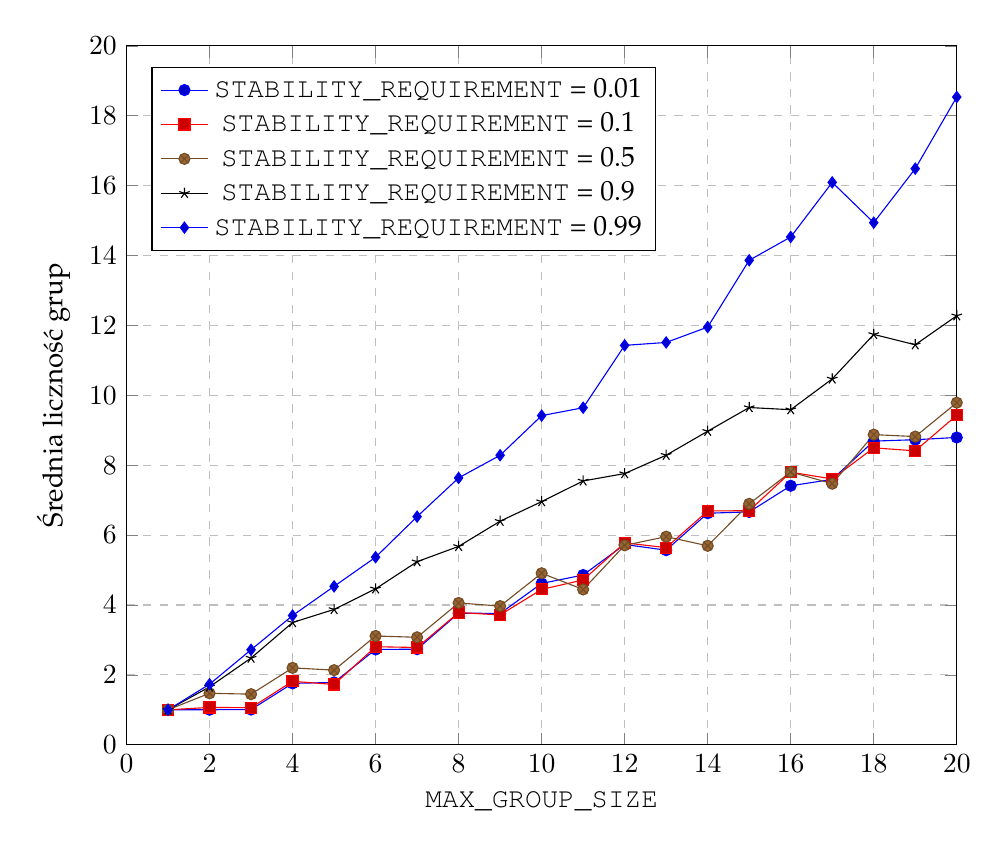
\begin{tikzpicture}
\begin{axis}[
    width=\textwidth,
    xlabel={\texttt{MAX\_GROUP\_SIZE}},
    ylabel={Średnia liczność grup},
    xmin=0, xmax=20,
    ymin=0, ymax=20,
    legend pos=north west,
    ymajorgrids=true,
    xmajorgrids=true,
    grid style=dashed,
]
\addplot coordinates {

(1,1.0)
(2,1.0022988505747126)
(3,1.0074534161490682)
(4,1.7569573283859)
(5,1.7833935018050542)
(6,2.726775956284153)
(7,2.735042735042735)
(8,3.765151515151515)
(9,3.7587548638132295)
(10,4.61611374407583)
(11,4.857142857142857)
(12,5.730337078651686)
(13,5.568181818181818)
(14,6.625850340136054)
(15,6.662337662337662)
(16,7.410852713178294)
(17,7.593984962406015)
(18,8.688524590163935)
(19,8.728813559322035)
(20,8.792792792792794)


};

\addplot coordinates {

(1,1.0)
(2,1.0686922060766182)
(3,1.0605226960110041)
(4,1.8154425612052731)
(5,1.7251461988304093)
(6,2.8049450549450547)
(7,2.7834757834757835)
(8,3.7829457364341086)
(9,3.715302491103203)
(10,4.4454976303317535)
(11,4.715686274509804)
(12,5.777777777777778)
(13,5.640449438202247)
(14,6.6891891891891895)
(15,6.697986577181208)
(16,7.7984496124031)
(17,7.606060606060606)
(18,8.495575221238939)
(19,8.41025641025641)
(20,9.428571428571429)



};

\addplot coordinates {
(1,1.0)
(2,1.4727564102564104)
(3,1.4478632478632478)
(4,2.200440528634361)
(5,2.1343612334801763)
(6,3.112540192926045)
(7,3.074675324675325)
(8,4.057142857142857)
(9,3.968503937007874)
(10,4.907216494845361)
(11,4.443946188340807)
(12,5.705882352941177)
(13,5.955056179775281)
(14,5.6923076923076925)
(15,6.8936170212765955)
(16,7.806451612903226)
(17,7.470149253731344)
(18,8.875)
(19,8.818181818181818)
(20,9.788461538461538)
};

\addplot coordinates {

(1,1.0)
(2,1.6569343065693432)
(3,2.481012658227848)
(4,3.4983050847457626)
(5,3.8725099601593627)
(6,4.461883408071749)
(7,5.238578680203045)
(8,5.676300578034682)
(9,6.397350993377484)
(10,6.957142857142857)
(11,7.548872180451128)
(12,7.76)
(13,8.285714285714286)
(14,8.97196261682243)
(15,9.649484536082474)
(16,9.587628865979381)
(17,10.46808510638298)
(18,11.741176470588234)
(19,11.44578313253012)
(20,12.276315789473685)

};

\addplot coordinates {

(1,1.0)
(2,1.7322097378277153)
(3,2.7183098591549295)
(4,3.696969696969697)
(5,4.5327102803738315)
(6,5.366120218579235)
(7,6.528301886792453)
(8,7.636363636363637)
(9,8.283333333333333)
(10,9.418181818181818)
(11,9.643564356435643)
(12,11.428571428571429)
(13,11.511627906976743)
(14,11.951807228915662)
(15,13.863013698630137)
(16,14.529411764705882)
(17,16.092307692307692)
(18,14.93939393939394)
(19,16.483870967741936)
(20,18.535714285714285)


};

\legend{\texttt{STABILITY\_REQUIREMENT} = 0.01, \texttt{STABILITY\_REQUIREMENT} = 0.1, \texttt{STABILITY\_REQUIREMENT}  = 0.5, \texttt{STABILITY\_REQUIREMENT}  = 0.9, \texttt{STABILITY\_REQUIREMENT}  = 0.99}
\end{axis}
\end{tikzpicture}
\caption{Wykres 6.1: Wpływ parametru \texttt{MAX\_GROUP\_SIZE} wraz z wybranymi wartościami \texttt{STABILITY\_REQUIREMENT} na średnią liczność grup.}
\end{figure}

Wykres 6.2 przedstawia wpływ parametru \texttt{STABILITY\_REQUIREMENT} na średnią liczność grup. Wpływ ten zbadano dla różnych wartości parametru \texttt{RANDOM\_AD}-\texttt{D\_PROBABILITY}. Parametry testu, dla którego powstał wykres 6.2: liczba eksperymentów --- 101, początkowa liczba węzłów --- 1000, liczba cykli --- 1000, maksymalny rozmiar grupy --- 10. Z wykresu wynika, że średnia liczność grup rośnie wraz ze wzrostem parametru \texttt{STABILITY\_REQUIREMENT}. Wzrost średniej liczności grup jest największy dla sytuacji, w której to jest więcej dołączeń niż odłączeń węzłów (parametr \texttt{RANDOM\_ADD\_PROBABILITY} przyjmuje wartości powyżej 0.5); gdy jest jednak więcej odłączeń, niż dołączeń (parametr \texttt{RANDOM\_ADD\_PROBABILITY} przyjmuje wartości poniżej 0.5), wzrost średniej liczności grup jest zdecydowanie mniejszy, a dla skrajnie niskich wartości parametru \texttt{RANDOM\_ADD\_PROBABILITY} (0.01), wzrost średniej liczności jest niezauważalny. Wynika to z faktu, iż gdy w sieci jest więcej odłączeń węzłów, niż dołączeń węzłów, to grupy częściej tracą członków, niż zyskują. Jeżeli jednak więcej węzłów się dołącza niż odłącza, grupy się wypełniają węzłami, co zwiększa ich liczność. Ponadto, przy wysokich wymaganiach odnośnie tworzenia nowych grup (gdy parametr \texttt{STABILITY\_REQUIREMENT} przyjmuje duże wartości), rzadko który węzeł jest na tyle stabilny, aby utworzyć nową grupę, zamiast dołączyć do istniejącej; a więc węzły częściej dołączają do istniejących grup, niż tworzą nowe, co zwiększa średnią liczność grup.

\begin{figure}[H]
\captionsetup{labelformat=empty}
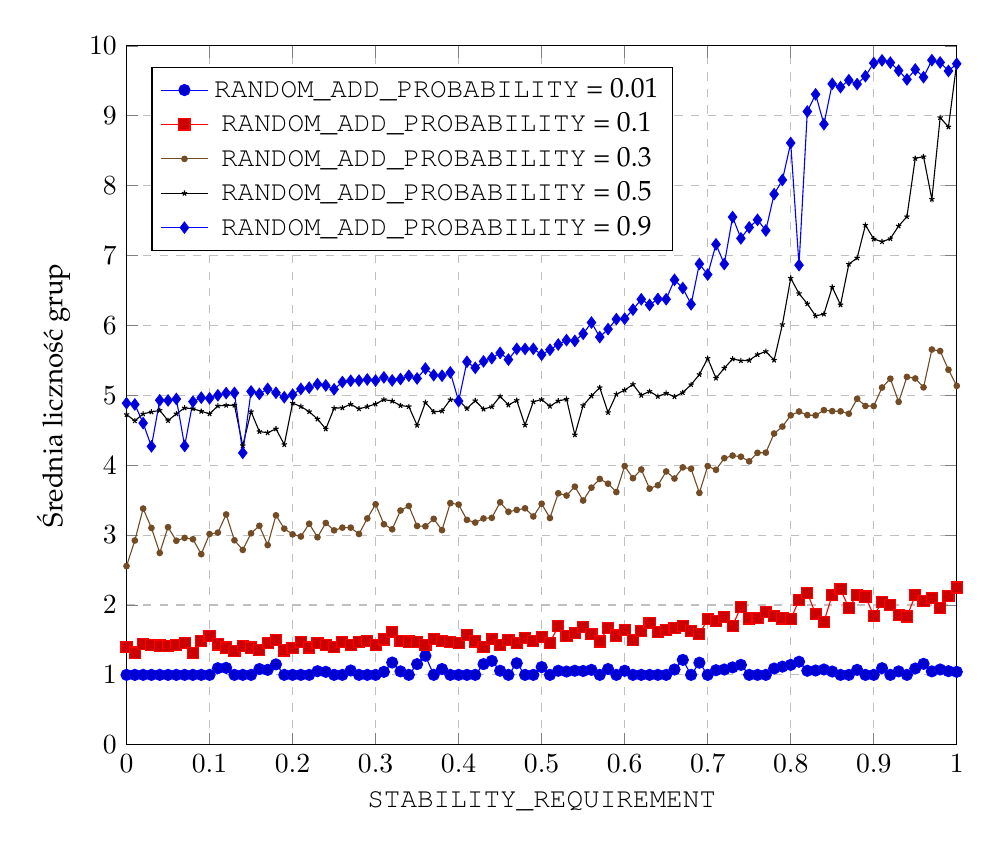
\begin{tikzpicture}
\begin{axis}[
    width=\textwidth,
    xlabel={\texttt{STABILITY\_REQUIREMENT}},
    ylabel={Średnia liczność grup},
    xmin=0, xmax=1,
    ymin=0, ymax=10,
    legend pos=north west,
    ymajorgrids=true,
    xmajorgrids=true,
    grid style=dashed,
]
\addplot coordinates {

(0.0,1.0)
(0.01,1.0)
(0.02,1.0)
(0.03,1.0)
(0.04,1.0)
(0.05,1.0)
(0.06,1.0)
(0.07,1.0)
(0.08,1.0)
(0.09,1.0)
(0.1,1.0)
(0.11,1.0952380952380953)
(0.12,1.1)
(0.13,1.0)
(0.14,1.0)
(0.15,1.0)
(0.16,1.0833333333333333)
(0.17,1.0714285714285714)
(0.18,1.15)
(0.19,1.0)
(0.2,1.0)
(0.21,1.0)
(0.22,1.0)
(0.23,1.0526315789473684)
(0.24,1.0434782608695652)
(0.25,1.0)
(0.26,1.0)
(0.27,1.0625)
(0.28,1.0)
(0.29,1.0)
(0.3,1.0)
(0.31,1.0434782608695652)
(0.32,1.1764705882352942)
(0.33,1.05)
(0.34,1.0)
(0.35000000000000003,1.1538461538461537)
(0.36,1.2727272727272727)
(0.37,1.0)
(0.38,1.0833333333333333)
(0.39,1.0)
(0.4,1.0)
(0.41000000000000003,1.0)
(0.42,1.0)
(0.43,1.1538461538461537)
(0.44,1.2)
(0.45,1.0588235294117647)
(0.46,1.0)
(0.47000000000000003,1.1666666666666667)
(0.48,1.0)
(0.49,1.0)
(0.5,1.1111111111111112)
(0.51,1.0)
(0.52,1.0588235294117647)
(0.53,1.0476190476190477)
(0.54,1.0588235294117647)
(0.55,1.0555555555555556)
(0.56,1.0714285714285714)
(0.5700000000000001,1.0)
(0.58,1.0833333333333333)
(0.59,1.0)
(0.6,1.0588235294117647)
(0.61,1.0)
(0.62,1.0)
(0.63,1.0)
(0.64,1.0)
(0.65,1.0)
(0.66,1.0769230769230769)
(0.67,1.2142857142857142)
(0.68,1.0)
(0.6900000000000001,1.173913043478261)
(0.7000000000000001,1.0)
(0.71,1.0666666666666667)
(0.72,1.0769230769230769)
(0.73,1.1071428571428572)
(0.74,1.1428571428571428)
(0.75,1.0)
(0.76,1.0)
(0.77,1.0)
(0.78,1.0909090909090908)
(0.79,1.1176470588235294)
(0.8,1.1428571428571428)
(0.81,1.1875)
(0.8200000000000001,1.0588235294117647)
(0.8300000000000001,1.0625)
(0.84,1.0769230769230769)
(0.85,1.0476190476190477)
(0.86,1.0)
(0.87,1.0)
(0.88,1.0714285714285714)
(0.89,1.0)
(0.9,1.0)
(0.91,1.0952380952380953)
(0.92,1.0)
(0.93,1.05)
(0.9400000000000001,1.0)
(0.9500000000000001,1.0909090909090908)
(0.96,1.1578947368421053)
(0.97,1.05)
(0.98,1.0769230769230769)
(0.99,1.0526315789473684)
(1.0,1.0434782608695652)


};

\addplot coordinates {

(0.0,1.4)
(0.01,1.319327731092437)
(0.02,1.4444444444444444)
(0.03,1.421487603305785)
(0.04,1.4196428571428572)
(0.05,1.4186046511627908)
(0.06,1.421875)
(0.07,1.4545454545454546)
(0.08,1.3082706766917294)
(0.09,1.4883720930232558)
(0.1,1.5511811023622046)
(0.11,1.434782608695652)
(0.12,1.390625)
(0.13,1.3461538461538463)
(0.14,1.4152542372881356)
(0.15,1.3909774436090225)
(0.16,1.361344537815126)
(0.17,1.4516129032258065)
(0.18,1.5034965034965035)
(0.19,1.3495934959349594)
(0.2,1.385185185185185)
(0.21,1.4666666666666666)
(0.22,1.391304347826087)
(0.23,1.4603174603174602)
(0.24,1.4328358208955223)
(0.25,1.4)
(0.26,1.4758064516129032)
(0.27,1.423728813559322)
(0.28,1.4710144927536233)
(0.29,1.4848484848484849)
(0.3,1.4285714285714286)
(0.31,1.5072463768115942)
(0.32,1.6142857142857143)
(0.33,1.4867256637168142)
(0.34,1.4761904761904763)
(0.35000000000000003,1.472)
(0.36,1.421875)
(0.37,1.5121951219512195)
(0.38,1.4838709677419355)
(0.39,1.4705882352941178)
(0.4,1.4596774193548387)
(0.41000000000000003,1.5725190839694656)
(0.42,1.4778761061946903)
(0.43,1.3928571428571428)
(0.44,1.5081967213114753)
(0.45,1.4285714285714286)
(0.46,1.5044247787610618)
(0.47000000000000003,1.4538461538461538)
(0.48,1.5289256198347108)
(0.49,1.4903846153846154)
(0.5,1.542857142857143)
(0.51,1.456140350877193)
(0.52,1.7)
(0.53,1.5585585585585586)
(0.54,1.596638655462185)
(0.55,1.680672268907563)
(0.56,1.5873015873015872)
(0.5700000000000001,1.4774774774774775)
(0.58,1.6754385964912282)
(0.59,1.5625)
(0.6,1.6470588235294117)
(0.61,1.4952380952380953)
(0.62,1.631578947368421)
(0.63,1.7391304347826086)
(0.64,1.61864406779661)
(0.65,1.6370967741935485)
(0.66,1.6728971962616823)
(0.67,1.694915254237288)
(0.68,1.626086956521739)
(0.6900000000000001,1.5833333333333333)
(0.7000000000000001,1.7966101694915255)
(0.71,1.7727272727272727)
(0.72,1.823008849557522)
(0.73,1.7019230769230769)
(0.74,1.9739130434782608)
(0.75,1.8073394495412844)
(0.76,1.8144329896907216)
(0.77,1.8942307692307692)
(0.78,1.8440366972477065)
(0.79,1.8073394495412844)
(0.8,1.7941176470588236)
(0.81,2.0679611650485437)
(0.8200000000000001,2.1770833333333335)
(0.8300000000000001,1.8686868686868687)
(0.84,1.7578947368421052)
(0.85,2.142857142857143)
(0.86,2.2254901960784315)
(0.87,1.958762886597938)
(0.88,2.1444444444444444)
(0.89,2.12)
(0.9,1.8478260869565217)
(0.91,2.0388349514563107)
(0.92,2.0)
(0.93,1.858695652173913)
(0.9400000000000001,1.8350515463917525)
(0.9500000000000001,2.136842105263158)
(0.96,2.058252427184466)
(0.97,2.097826086956522)
(0.98,1.9545454545454546)
(0.99,2.130434782608696)
(1.0,2.25)




};

\addplot+[mark options={scale=0.5}] coordinates {

(0.0,2.55609756097561)
(0.01,2.9223300970873787)
(0.02,3.3793103448275863)
(0.03,3.102439024390244)
(0.04,2.745)
(0.05,3.1133004926108376)
(0.06,2.918781725888325)
(0.07,2.959798994974874)
(0.08,2.9405940594059405)
(0.09,2.727272727272727)
(0.1,3.0150753768844223)
(0.11,3.0348258706467663)
(0.12,3.295)
(0.13,2.925373134328358)
(0.14,2.787878787878788)
(0.15,3.0251256281407035)
(0.16,3.13265306122449)
(0.17,2.857142857142857)
(0.18,3.282828282828283)
(0.19,3.0918367346938775)
(0.2,3.0103092783505154)
(0.21,2.979591836734694)
(0.22,3.162303664921466)
(0.23,2.9690721649484537)
(0.24,3.1727748691099475)
(0.25,3.0673575129533677)
(0.26,3.106382978723404)
(0.27,3.106382978723404)
(0.28,3.016042780748663)
(0.29,3.238095238095238)
(0.3,3.4408602150537635)
(0.31,3.1550802139037435)
(0.32,3.082901554404145)
(0.33,3.351063829787234)
(0.34,3.4162162162162164)
(0.35000000000000003,3.130434782608696)
(0.36,3.1256830601092895)
(0.37,3.2320441988950277)
(0.38,3.07103825136612)
(0.39,3.4574468085106385)
(0.4,3.43646408839779)
(0.41000000000000003,3.217391304347826)
(0.42,3.17877094972067)
(0.43,3.2375690607734806)
(0.44,3.247191011235955)
(0.45,3.468926553672316)
(0.46,3.3333333333333335)
(0.47000000000000003,3.359550561797753)
(0.48,3.382857142857143)
(0.49,3.2662721893491122)
(0.5,3.4482758620689653)
(0.51,3.244186046511628)
(0.52,3.5976331360946747)
(0.53,3.565714285714286)
(0.54,3.6932515337423313)
(0.55,3.4941176470588236)
(0.56,3.6785714285714284)
(0.5700000000000001,3.8034682080924855)
(0.58,3.7349397590361444)
(0.59,3.6153846153846154)
(0.6,3.9876543209876543)
(0.61,3.813664596273292)
(0.62,3.9382716049382718)
(0.63,3.664516129032258)
(0.64,3.712574850299401)
(0.65,3.91025641025641)
(0.66,3.8089171974522293)
(0.67,3.9683544303797467)
(0.68,3.948717948717949)
(0.6900000000000001,3.603896103896104)
(0.7000000000000001,3.9871794871794872)
(0.71,3.933333333333333)
(0.72,4.1)
(0.73,4.136986301369863)
(0.74,4.120805369127517)
(0.75,4.055172413793104)
(0.76,4.176470588235294)
(0.77,4.17910447761194)
(0.78,4.452554744525547)
(0.79,4.552238805970149)
(0.8,4.713178294573644)
(0.81,4.768)
(0.8200000000000001,4.716666666666667)
(0.8300000000000001,4.712)
(0.84,4.78740157480315)
(0.85,4.7734375)
(0.86,4.770491803278689)
(0.87,4.736)
(0.88,4.95)
(0.89,4.8474576271186445)
(0.9,4.845528455284553)
(0.91,5.111111111111111)
(0.92,5.237288135593221)
(0.93,4.905982905982906)
(0.9400000000000001,5.2631578947368425)
(0.9500000000000001,5.2407407407407405)
(0.96,5.113043478260869)
(0.97,5.654545454545454)
(0.98,5.63302752293578)
(0.99,5.365384615384615)
(1.0,5.134615384615385)

};

\addplot+[mark options={scale=0.5}] coordinates {

(0.0,4.72463768115942)
(0.01,4.6350710900473935)
(0.02,4.733333333333333)
(0.03,4.761904761904762)
(0.04,4.784313725490196)
(0.05,4.6380952380952385)
(0.06,4.734883720930233)
(0.07,4.819047619047619)
(0.08,4.8076923076923075)
(0.09,4.770731707317073)
(0.1,4.734883720930233)
(0.11,4.847926267281106)
(0.12,4.857142857142857)
(0.13,4.8584905660377355)
(0.14,4.28)
(0.15,4.76555023923445)
(0.16,4.480851063829787)
(0.17,4.464285714285714)
(0.18,4.52)
(0.19,4.295154185022026)
(0.2,4.88785046728972)
(0.21,4.839622641509434)
(0.22,4.76555023923445)
(0.23,4.660287081339713)
(0.24,4.518518518518518)
(0.25,4.815533980582524)
(0.26,4.820754716981132)
(0.27,4.872037914691943)
(0.28,4.805825242718447)
(0.29,4.83743842364532)
(0.3,4.875576036866359)
(0.31,4.938967136150235)
(0.32,4.917073170731707)
(0.33,4.852941176470588)
(0.34,4.838383838383838)
(0.35000000000000003,4.570776255707763)
(0.36,4.897560975609756)
(0.37,4.761904761904762)
(0.38,4.775510204081633)
(0.39,4.937799043062201)
(0.4,4.93)
(0.41000000000000003,4.809756097560975)
(0.42,4.923076923076923)
(0.43,4.8019323671497585)
(0.44,4.836538461538462)
(0.45,4.985074626865671)
(0.46,4.861386138613861)
(0.47000000000000003,4.926829268292683)
(0.48,4.57345971563981)
(0.49,4.907766990291262)
(0.5,4.9393939393939394)
(0.51,4.8431372549019605)
(0.52,4.91919191919192)
(0.53,4.944162436548224)
(0.54,4.4343891402714934)
(0.55,4.853658536585366)
(0.56,4.99009900990099)
(0.5700000000000001,5.109947643979058)
(0.58,4.753488372093023)
(0.59,5.014634146341463)
(0.6,5.074626865671642)
(0.61,5.155778894472362)
(0.62,5.0)
(0.63,5.05699481865285)
(0.64,4.983957219251337)
(0.65,5.02970297029703)
(0.66,4.98)
(0.67,5.038251366120218)
(0.68,5.151832460732984)
(0.6900000000000001,5.297297297297297)
(0.7000000000000001,5.528795811518324)
(0.71,5.244897959183674)
(0.72,5.387978142076503)
(0.73,5.52)
(0.74,5.494623655913978)
(0.75,5.5)
(0.76,5.581920903954802)
(0.77,5.627906976744186)
(0.78,5.502890173410405)
(0.79,6.012422360248447)
(0.8,6.675)
(0.81,6.455696202531645)
(0.8200000000000001,6.308641975308642)
(0.8300000000000001,6.135802469135802)
(0.84,6.162162162162162)
(0.85,6.546666666666667)
(0.86,6.294871794871795)
(0.87,6.875816993464053)
(0.88,6.965034965034965)
(0.89,7.43448275862069)
(0.9,7.236111111111111)
(0.91,7.197080291970803)
(0.92,7.240875912408759)
(0.93,7.4222222222222225)
(0.9400000000000001,7.555555555555555)
(0.9500000000000001,8.389830508474576)
(0.96,8.413223140495868)
(0.97,7.804878048780488)
(0.98,8.973451327433628)
(0.99,8.839285714285714)
(1.0,9.757009345794392)


};

\addplot coordinates {

(0.0,4.887096774193548)
(0.01,4.868852459016393)
(0.02,4.601522842639594)
(0.03,4.269047619047619)
(0.04,4.928571428571429)
(0.05,4.926430517711172)
(0.06,4.9476584022038566)
(0.07,4.27511961722488)
(0.08,4.909090909090909)
(0.09,4.966292134831461)
(0.1,4.956043956043956)
(0.11,5.0)
(0.12,5.031161473087819)
(0.13,5.033898305084746)
(0.14,4.176201372997712)
(0.15,5.055865921787709)
(0.16,5.0194986072423395)
(0.17,5.091428571428572)
(0.18,5.03601108033241)
(0.19,4.972222222222222)
(0.2,5.0085227272727275)
(0.21,5.090909090909091)
(0.22,5.109243697478991)
(0.23,5.159090909090909)
(0.24,5.140401146131805)
(0.25,5.085714285714285)
(0.26,5.189504373177843)
(0.27,5.2079772079772075)
(0.28,5.210374639769452)
(0.29,5.226361031518625)
(0.3,5.2105263157894735)
(0.31,5.255813953488372)
(0.32,5.2128279883381925)
(0.33,5.232558139534884)
(0.34,5.279761904761905)
(0.35000000000000003,5.240579710144927)
(0.36,5.382789317507418)
(0.37,5.288629737609329)
(0.38,5.279761904761905)
(0.39,5.327327327327327)
(0.4,4.916897506925208)
(0.41000000000000003,5.4787878787878785)
(0.42,5.392857142857143)
(0.43,5.485029940119761)
(0.44,5.530864197530864)
(0.45,5.60625)
(0.46,5.510703363914373)
(0.47000000000000003,5.663492063492064)
(0.48,5.663551401869159)
(0.49,5.6645962732919255)
(0.5,5.58125)
(0.51,5.651898734177215)
(0.52,5.726114649681529)
(0.53,5.789137380191693)
(0.54,5.778501628664495)
(0.55,5.879598662207358)
(0.56,6.040677966101695)
(0.5700000000000001,5.832797427652733)
(0.58,5.947194719471947)
(0.59,6.088737201365188)
(0.6,6.095238095238095)
(0.61,6.226027397260274)
(0.62,6.373239436619718)
(0.63,6.2926829268292686)
(0.64,6.377224199288256)
(0.65,6.374558303886926)
(0.66,6.651685393258427)
(0.67,6.534798534798535)
(0.68,6.301754385964912)
(0.6900000000000001,6.879699248120301)
(0.7000000000000001,6.726591760299626)
(0.71,7.16)
(0.72,6.877862595419847)
(0.73,7.55)
(0.74,7.244979919678715)
(0.75,7.401639344262295)
(0.76,7.5103734439834025)
(0.77,7.3580246913580245)
(0.78,7.87719298245614)
(0.79,8.08)
(0.8,8.60952380952381)
(0.81,6.862068965517241)
(0.8200000000000001,9.05940594059406)
(0.8300000000000001,9.306122448979592)
(0.84,8.878787878787879)
(0.85,9.455497382198953)
(0.86,9.409326424870466)
(0.87,9.507853403141361)
(0.88,9.452631578947368)
(0.89,9.566137566137566)
(0.9,9.75268817204301)
(0.91,9.791208791208792)
(0.92,9.759562841530055)
(0.93,9.64516129032258)
(0.9400000000000001,9.518716577540108)
(0.9500000000000001,9.66120218579235)
(0.96,9.550802139037433)
(0.97,9.794594594594594)
(0.98,9.762162162162163)
(0.99,9.640211640211641)
(1.0,9.743016759776536)


};

\legend{\texttt{RANDOM\_ADD\_PROBABILITY} = 0.01, \texttt{RANDOM\_ADD\_PROBABILITY} = 0.1, \texttt{RANDOM\_ADD\_PROBABILITY} = 0.3, \texttt{RANDOM\_ADD\_PROBABILITY} = 0.5, \texttt{RANDOM\_ADD\_PROBABILITY} = 0.9}
\end{axis}
\end{tikzpicture}
\caption{Wykres 6.2: Wpływ parametru \texttt{STABILITY\_REQUIREMENT} wraz z wybranymi wartościami \texttt{RANDOM\_ADD\_PROBABILITY} na średnią liczność grup.}
\end{figure}

\subsection{Średni czas życia grup}

Poniżej przedstawiono wyniki testów wpływu parametrów \texttt{MAX\_GROUP\_SIZE} i \texttt{STABILITY\_REQUIREMENT} na średni czas życia grup. Czas życia grupy oznacza liczbę cykli, które minęły od momentu powstania grupy, aż do odłączenia się ostatniego członka grupy.

Wykres 6.3 przedstawia wpływ parametru \texttt{MAX\_GROUP\_SIZE} na średni czas życia grup. Wpływ ten zbadano dla różnych wartości \texttt{STABILITY\_REQUIREMENT}. Parametry testu, dla którego powstał wykres 6.3: liczba eksperymentów --- 20, początkowa liczba węzłów --- 1000, liczba cykli --- 10000, prawdopodobieństwo dołączenia nowego węzła w przypadku zmiany w sieci --- 0.5. Na wykresie 6.3 widać, że dla \texttt{MAX\_GROUP\_SIZE} mniejszego niż 8, średni czas życia grup rośnie wraz ze wzrostem \texttt{MAX\_GROUP\_SIZE}. Ponadto, wzrost ten jest większy dla większych wartości parametrów \texttt{STABILITY\_REQUIREMENT}. Dla \texttt{MAX\_GROUP\_SIZE} większego od 7, średni czas życia grup jest podobny dla różnych wartości parametru \texttt{STABILITY\_REQUIR}-\texttt{EMENT}, i wynosi między 7000 a 10000 -- czyli przez większość cykli pojedynczego eksperymentu. Rozbieżność ta wynika z faktu losowości zachowań w sieci (parametr \texttt{RANDOM} klasy \texttt{RandomDynamicNetwork} równy jest 1) oraz losowości stabilności węzła. Z wykresu 6.3 wynika, że maksymalna liczność grupy, dla której odczuwana jest zmiana wartości parametru  \texttt{STABILITY\_REQUIREMENT} przy symulacji trwającej 10000 cykli --- to 7. Wynika to z faktu, iż im większa grupa, tym mniejsza szansa, że wszyscy członkowie odejdą zanim do grupy dołączy nowy węzeł (co skutkuje zakończeniem życia grupy). Maksymalna liczność grupy równa 8, jest wystarczająca, aby grupy żyły średnio przez większość z 10000 cykli.

\begin{figure}[H]
\captionsetup{labelformat=empty}
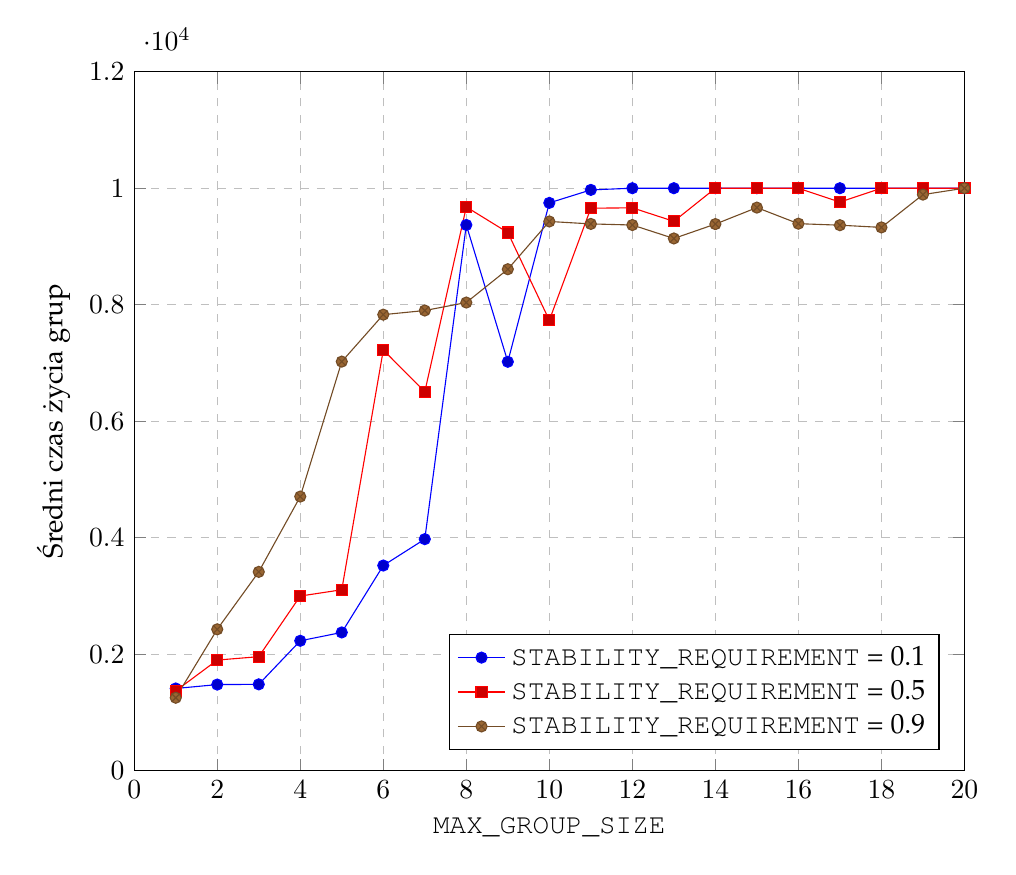
\begin{tikzpicture}
\begin{axis}[
    width=\textwidth,
    xlabel={\texttt{MAX\_GROUP\_SIZE}},
    ylabel={Średni czas życia grup},
    xmin=0, xmax=20,
    ymin=0, ymax=12000,
    legend pos=south east,
    ymajorgrids=true,
    xmajorgrids=true,
    grid style=dashed,
]

\addplot coordinates {

(1,1411)
(2,1478)
(3,1482)
(4,2230)
(5,2373)
(6,3522)
(7,3975)
(8,9369)
(9,7020)
(10,9748)
(11,9971)
(12,10000)
(13,10000)
(14,10000)
(15,10000)
(16,10000)
(17,10000)
(18,10000)
(19,10000)
(20,10000)

};

\addplot coordinates {

(1,1369)
(2,1899)
(3,1957)
(4,2998)
(5,3106)
(6,7222)
(7,6505)
(8,9678)
(9,9239)
(10,7732)
(11,9657)
(12,9663)
(13,9431)
(14,10000)
(15,10000)
(16,10000)
(17,9761)
(18,10000)
(19,10000)
(20,10000)

};

\addplot coordinates {

(1,1252)
(2,2427)
(3,3413)
(4,4706)
(5,7023)
(6,7829)
(7,7900)
(8,8037)
(9,8609)
(10,9429)
(11,9387)
(12,9368)
(13,9137)
(14,9384)
(15,9667)
(16,9391)
(17,9365)
(18,9327)
(19,9890)
(20,10000)

};

\legend{\texttt{STABILITY\_REQUIREMENT} = 0.1, \texttt{STABILITY\_REQUIREMENT} = 0.5, \texttt{STABILITY\_REQUIREMENT} = 0.9}
\end{axis}
\end{tikzpicture}
\caption{Wykres 6.3: Wpływ parametru \texttt{MAX\_GROUP\_SIZE} wraz z wybranymi wartościami \texttt{STABILITY\_REQUIREMENT} na średni czas życia grup.}
\end{figure}

Wykres 6.4 przedstawia wpływ parametru \texttt{STABILITY\_REQUIREMENT} na średni czas życia grup. Wpływ ten zbadano dla różnych wartości \texttt{MAX\_GROUP\_SIZE}. Parametry testu, dla którego powstał wykres 6.4: liczba eksperymentów --- 21, początkowa liczba węzłów --- 1000, liczba cykli --- 10000, prawdopodobieństwo dołączenia nowego węzła w przypadku zmiany w sieci --- 0.5. Na wykresie 6.4 widać, że dla maksymalnej liczności grup równej 3, 5 lub 7, wraz z wzrostem parametru \texttt{STABILITY\_REQUIREMENT} wzrasta średni czas życia grup --- przy czym wzrost ten jest największy dla wysokich wartości \texttt{STABILITY\_REQUIREMENT} (od 0.6 do 1). Zależność ta nie jest widoczna dla przypadku, w którym parametr \texttt{MAX\_GROUP\_SIZE} równy jest 10, lub 20 -- wtenczas średni czas życia grup waha się od 6000 do 10000 dla dowolnej wartości \texttt{STABILITY\_REQUIREMENT}, a dla \texttt{STABILITY\_REQUIREMENT} wyższego od 0.4, średni czas życia grup waha się od 8854 od 10000. Wahania te wynikają z losowości zachowań węzłów w sieci oraz losowości w wyznaczaniu stabilności. Zmiana parametru \texttt{STABILITY\_REQUIREMENT} nie wpływa znacząco na średni czas życia grup dla \texttt{MAX\_GROUP\_SIZE} równego 10, lub 20, ponieważ w tych wypadkach grupy są na tyle liczne, że mała jest szansa, aby w przeciągu 10000 cykli zginęły z powodu odejścia wszystkich członków.

\begin{figure}[H]
\captionsetup{labelformat=empty}
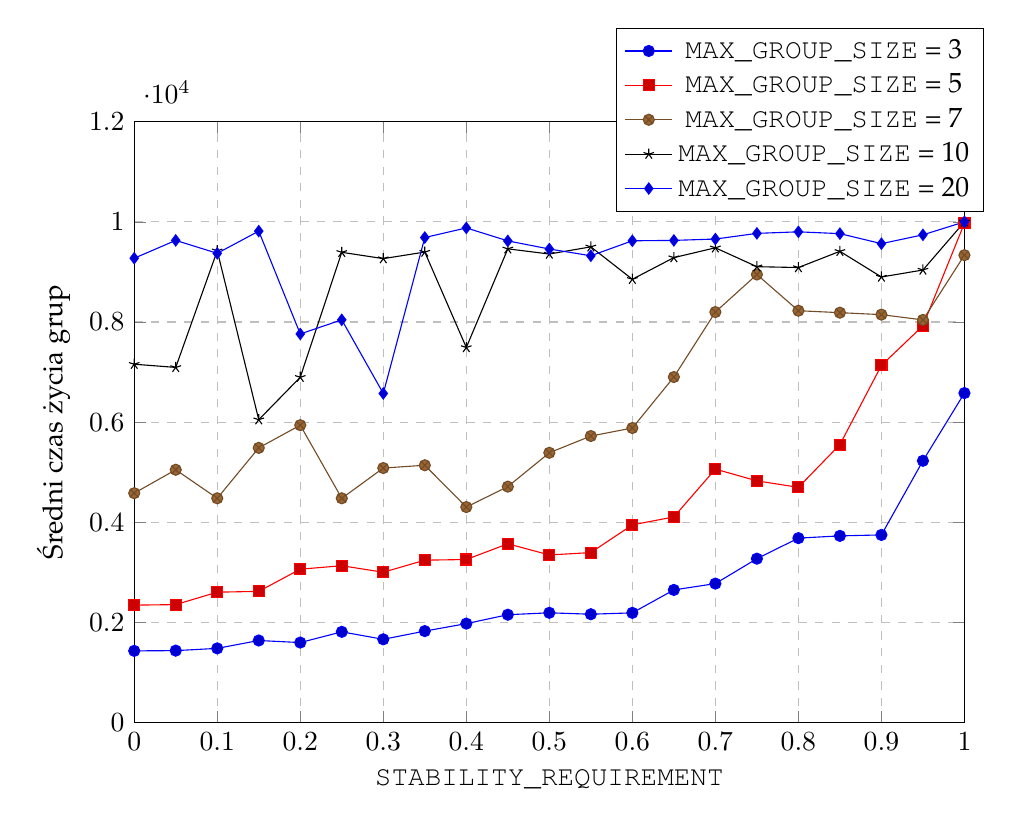
\begin{tikzpicture}
\begin{axis}[
    width=\textwidth,
    height=0.76\textwidth,
    xlabel={\texttt{STABILITY\_REQUIREMENT}},
    ylabel={Średni czas życia grup},
    xmin=0, xmax=1,
    ymin=0, ymax=12000,
    %legend pos=south east,
    legend style={
		at={(0.58,0.85)},
		anchor=south west},
    ymajorgrids=true,
    xmajorgrids=true,
    grid style=dashed,
]
\addplot coordinates {

(0.0,1435)
(0.05,1440)
(0.1,1485)
(0.15000000000000002,1642)
(0.2,1601)
(0.25,1815)
(0.30000000000000004,1666)
(0.35000000000000003,1830)
(0.4,1979)
(0.45,2157)
(0.5,2195)
(0.55,2167)
(0.6000000000000001,2194)
(0.65,2652)
(0.7000000000000001,2778)
(0.75,3276)
(0.8,3686)
(0.8500000000000001,3731)
(0.9,3750)
(0.9500000000000001,5230)
(1.0,6582)

};

\addplot coordinates {

(0.0,2348)
(0.05,2359)
(0.1,2607)
(0.15000000000000002,2623)
(0.2,3066)
(0.25,3135)
(0.30000000000000004,3005)
(0.35000000000000003,3246)
(0.4,3259)
(0.45,3573)
(0.5,3350)
(0.55,3397)
(0.6000000000000001,3951)
(0.65,4109)
(0.7000000000000001,5064)
(0.75,4829)
(0.8,4700)
(0.8500000000000001,5553)
(0.9,7135)
(0.9500000000000001,7925)
(1.0,9974)


};

\addplot coordinates {

(0.0,4583)
(0.05,5051)
(0.1,4481)
(0.15000000000000002,5488)
(0.2,5941)
(0.25,4481)
(0.30000000000000004,5085)
(0.35000000000000003,5141)
(0.4,4306)
(0.45,4714)
(0.5,5390)
(0.55,5724)
(0.6000000000000001,5884)
(0.65,6902)
(0.7000000000000001,8199)
(0.75,8949)
(0.8,8226)
(0.8500000000000001,8187)
(0.9,8148)
(0.9500000000000001,8042)
(1.0,9335)


};

\addplot coordinates {

(0.0,7158)
(0.05,7094)
(0.1,9423)
(0.15000000000000002,6050)
(0.2,6898)
(0.25,9392)
(0.30000000000000004,9266)
(0.35000000000000003,9397)
(0.4,7492)
(0.45,9461)
(0.5,9358)
(0.55,9501)
(0.6000000000000001,8854)
(0.65,9286)
(0.7000000000000001,9482)
(0.75,9105)
(0.8,9088)
(0.8500000000000001,9412)
(0.9,8899)
(0.9500000000000001,9039)
(1.0,10000)

};

\addplot coordinates {

(0.0,9274)
(0.05,9630)
(0.1,9372)
(0.15000000000000002,9815)
(0.2,7762)
(0.25,8044)
(0.30000000000000004,6574)
(0.35000000000000003,9687)
(0.4,9879)
(0.45,9620)
(0.5,9458)
(0.55,9323)
(0.6000000000000001,9622)
(0.65,9630)
(0.7000000000000001,9657)
(0.75,9770)
(0.8,9801)
(0.8500000000000001,9765)
(0.9,9565)
(0.9500000000000001,9741)
(1.0,10000)

};

\legend{\texttt{MAX\_GROUP\_SIZE} = 3, \texttt{MAX\_GROUP\_SIZE} = 5, \texttt{MAX\_GROUP\_SIZE} = 7, \texttt{MAX\_GROUP\_SIZE} = 10, \texttt{MAX\_GROUP\_SIZE} = 20}
\end{axis}
\end{tikzpicture}
\caption{Wykres 6.4: Wpływ parametru \texttt{STABILITY\_REQUIREMENT} wraz z wybranymi wartościami \texttt{MAX\_GROUP\_SIZE} na średni czas życia grup.}
\end{figure}




\begin{comment}



\begin{figure}[H]
\captionsetup{labelformat=empty}
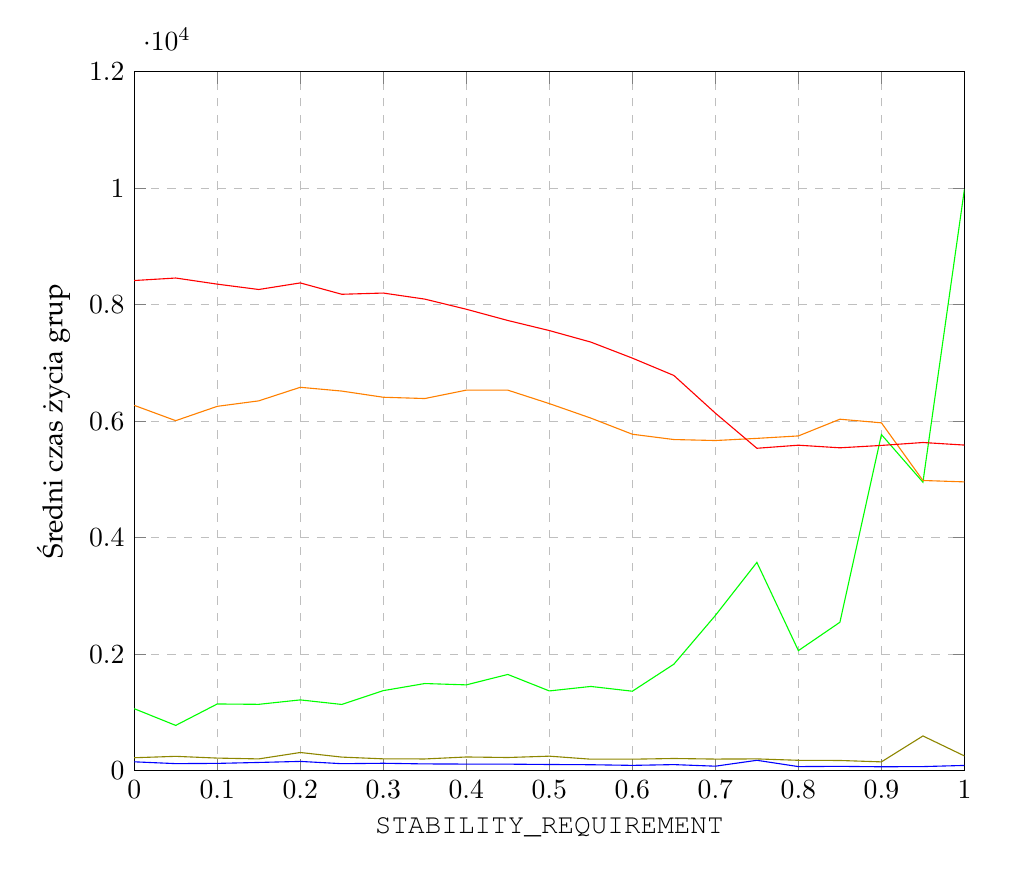
\begin{tikzpicture}
\begin{axis}[
    width=\textwidth,
    xlabel={\texttt{STABILITY\_REQUIREMENT}},
    ylabel={Średni czas życia grup},
    xmin=0, xmax=1,
    ymin=0, ymax=12000,
    %legend pos=south east,
    legend style={
		at={(0.58,0.85)},
		anchor=south west},
    ymajorgrids=true,
    xmajorgrids=true,
    grid style=dashed,
]

\addplot[ color=blue ] coordinates {

(0.0,152)
(0.05,121)
(0.1,125)
(0.15000000000000002,141)
(0.2,159)
(0.25,120)
(0.30000000000000004,127)
(0.35000000000000003,116)
(0.4,113)
(0.45,112)
(0.5,106)
(0.55,102)
(0.6000000000000001,91)
(0.65,104)
(0.7000000000000001,77)
(0.75,178)
(0.8,70)
(0.8500000000000001,74)
(0.9,67)
(0.9500000000000001,70)
(1.0,90)

};

\addplot[ color=olive ] coordinates {

(0.0,222)
(0.05,246)
(0.1,216)
(0.15000000000000002,202)
(0.2,312)
(0.25,233)
(0.30000000000000004,203)
(0.35000000000000003,201)
(0.4,235)
(0.45,226)
(0.5,249)
(0.55,197)
(0.6000000000000001,197)
(0.65,209)
(0.7000000000000001,199)
(0.75,202)
(0.8,178)
(0.8500000000000001,175)
(0.9,151)
(0.9500000000000001,596)
(1.0,253)

};

\addplot[ color=green ] coordinates {

(0.0,1064)
(0.05,777)
(0.1,1145)
(0.15000000000000002,1139)
(0.2,1215)
(0.25,1137)
(0.30000000000000004,1374)
(0.35000000000000003,1496)
(0.4,1473)
(0.45,1652)
(0.5,1369)
(0.55,1446)
(0.6000000000000001,1364)
(0.65,1828)
(0.7000000000000001,2665)
(0.75,3576)
(0.8,2061)
(0.8500000000000001,2548)
(0.9,5770)
(0.9500000000000001,4953)
(1.0,9984)


};

\addplot[ color=orange ] coordinates {

(0.0,6272)
(0.05,6009)
(0.1,6255)
(0.15000000000000002,6349)
(0.2,6582)
(0.25,6517)
(0.30000000000000004,6411)
(0.35000000000000003,6389)
(0.4,6533)
(0.45,6533)
(0.5,6302)
(0.55,6053)
(0.6000000000000001,5776)
(0.65,5685)
(0.7000000000000001,5668)
(0.75,5705)
(0.8,5747)
(0.8500000000000001,6034)
(0.9,5972)
(0.9500000000000001,4982)
(1.0,4958)


};

\addplot[ color=red ] coordinates {

(0.0,8415)
(0.05,8458)
(0.1,8353)
(0.15000000000000002,8261)
(0.2,8374)
(0.25,8179)
(0.30000000000000004,8200)
(0.35000000000000003,8096)
(0.4,7922)
(0.45,7729)
(0.5,7556)
(0.55,7358)
(0.6000000000000001,7083)
(0.65,6785)
(0.7000000000000001,6138)
(0.75,5535)
(0.8,5588)
(0.8500000000000001,5543)
(0.9,5584)
(0.9500000000000001,5634)
(1.0,5590)


};


\end{axis}
\end{tikzpicture}
\caption{}
\end{figure}




\begin{figure}[H]
\captionsetup{labelformat=empty}
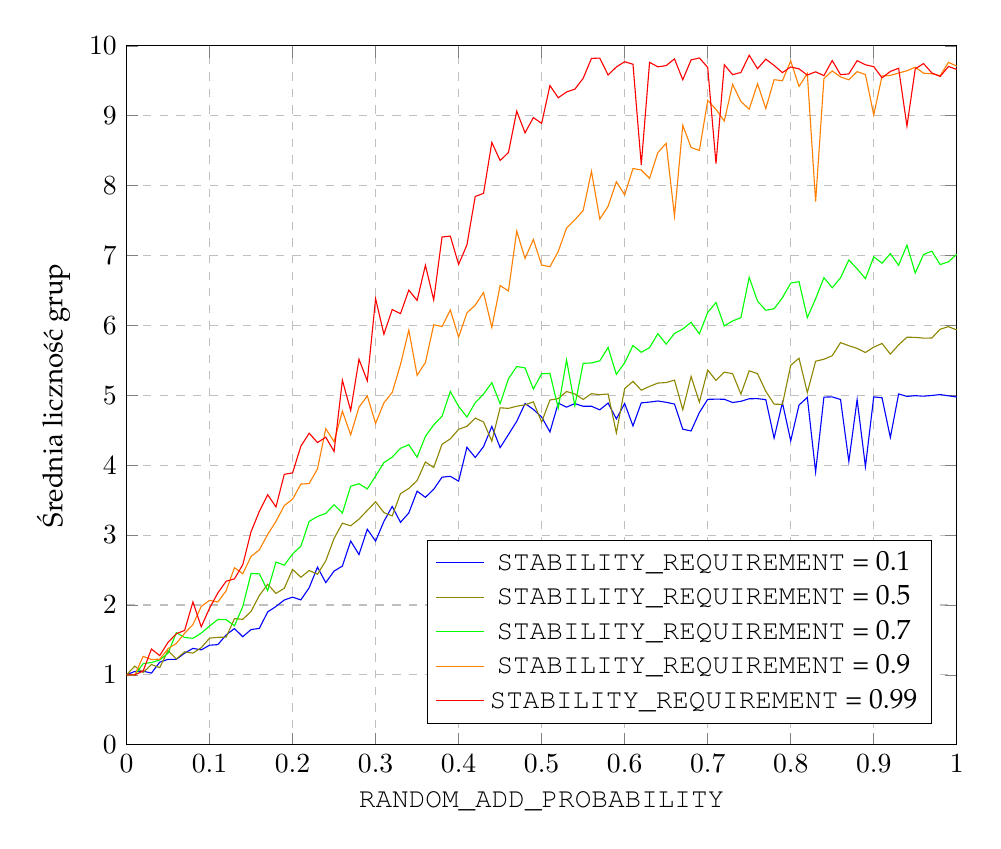
\begin{tikzpicture}
\begin{axis}[
    width=\textwidth,
    xlabel={\texttt{RANDOM\_ADD\_PROBABILITY}},
    ylabel={Średnia liczność grup},
    xmin=0, xmax=1,
    ymin=0, ymax=10,
    legend pos=south east,
    ymajorgrids=true,
    xmajorgrids=true,
    grid style=dashed,
]
\addplot[ color=blue ] coordinates {

	(0.0,1.0)
	(0.01,1.05)
	(0.02,1.0526315789473684)
	(0.03,1.0256410256410255)
	(0.04,1.1818181818181819)
	(0.05,1.2222222222222223)
	(0.06,1.2222222222222223)
	(0.07,1.31)
	(0.08,1.3793103448275863)
	(0.09,1.3571428571428572)
	(0.1,1.4242424242424243)
	(0.11,1.4326241134751774)
	(0.12,1.5714285714285714)
	(0.13,1.6627218934911243)
	(0.14,1.5454545454545454)
	(0.15,1.6484848484848484)
	(0.16,1.6646341463414633)
	(0.17,1.9)
	(0.18,1.9788359788359788)
	(0.19,2.07103825136612)
	(0.2,2.1122994652406417)
	(0.21,2.0726256983240225)
	(0.22,2.2474747474747474)
	(0.23,2.5408163265306123)
	(0.24,2.32)
	(0.25,2.484848484848485)
	(0.26,2.557213930348259)
	(0.27,2.9145728643216082)
	(0.28,2.7213930348258706)
	(0.29,3.083743842364532)
	(0.3,2.914141414141414)
	(0.31,3.1959798994974875)
	(0.32,3.41)
	(0.33,3.1822660098522166)
	(0.34,3.3168316831683167)
	(0.35000000000000003,3.628140703517588)
	(0.36,3.54040404040404)
	(0.37,3.6551724137931036)
	(0.38,3.8282828282828283)
	(0.39,3.8407960199004973)
	(0.4,3.771144278606965)
	(0.41000000000000003,4.25615763546798)
	(0.42,4.11)
	(0.43,4.264705882352941)
	(0.44,4.554455445544554)
	(0.45,4.251256281407035)
	(0.46,4.437810945273632)
	(0.47000000000000003,4.627450980392157)
	(0.48,4.882629107981221)
	(0.49,4.7981220657277)
	(0.5,4.688995215311005)
	(0.51,4.475555555555555)
	(0.52,4.88785046728972)
	(0.53,4.830188679245283)
	(0.54,4.881057268722467)
	(0.55,4.842592592592593)
	(0.56,4.84304932735426)
	(0.5700000000000001,4.791666666666667)
	(0.58,4.8884297520661155)
	(0.59,4.662745098039216)
	(0.6,4.882591093117409)
	(0.61,4.562043795620438)
	(0.62,4.891666666666667)
	(0.63,4.902723735408561)
	(0.64,4.918287937743191)
	(0.65,4.899628252788104)
	(0.66,4.875)
	(0.67,4.514851485148514)
	(0.68,4.489864864864865)
	(0.6900000000000001,4.7534246575342465)
	(0.7000000000000001,4.942028985507246)
	(0.71,4.944827586206896)
	(0.72,4.943262411347518)
	(0.73,4.8966666666666665)
	(0.74,4.913907284768212)
	(0.75,4.95016611295681)
	(0.76,4.9520547945205475)
	(0.77,4.937704918032787)
	(0.78,4.388101983002833)
	(0.79,4.895061728395062)
	(0.8,4.349162011173185)
	(0.81,4.859756097560975)
	(0.8200000000000001,4.969879518072289)
	(0.8300000000000001,3.9039812646370025)
	(0.84,4.973607038123167)
	(0.85,4.976878612716763)
	(0.86,4.939828080229226)
	(0.87,4.053864168618267)
	(0.88,4.938888888888889)
	(0.89,3.9793103448275864)
	(0.9,4.977653631284916)
	(0.91,4.96398891966759)
	(0.92,4.396634615384615)
	(0.93,5.018970189701897)
	(0.9400000000000001,4.983870967741935)
	(0.9500000000000001,4.994791666666667)
	(0.96,4.986945169712794)
	(0.97,4.997416020671834)
	(0.98,5.01025641025641)
	(0.99,4.992443324937028)
	(1.0,4.975124378109452)


};

\addplot[ color=olive ] coordinates {

	(0.0,1.0)
	(0.01,1.125)
	(0.02,1.0333333333333334)
	(0.03,1.1481481481481481)
	(0.04,1.103448275862069)
	(0.05,1.3478260869565217)
	(0.06,1.2277227722772277)
	(0.07,1.3298969072164948)
	(0.08,1.3113207547169812)
	(0.09,1.3888888888888888)
	(0.1,1.525)
	(0.11,1.537190082644628)
	(0.12,1.5396825396825398)
	(0.13,1.8051948051948052)
	(0.14,1.7943262411347518)
	(0.15,1.908496732026144)
	(0.16,2.1363636363636362)
	(0.17,2.2962962962962963)
	(0.18,2.1656050955414012)
	(0.19,2.238993710691824)
	(0.2,2.5090909090909093)
	(0.21,2.396449704142012)
	(0.22,2.4939759036144578)
	(0.23,2.439306358381503)
	(0.24,2.632768361581921)
	(0.25,2.9520958083832336)
	(0.26,3.1705882352941175)
	(0.27,3.132183908045977)
	(0.28,3.2280701754385963)
	(0.29,3.3529411764705883)
	(0.3,3.476470588235294)
	(0.31,3.32183908045977)
	(0.32,3.2742857142857145)
	(0.33,3.593220338983051)
	(0.34,3.6666666666666665)
	(0.35000000000000003,3.7803468208092488)
	(0.36,4.045977011494253)
	(0.37,3.966666666666667)
	(0.38,4.298342541436464)
	(0.39,4.376344086021505)
	(0.4,4.5136612021857925)
	(0.41000000000000003,4.555555555555555)
	(0.42,4.6740331491712706)
	(0.43,4.6187845303867405)
	(0.44,4.343915343915344)
	(0.45,4.821052631578947)
	(0.46,4.8125)
	(0.47000000000000003,4.84375)
	(0.48,4.862944162436548)
	(0.49,4.906403940886699)
	(0.5,4.617511520737327)
	(0.51,4.9326923076923075)
	(0.52,4.9523809523809526)
	(0.53,5.053921568627451)
	(0.54,5.018867924528302)
	(0.55,4.940639269406392)
	(0.56,5.023041474654378)
	(0.5700000000000001,5.008771929824562)
	(0.58,5.018348623853211)
	(0.59,4.462745098039216)
	(0.6,5.096234309623431)
	(0.61,5.198347107438017)
	(0.62,5.073170731707317)
	(0.63,5.127572016460905)
	(0.64,5.174603174603175)
	(0.65,5.182539682539683)
	(0.66,5.217054263565892)
	(0.67,4.794223826714801)
	(0.68,5.269230769230769)
	(0.6900000000000001,4.9020979020979025)
	(0.7000000000000001,5.360594795539034)
	(0.71,5.213483146067416)
	(0.72,5.330798479087452)
	(0.73,5.309608540925267)
	(0.74,5.017123287671233)
	(0.75,5.35)
	(0.76,5.309859154929577)
	(0.77,5.057046979865772)
	(0.78,4.873015873015873)
	(0.79,4.869565217391305)
	(0.8,5.428571428571429)
	(0.81,5.530612244897959)
	(0.8200000000000001,5.039156626506024)
	(0.8300000000000001,5.486666666666666)
	(0.84,5.516129032258065)
	(0.85,5.565789473684211)
	(0.86,5.7540453074433655)
	(0.87,5.709150326797386)
	(0.88,5.670967741935484)
	(0.89,5.6125)
	(0.9,5.688888888888889)
	(0.91,5.7413249211356465)
	(0.92,5.588957055214724)
	(0.93,5.7213622291021675)
	(0.9400000000000001,5.830721003134796)
	(0.9500000000000001,5.82874617737003)
	(0.96,5.817629179331307)
	(0.97,5.819277108433735)
	(0.98,5.945121951219512)
	(0.99,5.9818181818181815)
	(1.0,5.9347181008902075)


};

\addplot[ color=green ] coordinates {

(0.0,1.0)
(0.01,1.0)
(0.02,1.16)
(0.03,1.1764705882352942)
(0.04,1.2127659574468086)
(0.05,1.3103448275862069)
(0.06,1.6046511627906976)
(0.07,1.5348837209302326)
(0.08,1.5238095238095237)
(0.09,1.5977011494252873)
(0.1,1.6979166666666667)
(0.11,1.792)
(0.12,1.7903225806451613)
(0.13,1.7016129032258065)
(0.14,1.9765625)
(0.15,2.450381679389313)
(0.16,2.4453125)
(0.17,2.204379562043796)
(0.18,2.6142857142857143)
(0.19,2.5693430656934306)
(0.2,2.72972972972973)
(0.21,2.8410596026490067)
(0.22,3.195945945945946)
(0.23,3.265734265734266)
(0.24,3.310344827586207)
(0.25,3.43448275862069)
(0.26,3.315068493150685)
(0.27,3.6986301369863015)
(0.28,3.7350993377483444)
(0.29,3.6598639455782314)
(0.3,3.8451612903225807)
(0.31,4.0375)
(0.32,4.115384615384615)
(0.33,4.241610738255034)
(0.34,4.292993630573249)
(0.35000000000000003,4.113924050632911)
(0.36,4.4125)
(0.37,4.576923076923077)
(0.38,4.7006369426751595)
(0.39,5.053892215568863)
(0.4,4.841463414634147)
(0.41000000000000003,4.688622754491018)
(0.42,4.893491124260355)
(0.43,5.017543859649122)
(0.44,5.181286549707602)
(0.45,4.879310344827586)
(0.46,5.236363636363636)
(0.47000000000000003,5.411111111111111)
(0.48,5.392265193370166)
(0.49,5.090425531914893)
(0.5,5.308108108108108)
(0.51,5.3121693121693125)
(0.52,4.8173076923076925)
(0.53,5.505050505050505)
(0.54,4.850467289719626)
(0.55,5.457286432160804)
(0.56,5.462686567164179)
(0.5700000000000001,5.49238578680203)
(0.58,5.684210526315789)
(0.59,5.299539170506913)
(0.6,5.465437788018433)
(0.61,5.712918660287081)
(0.62,5.614349775784754)
(0.63,5.681818181818182)
(0.64,5.881818181818182)
(0.65,5.7309417040358746)
(0.66,5.88479262672811)
(0.67,5.947826086956522)
(0.68,6.044642857142857)
(0.6900000000000001,5.878787878787879)
(0.7000000000000001,6.185022026431718)
(0.71,6.327433628318584)
(0.72,5.991735537190083)
(0.73,6.063291139240507)
(0.74,6.110169491525424)
(0.75,6.686695278969957)
(0.76,6.346774193548387)
(0.77,6.216867469879518)
(0.78,6.238095238095238)
(0.79,6.395161290322581)
(0.8,6.604838709677419)
(0.81,6.625514403292181)
(0.8200000000000001,6.111111111111111)
(0.8300000000000001,6.381322957198444)
(0.84,6.682730923694779)
(0.85,6.538461538461538)
(0.86,6.679841897233201)
(0.87,6.936507936507937)
(0.88,6.809338521400778)
(0.89,6.669201520912548)
(0.9,6.980842911877395)
(0.91,6.889733840304182)
(0.92,7.026819923371647)
(0.93,6.860294117647059)
(0.9400000000000001,7.14828897338403)
(0.9500000000000001,6.75)
(0.96,7.014598540145985)
(0.97,7.061371841155235)
(0.98,6.870175438596491)
(0.99,6.909722222222222)
(1.0,7.017543859649122)


};

\addplot[ color=orange ] coordinates {

	(0.0,1.0)
	(0.01,1.0)
	(0.02,1.2647058823529411)
	(0.03,1.2195121951219512)
	(0.04,1.2244897959183674)
	(0.05,1.375)
	(0.06,1.45)
	(0.07,1.5952380952380953)
	(0.08,1.7195121951219512)
	(0.09,1.9791666666666667)
	(0.1,2.065934065934066)
	(0.11,2.043010752688172)
	(0.12,2.203883495145631)
	(0.13,2.533333333333333)
	(0.14,2.4466019417475726)
	(0.15,2.6936936936936937)
	(0.16,2.7884615384615383)
	(0.17,3.0093457943925235)
	(0.18,3.196261682242991)
	(0.19,3.4220183486238533)
	(0.2,3.5135135135135136)
	(0.21,3.72972972972973)
	(0.22,3.736842105263158)
	(0.23,3.9473684210526314)
	(0.24,4.522123893805309)
	(0.25,4.336134453781512)
	(0.26,4.773109243697479)
	(0.27,4.434782608695652)
	(0.28,4.830508474576271)
	(0.29,4.991596638655462)
	(0.3,4.598360655737705)
	(0.31,4.890756302521009)
	(0.32,5.040650406504065)
	(0.33,5.44)
	(0.34,5.932773109243698)
	(0.35000000000000003,5.285714285714286)
	(0.36,5.46875)
	(0.37,6.0078740157480315)
	(0.38,5.984962406015038)
	(0.39,6.21969696969697)
	(0.4,5.833333333333333)
	(0.41000000000000003,6.17910447761194)
	(0.42,6.2898550724637685)
	(0.43,6.470588235294118)
	(0.44,5.969924812030075)
	(0.45,6.569343065693431)
	(0.46,6.492957746478873)
	(0.47000000000000003,7.348484848484849)
	(0.48,6.957746478873239)
	(0.49,7.229629629629629)
	(0.5,6.86231884057971)
	(0.51,6.839160839160839)
	(0.52,7.057971014492754)
	(0.53,7.391304347826087)
	(0.54,7.510204081632653)
	(0.55,7.642857142857143)
	(0.56,8.204081632653061)
	(0.5700000000000001,7.52054794520548)
	(0.58,7.702702702702703)
	(0.59,8.054421768707483)
	(0.6,7.868421052631579)
	(0.61,8.244897959183673)
	(0.62,8.222972972972974)
	(0.63,8.103896103896103)
	(0.64,8.473684210526315)
	(0.65,8.604026845637584)
	(0.66,7.565714285714286)
	(0.67,8.862745098039216)
	(0.68,8.545454545454545)
	(0.6900000000000001,8.50314465408805)
	(0.7000000000000001,9.217948717948717)
	(0.71,9.090909090909092)
	(0.72,8.924050632911392)
	(0.73,9.448717948717949)
	(0.74,9.20253164556962)
	(0.75,9.093167701863354)
	(0.76,9.45679012345679)
	(0.77,9.103030303030303)
	(0.78,9.515151515151516)
	(0.79,9.5)
	(0.8,9.784431137724551)
	(0.81,9.418604651162791)
	(0.8200000000000001,9.602339181286549)
	(0.8300000000000001,7.771028037383178)
	(0.84,9.531428571428572)
	(0.85,9.640449438202246)
	(0.86,9.554347826086957)
	(0.87,9.513513513513514)
	(0.88,9.630434782608695)
	(0.89,9.58918918918919)
	(0.9,9.010204081632653)
	(0.91,9.56842105263158)
	(0.92,9.576719576719576)
	(0.93,9.61025641025641)
	(0.9400000000000001,9.642857142857142)
	(0.9500000000000001,9.693877551020408)
	(0.96,9.608040201005025)
	(0.97,9.6)
	(0.98,9.572815533980583)
	(0.99,9.763546798029557)
	(1.0,9.70873786407767)


};

\addplot[ color=red ] coordinates {

	(0.0,1.0)
	(0.01,1.0)
	(0.02,1.0555555555555556)
	(0.03,1.3695652173913044)
	(0.04,1.2758620689655173)
	(0.05,1.4655172413793103)
	(0.06,1.588235294117647)
	(0.07,1.6363636363636365)
	(0.08,2.0444444444444443)
	(0.09,1.6883116883116882)
	(0.1,1.9545454545454546)
	(0.11,2.172043010752688)
	(0.12,2.3398058252427183)
	(0.13,2.3737373737373737)
	(0.14,2.5757575757575757)
	(0.15,3.0485436893203883)
	(0.16,3.3398058252427183)
	(0.17,3.576923076923077)
	(0.18,3.4038461538461537)
	(0.19,3.869158878504673)
	(0.2,3.889908256880734)
	(0.21,4.271844660194175)
	(0.22,4.457142857142857)
	(0.23,4.3238095238095235)
	(0.24,4.4)
	(0.25,4.196261682242991)
	(0.26,5.214953271028038)
	(0.27,4.780952380952381)
	(0.28,5.514563106796117)
	(0.29,5.205607476635514)
	(0.3,6.380952380952381)
	(0.31,5.875)
	(0.32,6.226415094339623)
	(0.33,6.168224299065421)
	(0.34,6.5046728971962615)
	(0.35000000000000003,6.357142857142857)
	(0.36,6.859813084112149)
	(0.37,6.363636363636363)
	(0.38,7.264150943396227)
	(0.39,7.277777777777778)
	(0.4,6.872727272727273)
	(0.41000000000000003,7.150442477876106)
	(0.42,7.844660194174757)
	(0.43,7.888888888888889)
	(0.44,8.616822429906541)
	(0.45,8.358490566037736)
	(0.46,8.472727272727273)
	(0.47000000000000003,9.065420560747663)
	(0.48,8.754716981132075)
	(0.49,8.972477064220184)
	(0.5,8.89090909090909)
	(0.51,9.431192660550458)
	(0.52,9.256637168141593)
	(0.53,9.339449541284404)
	(0.54,9.379310344827585)
	(0.55,9.53448275862069)
	(0.56,9.81981981981982)
	(0.5700000000000001,9.824561403508772)
	(0.58,9.583333333333334)
	(0.59,9.697478991596638)
	(0.6,9.772357723577235)
	(0.61,9.736434108527131)
	(0.62,8.297297297297296)
	(0.63,9.763779527559056)
	(0.64,9.699248120300751)
	(0.65,9.716417910447761)
	(0.66,9.8125)
	(0.67,9.514285714285714)
	(0.68,9.798561151079136)
	(0.6900000000000001,9.826086956521738)
	(0.7000000000000001,9.691275167785236)
	(0.71,8.31360946745562)
	(0.72,9.72972972972973)
	(0.73,9.587096774193549)
	(0.74,9.618421052631579)
	(0.75,9.864864864864865)
	(0.76,9.672955974842766)
	(0.77,9.80891719745223)
	(0.78,9.71951219512195)
	(0.79,9.616766467065869)
	(0.8,9.696969696969697)
	(0.81,9.670588235294117)
	(0.8200000000000001,9.581395348837209)
	(0.8300000000000001,9.627906976744185)
	(0.84,9.573033707865168)
	(0.85,9.789473684210526)
	(0.86,9.58659217877095)
	(0.87,9.597765363128492)
	(0.88,9.787709497206704)
	(0.89,9.728260869565217)
	(0.9,9.702127659574469)
	(0.91,9.541666666666666)
	(0.92,9.633507853403142)
	(0.93,9.678756476683938)
	(0.9400000000000001,8.85024154589372)
	(0.9500000000000001,9.67)
	(0.96,9.746192893401016)
	(0.97,9.611940298507463)
	(0.98,9.560975609756097)
	(0.99,9.704433497536947)
	(1.0,9.66183574879227)

};


\legend{\texttt{STABILITY\_REQUIREMENT} = 0.1, \texttt{STABILITY\_REQUIREMENT} = 0.5, \texttt{STABILITY\_REQUIREMENT} = 0.7, \texttt{STABILITY\_REQUIREMENT} = 0.9, \texttt{STABILITY\_REQUIREMENT} = 0.99}
\end{axis}
\end{tikzpicture}


\caption{Wykres 6.3: \texttt{RANDOM\_ADD\_PROBABILITY} i \texttt{STABILITY\_REQUIREMENT} a średnia liczność grup.}
\end{figure}

\begin{figure}[H]
\captionsetup{labelformat=empty}

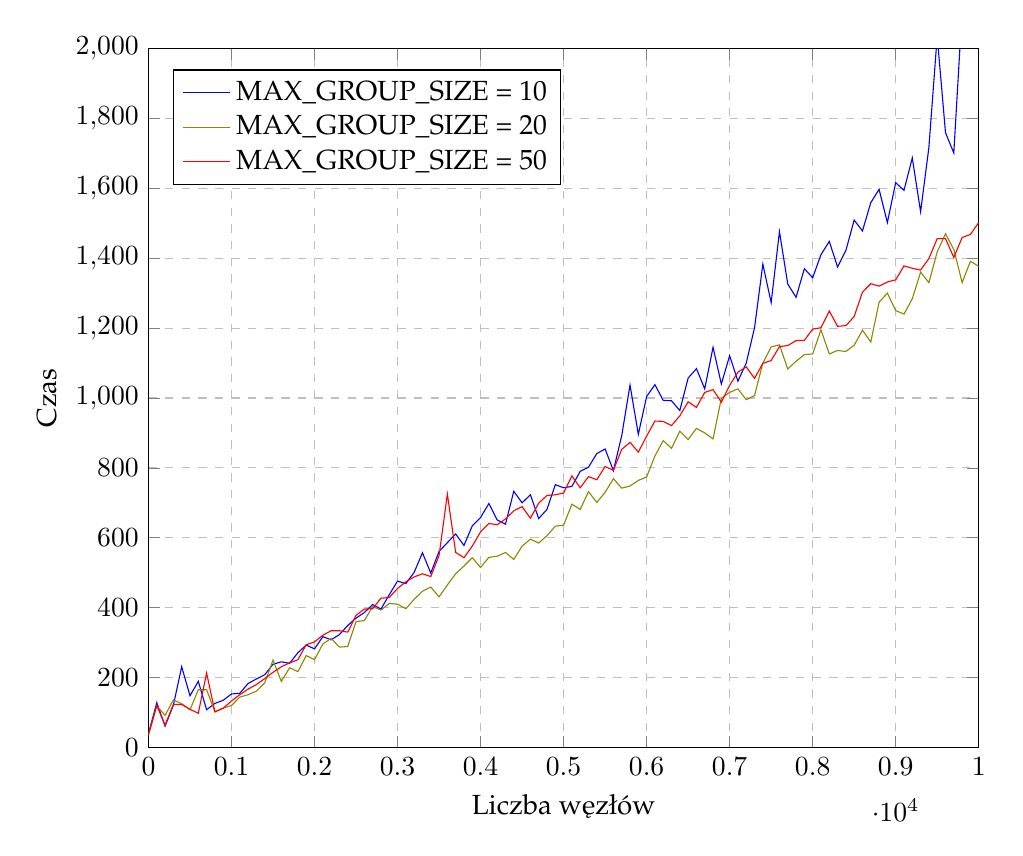
\begin{tikzpicture}
\begin{axis}[
    width=\textwidth,
    xlabel={Liczba węzłów},
    ylabel={Czas},
    xmin=0, xmax=10000,
    ymin=0, ymax=2000,
    legend pos=north west,
    ymajorgrids=true,
    xmajorgrids=true,
    grid style=dashed,
]

\addplot[ color=blue ] coordinates {

(0,40)
(100,128)
(200,61)
(300,121)
(400,231)
(500,148)
(600,189)
(700,108)
(800,126)
(900,135)
(1000,153)
(1100,155)
(1200,183)
(1300,196)
(1400,208)
(1500,238)
(1600,245)
(1700,241)
(1800,271)
(1900,293)
(2000,282)
(2100,317)
(2200,308)
(2300,323)
(2400,349)
(2500,370)
(2600,386)
(2700,409)
(2800,396)
(2900,437)
(3000,476)
(3100,469)
(3200,501)
(3300,557)
(3400,499)
(3500,561)
(3600,586)
(3700,611)
(3800,578)
(3900,634)
(4000,658)
(4100,698)
(4200,651)
(4300,639)
(4400,733)
(4500,700)
(4600,723)
(4700,655)
(4800,681)
(4900,752)
(5000,743)
(5100,747)
(5200,790)
(5300,802)
(5400,841)
(5500,854)
(5600,792)
(5700,892)
(5800,1037)
(5900,896)
(6000,1004)
(6100,1038)
(6200,993)
(6300,992)
(6400,964)
(6500,1057)
(6600,1084)
(6700,1026)
(6800,1145)
(6900,1040)
(7000,1121)
(7100,1048)
(7200,1100)
(7300,1201)
(7400,1383)
(7500,1273)
(7600,1476)
(7700,1326)
(7800,1288)
(7900,1370)
(8000,1344)
(8100,1410)
(8200,1448)
(8300,1375)
(8400,1422)
(8500,1509)
(8600,1478)
(8700,1559)
(8800,1597)
(8900,1502)
(9000,1616)
(9100,1594)
(9200,1687)
(9300,1533)
(9400,1717)
(9500,2035)
(9600,1759)
(9700,1701)
(9800,2109)
(9900,2179)


};

\addplot[ color=olive ] coordinates {

(0,35)
(100,119)
(200,92)
(300,136)
(400,125)
(500,108)
(600,165)
(700,165)
(800,102)
(900,113)
(1000,120)
(1100,144)
(1200,151)
(1300,161)
(1400,185)
(1500,250)
(1600,189)
(1700,228)
(1800,217)
(1900,263)
(2000,251)
(2100,296)
(2200,312)
(2300,287)
(2400,289)
(2500,360)
(2600,363)
(2700,403)
(2800,393)
(2900,412)
(3000,410)
(3100,397)
(3200,424)
(3300,447)
(3400,459)
(3500,431)
(3600,465)
(3700,497)
(3800,519)
(3900,543)
(4000,515)
(4100,544)
(4200,547)
(4300,558)
(4400,538)
(4500,576)
(4600,596)
(4700,585)
(4800,606)
(4900,633)
(5000,636)
(5100,696)
(5200,681)
(5300,732)
(5400,701)
(5500,730)
(5600,769)
(5700,742)
(5800,748)
(5900,764)
(6000,774)
(6100,834)
(6200,878)
(6300,856)
(6400,905)
(6500,881)
(6600,913)
(6700,900)
(6800,883)
(6900,999)
(7000,1016)
(7100,1026)
(7200,995)
(7300,1007)
(7400,1100)
(7500,1146)
(7600,1152)
(7700,1083)
(7800,1105)
(7900,1124)
(8000,1126)
(8100,1195)
(8200,1126)
(8300,1136)
(8400,1133)
(8500,1151)
(8600,1194)
(8700,1160)
(8800,1274)
(8900,1300)
(9000,1250)
(9100,1240)
(9200,1284)
(9300,1360)
(9400,1330)
(9500,1418)
(9600,1470)
(9700,1425)
(9800,1330)
(9900,1391)
(10000,1377)

};

\addplot[ color=red ] coordinates {

(0,38)
(100,120)
(200,64)
(300,123)
(400,123)
(500,109)
(600,98)
(700,213)
(800,102)
(900,112)
(1000,133)
(1100,151)
(1200,167)
(1300,180)
(1400,197)
(1500,215)
(1600,231)
(1700,242)
(1800,251)
(1900,294)
(2000,302)
(2100,321)
(2200,334)
(2300,334)
(2400,330)
(2500,378)
(2600,396)
(2700,397)
(2800,427)
(2900,429)
(3000,455)
(3100,474)
(3200,488)
(3300,497)
(3400,489)
(3500,549)
(3600,725)
(3700,558)
(3800,543)
(3900,576)
(4000,617)
(4100,641)
(4200,637)
(4300,654)
(4400,677)
(4500,689)
(4600,656)
(4700,699)
(4800,721)
(4900,723)
(5000,728)
(5100,777)
(5200,743)
(5300,775)
(5400,766)
(5500,804)
(5600,793)
(5700,853)
(5800,873)
(5900,845)
(6000,891)
(6100,934)
(6200,933)
(6300,921)
(6400,949)
(6500,989)
(6600,973)
(6700,1016)
(6800,1024)
(6900,988)
(7000,1036)
(7100,1074)
(7200,1089)
(7300,1056)
(7400,1099)
(7500,1107)
(7600,1147)
(7700,1150)
(7800,1164)
(7900,1165)
(8000,1197)
(8100,1201)
(8200,1249)
(8300,1205)
(8400,1207)
(8500,1233)
(8600,1303)
(8700,1327)
(8800,1320)
(8900,1332)
(9000,1338)
(9100,1378)
(9200,1371)
(9300,1366)
(9400,1399)
(9500,1456)
(9600,1456)
(9700,1402)
(9800,1459)
(9900,1468)
(10000,1502)



};



\legend{MAX\_GROUP\_SIZE = 10, MAX\_GROUP\_SIZE = 20, MAX\_GROUP\_SIZE = 50}

\end{axis}
\end{tikzpicture}


\caption{Wykres x.y: Czas potrzebny na obsłużenie zmian w sieci w stosunku do liczby węzłów.}
\end{figure}

\end{comment}


\begin{comment}
\begin{figure}[H]
\floatstyle{boxed}
\centering
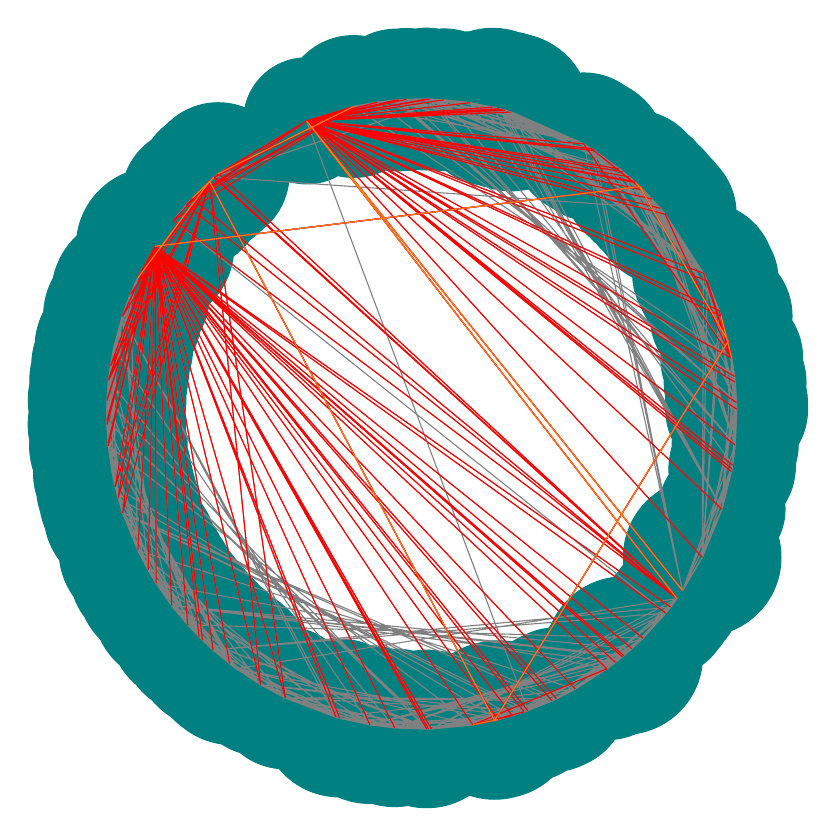
\begin{tikzpicture}
\filldraw[fill=teal, draw=teal]
(-2.82842712474619,-2.8284271247461907) circle (1.0)(2.8110189778289008,-2.845728782980866) circle (0.8)(0.0613568251399524,3.9995293898168502) circle (0.9)(0.09816491409164915,3.998795274784817) circle (0.8)(2.9222510769113104,2.7313821855409923) circle (0.9)(-3.9963109110105814,0.17175302773976286) circle (1.0)(-3.9957651727474275,0.18401272852365938) circle (1.0)(-2.6953160015150237,2.955549297842461) circle (0.9)(-2.972031808540487,-2.6771303533865445) circle (1.0)(2.6679996892145503,-2.980231141765864) circle (0.8)(-2.6404573682696837,3.004660527638744) circle (0.9)(-2.6312267731883154,3.012747196174449) circle (0.9)(0.2820182935584554,3.990045824561214) circle (0.9)(3.0288353860259383,2.6126913718151075) circle (0.9)(-2.5847040519332665,3.052753669053524) circle (0.9)(-0.3431892493777597,-3.985250448731112) circle (1.0)(2.5659240512343326,-3.068555647743281) circle (1.0)(2.5470474449451377,-3.0842420970472544) circle (0.8)(3.0920418134509475,2.537573136654582) circle (0.9)(3.9807389066887877,-0.3920685613182426) circle (0.8)(-3.976961797812752,0.42868969982723365) circle (1.0)(-3.974256542082381,0.4530838087102582) circle (0.9)(2.4609263623225077,-3.153385710506425) circle (0.9)(-3.1759019102173474,-2.4317991398710963) circle (1.0)(0.6111887410337737,3.953030270922998) circle (0.9)(-3.953030270922998,0.6111887410337735) circle (1.0)(2.3531261928905813,-3.2346247263527) circle (0.9)(3.947237607256742,-0.6475455751204471) circle (0.8)(-0.6596524819598796,-3.9452323889783947) circle (1.0)(3.938994007207617,-0.6959354935498548) circle (0.8)(3.932421949724865,-0.7321595518205637) circle (0.30000000000000004)(-3.91070943129804,0.840447347521878) circle (1.0)(-3.372832958567381,-2.150348305182583) circle (1.0)(0.9003356454391713,3.8973575311423034) circle (1.0)(0.9838202013431784,3.877124941426194) circle (0.9)(1.0194626384180583,3.8679058841794083) circle (0.9)(-1.0431764716611025,-3.8615777667907576) circle (1.0)(1.0550187158993254,3.858359173159251) circle (1.0)(-3.4742828238853627,-1.982261047303092) circle (1.0)(1.9502006405937435,-3.4923799136731604) circle (0.8)(-1.0904854217997961,-3.8484856170761663) circle (0.9)(1.1376301488450875,3.8348138995834864) circle (1.0)(3.8132241614167754,-1.2080237972769123) circle (0.8)(-3.801944295797927,1.2430686109984466) circle (1.0)(3.5783979425255303,1.7874753606494973) circle (0.9)(-3.6053953881840877,-1.7323752754126085) circle (1.0)(1.7102203737211281,-3.6159571724937734) circle (0.9)(3.6263828180596613,1.6880010831991992) circle (0.9)(1.6545532489537387,-3.6417651690322685) circle (0.9)(-3.7001969631307103,1.5193888356962044) circle (1.0)(-3.6955181300451465,1.53073372946036) circle (1.0)(-1.4624519912190974,3.723067844315934) circle (0.8)(1.3475594135688813,-3.766176260732083) circle (0.9)(-3.610693272949036,1.7213059253603287) circle (0.9)(-1.7323752754126074,-3.605395388184088) circle (0.9)(3.778419349045921,1.3128393743163707) circle (0.8)(1.301241168649053,-3.7824293015220847) circle (0.8)(-3.7981127223721467,-1.2547269615955658) circle (1.0)(3.801944295797927,1.243068610998446) circle (0.9)(3.561794892979032,-1.820334348505375) circle (1.0)(1.1493898381789185,-3.8313056521101316) circle (0.8)(-3.8551042631817594,-1.0668510298995941) circle (1.0)(-2.045875401751881,-3.437207273428034) circle (0.9)(2.0564109767728866,3.4309144400010885) circle (0.9)(0.9719207196130563,-3.880125012778176) circle (1.0)(-3.8917598088222407,-0.9242324331226838) circle (1.0)(0.9242324331226853,-3.8917598088222403) circle (1.0)(3.8917598088222403,0.9242324331226851) circle (0.1)(-3.3859637550962076,2.1296125115087925) circle (1.0)(2.1503483051825816,3.3728329585673817) circle (0.9)(-0.8644271883048782,3.9054789253200846) circle (0.9)(2.1915762366924008,3.346190908894048) circle (0.9)(3.312180181031023,-2.2426463047893437) circle (0.8)(-3.930157209149765,-0.7442206066537879) circle (1.0)(3.936840369547716,0.7080168816485954) circle (0.9)(0.647545575120447,-3.947237607256742) circle (0.9)(3.241828793010379,-2.3431914298257555) circle (0.8)(-2.3531261928905804,-3.2346247263527004) circle (0.8)(-2.382797217969733,-3.2128301259225798) circle (0.8)(-0.5626329573313968,3.9602328410491885) circle (0.8)(-2.4024659175354746,-3.198149076431621) circle (1.0)(-2.441531225105238,-3.168426309200849) circle (1.0)(3.16092088574924,-2.451240329717639) circle (0.8)(-3.1533857105064245,2.460926362322508) circle (0.1)(3.9714016578394604,0.4774608592439654) circle (0.8)(2.5090072619805763,3.115266049525904) circle (0.8)(-3.9795173231792225,-0.40427945101931195) circle (1.0)(3.9795173231792225,0.4042794510193115) circle (0.9)(3.0998124263794957,-2.528074943759236) circle (0.8)(-3.9830696578706393,-0.3676358259885313) circle (0.9)(2.556497779455103,3.076413350582319) circle (0.8)(-0.33096105819750304,3.9862845831622193) circle (0.8)(-0.318729751885723,3.9872811971646627) circle (0.9)(-0.29425825439866965,3.989161826714761) circle (0.9)(2.6312267731883145,3.01274719617445) circle (0.8)(-2.649663110360687,-2.996545578093837) circle (1.0)(-2.988402423920721,2.658843912813379) circle (0.8)(-0.19627069730967237,3.9951818248206896) circle (0.9)(2.695316001515024,2.9555492978424605) circle (0.9)(2.713400172519446,2.938955512383854) circle (0.8)(3.997289538353398,0.14722889176543597) circle (0.9)(-3.997722418221847,-0.13496468740551104) circle (1.0)(0.12269921270654746,-3.9981176700043726) circle (0.9)(-2.9138575617929003,2.740334671090802) circle (0.9)(0.08589632110187867,-3.999077621404861) circle (0.9)(-3.999077621404861,-0.08589632110187714) circle (0.9)(2.767037033456631,2.8885127757168614) circle (0.1)(3.9995293898168502,0.06135682513995288) circle (0.9)(-2.784708525965852,-2.871480180222927) circle (0.9)(0.06135682513995224,-3.9995293898168502) circle (1.0)(2.811018977828901,2.8457287829808657) circle (0.9);
\draw [gray]
(-2.82842712474619,-2.8284271247461907) -- (-2.972031808540487,-2.6771303533865445)
(-2.82842712474619,-2.8284271247461907) -- (-2.972031808540487,-2.6771303533865445)
(-2.82842712474619,-2.8284271247461907) -- (-2.972031808540487,-2.6771303533865445)
(-2.82842712474619,-2.8284271247461907) -- (-2.972031808540487,-2.6771303533865445)
(-2.82842712474619,-2.8284271247461907) -- (-2.972031808540487,-2.6771303533865445)
(-2.82842712474619,-2.8284271247461907) -- (-3.1759019102173474,-2.4317991398710963)
(-2.82842712474619,-2.8284271247461907) -- (-3.372832958567381,-2.150348305182583)
(-2.82842712474619,-2.8284271247461907) -- (-3.7981127223721467,-1.2547269615955658)
(-2.82842712474619,-2.8284271247461907) -- (-3.9963109110105814,0.17175302773976286)
(-2.82842712474619,-2.8284271247461907) -- (-3.3859637550962076,2.1296125115087925)
(-2.82842712474619,-2.8284271247461907) -- (-3.3859637550962076,2.1296125115087925)
(2.8110189778289008,-2.845728782980866) -- (2.6679996892145503,-2.980231141765864)
(2.8110189778289008,-2.845728782980866) -- (2.6679996892145503,-2.980231141765864)
(2.8110189778289008,-2.845728782980866) -- (2.6679996892145503,-2.980231141765864)
(2.8110189778289008,-2.845728782980866) -- (2.6679996892145503,-2.980231141765864)
(2.8110189778289008,-2.845728782980866) -- (2.6679996892145503,-2.980231141765864)
(2.8110189778289008,-2.845728782980866) -- (2.4609263623225077,-3.153385710506425)
(2.8110189778289008,-2.845728782980866) -- (1.9502006405937435,-3.4923799136731604)
(2.8110189778289008,-2.845728782980866) -- (1.3475594135688813,-3.766176260732083)
(2.8110189778289008,-2.845728782980866) -- (-0.3431892493777597,-3.985250448731112)
(2.8110189778289008,-2.845728782980866) -- (-2.972031808540487,-2.6771303533865445)
(2.8110189778289008,-2.845728782980866) -- (-3.3859637550962076,2.1296125115087925)
(0.0613568251399524,3.9995293898168502) -- (0.09816491409164915,3.998795274784817)
(0.0613568251399524,3.9995293898168502) -- (0.09816491409164915,3.998795274784817)
(0.0613568251399524,3.9995293898168502) -- (0.2820182935584554,3.990045824561214)
(0.0613568251399524,3.9995293898168502) -- (0.2820182935584554,3.990045824561214)
(0.0613568251399524,3.9995293898168502) -- (0.2820182935584554,3.990045824561214)
(0.0613568251399524,3.9995293898168502) -- (0.6111887410337737,3.953030270922998)
(0.0613568251399524,3.9995293898168502) -- (0.9003356454391713,3.8973575311423034)
(0.0613568251399524,3.9995293898168502) -- (2.0564109767728866,3.4309144400010885)
(0.0613568251399524,3.9995293898168502) -- (2.9222510769113104,2.7313821855409923)
(0.0613568251399524,3.9995293898168502) -- (3.9807389066887877,-0.3920685613182426)
(0.0613568251399524,3.9995293898168502) -- (-1.4624519912190974,3.723067844315934)
(0.09816491409164915,3.998795274784817) -- (0.2820182935584554,3.990045824561214)
(0.09816491409164915,3.998795274784817) -- (0.2820182935584554,3.990045824561214)
(0.09816491409164915,3.998795274784817) -- (0.2820182935584554,3.990045824561214)
(0.09816491409164915,3.998795274784817) -- (0.2820182935584554,3.990045824561214)
(0.09816491409164915,3.998795274784817) -- (0.6111887410337737,3.953030270922998)
(0.09816491409164915,3.998795274784817) -- (0.6111887410337737,3.953030270922998)
(0.09816491409164915,3.998795274784817) -- (0.9003356454391713,3.8973575311423034)
(0.09816491409164915,3.998795274784817) -- (2.0564109767728866,3.4309144400010885)
(0.09816491409164915,3.998795274784817) -- (2.9222510769113104,2.7313821855409923)
(0.09816491409164915,3.998795274784817) -- (3.9807389066887877,-0.3920685613182426)
(0.09816491409164915,3.998795274784817) -- (-1.4624519912190974,3.723067844315934)
(2.9222510769113104,2.7313821855409923) -- (3.0288353860259383,2.6126913718151075)
(2.9222510769113104,2.7313821855409923) -- (3.0288353860259383,2.6126913718151075)
(2.9222510769113104,2.7313821855409923) -- (3.0288353860259383,2.6126913718151075)
(2.9222510769113104,2.7313821855409923) -- (3.0288353860259383,2.6126913718151075)
(2.9222510769113104,2.7313821855409923) -- (3.0920418134509475,2.537573136654582)
(2.9222510769113104,2.7313821855409923) -- (3.5783979425255303,1.7874753606494973)
(2.9222510769113104,2.7313821855409923) -- (3.5783979425255303,1.7874753606494973)
(2.9222510769113104,2.7313821855409923) -- (3.778419349045921,1.3128393743163707)
(2.9222510769113104,2.7313821855409923) -- (3.9807389066887877,-0.3920685613182426)
(2.9222510769113104,2.7313821855409923) -- (-1.4624519912190974,3.723067844315934)
(2.9222510769113104,2.7313821855409923) -- (-1.4624519912190974,3.723067844315934)
(-3.9963109110105814,0.17175302773976286) -- (-3.9957651727474275,0.18401272852365938)
(-3.9963109110105814,0.17175302773976286) -- (-3.976961797812752,0.42868969982723365)
(-3.9963109110105814,0.17175302773976286) -- (-3.976961797812752,0.42868969982723365)
(-3.9963109110105814,0.17175302773976286) -- (-3.976961797812752,0.42868969982723365)
(-3.9963109110105814,0.17175302773976286) -- (-3.976961797812752,0.42868969982723365)
(-3.9963109110105814,0.17175302773976286) -- (-3.953030270922998,0.6111887410337735)
(-3.9963109110105814,0.17175302773976286) -- (-3.801944295797927,1.2430686109984466)
(-3.9963109110105814,0.17175302773976286) -- (-3.610693272949036,1.7213059253603287)
(-3.9963109110105814,0.17175302773976286) -- (-3.3859637550962076,2.1296125115087925)
(-3.9963109110105814,0.17175302773976286) -- (-3.3859637550962076,2.1296125115087925)
(-3.9963109110105814,0.17175302773976286) -- (-3.3859637550962076,2.1296125115087925)
(-3.9957651727474275,0.18401272852365938) -- (-3.976961797812752,0.42868969982723365)
(-3.9957651727474275,0.18401272852365938) -- (-3.976961797812752,0.42868969982723365)
(-3.9957651727474275,0.18401272852365938) -- (-3.976961797812752,0.42868969982723365)
(-3.9957651727474275,0.18401272852365938) -- (-3.976961797812752,0.42868969982723365)
(-3.9957651727474275,0.18401272852365938) -- (-3.976961797812752,0.42868969982723365)
(-3.9957651727474275,0.18401272852365938) -- (-3.953030270922998,0.6111887410337735)
(-3.9957651727474275,0.18401272852365938) -- (-3.801944295797927,1.2430686109984466)
(-3.9957651727474275,0.18401272852365938) -- (-3.610693272949036,1.7213059253603287)
(-3.9957651727474275,0.18401272852365938) -- (-3.3859637550962076,2.1296125115087925)
(-3.9957651727474275,0.18401272852365938) -- (-3.3859637550962076,2.1296125115087925)
(-3.9957651727474275,0.18401272852365938) -- (-3.3859637550962076,2.1296125115087925)
(-2.6953160015150237,2.955549297842461) -- (0.9242324331226853,-3.8917598088222403)
(-2.6953160015150237,2.955549297842461) -- (0.9242324331226853,-3.8917598088222403)
(-2.6953160015150237,2.955549297842461) -- (0.9242324331226853,-3.8917598088222403)
(-2.6953160015150237,2.955549297842461) -- (0.9242324331226853,-3.8917598088222403)
(-2.6953160015150237,2.955549297842461) -- (0.9242324331226853,-3.8917598088222403)
(-2.6953160015150237,2.955549297842461) -- (0.9242324331226853,-3.8917598088222403)
(-2.6953160015150237,2.955549297842461) -- (0.9242324331226853,-3.8917598088222403)
(-2.6953160015150237,2.955549297842461) -- (0.9242324331226853,-3.8917598088222403)
(-2.6953160015150237,2.955549297842461) -- (0.9242324331226853,-3.8917598088222403)
(-2.6953160015150237,2.955549297842461) -- (0.9242324331226853,-3.8917598088222403)
(-2.6953160015150237,2.955549297842461) -- (0.9242324331226853,-3.8917598088222403)
(-2.972031808540487,-2.6771303533865445) -- (-3.1759019102173474,-2.4317991398710963)
(-2.972031808540487,-2.6771303533865445) -- (-3.1759019102173474,-2.4317991398710963)
(-2.972031808540487,-2.6771303533865445) -- (-3.1759019102173474,-2.4317991398710963)
(-2.972031808540487,-2.6771303533865445) -- (-3.1759019102173474,-2.4317991398710963)
(-2.972031808540487,-2.6771303533865445) -- (-3.1759019102173474,-2.4317991398710963)
(-2.972031808540487,-2.6771303533865445) -- (-3.372832958567381,-2.150348305182583)
(-2.972031808540487,-2.6771303533865445) -- (-3.4742828238853627,-1.982261047303092)
(-2.972031808540487,-2.6771303533865445) -- (-3.7981127223721467,-1.2547269615955658)
(-2.972031808540487,-2.6771303533865445) -- (-3.976961797812752,0.42868969982723365)
(-2.972031808540487,-2.6771303533865445) -- (-3.3859637550962076,2.1296125115087925)
(-2.972031808540487,-2.6771303533865445) -- (-3.3859637550962076,2.1296125115087925)
(2.6679996892145503,-2.980231141765864) -- (2.5659240512343326,-3.068555647743281)
(2.6679996892145503,-2.980231141765864) -- (2.5659240512343326,-3.068555647743281)
(2.6679996892145503,-2.980231141765864) -- (2.5659240512343326,-3.068555647743281)
(2.6679996892145503,-2.980231141765864) -- (2.5659240512343326,-3.068555647743281)
(2.6679996892145503,-2.980231141765864) -- (2.4609263623225077,-3.153385710506425)
(2.6679996892145503,-2.980231141765864) -- (2.3531261928905813,-3.2346247263527)
(2.6679996892145503,-2.980231141765864) -- (1.9502006405937435,-3.4923799136731604)
(2.6679996892145503,-2.980231141765864) -- (1.301241168649053,-3.7824293015220847)
(2.6679996892145503,-2.980231141765864) -- (-0.3431892493777597,-3.985250448731112)
(2.6679996892145503,-2.980231141765864) -- (-3.1759019102173474,-2.4317991398710963)
(2.6679996892145503,-2.980231141765864) -- (-3.3859637550962076,2.1296125115087925)
(-2.6404573682696837,3.004660527638744) -- (-2.6312267731883154,3.012747196174449)
(-2.6404573682696837,3.004660527638744) -- (-2.5847040519332665,3.052753669053524)
(-2.6404573682696837,3.004660527638744) -- (-2.5847040519332665,3.052753669053524)
(-2.6404573682696837,3.004660527638744) -- (-0.8644271883048782,3.9054789253200846)
(-2.6404573682696837,3.004660527638744) -- (-0.8644271883048782,3.9054789253200846)
(-2.6404573682696837,3.004660527638744) -- (-0.8644271883048782,3.9054789253200846)
(-2.6404573682696837,3.004660527638744) -- (-0.8644271883048782,3.9054789253200846)
(-2.6404573682696837,3.004660527638744) -- (3.241828793010379,-2.3431914298257555)
(-2.6404573682696837,3.004660527638744) -- (3.241828793010379,-2.3431914298257555)
(-2.6404573682696837,3.004660527638744) -- (3.241828793010379,-2.3431914298257555)
(-2.6404573682696837,3.004660527638744) -- (-1.4624519912190974,3.723067844315934)
(-2.6312267731883154,3.012747196174449) -- (-2.5847040519332665,3.052753669053524)
(-2.6312267731883154,3.012747196174449) -- (-2.5847040519332665,3.052753669053524)
(-2.6312267731883154,3.012747196174449) -- (-2.5847040519332665,3.052753669053524)
(-2.6312267731883154,3.012747196174449) -- (-0.8644271883048782,3.9054789253200846)
(-2.6312267731883154,3.012747196174449) -- (-0.8644271883048782,3.9054789253200846)
(-2.6312267731883154,3.012747196174449) -- (-0.8644271883048782,3.9054789253200846)
(-2.6312267731883154,3.012747196174449) -- (-0.8644271883048782,3.9054789253200846)
(-2.6312267731883154,3.012747196174449) -- (3.241828793010379,-2.3431914298257555)
(-2.6312267731883154,3.012747196174449) -- (0.2820182935584554,3.990045824561214)
(-2.6312267731883154,3.012747196174449) -- (3.0288353860259383,2.6126913718151075)
(-2.6312267731883154,3.012747196174449) -- (-1.4624519912190974,3.723067844315934)
(0.2820182935584554,3.990045824561214) -- (0.6111887410337737,3.953030270922998)
(0.2820182935584554,3.990045824561214) -- (0.6111887410337737,3.953030270922998)
(0.2820182935584554,3.990045824561214) -- (0.6111887410337737,3.953030270922998)
(0.2820182935584554,3.990045824561214) -- (0.6111887410337737,3.953030270922998)
(0.2820182935584554,3.990045824561214) -- (0.6111887410337737,3.953030270922998)
(0.2820182935584554,3.990045824561214) -- (0.9003356454391713,3.8973575311423034)
(0.2820182935584554,3.990045824561214) -- (1.0550187158993254,3.858359173159251)
(0.2820182935584554,3.990045824561214) -- (2.0564109767728866,3.4309144400010885)
(0.2820182935584554,3.990045824561214) -- (3.0288353860259383,2.6126913718151075)
(0.2820182935584554,3.990045824561214) -- (3.9807389066887877,-0.3920685613182426)
(0.2820182935584554,3.990045824561214) -- (-1.4624519912190974,3.723067844315934)
(3.0288353860259383,2.6126913718151075) -- (3.0920418134509475,2.537573136654582)
(3.0288353860259383,2.6126913718151075) -- (3.0920418134509475,2.537573136654582)
(3.0288353860259383,2.6126913718151075) -- (3.0920418134509475,2.537573136654582)
(3.0288353860259383,2.6126913718151075) -- (3.0920418134509475,2.537573136654582)
(3.0288353860259383,2.6126913718151075) -- (3.5783979425255303,1.7874753606494973)
(3.0288353860259383,2.6126913718151075) -- (3.5783979425255303,1.7874753606494973)
(3.0288353860259383,2.6126913718151075) -- (3.5783979425255303,1.7874753606494973)
(3.0288353860259383,2.6126913718151075) -- (3.801944295797927,1.243068610998446)
(3.0288353860259383,2.6126913718151075) -- (3.9807389066887877,-0.3920685613182426)
(3.0288353860259383,2.6126913718151075) -- (-1.4624519912190974,3.723067844315934)
(3.0288353860259383,2.6126913718151075) -- (-1.4624519912190974,3.723067844315934)
(-2.5847040519332665,3.052753669053524) -- (-0.8644271883048782,3.9054789253200846)
(-2.5847040519332665,3.052753669053524) -- (-0.8644271883048782,3.9054789253200846)
(-2.5847040519332665,3.052753669053524) -- (-0.8644271883048782,3.9054789253200846)
(-2.5847040519332665,3.052753669053524) -- (-0.8644271883048782,3.9054789253200846)
(-2.5847040519332665,3.052753669053524) -- (-0.8644271883048782,3.9054789253200846)
(-2.5847040519332665,3.052753669053524) -- (-0.8644271883048782,3.9054789253200846)
(-2.5847040519332665,3.052753669053524) -- (-0.8644271883048782,3.9054789253200846)
(-2.5847040519332665,3.052753669053524) -- (-0.8644271883048782,3.9054789253200846)
(-2.5847040519332665,3.052753669053524) -- (3.241828793010379,-2.3431914298257555)
(-2.5847040519332665,3.052753669053524) -- (3.241828793010379,-2.3431914298257555)
(-2.5847040519332665,3.052753669053524) -- (-1.4624519912190974,3.723067844315934)
(-0.3431892493777597,-3.985250448731112) -- (-0.6596524819598796,-3.9452323889783947)
(-0.3431892493777597,-3.985250448731112) -- (-0.6596524819598796,-3.9452323889783947)
(-0.3431892493777597,-3.985250448731112) -- (-0.6596524819598796,-3.9452323889783947)
(-0.3431892493777597,-3.985250448731112) -- (-0.6596524819598796,-3.9452323889783947)
(-0.3431892493777597,-3.985250448731112) -- (-0.6596524819598796,-3.9452323889783947)
(-0.3431892493777597,-3.985250448731112) -- (-1.0431764716611025,-3.8615777667907576)
(-0.3431892493777597,-3.985250448731112) -- (-1.7323752754126074,-3.605395388184088)
(-0.3431892493777597,-3.985250448731112) -- (-2.045875401751881,-3.437207273428034)
(-0.3431892493777597,-3.985250448731112) -- (-3.1759019102173474,-2.4317991398710963)
(-0.3431892493777597,-3.985250448731112) -- (-3.976961797812752,0.42868969982723365)
(-0.3431892493777597,-3.985250448731112) -- (-3.3859637550962076,2.1296125115087925)
(2.5659240512343326,-3.068555647743281) -- (2.5470474449451377,-3.0842420970472544)
(2.5659240512343326,-3.068555647743281) -- (2.5470474449451377,-3.0842420970472544)
(2.5659240512343326,-3.068555647743281) -- (2.4609263623225077,-3.153385710506425)
(2.5659240512343326,-3.068555647743281) -- (2.4609263623225077,-3.153385710506425)
(2.5659240512343326,-3.068555647743281) -- (2.3531261928905813,-3.2346247263527)
(2.5659240512343326,-3.068555647743281) -- (1.9502006405937435,-3.4923799136731604)
(2.5659240512343326,-3.068555647743281) -- (1.7102203737211281,-3.6159571724937734)
(2.5659240512343326,-3.068555647743281) -- (1.1493898381789185,-3.8313056521101316)
(2.5659240512343326,-3.068555647743281) -- (-0.6596524819598796,-3.9452323889783947)
(2.5659240512343326,-3.068555647743281) -- (-3.1759019102173474,-2.4317991398710963)
(2.5659240512343326,-3.068555647743281) -- (-3.3859637550962076,2.1296125115087925)
(2.5470474449451377,-3.0842420970472544) -- (2.4609263623225077,-3.153385710506425)
(2.5470474449451377,-3.0842420970472544) -- (2.4609263623225077,-3.153385710506425)
(2.5470474449451377,-3.0842420970472544) -- (2.4609263623225077,-3.153385710506425)
(2.5470474449451377,-3.0842420970472544) -- (2.4609263623225077,-3.153385710506425)
(2.5470474449451377,-3.0842420970472544) -- (2.3531261928905813,-3.2346247263527)
(2.5470474449451377,-3.0842420970472544) -- (1.9502006405937435,-3.4923799136731604)
(2.5470474449451377,-3.0842420970472544) -- (1.7102203737211281,-3.6159571724937734)
(2.5470474449451377,-3.0842420970472544) -- (1.1493898381789185,-3.8313056521101316)
(2.5470474449451377,-3.0842420970472544) -- (-0.6596524819598796,-3.9452323889783947)
(2.5470474449451377,-3.0842420970472544) -- (-3.1759019102173474,-2.4317991398710963)
(2.5470474449451377,-3.0842420970472544) -- (-3.3859637550962076,2.1296125115087925)
(3.0920418134509475,2.537573136654582) -- (3.5783979425255303,1.7874753606494973)
(3.0920418134509475,2.537573136654582) -- (3.5783979425255303,1.7874753606494973)
(3.0920418134509475,2.537573136654582) -- (3.5783979425255303,1.7874753606494973)
(3.0920418134509475,2.537573136654582) -- (3.5783979425255303,1.7874753606494973)
(3.0920418134509475,2.537573136654582) -- (3.5783979425255303,1.7874753606494973)
(3.0920418134509475,2.537573136654582) -- (3.5783979425255303,1.7874753606494973)
(3.0920418134509475,2.537573136654582) -- (3.5783979425255303,1.7874753606494973)
(3.0920418134509475,2.537573136654582) -- (3.936840369547716,0.7080168816485954)
(3.0920418134509475,2.537573136654582) -- (3.9807389066887877,-0.3920685613182426)
(3.0920418134509475,2.537573136654582) -- (-1.4624519912190974,3.723067844315934)
(3.0920418134509475,2.537573136654582) -- (-1.4624519912190974,3.723067844315934)
(3.9807389066887877,-0.3920685613182426) -- (3.947237607256742,-0.6475455751204471)
(3.9807389066887877,-0.3920685613182426) -- (3.947237607256742,-0.6475455751204471)
(3.9807389066887877,-0.3920685613182426) -- (3.947237607256742,-0.6475455751204471)
(3.9807389066887877,-0.3920685613182426) -- (3.947237607256742,-0.6475455751204471)
(3.9807389066887877,-0.3920685613182426) -- (3.947237607256742,-0.6475455751204471)
(3.9807389066887877,-0.3920685613182426) -- (3.8132241614167754,-1.2080237972769123)
(3.9807389066887877,-0.3920685613182426) -- (3.8132241614167754,-1.2080237972769123)
(3.9807389066887877,-0.3920685613182426) -- (3.312180181031023,-2.2426463047893437)
(3.9807389066887877,-0.3920685613182426) -- (-1.4624519912190974,3.723067844315934)
(3.9807389066887877,-0.3920685613182426) -- (-1.4624519912190974,3.723067844315934)
(3.9807389066887877,-0.3920685613182426) -- (-1.4624519912190974,3.723067844315934)
(-3.976961797812752,0.42868969982723365) -- (-3.974256542082381,0.4530838087102582)
(-3.976961797812752,0.42868969982723365) -- (-3.974256542082381,0.4530838087102582)
(-3.976961797812752,0.42868969982723365) -- (-3.953030270922998,0.6111887410337735)
(-3.976961797812752,0.42868969982723365) -- (-3.953030270922998,0.6111887410337735)
(-3.976961797812752,0.42868969982723365) -- (-3.91070943129804,0.840447347521878)
(-3.976961797812752,0.42868969982723365) -- (-3.91070943129804,0.840447347521878)
(-3.976961797812752,0.42868969982723365) -- (-3.801944295797927,1.2430686109984466)
(-3.976961797812752,0.42868969982723365) -- (-2.6953160015150237,2.955549297842461)
(-3.976961797812752,0.42868969982723365) -- (-3.3859637550962076,2.1296125115087925)
(-3.976961797812752,0.42868969982723365) -- (-3.3859637550962076,2.1296125115087925)
(-3.976961797812752,0.42868969982723365) -- (-3.3859637550962076,2.1296125115087925)
(-3.974256542082381,0.4530838087102582) -- (-3.953030270922998,0.6111887410337735)
(-3.974256542082381,0.4530838087102582) -- (-3.953030270922998,0.6111887410337735)
(-3.974256542082381,0.4530838087102582) -- (-3.953030270922998,0.6111887410337735)
(-3.974256542082381,0.4530838087102582) -- (-3.953030270922998,0.6111887410337735)
(-3.974256542082381,0.4530838087102582) -- (-3.91070943129804,0.840447347521878)
(-3.974256542082381,0.4530838087102582) -- (-3.91070943129804,0.840447347521878)
(-3.974256542082381,0.4530838087102582) -- (-3.801944295797927,1.2430686109984466)
(-3.974256542082381,0.4530838087102582) -- (-2.6953160015150237,2.955549297842461)
(-3.974256542082381,0.4530838087102582) -- (-3.3859637550962076,2.1296125115087925)
(-3.974256542082381,0.4530838087102582) -- (-3.3859637550962076,2.1296125115087925)
(-3.974256542082381,0.4530838087102582) -- (-3.3859637550962076,2.1296125115087925)
(2.4609263623225077,-3.153385710506425) -- (2.3531261928905813,-3.2346247263527)
(2.4609263623225077,-3.153385710506425) -- (2.3531261928905813,-3.2346247263527)
(2.4609263623225077,-3.153385710506425) -- (2.3531261928905813,-3.2346247263527)
(2.4609263623225077,-3.153385710506425) -- (2.3531261928905813,-3.2346247263527)
(2.4609263623225077,-3.153385710506425) -- (1.9502006405937435,-3.4923799136731604)
(2.4609263623225077,-3.153385710506425) -- (1.9502006405937435,-3.4923799136731604)
(2.4609263623225077,-3.153385710506425) -- (1.7102203737211281,-3.6159571724937734)
(2.4609263623225077,-3.153385710506425) -- (0.9719207196130563,-3.880125012778176)
(2.4609263623225077,-3.153385710506425) -- (-0.6596524819598796,-3.9452323889783947)
(2.4609263623225077,-3.153385710506425) -- (-3.1759019102173474,-2.4317991398710963)
(2.4609263623225077,-3.153385710506425) -- (-3.3859637550962076,2.1296125115087925)
(-3.1759019102173474,-2.4317991398710963) -- (-3.372832958567381,-2.150348305182583)
(-3.1759019102173474,-2.4317991398710963) -- (-3.372832958567381,-2.150348305182583)
(-3.1759019102173474,-2.4317991398710963) -- (-3.372832958567381,-2.150348305182583)
(-3.1759019102173474,-2.4317991398710963) -- (-3.372832958567381,-2.150348305182583)
(-3.1759019102173474,-2.4317991398710963) -- (-3.372832958567381,-2.150348305182583)
(-3.1759019102173474,-2.4317991398710963) -- (-3.4742828238853627,-1.982261047303092)
(-3.1759019102173474,-2.4317991398710963) -- (-3.6053953881840877,-1.7323752754126085)
(-3.1759019102173474,-2.4317991398710963) -- (-3.8917598088222407,-0.9242324331226838)
(-3.1759019102173474,-2.4317991398710963) -- (-3.953030270922998,0.6111887410337735)
(-3.1759019102173474,-2.4317991398710963) -- (-3.3859637550962076,2.1296125115087925)
(-3.1759019102173474,-2.4317991398710963) -- (-3.3859637550962076,2.1296125115087925)
(0.6111887410337737,3.953030270922998) -- (0.9003356454391713,3.8973575311423034)
(0.6111887410337737,3.953030270922998) -- (0.9003356454391713,3.8973575311423034)
(0.6111887410337737,3.953030270922998) -- (0.9003356454391713,3.8973575311423034)
(0.6111887410337737,3.953030270922998) -- (0.9003356454391713,3.8973575311423034)
(0.6111887410337737,3.953030270922998) -- (0.9003356454391713,3.8973575311423034)
(0.6111887410337737,3.953030270922998) -- (1.0194626384180583,3.8679058841794083)
(0.6111887410337737,3.953030270922998) -- (2.0564109767728866,3.4309144400010885)
(0.6111887410337737,3.953030270922998) -- (2.1503483051825816,3.3728329585673817)
(0.6111887410337737,3.953030270922998) -- (3.5783979425255303,1.7874753606494973)
(0.6111887410337737,3.953030270922998) -- (3.947237607256742,-0.6475455751204471)
(0.6111887410337737,3.953030270922998) -- (-1.4624519912190974,3.723067844315934)
(-3.953030270922998,0.6111887410337735) -- (-3.91070943129804,0.840447347521878)
(-3.953030270922998,0.6111887410337735) -- (-3.91070943129804,0.840447347521878)
(-3.953030270922998,0.6111887410337735) -- (-3.91070943129804,0.840447347521878)
(-3.953030270922998,0.6111887410337735) -- (-3.91070943129804,0.840447347521878)
(-3.953030270922998,0.6111887410337735) -- (-3.91070943129804,0.840447347521878)
(-3.953030270922998,0.6111887410337735) -- (-3.801944295797927,1.2430686109984466)
(-3.953030270922998,0.6111887410337735) -- (-3.7001969631307103,1.5193888356962044)
(-3.953030270922998,0.6111887410337735) -- (-2.6953160015150237,2.955549297842461)
(-3.953030270922998,0.6111887410337735) -- (-3.3859637550962076,2.1296125115087925)
(-3.953030270922998,0.6111887410337735) -- (-3.3859637550962076,2.1296125115087925)
(-3.953030270922998,0.6111887410337735) -- (-3.3859637550962076,2.1296125115087925)
(2.3531261928905813,-3.2346247263527) -- (1.9502006405937435,-3.4923799136731604)
(2.3531261928905813,-3.2346247263527) -- (1.9502006405937435,-3.4923799136731604)
(2.3531261928905813,-3.2346247263527) -- (1.9502006405937435,-3.4923799136731604)
(2.3531261928905813,-3.2346247263527) -- (1.9502006405937435,-3.4923799136731604)
(2.3531261928905813,-3.2346247263527) -- (1.9502006405937435,-3.4923799136731604)
(2.3531261928905813,-3.2346247263527) -- (1.9502006405937435,-3.4923799136731604)
(2.3531261928905813,-3.2346247263527) -- (1.6545532489537387,-3.6417651690322685)
(2.3531261928905813,-3.2346247263527) -- (0.647545575120447,-3.947237607256742)
(2.3531261928905813,-3.2346247263527) -- (-0.6596524819598796,-3.9452323889783947)
(2.3531261928905813,-3.2346247263527) -- (-3.372832958567381,-2.150348305182583)
(2.3531261928905813,-3.2346247263527) -- (-3.3859637550962076,2.1296125115087925)
(3.947237607256742,-0.6475455751204471) -- (3.938994007207617,-0.6959354935498548)
(3.947237607256742,-0.6475455751204471) -- (3.938994007207617,-0.6959354935498548)
(3.947237607256742,-0.6475455751204471) -- (3.938994007207617,-0.6959354935498548)
(3.947237607256742,-0.6475455751204471) -- (3.8132241614167754,-1.2080237972769123)
(3.947237607256742,-0.6475455751204471) -- (3.8132241614167754,-1.2080237972769123)
(3.947237607256742,-0.6475455751204471) -- (3.8132241614167754,-1.2080237972769123)
(3.947237607256742,-0.6475455751204471) -- (3.561794892979032,-1.820334348505375)
(3.947237607256742,-0.6475455751204471) -- (3.312180181031023,-2.2426463047893437)
(3.947237607256742,-0.6475455751204471) -- (-1.4624519912190974,3.723067844315934)
(3.947237607256742,-0.6475455751204471) -- (-1.4624519912190974,3.723067844315934)
(3.947237607256742,-0.6475455751204471) -- (-1.4624519912190974,3.723067844315934)
(-0.6596524819598796,-3.9452323889783947) -- (-1.0431764716611025,-3.8615777667907576)
(-0.6596524819598796,-3.9452323889783947) -- (-1.0431764716611025,-3.8615777667907576)
(-0.6596524819598796,-3.9452323889783947) -- (-1.0431764716611025,-3.8615777667907576)
(-0.6596524819598796,-3.9452323889783947) -- (-1.0431764716611025,-3.8615777667907576)
(-0.6596524819598796,-3.9452323889783947) -- (-1.0431764716611025,-3.8615777667907576)
(-0.6596524819598796,-3.9452323889783947) -- (-1.0431764716611025,-3.8615777667907576)
(-0.6596524819598796,-3.9452323889783947) -- (-1.7323752754126074,-3.605395388184088)
(-0.6596524819598796,-3.9452323889783947) -- (-2.3531261928905804,-3.2346247263527004)
(-0.6596524819598796,-3.9452323889783947) -- (-3.372832958567381,-2.150348305182583)
(-0.6596524819598796,-3.9452323889783947) -- (-3.91070943129804,0.840447347521878)
(-0.6596524819598796,-3.9452323889783947) -- (-3.3859637550962076,2.1296125115087925)
(3.938994007207617,-0.6959354935498548) -- (3.932421949724865,-0.7321595518205637)
(3.938994007207617,-0.6959354935498548) -- (3.932421949724865,-0.7321595518205637)
(3.938994007207617,-0.6959354935498548) -- (3.8132241614167754,-1.2080237972769123)
(3.938994007207617,-0.6959354935498548) -- (3.8132241614167754,-1.2080237972769123)
(3.938994007207617,-0.6959354935498548) -- (3.8132241614167754,-1.2080237972769123)
(3.938994007207617,-0.6959354935498548) -- (3.8132241614167754,-1.2080237972769123)
(3.938994007207617,-0.6959354935498548) -- (3.561794892979032,-1.820334348505375)
(3.938994007207617,-0.6959354935498548) -- (3.312180181031023,-2.2426463047893437)
(3.938994007207617,-0.6959354935498548) -- (-1.4624519912190974,3.723067844315934)
(3.938994007207617,-0.6959354935498548) -- (-1.4624519912190974,3.723067844315934)
(3.938994007207617,-0.6959354935498548) -- (-1.4624519912190974,3.723067844315934)
(3.932421949724865,-0.7321595518205637) -- (3.8132241614167754,-1.2080237972769123)
(3.932421949724865,-0.7321595518205637) -- (3.8132241614167754,-1.2080237972769123)
(3.932421949724865,-0.7321595518205637) -- (3.8132241614167754,-1.2080237972769123)
(3.932421949724865,-0.7321595518205637) -- (3.8132241614167754,-1.2080237972769123)
(3.932421949724865,-0.7321595518205637) -- (3.8132241614167754,-1.2080237972769123)
(3.932421949724865,-0.7321595518205637) -- (3.8132241614167754,-1.2080237972769123)
(3.932421949724865,-0.7321595518205637) -- (3.561794892979032,-1.820334348505375)
(3.932421949724865,-0.7321595518205637) -- (3.312180181031023,-2.2426463047893437)
(3.932421949724865,-0.7321595518205637) -- (-1.4624519912190974,3.723067844315934)
(3.932421949724865,-0.7321595518205637) -- (-1.4624519912190974,3.723067844315934)
(3.932421949724865,-0.7321595518205637) -- (-1.4624519912190974,3.723067844315934)
(-3.91070943129804,0.840447347521878) -- (-3.801944295797927,1.2430686109984466)
(-3.91070943129804,0.840447347521878) -- (-3.801944295797927,1.2430686109984466)
(-3.91070943129804,0.840447347521878) -- (-3.801944295797927,1.2430686109984466)
(-3.91070943129804,0.840447347521878) -- (-3.801944295797927,1.2430686109984466)
(-3.91070943129804,0.840447347521878) -- (-3.801944295797927,1.2430686109984466)
(-3.91070943129804,0.840447347521878) -- (-3.801944295797927,1.2430686109984466)
(-3.91070943129804,0.840447347521878) -- (-3.610693272949036,1.7213059253603287)
(-3.372832958567381,-2.150348305182583) -- (-3.4742828238853627,-1.982261047303092)
(-3.372832958567381,-2.150348305182583) -- (-3.4742828238853627,-1.982261047303092)
(-3.372832958567381,-2.150348305182583) -- (-3.4742828238853627,-1.982261047303092)
(-3.372832958567381,-2.150348305182583) -- (-3.4742828238853627,-1.982261047303092)
(-3.372832958567381,-2.150348305182583) -- (-3.4742828238853627,-1.982261047303092)
(-3.372832958567381,-2.150348305182583) -- (-3.6053953881840877,-1.7323752754126085)
(-3.372832958567381,-2.150348305182583) -- (-3.7981127223721467,-1.2547269615955658)
(-3.372832958567381,-2.150348305182583) -- (-3.9795173231792225,-0.40427945101931195)
(-3.372832958567381,-2.150348305182583) -- (-3.801944295797927,1.2430686109984466)
(-3.372832958567381,-2.150348305182583) -- (-3.3859637550962076,2.1296125115087925)
(-3.372832958567381,-2.150348305182583) -- (-3.3859637550962076,2.1296125115087925)
(0.9003356454391713,3.8973575311423034) -- (0.9838202013431784,3.877124941426194)
(0.9003356454391713,3.8973575311423034) -- (0.9838202013431784,3.877124941426194)
(0.9003356454391713,3.8973575311423034) -- (0.9838202013431784,3.877124941426194)
(0.9003356454391713,3.8973575311423034) -- (1.0194626384180583,3.8679058841794083)
(0.9003356454391713,3.8973575311423034) -- (1.1376301488450875,3.8348138995834864)
(0.9003356454391713,3.8973575311423034) -- (2.0564109767728866,3.4309144400010885)
(0.9003356454391713,3.8973575311423034) -- (2.0564109767728866,3.4309144400010885)
(0.9003356454391713,3.8973575311423034) -- (2.5090072619805763,3.115266049525904)
(0.9003356454391713,3.8973575311423034) -- (3.5783979425255303,1.7874753606494973)
(0.9003356454391713,3.8973575311423034) -- (3.8132241614167754,-1.2080237972769123)
(0.9003356454391713,3.8973575311423034) -- (-1.4624519912190974,3.723067844315934)
(0.9838202013431784,3.877124941426194) -- (1.0194626384180583,3.8679058841794083)
(0.9838202013431784,3.877124941426194) -- (1.0194626384180583,3.8679058841794083)
(0.9838202013431784,3.877124941426194) -- (1.0550187158993254,3.858359173159251)
(0.9838202013431784,3.877124941426194) -- (1.1376301488450875,3.8348138995834864)
(0.9838202013431784,3.877124941426194) -- (2.0564109767728866,3.4309144400010885)
(0.9838202013431784,3.877124941426194) -- (2.0564109767728866,3.4309144400010885)
(0.9838202013431784,3.877124941426194) -- (2.0564109767728866,3.4309144400010885)
(0.9838202013431784,3.877124941426194) -- (2.5090072619805763,3.115266049525904)
(0.9838202013431784,3.877124941426194) -- (3.5783979425255303,1.7874753606494973)
(0.9838202013431784,3.877124941426194) -- (3.8132241614167754,-1.2080237972769123)
(0.9838202013431784,3.877124941426194) -- (-1.4624519912190974,3.723067844315934)
(1.0194626384180583,3.8679058841794083) -- (1.0550187158993254,3.858359173159251)
(1.0194626384180583,3.8679058841794083) -- (1.0550187158993254,3.858359173159251)
(1.0194626384180583,3.8679058841794083) -- (1.1376301488450875,3.8348138995834864)
(1.0194626384180583,3.8679058841794083) -- (1.1376301488450875,3.8348138995834864)
(1.0194626384180583,3.8679058841794083) -- (2.0564109767728866,3.4309144400010885)
(1.0194626384180583,3.8679058841794083) -- (2.0564109767728866,3.4309144400010885)
(1.0194626384180583,3.8679058841794083) -- (2.0564109767728866,3.4309144400010885)
(1.0194626384180583,3.8679058841794083) -- (2.5090072619805763,3.115266049525904)
(1.0194626384180583,3.8679058841794083) -- (3.5783979425255303,1.7874753606494973)
(1.0194626384180583,3.8679058841794083) -- (3.8132241614167754,-1.2080237972769123)
(1.0194626384180583,3.8679058841794083) -- (-1.4624519912190974,3.723067844315934)
(-1.0431764716611025,-3.8615777667907576) -- (-1.0904854217997961,-3.8484856170761663)
(-1.0431764716611025,-3.8615777667907576) -- (-1.0904854217997961,-3.8484856170761663)
(-1.0431764716611025,-3.8615777667907576) -- (-1.0904854217997961,-3.8484856170761663)
(-1.0431764716611025,-3.8615777667907576) -- (-1.7323752754126074,-3.605395388184088)
(-1.0431764716611025,-3.8615777667907576) -- (-1.7323752754126074,-3.605395388184088)
(-1.0431764716611025,-3.8615777667907576) -- (-1.7323752754126074,-3.605395388184088)
(-1.0431764716611025,-3.8615777667907576) -- (-2.045875401751881,-3.437207273428034)
(-1.0431764716611025,-3.8615777667907576) -- (-2.441531225105238,-3.168426309200849)
(-1.0431764716611025,-3.8615777667907576) -- (-3.4742828238853627,-1.982261047303092)
(-1.0431764716611025,-3.8615777667907576) -- (-3.801944295797927,1.2430686109984466)
(-1.0431764716611025,-3.8615777667907576) -- (-3.3859637550962076,2.1296125115087925)
(1.0550187158993254,3.858359173159251) -- (1.1376301488450875,3.8348138995834864)
(1.0550187158993254,3.858359173159251) -- (1.1376301488450875,3.8348138995834864)
(1.0550187158993254,3.858359173159251) -- (1.1376301488450875,3.8348138995834864)
(1.0550187158993254,3.858359173159251) -- (2.0564109767728866,3.4309144400010885)
(1.0550187158993254,3.858359173159251) -- (2.0564109767728866,3.4309144400010885)
(1.0550187158993254,3.858359173159251) -- (2.0564109767728866,3.4309144400010885)
(1.0550187158993254,3.858359173159251) -- (2.0564109767728866,3.4309144400010885)
(1.0550187158993254,3.858359173159251) -- (2.5090072619805763,3.115266049525904)
(1.0550187158993254,3.858359173159251) -- (3.5783979425255303,1.7874753606494973)
(1.0550187158993254,3.858359173159251) -- (3.8132241614167754,-1.2080237972769123)
(1.0550187158993254,3.858359173159251) -- (-1.4624519912190974,3.723067844315934)
(-3.4742828238853627,-1.982261047303092) -- (-3.6053953881840877,-1.7323752754126085)
(-3.4742828238853627,-1.982261047303092) -- (-3.6053953881840877,-1.7323752754126085)
(-3.4742828238853627,-1.982261047303092) -- (-3.6053953881840877,-1.7323752754126085)
(-3.4742828238853627,-1.982261047303092) -- (-3.6053953881840877,-1.7323752754126085)
(-3.4742828238853627,-1.982261047303092) -- (-3.6053953881840877,-1.7323752754126085)
(-3.4742828238853627,-1.982261047303092) -- (-3.7981127223721467,-1.2547269615955658)
(-3.4742828238853627,-1.982261047303092) -- (-3.7981127223721467,-1.2547269615955658)
(-3.4742828238853627,-1.982261047303092) -- (-3.9795173231792225,-0.40427945101931195)
(-3.4742828238853627,-1.982261047303092) -- (-3.801944295797927,1.2430686109984466)
(-3.4742828238853627,-1.982261047303092) -- (-3.3859637550962076,2.1296125115087925)
(-3.4742828238853627,-1.982261047303092) -- (-3.3859637550962076,2.1296125115087925)
(1.9502006405937435,-3.4923799136731604) -- (1.7102203737211281,-3.6159571724937734)
(1.9502006405937435,-3.4923799136731604) -- (1.7102203737211281,-3.6159571724937734)
(1.9502006405937435,-3.4923799136731604) -- (1.7102203737211281,-3.6159571724937734)
(1.9502006405937435,-3.4923799136731604) -- (1.7102203737211281,-3.6159571724937734)
(1.9502006405937435,-3.4923799136731604) -- (1.7102203737211281,-3.6159571724937734)
(1.9502006405937435,-3.4923799136731604) -- (1.3475594135688813,-3.766176260732083)
(1.9502006405937435,-3.4923799136731604) -- (1.1493898381789185,-3.8313056521101316)
(1.9502006405937435,-3.4923799136731604) -- (0.12269921270654746,-3.9981176700043726)
(1.9502006405937435,-3.4923799136731604) -- (-1.0904854217997961,-3.8484856170761663)
(1.9502006405937435,-3.4923799136731604) -- (-3.6053953881840877,-1.7323752754126085)
(1.9502006405937435,-3.4923799136731604) -- (-3.3859637550962076,2.1296125115087925)
(-1.0904854217997961,-3.8484856170761663) -- (-1.7323752754126074,-3.605395388184088)
(-1.0904854217997961,-3.8484856170761663) -- (-1.7323752754126074,-3.605395388184088)
(-1.0904854217997961,-3.8484856170761663) -- (-1.7323752754126074,-3.605395388184088)
(-1.0904854217997961,-3.8484856170761663) -- (-1.7323752754126074,-3.605395388184088)
(-1.0904854217997961,-3.8484856170761663) -- (-1.7323752754126074,-3.605395388184088)
(-1.0904854217997961,-3.8484856170761663) -- (-1.7323752754126074,-3.605395388184088)
(-1.0904854217997961,-3.8484856170761663) -- (-2.045875401751881,-3.437207273428034)
(-1.0904854217997961,-3.8484856170761663) -- (-2.649663110360687,-2.996545578093837)
(-1.0904854217997961,-3.8484856170761663) -- (-3.6053953881840877,-1.7323752754126085)
(-1.0904854217997961,-3.8484856170761663) -- (-3.801944295797927,1.2430686109984466)
(-1.0904854217997961,-3.8484856170761663) -- (-3.3859637550962076,2.1296125115087925)
(1.1376301488450875,3.8348138995834864) -- (2.0564109767728866,3.4309144400010885)
(1.1376301488450875,3.8348138995834864) -- (2.0564109767728866,3.4309144400010885)
(1.1376301488450875,3.8348138995834864) -- (2.0564109767728866,3.4309144400010885)
(1.1376301488450875,3.8348138995834864) -- (2.0564109767728866,3.4309144400010885)
(1.1376301488450875,3.8348138995834864) -- (2.0564109767728866,3.4309144400010885)
(1.1376301488450875,3.8348138995834864) -- (2.0564109767728866,3.4309144400010885)
(1.1376301488450875,3.8348138995834864) -- (2.0564109767728866,3.4309144400010885)
(1.1376301488450875,3.8348138995834864) -- (2.556497779455103,3.076413350582319)
(1.1376301488450875,3.8348138995834864) -- (3.5783979425255303,1.7874753606494973)
(1.1376301488450875,3.8348138995834864) -- (3.8132241614167754,-1.2080237972769123)
(1.1376301488450875,3.8348138995834864) -- (-1.4624519912190974,3.723067844315934)
(3.8132241614167754,-1.2080237972769123) -- (3.561794892979032,-1.820334348505375)
(3.8132241614167754,-1.2080237972769123) -- (3.561794892979032,-1.820334348505375)
(3.8132241614167754,-1.2080237972769123) -- (3.561794892979032,-1.820334348505375)
(3.8132241614167754,-1.2080237972769123) -- (3.561794892979032,-1.820334348505375)
(3.8132241614167754,-1.2080237972769123) -- (3.561794892979032,-1.820334348505375)
(3.8132241614167754,-1.2080237972769123) -- (3.561794892979032,-1.820334348505375)
(3.8132241614167754,-1.2080237972769123) -- (3.312180181031023,-2.2426463047893437)
(3.8132241614167754,-1.2080237972769123) -- (-1.4624519912190974,3.723067844315934)
(3.8132241614167754,-1.2080237972769123) -- (-1.4624519912190974,3.723067844315934)
(3.8132241614167754,-1.2080237972769123) -- (-1.4624519912190974,3.723067844315934)
(3.8132241614167754,-1.2080237972769123) -- (-1.4624519912190974,3.723067844315934)
(-3.801944295797927,1.2430686109984466) -- (-3.7001969631307103,1.5193888356962044)
(-3.801944295797927,1.2430686109984466) -- (-3.7001969631307103,1.5193888356962044)
(-3.801944295797927,1.2430686109984466) -- (-3.7001969631307103,1.5193888356962044)
(-3.801944295797927,1.2430686109984466) -- (-3.7001969631307103,1.5193888356962044)
(-3.801944295797927,1.2430686109984466) -- (-3.7001969631307103,1.5193888356962044)
(-3.801944295797927,1.2430686109984466) -- (-3.610693272949036,1.7213059253603287)
(-3.801944295797927,1.2430686109984466) -- (-2.6953160015150237,2.955549297842461)
(-3.801944295797927,1.2430686109984466) -- (-3.3859637550962076,2.1296125115087925)
(-3.801944295797927,1.2430686109984466) -- (-3.3859637550962076,2.1296125115087925)
(-3.801944295797927,1.2430686109984466) -- (-3.3859637550962076,2.1296125115087925)
(-3.801944295797927,1.2430686109984466) -- (-3.3859637550962076,2.1296125115087925)
(3.5783979425255303,1.7874753606494973) -- (3.6263828180596613,1.6880010831991992)
(3.5783979425255303,1.7874753606494973) -- (3.6263828180596613,1.6880010831991992)
(3.5783979425255303,1.7874753606494973) -- (3.6263828180596613,1.6880010831991992)
(3.5783979425255303,1.7874753606494973) -- (3.6263828180596613,1.6880010831991992)
(3.5783979425255303,1.7874753606494973) -- (3.778419349045921,1.3128393743163707)
(3.5783979425255303,1.7874753606494973) -- (3.778419349045921,1.3128393743163707)
(3.5783979425255303,1.7874753606494973) -- (3.936840369547716,0.7080168816485954)
(3.5783979425255303,1.7874753606494973) -- (3.997289538353398,0.14722889176543597)
(3.5783979425255303,1.7874753606494973) -- (3.561794892979032,-1.820334348505375)
(3.5783979425255303,1.7874753606494973) -- (-1.4624519912190974,3.723067844315934)
(3.5783979425255303,1.7874753606494973) -- (-1.4624519912190974,3.723067844315934)
(-3.6053953881840877,-1.7323752754126085) -- (-3.7981127223721467,-1.2547269615955658)
(-3.6053953881840877,-1.7323752754126085) -- (-3.7981127223721467,-1.2547269615955658)
(-3.6053953881840877,-1.7323752754126085) -- (-3.7981127223721467,-1.2547269615955658)
(-3.6053953881840877,-1.7323752754126085) -- (-3.7981127223721467,-1.2547269615955658)
(-3.6053953881840877,-1.7323752754126085) -- (-3.7981127223721467,-1.2547269615955658)
(-3.6053953881840877,-1.7323752754126085) -- (-3.7981127223721467,-1.2547269615955658)
(-3.6053953881840877,-1.7323752754126085) -- (-3.8917598088222407,-0.9242324331226838)
(-3.6053953881840877,-1.7323752754126085) -- (-3.997722418221847,-0.13496468740551104)
(-3.6053953881840877,-1.7323752754126085) -- (-3.7001969631307103,1.5193888356962044)
(-3.6053953881840877,-1.7323752754126085) -- (-3.3859637550962076,2.1296125115087925)
(-3.6053953881840877,-1.7323752754126085) -- (-3.3859637550962076,2.1296125115087925)
(1.7102203737211281,-3.6159571724937734) -- (1.6545532489537387,-3.6417651690322685)
(1.7102203737211281,-3.6159571724937734) -- (1.6545532489537387,-3.6417651690322685)
(1.7102203737211281,-3.6159571724937734) -- (1.6545532489537387,-3.6417651690322685)
(1.7102203737211281,-3.6159571724937734) -- (1.3475594135688813,-3.766176260732083)
(1.7102203737211281,-3.6159571724937734) -- (1.3475594135688813,-3.766176260732083)
(1.7102203737211281,-3.6159571724937734) -- (1.3475594135688813,-3.766176260732083)
(1.7102203737211281,-3.6159571724937734) -- (0.9719207196130563,-3.880125012778176)
(1.7102203737211281,-3.6159571724937734) -- (0.12269921270654746,-3.9981176700043726)
(1.7102203737211281,-3.6159571724937734) -- (-1.7323752754126074,-3.605395388184088)
(1.7102203737211281,-3.6159571724937734) -- (-3.7981127223721467,-1.2547269615955658)
(1.7102203737211281,-3.6159571724937734) -- (-3.3859637550962076,2.1296125115087925)
(3.6263828180596613,1.6880010831991992) -- (3.778419349045921,1.3128393743163707)
(3.6263828180596613,1.6880010831991992) -- (3.778419349045921,1.3128393743163707)
(3.6263828180596613,1.6880010831991992) -- (3.778419349045921,1.3128393743163707)
(3.6263828180596613,1.6880010831991992) -- (3.778419349045921,1.3128393743163707)
(3.6263828180596613,1.6880010831991992) -- (3.778419349045921,1.3128393743163707)
(3.6263828180596613,1.6880010831991992) -- (3.778419349045921,1.3128393743163707)
(3.6263828180596613,1.6880010831991992) -- (3.936840369547716,0.7080168816485954)
(3.6263828180596613,1.6880010831991992) -- (3.997289538353398,0.14722889176543597)
(3.6263828180596613,1.6880010831991992) -- (3.561794892979032,-1.820334348505375)
(3.6263828180596613,1.6880010831991992) -- (-1.4624519912190974,3.723067844315934)
(3.6263828180596613,1.6880010831991992) -- (-1.4624519912190974,3.723067844315934)
(1.6545532489537387,-3.6417651690322685) -- (1.3475594135688813,-3.766176260732083)
(1.6545532489537387,-3.6417651690322685) -- (1.3475594135688813,-3.766176260732083)
(1.6545532489537387,-3.6417651690322685) -- (1.3475594135688813,-3.766176260732083)
(1.6545532489537387,-3.6417651690322685) -- (1.3475594135688813,-3.766176260732083)
(1.6545532489537387,-3.6417651690322685) -- (1.3475594135688813,-3.766176260732083)
(1.6545532489537387,-3.6417651690322685) -- (1.1493898381789185,-3.8313056521101316)
(1.6545532489537387,-3.6417651690322685) -- (0.647545575120447,-3.947237607256742)
(1.6545532489537387,-3.6417651690322685) -- (0.12269921270654746,-3.9981176700043726)
(1.6545532489537387,-3.6417651690322685) -- (-1.7323752754126074,-3.605395388184088)
(1.6545532489537387,-3.6417651690322685) -- (-3.7981127223721467,-1.2547269615955658)
(1.6545532489537387,-3.6417651690322685) -- (-3.3859637550962076,2.1296125115087925)
(-3.7001969631307103,1.5193888356962044) -- (-3.6955181300451465,1.53073372946036)
(-3.7001969631307103,1.5193888356962044) -- (-3.610693272949036,1.7213059253603287)
(-3.7001969631307103,1.5193888356962044) -- (-3.610693272949036,1.7213059253603287)
(-3.7001969631307103,1.5193888356962044) -- (-3.610693272949036,1.7213059253603287)
(-3.7001969631307103,1.5193888356962044) -- (-3.610693272949036,1.7213059253603287)
(-3.7001969631307103,1.5193888356962044) -- (-2.6953160015150237,2.955549297842461)
(-3.6955181300451465,1.53073372946036) -- (-3.610693272949036,1.7213059253603287)
(-3.6955181300451465,1.53073372946036) -- (-3.610693272949036,1.7213059253603287)
(-3.6955181300451465,1.53073372946036) -- (-3.610693272949036,1.7213059253603287)
(-3.6955181300451465,1.53073372946036) -- (-3.610693272949036,1.7213059253603287)
(-3.6955181300451465,1.53073372946036) -- (-3.610693272949036,1.7213059253603287)
(-3.6955181300451465,1.53073372946036) -- (-2.6953160015150237,2.955549297842461)
(-1.4624519912190974,3.723067844315934) -- (3.241828793010379,-2.3431914298257555)
(-1.4624519912190974,3.723067844315934) -- (3.241828793010379,-2.3431914298257555)
(-1.4624519912190974,3.723067844315934) -- (3.241828793010379,-2.3431914298257555)
(-1.4624519912190974,3.723067844315934) -- (3.241828793010379,-2.3431914298257555)
(-1.4624519912190974,3.723067844315934) -- (3.241828793010379,-2.3431914298257555)
(-1.4624519912190974,3.723067844315934) -- (3.241828793010379,-2.3431914298257555)
(-1.4624519912190974,3.723067844315934) -- (3.241828793010379,-2.3431914298257555)
(-1.4624519912190974,3.723067844315934) -- (3.241828793010379,-2.3431914298257555)
(-1.4624519912190974,3.723067844315934) -- (3.241828793010379,-2.3431914298257555)
(-1.4624519912190974,3.723067844315934) -- (3.241828793010379,-2.3431914298257555)
(-1.4624519912190974,3.723067844315934) -- (1.3475594135688813,-3.766176260732083)
(1.3475594135688813,-3.766176260732083) -- (1.301241168649053,-3.7824293015220847)
(1.3475594135688813,-3.766176260732083) -- (1.301241168649053,-3.7824293015220847)
(1.3475594135688813,-3.766176260732083) -- (1.301241168649053,-3.7824293015220847)
(1.3475594135688813,-3.766176260732083) -- (1.1493898381789185,-3.8313056521101316)
(1.3475594135688813,-3.766176260732083) -- (1.1493898381789185,-3.8313056521101316)
(1.3475594135688813,-3.766176260732083) -- (0.9719207196130563,-3.880125012778176)
(1.3475594135688813,-3.766176260732083) -- (0.12269921270654746,-3.9981176700043726)
(1.3475594135688813,-3.766176260732083) -- (-0.3431892493777597,-3.985250448731112)
(1.3475594135688813,-3.766176260732083) -- (-1.7323752754126074,-3.605395388184088)
(1.3475594135688813,-3.766176260732083) -- (-3.7981127223721467,-1.2547269615955658)
(1.3475594135688813,-3.766176260732083) -- (-3.3859637550962076,2.1296125115087925)
(-3.610693272949036,1.7213059253603287) -- (-2.6953160015150237,2.955549297842461)
(-3.610693272949036,1.7213059253603287) -- (-2.6953160015150237,2.955549297842461)
(-3.610693272949036,1.7213059253603287) -- (-2.6953160015150237,2.955549297842461)
(-3.610693272949036,1.7213059253603287) -- (-2.6953160015150237,2.955549297842461)
(-3.610693272949036,1.7213059253603287) -- (-2.6953160015150237,2.955549297842461)
(-3.610693272949036,1.7213059253603287) -- (-2.6953160015150237,2.955549297842461)
(-3.610693272949036,1.7213059253603287) -- (-2.6953160015150237,2.955549297842461)
(-3.610693272949036,1.7213059253603287) -- (-3.3859637550962076,2.1296125115087925)
(-3.610693272949036,1.7213059253603287) -- (-3.3859637550962076,2.1296125115087925)
(-3.610693272949036,1.7213059253603287) -- (-3.3859637550962076,2.1296125115087925)
(-3.610693272949036,1.7213059253603287) -- (-3.3859637550962076,2.1296125115087925)
(-1.7323752754126074,-3.605395388184088) -- (-2.045875401751881,-3.437207273428034)
(-1.7323752754126074,-3.605395388184088) -- (-2.045875401751881,-3.437207273428034)
(-1.7323752754126074,-3.605395388184088) -- (-2.045875401751881,-3.437207273428034)
(-1.7323752754126074,-3.605395388184088) -- (-2.045875401751881,-3.437207273428034)
(-1.7323752754126074,-3.605395388184088) -- (-2.045875401751881,-3.437207273428034)
(-1.7323752754126074,-3.605395388184088) -- (-2.3531261928905804,-3.2346247263527004)
(-1.7323752754126074,-3.605395388184088) -- (-2.4024659175354746,-3.198149076431621)
(-1.7323752754126074,-3.605395388184088) -- (-3.1759019102173474,-2.4317991398710963)
(-1.7323752754126074,-3.605395388184088) -- (-3.7981127223721467,-1.2547269615955658)
(-1.7323752754126074,-3.605395388184088) -- (-2.6953160015150237,2.955549297842461)
(-1.7323752754126074,-3.605395388184088) -- (-3.3859637550962076,2.1296125115087925)
(3.778419349045921,1.3128393743163707) -- (3.801944295797927,1.243068610998446)
(3.778419349045921,1.3128393743163707) -- (3.801944295797927,1.243068610998446)
(3.778419349045921,1.3128393743163707) -- (3.801944295797927,1.243068610998446)
(3.778419349045921,1.3128393743163707) -- (3.936840369547716,0.7080168816485954)
(3.778419349045921,1.3128393743163707) -- (3.936840369547716,0.7080168816485954)
(3.778419349045921,1.3128393743163707) -- (3.936840369547716,0.7080168816485954)
(3.778419349045921,1.3128393743163707) -- (3.9714016578394604,0.4774608592439654)
(3.778419349045921,1.3128393743163707) -- (3.9807389066887877,-0.3920685613182426)
(3.778419349045921,1.3128393743163707) -- (3.561794892979032,-1.820334348505375)
(3.778419349045921,1.3128393743163707) -- (-1.4624519912190974,3.723067844315934)
(3.778419349045921,1.3128393743163707) -- (-1.4624519912190974,3.723067844315934)
(1.301241168649053,-3.7824293015220847) -- (1.1493898381789185,-3.8313056521101316)
(1.301241168649053,-3.7824293015220847) -- (1.1493898381789185,-3.8313056521101316)
(1.301241168649053,-3.7824293015220847) -- (1.1493898381789185,-3.8313056521101316)
(1.301241168649053,-3.7824293015220847) -- (1.1493898381789185,-3.8313056521101316)
(1.301241168649053,-3.7824293015220847) -- (0.9719207196130563,-3.880125012778176)
(1.301241168649053,-3.7824293015220847) -- (0.647545575120447,-3.947237607256742)
(1.301241168649053,-3.7824293015220847) -- (0.12269921270654746,-3.9981176700043726)
(1.301241168649053,-3.7824293015220847) -- (-0.3431892493777597,-3.985250448731112)
(1.301241168649053,-3.7824293015220847) -- (-2.045875401751881,-3.437207273428034)
(1.301241168649053,-3.7824293015220847) -- (-3.7981127223721467,-1.2547269615955658)
(1.301241168649053,-3.7824293015220847) -- (-3.3859637550962076,2.1296125115087925)
(-3.7981127223721467,-1.2547269615955658) -- (-3.8551042631817594,-1.0668510298995941)
(-3.7981127223721467,-1.2547269615955658) -- (-3.8551042631817594,-1.0668510298995941)
(-3.7981127223721467,-1.2547269615955658) -- (-3.8551042631817594,-1.0668510298995941)
(-3.7981127223721467,-1.2547269615955658) -- (-3.8551042631817594,-1.0668510298995941)
(-3.7981127223721467,-1.2547269615955658) -- (-3.8551042631817594,-1.0668510298995941)
(-3.7981127223721467,-1.2547269615955658) -- (-3.930157209149765,-0.7442206066537879)
(-3.7981127223721467,-1.2547269615955658) -- (-3.9795173231792225,-0.40427945101931195)
(-3.7981127223721467,-1.2547269615955658) -- (-3.976961797812752,0.42868969982723365)
(-3.7981127223721467,-1.2547269615955658) -- (-2.6953160015150237,2.955549297842461)
(-3.7981127223721467,-1.2547269615955658) -- (-3.3859637550962076,2.1296125115087925)
(-3.7981127223721467,-1.2547269615955658) -- (-3.3859637550962076,2.1296125115087925)
(3.801944295797927,1.243068610998446) -- (3.936840369547716,0.7080168816485954)
(3.801944295797927,1.243068610998446) -- (3.936840369547716,0.7080168816485954)
(3.801944295797927,1.243068610998446) -- (3.936840369547716,0.7080168816485954)
(3.801944295797927,1.243068610998446) -- (3.936840369547716,0.7080168816485954)
(3.801944295797927,1.243068610998446) -- (3.936840369547716,0.7080168816485954)
(3.801944295797927,1.243068610998446) -- (3.936840369547716,0.7080168816485954)
(3.801944295797927,1.243068610998446) -- (3.9714016578394604,0.4774608592439654)
(3.801944295797927,1.243068610998446) -- (3.9807389066887877,-0.3920685613182426)
(3.801944295797927,1.243068610998446) -- (3.561794892979032,-1.820334348505375)
(3.801944295797927,1.243068610998446) -- (-1.4624519912190974,3.723067844315934)
(3.801944295797927,1.243068610998446) -- (-1.4624519912190974,3.723067844315934)
(3.561794892979032,-1.820334348505375) -- (3.312180181031023,-2.2426463047893437)
(3.561794892979032,-1.820334348505375) -- (3.312180181031023,-2.2426463047893437)
(3.561794892979032,-1.820334348505375) -- (3.312180181031023,-2.2426463047893437)
(3.561794892979032,-1.820334348505375) -- (3.312180181031023,-2.2426463047893437)
(3.561794892979032,-1.820334348505375) -- (3.312180181031023,-2.2426463047893437)
(3.561794892979032,-1.820334348505375) -- (3.312180181031023,-2.2426463047893437)
(3.561794892979032,-1.820334348505375) -- (-1.4624519912190974,3.723067844315934)
(3.561794892979032,-1.820334348505375) -- (-1.4624519912190974,3.723067844315934)
(3.561794892979032,-1.820334348505375) -- (-1.4624519912190974,3.723067844315934)
(3.561794892979032,-1.820334348505375) -- (-1.4624519912190974,3.723067844315934)
(3.561794892979032,-1.820334348505375) -- (-1.4624519912190974,3.723067844315934)
(1.1493898381789185,-3.8313056521101316) -- (0.9719207196130563,-3.880125012778176)
(1.1493898381789185,-3.8313056521101316) -- (0.9719207196130563,-3.880125012778176)
(1.1493898381789185,-3.8313056521101316) -- (0.9719207196130563,-3.880125012778176)
(1.1493898381789185,-3.8313056521101316) -- (0.9719207196130563,-3.880125012778176)
(1.1493898381789185,-3.8313056521101316) -- (0.647545575120447,-3.947237607256742)
(1.1493898381789185,-3.8313056521101316) -- (0.647545575120447,-3.947237607256742)
(1.1493898381789185,-3.8313056521101316) -- (0.12269921270654746,-3.9981176700043726)
(1.1493898381789185,-3.8313056521101316) -- (-0.6596524819598796,-3.9452323889783947)
(1.1493898381789185,-3.8313056521101316) -- (-2.045875401751881,-3.437207273428034)
(1.1493898381789185,-3.8313056521101316) -- (-3.8551042631817594,-1.0668510298995941)
(1.1493898381789185,-3.8313056521101316) -- (-3.3859637550962076,2.1296125115087925)
(-3.8551042631817594,-1.0668510298995941) -- (-3.8917598088222407,-0.9242324331226838)
(-3.8551042631817594,-1.0668510298995941) -- (-3.8917598088222407,-0.9242324331226838)
(-3.8551042631817594,-1.0668510298995941) -- (-3.8917598088222407,-0.9242324331226838)
(-3.8551042631817594,-1.0668510298995941) -- (-3.8917598088222407,-0.9242324331226838)
(-3.8551042631817594,-1.0668510298995941) -- (-3.930157209149765,-0.7442206066537879)
(-3.8551042631817594,-1.0668510298995941) -- (-3.9795173231792225,-0.40427945101931195)
(-3.8551042631817594,-1.0668510298995941) -- (-3.997722418221847,-0.13496468740551104)
(-3.8551042631817594,-1.0668510298995941) -- (-3.953030270922998,0.6111887410337735)
(-3.8551042631817594,-1.0668510298995941) -- (-2.6953160015150237,2.955549297842461)
(-3.8551042631817594,-1.0668510298995941) -- (-3.3859637550962076,2.1296125115087925)
(-3.8551042631817594,-1.0668510298995941) -- (-3.3859637550962076,2.1296125115087925)
(-2.045875401751881,-3.437207273428034) -- (-2.3531261928905804,-3.2346247263527004)
(-2.045875401751881,-3.437207273428034) -- (-2.3531261928905804,-3.2346247263527004)
(-2.045875401751881,-3.437207273428034) -- (-2.3531261928905804,-3.2346247263527004)
(-2.045875401751881,-3.437207273428034) -- (-2.3531261928905804,-3.2346247263527004)
(-2.045875401751881,-3.437207273428034) -- (-2.3531261928905804,-3.2346247263527004)
(-2.045875401751881,-3.437207273428034) -- (-2.382797217969733,-3.2128301259225798)
(-2.045875401751881,-3.437207273428034) -- (-2.784708525965852,-2.871480180222927)
(-2.045875401751881,-3.437207273428034) -- (-3.372832958567381,-2.150348305182583)
(-2.045875401751881,-3.437207273428034) -- (-3.8917598088222407,-0.9242324331226838)
(-2.045875401751881,-3.437207273428034) -- (-2.6953160015150237,2.955549297842461)
(-2.045875401751881,-3.437207273428034) -- (-3.3859637550962076,2.1296125115087925)
(2.0564109767728866,3.4309144400010885) -- (2.1503483051825816,3.3728329585673817)
(2.0564109767728866,3.4309144400010885) -- (2.1503483051825816,3.3728329585673817)
(2.0564109767728866,3.4309144400010885) -- (2.1503483051825816,3.3728329585673817)
(2.0564109767728866,3.4309144400010885) -- (2.1503483051825816,3.3728329585673817)
(2.0564109767728866,3.4309144400010885) -- (2.5090072619805763,3.115266049525904)
(2.0564109767728866,3.4309144400010885) -- (2.5090072619805763,3.115266049525904)
(2.0564109767728866,3.4309144400010885) -- (2.695316001515024,2.9555492978424605)
(2.0564109767728866,3.4309144400010885) -- (3.5783979425255303,1.7874753606494973)
(2.0564109767728866,3.4309144400010885) -- (3.936840369547716,0.7080168816485954)
(2.0564109767728866,3.4309144400010885) -- (3.312180181031023,-2.2426463047893437)
(2.0564109767728866,3.4309144400010885) -- (-1.4624519912190974,3.723067844315934)
(0.9719207196130563,-3.880125012778176) -- (0.647545575120447,-3.947237607256742)
(0.9719207196130563,-3.880125012778176) -- (0.647545575120447,-3.947237607256742)
(0.9719207196130563,-3.880125012778176) -- (0.647545575120447,-3.947237607256742)
(0.9719207196130563,-3.880125012778176) -- (0.647545575120447,-3.947237607256742)
(0.9719207196130563,-3.880125012778176) -- (0.647545575120447,-3.947237607256742)
(0.9719207196130563,-3.880125012778176) -- (0.12269921270654746,-3.9981176700043726)
(0.9719207196130563,-3.880125012778176) -- (0.12269921270654746,-3.9981176700043726)
(0.9719207196130563,-3.880125012778176) -- (-0.6596524819598796,-3.9452323889783947)
(0.9719207196130563,-3.880125012778176) -- (-2.3531261928905804,-3.2346247263527004)
(0.9719207196130563,-3.880125012778176) -- (-3.8917598088222407,-0.9242324331226838)
(0.9719207196130563,-3.880125012778176) -- (-3.3859637550962076,2.1296125115087925)
(-3.8917598088222407,-0.9242324331226838) -- (-3.930157209149765,-0.7442206066537879)
(-3.8917598088222407,-0.9242324331226838) -- (-3.930157209149765,-0.7442206066537879)
(-3.8917598088222407,-0.9242324331226838) -- (-3.930157209149765,-0.7442206066537879)
(-3.8917598088222407,-0.9242324331226838) -- (-3.930157209149765,-0.7442206066537879)
(-3.8917598088222407,-0.9242324331226838) -- (-3.9795173231792225,-0.40427945101931195)
(-3.8917598088222407,-0.9242324331226838) -- (-3.9795173231792225,-0.40427945101931195)
(-3.8917598088222407,-0.9242324331226838) -- (-3.997722418221847,-0.13496468740551104)
(-3.8917598088222407,-0.9242324331226838) -- (-3.91070943129804,0.840447347521878)
(-3.8917598088222407,-0.9242324331226838) -- (-2.6953160015150237,2.955549297842461)
(-3.8917598088222407,-0.9242324331226838) -- (-3.3859637550962076,2.1296125115087925)
(-3.8917598088222407,-0.9242324331226838) -- (-3.3859637550962076,2.1296125115087925)
(0.9242324331226853,-3.8917598088222403) -- (3.8917598088222403,0.9242324331226851)
(0.9242324331226853,-3.8917598088222403) -- (3.8917598088222403,0.9242324331226851)
(0.9242324331226853,-3.8917598088222403) -- (3.8917598088222403,0.9242324331226851)
(0.9242324331226853,-3.8917598088222403) -- (3.8917598088222403,0.9242324331226851)
(0.9242324331226853,-3.8917598088222403) -- (3.8917598088222403,0.9242324331226851)
(0.9242324331226853,-3.8917598088222403) -- (3.8917598088222403,0.9242324331226851)
(0.9242324331226853,-3.8917598088222403) -- (3.8917598088222403,0.9242324331226851)
(0.9242324331226853,-3.8917598088222403) -- (3.8917598088222403,0.9242324331226851)
(0.9242324331226853,-3.8917598088222403) -- (3.8917598088222403,0.9242324331226851)
(0.9242324331226853,-3.8917598088222403) -- (3.8917598088222403,0.9242324331226851)
(0.9242324331226853,-3.8917598088222403) -- (3.8917598088222403,0.9242324331226851)
(3.8917598088222403,0.9242324331226851) -- (2.767037033456631,2.8885127757168614)
(3.8917598088222403,0.9242324331226851) -- (2.767037033456631,2.8885127757168614)
(3.8917598088222403,0.9242324331226851) -- (2.767037033456631,2.8885127757168614)
(3.8917598088222403,0.9242324331226851) -- (2.767037033456631,2.8885127757168614)
(3.8917598088222403,0.9242324331226851) -- (2.767037033456631,2.8885127757168614)
(3.8917598088222403,0.9242324331226851) -- (2.767037033456631,2.8885127757168614)
(3.8917598088222403,0.9242324331226851) -- (2.767037033456631,2.8885127757168614)
(3.8917598088222403,0.9242324331226851) -- (2.767037033456631,2.8885127757168614)
(3.8917598088222403,0.9242324331226851) -- (2.767037033456631,2.8885127757168614)
(3.8917598088222403,0.9242324331226851) -- (2.767037033456631,2.8885127757168614)
(3.8917598088222403,0.9242324331226851) -- (2.767037033456631,2.8885127757168614)
(2.1503483051825816,3.3728329585673817) -- (2.1915762366924008,3.346190908894048)
(2.1503483051825816,3.3728329585673817) -- (2.1915762366924008,3.346190908894048)
(2.1503483051825816,3.3728329585673817) -- (2.1915762366924008,3.346190908894048)
(2.1503483051825816,3.3728329585673817) -- (2.5090072619805763,3.115266049525904)
(2.1503483051825816,3.3728329585673817) -- (2.5090072619805763,3.115266049525904)
(2.1503483051825816,3.3728329585673817) -- (2.5090072619805763,3.115266049525904)
(2.1503483051825816,3.3728329585673817) -- (2.811018977828901,2.8457287829808657)
(2.1503483051825816,3.3728329585673817) -- (3.5783979425255303,1.7874753606494973)
(2.1503483051825816,3.3728329585673817) -- (3.936840369547716,0.7080168816485954)
(2.1503483051825816,3.3728329585673817) -- (3.312180181031023,-2.2426463047893437)
(2.1503483051825816,3.3728329585673817) -- (-1.4624519912190974,3.723067844315934)
(-0.8644271883048782,3.9054789253200846) -- (-0.5626329573313968,3.9602328410491885)
(-0.8644271883048782,3.9054789253200846) -- (-0.5626329573313968,3.9602328410491885)
(-0.8644271883048782,3.9054789253200846) -- (-0.5626329573313968,3.9602328410491885)
(-0.8644271883048782,3.9054789253200846) -- (-0.5626329573313968,3.9602328410491885)
(-0.8644271883048782,3.9054789253200846) -- (-0.5626329573313968,3.9602328410491885)
(-0.8644271883048782,3.9054789253200846) -- (-0.33096105819750304,3.9862845831622193)
(-0.8644271883048782,3.9054789253200846) -- (0.0613568251399524,3.9995293898168502)
(-0.8644271883048782,3.9054789253200846) -- (0.9003356454391713,3.8973575311423034)
(-0.8644271883048782,3.9054789253200846) -- (2.1503483051825816,3.3728329585673817)
(-0.8644271883048782,3.9054789253200846) -- (3.936840369547716,0.7080168816485954)
(-0.8644271883048782,3.9054789253200846) -- (-1.4624519912190974,3.723067844315934)
(2.1915762366924008,3.346190908894048) -- (2.5090072619805763,3.115266049525904)
(2.1915762366924008,3.346190908894048) -- (2.5090072619805763,3.115266049525904)
(2.1915762366924008,3.346190908894048) -- (2.5090072619805763,3.115266049525904)
(2.1915762366924008,3.346190908894048) -- (2.5090072619805763,3.115266049525904)
(2.1915762366924008,3.346190908894048) -- (2.5090072619805763,3.115266049525904)
(2.1915762366924008,3.346190908894048) -- (2.5090072619805763,3.115266049525904)
(2.1915762366924008,3.346190908894048) -- (2.811018977828901,2.8457287829808657)
(2.1915762366924008,3.346190908894048) -- (3.5783979425255303,1.7874753606494973)
(2.1915762366924008,3.346190908894048) -- (3.936840369547716,0.7080168816485954)
(2.1915762366924008,3.346190908894048) -- (3.312180181031023,-2.2426463047893437)
(2.1915762366924008,3.346190908894048) -- (-1.4624519912190974,3.723067844315934)
(3.312180181031023,-2.2426463047893437) -- (-1.4624519912190974,3.723067844315934)
(3.312180181031023,-2.2426463047893437) -- (-1.4624519912190974,3.723067844315934)
(3.312180181031023,-2.2426463047893437) -- (-1.4624519912190974,3.723067844315934)
(3.312180181031023,-2.2426463047893437) -- (-1.4624519912190974,3.723067844315934)
(3.312180181031023,-2.2426463047893437) -- (-1.4624519912190974,3.723067844315934)
(3.312180181031023,-2.2426463047893437) -- (-1.4624519912190974,3.723067844315934)
(3.312180181031023,-2.2426463047893437) -- (-1.4624519912190974,3.723067844315934)
(3.312180181031023,-2.2426463047893437) -- (-1.4624519912190974,3.723067844315934)
(3.312180181031023,-2.2426463047893437) -- (-1.4624519912190974,3.723067844315934)
(3.312180181031023,-2.2426463047893437) -- (-1.4624519912190974,3.723067844315934)
(3.312180181031023,-2.2426463047893437) -- (-1.4624519912190974,3.723067844315934)
(-3.930157209149765,-0.7442206066537879) -- (-3.9795173231792225,-0.40427945101931195)
(-3.930157209149765,-0.7442206066537879) -- (-3.9795173231792225,-0.40427945101931195)
(-3.930157209149765,-0.7442206066537879) -- (-3.9795173231792225,-0.40427945101931195)
(-3.930157209149765,-0.7442206066537879) -- (-3.9795173231792225,-0.40427945101931195)
(-3.930157209149765,-0.7442206066537879) -- (-3.9795173231792225,-0.40427945101931195)
(-3.930157209149765,-0.7442206066537879) -- (-3.997722418221847,-0.13496468740551104)
(-3.930157209149765,-0.7442206066537879) -- (-3.9963109110105814,0.17175302773976286)
(-3.930157209149765,-0.7442206066537879) -- (-3.91070943129804,0.840447347521878)
(3.936840369547716,0.7080168816485954) -- (3.9714016578394604,0.4774608592439654)
(3.936840369547716,0.7080168816485954) -- (3.9714016578394604,0.4774608592439654)
(3.936840369547716,0.7080168816485954) -- (3.9714016578394604,0.4774608592439654)
(3.936840369547716,0.7080168816485954) -- (3.9714016578394604,0.4774608592439654)
(3.936840369547716,0.7080168816485954) -- (3.9714016578394604,0.4774608592439654)
(3.936840369547716,0.7080168816485954) -- (3.997289538353398,0.14722889176543597)
(3.936840369547716,0.7080168816485954) -- (3.9807389066887877,-0.3920685613182426)
(3.936840369547716,0.7080168816485954) -- (3.8132241614167754,-1.2080237972769123)
(3.936840369547716,0.7080168816485954) -- (-1.4624519912190974,3.723067844315934)
(3.936840369547716,0.7080168816485954) -- (-1.4624519912190974,3.723067844315934)
(3.936840369547716,0.7080168816485954) -- (-1.4624519912190974,3.723067844315934)
(0.647545575120447,-3.947237607256742) -- (0.12269921270654746,-3.9981176700043726)
(0.647545575120447,-3.947237607256742) -- (0.12269921270654746,-3.9981176700043726)
(0.647545575120447,-3.947237607256742) -- (0.12269921270654746,-3.9981176700043726)
(0.647545575120447,-3.947237607256742) -- (0.12269921270654746,-3.9981176700043726)
(0.647545575120447,-3.947237607256742) -- (0.12269921270654746,-3.9981176700043726)
(0.647545575120447,-3.947237607256742) -- (0.12269921270654746,-3.9981176700043726)
(0.647545575120447,-3.947237607256742) -- (-0.3431892493777597,-3.985250448731112)
(0.647545575120447,-3.947237607256742) -- (-1.0431764716611025,-3.8615777667907576)
(0.647545575120447,-3.947237607256742) -- (-2.3531261928905804,-3.2346247263527004)
(0.647545575120447,-3.947237607256742) -- (-3.9795173231792225,-0.40427945101931195)
(0.647545575120447,-3.947237607256742) -- (-3.3859637550962076,2.1296125115087925)
(3.241828793010379,-2.3431914298257555) -- (3.16092088574924,-2.451240329717639)
(3.241828793010379,-2.3431914298257555) -- (3.16092088574924,-2.451240329717639)
(3.241828793010379,-2.3431914298257555) -- (3.16092088574924,-2.451240329717639)
(3.241828793010379,-2.3431914298257555) -- (3.16092088574924,-2.451240329717639)
(3.241828793010379,-2.3431914298257555) -- (3.0998124263794957,-2.528074943759236)
(3.241828793010379,-2.3431914298257555) -- (2.8110189778289008,-2.845728782980866)
(3.241828793010379,-2.3431914298257555) -- (2.6679996892145503,-2.980231141765864)
(3.241828793010379,-2.3431914298257555) -- (1.9502006405937435,-3.4923799136731604)
(3.241828793010379,-2.3431914298257555) -- (0.12269921270654746,-3.9981176700043726)
(3.241828793010379,-2.3431914298257555) -- (-2.3531261928905804,-3.2346247263527004)
(-2.3531261928905804,-3.2346247263527004) -- (-2.382797217969733,-3.2128301259225798)
(-2.3531261928905804,-3.2346247263527004) -- (-2.382797217969733,-3.2128301259225798)
(-2.3531261928905804,-3.2346247263527004) -- (-2.4024659175354746,-3.198149076431621)
(-2.3531261928905804,-3.2346247263527004) -- (-2.441531225105238,-3.168426309200849)
(-2.3531261928905804,-3.2346247263527004) -- (-2.649663110360687,-2.996545578093837)
(-2.3531261928905804,-3.2346247263527004) -- (-2.784708525965852,-2.871480180222927)
(-2.3531261928905804,-3.2346247263527004) -- (-2.972031808540487,-2.6771303533865445)
(-2.3531261928905804,-3.2346247263527004) -- (-3.4742828238853627,-1.982261047303092)
(-2.3531261928905804,-3.2346247263527004) -- (-3.9795173231792225,-0.40427945101931195)
(-2.382797217969733,-3.2128301259225798) -- (-2.4024659175354746,-3.198149076431621)
(-2.382797217969733,-3.2128301259225798) -- (-2.4024659175354746,-3.198149076431621)
(-2.382797217969733,-3.2128301259225798) -- (-2.441531225105238,-3.168426309200849)
(-2.382797217969733,-3.2128301259225798) -- (-2.649663110360687,-2.996545578093837)
(-2.382797217969733,-3.2128301259225798) -- (-2.649663110360687,-2.996545578093837)
(-2.382797217969733,-3.2128301259225798) -- (-2.784708525965852,-2.871480180222927)
(-2.382797217969733,-3.2128301259225798) -- (-2.972031808540487,-2.6771303533865445)
(-2.382797217969733,-3.2128301259225798) -- (-3.4742828238853627,-1.982261047303092)
(-2.382797217969733,-3.2128301259225798) -- (-3.9795173231792225,-0.40427945101931195)
(-0.5626329573313968,3.9602328410491885) -- (-0.33096105819750304,3.9862845831622193)
(-0.5626329573313968,3.9602328410491885) -- (-0.33096105819750304,3.9862845831622193)
(-0.5626329573313968,3.9602328410491885) -- (-0.33096105819750304,3.9862845831622193)
(-0.5626329573313968,3.9602328410491885) -- (-0.33096105819750304,3.9862845831622193)
(-0.5626329573313968,3.9602328410491885) -- (-0.33096105819750304,3.9862845831622193)
(-0.5626329573313968,3.9602328410491885) -- (0.0613568251399524,3.9995293898168502)
(-0.5626329573313968,3.9602328410491885) -- (0.2820182935584554,3.990045824561214)
(-0.5626329573313968,3.9602328410491885) -- (1.0194626384180583,3.8679058841794083)
(-0.5626329573313968,3.9602328410491885) -- (2.5090072619805763,3.115266049525904)
(-0.5626329573313968,3.9602328410491885) -- (3.9714016578394604,0.4774608592439654)
(-0.5626329573313968,3.9602328410491885) -- (-1.4624519912190974,3.723067844315934)
(-2.4024659175354746,-3.198149076431621) -- (-2.441531225105238,-3.168426309200849)
(-2.4024659175354746,-3.198149076431621) -- (-2.441531225105238,-3.168426309200849)
(-2.4024659175354746,-3.198149076431621) -- (-2.441531225105238,-3.168426309200849)
(-2.4024659175354746,-3.198149076431621) -- (-2.649663110360687,-2.996545578093837)
(-2.4024659175354746,-3.198149076431621) -- (-2.649663110360687,-2.996545578093837)
(-2.4024659175354746,-3.198149076431621) -- (-2.784708525965852,-2.871480180222927)
(-2.4024659175354746,-3.198149076431621) -- (-3.1759019102173474,-2.4317991398710963)
(-2.4024659175354746,-3.198149076431621) -- (-3.4742828238853627,-1.982261047303092)
(-2.4024659175354746,-3.198149076431621) -- (-3.9795173231792225,-0.40427945101931195)
(-2.441531225105238,-3.168426309200849) -- (-2.649663110360687,-2.996545578093837)
(-2.441531225105238,-3.168426309200849) -- (-2.649663110360687,-2.996545578093837)
(-2.441531225105238,-3.168426309200849) -- (-2.649663110360687,-2.996545578093837)
(-2.441531225105238,-3.168426309200849) -- (-2.649663110360687,-2.996545578093837)
(-2.441531225105238,-3.168426309200849) -- (-2.649663110360687,-2.996545578093837)
(-2.441531225105238,-3.168426309200849) -- (-2.784708525965852,-2.871480180222927)
(-2.441531225105238,-3.168426309200849) -- (-3.1759019102173474,-2.4317991398710963)
(-2.441531225105238,-3.168426309200849) -- (-3.4742828238853627,-1.982261047303092)
(-2.441531225105238,-3.168426309200849) -- (-3.9795173231792225,-0.40427945101931195)
(-2.441531225105238,-3.168426309200849) -- (-3.3859637550962076,2.1296125115087925)
(-2.441531225105238,-3.168426309200849) -- (-3.3859637550962076,2.1296125115087925)
(3.16092088574924,-2.451240329717639) -- (3.0998124263794957,-2.528074943759236)
(3.16092088574924,-2.451240329717639) -- (3.0998124263794957,-2.528074943759236)
(3.16092088574924,-2.451240329717639) -- (3.0998124263794957,-2.528074943759236)
(3.16092088574924,-2.451240329717639) -- (3.0998124263794957,-2.528074943759236)
(3.16092088574924,-2.451240329717639) -- (2.8110189778289008,-2.845728782980866)
(3.16092088574924,-2.451240329717639) -- (2.8110189778289008,-2.845728782980866)
(3.16092088574924,-2.451240329717639) -- (2.5659240512343326,-3.068555647743281)
(3.16092088574924,-2.451240329717639) -- (1.9502006405937435,-3.4923799136731604)
(3.16092088574924,-2.451240329717639) -- (0.12269921270654746,-3.9981176700043726)
(3.16092088574924,-2.451240329717639) -- (-2.649663110360687,-2.996545578093837)
(3.16092088574924,-2.451240329717639) -- (-3.3859637550962076,2.1296125115087925)
(-3.1533857105064245,2.460926362322508) -- (-2.988402423920721,2.658843912813379)
(-3.1533857105064245,2.460926362322508) -- (-2.988402423920721,2.658843912813379)
(-3.1533857105064245,2.460926362322508) -- (-2.988402423920721,2.658843912813379)
(-3.1533857105064245,2.460926362322508) -- (-2.988402423920721,2.658843912813379)
(-3.1533857105064245,2.460926362322508) -- (-2.988402423920721,2.658843912813379)
(-3.1533857105064245,2.460926362322508) -- (-2.6404573682696837,3.004660527638744)
(-3.1533857105064245,2.460926362322508) -- (-2.5847040519332665,3.052753669053524)
(-3.1533857105064245,2.460926362322508) -- (-0.8644271883048782,3.9054789253200846)
(-3.1533857105064245,2.460926362322508) -- (3.241828793010379,-2.3431914298257555)
(-3.1533857105064245,2.460926362322508) -- (3.241828793010379,-2.3431914298257555)
(-3.1533857105064245,2.460926362322508) -- (3.0998124263794957,-2.528074943759236)
(3.9714016578394604,0.4774608592439654) -- (3.9795173231792225,0.4042794510193115)
(3.9714016578394604,0.4774608592439654) -- (3.9795173231792225,0.4042794510193115)
(3.9714016578394604,0.4774608592439654) -- (3.9795173231792225,0.4042794510193115)
(3.9714016578394604,0.4774608592439654) -- (3.997289538353398,0.14722889176543597)
(3.9714016578394604,0.4774608592439654) -- (3.997289538353398,0.14722889176543597)
(3.9714016578394604,0.4774608592439654) -- (3.9995293898168502,0.06135682513995288)
(3.9714016578394604,0.4774608592439654) -- (3.9807389066887877,-0.3920685613182426)
(3.9714016578394604,0.4774608592439654) -- (3.8132241614167754,-1.2080237972769123)
(3.9714016578394604,0.4774608592439654) -- (-1.4624519912190974,3.723067844315934)
(3.9714016578394604,0.4774608592439654) -- (-1.4624519912190974,3.723067844315934)
(3.9714016578394604,0.4774608592439654) -- (-1.4624519912190974,3.723067844315934)
(2.5090072619805763,3.115266049525904) -- (2.556497779455103,3.076413350582319)
(2.5090072619805763,3.115266049525904) -- (2.556497779455103,3.076413350582319)
(2.5090072619805763,3.115266049525904) -- (2.556497779455103,3.076413350582319)
(2.5090072619805763,3.115266049525904) -- (2.6312267731883145,3.01274719617445)
(2.5090072619805763,3.115266049525904) -- (2.695316001515024,2.9555492978424605)
(2.5090072619805763,3.115266049525904) -- (2.811018977828901,2.8457287829808657)
(2.5090072619805763,3.115266049525904) -- (3.0920418134509475,2.537573136654582)
(2.5090072619805763,3.115266049525904) -- (3.5783979425255303,1.7874753606494973)
(2.5090072619805763,3.115266049525904) -- (3.9795173231792225,0.4042794510193115)
(2.5090072619805763,3.115266049525904) -- (-1.4624519912190974,3.723067844315934)
(2.5090072619805763,3.115266049525904) -- (-1.4624519912190974,3.723067844315934)
(-3.9795173231792225,-0.40427945101931195) -- (-3.9830696578706393,-0.3676358259885313)
(-3.9795173231792225,-0.40427945101931195) -- (-3.9830696578706393,-0.3676358259885313)
(-3.9795173231792225,-0.40427945101931195) -- (-3.997722418221847,-0.13496468740551104)
(-3.9795173231792225,-0.40427945101931195) -- (-3.997722418221847,-0.13496468740551104)
(-3.9795173231792225,-0.40427945101931195) -- (-3.997722418221847,-0.13496468740551104)
(-3.9795173231792225,-0.40427945101931195) -- (-3.9963109110105814,0.17175302773976286)
(-3.9795173231792225,-0.40427945101931195) -- (-3.976961797812752,0.42868969982723365)
(-3.9795173231792225,-0.40427945101931195) -- (-3.801944295797927,1.2430686109984466)
(-3.9795173231792225,-0.40427945101931195) -- (-3.3859637550962076,2.1296125115087925)
(-3.9795173231792225,-0.40427945101931195) -- (-3.3859637550962076,2.1296125115087925)
(-3.9795173231792225,-0.40427945101931195) -- (-3.3859637550962076,2.1296125115087925)
(3.9795173231792225,0.4042794510193115) -- (3.997289538353398,0.14722889176543597)
(3.9795173231792225,0.4042794510193115) -- (3.997289538353398,0.14722889176543597)
(3.9795173231792225,0.4042794510193115) -- (3.997289538353398,0.14722889176543597)
(3.9795173231792225,0.4042794510193115) -- (3.997289538353398,0.14722889176543597)
(3.9795173231792225,0.4042794510193115) -- (3.997289538353398,0.14722889176543597)
(3.9795173231792225,0.4042794510193115) -- (3.9807389066887877,-0.3920685613182426)
(3.9795173231792225,0.4042794510193115) -- (3.9807389066887877,-0.3920685613182426)
(3.9795173231792225,0.4042794510193115) -- (3.8132241614167754,-1.2080237972769123)
(3.9795173231792225,0.4042794510193115) -- (-1.4624519912190974,3.723067844315934)
(3.9795173231792225,0.4042794510193115) -- (-1.4624519912190974,3.723067844315934)
(3.9795173231792225,0.4042794510193115) -- (-1.4624519912190974,3.723067844315934)
(3.0998124263794957,-2.528074943759236) -- (2.8110189778289008,-2.845728782980866)
(3.0998124263794957,-2.528074943759236) -- (2.8110189778289008,-2.845728782980866)
(3.0998124263794957,-2.528074943759236) -- (2.8110189778289008,-2.845728782980866)
(3.0998124263794957,-2.528074943759236) -- (2.8110189778289008,-2.845728782980866)
(3.0998124263794957,-2.528074943759236) -- (2.8110189778289008,-2.845728782980866)
(3.0998124263794957,-2.528074943759236) -- (2.8110189778289008,-2.845728782980866)
(3.0998124263794957,-2.528074943759236) -- (2.5470474449451377,-3.0842420970472544)
(3.0998124263794957,-2.528074943759236) -- (1.7102203737211281,-3.6159571724937734)
(3.0998124263794957,-2.528074943759236) -- (0.12269921270654746,-3.9981176700043726)
(3.0998124263794957,-2.528074943759236) -- (-2.649663110360687,-2.996545578093837)
(3.0998124263794957,-2.528074943759236) -- (-3.3859637550962076,2.1296125115087925)
(-3.9830696578706393,-0.3676358259885313) -- (-3.997722418221847,-0.13496468740551104)
(-3.9830696578706393,-0.3676358259885313) -- (-3.997722418221847,-0.13496468740551104)
(-3.9830696578706393,-0.3676358259885313) -- (-3.997722418221847,-0.13496468740551104)
(-3.9830696578706393,-0.3676358259885313) -- (-3.997722418221847,-0.13496468740551104)
(-3.9830696578706393,-0.3676358259885313) -- (-3.997722418221847,-0.13496468740551104)
(-3.9830696578706393,-0.3676358259885313) -- (-3.9963109110105814,0.17175302773976286)
(-3.9830696578706393,-0.3676358259885313) -- (-3.976961797812752,0.42868969982723365)
(-3.9830696578706393,-0.3676358259885313) -- (-3.801944295797927,1.2430686109984466)
(-3.9830696578706393,-0.3676358259885313) -- (-3.3859637550962076,2.1296125115087925)
(-3.9830696578706393,-0.3676358259885313) -- (-3.3859637550962076,2.1296125115087925)
(-3.9830696578706393,-0.3676358259885313) -- (-3.3859637550962076,2.1296125115087925)
(2.556497779455103,3.076413350582319) -- (2.6312267731883145,3.01274719617445)
(2.556497779455103,3.076413350582319) -- (2.6312267731883145,3.01274719617445)
(2.556497779455103,3.076413350582319) -- (2.6312267731883145,3.01274719617445)
(2.556497779455103,3.076413350582319) -- (2.6312267731883145,3.01274719617445)
(2.556497779455103,3.076413350582319) -- (2.713400172519446,2.938955512383854)
(2.556497779455103,3.076413350582319) -- (2.9222510769113104,2.7313821855409923)
(2.556497779455103,3.076413350582319) -- (3.5783979425255303,1.7874753606494973)
(2.556497779455103,3.076413350582319) -- (3.5783979425255303,1.7874753606494973)
(2.556497779455103,3.076413350582319) -- (3.997289538353398,0.14722889176543597)
(2.556497779455103,3.076413350582319) -- (-1.4624519912190974,3.723067844315934)
(2.556497779455103,3.076413350582319) -- (-1.4624519912190974,3.723067844315934)
(-0.33096105819750304,3.9862845831622193) -- (-0.318729751885723,3.9872811971646627)
(-0.33096105819750304,3.9862845831622193) -- (-0.29425825439866965,3.989161826714761)
(-0.33096105819750304,3.9862845831622193) -- (-0.19627069730967237,3.9951818248206896)
(-0.33096105819750304,3.9862845831622193) -- (-0.19627069730967237,3.9951818248206896)
(-0.33096105819750304,3.9862845831622193) -- (0.0613568251399524,3.9995293898168502)
(-0.33096105819750304,3.9862845831622193) -- (0.0613568251399524,3.9995293898168502)
(-0.33096105819750304,3.9862845831622193) -- (0.6111887410337737,3.953030270922998)
(-0.33096105819750304,3.9862845831622193) -- (2.0564109767728866,3.4309144400010885)
(-0.33096105819750304,3.9862845831622193) -- (2.6312267731883145,3.01274719617445)
(-0.33096105819750304,3.9862845831622193) -- (3.997289538353398,0.14722889176543597)
(-0.33096105819750304,3.9862845831622193) -- (-1.4624519912190974,3.723067844315934)
(-0.318729751885723,3.9872811971646627) -- (-0.29425825439866965,3.989161826714761)
(-0.318729751885723,3.9872811971646627) -- (-0.29425825439866965,3.989161826714761)
(-0.318729751885723,3.9872811971646627) -- (-0.19627069730967237,3.9951818248206896)
(-0.318729751885723,3.9872811971646627) -- (-0.19627069730967237,3.9951818248206896)
(-0.318729751885723,3.9872811971646627) -- (0.0613568251399524,3.9995293898168502)
(-0.318729751885723,3.9872811971646627) -- (0.09816491409164915,3.998795274784817)
(-0.318729751885723,3.9872811971646627) -- (0.6111887410337737,3.953030270922998)
(-0.318729751885723,3.9872811971646627) -- (2.0564109767728866,3.4309144400010885)
(-0.318729751885723,3.9872811971646627) -- (2.6312267731883145,3.01274719617445)
(-0.318729751885723,3.9872811971646627) -- (3.997289538353398,0.14722889176543597)
(-0.318729751885723,3.9872811971646627) -- (-1.4624519912190974,3.723067844315934)
(-0.29425825439866965,3.989161826714761) -- (-0.19627069730967237,3.9951818248206896)
(-0.29425825439866965,3.989161826714761) -- (-0.19627069730967237,3.9951818248206896)
(-0.29425825439866965,3.989161826714761) -- (-0.19627069730967237,3.9951818248206896)
(-0.29425825439866965,3.989161826714761) -- (-0.19627069730967237,3.9951818248206896)
(-0.29425825439866965,3.989161826714761) -- (0.0613568251399524,3.9995293898168502)
(-0.29425825439866965,3.989161826714761) -- (0.09816491409164915,3.998795274784817)
(-0.29425825439866965,3.989161826714761) -- (0.6111887410337737,3.953030270922998)
(-0.29425825439866965,3.989161826714761) -- (2.0564109767728866,3.4309144400010885)
(-0.29425825439866965,3.989161826714761) -- (2.6312267731883145,3.01274719617445)
(-0.29425825439866965,3.989161826714761) -- (3.997289538353398,0.14722889176543597)
(-0.29425825439866965,3.989161826714761) -- (-1.4624519912190974,3.723067844315934)
(2.6312267731883145,3.01274719617445) -- (2.695316001515024,2.9555492978424605)
(2.6312267731883145,3.01274719617445) -- (2.695316001515024,2.9555492978424605)
(2.6312267731883145,3.01274719617445) -- (2.695316001515024,2.9555492978424605)
(2.6312267731883145,3.01274719617445) -- (2.713400172519446,2.938955512383854)
(2.6312267731883145,3.01274719617445) -- (2.811018977828901,2.8457287829808657)
(2.6312267731883145,3.01274719617445) -- (2.9222510769113104,2.7313821855409923)
(2.6312267731883145,3.01274719617445) -- (3.5783979425255303,1.7874753606494973)
(2.6312267731883145,3.01274719617445) -- (3.6263828180596613,1.6880010831991992)
(2.6312267731883145,3.01274719617445) -- (3.997289538353398,0.14722889176543597)
(2.6312267731883145,3.01274719617445) -- (-1.4624519912190974,3.723067844315934)
(2.6312267731883145,3.01274719617445) -- (-1.4624519912190974,3.723067844315934)
(-2.649663110360687,-2.996545578093837) -- (-2.784708525965852,-2.871480180222927)
(-2.649663110360687,-2.996545578093837) -- (-2.784708525965852,-2.871480180222927)
(-2.649663110360687,-2.996545578093837) -- (-2.784708525965852,-2.871480180222927)
(-2.649663110360687,-2.996545578093837) -- (-2.784708525965852,-2.871480180222927)
(-2.649663110360687,-2.996545578093837) -- (-2.82842712474619,-2.8284271247461907)
(-2.649663110360687,-2.996545578093837) -- (-2.972031808540487,-2.6771303533865445)
(-2.649663110360687,-2.996545578093837) -- (-3.372832958567381,-2.150348305182583)
(-2.649663110360687,-2.996545578093837) -- (-3.6053953881840877,-1.7323752754126085)
(-2.649663110360687,-2.996545578093837) -- (-3.997722418221847,-0.13496468740551104)
(-2.649663110360687,-2.996545578093837) -- (-3.3859637550962076,2.1296125115087925)
(-2.649663110360687,-2.996545578093837) -- (-3.3859637550962076,2.1296125115087925)
(-2.988402423920721,2.658843912813379) -- (-2.9138575617929003,2.740334671090802)
(-2.988402423920721,2.658843912813379) -- (-2.9138575617929003,2.740334671090802)
(-2.988402423920721,2.658843912813379) -- (-2.9138575617929003,2.740334671090802)
(-2.988402423920721,2.658843912813379) -- (-2.9138575617929003,2.740334671090802)
(-2.988402423920721,2.658843912813379) -- (-2.6404573682696837,3.004660527638744)
(-2.988402423920721,2.658843912813379) -- (-2.6404573682696837,3.004660527638744)
(-2.988402423920721,2.658843912813379) -- (-0.8644271883048782,3.9054789253200846)
(-2.988402423920721,2.658843912813379) -- (-0.8644271883048782,3.9054789253200846)
(-2.988402423920721,2.658843912813379) -- (3.241828793010379,-2.3431914298257555)
(-2.988402423920721,2.658843912813379) -- (3.241828793010379,-2.3431914298257555)
(-2.988402423920721,2.658843912813379) -- (-1.4624519912190974,3.723067844315934)
(-0.19627069730967237,3.9951818248206896) -- (0.0613568251399524,3.9995293898168502)
(-0.19627069730967237,3.9951818248206896) -- (0.0613568251399524,3.9995293898168502)
(-0.19627069730967237,3.9951818248206896) -- (0.0613568251399524,3.9995293898168502)
(-0.19627069730967237,3.9951818248206896) -- (0.0613568251399524,3.9995293898168502)
(-0.19627069730967237,3.9951818248206896) -- (0.0613568251399524,3.9995293898168502)
(-0.19627069730967237,3.9951818248206896) -- (0.2820182935584554,3.990045824561214)
(-0.19627069730967237,3.9951818248206896) -- (0.6111887410337737,3.953030270922998)
(-0.19627069730967237,3.9951818248206896) -- (2.0564109767728866,3.4309144400010885)
(-0.19627069730967237,3.9951818248206896) -- (2.695316001515024,2.9555492978424605)
(-0.19627069730967237,3.9951818248206896) -- (3.997289538353398,0.14722889176543597)
(-0.19627069730967237,3.9951818248206896) -- (-1.4624519912190974,3.723067844315934)
(2.695316001515024,2.9555492978424605) -- (2.713400172519446,2.938955512383854)
(2.695316001515024,2.9555492978424605) -- (2.713400172519446,2.938955512383854)
(2.695316001515024,2.9555492978424605) -- (2.811018977828901,2.8457287829808657)
(2.695316001515024,2.9555492978424605) -- (2.811018977828901,2.8457287829808657)
(2.695316001515024,2.9555492978424605) -- (2.9222510769113104,2.7313821855409923)
(2.695316001515024,2.9555492978424605) -- (3.0288353860259383,2.6126913718151075)
(2.695316001515024,2.9555492978424605) -- (3.5783979425255303,1.7874753606494973)
(2.695316001515024,2.9555492978424605) -- (3.6263828180596613,1.6880010831991992)
(2.695316001515024,2.9555492978424605) -- (3.997289538353398,0.14722889176543597)
(2.695316001515024,2.9555492978424605) -- (-1.4624519912190974,3.723067844315934)
(2.695316001515024,2.9555492978424605) -- (-1.4624519912190974,3.723067844315934)
(2.713400172519446,2.938955512383854) -- (2.811018977828901,2.8457287829808657)
(2.713400172519446,2.938955512383854) -- (2.811018977828901,2.8457287829808657)
(2.713400172519446,2.938955512383854) -- (2.811018977828901,2.8457287829808657)
(2.713400172519446,2.938955512383854) -- (2.811018977828901,2.8457287829808657)
(2.713400172519446,2.938955512383854) -- (2.9222510769113104,2.7313821855409923)
(2.713400172519446,2.938955512383854) -- (3.0288353860259383,2.6126913718151075)
(2.713400172519446,2.938955512383854) -- (3.5783979425255303,1.7874753606494973)
(2.713400172519446,2.938955512383854) -- (3.778419349045921,1.3128393743163707)
(2.713400172519446,2.938955512383854) -- (3.997289538353398,0.14722889176543597)
(2.713400172519446,2.938955512383854) -- (-1.4624519912190974,3.723067844315934)
(2.713400172519446,2.938955512383854) -- (-1.4624519912190974,3.723067844315934)
(3.997289538353398,0.14722889176543597) -- (3.9995293898168502,0.06135682513995288)
(3.997289538353398,0.14722889176543597) -- (3.9995293898168502,0.06135682513995288)
(3.997289538353398,0.14722889176543597) -- (3.9995293898168502,0.06135682513995288)
(3.997289538353398,0.14722889176543597) -- (3.9807389066887877,-0.3920685613182426)
(3.997289538353398,0.14722889176543597) -- (3.9807389066887877,-0.3920685613182426)
(3.997289538353398,0.14722889176543597) -- (3.9807389066887877,-0.3920685613182426)
(3.997289538353398,0.14722889176543597) -- (3.947237607256742,-0.6475455751204471)
(3.997289538353398,0.14722889176543597) -- (3.561794892979032,-1.820334348505375)
(3.997289538353398,0.14722889176543597) -- (-1.4624519912190974,3.723067844315934)
(3.997289538353398,0.14722889176543597) -- (-1.4624519912190974,3.723067844315934)
(3.997289538353398,0.14722889176543597) -- (-1.4624519912190974,3.723067844315934)
(-3.997722418221847,-0.13496468740551104) -- (-3.999077621404861,-0.08589632110187714)
(-3.997722418221847,-0.13496468740551104) -- (-3.999077621404861,-0.08589632110187714)
(-3.997722418221847,-0.13496468740551104) -- (-3.999077621404861,-0.08589632110187714)
(-3.997722418221847,-0.13496468740551104) -- (-3.9963109110105814,0.17175302773976286)
(-3.997722418221847,-0.13496468740551104) -- (-3.9963109110105814,0.17175302773976286)
(-3.997722418221847,-0.13496468740551104) -- (-3.976961797812752,0.42868969982723365)
(-3.997722418221847,-0.13496468740551104) -- (-3.91070943129804,0.840447347521878)
(-3.997722418221847,-0.13496468740551104) -- (-3.7001969631307103,1.5193888356962044)
(-3.997722418221847,-0.13496468740551104) -- (-3.3859637550962076,2.1296125115087925)
(-3.997722418221847,-0.13496468740551104) -- (-3.3859637550962076,2.1296125115087925)
(-3.997722418221847,-0.13496468740551104) -- (-3.3859637550962076,2.1296125115087925)
(0.12269921270654746,-3.9981176700043726) -- (0.08589632110187867,-3.999077621404861)
(0.12269921270654746,-3.9981176700043726) -- (0.08589632110187867,-3.999077621404861)
(0.12269921270654746,-3.9981176700043726) -- (0.06135682513995224,-3.9995293898168502)
(0.12269921270654746,-3.9981176700043726) -- (-0.3431892493777597,-3.985250448731112)
(0.12269921270654746,-3.9981176700043726) -- (-0.3431892493777597,-3.985250448731112)
(0.12269921270654746,-3.9981176700043726) -- (-0.3431892493777597,-3.985250448731112)
(0.12269921270654746,-3.9981176700043726) -- (-0.6596524819598796,-3.9452323889783947)
(0.12269921270654746,-3.9981176700043726) -- (-1.7323752754126074,-3.605395388184088)
(0.12269921270654746,-3.9981176700043726) -- (-2.784708525965852,-2.871480180222927)
(0.12269921270654746,-3.9981176700043726) -- (-3.999077621404861,-0.08589632110187714)
(0.12269921270654746,-3.9981176700043726) -- (-3.3859637550962076,2.1296125115087925)
(-2.9138575617929003,2.740334671090802) -- (-2.6404573682696837,3.004660527638744)
(-2.9138575617929003,2.740334671090802) -- (-2.6404573682696837,3.004660527638744)
(-2.9138575617929003,2.740334671090802) -- (-2.6404573682696837,3.004660527638744)
(-2.9138575617929003,2.740334671090802) -- (-2.6404573682696837,3.004660527638744)
(-2.9138575617929003,2.740334671090802) -- (-2.6404573682696837,3.004660527638744)
(-2.9138575617929003,2.740334671090802) -- (-2.6312267731883154,3.012747196174449)
(-2.9138575617929003,2.740334671090802) -- (-0.8644271883048782,3.9054789253200846)
(-2.9138575617929003,2.740334671090802) -- (-0.8644271883048782,3.9054789253200846)
(-2.9138575617929003,2.740334671090802) -- (3.241828793010379,-2.3431914298257555)
(-2.9138575617929003,2.740334671090802) -- (3.241828793010379,-2.3431914298257555)
(-2.9138575617929003,2.740334671090802) -- (-1.4624519912190974,3.723067844315934)
(0.08589632110187867,-3.999077621404861) -- (0.06135682513995224,-3.9995293898168502)
(0.08589632110187867,-3.999077621404861) -- (0.06135682513995224,-3.9995293898168502)
(0.08589632110187867,-3.999077621404861) -- (-0.3431892493777597,-3.985250448731112)
(0.08589632110187867,-3.999077621404861) -- (-0.3431892493777597,-3.985250448731112)
(0.08589632110187867,-3.999077621404861) -- (-0.3431892493777597,-3.985250448731112)
(0.08589632110187867,-3.999077621404861) -- (-0.3431892493777597,-3.985250448731112)
(0.08589632110187867,-3.999077621404861) -- (-1.0431764716611025,-3.8615777667907576)
(0.08589632110187867,-3.999077621404861) -- (-1.7323752754126074,-3.605395388184088)
(0.08589632110187867,-3.999077621404861) -- (-2.784708525965852,-2.871480180222927)
(0.08589632110187867,-3.999077621404861) -- (-3.999077621404861,-0.08589632110187714)
(0.08589632110187867,-3.999077621404861) -- (-3.3859637550962076,2.1296125115087925)
(-3.999077621404861,-0.08589632110187714) -- (-3.9963109110105814,0.17175302773976286)
(-3.999077621404861,-0.08589632110187714) -- (-3.9963109110105814,0.17175302773976286)
(-3.999077621404861,-0.08589632110187714) -- (-3.9963109110105814,0.17175302773976286)
(-3.999077621404861,-0.08589632110187714) -- (-3.9963109110105814,0.17175302773976286)
(-3.999077621404861,-0.08589632110187714) -- (-3.9963109110105814,0.17175302773976286)
(-3.999077621404861,-0.08589632110187714) -- (-3.976961797812752,0.42868969982723365)
(-3.999077621404861,-0.08589632110187714) -- (-3.91070943129804,0.840447347521878)
(-3.999077621404861,-0.08589632110187714) -- (-3.7001969631307103,1.5193888356962044)
(-3.999077621404861,-0.08589632110187714) -- (-3.3859637550962076,2.1296125115087925)
(-3.999077621404861,-0.08589632110187714) -- (-3.3859637550962076,2.1296125115087925)
(-3.999077621404861,-0.08589632110187714) -- (-3.3859637550962076,2.1296125115087925)
(2.767037033456631,2.8885127757168614) -- (-3.3859637550962076,2.1296125115087925)
(2.767037033456631,2.8885127757168614) -- (-3.3859637550962076,2.1296125115087925)
(2.767037033456631,2.8885127757168614) -- (-3.3859637550962076,2.1296125115087925)
(2.767037033456631,2.8885127757168614) -- (-3.3859637550962076,2.1296125115087925)
(2.767037033456631,2.8885127757168614) -- (-3.3859637550962076,2.1296125115087925)
(2.767037033456631,2.8885127757168614) -- (-3.3859637550962076,2.1296125115087925)
(2.767037033456631,2.8885127757168614) -- (-3.3859637550962076,2.1296125115087925)
(2.767037033456631,2.8885127757168614) -- (-3.3859637550962076,2.1296125115087925)
(2.767037033456631,2.8885127757168614) -- (-3.3859637550962076,2.1296125115087925)
(2.767037033456631,2.8885127757168614) -- (-3.3859637550962076,2.1296125115087925)
(2.767037033456631,2.8885127757168614) -- (-3.3859637550962076,2.1296125115087925)
(3.9995293898168502,0.06135682513995288) -- (3.9807389066887877,-0.3920685613182426)
(3.9995293898168502,0.06135682513995288) -- (3.9807389066887877,-0.3920685613182426)
(3.9995293898168502,0.06135682513995288) -- (3.9807389066887877,-0.3920685613182426)
(3.9995293898168502,0.06135682513995288) -- (3.9807389066887877,-0.3920685613182426)
(3.9995293898168502,0.06135682513995288) -- (3.9807389066887877,-0.3920685613182426)
(3.9995293898168502,0.06135682513995288) -- (3.9807389066887877,-0.3920685613182426)
(3.9995293898168502,0.06135682513995288) -- (3.932421949724865,-0.7321595518205637)
(3.9995293898168502,0.06135682513995288) -- (3.561794892979032,-1.820334348505375)
(3.9995293898168502,0.06135682513995288) -- (-1.4624519912190974,3.723067844315934)
(3.9995293898168502,0.06135682513995288) -- (-1.4624519912190974,3.723067844315934)
(3.9995293898168502,0.06135682513995288) -- (-1.4624519912190974,3.723067844315934)
(-2.784708525965852,-2.871480180222927) -- (-2.82842712474619,-2.8284271247461907)
(-2.784708525965852,-2.871480180222927) -- (-2.82842712474619,-2.8284271247461907)
(-2.784708525965852,-2.871480180222927) -- (-2.82842712474619,-2.8284271247461907)
(-2.784708525965852,-2.871480180222927) -- (-2.972031808540487,-2.6771303533865445)
(-2.784708525965852,-2.871480180222927) -- (-2.972031808540487,-2.6771303533865445)
(-2.784708525965852,-2.871480180222927) -- (-3.1759019102173474,-2.4317991398710963)
(-2.784708525965852,-2.871480180222927) -- (-3.372832958567381,-2.150348305182583)
(-2.784708525965852,-2.871480180222927) -- (-3.7981127223721467,-1.2547269615955658)
(-2.784708525965852,-2.871480180222927) -- (-3.9963109110105814,0.17175302773976286)
(-2.784708525965852,-2.871480180222927) -- (-3.3859637550962076,2.1296125115087925)
(-2.784708525965852,-2.871480180222927) -- (-3.3859637550962076,2.1296125115087925)
(0.06135682513995224,-3.9995293898168502) -- (-0.3431892493777597,-3.985250448731112)
(0.06135682513995224,-3.9995293898168502) -- (-0.3431892493777597,-3.985250448731112)
(0.06135682513995224,-3.9995293898168502) -- (-0.3431892493777597,-3.985250448731112)
(0.06135682513995224,-3.9995293898168502) -- (-0.3431892493777597,-3.985250448731112)
(0.06135682513995224,-3.9995293898168502) -- (-0.3431892493777597,-3.985250448731112)
(0.06135682513995224,-3.9995293898168502) -- (-0.3431892493777597,-3.985250448731112)
(0.06135682513995224,-3.9995293898168502) -- (-1.0431764716611025,-3.8615777667907576)
(0.06135682513995224,-3.9995293898168502) -- (-1.7323752754126074,-3.605395388184088)
(0.06135682513995224,-3.9995293898168502) -- (-2.784708525965852,-2.871480180222927)
(0.06135682513995224,-3.9995293898168502) -- (-3.9963109110105814,0.17175302773976286)
(0.06135682513995224,-3.9995293898168502) -- (-3.3859637550962076,2.1296125115087925)
(2.811018977828901,2.8457287829808657) -- (2.9222510769113104,2.7313821855409923)
(2.811018977828901,2.8457287829808657) -- (2.9222510769113104,2.7313821855409923)
(2.811018977828901,2.8457287829808657) -- (2.9222510769113104,2.7313821855409923)
(2.811018977828901,2.8457287829808657) -- (2.9222510769113104,2.7313821855409923)
(2.811018977828901,2.8457287829808657) -- (3.0288353860259383,2.6126913718151075)
(2.811018977828901,2.8457287829808657) -- (3.0920418134509475,2.537573136654582)
(2.811018977828901,2.8457287829808657) -- (3.5783979425255303,1.7874753606494973)
(2.811018977828901,2.8457287829808657) -- (3.778419349045921,1.3128393743163707)
(2.811018977828901,2.8457287829808657) -- (3.9807389066887877,-0.3920685613182426)
(2.811018977828901,2.8457287829808657) -- (-1.4624519912190974,3.723067844315934)
(2.811018977828901,2.8457287829808657) -- (-1.4624519912190974,3.723067844315934)
;
\draw [gray]
(-2.82842712474619,-2.8284271247461907) -- (-2.784708525965852,-2.871480180222927)
(-2.82842712474619,-2.8284271247461907) -- (-2.972031808540487,-2.6771303533865445)
(2.8110189778289008,-2.845728782980866) -- (3.0998124263794957,-2.528074943759236)
(2.8110189778289008,-2.845728782980866) -- (2.6679996892145503,-2.980231141765864)
(0.0613568251399524,3.9995293898168502) -- (-0.19627069730967237,3.9951818248206896)
(0.0613568251399524,3.9995293898168502) -- (0.09816491409164915,3.998795274784817)
(0.09816491409164915,3.998795274784817) -- (0.0613568251399524,3.9995293898168502)
(0.09816491409164915,3.998795274784817) -- (0.2820182935584554,3.990045824561214)
(2.9222510769113104,2.7313821855409923) -- (2.811018977828901,2.8457287829808657)
(2.9222510769113104,2.7313821855409923) -- (3.0288353860259383,2.6126913718151075)
(-3.9963109110105814,0.17175302773976286) -- (-3.999077621404861,-0.08589632110187714)
(-3.9963109110105814,0.17175302773976286) -- (-3.9957651727474275,0.18401272852365938)
(-3.9957651727474275,0.18401272852365938) -- (-3.9963109110105814,0.17175302773976286)
(-3.9957651727474275,0.18401272852365938) -- (-3.976961797812752,0.42868969982723365)
(-2.6953160015150237,2.955549297842461) -- (-3.610693272949036,1.7213059253603287)
(-2.6953160015150237,2.955549297842461) -- (0.9242324331226853,-3.8917598088222403)
(-2.972031808540487,-2.6771303533865445) -- (-2.82842712474619,-2.8284271247461907)
(-2.972031808540487,-2.6771303533865445) -- (-3.1759019102173474,-2.4317991398710963)
(2.6679996892145503,-2.980231141765864) -- (2.8110189778289008,-2.845728782980866)
(2.6679996892145503,-2.980231141765864) -- (2.5659240512343326,-3.068555647743281)
(-2.6404573682696837,3.004660527638744) -- (-2.9138575617929003,2.740334671090802)
(-2.6404573682696837,3.004660527638744) -- (-2.6312267731883154,3.012747196174449)
(-2.6312267731883154,3.012747196174449) -- (-2.6404573682696837,3.004660527638744)
(-2.6312267731883154,3.012747196174449) -- (-2.5847040519332665,3.052753669053524)
(0.2820182935584554,3.990045824561214) -- (0.09816491409164915,3.998795274784817)
(0.2820182935584554,3.990045824561214) -- (0.6111887410337737,3.953030270922998)
(3.0288353860259383,2.6126913718151075) -- (2.9222510769113104,2.7313821855409923)
(3.0288353860259383,2.6126913718151075) -- (3.0920418134509475,2.537573136654582)
(-2.5847040519332665,3.052753669053524) -- (-2.6312267731883154,3.012747196174449)
(-2.5847040519332665,3.052753669053524) -- (-0.8644271883048782,3.9054789253200846)
(-0.3431892493777597,-3.985250448731112) -- (0.06135682513995224,-3.9995293898168502)
(-0.3431892493777597,-3.985250448731112) -- (-0.6596524819598796,-3.9452323889783947)
(2.5659240512343326,-3.068555647743281) -- (2.6679996892145503,-2.980231141765864)
(2.5659240512343326,-3.068555647743281) -- (2.5470474449451377,-3.0842420970472544)
(2.5470474449451377,-3.0842420970472544) -- (2.5659240512343326,-3.068555647743281)
(2.5470474449451377,-3.0842420970472544) -- (2.4609263623225077,-3.153385710506425)
(3.0920418134509475,2.537573136654582) -- (3.0288353860259383,2.6126913718151075)
(3.0920418134509475,2.537573136654582) -- (3.5783979425255303,1.7874753606494973)
(3.9807389066887877,-0.3920685613182426) -- (3.9995293898168502,0.06135682513995288)
(3.9807389066887877,-0.3920685613182426) -- (3.947237607256742,-0.6475455751204471)
(-3.976961797812752,0.42868969982723365) -- (-3.9957651727474275,0.18401272852365938)
(-3.976961797812752,0.42868969982723365) -- (-3.974256542082381,0.4530838087102582)
(-3.974256542082381,0.4530838087102582) -- (-3.976961797812752,0.42868969982723365)
(-3.974256542082381,0.4530838087102582) -- (-3.953030270922998,0.6111887410337735)
(2.4609263623225077,-3.153385710506425) -- (2.5470474449451377,-3.0842420970472544)
(2.4609263623225077,-3.153385710506425) -- (2.3531261928905813,-3.2346247263527)
(-3.1759019102173474,-2.4317991398710963) -- (-2.972031808540487,-2.6771303533865445)
(-3.1759019102173474,-2.4317991398710963) -- (-3.372832958567381,-2.150348305182583)
(0.6111887410337737,3.953030270922998) -- (0.2820182935584554,3.990045824561214)
(0.6111887410337737,3.953030270922998) -- (0.9003356454391713,3.8973575311423034)
(-3.953030270922998,0.6111887410337735) -- (-3.974256542082381,0.4530838087102582)
(-3.953030270922998,0.6111887410337735) -- (-3.91070943129804,0.840447347521878)
(2.3531261928905813,-3.2346247263527) -- (2.4609263623225077,-3.153385710506425)
(2.3531261928905813,-3.2346247263527) -- (1.9502006405937435,-3.4923799136731604)
(3.947237607256742,-0.6475455751204471) -- (3.9807389066887877,-0.3920685613182426)
(3.947237607256742,-0.6475455751204471) -- (3.938994007207617,-0.6959354935498548)
(-0.6596524819598796,-3.9452323889783947) -- (-0.3431892493777597,-3.985250448731112)
(-0.6596524819598796,-3.9452323889783947) -- (-1.0431764716611025,-3.8615777667907576)
(3.938994007207617,-0.6959354935498548) -- (3.947237607256742,-0.6475455751204471)
(3.938994007207617,-0.6959354935498548) -- (3.932421949724865,-0.7321595518205637)
(3.932421949724865,-0.7321595518205637) -- (3.938994007207617,-0.6959354935498548)
(3.932421949724865,-0.7321595518205637) -- (3.8132241614167754,-1.2080237972769123)
(-3.91070943129804,0.840447347521878) -- (-3.953030270922998,0.6111887410337735)
(-3.91070943129804,0.840447347521878) -- (-3.801944295797927,1.2430686109984466)
(-3.372832958567381,-2.150348305182583) -- (-3.1759019102173474,-2.4317991398710963)
(-3.372832958567381,-2.150348305182583) -- (-3.4742828238853627,-1.982261047303092)
(0.9003356454391713,3.8973575311423034) -- (0.6111887410337737,3.953030270922998)
(0.9003356454391713,3.8973575311423034) -- (0.9838202013431784,3.877124941426194)
(0.9838202013431784,3.877124941426194) -- (0.9003356454391713,3.8973575311423034)
(0.9838202013431784,3.877124941426194) -- (1.0194626384180583,3.8679058841794083)
(1.0194626384180583,3.8679058841794083) -- (0.9838202013431784,3.877124941426194)
(1.0194626384180583,3.8679058841794083) -- (1.0550187158993254,3.858359173159251)
(-1.0431764716611025,-3.8615777667907576) -- (-0.6596524819598796,-3.9452323889783947)
(-1.0431764716611025,-3.8615777667907576) -- (-1.0904854217997961,-3.8484856170761663)
(1.0550187158993254,3.858359173159251) -- (1.0194626384180583,3.8679058841794083)
(1.0550187158993254,3.858359173159251) -- (1.1376301488450875,3.8348138995834864)
(-3.4742828238853627,-1.982261047303092) -- (-3.372832958567381,-2.150348305182583)
(-3.4742828238853627,-1.982261047303092) -- (-3.6053953881840877,-1.7323752754126085)
(1.9502006405937435,-3.4923799136731604) -- (2.3531261928905813,-3.2346247263527)
(1.9502006405937435,-3.4923799136731604) -- (1.7102203737211281,-3.6159571724937734)
(-1.0904854217997961,-3.8484856170761663) -- (-1.0431764716611025,-3.8615777667907576)
(-1.0904854217997961,-3.8484856170761663) -- (-1.7323752754126074,-3.605395388184088)
(1.1376301488450875,3.8348138995834864) -- (1.0550187158993254,3.858359173159251)
(1.1376301488450875,3.8348138995834864) -- (2.0564109767728866,3.4309144400010885)
(3.8132241614167754,-1.2080237972769123) -- (3.932421949724865,-0.7321595518205637)
(3.8132241614167754,-1.2080237972769123) -- (3.561794892979032,-1.820334348505375)
(-3.801944295797927,1.2430686109984466) -- (-3.91070943129804,0.840447347521878)
(-3.801944295797927,1.2430686109984466) -- (-3.7001969631307103,1.5193888356962044)
(3.5783979425255303,1.7874753606494973) -- (3.0920418134509475,2.537573136654582)
(3.5783979425255303,1.7874753606494973) -- (3.6263828180596613,1.6880010831991992)
(-3.6053953881840877,-1.7323752754126085) -- (-3.4742828238853627,-1.982261047303092)
(-3.6053953881840877,-1.7323752754126085) -- (-3.7981127223721467,-1.2547269615955658)
(1.7102203737211281,-3.6159571724937734) -- (1.9502006405937435,-3.4923799136731604)
(1.7102203737211281,-3.6159571724937734) -- (1.6545532489537387,-3.6417651690322685)
(3.6263828180596613,1.6880010831991992) -- (3.5783979425255303,1.7874753606494973)
(3.6263828180596613,1.6880010831991992) -- (3.778419349045921,1.3128393743163707)
(1.6545532489537387,-3.6417651690322685) -- (1.7102203737211281,-3.6159571724937734)
(1.6545532489537387,-3.6417651690322685) -- (1.3475594135688813,-3.766176260732083)
(-3.7001969631307103,1.5193888356962044) -- (-3.801944295797927,1.2430686109984466)
(-3.7001969631307103,1.5193888356962044) -- (-3.6955181300451465,1.53073372946036)
(-3.6955181300451465,1.53073372946036) -- (-3.7001969631307103,1.5193888356962044)
(-3.6955181300451465,1.53073372946036) -- (-3.610693272949036,1.7213059253603287)
(-1.4624519912190974,3.723067844315934) -- (3.312180181031023,-2.2426463047893437)
(-1.4624519912190974,3.723067844315934) -- (3.241828793010379,-2.3431914298257555)
(1.3475594135688813,-3.766176260732083) -- (1.6545532489537387,-3.6417651690322685)
(1.3475594135688813,-3.766176260732083) -- (1.301241168649053,-3.7824293015220847)
(-3.610693272949036,1.7213059253603287) -- (-3.6955181300451465,1.53073372946036)
(-3.610693272949036,1.7213059253603287) -- (-2.6953160015150237,2.955549297842461)
(-1.7323752754126074,-3.605395388184088) -- (-1.0904854217997961,-3.8484856170761663)
(-1.7323752754126074,-3.605395388184088) -- (-2.045875401751881,-3.437207273428034)
(3.778419349045921,1.3128393743163707) -- (3.6263828180596613,1.6880010831991992)
(3.778419349045921,1.3128393743163707) -- (3.801944295797927,1.243068610998446)
(1.301241168649053,-3.7824293015220847) -- (1.3475594135688813,-3.766176260732083)
(1.301241168649053,-3.7824293015220847) -- (1.1493898381789185,-3.8313056521101316)
(-3.7981127223721467,-1.2547269615955658) -- (-3.6053953881840877,-1.7323752754126085)
(-3.7981127223721467,-1.2547269615955658) -- (-3.8551042631817594,-1.0668510298995941)
(3.801944295797927,1.243068610998446) -- (3.778419349045921,1.3128393743163707)
(3.801944295797927,1.243068610998446) -- (3.936840369547716,0.7080168816485954)
(3.561794892979032,-1.820334348505375) -- (3.8132241614167754,-1.2080237972769123)
(3.561794892979032,-1.820334348505375) -- (3.312180181031023,-2.2426463047893437)
(1.1493898381789185,-3.8313056521101316) -- (1.301241168649053,-3.7824293015220847)
(1.1493898381789185,-3.8313056521101316) -- (0.9719207196130563,-3.880125012778176)
(-3.8551042631817594,-1.0668510298995941) -- (-3.7981127223721467,-1.2547269615955658)
(-3.8551042631817594,-1.0668510298995941) -- (-3.8917598088222407,-0.9242324331226838)
(-2.045875401751881,-3.437207273428034) -- (-1.7323752754126074,-3.605395388184088)
(-2.045875401751881,-3.437207273428034) -- (-2.3531261928905804,-3.2346247263527004)
(2.0564109767728866,3.4309144400010885) -- (1.1376301488450875,3.8348138995834864)
(2.0564109767728866,3.4309144400010885) -- (2.1503483051825816,3.3728329585673817)
(0.9719207196130563,-3.880125012778176) -- (1.1493898381789185,-3.8313056521101316)
(0.9719207196130563,-3.880125012778176) -- (0.647545575120447,-3.947237607256742)
(-3.8917598088222407,-0.9242324331226838) -- (-3.8551042631817594,-1.0668510298995941)
(-3.8917598088222407,-0.9242324331226838) -- (-3.930157209149765,-0.7442206066537879)
(0.9242324331226853,-3.8917598088222403) -- (-2.6953160015150237,2.955549297842461)
(0.9242324331226853,-3.8917598088222403) -- (3.8917598088222403,0.9242324331226851)
(3.8917598088222403,0.9242324331226851) -- (0.9242324331226853,-3.8917598088222403)
(3.8917598088222403,0.9242324331226851) -- (2.767037033456631,2.8885127757168614)
(2.1503483051825816,3.3728329585673817) -- (2.0564109767728866,3.4309144400010885)
(2.1503483051825816,3.3728329585673817) -- (2.1915762366924008,3.346190908894048)
(-0.8644271883048782,3.9054789253200846) -- (-2.5847040519332665,3.052753669053524)
(-0.8644271883048782,3.9054789253200846) -- (-0.5626329573313968,3.9602328410491885)
(2.1915762366924008,3.346190908894048) -- (2.1503483051825816,3.3728329585673817)
(2.1915762366924008,3.346190908894048) -- (2.5090072619805763,3.115266049525904)
(3.312180181031023,-2.2426463047893437) -- (3.561794892979032,-1.820334348505375)
(3.312180181031023,-2.2426463047893437) -- (-1.4624519912190974,3.723067844315934)
(-3.930157209149765,-0.7442206066537879) -- (-3.8917598088222407,-0.9242324331226838)
(-3.930157209149765,-0.7442206066537879) -- (-3.9795173231792225,-0.40427945101931195)
(3.936840369547716,0.7080168816485954) -- (3.801944295797927,1.243068610998446)
(3.936840369547716,0.7080168816485954) -- (3.9714016578394604,0.4774608592439654)
(0.647545575120447,-3.947237607256742) -- (0.9719207196130563,-3.880125012778176)
(0.647545575120447,-3.947237607256742) -- (0.12269921270654746,-3.9981176700043726)
(3.241828793010379,-2.3431914298257555) -- (-1.4624519912190974,3.723067844315934)
(3.241828793010379,-2.3431914298257555) -- (3.16092088574924,-2.451240329717639)
(-2.3531261928905804,-3.2346247263527004) -- (-2.045875401751881,-3.437207273428034)
(-2.3531261928905804,-3.2346247263527004) -- (-2.382797217969733,-3.2128301259225798)
(-2.382797217969733,-3.2128301259225798) -- (-2.3531261928905804,-3.2346247263527004)
(-2.382797217969733,-3.2128301259225798) -- (-2.4024659175354746,-3.198149076431621)
(-0.5626329573313968,3.9602328410491885) -- (-0.8644271883048782,3.9054789253200846)
(-0.5626329573313968,3.9602328410491885) -- (-0.33096105819750304,3.9862845831622193)
(-2.4024659175354746,-3.198149076431621) -- (-2.382797217969733,-3.2128301259225798)
(-2.4024659175354746,-3.198149076431621) -- (-2.441531225105238,-3.168426309200849)
(-2.441531225105238,-3.168426309200849) -- (-2.4024659175354746,-3.198149076431621)
(-2.441531225105238,-3.168426309200849) -- (-2.649663110360687,-2.996545578093837)
(3.16092088574924,-2.451240329717639) -- (3.241828793010379,-2.3431914298257555)
(3.16092088574924,-2.451240329717639) -- (3.0998124263794957,-2.528074943759236)
(3.9714016578394604,0.4774608592439654) -- (3.936840369547716,0.7080168816485954)
(3.9714016578394604,0.4774608592439654) -- (3.9795173231792225,0.4042794510193115)
(2.5090072619805763,3.115266049525904) -- (2.1915762366924008,3.346190908894048)
(2.5090072619805763,3.115266049525904) -- (2.556497779455103,3.076413350582319)
(-3.9795173231792225,-0.40427945101931195) -- (-3.930157209149765,-0.7442206066537879)
(-3.9795173231792225,-0.40427945101931195) -- (-3.9830696578706393,-0.3676358259885313)
(3.9795173231792225,0.4042794510193115) -- (3.9714016578394604,0.4774608592439654)
(3.9795173231792225,0.4042794510193115) -- (3.997289538353398,0.14722889176543597)
(3.0998124263794957,-2.528074943759236) -- (3.16092088574924,-2.451240329717639)
(3.0998124263794957,-2.528074943759236) -- (2.8110189778289008,-2.845728782980866)
(-3.9830696578706393,-0.3676358259885313) -- (-3.9795173231792225,-0.40427945101931195)
(-3.9830696578706393,-0.3676358259885313) -- (-3.997722418221847,-0.13496468740551104)
(2.556497779455103,3.076413350582319) -- (2.5090072619805763,3.115266049525904)
(2.556497779455103,3.076413350582319) -- (2.6312267731883145,3.01274719617445)
(-0.33096105819750304,3.9862845831622193) -- (-0.5626329573313968,3.9602328410491885)
(-0.33096105819750304,3.9862845831622193) -- (-0.318729751885723,3.9872811971646627)
(-0.318729751885723,3.9872811971646627) -- (-0.33096105819750304,3.9862845831622193)
(-0.318729751885723,3.9872811971646627) -- (-0.29425825439866965,3.989161826714761)
(-0.29425825439866965,3.989161826714761) -- (-0.318729751885723,3.9872811971646627)
(-0.29425825439866965,3.989161826714761) -- (-0.19627069730967237,3.9951818248206896)
(2.6312267731883145,3.01274719617445) -- (2.556497779455103,3.076413350582319)
(2.6312267731883145,3.01274719617445) -- (2.695316001515024,2.9555492978424605)
(-2.649663110360687,-2.996545578093837) -- (-2.441531225105238,-3.168426309200849)
(-2.649663110360687,-2.996545578093837) -- (-2.784708525965852,-2.871480180222927)
(-2.988402423920721,2.658843912813379) -- (-3.1533857105064245,2.460926362322508)
(-2.988402423920721,2.658843912813379) -- (-2.9138575617929003,2.740334671090802)
(-0.19627069730967237,3.9951818248206896) -- (-0.29425825439866965,3.989161826714761)
(-0.19627069730967237,3.9951818248206896) -- (0.0613568251399524,3.9995293898168502)
(2.695316001515024,2.9555492978424605) -- (2.6312267731883145,3.01274719617445)
(2.695316001515024,2.9555492978424605) -- (2.713400172519446,2.938955512383854)
(2.713400172519446,2.938955512383854) -- (2.695316001515024,2.9555492978424605)
(2.713400172519446,2.938955512383854) -- (2.811018977828901,2.8457287829808657)
(3.997289538353398,0.14722889176543597) -- (3.9795173231792225,0.4042794510193115)
(3.997289538353398,0.14722889176543597) -- (3.9995293898168502,0.06135682513995288)
(-3.997722418221847,-0.13496468740551104) -- (-3.9830696578706393,-0.3676358259885313)
(-3.997722418221847,-0.13496468740551104) -- (-3.999077621404861,-0.08589632110187714)
(0.12269921270654746,-3.9981176700043726) -- (0.647545575120447,-3.947237607256742)
(0.12269921270654746,-3.9981176700043726) -- (0.08589632110187867,-3.999077621404861)
(-2.9138575617929003,2.740334671090802) -- (-2.988402423920721,2.658843912813379)
(-2.9138575617929003,2.740334671090802) -- (-2.6404573682696837,3.004660527638744)
(0.08589632110187867,-3.999077621404861) -- (0.12269921270654746,-3.9981176700043726)
(0.08589632110187867,-3.999077621404861) -- (0.06135682513995224,-3.9995293898168502)
(-3.999077621404861,-0.08589632110187714) -- (-3.997722418221847,-0.13496468740551104)
(-3.999077621404861,-0.08589632110187714) -- (-3.9963109110105814,0.17175302773976286)
(2.767037033456631,2.8885127757168614) -- (3.8917598088222403,0.9242324331226851)
(2.767037033456631,2.8885127757168614) -- (-3.3859637550962076,2.1296125115087925)
(3.9995293898168502,0.06135682513995288) -- (3.997289538353398,0.14722889176543597)
(3.9995293898168502,0.06135682513995288) -- (3.9807389066887877,-0.3920685613182426)
(-2.784708525965852,-2.871480180222927) -- (-2.649663110360687,-2.996545578093837)
(-2.784708525965852,-2.871480180222927) -- (-2.82842712474619,-2.8284271247461907)
(0.06135682513995224,-3.9995293898168502) -- (0.08589632110187867,-3.999077621404861)
(0.06135682513995224,-3.9995293898168502) -- (-0.3431892493777597,-3.985250448731112)
(2.811018977828901,2.8457287829808657) -- (2.713400172519446,2.938955512383854)
(2.811018977828901,2.8457287829808657) -- (2.9222510769113104,2.7313821855409923)
;
\draw [red]
(-2.82842712474619,-2.8284271247461907) -- (-3.3859637550962076,2.1296125115087925)
(-2.82842712474619,-2.8284271247461907) -- (-3.3859637550962076,2.1296125115087925)
(2.8110189778289008,-2.845728782980866) -- (-3.3859637550962076,2.1296125115087925)
(0.0613568251399524,3.9995293898168502) -- (-1.4624519912190974,3.723067844315934)
(0.09816491409164915,3.998795274784817) -- (-1.4624519912190974,3.723067844315934)
(2.9222510769113104,2.7313821855409923) -- (-1.4624519912190974,3.723067844315934)
(2.9222510769113104,2.7313821855409923) -- (-1.4624519912190974,3.723067844315934)
(-3.9963109110105814,0.17175302773976286) -- (-3.3859637550962076,2.1296125115087925)
(-3.9963109110105814,0.17175302773976286) -- (-3.3859637550962076,2.1296125115087925)
(-3.9963109110105814,0.17175302773976286) -- (-3.3859637550962076,2.1296125115087925)
(-3.9957651727474275,0.18401272852365938) -- (-3.3859637550962076,2.1296125115087925)
(-3.9957651727474275,0.18401272852365938) -- (-3.3859637550962076,2.1296125115087925)
(-3.9957651727474275,0.18401272852365938) -- (-3.3859637550962076,2.1296125115087925)
(-2.6953160015150237,2.955549297842461) -- (0.9242324331226853,-3.8917598088222403)
(-2.6953160015150237,2.955549297842461) -- (0.9242324331226853,-3.8917598088222403)
(-2.6953160015150237,2.955549297842461) -- (0.9242324331226853,-3.8917598088222403)
(-2.6953160015150237,2.955549297842461) -- (0.9242324331226853,-3.8917598088222403)
(-2.6953160015150237,2.955549297842461) -- (0.9242324331226853,-3.8917598088222403)
(-2.6953160015150237,2.955549297842461) -- (0.9242324331226853,-3.8917598088222403)
(-2.6953160015150237,2.955549297842461) -- (0.9242324331226853,-3.8917598088222403)
(-2.6953160015150237,2.955549297842461) -- (0.9242324331226853,-3.8917598088222403)
(-2.6953160015150237,2.955549297842461) -- (0.9242324331226853,-3.8917598088222403)
(-2.6953160015150237,2.955549297842461) -- (0.9242324331226853,-3.8917598088222403)
(-2.6953160015150237,2.955549297842461) -- (0.9242324331226853,-3.8917598088222403)
(-2.972031808540487,-2.6771303533865445) -- (-3.3859637550962076,2.1296125115087925)
(-2.972031808540487,-2.6771303533865445) -- (-3.3859637550962076,2.1296125115087925)
(2.6679996892145503,-2.980231141765864) -- (-3.3859637550962076,2.1296125115087925)
(-2.6404573682696837,3.004660527638744) -- (-0.8644271883048782,3.9054789253200846)
(-2.6404573682696837,3.004660527638744) -- (-0.8644271883048782,3.9054789253200846)
(-2.6404573682696837,3.004660527638744) -- (-0.8644271883048782,3.9054789253200846)
(-2.6404573682696837,3.004660527638744) -- (-0.8644271883048782,3.9054789253200846)
(-2.6404573682696837,3.004660527638744) -- (3.241828793010379,-2.3431914298257555)
(-2.6404573682696837,3.004660527638744) -- (3.241828793010379,-2.3431914298257555)
(-2.6404573682696837,3.004660527638744) -- (3.241828793010379,-2.3431914298257555)
(-2.6404573682696837,3.004660527638744) -- (-1.4624519912190974,3.723067844315934)
(-2.6312267731883154,3.012747196174449) -- (-0.8644271883048782,3.9054789253200846)
(-2.6312267731883154,3.012747196174449) -- (-0.8644271883048782,3.9054789253200846)
(-2.6312267731883154,3.012747196174449) -- (-0.8644271883048782,3.9054789253200846)
(-2.6312267731883154,3.012747196174449) -- (-0.8644271883048782,3.9054789253200846)
(-2.6312267731883154,3.012747196174449) -- (3.241828793010379,-2.3431914298257555)
(-2.6312267731883154,3.012747196174449) -- (-1.4624519912190974,3.723067844315934)
(0.2820182935584554,3.990045824561214) -- (-1.4624519912190974,3.723067844315934)
(3.0288353860259383,2.6126913718151075) -- (-1.4624519912190974,3.723067844315934)
(3.0288353860259383,2.6126913718151075) -- (-1.4624519912190974,3.723067844315934)
(-2.5847040519332665,3.052753669053524) -- (-0.8644271883048782,3.9054789253200846)
(-2.5847040519332665,3.052753669053524) -- (-0.8644271883048782,3.9054789253200846)
(-2.5847040519332665,3.052753669053524) -- (-0.8644271883048782,3.9054789253200846)
(-2.5847040519332665,3.052753669053524) -- (-0.8644271883048782,3.9054789253200846)
(-2.5847040519332665,3.052753669053524) -- (-0.8644271883048782,3.9054789253200846)
(-2.5847040519332665,3.052753669053524) -- (-0.8644271883048782,3.9054789253200846)
(-2.5847040519332665,3.052753669053524) -- (-0.8644271883048782,3.9054789253200846)
(-2.5847040519332665,3.052753669053524) -- (3.241828793010379,-2.3431914298257555)
(-2.5847040519332665,3.052753669053524) -- (3.241828793010379,-2.3431914298257555)
(-2.5847040519332665,3.052753669053524) -- (-1.4624519912190974,3.723067844315934)
(-0.3431892493777597,-3.985250448731112) -- (-3.3859637550962076,2.1296125115087925)
(2.5659240512343326,-3.068555647743281) -- (-3.3859637550962076,2.1296125115087925)
(2.5470474449451377,-3.0842420970472544) -- (-3.3859637550962076,2.1296125115087925)
(3.0920418134509475,2.537573136654582) -- (3.936840369547716,0.7080168816485954)
(3.0920418134509475,2.537573136654582) -- (-1.4624519912190974,3.723067844315934)
(3.0920418134509475,2.537573136654582) -- (-1.4624519912190974,3.723067844315934)
(3.9807389066887877,-0.3920685613182426) -- (-1.4624519912190974,3.723067844315934)
(3.9807389066887877,-0.3920685613182426) -- (-1.4624519912190974,3.723067844315934)
(3.9807389066887877,-0.3920685613182426) -- (-1.4624519912190974,3.723067844315934)
(-3.976961797812752,0.42868969982723365) -- (-2.6953160015150237,2.955549297842461)
(-3.976961797812752,0.42868969982723365) -- (-3.3859637550962076,2.1296125115087925)
(-3.976961797812752,0.42868969982723365) -- (-3.3859637550962076,2.1296125115087925)
(-3.976961797812752,0.42868969982723365) -- (-3.3859637550962076,2.1296125115087925)
(-3.974256542082381,0.4530838087102582) -- (-2.6953160015150237,2.955549297842461)
(-3.974256542082381,0.4530838087102582) -- (-3.3859637550962076,2.1296125115087925)
(-3.974256542082381,0.4530838087102582) -- (-3.3859637550962076,2.1296125115087925)
(-3.974256542082381,0.4530838087102582) -- (-3.3859637550962076,2.1296125115087925)
(2.4609263623225077,-3.153385710506425) -- (-3.3859637550962076,2.1296125115087925)
(-3.1759019102173474,-2.4317991398710963) -- (-3.3859637550962076,2.1296125115087925)
(-3.1759019102173474,-2.4317991398710963) -- (-3.3859637550962076,2.1296125115087925)
(0.6111887410337737,3.953030270922998) -- (-1.4624519912190974,3.723067844315934)
(-3.953030270922998,0.6111887410337735) -- (-2.6953160015150237,2.955549297842461)
(-3.953030270922998,0.6111887410337735) -- (-3.3859637550962076,2.1296125115087925)
(-3.953030270922998,0.6111887410337735) -- (-3.3859637550962076,2.1296125115087925)
(-3.953030270922998,0.6111887410337735) -- (-3.3859637550962076,2.1296125115087925)
(2.3531261928905813,-3.2346247263527) -- (0.647545575120447,-3.947237607256742)
(2.3531261928905813,-3.2346247263527) -- (-3.3859637550962076,2.1296125115087925)
(3.947237607256742,-0.6475455751204471) -- (-1.4624519912190974,3.723067844315934)
(3.947237607256742,-0.6475455751204471) -- (-1.4624519912190974,3.723067844315934)
(3.947237607256742,-0.6475455751204471) -- (-1.4624519912190974,3.723067844315934)
(-0.6596524819598796,-3.9452323889783947) -- (-3.3859637550962076,2.1296125115087925)
(3.938994007207617,-0.6959354935498548) -- (-1.4624519912190974,3.723067844315934)
(3.938994007207617,-0.6959354935498548) -- (-1.4624519912190974,3.723067844315934)
(3.938994007207617,-0.6959354935498548) -- (-1.4624519912190974,3.723067844315934)
(3.932421949724865,-0.7321595518205637) -- (-1.4624519912190974,3.723067844315934)
(3.932421949724865,-0.7321595518205637) -- (-1.4624519912190974,3.723067844315934)
(3.932421949724865,-0.7321595518205637) -- (-1.4624519912190974,3.723067844315934)
(-3.372832958567381,-2.150348305182583) -- (-3.3859637550962076,2.1296125115087925)
(-3.372832958567381,-2.150348305182583) -- (-3.3859637550962076,2.1296125115087925)
(0.9003356454391713,3.8973575311423034) -- (-1.4624519912190974,3.723067844315934)
(0.9838202013431784,3.877124941426194) -- (-1.4624519912190974,3.723067844315934)
(1.0194626384180583,3.8679058841794083) -- (-1.4624519912190974,3.723067844315934)
(-1.0431764716611025,-3.8615777667907576) -- (-3.3859637550962076,2.1296125115087925)
(1.0550187158993254,3.858359173159251) -- (-1.4624519912190974,3.723067844315934)
(-3.4742828238853627,-1.982261047303092) -- (-3.3859637550962076,2.1296125115087925)
(-3.4742828238853627,-1.982261047303092) -- (-3.3859637550962076,2.1296125115087925)
(1.9502006405937435,-3.4923799136731604) -- (-3.3859637550962076,2.1296125115087925)
(-1.0904854217997961,-3.8484856170761663) -- (-3.3859637550962076,2.1296125115087925)
(1.1376301488450875,3.8348138995834864) -- (-1.4624519912190974,3.723067844315934)
(3.8132241614167754,-1.2080237972769123) -- (-1.4624519912190974,3.723067844315934)
(3.8132241614167754,-1.2080237972769123) -- (-1.4624519912190974,3.723067844315934)
(3.8132241614167754,-1.2080237972769123) -- (-1.4624519912190974,3.723067844315934)
(3.8132241614167754,-1.2080237972769123) -- (-1.4624519912190974,3.723067844315934)
(-3.801944295797927,1.2430686109984466) -- (-2.6953160015150237,2.955549297842461)
(-3.801944295797927,1.2430686109984466) -- (-3.3859637550962076,2.1296125115087925)
(-3.801944295797927,1.2430686109984466) -- (-3.3859637550962076,2.1296125115087925)
(-3.801944295797927,1.2430686109984466) -- (-3.3859637550962076,2.1296125115087925)
(-3.801944295797927,1.2430686109984466) -- (-3.3859637550962076,2.1296125115087925)
(3.5783979425255303,1.7874753606494973) -- (3.936840369547716,0.7080168816485954)
(3.5783979425255303,1.7874753606494973) -- (-1.4624519912190974,3.723067844315934)
(3.5783979425255303,1.7874753606494973) -- (-1.4624519912190974,3.723067844315934)
(-3.6053953881840877,-1.7323752754126085) -- (-3.3859637550962076,2.1296125115087925)
(-3.6053953881840877,-1.7323752754126085) -- (-3.3859637550962076,2.1296125115087925)
(1.7102203737211281,-3.6159571724937734) -- (-3.3859637550962076,2.1296125115087925)
(3.6263828180596613,1.6880010831991992) -- (3.936840369547716,0.7080168816485954)
(3.6263828180596613,1.6880010831991992) -- (-1.4624519912190974,3.723067844315934)
(3.6263828180596613,1.6880010831991992) -- (-1.4624519912190974,3.723067844315934)
(1.6545532489537387,-3.6417651690322685) -- (-3.3859637550962076,2.1296125115087925)
(-3.7001969631307103,1.5193888356962044) -- (-2.6953160015150237,2.955549297842461)
(-3.6955181300451465,1.53073372946036) -- (-2.6953160015150237,2.955549297842461)
(-1.4624519912190974,3.723067844315934) -- (3.241828793010379,-2.3431914298257555)
(-1.4624519912190974,3.723067844315934) -- (3.241828793010379,-2.3431914298257555)
(-1.4624519912190974,3.723067844315934) -- (3.241828793010379,-2.3431914298257555)
(-1.4624519912190974,3.723067844315934) -- (3.241828793010379,-2.3431914298257555)
(-1.4624519912190974,3.723067844315934) -- (3.241828793010379,-2.3431914298257555)
(-1.4624519912190974,3.723067844315934) -- (3.241828793010379,-2.3431914298257555)
(-1.4624519912190974,3.723067844315934) -- (3.241828793010379,-2.3431914298257555)
(-1.4624519912190974,3.723067844315934) -- (3.241828793010379,-2.3431914298257555)
(-1.4624519912190974,3.723067844315934) -- (3.241828793010379,-2.3431914298257555)
(-1.4624519912190974,3.723067844315934) -- (3.241828793010379,-2.3431914298257555)
(1.3475594135688813,-3.766176260732083) -- (-3.3859637550962076,2.1296125115087925)
(-3.610693272949036,1.7213059253603287) -- (-2.6953160015150237,2.955549297842461)
(-3.610693272949036,1.7213059253603287) -- (-2.6953160015150237,2.955549297842461)
(-3.610693272949036,1.7213059253603287) -- (-2.6953160015150237,2.955549297842461)
(-3.610693272949036,1.7213059253603287) -- (-2.6953160015150237,2.955549297842461)
(-3.610693272949036,1.7213059253603287) -- (-2.6953160015150237,2.955549297842461)
(-3.610693272949036,1.7213059253603287) -- (-2.6953160015150237,2.955549297842461)
(-3.610693272949036,1.7213059253603287) -- (-2.6953160015150237,2.955549297842461)
(-3.610693272949036,1.7213059253603287) -- (-3.3859637550962076,2.1296125115087925)
(-3.610693272949036,1.7213059253603287) -- (-3.3859637550962076,2.1296125115087925)
(-3.610693272949036,1.7213059253603287) -- (-3.3859637550962076,2.1296125115087925)
(-3.610693272949036,1.7213059253603287) -- (-3.3859637550962076,2.1296125115087925)
(-1.7323752754126074,-3.605395388184088) -- (-2.6953160015150237,2.955549297842461)
(-1.7323752754126074,-3.605395388184088) -- (-3.3859637550962076,2.1296125115087925)
(3.778419349045921,1.3128393743163707) -- (3.936840369547716,0.7080168816485954)
(3.778419349045921,1.3128393743163707) -- (3.936840369547716,0.7080168816485954)
(3.778419349045921,1.3128393743163707) -- (3.936840369547716,0.7080168816485954)
(3.778419349045921,1.3128393743163707) -- (-1.4624519912190974,3.723067844315934)
(3.778419349045921,1.3128393743163707) -- (-1.4624519912190974,3.723067844315934)
(1.301241168649053,-3.7824293015220847) -- (0.647545575120447,-3.947237607256742)
(1.301241168649053,-3.7824293015220847) -- (-3.3859637550962076,2.1296125115087925)
(-3.7981127223721467,-1.2547269615955658) -- (-2.6953160015150237,2.955549297842461)
(-3.7981127223721467,-1.2547269615955658) -- (-3.3859637550962076,2.1296125115087925)
(-3.7981127223721467,-1.2547269615955658) -- (-3.3859637550962076,2.1296125115087925)
(3.801944295797927,1.243068610998446) -- (3.936840369547716,0.7080168816485954)
(3.801944295797927,1.243068610998446) -- (3.936840369547716,0.7080168816485954)
(3.801944295797927,1.243068610998446) -- (3.936840369547716,0.7080168816485954)
(3.801944295797927,1.243068610998446) -- (3.936840369547716,0.7080168816485954)
(3.801944295797927,1.243068610998446) -- (3.936840369547716,0.7080168816485954)
(3.801944295797927,1.243068610998446) -- (-1.4624519912190974,3.723067844315934)
(3.801944295797927,1.243068610998446) -- (-1.4624519912190974,3.723067844315934)
(3.561794892979032,-1.820334348505375) -- (-1.4624519912190974,3.723067844315934)
(3.561794892979032,-1.820334348505375) -- (-1.4624519912190974,3.723067844315934)
(3.561794892979032,-1.820334348505375) -- (-1.4624519912190974,3.723067844315934)
(3.561794892979032,-1.820334348505375) -- (-1.4624519912190974,3.723067844315934)
(3.561794892979032,-1.820334348505375) -- (-1.4624519912190974,3.723067844315934)
(1.1493898381789185,-3.8313056521101316) -- (0.647545575120447,-3.947237607256742)
(1.1493898381789185,-3.8313056521101316) -- (-3.3859637550962076,2.1296125115087925)
(-3.8551042631817594,-1.0668510298995941) -- (-2.6953160015150237,2.955549297842461)
(-3.8551042631817594,-1.0668510298995941) -- (-3.3859637550962076,2.1296125115087925)
(-3.8551042631817594,-1.0668510298995941) -- (-3.3859637550962076,2.1296125115087925)
(-2.045875401751881,-3.437207273428034) -- (-2.6953160015150237,2.955549297842461)
(-2.045875401751881,-3.437207273428034) -- (-3.3859637550962076,2.1296125115087925)
(2.0564109767728866,3.4309144400010885) -- (3.936840369547716,0.7080168816485954)
(2.0564109767728866,3.4309144400010885) -- (-1.4624519912190974,3.723067844315934)
(0.9719207196130563,-3.880125012778176) -- (0.647545575120447,-3.947237607256742)
(0.9719207196130563,-3.880125012778176) -- (0.647545575120447,-3.947237607256742)
(0.9719207196130563,-3.880125012778176) -- (0.647545575120447,-3.947237607256742)
(0.9719207196130563,-3.880125012778176) -- (-3.3859637550962076,2.1296125115087925)
(-3.8917598088222407,-0.9242324331226838) -- (-2.6953160015150237,2.955549297842461)
(-3.8917598088222407,-0.9242324331226838) -- (-3.3859637550962076,2.1296125115087925)
(-3.8917598088222407,-0.9242324331226838) -- (-3.3859637550962076,2.1296125115087925)
(0.9242324331226853,-3.8917598088222403) -- (3.8917598088222403,0.9242324331226851)
(0.9242324331226853,-3.8917598088222403) -- (3.8917598088222403,0.9242324331226851)
(0.9242324331226853,-3.8917598088222403) -- (3.8917598088222403,0.9242324331226851)
(0.9242324331226853,-3.8917598088222403) -- (3.8917598088222403,0.9242324331226851)
(0.9242324331226853,-3.8917598088222403) -- (3.8917598088222403,0.9242324331226851)
(0.9242324331226853,-3.8917598088222403) -- (3.8917598088222403,0.9242324331226851)
(0.9242324331226853,-3.8917598088222403) -- (3.8917598088222403,0.9242324331226851)
(0.9242324331226853,-3.8917598088222403) -- (3.8917598088222403,0.9242324331226851)
(0.9242324331226853,-3.8917598088222403) -- (3.8917598088222403,0.9242324331226851)
(0.9242324331226853,-3.8917598088222403) -- (3.8917598088222403,0.9242324331226851)
(0.9242324331226853,-3.8917598088222403) -- (3.8917598088222403,0.9242324331226851)
(3.8917598088222403,0.9242324331226851) -- (2.767037033456631,2.8885127757168614)
(3.8917598088222403,0.9242324331226851) -- (2.767037033456631,2.8885127757168614)
(3.8917598088222403,0.9242324331226851) -- (2.767037033456631,2.8885127757168614)
(3.8917598088222403,0.9242324331226851) -- (2.767037033456631,2.8885127757168614)
(3.8917598088222403,0.9242324331226851) -- (2.767037033456631,2.8885127757168614)
(3.8917598088222403,0.9242324331226851) -- (2.767037033456631,2.8885127757168614)
(3.8917598088222403,0.9242324331226851) -- (2.767037033456631,2.8885127757168614)
(3.8917598088222403,0.9242324331226851) -- (2.767037033456631,2.8885127757168614)
(3.8917598088222403,0.9242324331226851) -- (2.767037033456631,2.8885127757168614)
(3.8917598088222403,0.9242324331226851) -- (2.767037033456631,2.8885127757168614)
(3.8917598088222403,0.9242324331226851) -- (2.767037033456631,2.8885127757168614)
(2.1503483051825816,3.3728329585673817) -- (2.811018977828901,2.8457287829808657)
(2.1503483051825816,3.3728329585673817) -- (-1.4624519912190974,3.723067844315934)
(-0.8644271883048782,3.9054789253200846) -- (-1.4624519912190974,3.723067844315934)
(2.1915762366924008,3.346190908894048) -- (-1.4624519912190974,3.723067844315934)
(3.312180181031023,-2.2426463047893437) -- (-1.4624519912190974,3.723067844315934)
(3.312180181031023,-2.2426463047893437) -- (-1.4624519912190974,3.723067844315934)
(3.312180181031023,-2.2426463047893437) -- (-1.4624519912190974,3.723067844315934)
(3.312180181031023,-2.2426463047893437) -- (-1.4624519912190974,3.723067844315934)
(3.312180181031023,-2.2426463047893437) -- (-1.4624519912190974,3.723067844315934)
(3.312180181031023,-2.2426463047893437) -- (-1.4624519912190974,3.723067844315934)
(3.312180181031023,-2.2426463047893437) -- (-1.4624519912190974,3.723067844315934)
(3.312180181031023,-2.2426463047893437) -- (-1.4624519912190974,3.723067844315934)
(3.312180181031023,-2.2426463047893437) -- (-1.4624519912190974,3.723067844315934)
(3.312180181031023,-2.2426463047893437) -- (-1.4624519912190974,3.723067844315934)
(3.312180181031023,-2.2426463047893437) -- (-1.4624519912190974,3.723067844315934)
(3.936840369547716,0.7080168816485954) -- (-1.4624519912190974,3.723067844315934)
(3.936840369547716,0.7080168816485954) -- (-1.4624519912190974,3.723067844315934)
(3.936840369547716,0.7080168816485954) -- (-1.4624519912190974,3.723067844315934)
(0.647545575120447,-3.947237607256742) -- (-3.3859637550962076,2.1296125115087925)
(-0.5626329573313968,3.9602328410491885) -- (-1.4624519912190974,3.723067844315934)
(-2.441531225105238,-3.168426309200849) -- (-3.3859637550962076,2.1296125115087925)
(-2.441531225105238,-3.168426309200849) -- (-3.3859637550962076,2.1296125115087925)
(3.16092088574924,-2.451240329717639) -- (-3.3859637550962076,2.1296125115087925)
(-3.1533857105064245,2.460926362322508) -- (-2.6404573682696837,3.004660527638744)
(-3.1533857105064245,2.460926362322508) -- (-0.8644271883048782,3.9054789253200846)
(-3.1533857105064245,2.460926362322508) -- (3.241828793010379,-2.3431914298257555)
(-3.1533857105064245,2.460926362322508) -- (3.241828793010379,-2.3431914298257555)
(3.9714016578394604,0.4774608592439654) -- (-1.4624519912190974,3.723067844315934)
(3.9714016578394604,0.4774608592439654) -- (-1.4624519912190974,3.723067844315934)
(3.9714016578394604,0.4774608592439654) -- (-1.4624519912190974,3.723067844315934)
(2.5090072619805763,3.115266049525904) -- (-1.4624519912190974,3.723067844315934)
(2.5090072619805763,3.115266049525904) -- (-1.4624519912190974,3.723067844315934)
(-3.9795173231792225,-0.40427945101931195) -- (-3.3859637550962076,2.1296125115087925)
(-3.9795173231792225,-0.40427945101931195) -- (-3.3859637550962076,2.1296125115087925)
(-3.9795173231792225,-0.40427945101931195) -- (-3.3859637550962076,2.1296125115087925)
(3.9795173231792225,0.4042794510193115) -- (-1.4624519912190974,3.723067844315934)
(3.9795173231792225,0.4042794510193115) -- (-1.4624519912190974,3.723067844315934)
(3.9795173231792225,0.4042794510193115) -- (-1.4624519912190974,3.723067844315934)
(3.0998124263794957,-2.528074943759236) -- (-3.3859637550962076,2.1296125115087925)
(-3.9830696578706393,-0.3676358259885313) -- (-3.3859637550962076,2.1296125115087925)
(-3.9830696578706393,-0.3676358259885313) -- (-3.3859637550962076,2.1296125115087925)
(-3.9830696578706393,-0.3676358259885313) -- (-3.3859637550962076,2.1296125115087925)
(2.556497779455103,3.076413350582319) -- (-1.4624519912190974,3.723067844315934)
(2.556497779455103,3.076413350582319) -- (-1.4624519912190974,3.723067844315934)
(-0.33096105819750304,3.9862845831622193) -- (-1.4624519912190974,3.723067844315934)
(-0.318729751885723,3.9872811971646627) -- (-1.4624519912190974,3.723067844315934)
(-0.29425825439866965,3.989161826714761) -- (-1.4624519912190974,3.723067844315934)
(2.6312267731883145,3.01274719617445) -- (-1.4624519912190974,3.723067844315934)
(2.6312267731883145,3.01274719617445) -- (-1.4624519912190974,3.723067844315934)
(-2.649663110360687,-2.996545578093837) -- (-3.3859637550962076,2.1296125115087925)
(-2.649663110360687,-2.996545578093837) -- (-3.3859637550962076,2.1296125115087925)
(-2.988402423920721,2.658843912813379) -- (-2.6404573682696837,3.004660527638744)
(-2.988402423920721,2.658843912813379) -- (-2.6404573682696837,3.004660527638744)
(-2.988402423920721,2.658843912813379) -- (-0.8644271883048782,3.9054789253200846)
(-2.988402423920721,2.658843912813379) -- (-0.8644271883048782,3.9054789253200846)
(-2.988402423920721,2.658843912813379) -- (3.241828793010379,-2.3431914298257555)
(-2.988402423920721,2.658843912813379) -- (3.241828793010379,-2.3431914298257555)
(-2.988402423920721,2.658843912813379) -- (-1.4624519912190974,3.723067844315934)
(-0.19627069730967237,3.9951818248206896) -- (-1.4624519912190974,3.723067844315934)
(2.695316001515024,2.9555492978424605) -- (2.811018977828901,2.8457287829808657)
(2.695316001515024,2.9555492978424605) -- (2.811018977828901,2.8457287829808657)
(2.695316001515024,2.9555492978424605) -- (-1.4624519912190974,3.723067844315934)
(2.695316001515024,2.9555492978424605) -- (-1.4624519912190974,3.723067844315934)
(2.713400172519446,2.938955512383854) -- (2.811018977828901,2.8457287829808657)
(2.713400172519446,2.938955512383854) -- (2.811018977828901,2.8457287829808657)
(2.713400172519446,2.938955512383854) -- (2.811018977828901,2.8457287829808657)
(2.713400172519446,2.938955512383854) -- (-1.4624519912190974,3.723067844315934)
(2.713400172519446,2.938955512383854) -- (-1.4624519912190974,3.723067844315934)
(3.997289538353398,0.14722889176543597) -- (-1.4624519912190974,3.723067844315934)
(3.997289538353398,0.14722889176543597) -- (-1.4624519912190974,3.723067844315934)
(3.997289538353398,0.14722889176543597) -- (-1.4624519912190974,3.723067844315934)
(-3.997722418221847,-0.13496468740551104) -- (-3.3859637550962076,2.1296125115087925)
(-3.997722418221847,-0.13496468740551104) -- (-3.3859637550962076,2.1296125115087925)
(-3.997722418221847,-0.13496468740551104) -- (-3.3859637550962076,2.1296125115087925)
(0.12269921270654746,-3.9981176700043726) -- (-3.3859637550962076,2.1296125115087925)
(-2.9138575617929003,2.740334671090802) -- (-2.6404573682696837,3.004660527638744)
(-2.9138575617929003,2.740334671090802) -- (-2.6404573682696837,3.004660527638744)
(-2.9138575617929003,2.740334671090802) -- (-2.6404573682696837,3.004660527638744)
(-2.9138575617929003,2.740334671090802) -- (-2.6404573682696837,3.004660527638744)
(-2.9138575617929003,2.740334671090802) -- (-2.6404573682696837,3.004660527638744)
(-2.9138575617929003,2.740334671090802) -- (-0.8644271883048782,3.9054789253200846)
(-2.9138575617929003,2.740334671090802) -- (-0.8644271883048782,3.9054789253200846)
(-2.9138575617929003,2.740334671090802) -- (3.241828793010379,-2.3431914298257555)
(-2.9138575617929003,2.740334671090802) -- (3.241828793010379,-2.3431914298257555)
(-2.9138575617929003,2.740334671090802) -- (-1.4624519912190974,3.723067844315934)
(0.08589632110187867,-3.999077621404861) -- (-3.3859637550962076,2.1296125115087925)
(-3.999077621404861,-0.08589632110187714) -- (-3.3859637550962076,2.1296125115087925)
(-3.999077621404861,-0.08589632110187714) -- (-3.3859637550962076,2.1296125115087925)
(-3.999077621404861,-0.08589632110187714) -- (-3.3859637550962076,2.1296125115087925)
(2.767037033456631,2.8885127757168614) -- (-3.3859637550962076,2.1296125115087925)
(2.767037033456631,2.8885127757168614) -- (-3.3859637550962076,2.1296125115087925)
(2.767037033456631,2.8885127757168614) -- (-3.3859637550962076,2.1296125115087925)
(2.767037033456631,2.8885127757168614) -- (-3.3859637550962076,2.1296125115087925)
(2.767037033456631,2.8885127757168614) -- (-3.3859637550962076,2.1296125115087925)
(2.767037033456631,2.8885127757168614) -- (-3.3859637550962076,2.1296125115087925)
(2.767037033456631,2.8885127757168614) -- (-3.3859637550962076,2.1296125115087925)
(2.767037033456631,2.8885127757168614) -- (-3.3859637550962076,2.1296125115087925)
(2.767037033456631,2.8885127757168614) -- (-3.3859637550962076,2.1296125115087925)
(2.767037033456631,2.8885127757168614) -- (-3.3859637550962076,2.1296125115087925)
(2.767037033456631,2.8885127757168614) -- (-3.3859637550962076,2.1296125115087925)
(3.9995293898168502,0.06135682513995288) -- (-1.4624519912190974,3.723067844315934)
(3.9995293898168502,0.06135682513995288) -- (-1.4624519912190974,3.723067844315934)
(3.9995293898168502,0.06135682513995288) -- (-1.4624519912190974,3.723067844315934)
(-2.784708525965852,-2.871480180222927) -- (-3.3859637550962076,2.1296125115087925)
(-2.784708525965852,-2.871480180222927) -- (-3.3859637550962076,2.1296125115087925)
(0.06135682513995224,-3.9995293898168502) -- (-3.3859637550962076,2.1296125115087925)
(2.811018977828901,2.8457287829808657) -- (-1.4624519912190974,3.723067844315934)
(2.811018977828901,2.8457287829808657) -- (-1.4624519912190974,3.723067844315934)
;
\draw [magenta]
(-2.6953160015150237,2.955549297842461) -- (-3.610693272949036,1.7213059253603287)
(-2.6404573682696837,3.004660527638744) -- (-2.9138575617929003,2.740334671090802)
(-1.4624519912190974,3.723067844315934) -- (3.312180181031023,-2.2426463047893437)
(0.9242324331226853,-3.8917598088222403) -- (-2.6953160015150237,2.955549297842461)
(3.8917598088222403,0.9242324331226851) -- (0.9242324331226853,-3.8917598088222403)
(-3.3859637550962076,2.1296125115087925) -- (2.767037033456631,2.8885127757168614)
(-0.8644271883048782,3.9054789253200846) -- (-2.5847040519332665,3.052753669053524)
(3.936840369547716,0.7080168816485954) -- (3.801944295797927,1.243068610998446)
(0.647545575120447,-3.947237607256742) -- (0.9719207196130563,-3.880125012778176)
(3.241828793010379,-2.3431914298257555) -- (-1.4624519912190974,3.723067844315934)
(2.767037033456631,2.8885127757168614) -- (3.8917598088222403,0.9242324331226851)
(2.811018977828901,2.8457287829808657) -- (2.713400172519446,2.938955512383854)
;
\draw [orange]
(-2.6953160015150237,2.955549297842461) -- (0.9242324331226853,-3.8917598088222403)
(-2.5847040519332665,3.052753669053524) -- (-0.8644271883048782,3.9054789253200846)
(-1.4624519912190974,3.723067844315934) -- (3.241828793010379,-2.3431914298257555)
(-3.610693272949036,1.7213059253603287) -- (-2.6953160015150237,2.955549297842461)
(3.801944295797927,1.243068610998446) -- (3.936840369547716,0.7080168816485954)
(0.9719207196130563,-3.880125012778176) -- (0.647545575120447,-3.947237607256742)
(0.9242324331226853,-3.8917598088222403) -- (3.8917598088222403,0.9242324331226851)
(3.8917598088222403,0.9242324331226851) -- (2.767037033456631,2.8885127757168614)
(3.312180181031023,-2.2426463047893437) -- (-1.4624519912190974,3.723067844315934)
(2.713400172519446,2.938955512383854) -- (2.811018977828901,2.8457287829808657)
(-2.9138575617929003,2.740334671090802) -- (-2.6404573682696837,3.004660527638744)
(2.767037033456631,2.8885127757168614) -- (-3.3859637550962076,2.1296125115087925)
;
\end{tikzpicture}

\caption{Przykładowa sieć.}
\label{fig:links}
\end{figure}
\end{comment}


\begin{comment}

\begin{figure}[H]
\floatstyle{boxed}
\centering
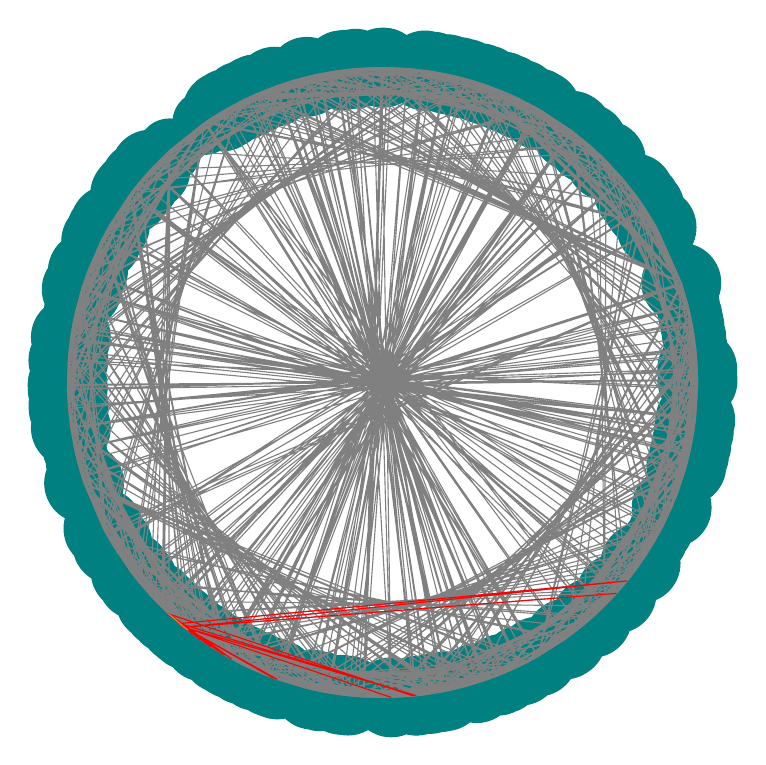
\begin{tikzpicture}
\filldraw[fill=teal, draw=teal]
(0.0,4.0) circle (0.5)(0.012271827051863905,3.9999811752383048) circle (0.5)(0.0613568251399524,3.9995293898168502) circle (0.4)(3.9995293898168502,-0.061356825139952394) circle (0.30000000000000004)(3.999077621404861,-0.08589632110187793) circle (0.4)(0.11043258311586296,3.9984752899807146) circle (0.4)(-0.24528294520883298,-3.9924724516005967) circle (0.4)(-3.990045824561214,0.282018293558456) circle (0.5)(0.3187297518857205,3.9872811971646627) circle (0.4)(-0.3187297518857198,-3.987281197164663) circle (0.4)(-3.9841788036050083,0.355414210330096) circle (0.4)(-0.37985398131855463,-3.9819230219677078) circle (0.4)(-3.9795173231792225,0.4042794510193105) circle (0.4)(-0.440888829175532,-3.9756278800094242) circle (0.5)(3.974256542082381,-0.45308380871025694) circle (0.4)(3.9714016578394604,-0.4774608592439649) circle (0.5)(-0.5261601148115324,-3.9652434393844618) circle (0.5)(0.5383228340285047,3.96361054171112) circle (0.5)(-3.961940337025828,0.5504804863459447) circle (0.4)(-3.9584880698528035,0.5747801326011773) circle (0.5)(3.953030270922998,-0.6111887410337732) circle (0.5)(3.9511365665782887,-0.6233135906170608) circle (0.5)(0.6354325733354458,3.9492056726314337) circle (0.5)(-3.945232388978395,0.6596524819598776) circle (0.4)(3.94319003667027,-0.6717531798989244) circle (0.4)(-0.6838475550412039,-3.9411105695557653) circle (0.4)(-0.7080168816485948,-3.9368403695477165) circle (0.4)(-3.934649676846921,0.7200916056227988) circle (0.4)(-3.9278554764382214,0.7562746565992224) circle (0.30000000000000004)(3.9207285438724697,-0.7923936428718145) circle (0.5)(-0.7923936428718142,-3.9207285438724697) circle (0.5)(0.8164358643712675,3.915792701276249) circle (0.5)(0.8284455047688742,3.9132694828785106) circle (0.5)(3.9028085201541143,-0.8764049606274786) circle (0.4)(-0.8883744838928137,-3.9001013802679765) circle (0.5)(3.8973575311423034,-0.9003356454391707) circle (0.4)(-3.894576998603248,0.912288332683543) circle (0.4)(3.8917598088222407,-0.9242324331226845) circle (0.5)(0.9719207196130555,3.880125012778176) circle (0.5)(-0.9957104229828795,-3.8740883770976695) circle (0.4)(3.858359173159251,-1.0550187158993256) circle (0.5)(1.0550187158993254,3.858359173159251) circle (0.5)(3.8417220776622636,-1.1140787575402118) circle (0.4)(3.8348138995834864,-1.1376301488450868) circle (0.4)(-3.8205646732230836,1.1846035529744932) circle (0.5)(1.196319305232162,3.8169123804364227) circle (0.4)(-3.813224161416775,1.2080237972769126) circle (0.4)(1.243068610998446,3.801944295797927) circle (0.5)(1.31283937431637,3.778419349045921) circle (0.5)(-1.3359986057680364,-3.770292790405788) circle (0.5)(-1.3706428692479768,-3.75783689440876) circle (0.5)(3.7536141362524327,-1.3821652998559562) circle (0.4)(-1.3936747209977383,-3.7493560476503) circle (0.5)(-3.745062668681114,1.4051710243422662) circle (0.5)(-3.740734039755791,1.4166541016819603) circle (0.5)(-1.4281238449337204,-3.7363702016170355) circle (0.5)(1.5307337294603591,3.695518130045147) circle (0.5)(3.671603102485562,-1.5872399496668412) circle (0.5)(-1.6097386034376733,-3.6617948643530713) circle (0.5)(1.6097386034376737,3.6617948643530713) circle (0.5)(1.654553248953738,3.641765169032269) circle (0.4)(-1.7213059253603307,-3.6106932729490353) circle (0.4)(-1.7544649541541093,-3.594697862775816) circle (0.4)(1.7544649541541106,3.5946978627758153) circle (0.5)(-1.7764885782817164,-3.583864999024741) circle (0.5)(-3.5728972047820613,1.7984453186184264) circle (0.5)(3.572897204782061,-1.7984453186184268) circle (0.4)(3.5448901205955226,-1.8530391342074406) circle (0.4)(3.52768505739342,-1.8855869473039908) circle (0.4)(-1.9179750306406123,-3.510181160829045) circle (0.5)(-3.5042803767816277,1.9287350883164889) circle (0.5)(-1.9502006405937427,-3.492379913673161) circle (0.5)(1.9609059331531646,3.486380346623804) circle (0.5)(1.9929106678911275,3.4681849820627706) circle (0.4)(3.4620544963622764,-2.0035415304449633) circle (0.4)(-2.003541530444963,-3.4620544963622764) circle (0.4)(-3.4620544963622764,2.003541530444963) circle (0.5)(2.0141535349028703,3.4558914244863472) circle (0.5)(-2.02474658138062,-3.449695824444163) circle (0.4)(-2.0353205701724284,-3.4434677545510692) circle (0.4)(-2.045875401751881,-3.437207273428034) circle (0.5)(3.392481379213189,-2.119214498745179) circle (0.30000000000000004)(-2.1812999536881845,-3.3528988222193528) circle (0.4)(3.346190908894048,-2.1915762366924008) circle (0.4)(-2.2120668223201094,-3.332680658807653) circle (0.4)(-2.273035810680526,-3.2913991255033057) circle (0.5)(3.2773900803071885,-2.293188666792168) circle (0.5)(-2.313255185646622,-3.2632576432269356) circle (0.30000000000000004)(3.2128301259225798,-2.3827972179697334) circle (0.4)(-3.2055046868925614,2.392642827985368) circle (0.5)(-2.4024659175354746,-3.198149076431621) circle (0.4)(2.402465917535476,3.19814907643162) circle (0.5)(2.422044165617302,3.1833476184355343) circle (0.5)(-3.1759019102173482,2.431799139871095) circle (0.5)(-2.470589231751215,-3.1458208543963435) circle (0.5)(-2.518552955659708,-3.1075538626929298) circle (0.4)(3.1075538626929298,-2.5185529556597084) circle (0.4)(-2.528074943759236,-3.0998124263794957) circle (0.5)(-3.076413350582319,2.5564977794551025) circle (0.5)(-2.575326171559165,-3.0606690624898363) circle (0.5)(2.6033867399855235,3.0368367559135523) circle (0.5)(3.0288353860259387,-2.612691371815106) circle (0.4)(2.9884024239207205,-2.6588439128133796) circle (0.4)(2.9720318085404873,-2.6771303533865436) circle (0.5)(-2.94726627550948,2.704370814301263) circle (0.5)(-2.713400172519445,-2.938955512383855) circle (0.5)(2.749261363567036,2.905436620337384) circle (0.4)(-2.775885843558615,-2.8800100318455275) circle (0.4)(-2.793504997635891,-2.862923301135275) circle (0.5)(-2.802275175772993,-2.854339475123175) circle (0.4)(2.8370913057554628,2.81973632150362) circle (0.5)(2.81973632150362,-2.837091305755462) circle (0.4)(-2.8800100318455266,-2.775885843558616) circle (0.5)(-2.704370814301264,2.947266275509479) circle (0.4)(-2.947266275509479,-2.704370814301264) circle (0.4)(2.686235819388074,-2.9638045014198355) circle (0.4)(2.65884391281338,-2.98840242392072) circle (0.5)(3.052753669053525,2.5847040519332656) circle (0.4)(-3.076413350582318,-2.556497779455104) circle (0.4)(2.518552955659709,-3.1075538626929293) circle (0.4)(-3.1152660495259026,-2.5090072619805777) circle (0.5)(-3.1759019102173474,-2.4317991398710963) circle (0.4)(3.19814907643162,2.402465917535476) circle (0.5)(-3.198149076431619,-2.4024659175354772) circle (0.5)(2.333234611750794,-3.249002346340815) circle (0.5)(2.313255185646623,-3.263257643226935) circle (0.5)(3.2773900803071876,2.2931886667921693) circle (0.5)(-2.2629272431344543,3.2983572111401003) circle (0.4)(-2.2426463047893463,3.3121801810310214) circle (0.4)(3.325878449210181,2.222280932078409) circle (0.5)(3.3326806588076527,2.2120668223201103) circle (0.4)(-2.139990479548389,3.379414260998828) circle (0.4)(-3.430914440001088,-2.056410976772887) circle (0.5)(-2.0353205701724297,3.4434677545510683) circle (0.5)(1.9715927689191366,-3.4803479644348454) circle (0.5)(3.4803479644348454,1.9715927689191364) circle (0.5)(-1.971592768919137,3.4803479644348454) circle (0.5)(-3.4983466091127045,-1.9394769920031647) circle (0.4)(-3.5160489057145337,-1.9071969202532886) circle (0.4)(-3.544890120595522,-1.8530391342074415) circle (0.5)(1.842154843832961,-3.5505584816114153) circle (0.4)(-1.798445318618428,3.5728972047820604) circle (0.5)(1.7544649541541102,-3.5946978627758157) circle (0.5)(1.7323752754126083,-3.6053953881840877) circle (0.4)(-1.732375275412609,3.6053953881840877) circle (0.4)(-1.6880010831991983,3.626382818059662) circle (0.4)(-1.6545532489537407,3.6417651690322677) circle (0.5)(-1.6097386034376748,3.661794864353071) circle (0.5)(-1.5872399496668432,3.671603102485561) circle (0.4)(1.5307337294603596,-3.695518130045147) circle (0.5)(1.4624519912190952,-3.723067844315935) circle (0.5)(-1.3706428692479797,3.757836894408759) circle (0.5)(-1.3591075376273085,3.7620242823730727) circle (0.4)(1.3128393743163709,-3.7784193490459206) circle (0.4)(1.2896307152042794,-3.786403652333134) circle (0.30000000000000004)(-3.790342364070965,-1.2780081232640617) circle (0.5)(1.2780081232640632,-3.7903423640709644) circle (0.4)(3.794245399662921,1.2663735022246634) circle (0.5)(-1.266373502224665,3.7942453996629206) circle (0.4)(3.801944295797927,1.243068610998446) circle (0.4)(1.1963193052321621,-3.8169123804364222) circle (0.5)(-3.8169123804364222,-1.1963193052321623) circle (0.4)(-1.1493898381789174,3.8313056521101316) circle (0.4)(-1.1022872772438337,3.845121943245282) circle (0.4)(1.090485421799797,-3.848485617076166) circle (0.4)(-1.0904854217997957,3.8484856170761663) circle (0.4)(-3.8710153483739016,-1.007591272616869) circle (0.4)(0.9957104229828804,-3.8740883770976695) circle (0.4)(3.877124941426194,0.9838202013431784) circle (0.4)(-0.9600120897949658,3.8830885629158014) circle (0.5)(-0.9122883326835447,3.8945769986032475) circle (0.30000000000000004)(3.9054789253200846,0.8644271883048784) circle (0.4)(0.8524412796643657,-3.908112570631017) circle (0.4)(-3.908112570631017,-0.8524412796643677) circle (0.4)(-0.8164358643712696,3.9157927012762483) circle (0.4)(0.7923936428718152,-3.9207285438724693) circle (0.5)(-0.7923936428718139,3.9207285438724697) circle (0.4)(0.7683215881995699,-3.9255167732550182) circle (0.4)(3.9255167732550182,0.7683215881995696) circle (0.4)(0.7442206066537876,-3.930157209149765) circle (0.5)(3.934649676846921,0.7200916056227981) circle (0.4)(0.6111887410337747,-3.953030270922998) circle (0.4)(0.5990581387092858,-3.954886767841295) circle (0.5)(-0.5990581387092864,3.954886767841295) circle (0.4)(3.956706039859124,0.586921897821447) circle (0.4)(-3.958488069852803,-0.5747801326011788) circle (0.5)(0.5383228340285051,-3.96361054171112) circle (0.4)(-0.5139924431751746,3.9668390146763977) circle (0.5)(-0.46527452364761934,3.972847796939178) circle (0.5)(3.9756278800094242,0.44088882917553274) circle (0.4)(0.42868969982723665,-3.9769617978127516) circle (0.5)(3.9795173231792225,0.4042794510193115) circle (0.30000000000000004)(0.3920685613182433,-3.9807389066887873) circle (0.4)(3.984178803605008,0.35541421033009873) circle (0.4)(-0.34318924937776113,3.985250448731112) circle (0.5)(-3.9862845831622193,-0.3309610581975028) circle (0.5)(3.9862845831622193,0.3309610581975032) circle (0.4)(-3.989161826714761,-0.2942582543986694) circle (0.5)(3.9963109110105814,0.17175302773976384) circle (0.5)(3.997722418221847,0.13496468740551057) circle (0.5)(-0.12269921270654617,3.9981176700043726) circle (0.4)(0.11043258311586264,-3.9984752899807146) circle (0.5)(-3.999077621404861,-0.08589632110187714) circle (0.5)(-3.9998305782078556,-0.03681501912824033) circle (0.5)(3.9998305782078556,0.03681501912823984) circle (0.5)(3.9999247011304044,0.02454353859661806) circle (0.5)(-3.9999247011304044,-0.024543538596617665) circle (0.5)(-0.012271827051866175,3.9999811752383048) circle (0.4);
\draw [gray]
(0.0,4.0) -- (0.012271827051863905,3.9999811752383048)
(0.0,4.0) -- (0.0613568251399524,3.9995293898168502)
(0.0,4.0) -- (0.0613568251399524,3.9995293898168502)
(0.0,4.0) -- (0.11043258311586296,3.9984752899807146)
(0.0,4.0) -- (0.3187297518857205,3.9872811971646627)
(0.0,4.0) -- (0.5383228340285047,3.96361054171112)
(0.0,4.0) -- (0.8164358643712675,3.915792701276249)
(0.0,4.0) -- (1.5307337294603591,3.695518130045147)
(0.0,4.0) -- (2.8370913057554628,2.81973632150362)
(0.0,4.0) -- (3.9995293898168502,-0.061356825139952394)
(0.0,4.0) -- (-0.24528294520883298,-3.9924724516005967)
(0.012271827051863905,3.9999811752383048) -- (0.0613568251399524,3.9995293898168502)
(0.012271827051863905,3.9999811752383048) -- (0.0613568251399524,3.9995293898168502)
(0.012271827051863905,3.9999811752383048) -- (0.0613568251399524,3.9995293898168502)
(0.012271827051863905,3.9999811752383048) -- (0.11043258311586296,3.9984752899807146)
(0.012271827051863905,3.9999811752383048) -- (0.3187297518857205,3.9872811971646627)
(0.012271827051863905,3.9999811752383048) -- (0.5383228340285047,3.96361054171112)
(0.012271827051863905,3.9999811752383048) -- (0.8164358643712675,3.915792701276249)
(0.012271827051863905,3.9999811752383048) -- (1.6097386034376737,3.6617948643530713)
(0.012271827051863905,3.9999811752383048) -- (2.8370913057554628,2.81973632150362)
(0.012271827051863905,3.9999811752383048) -- (3.9995293898168502,-0.061356825139952394)
(0.012271827051863905,3.9999811752383048) -- (-0.24528294520883298,-3.9924724516005967)
(0.0613568251399524,3.9995293898168502) -- (0.11043258311586296,3.9984752899807146)
(0.0613568251399524,3.9995293898168502) -- (0.11043258311586296,3.9984752899807146)
(0.0613568251399524,3.9995293898168502) -- (0.11043258311586296,3.9984752899807146)
(0.0613568251399524,3.9995293898168502) -- (0.3187297518857205,3.9872811971646627)
(0.0613568251399524,3.9995293898168502) -- (0.3187297518857205,3.9872811971646627)
(0.0613568251399524,3.9995293898168502) -- (0.5383228340285047,3.96361054171112)
(0.0613568251399524,3.9995293898168502) -- (0.9719207196130555,3.880125012778176)
(0.0613568251399524,3.9995293898168502) -- (1.6097386034376737,3.6617948643530713)
(0.0613568251399524,3.9995293898168502) -- (3.052753669053525,2.5847040519332656)
(0.0613568251399524,3.9995293898168502) -- (3.9995293898168502,-0.061356825139952394)
(0.0613568251399524,3.9995293898168502) -- (-0.24528294520883298,-3.9924724516005967)
(3.9995293898168502,-0.061356825139952394) -- (3.999077621404861,-0.08589632110187793)
(3.9995293898168502,-0.061356825139952394) -- (3.999077621404861,-0.08589632110187793)
(3.9995293898168502,-0.061356825139952394) -- (3.974256542082381,-0.45308380871025694)
(3.9995293898168502,-0.061356825139952394) -- (3.974256542082381,-0.45308380871025694)
(3.9995293898168502,-0.061356825139952394) -- (3.974256542082381,-0.45308380871025694)
(3.9995293898168502,-0.061356825139952394) -- (3.974256542082381,-0.45308380871025694)
(3.9995293898168502,-0.061356825139952394) -- (3.9028085201541143,-0.8764049606274786)
(3.9995293898168502,-0.061356825139952394) -- (3.671603102485562,-1.5872399496668412)
(3.9995293898168502,-0.061356825139952394) -- (2.686235819388074,-2.9638045014198355)
(3.9995293898168502,-0.061356825139952394) -- (-0.24528294520883298,-3.9924724516005967)
(3.9995293898168502,-0.061356825139952394) -- (-3.990045824561214,0.282018293558456)
(3.999077621404861,-0.08589632110187793) -- (3.974256542082381,-0.45308380871025694)
(3.999077621404861,-0.08589632110187793) -- (3.974256542082381,-0.45308380871025694)
(3.999077621404861,-0.08589632110187793) -- (3.974256542082381,-0.45308380871025694)
(3.999077621404861,-0.08589632110187793) -- (3.974256542082381,-0.45308380871025694)
(3.999077621404861,-0.08589632110187793) -- (3.974256542082381,-0.45308380871025694)
(3.999077621404861,-0.08589632110187793) -- (3.9714016578394604,-0.4774608592439649)
(3.999077621404861,-0.08589632110187793) -- (3.9028085201541143,-0.8764049606274786)
(3.999077621404861,-0.08589632110187793) -- (3.572897204782061,-1.7984453186184268)
(3.999077621404861,-0.08589632110187793) -- (2.686235819388074,-2.9638045014198355)
(3.999077621404861,-0.08589632110187793) -- (-0.24528294520883298,-3.9924724516005967)
(3.999077621404861,-0.08589632110187793) -- (-3.990045824561214,0.282018293558456)
(0.11043258311586296,3.9984752899807146) -- (0.3187297518857205,3.9872811971646627)
(0.11043258311586296,3.9984752899807146) -- (0.3187297518857205,3.9872811971646627)
(0.11043258311586296,3.9984752899807146) -- (0.3187297518857205,3.9872811971646627)
(0.11043258311586296,3.9984752899807146) -- (0.3187297518857205,3.9872811971646627)
(0.11043258311586296,3.9984752899807146) -- (0.3187297518857205,3.9872811971646627)
(0.11043258311586296,3.9984752899807146) -- (0.5383228340285047,3.96361054171112)
(0.11043258311586296,3.9984752899807146) -- (0.9719207196130555,3.880125012778176)
(0.11043258311586296,3.9984752899807146) -- (1.654553248953738,3.641765169032269)
(0.11043258311586296,3.9984752899807146) -- (3.052753669053525,2.5847040519332656)
(0.11043258311586296,3.9984752899807146) -- (3.974256542082381,-0.45308380871025694)
(0.11043258311586296,3.9984752899807146) -- (-0.24528294520883298,-3.9924724516005967)
(-0.24528294520883298,-3.9924724516005967) -- (-0.3187297518857198,-3.987281197164663)
(-0.24528294520883298,-3.9924724516005967) -- (-0.3187297518857198,-3.987281197164663)
(-0.24528294520883298,-3.9924724516005967) -- (-0.3187297518857198,-3.987281197164663)
(-0.24528294520883298,-3.9924724516005967) -- (-0.37985398131855463,-3.9819230219677078)
(-0.24528294520883298,-3.9924724516005967) -- (-0.440888829175532,-3.9756278800094242)
(-0.24528294520883298,-3.9924724516005967) -- (-0.6838475550412039,-3.9411105695557653)
(-0.24528294520883298,-3.9924724516005967) -- (-1.3359986057680364,-3.770292790405788)
(-0.24528294520883298,-3.9924724516005967) -- (-1.7544649541541093,-3.594697862775816)
(-0.24528294520883298,-3.9924724516005967) -- (-3.076413350582318,-2.556497779455104)
(-0.24528294520883298,-3.9924724516005967) -- (-3.990045824561214,0.282018293558456)
(-0.24528294520883298,-3.9924724516005967) -- (0.3187297518857205,3.9872811971646627)
(-3.990045824561214,0.282018293558456) -- (-3.9841788036050083,0.355414210330096)
(-3.990045824561214,0.282018293558456) -- (-3.9841788036050083,0.355414210330096)
(-3.990045824561214,0.282018293558456) -- (-3.9841788036050083,0.355414210330096)
(-3.990045824561214,0.282018293558456) -- (-3.9795173231792225,0.4042794510193105)
(-3.990045824561214,0.282018293558456) -- (-3.961940337025828,0.5504804863459447)
(-3.990045824561214,0.282018293558456) -- (-3.934649676846921,0.7200916056227988)
(-3.990045824561214,0.282018293558456) -- (-3.8205646732230836,1.1846035529744932)
(-3.990045824561214,0.282018293558456) -- (-3.5728972047820613,1.7984453186184264)
(-3.990045824561214,0.282018293558456) -- (-2.2629272431344543,3.2983572111401003)
(-3.990045824561214,0.282018293558456) -- (0.3187297518857205,3.9872811971646627)
(-3.990045824561214,0.282018293558456) -- (3.974256542082381,-0.45308380871025694)
(0.3187297518857205,3.9872811971646627) -- (0.5383228340285047,3.96361054171112)
(0.3187297518857205,3.9872811971646627) -- (0.5383228340285047,3.96361054171112)
(0.3187297518857205,3.9872811971646627) -- (0.5383228340285047,3.96361054171112)
(0.3187297518857205,3.9872811971646627) -- (0.5383228340285047,3.96361054171112)
(0.3187297518857205,3.9872811971646627) -- (0.5383228340285047,3.96361054171112)
(0.3187297518857205,3.9872811971646627) -- (0.8164358643712675,3.915792701276249)
(0.3187297518857205,3.9872811971646627) -- (1.196319305232162,3.8169123804364227)
(0.3187297518857205,3.9872811971646627) -- (1.9609059331531646,3.486380346623804)
(0.3187297518857205,3.9872811971646627) -- (3.052753669053525,2.5847040519332656)
(0.3187297518857205,3.9872811971646627) -- (3.974256542082381,-0.45308380871025694)
(0.3187297518857205,3.9872811971646627) -- (-0.3187297518857198,-3.987281197164663)
(-0.3187297518857198,-3.987281197164663) -- (-0.37985398131855463,-3.9819230219677078)
(-0.3187297518857198,-3.987281197164663) -- (-0.37985398131855463,-3.9819230219677078)
(-0.3187297518857198,-3.987281197164663) -- (-0.37985398131855463,-3.9819230219677078)
(-0.3187297518857198,-3.987281197164663) -- (-0.440888829175532,-3.9756278800094242)
(-0.3187297518857198,-3.987281197164663) -- (-0.5261601148115324,-3.9652434393844618)
(-0.3187297518857198,-3.987281197164663) -- (-0.7080168816485948,-3.9368403695477165)
(-0.3187297518857198,-3.987281197164663) -- (-1.3359986057680364,-3.770292790405788)
(-0.3187297518857198,-3.987281197164663) -- (-1.9179750306406123,-3.510181160829045)
(-0.3187297518857198,-3.987281197164663) -- (-3.076413350582318,-2.556497779455104)
(-0.3187297518857198,-3.987281197164663) -- (-3.9841788036050083,0.355414210330096)
(-0.3187297518857198,-3.987281197164663) -- (0.3187297518857205,3.9872811971646627)
(-3.9841788036050083,0.355414210330096) -- (-3.9795173231792225,0.4042794510193105)
(-3.9841788036050083,0.355414210330096) -- (-3.9795173231792225,0.4042794510193105)
(-3.9841788036050083,0.355414210330096) -- (-3.9795173231792225,0.4042794510193105)
(-3.9841788036050083,0.355414210330096) -- (-3.961940337025828,0.5504804863459447)
(-3.9841788036050083,0.355414210330096) -- (-3.961940337025828,0.5504804863459447)
(-3.9841788036050083,0.355414210330096) -- (-3.9278554764382214,0.7562746565992224)
(-3.9841788036050083,0.355414210330096) -- (-3.8205646732230836,1.1846035529744932)
(-3.9841788036050083,0.355414210330096) -- (-3.5042803767816277,1.9287350883164889)
(-3.9841788036050083,0.355414210330096) -- (-2.2629272431344543,3.2983572111401003)
(-3.9841788036050083,0.355414210330096) -- (0.5383228340285047,3.96361054171112)
(-3.9841788036050083,0.355414210330096) -- (3.974256542082381,-0.45308380871025694)
(-0.37985398131855463,-3.9819230219677078) -- (-0.440888829175532,-3.9756278800094242)
(-0.37985398131855463,-3.9819230219677078) -- (-0.440888829175532,-3.9756278800094242)
(-0.37985398131855463,-3.9819230219677078) -- (-0.440888829175532,-3.9756278800094242)
(-0.37985398131855463,-3.9819230219677078) -- (-0.5261601148115324,-3.9652434393844618)
(-0.37985398131855463,-3.9819230219677078) -- (-0.6838475550412039,-3.9411105695557653)
(-0.37985398131855463,-3.9819230219677078) -- (-0.7923936428718142,-3.9207285438724697)
(-0.37985398131855463,-3.9819230219677078) -- (-1.3359986057680364,-3.770292790405788)
(-0.37985398131855463,-3.9819230219677078) -- (-1.9179750306406123,-3.510181160829045)
(-0.37985398131855463,-3.9819230219677078) -- (-3.1152660495259026,-2.5090072619805777)
(-0.37985398131855463,-3.9819230219677078) -- (-3.9795173231792225,0.4042794510193105)
(-0.37985398131855463,-3.9819230219677078) -- (0.5383228340285047,3.96361054171112)
(-3.9795173231792225,0.4042794510193105) -- (-3.961940337025828,0.5504804863459447)
(-3.9795173231792225,0.4042794510193105) -- (-3.961940337025828,0.5504804863459447)
(-3.9795173231792225,0.4042794510193105) -- (-3.961940337025828,0.5504804863459447)
(-3.9795173231792225,0.4042794510193105) -- (-3.961940337025828,0.5504804863459447)
(-3.9795173231792225,0.4042794510193105) -- (-3.945232388978395,0.6596524819598776)
(-3.9795173231792225,0.4042794510193105) -- (-3.894576998603248,0.912288332683543)
(-3.9795173231792225,0.4042794510193105) -- (-3.8205646732230836,1.1846035529744932)
(-3.9795173231792225,0.4042794510193105) -- (-3.5042803767816277,1.9287350883164889)
(-3.9795173231792225,0.4042794510193105) -- (-2.2629272431344543,3.2983572111401003)
(-3.9795173231792225,0.4042794510193105) -- (0.5383228340285047,3.96361054171112)
(-3.9795173231792225,0.4042794510193105) -- (3.974256542082381,-0.45308380871025694)
(-0.440888829175532,-3.9756278800094242) -- (-0.5261601148115324,-3.9652434393844618)
(-0.440888829175532,-3.9756278800094242) -- (-0.5261601148115324,-3.9652434393844618)
(-0.440888829175532,-3.9756278800094242) -- (-0.5261601148115324,-3.9652434393844618)
(-0.440888829175532,-3.9756278800094242) -- (-0.6838475550412039,-3.9411105695557653)
(-0.440888829175532,-3.9756278800094242) -- (-0.6838475550412039,-3.9411105695557653)
(-0.440888829175532,-3.9756278800094242) -- (-0.8883744838928137,-3.9001013802679765)
(-0.440888829175532,-3.9756278800094242) -- (-1.3359986057680364,-3.770292790405788)
(-0.440888829175532,-3.9756278800094242) -- (-1.9502006405937427,-3.492379913673161)
(-0.440888829175532,-3.9756278800094242) -- (-3.1759019102173474,-2.4317991398710963)
(-0.440888829175532,-3.9756278800094242) -- (-3.961940337025828,0.5504804863459447)
(-0.440888829175532,-3.9756278800094242) -- (0.5383228340285047,3.96361054171112)
(3.974256542082381,-0.45308380871025694) -- (3.9714016578394604,-0.4774608592439649)
(3.974256542082381,-0.45308380871025694) -- (3.9714016578394604,-0.4774608592439649)
(3.974256542082381,-0.45308380871025694) -- (3.953030270922998,-0.6111887410337732)
(3.974256542082381,-0.45308380871025694) -- (3.953030270922998,-0.6111887410337732)
(3.974256542082381,-0.45308380871025694) -- (3.94319003667027,-0.6717531798989244)
(3.974256542082381,-0.45308380871025694) -- (3.9028085201541143,-0.8764049606274786)
(3.974256542082381,-0.45308380871025694) -- (3.7536141362524327,-1.3821652998559562)
(3.974256542082381,-0.45308380871025694) -- (3.4620544963622764,-2.0035415304449633)
(3.974256542082381,-0.45308380871025694) -- (2.333234611750794,-3.249002346340815)
(3.974256542082381,-0.45308380871025694) -- (-0.5261601148115324,-3.9652434393844618)
(3.974256542082381,-0.45308380871025694) -- (-3.961940337025828,0.5504804863459447)
(3.9714016578394604,-0.4774608592439649) -- (3.953030270922998,-0.6111887410337732)
(3.9714016578394604,-0.4774608592439649) -- (3.953030270922998,-0.6111887410337732)
(3.9714016578394604,-0.4774608592439649) -- (3.953030270922998,-0.6111887410337732)
(3.9714016578394604,-0.4774608592439649) -- (3.953030270922998,-0.6111887410337732)
(3.9714016578394604,-0.4774608592439649) -- (3.94319003667027,-0.6717531798989244)
(3.9714016578394604,-0.4774608592439649) -- (3.9028085201541143,-0.8764049606274786)
(3.9714016578394604,-0.4774608592439649) -- (3.7536141362524327,-1.3821652998559562)
(3.9714016578394604,-0.4774608592439649) -- (3.4620544963622764,-2.0035415304449633)
(3.9714016578394604,-0.4774608592439649) -- (2.333234611750794,-3.249002346340815)
(3.9714016578394604,-0.4774608592439649) -- (-0.5261601148115324,-3.9652434393844618)
(3.9714016578394604,-0.4774608592439649) -- (-3.961940337025828,0.5504804863459447)
(-0.5261601148115324,-3.9652434393844618) -- (-0.6838475550412039,-3.9411105695557653)
(-0.5261601148115324,-3.9652434393844618) -- (-0.6838475550412039,-3.9411105695557653)
(-0.5261601148115324,-3.9652434393844618) -- (-0.6838475550412039,-3.9411105695557653)
(-0.5261601148115324,-3.9652434393844618) -- (-0.6838475550412039,-3.9411105695557653)
(-0.5261601148115324,-3.9652434393844618) -- (-0.7923936428718142,-3.9207285438724697)
(-0.5261601148115324,-3.9652434393844618) -- (-0.9957104229828795,-3.8740883770976695)
(-0.5261601148115324,-3.9652434393844618) -- (-1.3359986057680364,-3.770292790405788)
(-0.5261601148115324,-3.9652434393844618) -- (-2.003541530444963,-3.4620544963622764)
(-0.5261601148115324,-3.9652434393844618) -- (-3.1759019102173474,-2.4317991398710963)
(-0.5261601148115324,-3.9652434393844618) -- (-3.961940337025828,0.5504804863459447)
(-0.5261601148115324,-3.9652434393844618) -- (0.5383228340285047,3.96361054171112)
(0.5383228340285047,3.96361054171112) -- (0.6354325733354458,3.9492056726314337)
(0.5383228340285047,3.96361054171112) -- (0.6354325733354458,3.9492056726314337)
(0.5383228340285047,3.96361054171112) -- (0.6354325733354458,3.9492056726314337)
(0.5383228340285047,3.96361054171112) -- (0.6354325733354458,3.9492056726314337)
(0.5383228340285047,3.96361054171112) -- (0.8164358643712675,3.915792701276249)
(0.5383228340285047,3.96361054171112) -- (0.9719207196130555,3.880125012778176)
(0.5383228340285047,3.96361054171112) -- (1.31283937431637,3.778419349045921)
(0.5383228340285047,3.96361054171112) -- (2.0141535349028703,3.4558914244863472)
(0.5383228340285047,3.96361054171112) -- (3.19814907643162,2.402465917535476)
(0.5383228340285047,3.96361054171112) -- (3.953030270922998,-0.6111887410337732)
(0.5383228340285047,3.96361054171112) -- (-0.6838475550412039,-3.9411105695557653)
(-3.961940337025828,0.5504804863459447) -- (-3.9584880698528035,0.5747801326011773)
(-3.961940337025828,0.5504804863459447) -- (-3.9584880698528035,0.5747801326011773)
(-3.961940337025828,0.5504804863459447) -- (-3.945232388978395,0.6596524819598776)
(-3.961940337025828,0.5504804863459447) -- (-3.945232388978395,0.6596524819598776)
(-3.961940337025828,0.5504804863459447) -- (-3.9278554764382214,0.7562746565992224)
(-3.961940337025828,0.5504804863459447) -- (-3.8205646732230836,1.1846035529744932)
(-3.961940337025828,0.5504804863459447) -- (-3.745062668681114,1.4051710243422662)
(-3.961940337025828,0.5504804863459447) -- (-3.2055046868925614,2.392642827985368)
(-3.961940337025828,0.5504804863459447) -- (-2.2629272431344543,3.2983572111401003)
(-3.961940337025828,0.5504804863459447) -- (0.6354325733354458,3.9492056726314337)
(-3.961940337025828,0.5504804863459447) -- (3.953030270922998,-0.6111887410337732)
(-3.9584880698528035,0.5747801326011773) -- (-3.945232388978395,0.6596524819598776)
(-3.9584880698528035,0.5747801326011773) -- (-3.945232388978395,0.6596524819598776)
(-3.9584880698528035,0.5747801326011773) -- (-3.945232388978395,0.6596524819598776)
(-3.9584880698528035,0.5747801326011773) -- (-3.934649676846921,0.7200916056227988)
(-3.9584880698528035,0.5747801326011773) -- (-3.894576998603248,0.912288332683543)
(-3.9584880698528035,0.5747801326011773) -- (-3.8205646732230836,1.1846035529744932)
(-3.9584880698528035,0.5747801326011773) -- (-3.745062668681114,1.4051710243422662)
(-3.9584880698528035,0.5747801326011773) -- (-3.2055046868925614,2.392642827985368)
(-3.9584880698528035,0.5747801326011773) -- (-2.2629272431344543,3.2983572111401003)
(-3.9584880698528035,0.5747801326011773) -- (0.6354325733354458,3.9492056726314337)
(-3.9584880698528035,0.5747801326011773) -- (3.953030270922998,-0.6111887410337732)
(3.953030270922998,-0.6111887410337732) -- (3.9511365665782887,-0.6233135906170608)
(3.953030270922998,-0.6111887410337732) -- (3.94319003667027,-0.6717531798989244)
(3.953030270922998,-0.6111887410337732) -- (3.94319003667027,-0.6717531798989244)
(3.953030270922998,-0.6111887410337732) -- (3.9207285438724697,-0.7923936428718145)
(3.953030270922998,-0.6111887410337732) -- (3.9028085201541143,-0.8764049606274786)
(3.953030270922998,-0.6111887410337732) -- (3.858359173159251,-1.0550187158993256)
(3.953030270922998,-0.6111887410337732) -- (3.7536141362524327,-1.3821652998559562)
(3.953030270922998,-0.6111887410337732) -- (3.392481379213189,-2.119214498745179)
(3.953030270922998,-0.6111887410337732) -- (2.333234611750794,-3.249002346340815)
(3.953030270922998,-0.6111887410337732) -- (-0.6838475550412039,-3.9411105695557653)
(3.953030270922998,-0.6111887410337732) -- (-3.945232388978395,0.6596524819598776)
(3.9511365665782887,-0.6233135906170608) -- (3.94319003667027,-0.6717531798989244)
(3.9511365665782887,-0.6233135906170608) -- (3.94319003667027,-0.6717531798989244)
(3.9511365665782887,-0.6233135906170608) -- (3.94319003667027,-0.6717531798989244)
(3.9511365665782887,-0.6233135906170608) -- (3.9207285438724697,-0.7923936428718145)
(3.9511365665782887,-0.6233135906170608) -- (3.9028085201541143,-0.8764049606274786)
(3.9511365665782887,-0.6233135906170608) -- (3.858359173159251,-1.0550187158993256)
(3.9511365665782887,-0.6233135906170608) -- (3.7536141362524327,-1.3821652998559562)
(3.9511365665782887,-0.6233135906170608) -- (3.392481379213189,-2.119214498745179)
(3.9511365665782887,-0.6233135906170608) -- (2.333234611750794,-3.249002346340815)
(3.9511365665782887,-0.6233135906170608) -- (-0.6838475550412039,-3.9411105695557653)
(3.9511365665782887,-0.6233135906170608) -- (-3.945232388978395,0.6596524819598776)
(0.6354325733354458,3.9492056726314337) -- (0.8164358643712675,3.915792701276249)
(0.6354325733354458,3.9492056726314337) -- (0.8164358643712675,3.915792701276249)
(0.6354325733354458,3.9492056726314337) -- (0.8164358643712675,3.915792701276249)
(0.6354325733354458,3.9492056726314337) -- (0.8164358643712675,3.915792701276249)
(0.6354325733354458,3.9492056726314337) -- (0.8284455047688742,3.9132694828785106)
(0.6354325733354458,3.9492056726314337) -- (1.0550187158993254,3.858359173159251)
(0.6354325733354458,3.9492056726314337) -- (1.5307337294603591,3.695518130045147)
(0.6354325733354458,3.9492056726314337) -- (2.402465917535476,3.19814907643162)
(0.6354325733354458,3.9492056726314337) -- (3.2773900803071876,2.2931886667921693)
(0.6354325733354458,3.9492056726314337) -- (3.94319003667027,-0.6717531798989244)
(0.6354325733354458,3.9492056726314337) -- (-0.6838475550412039,-3.9411105695557653)
(-3.945232388978395,0.6596524819598776) -- (-3.934649676846921,0.7200916056227988)
(-3.945232388978395,0.6596524819598776) -- (-3.934649676846921,0.7200916056227988)
(-3.945232388978395,0.6596524819598776) -- (-3.934649676846921,0.7200916056227988)
(-3.945232388978395,0.6596524819598776) -- (-3.9278554764382214,0.7562746565992224)
(-3.945232388978395,0.6596524819598776) -- (-3.894576998603248,0.912288332683543)
(-3.945232388978395,0.6596524819598776) -- (-3.8205646732230836,1.1846035529744932)
(-3.945232388978395,0.6596524819598776) -- (-3.740734039755791,1.4166541016819603)
(-3.945232388978395,0.6596524819598776) -- (-3.2055046868925614,2.392642827985368)
(-3.945232388978395,0.6596524819598776) -- (-2.2629272431344543,3.2983572111401003)
(-3.945232388978395,0.6596524819598776) -- (0.8164358643712675,3.915792701276249)
(-3.945232388978395,0.6596524819598776) -- (3.94319003667027,-0.6717531798989244)
(3.94319003667027,-0.6717531798989244) -- (3.9207285438724697,-0.7923936428718145)
(3.94319003667027,-0.6717531798989244) -- (3.9207285438724697,-0.7923936428718145)
(3.94319003667027,-0.6717531798989244) -- (3.9207285438724697,-0.7923936428718145)
(3.94319003667027,-0.6717531798989244) -- (3.9207285438724697,-0.7923936428718145)
(3.94319003667027,-0.6717531798989244) -- (3.9028085201541143,-0.8764049606274786)
(3.94319003667027,-0.6717531798989244) -- (3.858359173159251,-1.0550187158993256)
(3.94319003667027,-0.6717531798989244) -- (3.671603102485562,-1.5872399496668412)
(3.94319003667027,-0.6717531798989244) -- (3.346190908894048,-2.1915762366924008)
(3.94319003667027,-0.6717531798989244) -- (2.313255185646623,-3.263257643226935)
(3.94319003667027,-0.6717531798989244) -- (-0.6838475550412039,-3.9411105695557653)
(3.94319003667027,-0.6717531798989244) -- (-3.934649676846921,0.7200916056227988)
(-0.6838475550412039,-3.9411105695557653) -- (-0.7080168816485948,-3.9368403695477165)
(-0.6838475550412039,-3.9411105695557653) -- (-0.7080168816485948,-3.9368403695477165)
(-0.6838475550412039,-3.9411105695557653) -- (-0.7923936428718142,-3.9207285438724697)
(-0.6838475550412039,-3.9411105695557653) -- (-0.7923936428718142,-3.9207285438724697)
(-0.6838475550412039,-3.9411105695557653) -- (-0.8883744838928137,-3.9001013802679765)
(-0.6838475550412039,-3.9411105695557653) -- (-1.3359986057680364,-3.770292790405788)
(-0.6838475550412039,-3.9411105695557653) -- (-1.6097386034376733,-3.6617948643530713)
(-0.6838475550412039,-3.9411105695557653) -- (-2.1812999536881845,-3.3528988222193528)
(-0.6838475550412039,-3.9411105695557653) -- (-3.430914440001088,-2.056410976772887)
(-0.6838475550412039,-3.9411105695557653) -- (-3.934649676846921,0.7200916056227988)
(-0.6838475550412039,-3.9411105695557653) -- (0.8164358643712675,3.915792701276249)
(-0.7080168816485948,-3.9368403695477165) -- (-0.7923936428718142,-3.9207285438724697)
(-0.7080168816485948,-3.9368403695477165) -- (-0.7923936428718142,-3.9207285438724697)
(-0.7080168816485948,-3.9368403695477165) -- (-0.7923936428718142,-3.9207285438724697)
(-0.7080168816485948,-3.9368403695477165) -- (-0.8883744838928137,-3.9001013802679765)
(-0.7080168816485948,-3.9368403695477165) -- (-0.9957104229828795,-3.8740883770976695)
(-0.7080168816485948,-3.9368403695477165) -- (-1.3359986057680364,-3.770292790405788)
(-0.7080168816485948,-3.9368403695477165) -- (-1.6097386034376733,-3.6617948643530713)
(-0.7080168816485948,-3.9368403695477165) -- (-2.1812999536881845,-3.3528988222193528)
(-0.7080168816485948,-3.9368403695477165) -- (-3.430914440001088,-2.056410976772887)
(-0.7080168816485948,-3.9368403695477165) -- (-3.934649676846921,0.7200916056227988)
(-0.7080168816485948,-3.9368403695477165) -- (0.8164358643712675,3.915792701276249)
(-3.934649676846921,0.7200916056227988) -- (-3.9278554764382214,0.7562746565992224)
(-3.934649676846921,0.7200916056227988) -- (-3.9278554764382214,0.7562746565992224)
(-3.934649676846921,0.7200916056227988) -- (-3.894576998603248,0.912288332683543)
(-3.934649676846921,0.7200916056227988) -- (-3.894576998603248,0.912288332683543)
(-3.934649676846921,0.7200916056227988) -- (-3.894576998603248,0.912288332683543)
(-3.934649676846921,0.7200916056227988) -- (-3.8205646732230836,1.1846035529744932)
(-3.934649676846921,0.7200916056227988) -- (-3.5728972047820613,1.7984453186184264)
(-3.934649676846921,0.7200916056227988) -- (-3.2055046868925614,2.392642827985368)
(-3.934649676846921,0.7200916056227988) -- (-2.2629272431344543,3.2983572111401003)
(-3.934649676846921,0.7200916056227988) -- (0.8164358643712675,3.915792701276249)
(-3.934649676846921,0.7200916056227988) -- (3.9207285438724697,-0.7923936428718145)
(-3.9278554764382214,0.7562746565992224) -- (-3.894576998603248,0.912288332683543)
(-3.9278554764382214,0.7562746565992224) -- (-3.894576998603248,0.912288332683543)
(-3.9278554764382214,0.7562746565992224) -- (-3.894576998603248,0.912288332683543)
(-3.9278554764382214,0.7562746565992224) -- (-3.894576998603248,0.912288332683543)
(-3.9278554764382214,0.7562746565992224) -- (-3.8205646732230836,1.1846035529744932)
(-3.9278554764382214,0.7562746565992224) -- (-3.8205646732230836,1.1846035529744932)
(-3.9278554764382214,0.7562746565992224) -- (-3.5728972047820613,1.7984453186184264)
(-3.9278554764382214,0.7562746565992224) -- (-3.2055046868925614,2.392642827985368)
(-3.9278554764382214,0.7562746565992224) -- (-2.2426463047893463,3.3121801810310214)
(-3.9278554764382214,0.7562746565992224) -- (0.8164358643712675,3.915792701276249)
(-3.9278554764382214,0.7562746565992224) -- (3.9207285438724697,-0.7923936428718145)
(3.9207285438724697,-0.7923936428718145) -- (3.9028085201541143,-0.8764049606274786)
(3.9207285438724697,-0.7923936428718145) -- (3.9028085201541143,-0.8764049606274786)
(3.9207285438724697,-0.7923936428718145) -- (3.9028085201541143,-0.8764049606274786)
(3.9207285438724697,-0.7923936428718145) -- (3.8973575311423034,-0.9003356454391707)
(3.9207285438724697,-0.7923936428718145) -- (3.858359173159251,-1.0550187158993256)
(3.9207285438724697,-0.7923936428718145) -- (3.7536141362524327,-1.3821652998559562)
(3.9207285438724697,-0.7923936428718145) -- (3.671603102485562,-1.5872399496668412)
(3.9207285438724697,-0.7923936428718145) -- (3.2773900803071885,-2.293188666792168)
(3.9207285438724697,-0.7923936428718145) -- (1.9715927689191366,-3.4803479644348454)
(3.9207285438724697,-0.7923936428718145) -- (-0.7923936428718142,-3.9207285438724697)
(3.9207285438724697,-0.7923936428718145) -- (-3.894576998603248,0.912288332683543)
(-0.7923936428718142,-3.9207285438724697) -- (-0.8883744838928137,-3.9001013802679765)
(-0.7923936428718142,-3.9207285438724697) -- (-0.8883744838928137,-3.9001013802679765)
(-0.7923936428718142,-3.9207285438724697) -- (-0.8883744838928137,-3.9001013802679765)
(-0.7923936428718142,-3.9207285438724697) -- (-0.8883744838928137,-3.9001013802679765)
(-0.7923936428718142,-3.9207285438724697) -- (-0.9957104229828795,-3.8740883770976695)
(-0.7923936428718142,-3.9207285438724697) -- (-1.3359986057680364,-3.770292790405788)
(-0.7923936428718142,-3.9207285438724697) -- (-1.6097386034376733,-3.6617948643530713)
(-0.7923936428718142,-3.9207285438724697) -- (-2.273035810680526,-3.2913991255033057)
(-0.7923936428718142,-3.9207285438724697) -- (-3.430914440001088,-2.056410976772887)
(-0.7923936428718142,-3.9207285438724697) -- (-3.894576998603248,0.912288332683543)
(-0.7923936428718142,-3.9207285438724697) -- (0.8164358643712675,3.915792701276249)
(0.8164358643712675,3.915792701276249) -- (0.8284455047688742,3.9132694828785106)
(0.8164358643712675,3.915792701276249) -- (0.9719207196130555,3.880125012778176)
(0.8164358643712675,3.915792701276249) -- (0.9719207196130555,3.880125012778176)
(0.8164358643712675,3.915792701276249) -- (0.9719207196130555,3.880125012778176)
(0.8164358643712675,3.915792701276249) -- (1.0550187158993254,3.858359173159251)
(0.8164358643712675,3.915792701276249) -- (1.196319305232162,3.8169123804364227)
(0.8164358643712675,3.915792701276249) -- (1.6097386034376737,3.6617948643530713)
(0.8164358643712675,3.915792701276249) -- (2.402465917535476,3.19814907643162)
(0.8164358643712675,3.915792701276249) -- (3.4803479644348454,1.9715927689191364)
(0.8164358643712675,3.915792701276249) -- (3.9028085201541143,-0.8764049606274786)
(0.8164358643712675,3.915792701276249) -- (-0.8883744838928137,-3.9001013802679765)
(0.8284455047688742,3.9132694828785106) -- (0.9719207196130555,3.880125012778176)
(0.8284455047688742,3.9132694828785106) -- (0.9719207196130555,3.880125012778176)
(0.8284455047688742,3.9132694828785106) -- (0.9719207196130555,3.880125012778176)
(0.8284455047688742,3.9132694828785106) -- (0.9719207196130555,3.880125012778176)
(0.8284455047688742,3.9132694828785106) -- (1.0550187158993254,3.858359173159251)
(0.8284455047688742,3.9132694828785106) -- (1.243068610998446,3.801944295797927)
(0.8284455047688742,3.9132694828785106) -- (1.6097386034376737,3.6617948643530713)
(0.8284455047688742,3.9132694828785106) -- (2.402465917535476,3.19814907643162)
(0.8284455047688742,3.9132694828785106) -- (3.4803479644348454,1.9715927689191364)
(0.8284455047688742,3.9132694828785106) -- (3.9028085201541143,-0.8764049606274786)
(0.8284455047688742,3.9132694828785106) -- (-0.8883744838928137,-3.9001013802679765)
(3.9028085201541143,-0.8764049606274786) -- (3.8973575311423034,-0.9003356454391707)
(3.9028085201541143,-0.8764049606274786) -- (3.8973575311423034,-0.9003356454391707)
(3.9028085201541143,-0.8764049606274786) -- (3.8917598088222407,-0.9242324331226845)
(3.9028085201541143,-0.8764049606274786) -- (3.858359173159251,-1.0550187158993256)
(3.9028085201541143,-0.8764049606274786) -- (3.8417220776622636,-1.1140787575402118)
(3.9028085201541143,-0.8764049606274786) -- (3.7536141362524327,-1.3821652998559562)
(3.9028085201541143,-0.8764049606274786) -- (3.572897204782061,-1.7984453186184268)
(3.9028085201541143,-0.8764049606274786) -- (3.2128301259225798,-2.3827972179697334)
(3.9028085201541143,-0.8764049606274786) -- (1.9715927689191366,-3.4803479644348454)
(3.9028085201541143,-0.8764049606274786) -- (-0.8883744838928137,-3.9001013802679765)
(3.9028085201541143,-0.8764049606274786) -- (-3.894576998603248,0.912288332683543)
(-0.8883744838928137,-3.9001013802679765) -- (-0.9957104229828795,-3.8740883770976695)
(-0.8883744838928137,-3.9001013802679765) -- (-0.9957104229828795,-3.8740883770976695)
(-0.8883744838928137,-3.9001013802679765) -- (-0.9957104229828795,-3.8740883770976695)
(-0.8883744838928137,-3.9001013802679765) -- (-0.9957104229828795,-3.8740883770976695)
(-0.8883744838928137,-3.9001013802679765) -- (-1.3359986057680364,-3.770292790405788)
(-0.8883744838928137,-3.9001013802679765) -- (-1.3359986057680364,-3.770292790405788)
(-0.8883744838928137,-3.9001013802679765) -- (-1.7213059253603307,-3.6106932729490353)
(-0.8883744838928137,-3.9001013802679765) -- (-2.313255185646622,-3.2632576432269356)
(-0.8883744838928137,-3.9001013802679765) -- (-3.430914440001088,-2.056410976772887)
(-0.8883744838928137,-3.9001013802679765) -- (-3.894576998603248,0.912288332683543)
(-0.8883744838928137,-3.9001013802679765) -- (0.9719207196130555,3.880125012778176)
(3.8973575311423034,-0.9003356454391707) -- (3.8917598088222407,-0.9242324331226845)
(3.8973575311423034,-0.9003356454391707) -- (3.8917598088222407,-0.9242324331226845)
(3.8973575311423034,-0.9003356454391707) -- (3.858359173159251,-1.0550187158993256)
(3.8973575311423034,-0.9003356454391707) -- (3.858359173159251,-1.0550187158993256)
(3.8973575311423034,-0.9003356454391707) -- (3.8417220776622636,-1.1140787575402118)
(3.8973575311423034,-0.9003356454391707) -- (3.7536141362524327,-1.3821652998559562)
(3.8973575311423034,-0.9003356454391707) -- (3.572897204782061,-1.7984453186184268)
(3.8973575311423034,-0.9003356454391707) -- (3.2128301259225798,-2.3827972179697334)
(3.8973575311423034,-0.9003356454391707) -- (1.9715927689191366,-3.4803479644348454)
(3.8973575311423034,-0.9003356454391707) -- (-0.9957104229828795,-3.8740883770976695)
(3.8973575311423034,-0.9003356454391707) -- (-3.894576998603248,0.912288332683543)
(-3.894576998603248,0.912288332683543) -- (-3.8205646732230836,1.1846035529744932)
(-3.894576998603248,0.912288332683543) -- (-3.8205646732230836,1.1846035529744932)
(-3.894576998603248,0.912288332683543) -- (-3.8205646732230836,1.1846035529744932)
(-3.894576998603248,0.912288332683543) -- (-3.8205646732230836,1.1846035529744932)
(-3.894576998603248,0.912288332683543) -- (-3.8205646732230836,1.1846035529744932)
(-3.894576998603248,0.912288332683543) -- (-3.745062668681114,1.4051710243422662)
(-3.894576998603248,0.912288332683543) -- (-3.5728972047820613,1.7984453186184264)
(-3.894576998603248,0.912288332683543) -- (-3.2055046868925614,2.392642827985368)
(-3.894576998603248,0.912288332683543) -- (-2.0353205701724297,3.4434677545510683)
(-3.894576998603248,0.912288332683543) -- (0.9719207196130555,3.880125012778176)
(-3.894576998603248,0.912288332683543) -- (3.8917598088222407,-0.9242324331226845)
(3.8917598088222407,-0.9242324331226845) -- (3.858359173159251,-1.0550187158993256)
(3.8917598088222407,-0.9242324331226845) -- (3.858359173159251,-1.0550187158993256)
(3.8917598088222407,-0.9242324331226845) -- (3.858359173159251,-1.0550187158993256)
(3.8917598088222407,-0.9242324331226845) -- (3.858359173159251,-1.0550187158993256)
(3.8917598088222407,-0.9242324331226845) -- (3.8417220776622636,-1.1140787575402118)
(3.8917598088222407,-0.9242324331226845) -- (3.7536141362524327,-1.3821652998559562)
(3.8917598088222407,-0.9242324331226845) -- (3.572897204782061,-1.7984453186184268)
(3.8917598088222407,-0.9242324331226845) -- (3.2128301259225798,-2.3827972179697334)
(3.8917598088222407,-0.9242324331226845) -- (1.9715927689191366,-3.4803479644348454)
(3.8917598088222407,-0.9242324331226845) -- (-0.9957104229828795,-3.8740883770976695)
(3.8917598088222407,-0.9242324331226845) -- (-3.8205646732230836,1.1846035529744932)
(0.9719207196130555,3.880125012778176) -- (1.0550187158993254,3.858359173159251)
(0.9719207196130555,3.880125012778176) -- (1.0550187158993254,3.858359173159251)
(0.9719207196130555,3.880125012778176) -- (1.0550187158993254,3.858359173159251)
(0.9719207196130555,3.880125012778176) -- (1.196319305232162,3.8169123804364227)
(0.9719207196130555,3.880125012778176) -- (1.196319305232162,3.8169123804364227)
(0.9719207196130555,3.880125012778176) -- (1.5307337294603591,3.695518130045147)
(0.9719207196130555,3.880125012778176) -- (1.7544649541541106,3.5946978627758153)
(0.9719207196130555,3.880125012778176) -- (2.402465917535476,3.19814907643162)
(0.9719207196130555,3.880125012778176) -- (3.4803479644348454,1.9715927689191364)
(0.9719207196130555,3.880125012778176) -- (3.858359173159251,-1.0550187158993256)
(0.9719207196130555,3.880125012778176) -- (-0.9957104229828795,-3.8740883770976695)
(-0.9957104229828795,-3.8740883770976695) -- (-1.3359986057680364,-3.770292790405788)
(-0.9957104229828795,-3.8740883770976695) -- (-1.3359986057680364,-3.770292790405788)
(-0.9957104229828795,-3.8740883770976695) -- (-1.3359986057680364,-3.770292790405788)
(-0.9957104229828795,-3.8740883770976695) -- (-1.3359986057680364,-3.770292790405788)
(-0.9957104229828795,-3.8740883770976695) -- (-1.3359986057680364,-3.770292790405788)
(-0.9957104229828795,-3.8740883770976695) -- (-1.3706428692479768,-3.75783689440876)
(-0.9957104229828795,-3.8740883770976695) -- (-1.7544649541541093,-3.594697862775816)
(-0.9957104229828795,-3.8740883770976695) -- (-2.4024659175354746,-3.198149076431621)
(-0.9957104229828795,-3.8740883770976695) -- (-3.4983466091127045,-1.9394769920031647)
(-0.9957104229828795,-3.8740883770976695) -- (-3.8205646732230836,1.1846035529744932)
(-0.9957104229828795,-3.8740883770976695) -- (1.0550187158993254,3.858359173159251)
(3.858359173159251,-1.0550187158993256) -- (3.8417220776622636,-1.1140787575402118)
(3.858359173159251,-1.0550187158993256) -- (3.8417220776622636,-1.1140787575402118)
(3.858359173159251,-1.0550187158993256) -- (3.8417220776622636,-1.1140787575402118)
(3.858359173159251,-1.0550187158993256) -- (3.7536141362524327,-1.3821652998559562)
(3.858359173159251,-1.0550187158993256) -- (3.7536141362524327,-1.3821652998559562)
(3.858359173159251,-1.0550187158993256) -- (3.671603102485562,-1.5872399496668412)
(3.858359173159251,-1.0550187158993256) -- (3.572897204782061,-1.7984453186184268)
(3.858359173159251,-1.0550187158993256) -- (3.1075538626929298,-2.5185529556597084)
(3.858359173159251,-1.0550187158993256) -- (1.9715927689191366,-3.4803479644348454)
(3.858359173159251,-1.0550187158993256) -- (-1.3359986057680364,-3.770292790405788)
(3.858359173159251,-1.0550187158993256) -- (-3.8205646732230836,1.1846035529744932)
(1.0550187158993254,3.858359173159251) -- (1.196319305232162,3.8169123804364227)
(1.0550187158993254,3.858359173159251) -- (1.196319305232162,3.8169123804364227)
(1.0550187158993254,3.858359173159251) -- (1.196319305232162,3.8169123804364227)
(1.0550187158993254,3.858359173159251) -- (1.196319305232162,3.8169123804364227)
(1.0550187158993254,3.858359173159251) -- (1.243068610998446,3.801944295797927)
(1.0550187158993254,3.858359173159251) -- (1.5307337294603591,3.695518130045147)
(1.0550187158993254,3.858359173159251) -- (1.9609059331531646,3.486380346623804)
(1.0550187158993254,3.858359173159251) -- (2.6033867399855235,3.0368367559135523)
(1.0550187158993254,3.858359173159251) -- (3.4803479644348454,1.9715927689191364)
(1.0550187158993254,3.858359173159251) -- (3.858359173159251,-1.0550187158993256)
(1.0550187158993254,3.858359173159251) -- (-1.3359986057680364,-3.770292790405788)
(3.8417220776622636,-1.1140787575402118) -- (3.8348138995834864,-1.1376301488450868)
(3.8417220776622636,-1.1140787575402118) -- (3.8348138995834864,-1.1376301488450868)
(3.8417220776622636,-1.1140787575402118) -- (3.7536141362524327,-1.3821652998559562)
(3.8417220776622636,-1.1140787575402118) -- (3.7536141362524327,-1.3821652998559562)
(3.8417220776622636,-1.1140787575402118) -- (3.7536141362524327,-1.3821652998559562)
(3.8417220776622636,-1.1140787575402118) -- (3.671603102485562,-1.5872399496668412)
(3.8417220776622636,-1.1140787575402118) -- (3.5448901205955226,-1.8530391342074406)
(3.8417220776622636,-1.1140787575402118) -- (3.1075538626929298,-2.5185529556597084)
(3.8417220776622636,-1.1140787575402118) -- (1.842154843832961,-3.5505584816114153)
(3.8417220776622636,-1.1140787575402118) -- (-1.3359986057680364,-3.770292790405788)
(3.8417220776622636,-1.1140787575402118) -- (-3.8205646732230836,1.1846035529744932)
(3.8348138995834864,-1.1376301488450868) -- (3.7536141362524327,-1.3821652998559562)
(3.8348138995834864,-1.1376301488450868) -- (3.7536141362524327,-1.3821652998559562)
(3.8348138995834864,-1.1376301488450868) -- (3.7536141362524327,-1.3821652998559562)
(3.8348138995834864,-1.1376301488450868) -- (3.7536141362524327,-1.3821652998559562)
(3.8348138995834864,-1.1376301488450868) -- (3.7536141362524327,-1.3821652998559562)
(3.8348138995834864,-1.1376301488450868) -- (3.671603102485562,-1.5872399496668412)
(3.8348138995834864,-1.1376301488450868) -- (3.52768505739342,-1.8855869473039908)
(3.8348138995834864,-1.1376301488450868) -- (3.1075538626929298,-2.5185529556597084)
(3.8348138995834864,-1.1376301488450868) -- (1.842154843832961,-3.5505584816114153)
(3.8348138995834864,-1.1376301488450868) -- (-1.3359986057680364,-3.770292790405788)
(3.8348138995834864,-1.1376301488450868) -- (-3.8205646732230836,1.1846035529744932)
(-3.8205646732230836,1.1846035529744932) -- (-3.813224161416775,1.2080237972769126)
(-3.8205646732230836,1.1846035529744932) -- (-3.813224161416775,1.2080237972769126)
(-3.8205646732230836,1.1846035529744932) -- (-3.745062668681114,1.4051710243422662)
(-3.8205646732230836,1.1846035529744932) -- (-3.745062668681114,1.4051710243422662)
(-3.8205646732230836,1.1846035529744932) -- (-3.745062668681114,1.4051710243422662)
(-3.8205646732230836,1.1846035529744932) -- (-3.5728972047820613,1.7984453186184264)
(-3.8205646732230836,1.1846035529744932) -- (-3.5042803767816277,1.9287350883164889)
(-3.8205646732230836,1.1846035529744932) -- (-3.076413350582319,2.5564977794551025)
(-3.8205646732230836,1.1846035529744932) -- (-1.798445318618428,3.5728972047820604)
(-3.8205646732230836,1.1846035529744932) -- (1.196319305232162,3.8169123804364227)
(-3.8205646732230836,1.1846035529744932) -- (3.7536141362524327,-1.3821652998559562)
(1.196319305232162,3.8169123804364227) -- (1.243068610998446,3.801944295797927)
(1.196319305232162,3.8169123804364227) -- (1.243068610998446,3.801944295797927)
(1.196319305232162,3.8169123804364227) -- (1.243068610998446,3.801944295797927)
(1.196319305232162,3.8169123804364227) -- (1.31283937431637,3.778419349045921)
(1.196319305232162,3.8169123804364227) -- (1.5307337294603591,3.695518130045147)
(1.196319305232162,3.8169123804364227) -- (1.6097386034376737,3.6617948643530713)
(1.196319305232162,3.8169123804364227) -- (1.9609059331531646,3.486380346623804)
(1.196319305232162,3.8169123804364227) -- (2.6033867399855235,3.0368367559135523)
(1.196319305232162,3.8169123804364227) -- (3.794245399662921,1.2663735022246634)
(1.196319305232162,3.8169123804364227) -- (3.7536141362524327,-1.3821652998559562)
(1.196319305232162,3.8169123804364227) -- (-1.3359986057680364,-3.770292790405788)
(-3.813224161416775,1.2080237972769126) -- (-3.745062668681114,1.4051710243422662)
(-3.813224161416775,1.2080237972769126) -- (-3.745062668681114,1.4051710243422662)
(-3.813224161416775,1.2080237972769126) -- (-3.745062668681114,1.4051710243422662)
(-3.813224161416775,1.2080237972769126) -- (-3.745062668681114,1.4051710243422662)
(-3.813224161416775,1.2080237972769126) -- (-3.745062668681114,1.4051710243422662)
(-3.813224161416775,1.2080237972769126) -- (-3.5728972047820613,1.7984453186184264)
(-3.813224161416775,1.2080237972769126) -- (-3.5042803767816277,1.9287350883164889)
(-3.813224161416775,1.2080237972769126) -- (-2.94726627550948,2.704370814301263)
(-3.813224161416775,1.2080237972769126) -- (-1.798445318618428,3.5728972047820604)
(-3.813224161416775,1.2080237972769126) -- (1.243068610998446,3.801944295797927)
(-3.813224161416775,1.2080237972769126) -- (3.7536141362524327,-1.3821652998559562)
(1.243068610998446,3.801944295797927) -- (1.31283937431637,3.778419349045921)
(1.243068610998446,3.801944295797927) -- (1.31283937431637,3.778419349045921)
(1.243068610998446,3.801944295797927) -- (1.31283937431637,3.778419349045921)
(1.243068610998446,3.801944295797927) -- (1.5307337294603591,3.695518130045147)
(1.243068610998446,3.801944295797927) -- (1.5307337294603591,3.695518130045147)
(1.243068610998446,3.801944295797927) -- (1.6097386034376737,3.6617948643530713)
(1.243068610998446,3.801944295797927) -- (1.9609059331531646,3.486380346623804)
(1.243068610998446,3.801944295797927) -- (2.6033867399855235,3.0368367559135523)
(1.243068610998446,3.801944295797927) -- (3.794245399662921,1.2663735022246634)
(1.243068610998446,3.801944295797927) -- (3.7536141362524327,-1.3821652998559562)
(1.243068610998446,3.801944295797927) -- (-1.3359986057680364,-3.770292790405788)
(1.31283937431637,3.778419349045921) -- (1.5307337294603591,3.695518130045147)
(1.31283937431637,3.778419349045921) -- (1.5307337294603591,3.695518130045147)
(1.31283937431637,3.778419349045921) -- (1.5307337294603591,3.695518130045147)
(1.31283937431637,3.778419349045921) -- (1.5307337294603591,3.695518130045147)
(1.31283937431637,3.778419349045921) -- (1.5307337294603591,3.695518130045147)
(1.31283937431637,3.778419349045921) -- (1.7544649541541106,3.5946978627758153)
(1.31283937431637,3.778419349045921) -- (2.402465917535476,3.19814907643162)
(1.31283937431637,3.778419349045921) -- (2.749261363567036,2.905436620337384)
(1.31283937431637,3.778419349045921) -- (3.794245399662921,1.2663735022246634)
(1.31283937431637,3.778419349045921) -- (3.7536141362524327,-1.3821652998559562)
(1.31283937431637,3.778419349045921) -- (-1.3359986057680364,-3.770292790405788)
(-1.3359986057680364,-3.770292790405788) -- (-1.3706428692479768,-3.75783689440876)
(-1.3359986057680364,-3.770292790405788) -- (-1.3706428692479768,-3.75783689440876)
(-1.3359986057680364,-3.770292790405788) -- (-1.3936747209977383,-3.7493560476503)
(-1.3359986057680364,-3.770292790405788) -- (-1.4281238449337204,-3.7363702016170355)
(-1.3359986057680364,-3.770292790405788) -- (-1.6097386034376733,-3.6617948643530713)
(-1.3359986057680364,-3.770292790405788) -- (-1.7213059253603307,-3.6106932729490353)
(-1.3359986057680364,-3.770292790405788) -- (-2.045875401751881,-3.437207273428034)
(-1.3359986057680364,-3.770292790405788) -- (-2.518552955659708,-3.1075538626929298)
(-1.3359986057680364,-3.770292790405788) -- (-3.790342364070965,-1.2780081232640617)
(-1.3359986057680364,-3.770292790405788) -- (-3.745062668681114,1.4051710243422662)
(-1.3359986057680364,-3.770292790405788) -- (1.5307337294603591,3.695518130045147)
(-1.3706428692479768,-3.75783689440876) -- (-1.3936747209977383,-3.7493560476503)
(-1.3706428692479768,-3.75783689440876) -- (-1.3936747209977383,-3.7493560476503)
(-1.3706428692479768,-3.75783689440876) -- (-1.4281238449337204,-3.7363702016170355)
(-1.3706428692479768,-3.75783689440876) -- (-1.6097386034376733,-3.6617948643530713)
(-1.3706428692479768,-3.75783689440876) -- (-1.6097386034376733,-3.6617948643530713)
(-1.3706428692479768,-3.75783689440876) -- (-1.7544649541541093,-3.594697862775816)
(-1.3706428692479768,-3.75783689440876) -- (-2.1812999536881845,-3.3528988222193528)
(-1.3706428692479768,-3.75783689440876) -- (-2.518552955659708,-3.1075538626929298)
(-1.3706428692479768,-3.75783689440876) -- (-3.790342364070965,-1.2780081232640617)
(-1.3706428692479768,-3.75783689440876) -- (-3.745062668681114,1.4051710243422662)
(-1.3706428692479768,-3.75783689440876) -- (1.5307337294603591,3.695518130045147)
(3.7536141362524327,-1.3821652998559562) -- (3.671603102485562,-1.5872399496668412)
(3.7536141362524327,-1.3821652998559562) -- (3.671603102485562,-1.5872399496668412)
(3.7536141362524327,-1.3821652998559562) -- (3.671603102485562,-1.5872399496668412)
(3.7536141362524327,-1.3821652998559562) -- (3.671603102485562,-1.5872399496668412)
(3.7536141362524327,-1.3821652998559562) -- (3.671603102485562,-1.5872399496668412)
(3.7536141362524327,-1.3821652998559562) -- (3.572897204782061,-1.7984453186184268)
(3.7536141362524327,-1.3821652998559562) -- (3.392481379213189,-2.119214498745179)
(3.7536141362524327,-1.3821652998559562) -- (2.81973632150362,-2.837091305755462)
(3.7536141362524327,-1.3821652998559562) -- (1.5307337294603596,-3.695518130045147)
(3.7536141362524327,-1.3821652998559562) -- (-1.3936747209977383,-3.7493560476503)
(3.7536141362524327,-1.3821652998559562) -- (-3.745062668681114,1.4051710243422662)
(-1.3936747209977383,-3.7493560476503) -- (-1.4281238449337204,-3.7363702016170355)
(-1.3936747209977383,-3.7493560476503) -- (-1.4281238449337204,-3.7363702016170355)
(-1.3936747209977383,-3.7493560476503) -- (-1.6097386034376733,-3.6617948643530713)
(-1.3936747209977383,-3.7493560476503) -- (-1.6097386034376733,-3.6617948643530713)
(-1.3936747209977383,-3.7493560476503) -- (-1.6097386034376733,-3.6617948643530713)
(-1.3936747209977383,-3.7493560476503) -- (-1.7544649541541093,-3.594697862775816)
(-1.3936747209977383,-3.7493560476503) -- (-2.1812999536881845,-3.3528988222193528)
(-1.3936747209977383,-3.7493560476503) -- (-2.518552955659708,-3.1075538626929298)
(-1.3936747209977383,-3.7493560476503) -- (-3.790342364070965,-1.2780081232640617)
(-1.3936747209977383,-3.7493560476503) -- (-3.745062668681114,1.4051710243422662)
(-1.3936747209977383,-3.7493560476503) -- (1.5307337294603591,3.695518130045147)
(-3.745062668681114,1.4051710243422662) -- (-3.740734039755791,1.4166541016819603)
(-3.745062668681114,1.4051710243422662) -- (-3.5728972047820613,1.7984453186184264)
(-3.745062668681114,1.4051710243422662) -- (-3.5728972047820613,1.7984453186184264)
(-3.745062668681114,1.4051710243422662) -- (-3.5728972047820613,1.7984453186184264)
(-3.745062668681114,1.4051710243422662) -- (-3.5728972047820613,1.7984453186184264)
(-3.745062668681114,1.4051710243422662) -- (-3.5728972047820613,1.7984453186184264)
(-3.745062668681114,1.4051710243422662) -- (-3.2055046868925614,2.392642827985368)
(-3.745062668681114,1.4051710243422662) -- (-2.704370814301264,2.947266275509479)
(-3.745062668681114,1.4051710243422662) -- (-1.6545532489537407,3.6417651690322677)
(-3.745062668681114,1.4051710243422662) -- (1.5307337294603591,3.695518130045147)
(-3.745062668681114,1.4051710243422662) -- (3.671603102485562,-1.5872399496668412)
(-3.740734039755791,1.4166541016819603) -- (-3.5728972047820613,1.7984453186184264)
(-3.740734039755791,1.4166541016819603) -- (-3.5728972047820613,1.7984453186184264)
(-3.740734039755791,1.4166541016819603) -- (-3.5728972047820613,1.7984453186184264)
(-3.740734039755791,1.4166541016819603) -- (-3.5728972047820613,1.7984453186184264)
(-3.740734039755791,1.4166541016819603) -- (-3.5728972047820613,1.7984453186184264)
(-3.740734039755791,1.4166541016819603) -- (-3.5728972047820613,1.7984453186184264)
(-3.740734039755791,1.4166541016819603) -- (-3.2055046868925614,2.392642827985368)
(-3.740734039755791,1.4166541016819603) -- (-2.704370814301264,2.947266275509479)
(-3.740734039755791,1.4166541016819603) -- (-1.6097386034376748,3.661794864353071)
(-3.740734039755791,1.4166541016819603) -- (1.5307337294603591,3.695518130045147)
(-3.740734039755791,1.4166541016819603) -- (3.671603102485562,-1.5872399496668412)
(-1.4281238449337204,-3.7363702016170355) -- (-1.6097386034376733,-3.6617948643530713)
(-1.4281238449337204,-3.7363702016170355) -- (-1.6097386034376733,-3.6617948643530713)
(-1.4281238449337204,-3.7363702016170355) -- (-1.6097386034376733,-3.6617948643530713)
(-1.4281238449337204,-3.7363702016170355) -- (-1.6097386034376733,-3.6617948643530713)
(-1.4281238449337204,-3.7363702016170355) -- (-1.6097386034376733,-3.6617948643530713)
(-1.4281238449337204,-3.7363702016170355) -- (-1.9179750306406123,-3.510181160829045)
(-1.4281238449337204,-3.7363702016170355) -- (-2.1812999536881845,-3.3528988222193528)
(-1.4281238449337204,-3.7363702016170355) -- (-2.775885843558615,-2.8800100318455275)
(-1.4281238449337204,-3.7363702016170355) -- (-3.790342364070965,-1.2780081232640617)
(-1.4281238449337204,-3.7363702016170355) -- (-3.5728972047820613,1.7984453186184264)
(-1.4281238449337204,-3.7363702016170355) -- (1.5307337294603591,3.695518130045147)
(1.5307337294603591,3.695518130045147) -- (1.6097386034376737,3.6617948643530713)
(1.5307337294603591,3.695518130045147) -- (1.6097386034376737,3.6617948643530713)
(1.5307337294603591,3.695518130045147) -- (1.6097386034376737,3.6617948643530713)
(1.5307337294603591,3.695518130045147) -- (1.654553248953738,3.641765169032269)
(1.5307337294603591,3.695518130045147) -- (1.7544649541541106,3.5946978627758153)
(1.5307337294603591,3.695518130045147) -- (1.9609059331531646,3.486380346623804)
(1.5307337294603591,3.695518130045147) -- (2.402465917535476,3.19814907643162)
(1.5307337294603591,3.695518130045147) -- (2.8370913057554628,2.81973632150362)
(1.5307337294603591,3.695518130045147) -- (3.794245399662921,1.2663735022246634)
(1.5307337294603591,3.695518130045147) -- (3.671603102485562,-1.5872399496668412)
(1.5307337294603591,3.695518130045147) -- (-1.6097386034376733,-3.6617948643530713)
(3.671603102485562,-1.5872399496668412) -- (3.572897204782061,-1.7984453186184268)
(3.671603102485562,-1.5872399496668412) -- (3.572897204782061,-1.7984453186184268)
(3.671603102485562,-1.5872399496668412) -- (3.572897204782061,-1.7984453186184268)
(3.671603102485562,-1.5872399496668412) -- (3.572897204782061,-1.7984453186184268)
(3.671603102485562,-1.5872399496668412) -- (3.572897204782061,-1.7984453186184268)
(3.671603102485562,-1.5872399496668412) -- (3.4620544963622764,-2.0035415304449633)
(3.671603102485562,-1.5872399496668412) -- (3.2773900803071885,-2.293188666792168)
(3.671603102485562,-1.5872399496668412) -- (2.686235819388074,-2.9638045014198355)
(3.671603102485562,-1.5872399496668412) -- (1.4624519912190952,-3.723067844315935)
(3.671603102485562,-1.5872399496668412) -- (-1.6097386034376733,-3.6617948643530713)
(3.671603102485562,-1.5872399496668412) -- (-3.5728972047820613,1.7984453186184264)
(-1.6097386034376733,-3.6617948643530713) -- (-1.7213059253603307,-3.6106932729490353)
(-1.6097386034376733,-3.6617948643530713) -- (-1.7213059253603307,-3.6106932729490353)
(-1.6097386034376733,-3.6617948643530713) -- (-1.7213059253603307,-3.6106932729490353)
(-1.6097386034376733,-3.6617948643530713) -- (-1.7213059253603307,-3.6106932729490353)
(-1.6097386034376733,-3.6617948643530713) -- (-1.9179750306406123,-3.510181160829045)
(-1.6097386034376733,-3.6617948643530713) -- (-2.003541530444963,-3.4620544963622764)
(-1.6097386034376733,-3.6617948643530713) -- (-2.313255185646622,-3.2632576432269356)
(-1.6097386034376733,-3.6617948643530713) -- (-2.947266275509479,-2.704370814301264)
(-1.6097386034376733,-3.6617948643530713) -- (-3.790342364070965,-1.2780081232640617)
(-1.6097386034376733,-3.6617948643530713) -- (-3.5728972047820613,1.7984453186184264)
(-1.6097386034376733,-3.6617948643530713) -- (1.6097386034376737,3.6617948643530713)
(1.6097386034376737,3.6617948643530713) -- (1.654553248953738,3.641765169032269)
(1.6097386034376737,3.6617948643530713) -- (1.654553248953738,3.641765169032269)
(1.6097386034376737,3.6617948643530713) -- (1.654553248953738,3.641765169032269)
(1.6097386034376737,3.6617948643530713) -- (1.7544649541541106,3.5946978627758153)
(1.6097386034376737,3.6617948643530713) -- (1.9609059331531646,3.486380346623804)
(1.6097386034376737,3.6617948643530713) -- (1.9609059331531646,3.486380346623804)
(1.6097386034376737,3.6617948643530713) -- (2.402465917535476,3.19814907643162)
(1.6097386034376737,3.6617948643530713) -- (3.052753669053525,2.5847040519332656)
(1.6097386034376737,3.6617948643530713) -- (3.794245399662921,1.2663735022246634)
(1.6097386034376737,3.6617948643530713) -- (3.572897204782061,-1.7984453186184268)
(1.6097386034376737,3.6617948643530713) -- (-1.6097386034376733,-3.6617948643530713)
(1.654553248953738,3.641765169032269) -- (1.7544649541541106,3.5946978627758153)
(1.654553248953738,3.641765169032269) -- (1.7544649541541106,3.5946978627758153)
(1.654553248953738,3.641765169032269) -- (1.7544649541541106,3.5946978627758153)
(1.654553248953738,3.641765169032269) -- (1.7544649541541106,3.5946978627758153)
(1.654553248953738,3.641765169032269) -- (1.9609059331531646,3.486380346623804)
(1.654553248953738,3.641765169032269) -- (2.0141535349028703,3.4558914244863472)
(1.654553248953738,3.641765169032269) -- (2.402465917535476,3.19814907643162)
(1.654553248953738,3.641765169032269) -- (3.052753669053525,2.5847040519332656)
(1.654553248953738,3.641765169032269) -- (3.794245399662921,1.2663735022246634)
(1.654553248953738,3.641765169032269) -- (3.572897204782061,-1.7984453186184268)
(1.654553248953738,3.641765169032269) -- (-1.7213059253603307,-3.6106932729490353)
(-1.7213059253603307,-3.6106932729490353) -- (-1.7544649541541093,-3.594697862775816)
(-1.7213059253603307,-3.6106932729490353) -- (-1.7544649541541093,-3.594697862775816)
(-1.7213059253603307,-3.6106932729490353) -- (-1.7764885782817164,-3.583864999024741)
(-1.7213059253603307,-3.6106932729490353) -- (-1.9179750306406123,-3.510181160829045)
(-1.7213059253603307,-3.6106932729490353) -- (-1.9179750306406123,-3.510181160829045)
(-1.7213059253603307,-3.6106932729490353) -- (-2.1812999536881845,-3.3528988222193528)
(-1.7213059253603307,-3.6106932729490353) -- (-2.4024659175354746,-3.198149076431621)
(-1.7213059253603307,-3.6106932729490353) -- (-3.076413350582318,-2.556497779455104)
(-1.7213059253603307,-3.6106932729490353) -- (-3.790342364070965,-1.2780081232640617)
(-1.7213059253603307,-3.6106932729490353) -- (-3.5728972047820613,1.7984453186184264)
(-1.7213059253603307,-3.6106932729490353) -- (1.7544649541541106,3.5946978627758153)
(-1.7544649541541093,-3.594697862775816) -- (-1.7764885782817164,-3.583864999024741)
(-1.7544649541541093,-3.594697862775816) -- (-1.7764885782817164,-3.583864999024741)
(-1.7544649541541093,-3.594697862775816) -- (-1.9179750306406123,-3.510181160829045)
(-1.7544649541541093,-3.594697862775816) -- (-1.9179750306406123,-3.510181160829045)
(-1.7544649541541093,-3.594697862775816) -- (-1.9502006405937427,-3.492379913673161)
(-1.7544649541541093,-3.594697862775816) -- (-2.1812999536881845,-3.3528988222193528)
(-1.7544649541541093,-3.594697862775816) -- (-2.470589231751215,-3.1458208543963435)
(-1.7544649541541093,-3.594697862775816) -- (-3.076413350582318,-2.556497779455104)
(-1.7544649541541093,-3.594697862775816) -- (-3.790342364070965,-1.2780081232640617)
(-1.7544649541541093,-3.594697862775816) -- (-3.5728972047820613,1.7984453186184264)
(-1.7544649541541093,-3.594697862775816) -- (1.7544649541541106,3.5946978627758153)
(1.7544649541541106,3.5946978627758153) -- (1.9609059331531646,3.486380346623804)
(1.7544649541541106,3.5946978627758153) -- (1.9609059331531646,3.486380346623804)
(1.7544649541541106,3.5946978627758153) -- (1.9609059331531646,3.486380346623804)
(1.7544649541541106,3.5946978627758153) -- (1.9609059331531646,3.486380346623804)
(1.7544649541541106,3.5946978627758153) -- (1.9609059331531646,3.486380346623804)
(1.7544649541541106,3.5946978627758153) -- (2.402465917535476,3.19814907643162)
(1.7544649541541106,3.5946978627758153) -- (2.422044165617302,3.1833476184355343)
(1.7544649541541106,3.5946978627758153) -- (3.052753669053525,2.5847040519332656)
(1.7544649541541106,3.5946978627758153) -- (3.794245399662921,1.2663735022246634)
(1.7544649541541106,3.5946978627758153) -- (3.572897204782061,-1.7984453186184268)
(1.7544649541541106,3.5946978627758153) -- (-1.7544649541541093,-3.594697862775816)
(-1.7764885782817164,-3.583864999024741) -- (-1.9179750306406123,-3.510181160829045)
(-1.7764885782817164,-3.583864999024741) -- (-1.9179750306406123,-3.510181160829045)
(-1.7764885782817164,-3.583864999024741) -- (-1.9179750306406123,-3.510181160829045)
(-1.7764885782817164,-3.583864999024741) -- (-1.9179750306406123,-3.510181160829045)
(-1.7764885782817164,-3.583864999024741) -- (-1.9502006405937427,-3.492379913673161)
(-1.7764885782817164,-3.583864999024741) -- (-2.1812999536881845,-3.3528988222193528)
(-1.7764885782817164,-3.583864999024741) -- (-2.470589231751215,-3.1458208543963435)
(-1.7764885782817164,-3.583864999024741) -- (-3.076413350582318,-2.556497779455104)
(-1.7764885782817164,-3.583864999024741) -- (-3.790342364070965,-1.2780081232640617)
(-1.7764885782817164,-3.583864999024741) -- (-3.5728972047820613,1.7984453186184264)
(-1.7764885782817164,-3.583864999024741) -- (1.9609059331531646,3.486380346623804)
(-3.5728972047820613,1.7984453186184264) -- (-3.5042803767816277,1.9287350883164889)
(-3.5728972047820613,1.7984453186184264) -- (-3.5042803767816277,1.9287350883164889)
(-3.5728972047820613,1.7984453186184264) -- (-3.5042803767816277,1.9287350883164889)
(-3.5728972047820613,1.7984453186184264) -- (-3.5042803767816277,1.9287350883164889)
(-3.5728972047820613,1.7984453186184264) -- (-3.4620544963622764,2.003541530444963)
(-3.5728972047820613,1.7984453186184264) -- (-3.2055046868925614,2.392642827985368)
(-3.5728972047820613,1.7984453186184264) -- (-3.076413350582319,2.5564977794551025)
(-3.5728972047820613,1.7984453186184264) -- (-2.2629272431344543,3.2983572111401003)
(-3.5728972047820613,1.7984453186184264) -- (-1.1493898381789174,3.8313056521101316)
(-3.5728972047820613,1.7984453186184264) -- (1.9609059331531646,3.486380346623804)
(-3.5728972047820613,1.7984453186184264) -- (3.572897204782061,-1.7984453186184268)
(3.572897204782061,-1.7984453186184268) -- (3.5448901205955226,-1.8530391342074406)
(3.572897204782061,-1.7984453186184268) -- (3.5448901205955226,-1.8530391342074406)
(3.572897204782061,-1.7984453186184268) -- (3.5448901205955226,-1.8530391342074406)
(3.572897204782061,-1.7984453186184268) -- (3.52768505739342,-1.8855869473039908)
(3.572897204782061,-1.7984453186184268) -- (3.4620544963622764,-2.0035415304449633)
(3.572897204782061,-1.7984453186184268) -- (3.346190908894048,-2.1915762366924008)
(3.572897204782061,-1.7984453186184268) -- (3.1075538626929298,-2.5185529556597084)
(3.572897204782061,-1.7984453186184268) -- (2.518552955659709,-3.1075538626929293)
(3.572897204782061,-1.7984453186184268) -- (1.1963193052321621,-3.8169123804364222)
(3.572897204782061,-1.7984453186184268) -- (-1.9179750306406123,-3.510181160829045)
(3.572897204782061,-1.7984453186184268) -- (-3.5728972047820613,1.7984453186184264)
(3.5448901205955226,-1.8530391342074406) -- (3.52768505739342,-1.8855869473039908)
(3.5448901205955226,-1.8530391342074406) -- (3.52768505739342,-1.8855869473039908)
(3.5448901205955226,-1.8530391342074406) -- (3.4620544963622764,-2.0035415304449633)
(3.5448901205955226,-1.8530391342074406) -- (3.4620544963622764,-2.0035415304449633)
(3.5448901205955226,-1.8530391342074406) -- (3.392481379213189,-2.119214498745179)
(3.5448901205955226,-1.8530391342074406) -- (3.346190908894048,-2.1915762366924008)
(3.5448901205955226,-1.8530391342074406) -- (3.1075538626929298,-2.5185529556597084)
(3.5448901205955226,-1.8530391342074406) -- (2.518552955659709,-3.1075538626929293)
(3.5448901205955226,-1.8530391342074406) -- (1.1963193052321621,-3.8169123804364222)
(3.5448901205955226,-1.8530391342074406) -- (-1.9179750306406123,-3.510181160829045)
(3.5448901205955226,-1.8530391342074406) -- (-3.5042803767816277,1.9287350883164889)
(3.52768505739342,-1.8855869473039908) -- (3.4620544963622764,-2.0035415304449633)
(3.52768505739342,-1.8855869473039908) -- (3.4620544963622764,-2.0035415304449633)
(3.52768505739342,-1.8855869473039908) -- (3.4620544963622764,-2.0035415304449633)
(3.52768505739342,-1.8855869473039908) -- (3.4620544963622764,-2.0035415304449633)
(3.52768505739342,-1.8855869473039908) -- (3.392481379213189,-2.119214498745179)
(3.52768505739342,-1.8855869473039908) -- (3.2773900803071885,-2.293188666792168)
(3.52768505739342,-1.8855869473039908) -- (3.0288353860259387,-2.612691371815106)
(3.52768505739342,-1.8855869473039908) -- (2.518552955659709,-3.1075538626929293)
(3.52768505739342,-1.8855869473039908) -- (1.090485421799797,-3.848485617076166)
(3.52768505739342,-1.8855869473039908) -- (-1.9179750306406123,-3.510181160829045)
(3.52768505739342,-1.8855869473039908) -- (-3.5042803767816277,1.9287350883164889)
(-1.9179750306406123,-3.510181160829045) -- (-1.9502006405937427,-3.492379913673161)
(-1.9179750306406123,-3.510181160829045) -- (-1.9502006405937427,-3.492379913673161)
(-1.9179750306406123,-3.510181160829045) -- (-2.003541530444963,-3.4620544963622764)
(-1.9179750306406123,-3.510181160829045) -- (-2.003541530444963,-3.4620544963622764)
(-1.9179750306406123,-3.510181160829045) -- (-2.1812999536881845,-3.3528988222193528)
(-1.9179750306406123,-3.510181160829045) -- (-2.273035810680526,-3.2913991255033057)
(-1.9179750306406123,-3.510181160829045) -- (-2.713400172519445,-2.938955512383855)
(-1.9179750306406123,-3.510181160829045) -- (-3.1152660495259026,-2.5090072619805777)
(-1.9179750306406123,-3.510181160829045) -- (-3.8710153483739016,-1.007591272616869)
(-1.9179750306406123,-3.510181160829045) -- (-3.5042803767816277,1.9287350883164889)
(-1.9179750306406123,-3.510181160829045) -- (1.9609059331531646,3.486380346623804)
(-3.5042803767816277,1.9287350883164889) -- (-3.4620544963622764,2.003541530444963)
(-3.5042803767816277,1.9287350883164889) -- (-3.4620544963622764,2.003541530444963)
(-3.5042803767816277,1.9287350883164889) -- (-3.4620544963622764,2.003541530444963)
(-3.5042803767816277,1.9287350883164889) -- (-3.2055046868925614,2.392642827985368)
(-3.5042803767816277,1.9287350883164889) -- (-3.2055046868925614,2.392642827985368)
(-3.5042803767816277,1.9287350883164889) -- (-3.2055046868925614,2.392642827985368)
(-3.5042803767816277,1.9287350883164889) -- (-2.94726627550948,2.704370814301263)
(-3.5042803767816277,1.9287350883164889) -- (-2.2629272431344543,3.2983572111401003)
(-3.5042803767816277,1.9287350883164889) -- (-1.1022872772438337,3.845121943245282)
(-3.5042803767816277,1.9287350883164889) -- (1.9609059331531646,3.486380346623804)
(-3.5042803767816277,1.9287350883164889) -- (3.4620544963622764,-2.0035415304449633)
(-1.9502006405937427,-3.492379913673161) -- (-2.003541530444963,-3.4620544963622764)
(-1.9502006405937427,-3.492379913673161) -- (-2.003541530444963,-3.4620544963622764)
(-1.9502006405937427,-3.492379913673161) -- (-2.003541530444963,-3.4620544963622764)
(-1.9502006405937427,-3.492379913673161) -- (-2.0353205701724284,-3.4434677545510692)
(-1.9502006405937427,-3.492379913673161) -- (-2.1812999536881845,-3.3528988222193528)
(-1.9502006405937427,-3.492379913673161) -- (-2.313255185646622,-3.2632576432269356)
(-1.9502006405937427,-3.492379913673161) -- (-2.713400172519445,-2.938955512383855)
(-1.9502006405937427,-3.492379913673161) -- (-3.1759019102173474,-2.4317991398710963)
(-1.9502006405937427,-3.492379913673161) -- (-3.8710153483739016,-1.007591272616869)
(-1.9502006405937427,-3.492379913673161) -- (-3.4620544963622764,2.003541530444963)
(-1.9502006405937427,-3.492379913673161) -- (1.9609059331531646,3.486380346623804)
(1.9609059331531646,3.486380346623804) -- (1.9929106678911275,3.4681849820627706)
(1.9609059331531646,3.486380346623804) -- (1.9929106678911275,3.4681849820627706)
(1.9609059331531646,3.486380346623804) -- (2.0141535349028703,3.4558914244863472)
(1.9609059331531646,3.486380346623804) -- (2.402465917535476,3.19814907643162)
(1.9609059331531646,3.486380346623804) -- (2.402465917535476,3.19814907643162)
(1.9609059331531646,3.486380346623804) -- (2.402465917535476,3.19814907643162)
(1.9609059331531646,3.486380346623804) -- (2.6033867399855235,3.0368367559135523)
(1.9609059331531646,3.486380346623804) -- (3.19814907643162,2.402465917535476)
(1.9609059331531646,3.486380346623804) -- (3.877124941426194,0.9838202013431784)
(1.9609059331531646,3.486380346623804) -- (3.4620544963622764,-2.0035415304449633)
(1.9609059331531646,3.486380346623804) -- (-2.003541530444963,-3.4620544963622764)
(1.9929106678911275,3.4681849820627706) -- (2.0141535349028703,3.4558914244863472)
(1.9929106678911275,3.4681849820627706) -- (2.0141535349028703,3.4558914244863472)
(1.9929106678911275,3.4681849820627706) -- (2.402465917535476,3.19814907643162)
(1.9929106678911275,3.4681849820627706) -- (2.402465917535476,3.19814907643162)
(1.9929106678911275,3.4681849820627706) -- (2.402465917535476,3.19814907643162)
(1.9929106678911275,3.4681849820627706) -- (2.402465917535476,3.19814907643162)
(1.9929106678911275,3.4681849820627706) -- (2.749261363567036,2.905436620337384)
(1.9929106678911275,3.4681849820627706) -- (3.19814907643162,2.402465917535476)
(1.9929106678911275,3.4681849820627706) -- (3.877124941426194,0.9838202013431784)
(1.9929106678911275,3.4681849820627706) -- (3.4620544963622764,-2.0035415304449633)
(1.9929106678911275,3.4681849820627706) -- (-2.003541530444963,-3.4620544963622764)
(3.4620544963622764,-2.0035415304449633) -- (3.392481379213189,-2.119214498745179)
(3.4620544963622764,-2.0035415304449633) -- (3.392481379213189,-2.119214498745179)
(3.4620544963622764,-2.0035415304449633) -- (3.392481379213189,-2.119214498745179)
(3.4620544963622764,-2.0035415304449633) -- (3.392481379213189,-2.119214498745179)
(3.4620544963622764,-2.0035415304449633) -- (3.346190908894048,-2.1915762366924008)
(3.4620544963622764,-2.0035415304449633) -- (3.2128301259225798,-2.3827972179697334)
(3.4620544963622764,-2.0035415304449633) -- (2.9884024239207205,-2.6588439128133796)
(3.4620544963622764,-2.0035415304449633) -- (2.333234611750794,-3.249002346340815)
(3.4620544963622764,-2.0035415304449633) -- (0.9957104229828804,-3.8740883770976695)
(3.4620544963622764,-2.0035415304449633) -- (-2.003541530444963,-3.4620544963622764)
(3.4620544963622764,-2.0035415304449633) -- (-3.4620544963622764,2.003541530444963)
(-2.003541530444963,-3.4620544963622764) -- (-2.02474658138062,-3.449695824444163)
(-2.003541530444963,-3.4620544963622764) -- (-2.02474658138062,-3.449695824444163)
(-2.003541530444963,-3.4620544963622764) -- (-2.045875401751881,-3.437207273428034)
(-2.003541530444963,-3.4620544963622764) -- (-2.1812999536881845,-3.3528988222193528)
(-2.003541530444963,-3.4620544963622764) -- (-2.1812999536881845,-3.3528988222193528)
(-2.003541530444963,-3.4620544963622764) -- (-2.4024659175354746,-3.198149076431621)
(-2.003541530444963,-3.4620544963622764) -- (-2.518552955659708,-3.1075538626929298)
(-2.003541530444963,-3.4620544963622764) -- (-3.1759019102173474,-2.4317991398710963)
(-2.003541530444963,-3.4620544963622764) -- (-3.8710153483739016,-1.007591272616869)
(-2.003541530444963,-3.4620544963622764) -- (-3.4620544963622764,2.003541530444963)
(-2.003541530444963,-3.4620544963622764) -- (2.0141535349028703,3.4558914244863472)
(-3.4620544963622764,2.003541530444963) -- (-3.2055046868925614,2.392642827985368)
(-3.4620544963622764,2.003541530444963) -- (-3.2055046868925614,2.392642827985368)
(-3.4620544963622764,2.003541530444963) -- (-3.2055046868925614,2.392642827985368)
(-3.4620544963622764,2.003541530444963) -- (-3.2055046868925614,2.392642827985368)
(-3.4620544963622764,2.003541530444963) -- (-3.2055046868925614,2.392642827985368)
(-3.4620544963622764,2.003541530444963) -- (-3.2055046868925614,2.392642827985368)
(-3.4620544963622764,2.003541530444963) -- (-2.94726627550948,2.704370814301263)
(-3.4620544963622764,2.003541530444963) -- (-2.2629272431344543,3.2983572111401003)
(-3.4620544963622764,2.003541530444963) -- (-0.9600120897949658,3.8830885629158014)
(-3.4620544963622764,2.003541530444963) -- (2.0141535349028703,3.4558914244863472)
(-3.4620544963622764,2.003541530444963) -- (3.4620544963622764,-2.0035415304449633)
(2.0141535349028703,3.4558914244863472) -- (2.402465917535476,3.19814907643162)
(2.0141535349028703,3.4558914244863472) -- (2.402465917535476,3.19814907643162)
(2.0141535349028703,3.4558914244863472) -- (2.402465917535476,3.19814907643162)
(2.0141535349028703,3.4558914244863472) -- (2.402465917535476,3.19814907643162)
(2.0141535349028703,3.4558914244863472) -- (2.402465917535476,3.19814907643162)
(2.0141535349028703,3.4558914244863472) -- (2.402465917535476,3.19814907643162)
(2.0141535349028703,3.4558914244863472) -- (2.749261363567036,2.905436620337384)
(2.0141535349028703,3.4558914244863472) -- (3.19814907643162,2.402465917535476)
(2.0141535349028703,3.4558914244863472) -- (3.877124941426194,0.9838202013431784)
(2.0141535349028703,3.4558914244863472) -- (3.392481379213189,-2.119214498745179)
(2.0141535349028703,3.4558914244863472) -- (-2.02474658138062,-3.449695824444163)
(-2.02474658138062,-3.449695824444163) -- (-2.0353205701724284,-3.4434677545510692)
(-2.02474658138062,-3.449695824444163) -- (-2.045875401751881,-3.437207273428034)
(-2.02474658138062,-3.449695824444163) -- (-2.1812999536881845,-3.3528988222193528)
(-2.02474658138062,-3.449695824444163) -- (-2.1812999536881845,-3.3528988222193528)
(-2.02474658138062,-3.449695824444163) -- (-2.2120668223201094,-3.332680658807653)
(-2.02474658138062,-3.449695824444163) -- (-2.4024659175354746,-3.198149076431621)
(-2.02474658138062,-3.449695824444163) -- (-2.518552955659708,-3.1075538626929298)
(-2.02474658138062,-3.449695824444163) -- (-3.198149076431619,-2.4024659175354772)
(-2.02474658138062,-3.449695824444163) -- (-3.8710153483739016,-1.007591272616869)
(-2.02474658138062,-3.449695824444163) -- (-3.2055046868925614,2.392642827985368)
(-2.02474658138062,-3.449695824444163) -- (2.402465917535476,3.19814907643162)
(-2.0353205701724284,-3.4434677545510692) -- (-2.045875401751881,-3.437207273428034)
(-2.0353205701724284,-3.4434677545510692) -- (-2.1812999536881845,-3.3528988222193528)
(-2.0353205701724284,-3.4434677545510692) -- (-2.1812999536881845,-3.3528988222193528)
(-2.0353205701724284,-3.4434677545510692) -- (-2.1812999536881845,-3.3528988222193528)
(-2.0353205701724284,-3.4434677545510692) -- (-2.2120668223201094,-3.332680658807653)
(-2.0353205701724284,-3.4434677545510692) -- (-2.4024659175354746,-3.198149076431621)
(-2.0353205701724284,-3.4434677545510692) -- (-2.713400172519445,-2.938955512383855)
(-2.0353205701724284,-3.4434677545510692) -- (-3.198149076431619,-2.4024659175354772)
(-2.0353205701724284,-3.4434677545510692) -- (-3.908112570631017,-0.8524412796643677)
(-2.0353205701724284,-3.4434677545510692) -- (-3.2055046868925614,2.392642827985368)
(-2.0353205701724284,-3.4434677545510692) -- (2.402465917535476,3.19814907643162)
(-2.045875401751881,-3.437207273428034) -- (-2.1812999536881845,-3.3528988222193528)
(-2.045875401751881,-3.437207273428034) -- (-2.1812999536881845,-3.3528988222193528)
(-2.045875401751881,-3.437207273428034) -- (-2.1812999536881845,-3.3528988222193528)
(-2.045875401751881,-3.437207273428034) -- (-2.1812999536881845,-3.3528988222193528)
(-2.045875401751881,-3.437207273428034) -- (-2.2120668223201094,-3.332680658807653)
(-2.045875401751881,-3.437207273428034) -- (-2.4024659175354746,-3.198149076431621)
(-2.045875401751881,-3.437207273428034) -- (-2.518552955659708,-3.1075538626929298)
(-2.045875401751881,-3.437207273428034) -- (-3.430914440001088,-2.056410976772887)
(-2.045875401751881,-3.437207273428034) -- (-3.908112570631017,-0.8524412796643677)
(-2.045875401751881,-3.437207273428034) -- (-3.2055046868925614,2.392642827985368)
(-2.045875401751881,-3.437207273428034) -- (2.402465917535476,3.19814907643162)
(3.392481379213189,-2.119214498745179) -- (3.346190908894048,-2.1915762366924008)
(3.392481379213189,-2.119214498745179) -- (3.346190908894048,-2.1915762366924008)
(3.392481379213189,-2.119214498745179) -- (3.346190908894048,-2.1915762366924008)
(3.392481379213189,-2.119214498745179) -- (3.2773900803071885,-2.293188666792168)
(3.392481379213189,-2.119214498745179) -- (3.2773900803071885,-2.293188666792168)
(3.392481379213189,-2.119214498745179) -- (3.1075538626929298,-2.5185529556597084)
(3.392481379213189,-2.119214498745179) -- (2.81973632150362,-2.837091305755462)
(3.392481379213189,-2.119214498745179) -- (2.313255185646623,-3.263257643226935)
(3.392481379213189,-2.119214498745179) -- (0.8524412796643657,-3.908112570631017)
(3.392481379213189,-2.119214498745179) -- (-2.1812999536881845,-3.3528988222193528)
(3.392481379213189,-2.119214498745179) -- (-3.2055046868925614,2.392642827985368)
(-2.1812999536881845,-3.3528988222193528) -- (-2.2120668223201094,-3.332680658807653)
(-2.1812999536881845,-3.3528988222193528) -- (-2.2120668223201094,-3.332680658807653)
(-2.1812999536881845,-3.3528988222193528) -- (-2.273035810680526,-3.2913991255033057)
(-2.1812999536881845,-3.3528988222193528) -- (-2.273035810680526,-3.2913991255033057)
(-2.1812999536881845,-3.3528988222193528) -- (-2.4024659175354746,-3.198149076431621)
(-2.1812999536881845,-3.3528988222193528) -- (-2.575326171559165,-3.0606690624898363)
(-2.1812999536881845,-3.3528988222193528) -- (-2.793504997635891,-2.862923301135275)
(-2.1812999536881845,-3.3528988222193528) -- (-3.430914440001088,-2.056410976772887)
(-2.1812999536881845,-3.3528988222193528) -- (-3.958488069852803,-0.5747801326011788)
(-2.1812999536881845,-3.3528988222193528) -- (-3.2055046868925614,2.392642827985368)
(-2.1812999536881845,-3.3528988222193528) -- (2.402465917535476,3.19814907643162)
(3.346190908894048,-2.1915762366924008) -- (3.2773900803071885,-2.293188666792168)
(3.346190908894048,-2.1915762366924008) -- (3.2773900803071885,-2.293188666792168)
(3.346190908894048,-2.1915762366924008) -- (3.2773900803071885,-2.293188666792168)
(3.346190908894048,-2.1915762366924008) -- (3.2773900803071885,-2.293188666792168)
(3.346190908894048,-2.1915762366924008) -- (3.2128301259225798,-2.3827972179697334)
(3.346190908894048,-2.1915762366924008) -- (3.1075538626929298,-2.5185529556597084)
(3.346190908894048,-2.1915762366924008) -- (2.81973632150362,-2.837091305755462)
(3.346190908894048,-2.1915762366924008) -- (1.9715927689191366,-3.4803479644348454)
(3.346190908894048,-2.1915762366924008) -- (0.7923936428718152,-3.9207285438724693)
(3.346190908894048,-2.1915762366924008) -- (-2.2120668223201094,-3.332680658807653)
(3.346190908894048,-2.1915762366924008) -- (-3.2055046868925614,2.392642827985368)
(-2.2120668223201094,-3.332680658807653) -- (-2.273035810680526,-3.2913991255033057)
(-2.2120668223201094,-3.332680658807653) -- (-2.273035810680526,-3.2913991255033057)
(-2.2120668223201094,-3.332680658807653) -- (-2.273035810680526,-3.2913991255033057)
(-2.2120668223201094,-3.332680658807653) -- (-2.313255185646622,-3.2632576432269356)
(-2.2120668223201094,-3.332680658807653) -- (-2.4024659175354746,-3.198149076431621)
(-2.2120668223201094,-3.332680658807653) -- (-2.575326171559165,-3.0606690624898363)
(-2.2120668223201094,-3.332680658807653) -- (-2.518552955659708,-3.1075538626929298)
(-2.2120668223201094,-3.332680658807653) -- (-3.430914440001088,-2.056410976772887)
(-2.2120668223201094,-3.332680658807653) -- (-3.958488069852803,-0.5747801326011788)
(-2.2120668223201094,-3.332680658807653) -- (-3.2055046868925614,2.392642827985368)
(-2.2120668223201094,-3.332680658807653) -- (2.402465917535476,3.19814907643162)
(-2.273035810680526,-3.2913991255033057) -- (-2.313255185646622,-3.2632576432269356)
(-2.273035810680526,-3.2913991255033057) -- (-2.313255185646622,-3.2632576432269356)
(-2.273035810680526,-3.2913991255033057) -- (-2.313255185646622,-3.2632576432269356)
(-2.273035810680526,-3.2913991255033057) -- (-2.4024659175354746,-3.198149076431621)
(-2.273035810680526,-3.2913991255033057) -- (-2.470589231751215,-3.1458208543963435)
(-2.273035810680526,-3.2913991255033057) -- (-2.713400172519445,-2.938955512383855)
(-2.273035810680526,-3.2913991255033057) -- (-2.8800100318455266,-2.775885843558616)
(-2.273035810680526,-3.2913991255033057) -- (-3.430914440001088,-2.056410976772887)
(-2.273035810680526,-3.2913991255033057) -- (-3.958488069852803,-0.5747801326011788)
(-2.273035810680526,-3.2913991255033057) -- (-3.2055046868925614,2.392642827985368)
(-2.273035810680526,-3.2913991255033057) -- (2.402465917535476,3.19814907643162)
(3.2773900803071885,-2.293188666792168) -- (3.2128301259225798,-2.3827972179697334)
(3.2773900803071885,-2.293188666792168) -- (3.2128301259225798,-2.3827972179697334)
(3.2773900803071885,-2.293188666792168) -- (3.2128301259225798,-2.3827972179697334)
(3.2773900803071885,-2.293188666792168) -- (3.2128301259225798,-2.3827972179697334)
(3.2773900803071885,-2.293188666792168) -- (3.1075538626929298,-2.5185529556597084)
(3.2773900803071885,-2.293188666792168) -- (3.0288353860259387,-2.612691371815106)
(3.2773900803071885,-2.293188666792168) -- (2.686235819388074,-2.9638045014198355)
(3.2773900803071885,-2.293188666792168) -- (1.9715927689191366,-3.4803479644348454)
(3.2773900803071885,-2.293188666792168) -- (0.6111887410337747,-3.953030270922998)
(3.2773900803071885,-2.293188666792168) -- (-2.313255185646622,-3.2632576432269356)
(3.2773900803071885,-2.293188666792168) -- (-3.2055046868925614,2.392642827985368)
(-2.313255185646622,-3.2632576432269356) -- (-2.4024659175354746,-3.198149076431621)
(-2.313255185646622,-3.2632576432269356) -- (-2.4024659175354746,-3.198149076431621)
(-2.313255185646622,-3.2632576432269356) -- (-2.4024659175354746,-3.198149076431621)
(-2.313255185646622,-3.2632576432269356) -- (-2.4024659175354746,-3.198149076431621)
(-2.313255185646622,-3.2632576432269356) -- (-2.470589231751215,-3.1458208543963435)
(-2.313255185646622,-3.2632576432269356) -- (-2.518552955659708,-3.1075538626929298)
(-2.313255185646622,-3.2632576432269356) -- (-2.947266275509479,-2.704370814301264)
(-2.313255185646622,-3.2632576432269356) -- (-3.430914440001088,-2.056410976772887)
(-2.313255185646622,-3.2632576432269356) -- (-3.958488069852803,-0.5747801326011788)
(-2.313255185646622,-3.2632576432269356) -- (-3.2055046868925614,2.392642827985368)
(-2.313255185646622,-3.2632576432269356) -- (2.402465917535476,3.19814907643162)
(3.2128301259225798,-2.3827972179697334) -- (3.1075538626929298,-2.5185529556597084)
(3.2128301259225798,-2.3827972179697334) -- (3.1075538626929298,-2.5185529556597084)
(3.2128301259225798,-2.3827972179697334) -- (3.1075538626929298,-2.5185529556597084)
(3.2128301259225798,-2.3827972179697334) -- (3.1075538626929298,-2.5185529556597084)
(3.2128301259225798,-2.3827972179697334) -- (3.0288353860259387,-2.612691371815106)
(3.2128301259225798,-2.3827972179697334) -- (2.81973632150362,-2.837091305755462)
(3.2128301259225798,-2.3827972179697334) -- (2.686235819388074,-2.9638045014198355)
(3.2128301259225798,-2.3827972179697334) -- (1.9715927689191366,-3.4803479644348454)
(3.2128301259225798,-2.3827972179697334) -- (0.5383228340285051,-3.96361054171112)
(3.2128301259225798,-2.3827972179697334) -- (-2.4024659175354746,-3.198149076431621)
(3.2128301259225798,-2.3827972179697334) -- (-3.2055046868925614,2.392642827985368)
(-3.2055046868925614,2.392642827985368) -- (-3.1759019102173482,2.431799139871095)
(-3.2055046868925614,2.392642827985368) -- (-3.1759019102173482,2.431799139871095)
(-3.2055046868925614,2.392642827985368) -- (-3.1759019102173482,2.431799139871095)
(-3.2055046868925614,2.392642827985368) -- (-3.076413350582319,2.5564977794551025)
(-3.2055046868925614,2.392642827985368) -- (-3.076413350582319,2.5564977794551025)
(-3.2055046868925614,2.392642827985368) -- (-2.94726627550948,2.704370814301263)
(-3.2055046868925614,2.392642827985368) -- (-2.2629272431344543,3.2983572111401003)
(-3.2055046868925614,2.392642827985368) -- (-2.0353205701724297,3.4434677545510683)
(-3.2055046868925614,2.392642827985368) -- (-0.5139924431751746,3.9668390146763977)
(-3.2055046868925614,2.392642827985368) -- (2.402465917535476,3.19814907643162)
(-3.2055046868925614,2.392642827985368) -- (3.1075538626929298,-2.5185529556597084)
(-2.4024659175354746,-3.198149076431621) -- (-2.470589231751215,-3.1458208543963435)
(-2.4024659175354746,-3.198149076431621) -- (-2.470589231751215,-3.1458208543963435)
(-2.4024659175354746,-3.198149076431621) -- (-2.470589231751215,-3.1458208543963435)
(-2.4024659175354746,-3.198149076431621) -- (-2.575326171559165,-3.0606690624898363)
(-2.4024659175354746,-3.198149076431621) -- (-2.575326171559165,-3.0606690624898363)
(-2.4024659175354746,-3.198149076431621) -- (-2.518552955659708,-3.1075538626929298)
(-2.4024659175354746,-3.198149076431621) -- (-3.076413350582318,-2.556497779455104)
(-2.4024659175354746,-3.198149076431621) -- (-3.4983466091127045,-1.9394769920031647)
(-2.4024659175354746,-3.198149076431621) -- (-3.9862845831622193,-0.3309610581975028)
(-2.4024659175354746,-3.198149076431621) -- (-3.1759019102173482,2.431799139871095)
(-2.4024659175354746,-3.198149076431621) -- (2.402465917535476,3.19814907643162)
(2.402465917535476,3.19814907643162) -- (2.422044165617302,3.1833476184355343)
(2.402465917535476,3.19814907643162) -- (2.422044165617302,3.1833476184355343)
(2.402465917535476,3.19814907643162) -- (2.6033867399855235,3.0368367559135523)
(2.402465917535476,3.19814907643162) -- (2.6033867399855235,3.0368367559135523)
(2.402465917535476,3.19814907643162) -- (2.6033867399855235,3.0368367559135523)
(2.402465917535476,3.19814907643162) -- (2.749261363567036,2.905436620337384)
(2.402465917535476,3.19814907643162) -- (3.052753669053525,2.5847040519332656)
(2.402465917535476,3.19814907643162) -- (3.4803479644348454,1.9715927689191364)
(2.402465917535476,3.19814907643162) -- (3.9756278800094242,0.44088882917553274)
(2.402465917535476,3.19814907643162) -- (3.1075538626929298,-2.5185529556597084)
(2.402465917535476,3.19814907643162) -- (-2.4024659175354746,-3.198149076431621)
(2.422044165617302,3.1833476184355343) -- (2.6033867399855235,3.0368367559135523)
(2.422044165617302,3.1833476184355343) -- (2.6033867399855235,3.0368367559135523)
(2.422044165617302,3.1833476184355343) -- (2.6033867399855235,3.0368367559135523)
(2.422044165617302,3.1833476184355343) -- (2.6033867399855235,3.0368367559135523)
(2.422044165617302,3.1833476184355343) -- (2.6033867399855235,3.0368367559135523)
(2.422044165617302,3.1833476184355343) -- (2.749261363567036,2.905436620337384)
(2.422044165617302,3.1833476184355343) -- (3.052753669053525,2.5847040519332656)
(2.422044165617302,3.1833476184355343) -- (3.4803479644348454,1.9715927689191364)
(2.422044165617302,3.1833476184355343) -- (3.9756278800094242,0.44088882917553274)
(2.422044165617302,3.1833476184355343) -- (3.1075538626929298,-2.5185529556597084)
(2.422044165617302,3.1833476184355343) -- (-2.470589231751215,-3.1458208543963435)
(-3.1759019102173482,2.431799139871095) -- (-3.076413350582319,2.5564977794551025)
(-3.1759019102173482,2.431799139871095) -- (-3.076413350582319,2.5564977794551025)
(-3.1759019102173482,2.431799139871095) -- (-3.076413350582319,2.5564977794551025)
(-3.1759019102173482,2.431799139871095) -- (-3.076413350582319,2.5564977794551025)
(-3.1759019102173482,2.431799139871095) -- (-2.94726627550948,2.704370814301263)
(-3.1759019102173482,2.431799139871095) -- (-2.704370814301264,2.947266275509479)
(-3.1759019102173482,2.431799139871095) -- (-2.2629272431344543,3.2983572111401003)
(-3.1759019102173482,2.431799139871095) -- (-1.971592768919137,3.4803479644348454)
(-3.1759019102173482,2.431799139871095) -- (-0.5139924431751746,3.9668390146763977)
(-3.1759019102173482,2.431799139871095) -- (2.6033867399855235,3.0368367559135523)
(-3.1759019102173482,2.431799139871095) -- (3.1075538626929298,-2.5185529556597084)
(-2.470589231751215,-3.1458208543963435) -- (-2.575326171559165,-3.0606690624898363)
(-2.470589231751215,-3.1458208543963435) -- (-2.575326171559165,-3.0606690624898363)
(-2.470589231751215,-3.1458208543963435) -- (-2.575326171559165,-3.0606690624898363)
(-2.470589231751215,-3.1458208543963435) -- (-2.575326171559165,-3.0606690624898363)
(-2.470589231751215,-3.1458208543963435) -- (-2.518552955659708,-3.1075538626929298)
(-2.470589231751215,-3.1458208543963435) -- (-2.775885843558615,-2.8800100318455275)
(-2.470589231751215,-3.1458208543963435) -- (-3.076413350582318,-2.556497779455104)
(-2.470589231751215,-3.1458208543963435) -- (-3.4983466091127045,-1.9394769920031647)
(-2.470589231751215,-3.1458208543963435) -- (-3.9862845831622193,-0.3309610581975028)
(-2.470589231751215,-3.1458208543963435) -- (-3.076413350582319,2.5564977794551025)
(-2.470589231751215,-3.1458208543963435) -- (2.6033867399855235,3.0368367559135523)
(-2.518552955659708,-3.1075538626929298) -- (-2.528074943759236,-3.0998124263794957)
(-2.518552955659708,-3.1075538626929298) -- (-2.713400172519445,-2.938955512383855)
(-2.518552955659708,-3.1075538626929298) -- (-2.713400172519445,-2.938955512383855)
(-2.518552955659708,-3.1075538626929298) -- (-2.713400172519445,-2.938955512383855)
(-2.518552955659708,-3.1075538626929298) -- (-2.713400172519445,-2.938955512383855)
(-2.518552955659708,-3.1075538626929298) -- (-2.8800100318455266,-2.775885843558616)
(-2.518552955659708,-3.1075538626929298) -- (-3.076413350582318,-2.556497779455104)
(-2.518552955659708,-3.1075538626929298) -- (-3.5160489057145337,-1.9071969202532886)
(-2.518552955659708,-3.1075538626929298) -- (-3.9862845831622193,-0.3309610581975028)
(-2.518552955659708,-3.1075538626929298) -- (-3.076413350582319,2.5564977794551025)
(-2.518552955659708,-3.1075538626929298) -- (2.6033867399855235,3.0368367559135523)
(3.1075538626929298,-2.5185529556597084) -- (3.0288353860259387,-2.612691371815106)
(3.1075538626929298,-2.5185529556597084) -- (3.0288353860259387,-2.612691371815106)
(3.1075538626929298,-2.5185529556597084) -- (3.0288353860259387,-2.612691371815106)
(3.1075538626929298,-2.5185529556597084) -- (3.0288353860259387,-2.612691371815106)
(3.1075538626929298,-2.5185529556597084) -- (2.9720318085404873,-2.6771303533865436)
(3.1075538626929298,-2.5185529556597084) -- (2.81973632150362,-2.837091305755462)
(3.1075538626929298,-2.5185529556597084) -- (2.518552955659709,-3.1075538626929293)
(3.1075538626929298,-2.5185529556597084) -- (1.842154843832961,-3.5505584816114153)
(3.1075538626929298,-2.5185529556597084) -- (0.3920685613182433,-3.9807389066887873)
(3.1075538626929298,-2.5185529556597084) -- (-2.575326171559165,-3.0606690624898363)
(3.1075538626929298,-2.5185529556597084) -- (-2.518552955659708,-3.1075538626929298)
(-2.528074943759236,-3.0998124263794957) -- (-2.713400172519445,-2.938955512383855)
(-2.528074943759236,-3.0998124263794957) -- (-2.713400172519445,-2.938955512383855)
(-2.528074943759236,-3.0998124263794957) -- (-2.713400172519445,-2.938955512383855)
(-2.528074943759236,-3.0998124263794957) -- (-2.713400172519445,-2.938955512383855)
(-2.528074943759236,-3.0998124263794957) -- (-2.713400172519445,-2.938955512383855)
(-2.528074943759236,-3.0998124263794957) -- (-2.8800100318455266,-2.775885843558616)
(-2.528074943759236,-3.0998124263794957) -- (-3.1152660495259026,-2.5090072619805777)
(-2.528074943759236,-3.0998124263794957) -- (-3.544890120595522,-1.8530391342074415)
(-2.528074943759236,-3.0998124263794957) -- (-3.9862845831622193,-0.3309610581975028)
(-2.528074943759236,-3.0998124263794957) -- (-3.076413350582319,2.5564977794551025)
(-2.528074943759236,-3.0998124263794957) -- (2.6033867399855235,3.0368367559135523)
(-3.076413350582319,2.5564977794551025) -- (-2.94726627550948,2.704370814301263)
(-3.076413350582319,2.5564977794551025) -- (-2.94726627550948,2.704370814301263)
(-3.076413350582319,2.5564977794551025) -- (-2.94726627550948,2.704370814301263)
(-3.076413350582319,2.5564977794551025) -- (-2.94726627550948,2.704370814301263)
(-3.076413350582319,2.5564977794551025) -- (-2.94726627550948,2.704370814301263)
(-3.076413350582319,2.5564977794551025) -- (-2.704370814301264,2.947266275509479)
(-3.076413350582319,2.5564977794551025) -- (-2.2629272431344543,3.2983572111401003)
(-3.076413350582319,2.5564977794551025) -- (-1.798445318618428,3.5728972047820604)
(-3.076413350582319,2.5564977794551025) -- (-0.34318924937776113,3.985250448731112)
(-3.076413350582319,2.5564977794551025) -- (2.6033867399855235,3.0368367559135523)
(-3.076413350582319,2.5564977794551025) -- (3.0288353860259387,-2.612691371815106)
(-2.575326171559165,-3.0606690624898363) -- (-2.518552955659708,-3.1075538626929298)
(-2.575326171559165,-3.0606690624898363) -- (-2.518552955659708,-3.1075538626929298)
(-2.575326171559165,-3.0606690624898363) -- (-2.518552955659708,-3.1075538626929298)
(-2.575326171559165,-3.0606690624898363) -- (-2.518552955659708,-3.1075538626929298)
(-2.575326171559165,-3.0606690624898363) -- (-2.518552955659708,-3.1075538626929298)
(-2.575326171559165,-3.0606690624898363) -- (-2.518552955659708,-3.1075538626929298)
(-2.575326171559165,-3.0606690624898363) -- (-2.518552955659708,-3.1075538626929298)
(-2.575326171559165,-3.0606690624898363) -- (-2.518552955659708,-3.1075538626929298)
(-2.575326171559165,-3.0606690624898363) -- (-2.518552955659708,-3.1075538626929298)
(-2.575326171559165,-3.0606690624898363) -- (-2.518552955659708,-3.1075538626929298)
(-2.575326171559165,-3.0606690624898363) -- (-2.518552955659708,-3.1075538626929298)
(2.6033867399855235,3.0368367559135523) -- (2.749261363567036,2.905436620337384)
(2.6033867399855235,3.0368367559135523) -- (2.749261363567036,2.905436620337384)
(2.6033867399855235,3.0368367559135523) -- (2.749261363567036,2.905436620337384)
(2.6033867399855235,3.0368367559135523) -- (2.749261363567036,2.905436620337384)
(2.6033867399855235,3.0368367559135523) -- (2.749261363567036,2.905436620337384)
(2.6033867399855235,3.0368367559135523) -- (3.052753669053525,2.5847040519332656)
(2.6033867399855235,3.0368367559135523) -- (3.19814907643162,2.402465917535476)
(2.6033867399855235,3.0368367559135523) -- (3.794245399662921,1.2663735022246634)
(2.6033867399855235,3.0368367559135523) -- (3.9963109110105814,0.17175302773976384)
(2.6033867399855235,3.0368367559135523) -- (3.0288353860259387,-2.612691371815106)
(2.6033867399855235,3.0368367559135523) -- (-2.713400172519445,-2.938955512383855)
(3.0288353860259387,-2.612691371815106) -- (2.9884024239207205,-2.6588439128133796)
(3.0288353860259387,-2.612691371815106) -- (2.9884024239207205,-2.6588439128133796)
(3.0288353860259387,-2.612691371815106) -- (2.9884024239207205,-2.6588439128133796)
(3.0288353860259387,-2.612691371815106) -- (2.81973632150362,-2.837091305755462)
(3.0288353860259387,-2.612691371815106) -- (2.81973632150362,-2.837091305755462)
(3.0288353860259387,-2.612691371815106) -- (2.686235819388074,-2.9638045014198355)
(3.0288353860259387,-2.612691371815106) -- (2.333234611750794,-3.249002346340815)
(3.0288353860259387,-2.612691371815106) -- (1.7544649541541102,-3.5946978627758157)
(3.0288353860259387,-2.612691371815106) -- (0.11043258311586264,-3.9984752899807146)
(3.0288353860259387,-2.612691371815106) -- (-2.713400172519445,-2.938955512383855)
(3.0288353860259387,-2.612691371815106) -- (-2.94726627550948,2.704370814301263)
(2.9884024239207205,-2.6588439128133796) -- (2.9720318085404873,-2.6771303533865436)
(2.9884024239207205,-2.6588439128133796) -- (2.9720318085404873,-2.6771303533865436)
(2.9884024239207205,-2.6588439128133796) -- (2.81973632150362,-2.837091305755462)
(2.9884024239207205,-2.6588439128133796) -- (2.81973632150362,-2.837091305755462)
(2.9884024239207205,-2.6588439128133796) -- (2.81973632150362,-2.837091305755462)
(2.9884024239207205,-2.6588439128133796) -- (2.686235819388074,-2.9638045014198355)
(2.9884024239207205,-2.6588439128133796) -- (2.333234611750794,-3.249002346340815)
(2.9884024239207205,-2.6588439128133796) -- (1.7323752754126083,-3.6053953881840877)
(2.9884024239207205,-2.6588439128133796) -- (0.11043258311586264,-3.9984752899807146)
(2.9884024239207205,-2.6588439128133796) -- (-2.713400172519445,-2.938955512383855)
(2.9884024239207205,-2.6588439128133796) -- (-2.94726627550948,2.704370814301263)
(2.9720318085404873,-2.6771303533865436) -- (2.81973632150362,-2.837091305755462)
(2.9720318085404873,-2.6771303533865436) -- (2.81973632150362,-2.837091305755462)
(2.9720318085404873,-2.6771303533865436) -- (2.81973632150362,-2.837091305755462)
(2.9720318085404873,-2.6771303533865436) -- (2.81973632150362,-2.837091305755462)
(2.9720318085404873,-2.6771303533865436) -- (2.81973632150362,-2.837091305755462)
(2.9720318085404873,-2.6771303533865436) -- (2.686235819388074,-2.9638045014198355)
(2.9720318085404873,-2.6771303533865436) -- (2.333234611750794,-3.249002346340815)
(2.9720318085404873,-2.6771303533865436) -- (1.5307337294603596,-3.695518130045147)
(2.9720318085404873,-2.6771303533865436) -- (0.11043258311586264,-3.9984752899807146)
(2.9720318085404873,-2.6771303533865436) -- (-2.518552955659708,-3.1075538626929298)
(2.9720318085404873,-2.6771303533865436) -- (-2.94726627550948,2.704370814301263)
(-2.94726627550948,2.704370814301263) -- (-2.704370814301264,2.947266275509479)
(-2.94726627550948,2.704370814301263) -- (-2.704370814301264,2.947266275509479)
(-2.94726627550948,2.704370814301263) -- (-2.704370814301264,2.947266275509479)
(-2.94726627550948,2.704370814301263) -- (-2.704370814301264,2.947266275509479)
(-2.94726627550948,2.704370814301263) -- (-2.704370814301264,2.947266275509479)
(-2.94726627550948,2.704370814301263) -- (-2.2629272431344543,3.2983572111401003)
(-2.94726627550948,2.704370814301263) -- (-2.2629272431344543,3.2983572111401003)
(-2.94726627550948,2.704370814301263) -- (-1.6880010831991983,3.626382818059662)
(-2.94726627550948,2.704370814301263) -- (-0.12269921270654617,3.9981176700043726)
(-2.94726627550948,2.704370814301263) -- (2.749261363567036,2.905436620337384)
(-2.94726627550948,2.704370814301263) -- (2.81973632150362,-2.837091305755462)
(-2.713400172519445,-2.938955512383855) -- (-2.775885843558615,-2.8800100318455275)
(-2.713400172519445,-2.938955512383855) -- (-2.775885843558615,-2.8800100318455275)
(-2.713400172519445,-2.938955512383855) -- (-2.775885843558615,-2.8800100318455275)
(-2.713400172519445,-2.938955512383855) -- (-2.793504997635891,-2.862923301135275)
(-2.713400172519445,-2.938955512383855) -- (-2.8800100318455266,-2.775885843558616)
(-2.713400172519445,-2.938955512383855) -- (-3.076413350582318,-2.556497779455104)
(-2.713400172519445,-2.938955512383855) -- (-3.430914440001088,-2.056410976772887)
(-2.713400172519445,-2.938955512383855) -- (-3.790342364070965,-1.2780081232640617)
(-2.713400172519445,-2.938955512383855) -- (-3.999077621404861,-0.08589632110187714)
(-2.713400172519445,-2.938955512383855) -- (-2.704370814301264,2.947266275509479)
(-2.713400172519445,-2.938955512383855) -- (2.749261363567036,2.905436620337384)
(2.749261363567036,2.905436620337384) -- (2.8370913057554628,2.81973632150362)
(2.749261363567036,2.905436620337384) -- (2.8370913057554628,2.81973632150362)
(2.749261363567036,2.905436620337384) -- (2.8370913057554628,2.81973632150362)
(2.749261363567036,2.905436620337384) -- (2.8370913057554628,2.81973632150362)
(2.749261363567036,2.905436620337384) -- (3.052753669053525,2.5847040519332656)
(2.749261363567036,2.905436620337384) -- (3.052753669053525,2.5847040519332656)
(2.749261363567036,2.905436620337384) -- (3.2773900803071876,2.2931886667921693)
(2.749261363567036,2.905436620337384) -- (3.794245399662921,1.2663735022246634)
(2.749261363567036,2.905436620337384) -- (3.9998305782078556,0.03681501912823984)
(2.749261363567036,2.905436620337384) -- (2.81973632150362,-2.837091305755462)
(2.749261363567036,2.905436620337384) -- (-2.775885843558615,-2.8800100318455275)
(-2.775885843558615,-2.8800100318455275) -- (-2.793504997635891,-2.862923301135275)
(-2.775885843558615,-2.8800100318455275) -- (-2.793504997635891,-2.862923301135275)
(-2.775885843558615,-2.8800100318455275) -- (-2.8800100318455266,-2.775885843558616)
(-2.775885843558615,-2.8800100318455275) -- (-2.8800100318455266,-2.775885843558616)
(-2.775885843558615,-2.8800100318455275) -- (-2.947266275509479,-2.704370814301264)
(-2.775885843558615,-2.8800100318455275) -- (-3.076413350582318,-2.556497779455104)
(-2.775885843558615,-2.8800100318455275) -- (-3.430914440001088,-2.056410976772887)
(-2.775885843558615,-2.8800100318455275) -- (-3.790342364070965,-1.2780081232640617)
(-2.775885843558615,-2.8800100318455275) -- (-3.9998305782078556,-0.03681501912824033)
(-2.775885843558615,-2.8800100318455275) -- (-2.704370814301264,2.947266275509479)
(-2.775885843558615,-2.8800100318455275) -- (2.8370913057554628,2.81973632150362)
(-2.793504997635891,-2.862923301135275) -- (-2.802275175772993,-2.854339475123175)
(-2.793504997635891,-2.862923301135275) -- (-2.8800100318455266,-2.775885843558616)
(-2.793504997635891,-2.862923301135275) -- (-2.8800100318455266,-2.775885843558616)
(-2.793504997635891,-2.862923301135275) -- (-2.8800100318455266,-2.775885843558616)
(-2.793504997635891,-2.862923301135275) -- (-2.947266275509479,-2.704370814301264)
(-2.793504997635891,-2.862923301135275) -- (-3.076413350582318,-2.556497779455104)
(-2.793504997635891,-2.862923301135275) -- (-3.430914440001088,-2.056410976772887)
(-2.793504997635891,-2.862923301135275) -- (-3.790342364070965,-1.2780081232640617)
(-2.793504997635891,-2.862923301135275) -- (-3.9998305782078556,-0.03681501912824033)
(-2.793504997635891,-2.862923301135275) -- (-2.704370814301264,2.947266275509479)
(-2.793504997635891,-2.862923301135275) -- (2.8370913057554628,2.81973632150362)
(-2.802275175772993,-2.854339475123175) -- (-2.8800100318455266,-2.775885843558616)
(-2.802275175772993,-2.854339475123175) -- (-2.8800100318455266,-2.775885843558616)
(-2.802275175772993,-2.854339475123175) -- (-2.8800100318455266,-2.775885843558616)
(-2.802275175772993,-2.854339475123175) -- (-2.8800100318455266,-2.775885843558616)
(-2.802275175772993,-2.854339475123175) -- (-2.947266275509479,-2.704370814301264)
(-2.802275175772993,-2.854339475123175) -- (-3.076413350582318,-2.556497779455104)
(-2.802275175772993,-2.854339475123175) -- (-3.430914440001088,-2.056410976772887)
(-2.802275175772993,-2.854339475123175) -- (-3.790342364070965,-1.2780081232640617)
(-2.802275175772993,-2.854339475123175) -- (-3.9998305782078556,-0.03681501912824033)
(-2.802275175772993,-2.854339475123175) -- (-2.704370814301264,2.947266275509479)
(-2.802275175772993,-2.854339475123175) -- (2.8370913057554628,2.81973632150362)
(2.8370913057554628,2.81973632150362) -- (3.052753669053525,2.5847040519332656)
(2.8370913057554628,2.81973632150362) -- (3.052753669053525,2.5847040519332656)
(2.8370913057554628,2.81973632150362) -- (3.052753669053525,2.5847040519332656)
(2.8370913057554628,2.81973632150362) -- (3.052753669053525,2.5847040519332656)
(2.8370913057554628,2.81973632150362) -- (3.052753669053525,2.5847040519332656)
(2.8370913057554628,2.81973632150362) -- (3.19814907643162,2.402465917535476)
(2.8370913057554628,2.81973632150362) -- (3.3326806588076527,2.2120668223201103)
(2.8370913057554628,2.81973632150362) -- (3.794245399662921,1.2663735022246634)
(2.8370913057554628,2.81973632150362) -- (3.9995293898168502,-0.061356825139952394)
(2.8370913057554628,2.81973632150362) -- (2.81973632150362,-2.837091305755462)
(2.8370913057554628,2.81973632150362) -- (-2.8800100318455266,-2.775885843558616)
(2.81973632150362,-2.837091305755462) -- (2.686235819388074,-2.9638045014198355)
(2.81973632150362,-2.837091305755462) -- (2.686235819388074,-2.9638045014198355)
(2.81973632150362,-2.837091305755462) -- (2.686235819388074,-2.9638045014198355)
(2.81973632150362,-2.837091305755462) -- (2.686235819388074,-2.9638045014198355)
(2.81973632150362,-2.837091305755462) -- (2.65884391281338,-2.98840242392072)
(2.81973632150362,-2.837091305755462) -- (2.518552955659709,-3.1075538626929293)
(2.81973632150362,-2.837091305755462) -- (1.9715927689191366,-3.4803479644348454)
(2.81973632150362,-2.837091305755462) -- (1.4624519912190952,-3.723067844315935)
(2.81973632150362,-2.837091305755462) -- (-0.24528294520883298,-3.9924724516005967)
(2.81973632150362,-2.837091305755462) -- (-2.8800100318455266,-2.775885843558616)
(2.81973632150362,-2.837091305755462) -- (-2.704370814301264,2.947266275509479)
(-2.8800100318455266,-2.775885843558616) -- (-2.947266275509479,-2.704370814301264)
(-2.8800100318455266,-2.775885843558616) -- (-2.947266275509479,-2.704370814301264)
(-2.8800100318455266,-2.775885843558616) -- (-2.947266275509479,-2.704370814301264)
(-2.8800100318455266,-2.775885843558616) -- (-2.947266275509479,-2.704370814301264)
(-2.8800100318455266,-2.775885843558616) -- (-3.076413350582318,-2.556497779455104)
(-2.8800100318455266,-2.775885843558616) -- (-3.1759019102173474,-2.4317991398710963)
(-2.8800100318455266,-2.775885843558616) -- (-3.430914440001088,-2.056410976772887)
(-2.8800100318455266,-2.775885843558616) -- (-3.790342364070965,-1.2780081232640617)
(-2.8800100318455266,-2.775885843558616) -- (-3.990045824561214,0.282018293558456)
(-2.8800100318455266,-2.775885843558616) -- (-2.704370814301264,2.947266275509479)
(-2.8800100318455266,-2.775885843558616) -- (3.052753669053525,2.5847040519332656)
(-2.704370814301264,2.947266275509479) -- (-2.2629272431344543,3.2983572111401003)
(-2.704370814301264,2.947266275509479) -- (-2.2629272431344543,3.2983572111401003)
(-2.704370814301264,2.947266275509479) -- (-2.2629272431344543,3.2983572111401003)
(-2.704370814301264,2.947266275509479) -- (-2.2629272431344543,3.2983572111401003)
(-2.704370814301264,2.947266275509479) -- (-2.2629272431344543,3.2983572111401003)
(-2.704370814301264,2.947266275509479) -- (-2.2629272431344543,3.2983572111401003)
(-2.704370814301264,2.947266275509479) -- (-2.0353205701724297,3.4434677545510683)
(-2.704370814301264,2.947266275509479) -- (-1.3706428692479797,3.757836894408759)
(-2.704370814301264,2.947266275509479) -- (0.3187297518857205,3.9872811971646627)
(-2.704370814301264,2.947266275509479) -- (3.052753669053525,2.5847040519332656)
(-2.704370814301264,2.947266275509479) -- (2.686235819388074,-2.9638045014198355)
(-2.947266275509479,-2.704370814301264) -- (-3.076413350582318,-2.556497779455104)
(-2.947266275509479,-2.704370814301264) -- (-3.076413350582318,-2.556497779455104)
(-2.947266275509479,-2.704370814301264) -- (-3.076413350582318,-2.556497779455104)
(-2.947266275509479,-2.704370814301264) -- (-3.076413350582318,-2.556497779455104)
(-2.947266275509479,-2.704370814301264) -- (-3.076413350582318,-2.556497779455104)
(-2.947266275509479,-2.704370814301264) -- (-3.198149076431619,-2.4024659175354772)
(-2.947266275509479,-2.704370814301264) -- (-3.430914440001088,-2.056410976772887)
(-2.947266275509479,-2.704370814301264) -- (-3.790342364070965,-1.2780081232640617)
(-2.947266275509479,-2.704370814301264) -- (-3.990045824561214,0.282018293558456)
(-2.947266275509479,-2.704370814301264) -- (-2.704370814301264,2.947266275509479)
(-2.947266275509479,-2.704370814301264) -- (3.052753669053525,2.5847040519332656)
(2.686235819388074,-2.9638045014198355) -- (2.65884391281338,-2.98840242392072)
(2.686235819388074,-2.9638045014198355) -- (2.65884391281338,-2.98840242392072)
(2.686235819388074,-2.9638045014198355) -- (2.518552955659709,-3.1075538626929293)
(2.686235819388074,-2.9638045014198355) -- (2.518552955659709,-3.1075538626929293)
(2.686235819388074,-2.9638045014198355) -- (2.518552955659709,-3.1075538626929293)
(2.686235819388074,-2.9638045014198355) -- (2.333234611750794,-3.249002346340815)
(2.686235819388074,-2.9638045014198355) -- (1.9715927689191366,-3.4803479644348454)
(2.686235819388074,-2.9638045014198355) -- (1.3128393743163709,-3.7784193490459206)
(2.686235819388074,-2.9638045014198355) -- (-0.24528294520883298,-3.9924724516005967)
(2.686235819388074,-2.9638045014198355) -- (-3.076413350582318,-2.556497779455104)
(2.686235819388074,-2.9638045014198355) -- (-2.2629272431344543,3.2983572111401003)
(2.65884391281338,-2.98840242392072) -- (2.518552955659709,-3.1075538626929293)
(2.65884391281338,-2.98840242392072) -- (2.518552955659709,-3.1075538626929293)
(2.65884391281338,-2.98840242392072) -- (2.518552955659709,-3.1075538626929293)
(2.65884391281338,-2.98840242392072) -- (2.518552955659709,-3.1075538626929293)
(2.65884391281338,-2.98840242392072) -- (2.333234611750794,-3.249002346340815)
(2.65884391281338,-2.98840242392072) -- (2.333234611750794,-3.249002346340815)
(2.65884391281338,-2.98840242392072) -- (1.9715927689191366,-3.4803479644348454)
(2.65884391281338,-2.98840242392072) -- (1.3128393743163709,-3.7784193490459206)
(2.65884391281338,-2.98840242392072) -- (-0.24528294520883298,-3.9924724516005967)
(2.65884391281338,-2.98840242392072) -- (-3.076413350582318,-2.556497779455104)
(2.65884391281338,-2.98840242392072) -- (-2.2629272431344543,3.2983572111401003)
(3.052753669053525,2.5847040519332656) -- (3.19814907643162,2.402465917535476)
(3.052753669053525,2.5847040519332656) -- (3.19814907643162,2.402465917535476)
(3.052753669053525,2.5847040519332656) -- (3.19814907643162,2.402465917535476)
(3.052753669053525,2.5847040519332656) -- (3.19814907643162,2.402465917535476)
(3.052753669053525,2.5847040519332656) -- (3.19814907643162,2.402465917535476)
(3.052753669053525,2.5847040519332656) -- (3.325878449210181,2.222280932078409)
(3.052753669053525,2.5847040519332656) -- (3.794245399662921,1.2663735022246634)
(3.052753669053525,2.5847040519332656) -- (3.877124941426194,0.9838202013431784)
(3.052753669053525,2.5847040519332656) -- (3.974256542082381,-0.45308380871025694)
(3.052753669053525,2.5847040519332656) -- (2.518552955659709,-3.1075538626929293)
(3.052753669053525,2.5847040519332656) -- (-3.076413350582318,-2.556497779455104)
(-3.076413350582318,-2.556497779455104) -- (-3.1152660495259026,-2.5090072619805777)
(-3.076413350582318,-2.556497779455104) -- (-3.1152660495259026,-2.5090072619805777)
(-3.076413350582318,-2.556497779455104) -- (-3.1152660495259026,-2.5090072619805777)
(-3.076413350582318,-2.556497779455104) -- (-3.1759019102173474,-2.4317991398710963)
(-3.076413350582318,-2.556497779455104) -- (-3.198149076431619,-2.4024659175354772)
(-3.076413350582318,-2.556497779455104) -- (-3.430914440001088,-2.056410976772887)
(-3.076413350582318,-2.556497779455104) -- (-3.5160489057145337,-1.9071969202532886)
(-3.076413350582318,-2.556497779455104) -- (-3.8710153483739016,-1.007591272616869)
(-3.076413350582318,-2.556497779455104) -- (-3.9795173231792225,0.4042794510193105)
(-3.076413350582318,-2.556497779455104) -- (-2.2629272431344543,3.2983572111401003)
(-3.076413350582318,-2.556497779455104) -- (3.19814907643162,2.402465917535476)
(2.518552955659709,-3.1075538626929293) -- (2.333234611750794,-3.249002346340815)
(2.518552955659709,-3.1075538626929293) -- (2.333234611750794,-3.249002346340815)
(2.518552955659709,-3.1075538626929293) -- (2.333234611750794,-3.249002346340815)
(2.518552955659709,-3.1075538626929293) -- (2.333234611750794,-3.249002346340815)
(2.518552955659709,-3.1075538626929293) -- (2.333234611750794,-3.249002346340815)
(2.518552955659709,-3.1075538626929293) -- (1.9715927689191366,-3.4803479644348454)
(2.518552955659709,-3.1075538626929293) -- (1.842154843832961,-3.5505584816114153)
(2.518552955659709,-3.1075538626929293) -- (1.090485421799797,-3.848485617076166)
(2.518552955659709,-3.1075538626929293) -- (-0.440888829175532,-3.9756278800094242)
(2.518552955659709,-3.1075538626929293) -- (-3.1152660495259026,-2.5090072619805777)
(2.518552955659709,-3.1075538626929293) -- (-2.2629272431344543,3.2983572111401003)
(-3.1152660495259026,-2.5090072619805777) -- (-3.1759019102173474,-2.4317991398710963)
(-3.1152660495259026,-2.5090072619805777) -- (-3.1759019102173474,-2.4317991398710963)
(-3.1152660495259026,-2.5090072619805777) -- (-3.1759019102173474,-2.4317991398710963)
(-3.1152660495259026,-2.5090072619805777) -- (-3.1759019102173474,-2.4317991398710963)
(-3.1152660495259026,-2.5090072619805777) -- (-3.430914440001088,-2.056410976772887)
(-3.1152660495259026,-2.5090072619805777) -- (-3.430914440001088,-2.056410976772887)
(-3.1152660495259026,-2.5090072619805777) -- (-3.544890120595522,-1.8530391342074415)
(-3.1152660495259026,-2.5090072619805777) -- (-3.8710153483739016,-1.007591272616869)
(-3.1152660495259026,-2.5090072619805777) -- (-3.961940337025828,0.5504804863459447)
(-3.1152660495259026,-2.5090072619805777) -- (-2.2629272431344543,3.2983572111401003)
(-3.1152660495259026,-2.5090072619805777) -- (3.19814907643162,2.402465917535476)
(-3.1759019102173474,-2.4317991398710963) -- (-3.198149076431619,-2.4024659175354772)
(-3.1759019102173474,-2.4317991398710963) -- (-3.198149076431619,-2.4024659175354772)
(-3.1759019102173474,-2.4317991398710963) -- (-3.430914440001088,-2.056410976772887)
(-3.1759019102173474,-2.4317991398710963) -- (-3.430914440001088,-2.056410976772887)
(-3.1759019102173474,-2.4317991398710963) -- (-3.430914440001088,-2.056410976772887)
(-3.1759019102173474,-2.4317991398710963) -- (-3.430914440001088,-2.056410976772887)
(-3.1759019102173474,-2.4317991398710963) -- (-3.790342364070965,-1.2780081232640617)
(-3.1759019102173474,-2.4317991398710963) -- (-3.8710153483739016,-1.007591272616869)
(-3.1759019102173474,-2.4317991398710963) -- (-3.961940337025828,0.5504804863459447)
(-3.1759019102173474,-2.4317991398710963) -- (-2.2629272431344543,3.2983572111401003)
(-3.1759019102173474,-2.4317991398710963) -- (3.19814907643162,2.402465917535476)
(3.19814907643162,2.402465917535476) -- (3.2773900803071876,2.2931886667921693)
(3.19814907643162,2.402465917535476) -- (3.2773900803071876,2.2931886667921693)
(3.19814907643162,2.402465917535476) -- (3.2773900803071876,2.2931886667921693)
(3.19814907643162,2.402465917535476) -- (3.2773900803071876,2.2931886667921693)
(3.19814907643162,2.402465917535476) -- (3.325878449210181,2.222280932078409)
(3.19814907643162,2.402465917535476) -- (3.4803479644348454,1.9715927689191364)
(3.19814907643162,2.402465917535476) -- (3.794245399662921,1.2663735022246634)
(3.19814907643162,2.402465917535476) -- (3.877124941426194,0.9838202013431784)
(3.19814907643162,2.402465917535476) -- (3.953030270922998,-0.6111887410337732)
(3.19814907643162,2.402465917535476) -- (2.333234611750794,-3.249002346340815)
(3.19814907643162,2.402465917535476) -- (-3.198149076431619,-2.4024659175354772)
(-3.198149076431619,-2.4024659175354772) -- (-3.430914440001088,-2.056410976772887)
(-3.198149076431619,-2.4024659175354772) -- (-3.430914440001088,-2.056410976772887)
(-3.198149076431619,-2.4024659175354772) -- (-3.430914440001088,-2.056410976772887)
(-3.198149076431619,-2.4024659175354772) -- (-3.430914440001088,-2.056410976772887)
(-3.198149076431619,-2.4024659175354772) -- (-3.430914440001088,-2.056410976772887)
(-3.198149076431619,-2.4024659175354772) -- (-3.430914440001088,-2.056410976772887)
(-3.198149076431619,-2.4024659175354772) -- (-3.790342364070965,-1.2780081232640617)
(-3.198149076431619,-2.4024659175354772) -- (-3.908112570631017,-0.8524412796643677)
(-3.198149076431619,-2.4024659175354772) -- (-3.9584880698528035,0.5747801326011773)
(-3.198149076431619,-2.4024659175354772) -- (-2.2629272431344543,3.2983572111401003)
(-3.198149076431619,-2.4024659175354772) -- (3.19814907643162,2.402465917535476)
(2.333234611750794,-3.249002346340815) -- (2.313255185646623,-3.263257643226935)
(2.333234611750794,-3.249002346340815) -- (2.313255185646623,-3.263257643226935)
(2.333234611750794,-3.249002346340815) -- (1.9715927689191366,-3.4803479644348454)
(2.333234611750794,-3.249002346340815) -- (1.9715927689191366,-3.4803479644348454)
(2.333234611750794,-3.249002346340815) -- (1.9715927689191366,-3.4803479644348454)
(2.333234611750794,-3.249002346340815) -- (1.9715927689191366,-3.4803479644348454)
(2.333234611750794,-3.249002346340815) -- (1.5307337294603596,-3.695518130045147)
(2.333234611750794,-3.249002346340815) -- (0.8524412796643657,-3.908112570631017)
(2.333234611750794,-3.249002346340815) -- (-0.6838475550412039,-3.9411105695557653)
(2.333234611750794,-3.249002346340815) -- (-3.430914440001088,-2.056410976772887)
(2.333234611750794,-3.249002346340815) -- (-2.2629272431344543,3.2983572111401003)
(2.313255185646623,-3.263257643226935) -- (1.9715927689191366,-3.4803479644348454)
(2.313255185646623,-3.263257643226935) -- (1.9715927689191366,-3.4803479644348454)
(2.313255185646623,-3.263257643226935) -- (1.9715927689191366,-3.4803479644348454)
(2.313255185646623,-3.263257643226935) -- (1.9715927689191366,-3.4803479644348454)
(2.313255185646623,-3.263257643226935) -- (1.9715927689191366,-3.4803479644348454)
(2.313255185646623,-3.263257643226935) -- (1.9715927689191366,-3.4803479644348454)
(2.313255185646623,-3.263257643226935) -- (1.5307337294603596,-3.695518130045147)
(2.313255185646623,-3.263257643226935) -- (0.8524412796643657,-3.908112570631017)
(2.313255185646623,-3.263257643226935) -- (-0.6838475550412039,-3.9411105695557653)
(2.313255185646623,-3.263257643226935) -- (-3.430914440001088,-2.056410976772887)
(2.313255185646623,-3.263257643226935) -- (-2.2629272431344543,3.2983572111401003)
(3.2773900803071876,2.2931886667921693) -- (3.325878449210181,2.222280932078409)
(3.2773900803071876,2.2931886667921693) -- (3.325878449210181,2.222280932078409)
(3.2773900803071876,2.2931886667921693) -- (3.325878449210181,2.222280932078409)
(3.2773900803071876,2.2931886667921693) -- (3.3326806588076527,2.2120668223201103)
(3.2773900803071876,2.2931886667921693) -- (3.4803479644348454,1.9715927689191364)
(3.2773900803071876,2.2931886667921693) -- (3.794245399662921,1.2663735022246634)
(3.2773900803071876,2.2931886667921693) -- (3.794245399662921,1.2663735022246634)
(3.2773900803071876,2.2931886667921693) -- (3.9054789253200846,0.8644271883048784)
(3.2773900803071876,2.2931886667921693) -- (3.9207285438724697,-0.7923936428718145)
(3.2773900803071876,2.2931886667921693) -- (1.9715927689191366,-3.4803479644348454)
(3.2773900803071876,2.2931886667921693) -- (-3.430914440001088,-2.056410976772887)
(-2.2629272431344543,3.2983572111401003) -- (-2.2426463047893463,3.3121801810310214)
(-2.2629272431344543,3.2983572111401003) -- (-2.2426463047893463,3.3121801810310214)
(-2.2629272431344543,3.2983572111401003) -- (-2.139990479548389,3.379414260998828)
(-2.2629272431344543,3.2983572111401003) -- (-2.139990479548389,3.379414260998828)
(-2.2629272431344543,3.2983572111401003) -- (-2.0353205701724297,3.4434677545510683)
(-2.2629272431344543,3.2983572111401003) -- (-1.798445318618428,3.5728972047820604)
(-2.2629272431344543,3.2983572111401003) -- (-1.3706428692479797,3.757836894408759)
(-2.2629272431344543,3.2983572111401003) -- (-0.8164358643712696,3.9157927012762483)
(-2.2629272431344543,3.2983572111401003) -- (0.8164358643712675,3.915792701276249)
(-2.2629272431344543,3.2983572111401003) -- (3.325878449210181,2.222280932078409)
(-2.2629272431344543,3.2983572111401003) -- (1.9715927689191366,-3.4803479644348454)
(-2.2426463047893463,3.3121801810310214) -- (-2.139990479548389,3.379414260998828)
(-2.2426463047893463,3.3121801810310214) -- (-2.139990479548389,3.379414260998828)
(-2.2426463047893463,3.3121801810310214) -- (-2.139990479548389,3.379414260998828)
(-2.2426463047893463,3.3121801810310214) -- (-2.139990479548389,3.379414260998828)
(-2.2426463047893463,3.3121801810310214) -- (-2.0353205701724297,3.4434677545510683)
(-2.2426463047893463,3.3121801810310214) -- (-1.798445318618428,3.5728972047820604)
(-2.2426463047893463,3.3121801810310214) -- (-1.3706428692479797,3.757836894408759)
(-2.2426463047893463,3.3121801810310214) -- (-0.7923936428718139,3.9207285438724697)
(-2.2426463047893463,3.3121801810310214) -- (0.8164358643712675,3.915792701276249)
(-2.2426463047893463,3.3121801810310214) -- (3.325878449210181,2.222280932078409)
(-2.2426463047893463,3.3121801810310214) -- (1.9715927689191366,-3.4803479644348454)
(3.325878449210181,2.222280932078409) -- (3.3326806588076527,2.2120668223201103)
(3.325878449210181,2.222280932078409) -- (3.4803479644348454,1.9715927689191364)
(3.325878449210181,2.222280932078409) -- (3.4803479644348454,1.9715927689191364)
(3.325878449210181,2.222280932078409) -- (3.4803479644348454,1.9715927689191364)
(3.325878449210181,2.222280932078409) -- (3.4803479644348454,1.9715927689191364)
(3.325878449210181,2.222280932078409) -- (3.794245399662921,1.2663735022246634)
(3.325878449210181,2.222280932078409) -- (3.794245399662921,1.2663735022246634)
(3.325878449210181,2.222280932078409) -- (3.9255167732550182,0.7683215881995696)
(3.325878449210181,2.222280932078409) -- (3.9207285438724697,-0.7923936428718145)
(3.325878449210181,2.222280932078409) -- (1.9715927689191366,-3.4803479644348454)
(3.325878449210181,2.222280932078409) -- (-3.430914440001088,-2.056410976772887)
(3.3326806588076527,2.2120668223201103) -- (3.4803479644348454,1.9715927689191364)
(3.3326806588076527,2.2120668223201103) -- (3.4803479644348454,1.9715927689191364)
(3.3326806588076527,2.2120668223201103) -- (3.4803479644348454,1.9715927689191364)
(3.3326806588076527,2.2120668223201103) -- (3.4803479644348454,1.9715927689191364)
(3.3326806588076527,2.2120668223201103) -- (3.4803479644348454,1.9715927689191364)
(3.3326806588076527,2.2120668223201103) -- (3.794245399662921,1.2663735022246634)
(3.3326806588076527,2.2120668223201103) -- (3.794245399662921,1.2663735022246634)
(3.3326806588076527,2.2120668223201103) -- (3.9255167732550182,0.7683215881995696)
(3.3326806588076527,2.2120668223201103) -- (3.9207285438724697,-0.7923936428718145)
(3.3326806588076527,2.2120668223201103) -- (1.9715927689191366,-3.4803479644348454)
(3.3326806588076527,2.2120668223201103) -- (-3.430914440001088,-2.056410976772887)
(-2.139990479548389,3.379414260998828) -- (-2.0353205701724297,3.4434677545510683)
(-2.139990479548389,3.379414260998828) -- (-2.0353205701724297,3.4434677545510683)
(-2.139990479548389,3.379414260998828) -- (-2.0353205701724297,3.4434677545510683)
(-2.139990479548389,3.379414260998828) -- (-2.0353205701724297,3.4434677545510683)
(-2.139990479548389,3.379414260998828) -- (-1.971592768919137,3.4803479644348454)
(-2.139990479548389,3.379414260998828) -- (-1.798445318618428,3.5728972047820604)
(-2.139990479548389,3.379414260998828) -- (-1.3706428692479797,3.757836894408759)
(-2.139990479548389,3.379414260998828) -- (-0.5990581387092864,3.954886767841295)
(-2.139990479548389,3.379414260998828) -- (0.9719207196130555,3.880125012778176)
(-2.139990479548389,3.379414260998828) -- (3.4803479644348454,1.9715927689191364)
(-2.139990479548389,3.379414260998828) -- (1.9715927689191366,-3.4803479644348454)
(-3.430914440001088,-2.056410976772887) -- (-3.4983466091127045,-1.9394769920031647)
(-3.430914440001088,-2.056410976772887) -- (-3.4983466091127045,-1.9394769920031647)
(-3.430914440001088,-2.056410976772887) -- (-3.4983466091127045,-1.9394769920031647)
(-3.430914440001088,-2.056410976772887) -- (-3.4983466091127045,-1.9394769920031647)
(-3.430914440001088,-2.056410976772887) -- (-3.544890120595522,-1.8530391342074415)
(-3.430914440001088,-2.056410976772887) -- (-3.790342364070965,-1.2780081232640617)
(-3.430914440001088,-2.056410976772887) -- (-3.790342364070965,-1.2780081232640617)
(-3.430914440001088,-2.056410976772887) -- (-3.958488069852803,-0.5747801326011788)
(-3.430914440001088,-2.056410976772887) -- (-3.8205646732230836,1.1846035529744932)
(-3.430914440001088,-2.056410976772887) -- (-2.0353205701724297,3.4434677545510683)
(-3.430914440001088,-2.056410976772887) -- (3.4803479644348454,1.9715927689191364)
(-2.0353205701724297,3.4434677545510683) -- (-1.971592768919137,3.4803479644348454)
(-2.0353205701724297,3.4434677545510683) -- (-1.971592768919137,3.4803479644348454)
(-2.0353205701724297,3.4434677545510683) -- (-1.971592768919137,3.4803479644348454)
(-2.0353205701724297,3.4434677545510683) -- (-1.798445318618428,3.5728972047820604)
(-2.0353205701724297,3.4434677545510683) -- (-1.798445318618428,3.5728972047820604)
(-2.0353205701724297,3.4434677545510683) -- (-1.6880010831991983,3.626382818059662)
(-2.0353205701724297,3.4434677545510683) -- (-1.266373502224665,3.7942453996629206)
(-2.0353205701724297,3.4434677545510683) -- (-0.5139924431751746,3.9668390146763977)
(-2.0353205701724297,3.4434677545510683) -- (1.0550187158993254,3.858359173159251)
(-2.0353205701724297,3.4434677545510683) -- (3.4803479644348454,1.9715927689191364)
(-2.0353205701724297,3.4434677545510683) -- (1.9715927689191366,-3.4803479644348454)
(1.9715927689191366,-3.4803479644348454) -- (1.842154843832961,-3.5505584816114153)
(1.9715927689191366,-3.4803479644348454) -- (1.842154843832961,-3.5505584816114153)
(1.9715927689191366,-3.4803479644348454) -- (1.842154843832961,-3.5505584816114153)
(1.9715927689191366,-3.4803479644348454) -- (1.842154843832961,-3.5505584816114153)
(1.9715927689191366,-3.4803479644348454) -- (1.7544649541541102,-3.5946978627758157)
(1.9715927689191366,-3.4803479644348454) -- (1.5307337294603596,-3.695518130045147)
(1.9715927689191366,-3.4803479644348454) -- (1.1963193052321621,-3.8169123804364222)
(1.9715927689191366,-3.4803479644348454) -- (0.42868969982723665,-3.9769617978127516)
(1.9715927689191366,-3.4803479644348454) -- (-1.3359986057680364,-3.770292790405788)
(1.9715927689191366,-3.4803479644348454) -- (-3.4983466091127045,-1.9394769920031647)
(1.9715927689191366,-3.4803479644348454) -- (-1.971592768919137,3.4803479644348454)
(3.4803479644348454,1.9715927689191364) -- (3.794245399662921,1.2663735022246634)
(3.4803479644348454,1.9715927689191364) -- (3.794245399662921,1.2663735022246634)
(3.4803479644348454,1.9715927689191364) -- (3.794245399662921,1.2663735022246634)
(3.4803479644348454,1.9715927689191364) -- (3.794245399662921,1.2663735022246634)
(3.4803479644348454,1.9715927689191364) -- (3.794245399662921,1.2663735022246634)
(3.4803479644348454,1.9715927689191364) -- (3.794245399662921,1.2663735022246634)
(3.4803479644348454,1.9715927689191364) -- (3.801944295797927,1.243068610998446)
(3.4803479644348454,1.9715927689191364) -- (3.9756278800094242,0.44088882917553274)
(3.4803479644348454,1.9715927689191364) -- (3.8417220776622636,-1.1140787575402118)
(3.4803479644348454,1.9715927689191364) -- (1.9715927689191366,-3.4803479644348454)
(3.4803479644348454,1.9715927689191364) -- (-3.4983466091127045,-1.9394769920031647)
(-1.971592768919137,3.4803479644348454) -- (-1.798445318618428,3.5728972047820604)
(-1.971592768919137,3.4803479644348454) -- (-1.798445318618428,3.5728972047820604)
(-1.971592768919137,3.4803479644348454) -- (-1.798445318618428,3.5728972047820604)
(-1.971592768919137,3.4803479644348454) -- (-1.798445318618428,3.5728972047820604)
(-1.971592768919137,3.4803479644348454) -- (-1.798445318618428,3.5728972047820604)
(-1.971592768919137,3.4803479644348454) -- (-1.6097386034376748,3.661794864353071)
(-1.971592768919137,3.4803479644348454) -- (-1.1493898381789174,3.8313056521101316)
(-1.971592768919137,3.4803479644348454) -- (-0.46527452364761934,3.972847796939178)
(-1.971592768919137,3.4803479644348454) -- (1.196319305232162,3.8169123804364227)
(-1.971592768919137,3.4803479644348454) -- (3.4803479644348454,1.9715927689191364)
(-1.971592768919137,3.4803479644348454) -- (1.9715927689191366,-3.4803479644348454)
(-3.4983466091127045,-1.9394769920031647) -- (-3.5160489057145337,-1.9071969202532886)
(-3.4983466091127045,-1.9394769920031647) -- (-3.5160489057145337,-1.9071969202532886)
(-3.4983466091127045,-1.9394769920031647) -- (-3.544890120595522,-1.8530391342074415)
(-3.4983466091127045,-1.9394769920031647) -- (-3.544890120595522,-1.8530391342074415)
(-3.4983466091127045,-1.9394769920031647) -- (-3.790342364070965,-1.2780081232640617)
(-3.4983466091127045,-1.9394769920031647) -- (-3.790342364070965,-1.2780081232640617)
(-3.4983466091127045,-1.9394769920031647) -- (-3.8169123804364222,-1.1963193052321623)
(-3.4983466091127045,-1.9394769920031647) -- (-3.9862845831622193,-0.3309610581975028)
(-3.4983466091127045,-1.9394769920031647) -- (-3.8205646732230836,1.1846035529744932)
(-3.4983466091127045,-1.9394769920031647) -- (-1.798445318618428,3.5728972047820604)
(-3.4983466091127045,-1.9394769920031647) -- (3.794245399662921,1.2663735022246634)
(-3.5160489057145337,-1.9071969202532886) -- (-3.544890120595522,-1.8530391342074415)
(-3.5160489057145337,-1.9071969202532886) -- (-3.544890120595522,-1.8530391342074415)
(-3.5160489057145337,-1.9071969202532886) -- (-3.544890120595522,-1.8530391342074415)
(-3.5160489057145337,-1.9071969202532886) -- (-3.790342364070965,-1.2780081232640617)
(-3.5160489057145337,-1.9071969202532886) -- (-3.790342364070965,-1.2780081232640617)
(-3.5160489057145337,-1.9071969202532886) -- (-3.790342364070965,-1.2780081232640617)
(-3.5160489057145337,-1.9071969202532886) -- (-3.8710153483739016,-1.007591272616869)
(-3.5160489057145337,-1.9071969202532886) -- (-3.9862845831622193,-0.3309610581975028)
(-3.5160489057145337,-1.9071969202532886) -- (-3.8205646732230836,1.1846035529744932)
(-3.5160489057145337,-1.9071969202532886) -- (-1.798445318618428,3.5728972047820604)
(-3.5160489057145337,-1.9071969202532886) -- (3.794245399662921,1.2663735022246634)
(-3.544890120595522,-1.8530391342074415) -- (-3.790342364070965,-1.2780081232640617)
(-3.544890120595522,-1.8530391342074415) -- (-3.790342364070965,-1.2780081232640617)
(-3.544890120595522,-1.8530391342074415) -- (-3.790342364070965,-1.2780081232640617)
(-3.544890120595522,-1.8530391342074415) -- (-3.790342364070965,-1.2780081232640617)
(-3.544890120595522,-1.8530391342074415) -- (-3.790342364070965,-1.2780081232640617)
(-3.544890120595522,-1.8530391342074415) -- (-3.790342364070965,-1.2780081232640617)
(-3.544890120595522,-1.8530391342074415) -- (-3.8710153483739016,-1.007591272616869)
(-3.544890120595522,-1.8530391342074415) -- (-3.9862845831622193,-0.3309610581975028)
(-3.544890120595522,-1.8530391342074415) -- (-3.813224161416775,1.2080237972769126)
(-3.544890120595522,-1.8530391342074415) -- (-1.798445318618428,3.5728972047820604)
(-3.544890120595522,-1.8530391342074415) -- (3.794245399662921,1.2663735022246634)
(1.842154843832961,-3.5505584816114153) -- (1.7544649541541102,-3.5946978627758157)
(1.842154843832961,-3.5505584816114153) -- (1.7544649541541102,-3.5946978627758157)
(1.842154843832961,-3.5505584816114153) -- (1.7544649541541102,-3.5946978627758157)
(1.842154843832961,-3.5505584816114153) -- (1.7544649541541102,-3.5946978627758157)
(1.842154843832961,-3.5505584816114153) -- (1.5307337294603596,-3.695518130045147)
(1.842154843832961,-3.5505584816114153) -- (1.4624519912190952,-3.723067844315935)
(1.842154843832961,-3.5505584816114153) -- (1.090485421799797,-3.848485617076166)
(1.842154843832961,-3.5505584816114153) -- (0.11043258311586264,-3.9984752899807146)
(1.842154843832961,-3.5505584816114153) -- (-1.3359986057680364,-3.770292790405788)
(1.842154843832961,-3.5505584816114153) -- (-3.790342364070965,-1.2780081232640617)
(1.842154843832961,-3.5505584816114153) -- (-1.798445318618428,3.5728972047820604)
(-1.798445318618428,3.5728972047820604) -- (-1.732375275412609,3.6053953881840877)
(-1.798445318618428,3.5728972047820604) -- (-1.732375275412609,3.6053953881840877)
(-1.798445318618428,3.5728972047820604) -- (-1.732375275412609,3.6053953881840877)
(-1.798445318618428,3.5728972047820604) -- (-1.6880010831991983,3.626382818059662)
(-1.798445318618428,3.5728972047820604) -- (-1.6097386034376748,3.661794864353071)
(-1.798445318618428,3.5728972047820604) -- (-1.3706428692479797,3.757836894408759)
(-1.798445318618428,3.5728972047820604) -- (-0.9600120897949658,3.8830885629158014)
(-1.798445318618428,3.5728972047820604) -- (-0.12269921270654617,3.9981176700043726)
(-1.798445318618428,3.5728972047820604) -- (1.31283937431637,3.778419349045921)
(-1.798445318618428,3.5728972047820604) -- (3.794245399662921,1.2663735022246634)
(-1.798445318618428,3.5728972047820604) -- (1.7544649541541102,-3.5946978627758157)
(1.7544649541541102,-3.5946978627758157) -- (1.7323752754126083,-3.6053953881840877)
(1.7544649541541102,-3.5946978627758157) -- (1.7323752754126083,-3.6053953881840877)
(1.7544649541541102,-3.5946978627758157) -- (1.5307337294603596,-3.695518130045147)
(1.7544649541541102,-3.5946978627758157) -- (1.5307337294603596,-3.695518130045147)
(1.7544649541541102,-3.5946978627758157) -- (1.5307337294603596,-3.695518130045147)
(1.7544649541541102,-3.5946978627758157) -- (1.3128393743163709,-3.7784193490459206)
(1.7544649541541102,-3.5946978627758157) -- (0.9957104229828804,-3.8740883770976695)
(1.7544649541541102,-3.5946978627758157) -- (0.11043258311586264,-3.9984752899807146)
(1.7544649541541102,-3.5946978627758157) -- (-1.3359986057680364,-3.770292790405788)
(1.7544649541541102,-3.5946978627758157) -- (-3.790342364070965,-1.2780081232640617)
(1.7544649541541102,-3.5946978627758157) -- (-1.732375275412609,3.6053953881840877)
(1.7323752754126083,-3.6053953881840877) -- (1.5307337294603596,-3.695518130045147)
(1.7323752754126083,-3.6053953881840877) -- (1.5307337294603596,-3.695518130045147)
(1.7323752754126083,-3.6053953881840877) -- (1.5307337294603596,-3.695518130045147)
(1.7323752754126083,-3.6053953881840877) -- (1.5307337294603596,-3.695518130045147)
(1.7323752754126083,-3.6053953881840877) -- (1.5307337294603596,-3.695518130045147)
(1.7323752754126083,-3.6053953881840877) -- (1.3128393743163709,-3.7784193490459206)
(1.7323752754126083,-3.6053953881840877) -- (0.9957104229828804,-3.8740883770976695)
(1.7323752754126083,-3.6053953881840877) -- (0.11043258311586264,-3.9984752899807146)
(1.7323752754126083,-3.6053953881840877) -- (-1.3359986057680364,-3.770292790405788)
(1.7323752754126083,-3.6053953881840877) -- (-3.790342364070965,-1.2780081232640617)
(1.7323752754126083,-3.6053953881840877) -- (-1.732375275412609,3.6053953881840877)
(-1.732375275412609,3.6053953881840877) -- (-1.6880010831991983,3.626382818059662)
(-1.732375275412609,3.6053953881840877) -- (-1.6880010831991983,3.626382818059662)
(-1.732375275412609,3.6053953881840877) -- (-1.6880010831991983,3.626382818059662)
(-1.732375275412609,3.6053953881840877) -- (-1.6097386034376748,3.661794864353071)
(-1.732375275412609,3.6053953881840877) -- (-1.3706428692479797,3.757836894408759)
(-1.732375275412609,3.6053953881840877) -- (-1.3706428692479797,3.757836894408759)
(-1.732375275412609,3.6053953881840877) -- (-0.9600120897949658,3.8830885629158014)
(-1.732375275412609,3.6053953881840877) -- (-0.12269921270654617,3.9981176700043726)
(-1.732375275412609,3.6053953881840877) -- (1.5307337294603591,3.695518130045147)
(-1.732375275412609,3.6053953881840877) -- (3.794245399662921,1.2663735022246634)
(-1.732375275412609,3.6053953881840877) -- (1.7323752754126083,-3.6053953881840877)
(-1.6880010831991983,3.626382818059662) -- (-1.6545532489537407,3.6417651690322677)
(-1.6880010831991983,3.626382818059662) -- (-1.6545532489537407,3.6417651690322677)
(-1.6880010831991983,3.626382818059662) -- (-1.6097386034376748,3.661794864353071)
(-1.6880010831991983,3.626382818059662) -- (-1.5872399496668432,3.671603102485561)
(-1.6880010831991983,3.626382818059662) -- (-1.3706428692479797,3.757836894408759)
(-1.6880010831991983,3.626382818059662) -- (-1.266373502224665,3.7942453996629206)
(-1.6880010831991983,3.626382818059662) -- (-0.9122883326835447,3.8945769986032475)
(-1.6880010831991983,3.626382818059662) -- (-0.12269921270654617,3.9981176700043726)
(-1.6880010831991983,3.626382818059662) -- (1.5307337294603591,3.695518130045147)
(-1.6880010831991983,3.626382818059662) -- (3.794245399662921,1.2663735022246634)
(-1.6880010831991983,3.626382818059662) -- (1.5307337294603596,-3.695518130045147)
(-1.6545532489537407,3.6417651690322677) -- (-1.6097386034376748,3.661794864353071)
(-1.6545532489537407,3.6417651690322677) -- (-1.6097386034376748,3.661794864353071)
(-1.6545532489537407,3.6417651690322677) -- (-1.6097386034376748,3.661794864353071)
(-1.6545532489537407,3.6417651690322677) -- (-1.3706428692479797,3.757836894408759)
(-1.6545532489537407,3.6417651690322677) -- (-1.3706428692479797,3.757836894408759)
(-1.6545532489537407,3.6417651690322677) -- (-1.266373502224665,3.7942453996629206)
(-1.6545532489537407,3.6417651690322677) -- (-0.9122883326835447,3.8945769986032475)
(-1.6545532489537407,3.6417651690322677) -- (-0.12269921270654617,3.9981176700043726)
(-1.6545532489537407,3.6417651690322677) -- (1.5307337294603591,3.695518130045147)
(-1.6545532489537407,3.6417651690322677) -- (3.794245399662921,1.2663735022246634)
(-1.6545532489537407,3.6417651690322677) -- (1.5307337294603596,-3.695518130045147)
(-1.6097386034376748,3.661794864353071) -- (-1.5872399496668432,3.671603102485561)
(-1.6097386034376748,3.661794864353071) -- (-1.5872399496668432,3.671603102485561)
(-1.6097386034376748,3.661794864353071) -- (-1.3706428692479797,3.757836894408759)
(-1.6097386034376748,3.661794864353071) -- (-1.3706428692479797,3.757836894408759)
(-1.6097386034376748,3.661794864353071) -- (-1.3706428692479797,3.757836894408759)
(-1.6097386034376748,3.661794864353071) -- (-1.1493898381789174,3.8313056521101316)
(-1.6097386034376748,3.661794864353071) -- (-0.8164358643712696,3.9157927012762483)
(-1.6097386034376748,3.661794864353071) -- (-0.012271827051866175,3.9999811752383048)
(-1.6097386034376748,3.661794864353071) -- (1.5307337294603591,3.695518130045147)
(-1.6097386034376748,3.661794864353071) -- (3.794245399662921,1.2663735022246634)
(-1.6097386034376748,3.661794864353071) -- (1.5307337294603596,-3.695518130045147)
(-1.5872399496668432,3.671603102485561) -- (-1.3706428692479797,3.757836894408759)
(-1.5872399496668432,3.671603102485561) -- (-1.3706428692479797,3.757836894408759)
(-1.5872399496668432,3.671603102485561) -- (-1.3706428692479797,3.757836894408759)
(-1.5872399496668432,3.671603102485561) -- (-1.3706428692479797,3.757836894408759)
(-1.5872399496668432,3.671603102485561) -- (-1.3706428692479797,3.757836894408759)
(-1.5872399496668432,3.671603102485561) -- (-1.1493898381789174,3.8313056521101316)
(-1.5872399496668432,3.671603102485561) -- (-0.8164358643712696,3.9157927012762483)
(-1.5872399496668432,3.671603102485561) -- (-0.012271827051866175,3.9999811752383048)
(-1.5872399496668432,3.671603102485561) -- (1.5307337294603591,3.695518130045147)
(-1.5872399496668432,3.671603102485561) -- (3.794245399662921,1.2663735022246634)
(-1.5872399496668432,3.671603102485561) -- (1.5307337294603596,-3.695518130045147)
(1.5307337294603596,-3.695518130045147) -- (1.4624519912190952,-3.723067844315935)
(1.5307337294603596,-3.695518130045147) -- (1.4624519912190952,-3.723067844315935)
(1.5307337294603596,-3.695518130045147) -- (1.4624519912190952,-3.723067844315935)
(1.5307337294603596,-3.695518130045147) -- (1.3128393743163709,-3.7784193490459206)
(1.5307337294603596,-3.695518130045147) -- (1.3128393743163709,-3.7784193490459206)
(1.5307337294603596,-3.695518130045147) -- (1.090485421799797,-3.848485617076166)
(1.5307337294603596,-3.695518130045147) -- (0.7683215881995699,-3.9255167732550182)
(1.5307337294603596,-3.695518130045147) -- (-0.24528294520883298,-3.9924724516005967)
(1.5307337294603596,-3.695518130045147) -- (-1.6097386034376733,-3.6617948643530713)
(1.5307337294603596,-3.695518130045147) -- (-3.790342364070965,-1.2780081232640617)
(1.5307337294603596,-3.695518130045147) -- (-1.3706428692479797,3.757836894408759)
(1.4624519912190952,-3.723067844315935) -- (1.3128393743163709,-3.7784193490459206)
(1.4624519912190952,-3.723067844315935) -- (1.3128393743163709,-3.7784193490459206)
(1.4624519912190952,-3.723067844315935) -- (1.3128393743163709,-3.7784193490459206)
(1.4624519912190952,-3.723067844315935) -- (1.3128393743163709,-3.7784193490459206)
(1.4624519912190952,-3.723067844315935) -- (1.2780081232640632,-3.7903423640709644)
(1.4624519912190952,-3.723067844315935) -- (1.090485421799797,-3.848485617076166)
(1.4624519912190952,-3.723067844315935) -- (0.6111887410337747,-3.953030270922998)
(1.4624519912190952,-3.723067844315935) -- (-0.24528294520883298,-3.9924724516005967)
(1.4624519912190952,-3.723067844315935) -- (-1.6097386034376733,-3.6617948643530713)
(1.4624519912190952,-3.723067844315935) -- (-3.790342364070965,-1.2780081232640617)
(1.4624519912190952,-3.723067844315935) -- (-1.3706428692479797,3.757836894408759)
(-1.3706428692479797,3.757836894408759) -- (-1.3591075376273085,3.7620242823730727)
(-1.3706428692479797,3.757836894408759) -- (-1.266373502224665,3.7942453996629206)
(-1.3706428692479797,3.757836894408759) -- (-1.266373502224665,3.7942453996629206)
(-1.3706428692479797,3.757836894408759) -- (-1.266373502224665,3.7942453996629206)
(-1.3706428692479797,3.757836894408759) -- (-1.1493898381789174,3.8313056521101316)
(-1.3706428692479797,3.757836894408759) -- (-0.9600120897949658,3.8830885629158014)
(-1.3706428692479797,3.757836894408759) -- (-0.5990581387092864,3.954886767841295)
(-1.3706428692479797,3.757836894408759) -- (0.3187297518857205,3.9872811971646627)
(-1.3706428692479797,3.757836894408759) -- (1.7544649541541106,3.5946978627758153)
(-1.3706428692479797,3.757836894408759) -- (3.794245399662921,1.2663735022246634)
(-1.3706428692479797,3.757836894408759) -- (1.3128393743163709,-3.7784193490459206)
(-1.3591075376273085,3.7620242823730727) -- (-1.266373502224665,3.7942453996629206)
(-1.3591075376273085,3.7620242823730727) -- (-1.266373502224665,3.7942453996629206)
(-1.3591075376273085,3.7620242823730727) -- (-1.266373502224665,3.7942453996629206)
(-1.3591075376273085,3.7620242823730727) -- (-1.266373502224665,3.7942453996629206)
(-1.3591075376273085,3.7620242823730727) -- (-1.1493898381789174,3.8313056521101316)
(-1.3591075376273085,3.7620242823730727) -- (-0.9600120897949658,3.8830885629158014)
(-1.3591075376273085,3.7620242823730727) -- (-0.5990581387092864,3.954886767841295)
(-1.3591075376273085,3.7620242823730727) -- (0.3187297518857205,3.9872811971646627)
(-1.3591075376273085,3.7620242823730727) -- (1.7544649541541106,3.5946978627758153)
(-1.3591075376273085,3.7620242823730727) -- (3.794245399662921,1.2663735022246634)
(-1.3591075376273085,3.7620242823730727) -- (1.3128393743163709,-3.7784193490459206)
(1.3128393743163709,-3.7784193490459206) -- (1.2896307152042794,-3.786403652333134)
(1.3128393743163709,-3.7784193490459206) -- (1.2896307152042794,-3.786403652333134)
(1.3128393743163709,-3.7784193490459206) -- (1.1963193052321621,-3.8169123804364222)
(1.3128393743163709,-3.7784193490459206) -- (1.1963193052321621,-3.8169123804364222)
(1.3128393743163709,-3.7784193490459206) -- (1.090485421799797,-3.848485617076166)
(1.3128393743163709,-3.7784193490459206) -- (0.8524412796643657,-3.908112570631017)
(1.3128393743163709,-3.7784193490459206) -- (0.5383228340285051,-3.96361054171112)
(1.3128393743163709,-3.7784193490459206) -- (-0.24528294520883298,-3.9924724516005967)
(1.3128393743163709,-3.7784193490459206) -- (-1.7544649541541093,-3.594697862775816)
(1.3128393743163709,-3.7784193490459206) -- (-3.790342364070965,-1.2780081232640617)
(1.3128393743163709,-3.7784193490459206) -- (-1.266373502224665,3.7942453996629206)
(1.2896307152042794,-3.786403652333134) -- (1.2780081232640632,-3.7903423640709644)
(1.2896307152042794,-3.786403652333134) -- (1.1963193052321621,-3.8169123804364222)
(1.2896307152042794,-3.786403652333134) -- (1.1963193052321621,-3.8169123804364222)
(1.2896307152042794,-3.786403652333134) -- (1.1963193052321621,-3.8169123804364222)
(1.2896307152042794,-3.786403652333134) -- (1.090485421799797,-3.848485617076166)
(1.2896307152042794,-3.786403652333134) -- (0.8524412796643657,-3.908112570631017)
(1.2896307152042794,-3.786403652333134) -- (0.42868969982723665,-3.9769617978127516)
(1.2896307152042794,-3.786403652333134) -- (-0.3187297518857198,-3.987281197164663)
(1.2896307152042794,-3.786403652333134) -- (-1.7764885782817164,-3.583864999024741)
(1.2896307152042794,-3.786403652333134) -- (-3.790342364070965,-1.2780081232640617)
(1.2896307152042794,-3.786403652333134) -- (-1.266373502224665,3.7942453996629206)
(-3.790342364070965,-1.2780081232640617) -- (-3.8169123804364222,-1.1963193052321623)
(-3.790342364070965,-1.2780081232640617) -- (-3.8169123804364222,-1.1963193052321623)
(-3.790342364070965,-1.2780081232640617) -- (-3.8169123804364222,-1.1963193052321623)
(-3.790342364070965,-1.2780081232640617) -- (-3.8710153483739016,-1.007591272616869)
(-3.790342364070965,-1.2780081232640617) -- (-3.8710153483739016,-1.007591272616869)
(-3.790342364070965,-1.2780081232640617) -- (-3.908112570631017,-0.8524412796643677)
(-3.790342364070965,-1.2780081232640617) -- (-3.9862845831622193,-0.3309610581975028)
(-3.790342364070965,-1.2780081232640617) -- (-3.990045824561214,0.282018293558456)
(-3.790342364070965,-1.2780081232640617) -- (-3.5728972047820613,1.7984453186184264)
(-3.790342364070965,-1.2780081232640617) -- (-1.266373502224665,3.7942453996629206)
(-3.790342364070965,-1.2780081232640617) -- (3.794245399662921,1.2663735022246634)
(1.2780081232640632,-3.7903423640709644) -- (1.1963193052321621,-3.8169123804364222)
(1.2780081232640632,-3.7903423640709644) -- (1.1963193052321621,-3.8169123804364222)
(1.2780081232640632,-3.7903423640709644) -- (1.1963193052321621,-3.8169123804364222)
(1.2780081232640632,-3.7903423640709644) -- (1.090485421799797,-3.848485617076166)
(1.2780081232640632,-3.7903423640709644) -- (1.090485421799797,-3.848485617076166)
(1.2780081232640632,-3.7903423640709644) -- (0.8524412796643657,-3.908112570631017)
(1.2780081232640632,-3.7903423640709644) -- (0.42868969982723665,-3.9769617978127516)
(1.2780081232640632,-3.7903423640709644) -- (-0.3187297518857198,-3.987281197164663)
(1.2780081232640632,-3.7903423640709644) -- (-1.7764885782817164,-3.583864999024741)
(1.2780081232640632,-3.7903423640709644) -- (-3.790342364070965,-1.2780081232640617)
(1.2780081232640632,-3.7903423640709644) -- (-1.266373502224665,3.7942453996629206)
(3.794245399662921,1.2663735022246634) -- (3.801944295797927,1.243068610998446)
(3.794245399662921,1.2663735022246634) -- (3.801944295797927,1.243068610998446)
(3.794245399662921,1.2663735022246634) -- (3.877124941426194,0.9838202013431784)
(3.794245399662921,1.2663735022246634) -- (3.877124941426194,0.9838202013431784)
(3.794245399662921,1.2663735022246634) -- (3.877124941426194,0.9838202013431784)
(3.794245399662921,1.2663735022246634) -- (3.9054789253200846,0.8644271883048784)
(3.794245399662921,1.2663735022246634) -- (3.9756278800094242,0.44088882917553274)
(3.794245399662921,1.2663735022246634) -- (3.974256542082381,-0.45308380871025694)
(3.794245399662921,1.2663735022246634) -- (3.572897204782061,-1.7984453186184268)
(3.794245399662921,1.2663735022246634) -- (1.1963193052321621,-3.8169123804364222)
(3.794245399662921,1.2663735022246634) -- (-3.8169123804364222,-1.1963193052321623)
(-1.266373502224665,3.7942453996629206) -- (-1.1493898381789174,3.8313056521101316)
(-1.266373502224665,3.7942453996629206) -- (-1.1493898381789174,3.8313056521101316)
(-1.266373502224665,3.7942453996629206) -- (-1.1493898381789174,3.8313056521101316)
(-1.266373502224665,3.7942453996629206) -- (-1.1493898381789174,3.8313056521101316)
(-1.266373502224665,3.7942453996629206) -- (-0.9600120897949658,3.8830885629158014)
(-1.266373502224665,3.7942453996629206) -- (-0.8164358643712696,3.9157927012762483)
(-1.266373502224665,3.7942453996629206) -- (-0.46527452364761934,3.972847796939178)
(-1.266373502224665,3.7942453996629206) -- (0.3187297518857205,3.9872811971646627)
(-1.266373502224665,3.7942453996629206) -- (1.9609059331531646,3.486380346623804)
(-1.266373502224665,3.7942453996629206) -- (3.794245399662921,1.2663735022246634)
(-1.266373502224665,3.7942453996629206) -- (1.1963193052321621,-3.8169123804364222)
(3.801944295797927,1.243068610998446) -- (3.877124941426194,0.9838202013431784)
(3.801944295797927,1.243068610998446) -- (3.877124941426194,0.9838202013431784)
(3.801944295797927,1.243068610998446) -- (3.877124941426194,0.9838202013431784)
(3.801944295797927,1.243068610998446) -- (3.877124941426194,0.9838202013431784)
(3.801944295797927,1.243068610998446) -- (3.877124941426194,0.9838202013431784)
(3.801944295797927,1.243068610998446) -- (3.9054789253200846,0.8644271883048784)
(3.801944295797927,1.243068610998446) -- (3.9756278800094242,0.44088882917553274)
(3.801944295797927,1.243068610998446) -- (3.974256542082381,-0.45308380871025694)
(3.801944295797927,1.243068610998446) -- (3.5448901205955226,-1.8530391342074406)
(3.801944295797927,1.243068610998446) -- (1.1963193052321621,-3.8169123804364222)
(3.801944295797927,1.243068610998446) -- (-3.8169123804364222,-1.1963193052321623)
(1.1963193052321621,-3.8169123804364222) -- (1.090485421799797,-3.848485617076166)
(1.1963193052321621,-3.8169123804364222) -- (1.090485421799797,-3.848485617076166)
(1.1963193052321621,-3.8169123804364222) -- (1.090485421799797,-3.848485617076166)
(1.1963193052321621,-3.8169123804364222) -- (1.090485421799797,-3.848485617076166)
(1.1963193052321621,-3.8169123804364222) -- (0.9957104229828804,-3.8740883770976695)
(1.1963193052321621,-3.8169123804364222) -- (0.7923936428718152,-3.9207285438724693)
(1.1963193052321621,-3.8169123804364222) -- (0.42868969982723665,-3.9769617978127516)
(1.1963193052321621,-3.8169123804364222) -- (-0.37985398131855463,-3.9819230219677078)
(1.1963193052321621,-3.8169123804364222) -- (-1.9179750306406123,-3.510181160829045)
(1.1963193052321621,-3.8169123804364222) -- (-3.8169123804364222,-1.1963193052321623)
(1.1963193052321621,-3.8169123804364222) -- (-1.1493898381789174,3.8313056521101316)
(-3.8169123804364222,-1.1963193052321623) -- (-3.8710153483739016,-1.007591272616869)
(-3.8169123804364222,-1.1963193052321623) -- (-3.8710153483739016,-1.007591272616869)
(-3.8169123804364222,-1.1963193052321623) -- (-3.8710153483739016,-1.007591272616869)
(-3.8169123804364222,-1.1963193052321623) -- (-3.8710153483739016,-1.007591272616869)
(-3.8169123804364222,-1.1963193052321623) -- (-3.8710153483739016,-1.007591272616869)
(-3.8169123804364222,-1.1963193052321623) -- (-3.958488069852803,-0.5747801326011788)
(-3.8169123804364222,-1.1963193052321623) -- (-3.9862845831622193,-0.3309610581975028)
(-3.8169123804364222,-1.1963193052321623) -- (-3.9841788036050083,0.355414210330096)
(-3.8169123804364222,-1.1963193052321623) -- (-3.5042803767816277,1.9287350883164889)
(-3.8169123804364222,-1.1963193052321623) -- (-1.1493898381789174,3.8313056521101316)
(-3.8169123804364222,-1.1963193052321623) -- (3.877124941426194,0.9838202013431784)
(-1.1493898381789174,3.8313056521101316) -- (-1.1022872772438337,3.845121943245282)
(-1.1493898381789174,3.8313056521101316) -- (-1.1022872772438337,3.845121943245282)
(-1.1493898381789174,3.8313056521101316) -- (-1.1022872772438337,3.845121943245282)
(-1.1493898381789174,3.8313056521101316) -- (-0.9600120897949658,3.8830885629158014)
(-1.1493898381789174,3.8313056521101316) -- (-0.9600120897949658,3.8830885629158014)
(-1.1493898381789174,3.8313056521101316) -- (-0.5990581387092864,3.954886767841295)
(-1.1493898381789174,3.8313056521101316) -- (-0.34318924937776113,3.985250448731112)
(-1.1493898381789174,3.8313056521101316) -- (0.5383228340285047,3.96361054171112)
(-1.1493898381789174,3.8313056521101316) -- (1.9609059331531646,3.486380346623804)
(-1.1493898381789174,3.8313056521101316) -- (3.877124941426194,0.9838202013431784)
(-1.1493898381789174,3.8313056521101316) -- (1.090485421799797,-3.848485617076166)
(-1.1022872772438337,3.845121943245282) -- (-1.0904854217997957,3.8484856170761663)
(-1.1022872772438337,3.845121943245282) -- (-0.9600120897949658,3.8830885629158014)
(-1.1022872772438337,3.845121943245282) -- (-0.9600120897949658,3.8830885629158014)
(-1.1022872772438337,3.845121943245282) -- (-0.9600120897949658,3.8830885629158014)
(-1.1022872772438337,3.845121943245282) -- (-0.9122883326835447,3.8945769986032475)
(-1.1022872772438337,3.845121943245282) -- (-0.5990581387092864,3.954886767841295)
(-1.1022872772438337,3.845121943245282) -- (-0.12269921270654617,3.9981176700043726)
(-1.1022872772438337,3.845121943245282) -- (0.5383228340285047,3.96361054171112)
(-1.1022872772438337,3.845121943245282) -- (1.9609059331531646,3.486380346623804)
(-1.1022872772438337,3.845121943245282) -- (3.877124941426194,0.9838202013431784)
(-1.1022872772438337,3.845121943245282) -- (1.090485421799797,-3.848485617076166)
(1.090485421799797,-3.848485617076166) -- (0.9957104229828804,-3.8740883770976695)
(1.090485421799797,-3.848485617076166) -- (0.9957104229828804,-3.8740883770976695)
(1.090485421799797,-3.848485617076166) -- (0.9957104229828804,-3.8740883770976695)
(1.090485421799797,-3.848485617076166) -- (0.9957104229828804,-3.8740883770976695)
(1.090485421799797,-3.848485617076166) -- (0.8524412796643657,-3.908112570631017)
(1.090485421799797,-3.848485617076166) -- (0.6111887410337747,-3.953030270922998)
(1.090485421799797,-3.848485617076166) -- (0.11043258311586264,-3.9984752899807146)
(1.090485421799797,-3.848485617076166) -- (-0.5261601148115324,-3.9652434393844618)
(1.090485421799797,-3.848485617076166) -- (-1.9502006405937427,-3.492379913673161)
(1.090485421799797,-3.848485617076166) -- (-3.8710153483739016,-1.007591272616869)
(1.090485421799797,-3.848485617076166) -- (-1.0904854217997957,3.8484856170761663)
(-1.0904854217997957,3.8484856170761663) -- (-0.9600120897949658,3.8830885629158014)
(-1.0904854217997957,3.8484856170761663) -- (-0.9600120897949658,3.8830885629158014)
(-1.0904854217997957,3.8484856170761663) -- (-0.9600120897949658,3.8830885629158014)
(-1.0904854217997957,3.8484856170761663) -- (-0.9600120897949658,3.8830885629158014)
(-1.0904854217997957,3.8484856170761663) -- (-0.8164358643712696,3.9157927012762483)
(-1.0904854217997957,3.8484856170761663) -- (-0.5990581387092864,3.954886767841295)
(-1.0904854217997957,3.8484856170761663) -- (-0.12269921270654617,3.9981176700043726)
(-1.0904854217997957,3.8484856170761663) -- (0.5383228340285047,3.96361054171112)
(-1.0904854217997957,3.8484856170761663) -- (1.9609059331531646,3.486380346623804)
(-1.0904854217997957,3.8484856170761663) -- (3.877124941426194,0.9838202013431784)
(-1.0904854217997957,3.8484856170761663) -- (1.090485421799797,-3.848485617076166)
(-3.8710153483739016,-1.007591272616869) -- (-3.908112570631017,-0.8524412796643677)
(-3.8710153483739016,-1.007591272616869) -- (-3.908112570631017,-0.8524412796643677)
(-3.8710153483739016,-1.007591272616869) -- (-3.908112570631017,-0.8524412796643677)
(-3.8710153483739016,-1.007591272616869) -- (-3.908112570631017,-0.8524412796643677)
(-3.8710153483739016,-1.007591272616869) -- (-3.958488069852803,-0.5747801326011788)
(-3.8710153483739016,-1.007591272616869) -- (-3.958488069852803,-0.5747801326011788)
(-3.8710153483739016,-1.007591272616869) -- (-3.999077621404861,-0.08589632110187714)
(-3.8710153483739016,-1.007591272616869) -- (-3.961940337025828,0.5504804863459447)
(-3.8710153483739016,-1.007591272616869) -- (-3.2055046868925614,2.392642827985368)
(-3.8710153483739016,-1.007591272616869) -- (-0.9600120897949658,3.8830885629158014)
(-3.8710153483739016,-1.007591272616869) -- (3.877124941426194,0.9838202013431784)
(0.9957104229828804,-3.8740883770976695) -- (0.8524412796643657,-3.908112570631017)
(0.9957104229828804,-3.8740883770976695) -- (0.8524412796643657,-3.908112570631017)
(0.9957104229828804,-3.8740883770976695) -- (0.8524412796643657,-3.908112570631017)
(0.9957104229828804,-3.8740883770976695) -- (0.8524412796643657,-3.908112570631017)
(0.9957104229828804,-3.8740883770976695) -- (0.7923936428718152,-3.9207285438724693)
(0.9957104229828804,-3.8740883770976695) -- (0.6111887410337747,-3.953030270922998)
(0.9957104229828804,-3.8740883770976695) -- (0.11043258311586264,-3.9984752899807146)
(0.9957104229828804,-3.8740883770976695) -- (-0.6838475550412039,-3.9411105695557653)
(0.9957104229828804,-3.8740883770976695) -- (-2.0353205701724284,-3.4434677545510692)
(0.9957104229828804,-3.8740883770976695) -- (-3.908112570631017,-0.8524412796643677)
(0.9957104229828804,-3.8740883770976695) -- (-0.9600120897949658,3.8830885629158014)
(3.877124941426194,0.9838202013431784) -- (3.9054789253200846,0.8644271883048784)
(3.877124941426194,0.9838202013431784) -- (3.9054789253200846,0.8644271883048784)
(3.877124941426194,0.9838202013431784) -- (3.9054789253200846,0.8644271883048784)
(3.877124941426194,0.9838202013431784) -- (3.9054789253200846,0.8644271883048784)
(3.877124941426194,0.9838202013431784) -- (3.9255167732550182,0.7683215881995696)
(3.877124941426194,0.9838202013431784) -- (3.956706039859124,0.586921897821447)
(3.877124941426194,0.9838202013431784) -- (3.9963109110105814,0.17175302773976384)
(3.877124941426194,0.9838202013431784) -- (3.953030270922998,-0.6111887410337732)
(3.877124941426194,0.9838202013431784) -- (3.392481379213189,-2.119214498745179)
(3.877124941426194,0.9838202013431784) -- (0.8524412796643657,-3.908112570631017)
(3.877124941426194,0.9838202013431784) -- (-3.908112570631017,-0.8524412796643677)
(-0.9600120897949658,3.8830885629158014) -- (-0.9122883326835447,3.8945769986032475)
(-0.9600120897949658,3.8830885629158014) -- (-0.9122883326835447,3.8945769986032475)
(-0.9600120897949658,3.8830885629158014) -- (-0.9122883326835447,3.8945769986032475)
(-0.9600120897949658,3.8830885629158014) -- (-0.8164358643712696,3.9157927012762483)
(-0.9600120897949658,3.8830885629158014) -- (-0.5990581387092864,3.954886767841295)
(-0.9600120897949658,3.8830885629158014) -- (-0.5139924431751746,3.9668390146763977)
(-0.9600120897949658,3.8830885629158014) -- (-0.12269921270654617,3.9981176700043726)
(-0.9600120897949658,3.8830885629158014) -- (0.6354325733354458,3.9492056726314337)
(-0.9600120897949658,3.8830885629158014) -- (2.402465917535476,3.19814907643162)
(-0.9600120897949658,3.8830885629158014) -- (3.9054789253200846,0.8644271883048784)
(-0.9600120897949658,3.8830885629158014) -- (0.8524412796643657,-3.908112570631017)
(-0.9122883326835447,3.8945769986032475) -- (-0.8164358643712696,3.9157927012762483)
(-0.9122883326835447,3.8945769986032475) -- (-0.8164358643712696,3.9157927012762483)
(-0.9122883326835447,3.8945769986032475) -- (-0.8164358643712696,3.9157927012762483)
(-0.9122883326835447,3.8945769986032475) -- (-0.8164358643712696,3.9157927012762483)
(-0.9122883326835447,3.8945769986032475) -- (-0.5990581387092864,3.954886767841295)
(-0.9122883326835447,3.8945769986032475) -- (-0.5139924431751746,3.9668390146763977)
(-0.9122883326835447,3.8945769986032475) -- (-0.12269921270654617,3.9981176700043726)
(-0.9122883326835447,3.8945769986032475) -- (0.8164358643712675,3.915792701276249)
(-0.9122883326835447,3.8945769986032475) -- (2.402465917535476,3.19814907643162)
(-0.9122883326835447,3.8945769986032475) -- (3.9054789253200846,0.8644271883048784)
(-0.9122883326835447,3.8945769986032475) -- (0.8524412796643657,-3.908112570631017)
(3.9054789253200846,0.8644271883048784) -- (3.9255167732550182,0.7683215881995696)
(3.9054789253200846,0.8644271883048784) -- (3.9255167732550182,0.7683215881995696)
(3.9054789253200846,0.8644271883048784) -- (3.9255167732550182,0.7683215881995696)
(3.9054789253200846,0.8644271883048784) -- (3.9255167732550182,0.7683215881995696)
(3.9054789253200846,0.8644271883048784) -- (3.956706039859124,0.586921897821447)
(3.9054789253200846,0.8644271883048784) -- (3.9756278800094242,0.44088882917553274)
(3.9054789253200846,0.8644271883048784) -- (3.9998305782078556,0.03681501912823984)
(3.9054789253200846,0.8644271883048784) -- (3.9207285438724697,-0.7923936428718145)
(3.9054789253200846,0.8644271883048784) -- (3.346190908894048,-2.1915762366924008)
(3.9054789253200846,0.8644271883048784) -- (0.8524412796643657,-3.908112570631017)
(3.9054789253200846,0.8644271883048784) -- (-3.908112570631017,-0.8524412796643677)
(0.8524412796643657,-3.908112570631017) -- (0.7923936428718152,-3.9207285438724693)
(0.8524412796643657,-3.908112570631017) -- (0.7923936428718152,-3.9207285438724693)
(0.8524412796643657,-3.908112570631017) -- (0.7923936428718152,-3.9207285438724693)
(0.8524412796643657,-3.908112570631017) -- (0.7442206066537876,-3.930157209149765)
(0.8524412796643657,-3.908112570631017) -- (0.6111887410337747,-3.953030270922998)
(0.8524412796643657,-3.908112570631017) -- (0.42868969982723665,-3.9769617978127516)
(0.8524412796643657,-3.908112570631017) -- (-0.24528294520883298,-3.9924724516005967)
(0.8524412796643657,-3.908112570631017) -- (-0.7080168816485948,-3.9368403695477165)
(0.8524412796643657,-3.908112570631017) -- (-2.1812999536881845,-3.3528988222193528)
(0.8524412796643657,-3.908112570631017) -- (-3.908112570631017,-0.8524412796643677)
(0.8524412796643657,-3.908112570631017) -- (-0.8164358643712696,3.9157927012762483)
(-3.908112570631017,-0.8524412796643677) -- (-3.958488069852803,-0.5747801326011788)
(-3.908112570631017,-0.8524412796643677) -- (-3.958488069852803,-0.5747801326011788)
(-3.908112570631017,-0.8524412796643677) -- (-3.958488069852803,-0.5747801326011788)
(-3.908112570631017,-0.8524412796643677) -- (-3.958488069852803,-0.5747801326011788)
(-3.908112570631017,-0.8524412796643677) -- (-3.958488069852803,-0.5747801326011788)
(-3.908112570631017,-0.8524412796643677) -- (-3.9862845831622193,-0.3309610581975028)
(-3.908112570631017,-0.8524412796643677) -- (-3.9998305782078556,-0.03681501912824033)
(-3.908112570631017,-0.8524412796643677) -- (-3.934649676846921,0.7200916056227988)
(-3.908112570631017,-0.8524412796643677) -- (-3.2055046868925614,2.392642827985368)
(-3.908112570631017,-0.8524412796643677) -- (-0.8164358643712696,3.9157927012762483)
(-3.908112570631017,-0.8524412796643677) -- (3.9255167732550182,0.7683215881995696)
(-0.8164358643712696,3.9157927012762483) -- (-0.7923936428718139,3.9207285438724697)
(-0.8164358643712696,3.9157927012762483) -- (-0.7923936428718139,3.9207285438724697)
(-0.8164358643712696,3.9157927012762483) -- (-0.5990581387092864,3.954886767841295)
(-0.8164358643712696,3.9157927012762483) -- (-0.5990581387092864,3.954886767841295)
(-0.8164358643712696,3.9157927012762483) -- (-0.5990581387092864,3.954886767841295)
(-0.8164358643712696,3.9157927012762483) -- (-0.34318924937776113,3.985250448731112)
(-0.8164358643712696,3.9157927012762483) -- (-0.012271827051866175,3.9999811752383048)
(-0.8164358643712696,3.9157927012762483) -- (0.8164358643712675,3.915792701276249)
(-0.8164358643712696,3.9157927012762483) -- (2.402465917535476,3.19814907643162)
(-0.8164358643712696,3.9157927012762483) -- (3.9255167732550182,0.7683215881995696)
(-0.8164358643712696,3.9157927012762483) -- (0.7923936428718152,-3.9207285438724693)
(0.7923936428718152,-3.9207285438724693) -- (0.7683215881995699,-3.9255167732550182)
(0.7923936428718152,-3.9207285438724693) -- (0.7683215881995699,-3.9255167732550182)
(0.7923936428718152,-3.9207285438724693) -- (0.7442206066537876,-3.930157209149765)
(0.7923936428718152,-3.9207285438724693) -- (0.6111887410337747,-3.953030270922998)
(0.7923936428718152,-3.9207285438724693) -- (0.5990581387092858,-3.954886767841295)
(0.7923936428718152,-3.9207285438724693) -- (0.3920685613182433,-3.9807389066887873)
(0.7923936428718152,-3.9207285438724693) -- (-0.24528294520883298,-3.9924724516005967)
(0.7923936428718152,-3.9207285438724693) -- (-0.7923936428718142,-3.9207285438724697)
(0.7923936428718152,-3.9207285438724693) -- (-2.2120668223201094,-3.332680658807653)
(0.7923936428718152,-3.9207285438724693) -- (-3.958488069852803,-0.5747801326011788)
(0.7923936428718152,-3.9207285438724693) -- (-0.7923936428718139,3.9207285438724697)
(-0.7923936428718139,3.9207285438724697) -- (-0.5990581387092864,3.954886767841295)
(-0.7923936428718139,3.9207285438724697) -- (-0.5990581387092864,3.954886767841295)
(-0.7923936428718139,3.9207285438724697) -- (-0.5990581387092864,3.954886767841295)
(-0.7923936428718139,3.9207285438724697) -- (-0.5990581387092864,3.954886767841295)
(-0.7923936428718139,3.9207285438724697) -- (-0.5990581387092864,3.954886767841295)
(-0.7923936428718139,3.9207285438724697) -- (-0.34318924937776113,3.985250448731112)
(-0.7923936428718139,3.9207285438724697) -- (-0.012271827051866175,3.9999811752383048)
(-0.7923936428718139,3.9207285438724697) -- (0.8164358643712675,3.915792701276249)
(-0.7923936428718139,3.9207285438724697) -- (2.402465917535476,3.19814907643162)
(-0.7923936428718139,3.9207285438724697) -- (3.9255167732550182,0.7683215881995696)
(-0.7923936428718139,3.9207285438724697) -- (0.7923936428718152,-3.9207285438724693)
(0.7683215881995699,-3.9255167732550182) -- (0.7442206066537876,-3.930157209149765)
(0.7683215881995699,-3.9255167732550182) -- (0.7442206066537876,-3.930157209149765)
(0.7683215881995699,-3.9255167732550182) -- (0.6111887410337747,-3.953030270922998)
(0.7683215881995699,-3.9255167732550182) -- (0.6111887410337747,-3.953030270922998)
(0.7683215881995699,-3.9255167732550182) -- (0.5383228340285051,-3.96361054171112)
(0.7683215881995699,-3.9255167732550182) -- (0.11043258311586264,-3.9984752899807146)
(0.7683215881995699,-3.9255167732550182) -- (-0.24528294520883298,-3.9924724516005967)
(0.7683215881995699,-3.9255167732550182) -- (-0.7923936428718142,-3.9207285438724697)
(0.7683215881995699,-3.9255167732550182) -- (-2.273035810680526,-3.2913991255033057)
(0.7683215881995699,-3.9255167732550182) -- (-3.958488069852803,-0.5747801326011788)
(0.7683215881995699,-3.9255167732550182) -- (-0.5990581387092864,3.954886767841295)
(3.9255167732550182,0.7683215881995696) -- (3.934649676846921,0.7200916056227981)
(3.9255167732550182,0.7683215881995696) -- (3.934649676846921,0.7200916056227981)
(3.9255167732550182,0.7683215881995696) -- (3.934649676846921,0.7200916056227981)
(3.9255167732550182,0.7683215881995696) -- (3.956706039859124,0.586921897821447)
(3.9255167732550182,0.7683215881995696) -- (3.9756278800094242,0.44088882917553274)
(3.9255167732550182,0.7683215881995696) -- (3.984178803605008,0.35541421033009873)
(3.9255167732550182,0.7683215881995696) -- (3.9995293898168502,-0.061356825139952394)
(3.9255167732550182,0.7683215881995696) -- (3.9207285438724697,-0.7923936428718145)
(3.9255167732550182,0.7683215881995696) -- (3.2773900803071885,-2.293188666792168)
(3.9255167732550182,0.7683215881995696) -- (0.7683215881995699,-3.9255167732550182)
(3.9255167732550182,0.7683215881995696) -- (-3.958488069852803,-0.5747801326011788)
(0.7442206066537876,-3.930157209149765) -- (0.6111887410337747,-3.953030270922998)
(0.7442206066537876,-3.930157209149765) -- (0.6111887410337747,-3.953030270922998)
(0.7442206066537876,-3.930157209149765) -- (0.6111887410337747,-3.953030270922998)
(0.7442206066537876,-3.930157209149765) -- (0.6111887410337747,-3.953030270922998)
(0.7442206066537876,-3.930157209149765) -- (0.5383228340285051,-3.96361054171112)
(0.7442206066537876,-3.930157209149765) -- (0.11043258311586264,-3.9984752899807146)
(0.7442206066537876,-3.930157209149765) -- (-0.24528294520883298,-3.9924724516005967)
(0.7442206066537876,-3.930157209149765) -- (-0.8883744838928137,-3.9001013802679765)
(0.7442206066537876,-3.930157209149765) -- (-2.273035810680526,-3.2913991255033057)
(0.7442206066537876,-3.930157209149765) -- (-3.958488069852803,-0.5747801326011788)
(0.7442206066537876,-3.930157209149765) -- (-0.5990581387092864,3.954886767841295)
(3.934649676846921,0.7200916056227981) -- (3.956706039859124,0.586921897821447)
(3.934649676846921,0.7200916056227981) -- (3.956706039859124,0.586921897821447)
(3.934649676846921,0.7200916056227981) -- (3.956706039859124,0.586921897821447)
(3.934649676846921,0.7200916056227981) -- (3.956706039859124,0.586921897821447)
(3.934649676846921,0.7200916056227981) -- (3.9756278800094242,0.44088882917553274)
(3.934649676846921,0.7200916056227981) -- (3.9862845831622193,0.3309610581975032)
(3.934649676846921,0.7200916056227981) -- (3.9995293898168502,-0.061356825139952394)
(3.934649676846921,0.7200916056227981) -- (3.9028085201541143,-0.8764049606274786)
(3.934649676846921,0.7200916056227981) -- (3.2773900803071885,-2.293188666792168)
(3.934649676846921,0.7200916056227981) -- (0.6111887410337747,-3.953030270922998)
(3.934649676846921,0.7200916056227981) -- (-3.958488069852803,-0.5747801326011788)
(0.6111887410337747,-3.953030270922998) -- (0.5990581387092858,-3.954886767841295)
(0.6111887410337747,-3.953030270922998) -- (0.5383228340285051,-3.96361054171112)
(0.6111887410337747,-3.953030270922998) -- (0.5383228340285051,-3.96361054171112)
(0.6111887410337747,-3.953030270922998) -- (0.42868969982723665,-3.9769617978127516)
(0.6111887410337747,-3.953030270922998) -- (0.3920685613182433,-3.9807389066887873)
(0.6111887410337747,-3.953030270922998) -- (0.11043258311586264,-3.9984752899807146)
(0.6111887410337747,-3.953030270922998) -- (-0.24528294520883298,-3.9924724516005967)
(0.6111887410337747,-3.953030270922998) -- (-0.9957104229828795,-3.8740883770976695)
(0.6111887410337747,-3.953030270922998) -- (-2.4024659175354746,-3.198149076431621)
(0.6111887410337747,-3.953030270922998) -- (-3.958488069852803,-0.5747801326011788)
(0.6111887410337747,-3.953030270922998) -- (-0.5990581387092864,3.954886767841295)
(0.5990581387092858,-3.954886767841295) -- (0.5383228340285051,-3.96361054171112)
(0.5990581387092858,-3.954886767841295) -- (0.5383228340285051,-3.96361054171112)
(0.5990581387092858,-3.954886767841295) -- (0.5383228340285051,-3.96361054171112)
(0.5990581387092858,-3.954886767841295) -- (0.42868969982723665,-3.9769617978127516)
(0.5990581387092858,-3.954886767841295) -- (0.3920685613182433,-3.9807389066887873)
(0.5990581387092858,-3.954886767841295) -- (0.11043258311586264,-3.9984752899807146)
(0.5990581387092858,-3.954886767841295) -- (-0.24528294520883298,-3.9924724516005967)
(0.5990581387092858,-3.954886767841295) -- (-0.9957104229828795,-3.8740883770976695)
(0.5990581387092858,-3.954886767841295) -- (-2.4024659175354746,-3.198149076431621)
(0.5990581387092858,-3.954886767841295) -- (-3.958488069852803,-0.5747801326011788)
(0.5990581387092858,-3.954886767841295) -- (-0.5990581387092864,3.954886767841295)
(-0.5990581387092864,3.954886767841295) -- (-0.5139924431751746,3.9668390146763977)
(-0.5990581387092864,3.954886767841295) -- (-0.5139924431751746,3.9668390146763977)
(-0.5990581387092864,3.954886767841295) -- (-0.5139924431751746,3.9668390146763977)
(-0.5990581387092864,3.954886767841295) -- (-0.46527452364761934,3.972847796939178)
(-0.5990581387092864,3.954886767841295) -- (-0.34318924937776113,3.985250448731112)
(-0.5990581387092864,3.954886767841295) -- (-0.12269921270654617,3.9981176700043726)
(-0.5990581387092864,3.954886767841295) -- (0.3187297518857205,3.9872811971646627)
(-0.5990581387092864,3.954886767841295) -- (0.9719207196130555,3.880125012778176)
(-0.5990581387092864,3.954886767841295) -- (2.402465917535476,3.19814907643162)
(-0.5990581387092864,3.954886767841295) -- (3.956706039859124,0.586921897821447)
(-0.5990581387092864,3.954886767841295) -- (0.5990581387092858,-3.954886767841295)
(3.956706039859124,0.586921897821447) -- (3.9756278800094242,0.44088882917553274)
(3.956706039859124,0.586921897821447) -- (3.9756278800094242,0.44088882917553274)
(3.956706039859124,0.586921897821447) -- (3.9756278800094242,0.44088882917553274)
(3.956706039859124,0.586921897821447) -- (3.9756278800094242,0.44088882917553274)
(3.956706039859124,0.586921897821447) -- (3.984178803605008,0.35541421033009873)
(3.956706039859124,0.586921897821447) -- (3.9963109110105814,0.17175302773976384)
(3.956706039859124,0.586921897821447) -- (3.974256542082381,-0.45308380871025694)
(3.956706039859124,0.586921897821447) -- (3.858359173159251,-1.0550187158993256)
(3.956706039859124,0.586921897821447) -- (3.2128301259225798,-2.3827972179697334)
(3.956706039859124,0.586921897821447) -- (0.5383228340285051,-3.96361054171112)
(3.956706039859124,0.586921897821447) -- (-3.958488069852803,-0.5747801326011788)
(-3.958488069852803,-0.5747801326011788) -- (-3.9862845831622193,-0.3309610581975028)
(-3.958488069852803,-0.5747801326011788) -- (-3.9862845831622193,-0.3309610581975028)
(-3.958488069852803,-0.5747801326011788) -- (-3.9862845831622193,-0.3309610581975028)
(-3.958488069852803,-0.5747801326011788) -- (-3.9862845831622193,-0.3309610581975028)
(-3.958488069852803,-0.5747801326011788) -- (-3.9862845831622193,-0.3309610581975028)
(-3.958488069852803,-0.5747801326011788) -- (-3.999077621404861,-0.08589632110187714)
(-3.958488069852803,-0.5747801326011788) -- (-3.990045824561214,0.282018293558456)
(-3.958488069852803,-0.5747801326011788) -- (-3.8205646732230836,1.1846035529744932)
(-3.958488069852803,-0.5747801326011788) -- (-3.2055046868925614,2.392642827985368)
(-3.958488069852803,-0.5747801326011788) -- (-0.5139924431751746,3.9668390146763977)
(-3.958488069852803,-0.5747801326011788) -- (3.9756278800094242,0.44088882917553274)
(0.5383228340285051,-3.96361054171112) -- (0.42868969982723665,-3.9769617978127516)
(0.5383228340285051,-3.96361054171112) -- (0.42868969982723665,-3.9769617978127516)
(0.5383228340285051,-3.96361054171112) -- (0.42868969982723665,-3.9769617978127516)
(0.5383228340285051,-3.96361054171112) -- (0.42868969982723665,-3.9769617978127516)
(0.5383228340285051,-3.96361054171112) -- (0.11043258311586264,-3.9984752899807146)
(0.5383228340285051,-3.96361054171112) -- (0.11043258311586264,-3.9984752899807146)
(0.5383228340285051,-3.96361054171112) -- (-0.24528294520883298,-3.9924724516005967)
(0.5383228340285051,-3.96361054171112) -- (-1.3359986057680364,-3.770292790405788)
(0.5383228340285051,-3.96361054171112) -- (-2.470589231751215,-3.1458208543963435)
(0.5383228340285051,-3.96361054171112) -- (-3.9862845831622193,-0.3309610581975028)
(0.5383228340285051,-3.96361054171112) -- (-0.5139924431751746,3.9668390146763977)
(-0.5139924431751746,3.9668390146763977) -- (-0.46527452364761934,3.972847796939178)
(-0.5139924431751746,3.9668390146763977) -- (-0.46527452364761934,3.972847796939178)
(-0.5139924431751746,3.9668390146763977) -- (-0.46527452364761934,3.972847796939178)
(-0.5139924431751746,3.9668390146763977) -- (-0.34318924937776113,3.985250448731112)
(-0.5139924431751746,3.9668390146763977) -- (-0.12269921270654617,3.9981176700043726)
(-0.5139924431751746,3.9668390146763977) -- (-0.12269921270654617,3.9981176700043726)
(-0.5139924431751746,3.9668390146763977) -- (0.3187297518857205,3.9872811971646627)
(-0.5139924431751746,3.9668390146763977) -- (1.0550187158993254,3.858359173159251)
(-0.5139924431751746,3.9668390146763977) -- (2.6033867399855235,3.0368367559135523)
(-0.5139924431751746,3.9668390146763977) -- (3.9756278800094242,0.44088882917553274)
(-0.5139924431751746,3.9668390146763977) -- (0.42868969982723665,-3.9769617978127516)
(-0.46527452364761934,3.972847796939178) -- (-0.34318924937776113,3.985250448731112)
(-0.46527452364761934,3.972847796939178) -- (-0.34318924937776113,3.985250448731112)
(-0.46527452364761934,3.972847796939178) -- (-0.34318924937776113,3.985250448731112)
(-0.46527452364761934,3.972847796939178) -- (-0.34318924937776113,3.985250448731112)
(-0.46527452364761934,3.972847796939178) -- (-0.12269921270654617,3.9981176700043726)
(-0.46527452364761934,3.972847796939178) -- (-0.012271827051866175,3.9999811752383048)
(-0.46527452364761934,3.972847796939178) -- (0.3187297518857205,3.9872811971646627)
(-0.46527452364761934,3.972847796939178) -- (1.196319305232162,3.8169123804364227)
(-0.46527452364761934,3.972847796939178) -- (2.6033867399855235,3.0368367559135523)
(-0.46527452364761934,3.972847796939178) -- (3.9756278800094242,0.44088882917553274)
(-0.46527452364761934,3.972847796939178) -- (0.42868969982723665,-3.9769617978127516)
(3.9756278800094242,0.44088882917553274) -- (3.9795173231792225,0.4042794510193115)
(3.9756278800094242,0.44088882917553274) -- (3.9795173231792225,0.4042794510193115)
(3.9756278800094242,0.44088882917553274) -- (3.984178803605008,0.35541421033009873)
(3.9756278800094242,0.44088882917553274) -- (3.9862845831622193,0.3309610581975032)
(3.9756278800094242,0.44088882917553274) -- (3.9963109110105814,0.17175302773976384)
(3.9756278800094242,0.44088882917553274) -- (3.9998305782078556,0.03681501912823984)
(3.9756278800094242,0.44088882917553274) -- (3.974256542082381,-0.45308380871025694)
(3.9756278800094242,0.44088882917553274) -- (3.8417220776622636,-1.1140787575402118)
(3.9756278800094242,0.44088882917553274) -- (3.1075538626929298,-2.5185529556597084)
(3.9756278800094242,0.44088882917553274) -- (0.42868969982723665,-3.9769617978127516)
(3.9756278800094242,0.44088882917553274) -- (-3.9862845831622193,-0.3309610581975028)
(0.42868969982723665,-3.9769617978127516) -- (0.3920685613182433,-3.9807389066887873)
(0.42868969982723665,-3.9769617978127516) -- (0.3920685613182433,-3.9807389066887873)
(0.42868969982723665,-3.9769617978127516) -- (0.11043258311586264,-3.9984752899807146)
(0.42868969982723665,-3.9769617978127516) -- (0.11043258311586264,-3.9984752899807146)
(0.42868969982723665,-3.9769617978127516) -- (0.11043258311586264,-3.9984752899807146)
(0.42868969982723665,-3.9769617978127516) -- (-0.24528294520883298,-3.9924724516005967)
(0.42868969982723665,-3.9769617978127516) -- (-0.37985398131855463,-3.9819230219677078)
(0.42868969982723665,-3.9769617978127516) -- (-1.3359986057680364,-3.770292790405788)
(0.42868969982723665,-3.9769617978127516) -- (-2.575326171559165,-3.0606690624898363)
(0.42868969982723665,-3.9769617978127516) -- (-2.518552955659708,-3.1075538626929298)
(0.42868969982723665,-3.9769617978127516) -- (-0.34318924937776113,3.985250448731112)
(3.9795173231792225,0.4042794510193115) -- (3.984178803605008,0.35541421033009873)
(3.9795173231792225,0.4042794510193115) -- (3.984178803605008,0.35541421033009873)
(3.9795173231792225,0.4042794510193115) -- (3.984178803605008,0.35541421033009873)
(3.9795173231792225,0.4042794510193115) -- (3.9963109110105814,0.17175302773976384)
(3.9795173231792225,0.4042794510193115) -- (3.9963109110105814,0.17175302773976384)
(3.9795173231792225,0.4042794510193115) -- (3.9995293898168502,-0.061356825139952394)
(3.9795173231792225,0.4042794510193115) -- (3.974256542082381,-0.45308380871025694)
(3.9795173231792225,0.4042794510193115) -- (3.7536141362524327,-1.3821652998559562)
(3.9795173231792225,0.4042794510193115) -- (3.0288353860259387,-2.612691371815106)
(3.9795173231792225,0.4042794510193115) -- (0.3920685613182433,-3.9807389066887873)
(3.9795173231792225,0.4042794510193115) -- (-3.9862845831622193,-0.3309610581975028)
(0.3920685613182433,-3.9807389066887873) -- (0.11043258311586264,-3.9984752899807146)
(0.3920685613182433,-3.9807389066887873) -- (0.11043258311586264,-3.9984752899807146)
(0.3920685613182433,-3.9807389066887873) -- (0.11043258311586264,-3.9984752899807146)
(0.3920685613182433,-3.9807389066887873) -- (0.11043258311586264,-3.9984752899807146)
(0.3920685613182433,-3.9807389066887873) -- (0.11043258311586264,-3.9984752899807146)
(0.3920685613182433,-3.9807389066887873) -- (-0.24528294520883298,-3.9924724516005967)
(0.3920685613182433,-3.9807389066887873) -- (-0.440888829175532,-3.9756278800094242)
(0.3920685613182433,-3.9807389066887873) -- (-1.3359986057680364,-3.770292790405788)
(0.3920685613182433,-3.9807389066887873) -- (-2.713400172519445,-2.938955512383855)
(0.3920685613182433,-3.9807389066887873) -- (-3.9862845831622193,-0.3309610581975028)
(0.3920685613182433,-3.9807389066887873) -- (-0.34318924937776113,3.985250448731112)
(3.984178803605008,0.35541421033009873) -- (3.9862845831622193,0.3309610581975032)
(3.984178803605008,0.35541421033009873) -- (3.9862845831622193,0.3309610581975032)
(3.984178803605008,0.35541421033009873) -- (3.9963109110105814,0.17175302773976384)
(3.984178803605008,0.35541421033009873) -- (3.9963109110105814,0.17175302773976384)
(3.984178803605008,0.35541421033009873) -- (3.997722418221847,0.13496468740551057)
(3.984178803605008,0.35541421033009873) -- (3.9995293898168502,-0.061356825139952394)
(3.984178803605008,0.35541421033009873) -- (3.974256542082381,-0.45308380871025694)
(3.984178803605008,0.35541421033009873) -- (3.7536141362524327,-1.3821652998559562)
(3.984178803605008,0.35541421033009873) -- (3.0288353860259387,-2.612691371815106)
(3.984178803605008,0.35541421033009873) -- (0.11043258311586264,-3.9984752899807146)
(3.984178803605008,0.35541421033009873) -- (-3.9862845831622193,-0.3309610581975028)
(-0.34318924937776113,3.985250448731112) -- (-0.12269921270654617,3.9981176700043726)
(-0.34318924937776113,3.985250448731112) -- (-0.12269921270654617,3.9981176700043726)
(-0.34318924937776113,3.985250448731112) -- (-0.12269921270654617,3.9981176700043726)
(-0.34318924937776113,3.985250448731112) -- (-0.12269921270654617,3.9981176700043726)
(-0.34318924937776113,3.985250448731112) -- (-0.12269921270654617,3.9981176700043726)
(-0.34318924937776113,3.985250448731112) -- (0.0613568251399524,3.9995293898168502)
(-0.34318924937776113,3.985250448731112) -- (0.5383228340285047,3.96361054171112)
(-0.34318924937776113,3.985250448731112) -- (1.243068610998446,3.801944295797927)
(-0.34318924937776113,3.985250448731112) -- (2.6033867399855235,3.0368367559135523)
(-0.34318924937776113,3.985250448731112) -- (3.9862845831622193,0.3309610581975032)
(-0.34318924937776113,3.985250448731112) -- (0.11043258311586264,-3.9984752899807146)
(-3.9862845831622193,-0.3309610581975028) -- (-3.989161826714761,-0.2942582543986694)
(-3.9862845831622193,-0.3309610581975028) -- (-3.989161826714761,-0.2942582543986694)
(-3.9862845831622193,-0.3309610581975028) -- (-3.999077621404861,-0.08589632110187714)
(-3.9862845831622193,-0.3309610581975028) -- (-3.999077621404861,-0.08589632110187714)
(-3.9862845831622193,-0.3309610581975028) -- (-3.999077621404861,-0.08589632110187714)
(-3.9862845831622193,-0.3309610581975028) -- (-3.990045824561214,0.282018293558456)
(-3.9862845831622193,-0.3309610581975028) -- (-3.961940337025828,0.5504804863459447)
(-3.9862845831622193,-0.3309610581975028) -- (-3.745062668681114,1.4051710243422662)
(-3.9862845831622193,-0.3309610581975028) -- (-2.94726627550948,2.704370814301263)
(-3.9862845831622193,-0.3309610581975028) -- (-0.12269921270654617,3.9981176700043726)
(-3.9862845831622193,-0.3309610581975028) -- (3.9862845831622193,0.3309610581975032)
(3.9862845831622193,0.3309610581975032) -- (3.9963109110105814,0.17175302773976384)
(3.9862845831622193,0.3309610581975032) -- (3.9963109110105814,0.17175302773976384)
(3.9862845831622193,0.3309610581975032) -- (3.9963109110105814,0.17175302773976384)
(3.9862845831622193,0.3309610581975032) -- (3.9963109110105814,0.17175302773976384)
(3.9862845831622193,0.3309610581975032) -- (3.997722418221847,0.13496468740551057)
(3.9862845831622193,0.3309610581975032) -- (3.9995293898168502,-0.061356825139952394)
(3.9862845831622193,0.3309610581975032) -- (3.974256542082381,-0.45308380871025694)
(3.9862845831622193,0.3309610581975032) -- (3.7536141362524327,-1.3821652998559562)
(3.9862845831622193,0.3309610581975032) -- (3.0288353860259387,-2.612691371815106)
(3.9862845831622193,0.3309610581975032) -- (0.11043258311586264,-3.9984752899807146)
(3.9862845831622193,0.3309610581975032) -- (-3.9862845831622193,-0.3309610581975028)
(-3.989161826714761,-0.2942582543986694) -- (-3.999077621404861,-0.08589632110187714)
(-3.989161826714761,-0.2942582543986694) -- (-3.999077621404861,-0.08589632110187714)
(-3.989161826714761,-0.2942582543986694) -- (-3.999077621404861,-0.08589632110187714)
(-3.989161826714761,-0.2942582543986694) -- (-3.999077621404861,-0.08589632110187714)
(-3.989161826714761,-0.2942582543986694) -- (-3.999077621404861,-0.08589632110187714)
(-3.989161826714761,-0.2942582543986694) -- (-3.990045824561214,0.282018293558456)
(-3.989161826714761,-0.2942582543986694) -- (-3.961940337025828,0.5504804863459447)
(-3.989161826714761,-0.2942582543986694) -- (-3.745062668681114,1.4051710243422662)
(-3.989161826714761,-0.2942582543986694) -- (-2.94726627550948,2.704370814301263)
(-3.989161826714761,-0.2942582543986694) -- (-0.12269921270654617,3.9981176700043726)
(-3.989161826714761,-0.2942582543986694) -- (3.9963109110105814,0.17175302773976384)
(3.9963109110105814,0.17175302773976384) -- (3.997722418221847,0.13496468740551057)
(3.9963109110105814,0.17175302773976384) -- (3.997722418221847,0.13496468740551057)
(3.9963109110105814,0.17175302773976384) -- (3.9998305782078556,0.03681501912823984)
(3.9963109110105814,0.17175302773976384) -- (3.9998305782078556,0.03681501912823984)
(3.9963109110105814,0.17175302773976384) -- (3.9995293898168502,-0.061356825139952394)
(3.9963109110105814,0.17175302773976384) -- (3.974256542082381,-0.45308380871025694)
(3.9963109110105814,0.17175302773976384) -- (3.953030270922998,-0.6111887410337732)
(3.9963109110105814,0.17175302773976384) -- (3.7536141362524327,-1.3821652998559562)
(3.9963109110105814,0.17175302773976384) -- (2.81973632150362,-2.837091305755462)
(3.9963109110105814,0.17175302773976384) -- (0.11043258311586264,-3.9984752899807146)
(3.9963109110105814,0.17175302773976384) -- (-3.999077621404861,-0.08589632110187714)
(3.997722418221847,0.13496468740551057) -- (3.9998305782078556,0.03681501912823984)
(3.997722418221847,0.13496468740551057) -- (3.9998305782078556,0.03681501912823984)
(3.997722418221847,0.13496468740551057) -- (3.9998305782078556,0.03681501912823984)
(3.997722418221847,0.13496468740551057) -- (3.9998305782078556,0.03681501912823984)
(3.997722418221847,0.13496468740551057) -- (3.9995293898168502,-0.061356825139952394)
(3.997722418221847,0.13496468740551057) -- (3.974256542082381,-0.45308380871025694)
(3.997722418221847,0.13496468740551057) -- (3.94319003667027,-0.6717531798989244)
(3.997722418221847,0.13496468740551057) -- (3.671603102485562,-1.5872399496668412)
(3.997722418221847,0.13496468740551057) -- (2.81973632150362,-2.837091305755462)
(3.997722418221847,0.13496468740551057) -- (0.11043258311586264,-3.9984752899807146)
(3.997722418221847,0.13496468740551057) -- (-3.999077621404861,-0.08589632110187714)
(-0.12269921270654617,3.9981176700043726) -- (-0.012271827051866175,3.9999811752383048)
(-0.12269921270654617,3.9981176700043726) -- (-0.012271827051866175,3.9999811752383048)
(-0.12269921270654617,3.9981176700043726) -- (-0.012271827051866175,3.9999811752383048)
(-0.12269921270654617,3.9981176700043726) -- (-0.012271827051866175,3.9999811752383048)
(-0.12269921270654617,3.9981176700043726) -- (0.11043258311586296,3.9984752899807146)
(-0.12269921270654617,3.9981176700043726) -- (0.3187297518857205,3.9872811971646627)
(-0.12269921270654617,3.9981176700043726) -- (0.8164358643712675,3.915792701276249)
(-0.12269921270654617,3.9981176700043726) -- (1.5307337294603591,3.695518130045147)
(-0.12269921270654617,3.9981176700043726) -- (2.749261363567036,2.905436620337384)
(-0.12269921270654617,3.9981176700043726) -- (3.9998305782078556,0.03681501912823984)
(-0.12269921270654617,3.9981176700043726) -- (0.11043258311586264,-3.9984752899807146)
(0.11043258311586264,-3.9984752899807146) -- (-0.24528294520883298,-3.9924724516005967)
(0.11043258311586264,-3.9984752899807146) -- (-0.24528294520883298,-3.9924724516005967)
(0.11043258311586264,-3.9984752899807146) -- (-0.24528294520883298,-3.9924724516005967)
(0.11043258311586264,-3.9984752899807146) -- (-0.24528294520883298,-3.9924724516005967)
(0.11043258311586264,-3.9984752899807146) -- (-0.24528294520883298,-3.9924724516005967)
(0.11043258311586264,-3.9984752899807146) -- (-0.3187297518857198,-3.987281197164663)
(0.11043258311586264,-3.9984752899807146) -- (-0.6838475550412039,-3.9411105695557653)
(0.11043258311586264,-3.9984752899807146) -- (-1.4281238449337204,-3.7363702016170355)
(0.11043258311586264,-3.9984752899807146) -- (-2.518552955659708,-3.1075538626929298)
(0.11043258311586264,-3.9984752899807146) -- (-3.999077621404861,-0.08589632110187714)
(0.11043258311586264,-3.9984752899807146) -- (-0.012271827051866175,3.9999811752383048)
(-3.999077621404861,-0.08589632110187714) -- (-3.9998305782078556,-0.03681501912824033)
(-3.999077621404861,-0.08589632110187714) -- (-3.9998305782078556,-0.03681501912824033)
(-3.999077621404861,-0.08589632110187714) -- (-3.9998305782078556,-0.03681501912824033)
(-3.999077621404861,-0.08589632110187714) -- (-3.990045824561214,0.282018293558456)
(-3.999077621404861,-0.08589632110187714) -- (-3.990045824561214,0.282018293558456)
(-3.999077621404861,-0.08589632110187714) -- (-3.9841788036050083,0.355414210330096)
(-3.999077621404861,-0.08589632110187714) -- (-3.934649676846921,0.7200916056227988)
(-3.999077621404861,-0.08589632110187714) -- (-3.5728972047820613,1.7984453186184264)
(-3.999077621404861,-0.08589632110187714) -- (-2.704370814301264,2.947266275509479)
(-3.999077621404861,-0.08589632110187714) -- (-0.012271827051866175,3.9999811752383048)
(-3.999077621404861,-0.08589632110187714) -- (3.9998305782078556,0.03681501912823984)
(-3.9998305782078556,-0.03681501912824033) -- (-3.9999247011304044,-0.024543538596617665)
(-3.9998305782078556,-0.03681501912824033) -- (-3.990045824561214,0.282018293558456)
(-3.9998305782078556,-0.03681501912824033) -- (-3.990045824561214,0.282018293558456)
(-3.9998305782078556,-0.03681501912824033) -- (-3.990045824561214,0.282018293558456)
(-3.9998305782078556,-0.03681501912824033) -- (-3.990045824561214,0.282018293558456)
(-3.9998305782078556,-0.03681501912824033) -- (-3.9841788036050083,0.355414210330096)
(-3.9998305782078556,-0.03681501912824033) -- (-3.9278554764382214,0.7562746565992224)
(-3.9998305782078556,-0.03681501912824033) -- (-3.5728972047820613,1.7984453186184264)
(-3.9998305782078556,-0.03681501912824033) -- (-2.704370814301264,2.947266275509479)
(-3.9998305782078556,-0.03681501912824033) -- (-0.012271827051866175,3.9999811752383048)
(-3.9998305782078556,-0.03681501912824033) -- (3.9998305782078556,0.03681501912823984)
(3.9998305782078556,0.03681501912823984) -- (3.9999247011304044,0.02454353859661806)
(3.9998305782078556,0.03681501912823984) -- (3.9995293898168502,-0.061356825139952394)
(3.9998305782078556,0.03681501912823984) -- (3.9995293898168502,-0.061356825139952394)
(3.9998305782078556,0.03681501912823984) -- (3.9995293898168502,-0.061356825139952394)
(3.9998305782078556,0.03681501912823984) -- (3.974256542082381,-0.45308380871025694)
(3.9998305782078556,0.03681501912823984) -- (3.974256542082381,-0.45308380871025694)
(3.9998305782078556,0.03681501912823984) -- (3.9207285438724697,-0.7923936428718145)
(3.9998305782078556,0.03681501912823984) -- (3.671603102485562,-1.5872399496668412)
(3.9998305782078556,0.03681501912823984) -- (2.81973632150362,-2.837091305755462)
(3.9998305782078556,0.03681501912823984) -- (-0.24528294520883298,-3.9924724516005967)
(3.9998305782078556,0.03681501912823984) -- (-3.9998305782078556,-0.03681501912824033)
(3.9999247011304044,0.02454353859661806) -- (3.9995293898168502,-0.061356825139952394)
(3.9999247011304044,0.02454353859661806) -- (3.9995293898168502,-0.061356825139952394)
(3.9999247011304044,0.02454353859661806) -- (3.9995293898168502,-0.061356825139952394)
(3.9999247011304044,0.02454353859661806) -- (3.999077621404861,-0.08589632110187793)
(3.9999247011304044,0.02454353859661806) -- (3.974256542082381,-0.45308380871025694)
(3.9999247011304044,0.02454353859661806) -- (3.974256542082381,-0.45308380871025694)
(3.9999247011304044,0.02454353859661806) -- (3.9207285438724697,-0.7923936428718145)
(3.9999247011304044,0.02454353859661806) -- (3.671603102485562,-1.5872399496668412)
(3.9999247011304044,0.02454353859661806) -- (2.81973632150362,-2.837091305755462)
(3.9999247011304044,0.02454353859661806) -- (-0.24528294520883298,-3.9924724516005967)
(3.9999247011304044,0.02454353859661806) -- (-3.9999247011304044,-0.024543538596617665)
(-3.9999247011304044,-0.024543538596617665) -- (-3.990045824561214,0.282018293558456)
(-3.9999247011304044,-0.024543538596617665) -- (-3.990045824561214,0.282018293558456)
(-3.9999247011304044,-0.024543538596617665) -- (-3.990045824561214,0.282018293558456)
(-3.9999247011304044,-0.024543538596617665) -- (-3.990045824561214,0.282018293558456)
(-3.9999247011304044,-0.024543538596617665) -- (-3.990045824561214,0.282018293558456)
(-3.9999247011304044,-0.024543538596617665) -- (-3.9795173231792225,0.4042794510193105)
(-3.9999247011304044,-0.024543538596617665) -- (-3.9278554764382214,0.7562746565992224)
(-3.9999247011304044,-0.024543538596617665) -- (-3.5728972047820613,1.7984453186184264)
(-3.9999247011304044,-0.024543538596617665) -- (-2.704370814301264,2.947266275509479)
(-3.9999247011304044,-0.024543538596617665) -- (-0.012271827051866175,3.9999811752383048)
(-3.9999247011304044,-0.024543538596617665) -- (3.9999247011304044,0.02454353859661806)
(-0.012271827051866175,3.9999811752383048) -- (0.0,4.0)
(-0.012271827051866175,3.9999811752383048) -- (0.012271827051863905,3.9999811752383048)
(-0.012271827051866175,3.9999811752383048) -- (0.0613568251399524,3.9995293898168502)
(-0.012271827051866175,3.9999811752383048) -- (0.11043258311586296,3.9984752899807146)
(-0.012271827051866175,3.9999811752383048) -- (0.3187297518857205,3.9872811971646627)
(-0.012271827051866175,3.9999811752383048) -- (0.5383228340285047,3.96361054171112)
(-0.012271827051866175,3.9999811752383048) -- (0.8164358643712675,3.915792701276249)
(-0.012271827051866175,3.9999811752383048) -- (1.5307337294603591,3.695518130045147)
(-0.012271827051866175,3.9999811752383048) -- (2.8370913057554628,2.81973632150362)
(-0.012271827051866175,3.9999811752383048) -- (3.9995293898168502,-0.061356825139952394)
(-0.012271827051866175,3.9999811752383048) -- (-0.24528294520883298,-3.9924724516005967)
;
\draw [gray]
(0.0,4.0) -- (-0.012271827051866175,3.9999811752383048)
(0.0,4.0) -- (0.012271827051863905,3.9999811752383048)
(0.012271827051863905,3.9999811752383048) -- (0.0,4.0)
(0.012271827051863905,3.9999811752383048) -- (0.0613568251399524,3.9995293898168502)
(0.0613568251399524,3.9995293898168502) -- (0.012271827051863905,3.9999811752383048)
(0.0613568251399524,3.9995293898168502) -- (0.11043258311586296,3.9984752899807146)
(3.9995293898168502,-0.061356825139952394) -- (3.9999247011304044,0.02454353859661806)
(3.9995293898168502,-0.061356825139952394) -- (3.999077621404861,-0.08589632110187793)
(3.999077621404861,-0.08589632110187793) -- (3.9995293898168502,-0.061356825139952394)
(3.999077621404861,-0.08589632110187793) -- (3.974256542082381,-0.45308380871025694)
(0.11043258311586296,3.9984752899807146) -- (0.0613568251399524,3.9995293898168502)
(0.11043258311586296,3.9984752899807146) -- (0.3187297518857205,3.9872811971646627)
(-0.24528294520883298,-3.9924724516005967) -- (0.11043258311586264,-3.9984752899807146)
(-0.24528294520883298,-3.9924724516005967) -- (-0.3187297518857198,-3.987281197164663)
(-3.990045824561214,0.282018293558456) -- (-3.9999247011304044,-0.024543538596617665)
(-3.990045824561214,0.282018293558456) -- (-3.9841788036050083,0.355414210330096)
(0.3187297518857205,3.9872811971646627) -- (0.11043258311586296,3.9984752899807146)
(0.3187297518857205,3.9872811971646627) -- (0.5383228340285047,3.96361054171112)
(-0.3187297518857198,-3.987281197164663) -- (-0.24528294520883298,-3.9924724516005967)
(-0.3187297518857198,-3.987281197164663) -- (-0.37985398131855463,-3.9819230219677078)
(-3.9841788036050083,0.355414210330096) -- (-3.990045824561214,0.282018293558456)
(-3.9841788036050083,0.355414210330096) -- (-3.9795173231792225,0.4042794510193105)
(-0.37985398131855463,-3.9819230219677078) -- (-0.3187297518857198,-3.987281197164663)
(-0.37985398131855463,-3.9819230219677078) -- (-0.440888829175532,-3.9756278800094242)
(-3.9795173231792225,0.4042794510193105) -- (-3.9841788036050083,0.355414210330096)
(-3.9795173231792225,0.4042794510193105) -- (-3.961940337025828,0.5504804863459447)
(-0.440888829175532,-3.9756278800094242) -- (-0.37985398131855463,-3.9819230219677078)
(-0.440888829175532,-3.9756278800094242) -- (-0.5261601148115324,-3.9652434393844618)
(3.974256542082381,-0.45308380871025694) -- (3.999077621404861,-0.08589632110187793)
(3.974256542082381,-0.45308380871025694) -- (3.9714016578394604,-0.4774608592439649)
(3.9714016578394604,-0.4774608592439649) -- (3.974256542082381,-0.45308380871025694)
(3.9714016578394604,-0.4774608592439649) -- (3.953030270922998,-0.6111887410337732)
(-0.5261601148115324,-3.9652434393844618) -- (-0.440888829175532,-3.9756278800094242)
(-0.5261601148115324,-3.9652434393844618) -- (-0.6838475550412039,-3.9411105695557653)
(0.5383228340285047,3.96361054171112) -- (0.3187297518857205,3.9872811971646627)
(0.5383228340285047,3.96361054171112) -- (0.6354325733354458,3.9492056726314337)
(-3.961940337025828,0.5504804863459447) -- (-3.9795173231792225,0.4042794510193105)
(-3.961940337025828,0.5504804863459447) -- (-3.9584880698528035,0.5747801326011773)
(-3.9584880698528035,0.5747801326011773) -- (-3.961940337025828,0.5504804863459447)
(-3.9584880698528035,0.5747801326011773) -- (-3.945232388978395,0.6596524819598776)
(3.953030270922998,-0.6111887410337732) -- (3.9714016578394604,-0.4774608592439649)
(3.953030270922998,-0.6111887410337732) -- (3.9511365665782887,-0.6233135906170608)
(3.9511365665782887,-0.6233135906170608) -- (3.953030270922998,-0.6111887410337732)
(3.9511365665782887,-0.6233135906170608) -- (3.94319003667027,-0.6717531798989244)
(0.6354325733354458,3.9492056726314337) -- (0.5383228340285047,3.96361054171112)
(0.6354325733354458,3.9492056726314337) -- (0.8164358643712675,3.915792701276249)
(-3.945232388978395,0.6596524819598776) -- (-3.9584880698528035,0.5747801326011773)
(-3.945232388978395,0.6596524819598776) -- (-3.934649676846921,0.7200916056227988)
(3.94319003667027,-0.6717531798989244) -- (3.9511365665782887,-0.6233135906170608)
(3.94319003667027,-0.6717531798989244) -- (3.9207285438724697,-0.7923936428718145)
(-0.6838475550412039,-3.9411105695557653) -- (-0.5261601148115324,-3.9652434393844618)
(-0.6838475550412039,-3.9411105695557653) -- (-0.7080168816485948,-3.9368403695477165)
(-0.7080168816485948,-3.9368403695477165) -- (-0.6838475550412039,-3.9411105695557653)
(-0.7080168816485948,-3.9368403695477165) -- (-0.7923936428718142,-3.9207285438724697)
(-3.934649676846921,0.7200916056227988) -- (-3.945232388978395,0.6596524819598776)
(-3.934649676846921,0.7200916056227988) -- (-3.9278554764382214,0.7562746565992224)
(-3.9278554764382214,0.7562746565992224) -- (-3.934649676846921,0.7200916056227988)
(-3.9278554764382214,0.7562746565992224) -- (-3.894576998603248,0.912288332683543)
(3.9207285438724697,-0.7923936428718145) -- (3.94319003667027,-0.6717531798989244)
(3.9207285438724697,-0.7923936428718145) -- (3.9028085201541143,-0.8764049606274786)
(-0.7923936428718142,-3.9207285438724697) -- (-0.7080168816485948,-3.9368403695477165)
(-0.7923936428718142,-3.9207285438724697) -- (-0.8883744838928137,-3.9001013802679765)
(0.8164358643712675,3.915792701276249) -- (0.6354325733354458,3.9492056726314337)
(0.8164358643712675,3.915792701276249) -- (0.8284455047688742,3.9132694828785106)
(0.8284455047688742,3.9132694828785106) -- (0.8164358643712675,3.915792701276249)
(0.8284455047688742,3.9132694828785106) -- (0.9719207196130555,3.880125012778176)
(3.9028085201541143,-0.8764049606274786) -- (3.9207285438724697,-0.7923936428718145)
(3.9028085201541143,-0.8764049606274786) -- (3.8973575311423034,-0.9003356454391707)
(-0.8883744838928137,-3.9001013802679765) -- (-0.7923936428718142,-3.9207285438724697)
(-0.8883744838928137,-3.9001013802679765) -- (-0.9957104229828795,-3.8740883770976695)
(3.8973575311423034,-0.9003356454391707) -- (3.9028085201541143,-0.8764049606274786)
(3.8973575311423034,-0.9003356454391707) -- (3.8917598088222407,-0.9242324331226845)
(-3.894576998603248,0.912288332683543) -- (-3.9278554764382214,0.7562746565992224)
(-3.894576998603248,0.912288332683543) -- (-3.8205646732230836,1.1846035529744932)
(3.8917598088222407,-0.9242324331226845) -- (3.8973575311423034,-0.9003356454391707)
(3.8917598088222407,-0.9242324331226845) -- (3.858359173159251,-1.0550187158993256)
(0.9719207196130555,3.880125012778176) -- (0.8284455047688742,3.9132694828785106)
(0.9719207196130555,3.880125012778176) -- (1.0550187158993254,3.858359173159251)
(-0.9957104229828795,-3.8740883770976695) -- (-0.8883744838928137,-3.9001013802679765)
(-0.9957104229828795,-3.8740883770976695) -- (-1.3359986057680364,-3.770292790405788)
(3.858359173159251,-1.0550187158993256) -- (3.8917598088222407,-0.9242324331226845)
(3.858359173159251,-1.0550187158993256) -- (3.8417220776622636,-1.1140787575402118)
(1.0550187158993254,3.858359173159251) -- (0.9719207196130555,3.880125012778176)
(1.0550187158993254,3.858359173159251) -- (1.196319305232162,3.8169123804364227)
(3.8417220776622636,-1.1140787575402118) -- (3.858359173159251,-1.0550187158993256)
(3.8417220776622636,-1.1140787575402118) -- (3.8348138995834864,-1.1376301488450868)
(3.8348138995834864,-1.1376301488450868) -- (3.8417220776622636,-1.1140787575402118)
(3.8348138995834864,-1.1376301488450868) -- (3.7536141362524327,-1.3821652998559562)
(-3.8205646732230836,1.1846035529744932) -- (-3.894576998603248,0.912288332683543)
(-3.8205646732230836,1.1846035529744932) -- (-3.813224161416775,1.2080237972769126)
(1.196319305232162,3.8169123804364227) -- (1.0550187158993254,3.858359173159251)
(1.196319305232162,3.8169123804364227) -- (1.243068610998446,3.801944295797927)
(-3.813224161416775,1.2080237972769126) -- (-3.8205646732230836,1.1846035529744932)
(-3.813224161416775,1.2080237972769126) -- (-3.745062668681114,1.4051710243422662)
(1.243068610998446,3.801944295797927) -- (1.196319305232162,3.8169123804364227)
(1.243068610998446,3.801944295797927) -- (1.31283937431637,3.778419349045921)
(1.31283937431637,3.778419349045921) -- (1.243068610998446,3.801944295797927)
(1.31283937431637,3.778419349045921) -- (1.5307337294603591,3.695518130045147)
(-1.3359986057680364,-3.770292790405788) -- (-0.9957104229828795,-3.8740883770976695)
(-1.3359986057680364,-3.770292790405788) -- (-1.3706428692479768,-3.75783689440876)
(-1.3706428692479768,-3.75783689440876) -- (-1.3359986057680364,-3.770292790405788)
(-1.3706428692479768,-3.75783689440876) -- (-1.3936747209977383,-3.7493560476503)
(3.7536141362524327,-1.3821652998559562) -- (3.8348138995834864,-1.1376301488450868)
(3.7536141362524327,-1.3821652998559562) -- (3.671603102485562,-1.5872399496668412)
(-1.3936747209977383,-3.7493560476503) -- (-1.3706428692479768,-3.75783689440876)
(-1.3936747209977383,-3.7493560476503) -- (-1.4281238449337204,-3.7363702016170355)
(-3.745062668681114,1.4051710243422662) -- (-3.813224161416775,1.2080237972769126)
(-3.745062668681114,1.4051710243422662) -- (-3.740734039755791,1.4166541016819603)
(-3.740734039755791,1.4166541016819603) -- (-3.745062668681114,1.4051710243422662)
(-3.740734039755791,1.4166541016819603) -- (-3.5728972047820613,1.7984453186184264)
(-1.4281238449337204,-3.7363702016170355) -- (-1.3936747209977383,-3.7493560476503)
(-1.4281238449337204,-3.7363702016170355) -- (-1.6097386034376733,-3.6617948643530713)
(1.5307337294603591,3.695518130045147) -- (1.31283937431637,3.778419349045921)
(1.5307337294603591,3.695518130045147) -- (1.6097386034376737,3.6617948643530713)
(3.671603102485562,-1.5872399496668412) -- (3.7536141362524327,-1.3821652998559562)
(3.671603102485562,-1.5872399496668412) -- (3.572897204782061,-1.7984453186184268)
(-1.6097386034376733,-3.6617948643530713) -- (-1.4281238449337204,-3.7363702016170355)
(-1.6097386034376733,-3.6617948643530713) -- (-1.7213059253603307,-3.6106932729490353)
(1.6097386034376737,3.6617948643530713) -- (1.5307337294603591,3.695518130045147)
(1.6097386034376737,3.6617948643530713) -- (1.654553248953738,3.641765169032269)
(1.654553248953738,3.641765169032269) -- (1.6097386034376737,3.6617948643530713)
(1.654553248953738,3.641765169032269) -- (1.7544649541541106,3.5946978627758153)
(-1.7213059253603307,-3.6106932729490353) -- (-1.6097386034376733,-3.6617948643530713)
(-1.7213059253603307,-3.6106932729490353) -- (-1.7544649541541093,-3.594697862775816)
(-1.7544649541541093,-3.594697862775816) -- (-1.7213059253603307,-3.6106932729490353)
(-1.7544649541541093,-3.594697862775816) -- (-1.7764885782817164,-3.583864999024741)
(1.7544649541541106,3.5946978627758153) -- (1.654553248953738,3.641765169032269)
(1.7544649541541106,3.5946978627758153) -- (1.9609059331531646,3.486380346623804)
(-1.7764885782817164,-3.583864999024741) -- (-1.7544649541541093,-3.594697862775816)
(-1.7764885782817164,-3.583864999024741) -- (-1.9179750306406123,-3.510181160829045)
(-3.5728972047820613,1.7984453186184264) -- (-3.740734039755791,1.4166541016819603)
(-3.5728972047820613,1.7984453186184264) -- (-3.5042803767816277,1.9287350883164889)
(3.572897204782061,-1.7984453186184268) -- (3.671603102485562,-1.5872399496668412)
(3.572897204782061,-1.7984453186184268) -- (3.5448901205955226,-1.8530391342074406)
(3.5448901205955226,-1.8530391342074406) -- (3.572897204782061,-1.7984453186184268)
(3.5448901205955226,-1.8530391342074406) -- (3.52768505739342,-1.8855869473039908)
(3.52768505739342,-1.8855869473039908) -- (3.5448901205955226,-1.8530391342074406)
(3.52768505739342,-1.8855869473039908) -- (3.4620544963622764,-2.0035415304449633)
(-1.9179750306406123,-3.510181160829045) -- (-1.7764885782817164,-3.583864999024741)
(-1.9179750306406123,-3.510181160829045) -- (-1.9502006405937427,-3.492379913673161)
(-3.5042803767816277,1.9287350883164889) -- (-3.5728972047820613,1.7984453186184264)
(-3.5042803767816277,1.9287350883164889) -- (-3.4620544963622764,2.003541530444963)
(-1.9502006405937427,-3.492379913673161) -- (-1.9179750306406123,-3.510181160829045)
(-1.9502006405937427,-3.492379913673161) -- (-2.003541530444963,-3.4620544963622764)
(1.9609059331531646,3.486380346623804) -- (1.7544649541541106,3.5946978627758153)
(1.9609059331531646,3.486380346623804) -- (1.9929106678911275,3.4681849820627706)
(1.9929106678911275,3.4681849820627706) -- (1.9609059331531646,3.486380346623804)
(1.9929106678911275,3.4681849820627706) -- (2.0141535349028703,3.4558914244863472)
(3.4620544963622764,-2.0035415304449633) -- (3.52768505739342,-1.8855869473039908)
(3.4620544963622764,-2.0035415304449633) -- (3.392481379213189,-2.119214498745179)
(-2.003541530444963,-3.4620544963622764) -- (-1.9502006405937427,-3.492379913673161)
(-2.003541530444963,-3.4620544963622764) -- (-2.02474658138062,-3.449695824444163)
(-3.4620544963622764,2.003541530444963) -- (-3.5042803767816277,1.9287350883164889)
(-3.4620544963622764,2.003541530444963) -- (-3.2055046868925614,2.392642827985368)
(2.0141535349028703,3.4558914244863472) -- (1.9929106678911275,3.4681849820627706)
(2.0141535349028703,3.4558914244863472) -- (2.402465917535476,3.19814907643162)
(-2.02474658138062,-3.449695824444163) -- (-2.003541530444963,-3.4620544963622764)
(-2.02474658138062,-3.449695824444163) -- (-2.0353205701724284,-3.4434677545510692)
(-2.0353205701724284,-3.4434677545510692) -- (-2.02474658138062,-3.449695824444163)
(-2.0353205701724284,-3.4434677545510692) -- (-2.045875401751881,-3.437207273428034)
(-2.045875401751881,-3.437207273428034) -- (-2.0353205701724284,-3.4434677545510692)
(-2.045875401751881,-3.437207273428034) -- (-2.1812999536881845,-3.3528988222193528)
(3.392481379213189,-2.119214498745179) -- (3.4620544963622764,-2.0035415304449633)
(3.392481379213189,-2.119214498745179) -- (3.346190908894048,-2.1915762366924008)
(-2.1812999536881845,-3.3528988222193528) -- (-2.045875401751881,-3.437207273428034)
(-2.1812999536881845,-3.3528988222193528) -- (-2.2120668223201094,-3.332680658807653)
(3.346190908894048,-2.1915762366924008) -- (3.392481379213189,-2.119214498745179)
(3.346190908894048,-2.1915762366924008) -- (3.2773900803071885,-2.293188666792168)
(-2.2120668223201094,-3.332680658807653) -- (-2.1812999536881845,-3.3528988222193528)
(-2.2120668223201094,-3.332680658807653) -- (-2.273035810680526,-3.2913991255033057)
(-2.273035810680526,-3.2913991255033057) -- (-2.2120668223201094,-3.332680658807653)
(-2.273035810680526,-3.2913991255033057) -- (-2.313255185646622,-3.2632576432269356)
(3.2773900803071885,-2.293188666792168) -- (3.346190908894048,-2.1915762366924008)
(3.2773900803071885,-2.293188666792168) -- (3.2128301259225798,-2.3827972179697334)
(-2.313255185646622,-3.2632576432269356) -- (-2.273035810680526,-3.2913991255033057)
(-2.313255185646622,-3.2632576432269356) -- (-2.4024659175354746,-3.198149076431621)
(3.2128301259225798,-2.3827972179697334) -- (3.2773900803071885,-2.293188666792168)
(3.2128301259225798,-2.3827972179697334) -- (3.1075538626929298,-2.5185529556597084)
(-3.2055046868925614,2.392642827985368) -- (-3.4620544963622764,2.003541530444963)
(-3.2055046868925614,2.392642827985368) -- (-3.1759019102173482,2.431799139871095)
(-2.4024659175354746,-3.198149076431621) -- (-2.313255185646622,-3.2632576432269356)
(-2.4024659175354746,-3.198149076431621) -- (-2.470589231751215,-3.1458208543963435)
(2.402465917535476,3.19814907643162) -- (2.0141535349028703,3.4558914244863472)
(2.402465917535476,3.19814907643162) -- (2.422044165617302,3.1833476184355343)
(2.422044165617302,3.1833476184355343) -- (2.402465917535476,3.19814907643162)
(2.422044165617302,3.1833476184355343) -- (2.6033867399855235,3.0368367559135523)
(-3.1759019102173482,2.431799139871095) -- (-3.2055046868925614,2.392642827985368)
(-3.1759019102173482,2.431799139871095) -- (-3.076413350582319,2.5564977794551025)
(-2.470589231751215,-3.1458208543963435) -- (-2.4024659175354746,-3.198149076431621)
(-2.470589231751215,-3.1458208543963435) -- (-2.575326171559165,-3.0606690624898363)
(-2.518552955659708,-3.1075538626929298) -- (-2.575326171559165,-3.0606690624898363)
(-2.518552955659708,-3.1075538626929298) -- (-2.528074943759236,-3.0998124263794957)
(3.1075538626929298,-2.5185529556597084) -- (3.2128301259225798,-2.3827972179697334)
(3.1075538626929298,-2.5185529556597084) -- (3.0288353860259387,-2.612691371815106)
(-2.528074943759236,-3.0998124263794957) -- (-2.518552955659708,-3.1075538626929298)
(-2.528074943759236,-3.0998124263794957) -- (-2.713400172519445,-2.938955512383855)
(-3.076413350582319,2.5564977794551025) -- (-3.1759019102173482,2.431799139871095)
(-3.076413350582319,2.5564977794551025) -- (-2.94726627550948,2.704370814301263)
(-2.575326171559165,-3.0606690624898363) -- (-2.470589231751215,-3.1458208543963435)
(-2.575326171559165,-3.0606690624898363) -- (-2.518552955659708,-3.1075538626929298)
(2.6033867399855235,3.0368367559135523) -- (2.422044165617302,3.1833476184355343)
(2.6033867399855235,3.0368367559135523) -- (2.749261363567036,2.905436620337384)
(3.0288353860259387,-2.612691371815106) -- (3.1075538626929298,-2.5185529556597084)
(3.0288353860259387,-2.612691371815106) -- (2.9884024239207205,-2.6588439128133796)
(2.9884024239207205,-2.6588439128133796) -- (3.0288353860259387,-2.612691371815106)
(2.9884024239207205,-2.6588439128133796) -- (2.9720318085404873,-2.6771303533865436)
(2.9720318085404873,-2.6771303533865436) -- (2.9884024239207205,-2.6588439128133796)
(2.9720318085404873,-2.6771303533865436) -- (2.81973632150362,-2.837091305755462)
(-2.94726627550948,2.704370814301263) -- (-3.076413350582319,2.5564977794551025)
(-2.94726627550948,2.704370814301263) -- (-2.704370814301264,2.947266275509479)
(-2.713400172519445,-2.938955512383855) -- (-2.528074943759236,-3.0998124263794957)
(-2.713400172519445,-2.938955512383855) -- (-2.775885843558615,-2.8800100318455275)
(2.749261363567036,2.905436620337384) -- (2.6033867399855235,3.0368367559135523)
(2.749261363567036,2.905436620337384) -- (2.8370913057554628,2.81973632150362)
(-2.775885843558615,-2.8800100318455275) -- (-2.713400172519445,-2.938955512383855)
(-2.775885843558615,-2.8800100318455275) -- (-2.793504997635891,-2.862923301135275)
(-2.793504997635891,-2.862923301135275) -- (-2.775885843558615,-2.8800100318455275)
(-2.793504997635891,-2.862923301135275) -- (-2.802275175772993,-2.854339475123175)
(-2.802275175772993,-2.854339475123175) -- (-2.793504997635891,-2.862923301135275)
(-2.802275175772993,-2.854339475123175) -- (-2.8800100318455266,-2.775885843558616)
(2.8370913057554628,2.81973632150362) -- (2.749261363567036,2.905436620337384)
(2.8370913057554628,2.81973632150362) -- (3.052753669053525,2.5847040519332656)
(2.81973632150362,-2.837091305755462) -- (2.9720318085404873,-2.6771303533865436)
(2.81973632150362,-2.837091305755462) -- (2.686235819388074,-2.9638045014198355)
(-2.8800100318455266,-2.775885843558616) -- (-2.802275175772993,-2.854339475123175)
(-2.8800100318455266,-2.775885843558616) -- (-2.947266275509479,-2.704370814301264)
(-2.704370814301264,2.947266275509479) -- (-2.94726627550948,2.704370814301263)
(-2.704370814301264,2.947266275509479) -- (-2.2629272431344543,3.2983572111401003)
(-2.947266275509479,-2.704370814301264) -- (-2.8800100318455266,-2.775885843558616)
(-2.947266275509479,-2.704370814301264) -- (-3.076413350582318,-2.556497779455104)
(2.686235819388074,-2.9638045014198355) -- (2.81973632150362,-2.837091305755462)
(2.686235819388074,-2.9638045014198355) -- (2.65884391281338,-2.98840242392072)
(2.65884391281338,-2.98840242392072) -- (2.686235819388074,-2.9638045014198355)
(2.65884391281338,-2.98840242392072) -- (2.518552955659709,-3.1075538626929293)
(3.052753669053525,2.5847040519332656) -- (2.8370913057554628,2.81973632150362)
(3.052753669053525,2.5847040519332656) -- (3.19814907643162,2.402465917535476)
(-3.076413350582318,-2.556497779455104) -- (-2.947266275509479,-2.704370814301264)
(-3.076413350582318,-2.556497779455104) -- (-3.1152660495259026,-2.5090072619805777)
(2.518552955659709,-3.1075538626929293) -- (2.65884391281338,-2.98840242392072)
(2.518552955659709,-3.1075538626929293) -- (2.333234611750794,-3.249002346340815)
(-3.1152660495259026,-2.5090072619805777) -- (-3.076413350582318,-2.556497779455104)
(-3.1152660495259026,-2.5090072619805777) -- (-3.1759019102173474,-2.4317991398710963)
(-3.1759019102173474,-2.4317991398710963) -- (-3.1152660495259026,-2.5090072619805777)
(-3.1759019102173474,-2.4317991398710963) -- (-3.198149076431619,-2.4024659175354772)
(3.19814907643162,2.402465917535476) -- (3.052753669053525,2.5847040519332656)
(3.19814907643162,2.402465917535476) -- (3.2773900803071876,2.2931886667921693)
(-3.198149076431619,-2.4024659175354772) -- (-3.1759019102173474,-2.4317991398710963)
(-3.198149076431619,-2.4024659175354772) -- (-3.430914440001088,-2.056410976772887)
(2.333234611750794,-3.249002346340815) -- (2.518552955659709,-3.1075538626929293)
(2.333234611750794,-3.249002346340815) -- (2.313255185646623,-3.263257643226935)
(2.313255185646623,-3.263257643226935) -- (2.333234611750794,-3.249002346340815)
(2.313255185646623,-3.263257643226935) -- (1.9715927689191366,-3.4803479644348454)
(3.2773900803071876,2.2931886667921693) -- (3.19814907643162,2.402465917535476)
(3.2773900803071876,2.2931886667921693) -- (3.325878449210181,2.222280932078409)
(-2.2629272431344543,3.2983572111401003) -- (-2.704370814301264,2.947266275509479)
(-2.2629272431344543,3.2983572111401003) -- (-2.2426463047893463,3.3121801810310214)
(-2.2426463047893463,3.3121801810310214) -- (-2.2629272431344543,3.2983572111401003)
(-2.2426463047893463,3.3121801810310214) -- (-2.139990479548389,3.379414260998828)
(3.325878449210181,2.222280932078409) -- (3.2773900803071876,2.2931886667921693)
(3.325878449210181,2.222280932078409) -- (3.3326806588076527,2.2120668223201103)
(3.3326806588076527,2.2120668223201103) -- (3.325878449210181,2.222280932078409)
(3.3326806588076527,2.2120668223201103) -- (3.4803479644348454,1.9715927689191364)
(-2.139990479548389,3.379414260998828) -- (-2.2426463047893463,3.3121801810310214)
(-2.139990479548389,3.379414260998828) -- (-2.0353205701724297,3.4434677545510683)
(-3.430914440001088,-2.056410976772887) -- (-3.198149076431619,-2.4024659175354772)
(-3.430914440001088,-2.056410976772887) -- (-3.4983466091127045,-1.9394769920031647)
(-2.0353205701724297,3.4434677545510683) -- (-2.139990479548389,3.379414260998828)
(-2.0353205701724297,3.4434677545510683) -- (-1.971592768919137,3.4803479644348454)
(1.9715927689191366,-3.4803479644348454) -- (2.313255185646623,-3.263257643226935)
(1.9715927689191366,-3.4803479644348454) -- (1.842154843832961,-3.5505584816114153)
(3.4803479644348454,1.9715927689191364) -- (3.3326806588076527,2.2120668223201103)
(3.4803479644348454,1.9715927689191364) -- (3.794245399662921,1.2663735022246634)
(-1.971592768919137,3.4803479644348454) -- (-2.0353205701724297,3.4434677545510683)
(-1.971592768919137,3.4803479644348454) -- (-1.798445318618428,3.5728972047820604)
(-3.4983466091127045,-1.9394769920031647) -- (-3.430914440001088,-2.056410976772887)
(-3.4983466091127045,-1.9394769920031647) -- (-3.5160489057145337,-1.9071969202532886)
(-3.5160489057145337,-1.9071969202532886) -- (-3.4983466091127045,-1.9394769920031647)
(-3.5160489057145337,-1.9071969202532886) -- (-3.544890120595522,-1.8530391342074415)
(-3.544890120595522,-1.8530391342074415) -- (-3.5160489057145337,-1.9071969202532886)
(-3.544890120595522,-1.8530391342074415) -- (-3.790342364070965,-1.2780081232640617)
(1.842154843832961,-3.5505584816114153) -- (1.9715927689191366,-3.4803479644348454)
(1.842154843832961,-3.5505584816114153) -- (1.7544649541541102,-3.5946978627758157)
(-1.798445318618428,3.5728972047820604) -- (-1.971592768919137,3.4803479644348454)
(-1.798445318618428,3.5728972047820604) -- (-1.732375275412609,3.6053953881840877)
(1.7544649541541102,-3.5946978627758157) -- (1.842154843832961,-3.5505584816114153)
(1.7544649541541102,-3.5946978627758157) -- (1.7323752754126083,-3.6053953881840877)
(1.7323752754126083,-3.6053953881840877) -- (1.7544649541541102,-3.5946978627758157)
(1.7323752754126083,-3.6053953881840877) -- (1.5307337294603596,-3.695518130045147)
(-1.732375275412609,3.6053953881840877) -- (-1.798445318618428,3.5728972047820604)
(-1.732375275412609,3.6053953881840877) -- (-1.6880010831991983,3.626382818059662)
(-1.6880010831991983,3.626382818059662) -- (-1.732375275412609,3.6053953881840877)
(-1.6880010831991983,3.626382818059662) -- (-1.6545532489537407,3.6417651690322677)
(-1.6545532489537407,3.6417651690322677) -- (-1.6880010831991983,3.626382818059662)
(-1.6545532489537407,3.6417651690322677) -- (-1.6097386034376748,3.661794864353071)
(-1.6097386034376748,3.661794864353071) -- (-1.6545532489537407,3.6417651690322677)
(-1.6097386034376748,3.661794864353071) -- (-1.5872399496668432,3.671603102485561)
(-1.5872399496668432,3.671603102485561) -- (-1.6097386034376748,3.661794864353071)
(-1.5872399496668432,3.671603102485561) -- (-1.3706428692479797,3.757836894408759)
(1.5307337294603596,-3.695518130045147) -- (1.7323752754126083,-3.6053953881840877)
(1.5307337294603596,-3.695518130045147) -- (1.4624519912190952,-3.723067844315935)
(1.4624519912190952,-3.723067844315935) -- (1.5307337294603596,-3.695518130045147)
(1.4624519912190952,-3.723067844315935) -- (1.3128393743163709,-3.7784193490459206)
(-1.3706428692479797,3.757836894408759) -- (-1.5872399496668432,3.671603102485561)
(-1.3706428692479797,3.757836894408759) -- (-1.3591075376273085,3.7620242823730727)
(-1.3591075376273085,3.7620242823730727) -- (-1.3706428692479797,3.757836894408759)
(-1.3591075376273085,3.7620242823730727) -- (-1.266373502224665,3.7942453996629206)
(1.3128393743163709,-3.7784193490459206) -- (1.4624519912190952,-3.723067844315935)
(1.3128393743163709,-3.7784193490459206) -- (1.2896307152042794,-3.786403652333134)
(1.2896307152042794,-3.786403652333134) -- (1.3128393743163709,-3.7784193490459206)
(1.2896307152042794,-3.786403652333134) -- (1.2780081232640632,-3.7903423640709644)
(-3.790342364070965,-1.2780081232640617) -- (-3.544890120595522,-1.8530391342074415)
(-3.790342364070965,-1.2780081232640617) -- (-3.8169123804364222,-1.1963193052321623)
(1.2780081232640632,-3.7903423640709644) -- (1.2896307152042794,-3.786403652333134)
(1.2780081232640632,-3.7903423640709644) -- (1.1963193052321621,-3.8169123804364222)
(3.794245399662921,1.2663735022246634) -- (3.4803479644348454,1.9715927689191364)
(3.794245399662921,1.2663735022246634) -- (3.801944295797927,1.243068610998446)
(-1.266373502224665,3.7942453996629206) -- (-1.3591075376273085,3.7620242823730727)
(-1.266373502224665,3.7942453996629206) -- (-1.1493898381789174,3.8313056521101316)
(3.801944295797927,1.243068610998446) -- (3.794245399662921,1.2663735022246634)
(3.801944295797927,1.243068610998446) -- (3.877124941426194,0.9838202013431784)
(1.1963193052321621,-3.8169123804364222) -- (1.2780081232640632,-3.7903423640709644)
(1.1963193052321621,-3.8169123804364222) -- (1.090485421799797,-3.848485617076166)
(-3.8169123804364222,-1.1963193052321623) -- (-3.790342364070965,-1.2780081232640617)
(-3.8169123804364222,-1.1963193052321623) -- (-3.8710153483739016,-1.007591272616869)
(-1.1493898381789174,3.8313056521101316) -- (-1.266373502224665,3.7942453996629206)
(-1.1493898381789174,3.8313056521101316) -- (-1.1022872772438337,3.845121943245282)
(-1.1022872772438337,3.845121943245282) -- (-1.1493898381789174,3.8313056521101316)
(-1.1022872772438337,3.845121943245282) -- (-1.0904854217997957,3.8484856170761663)
(1.090485421799797,-3.848485617076166) -- (1.1963193052321621,-3.8169123804364222)
(1.090485421799797,-3.848485617076166) -- (0.9957104229828804,-3.8740883770976695)
(-1.0904854217997957,3.8484856170761663) -- (-1.1022872772438337,3.845121943245282)
(-1.0904854217997957,3.8484856170761663) -- (-0.9600120897949658,3.8830885629158014)
(-3.8710153483739016,-1.007591272616869) -- (-3.8169123804364222,-1.1963193052321623)
(-3.8710153483739016,-1.007591272616869) -- (-3.908112570631017,-0.8524412796643677)
(0.9957104229828804,-3.8740883770976695) -- (1.090485421799797,-3.848485617076166)
(0.9957104229828804,-3.8740883770976695) -- (0.8524412796643657,-3.908112570631017)
(3.877124941426194,0.9838202013431784) -- (3.801944295797927,1.243068610998446)
(3.877124941426194,0.9838202013431784) -- (3.9054789253200846,0.8644271883048784)
(-0.9600120897949658,3.8830885629158014) -- (-1.0904854217997957,3.8484856170761663)
(-0.9600120897949658,3.8830885629158014) -- (-0.9122883326835447,3.8945769986032475)
(-0.9122883326835447,3.8945769986032475) -- (-0.9600120897949658,3.8830885629158014)
(-0.9122883326835447,3.8945769986032475) -- (-0.8164358643712696,3.9157927012762483)
(3.9054789253200846,0.8644271883048784) -- (3.877124941426194,0.9838202013431784)
(3.9054789253200846,0.8644271883048784) -- (3.9255167732550182,0.7683215881995696)
(0.8524412796643657,-3.908112570631017) -- (0.9957104229828804,-3.8740883770976695)
(0.8524412796643657,-3.908112570631017) -- (0.7923936428718152,-3.9207285438724693)
(-3.908112570631017,-0.8524412796643677) -- (-3.8710153483739016,-1.007591272616869)
(-3.908112570631017,-0.8524412796643677) -- (-3.958488069852803,-0.5747801326011788)
(-0.8164358643712696,3.9157927012762483) -- (-0.9122883326835447,3.8945769986032475)
(-0.8164358643712696,3.9157927012762483) -- (-0.7923936428718139,3.9207285438724697)
(0.7923936428718152,-3.9207285438724693) -- (0.8524412796643657,-3.908112570631017)
(0.7923936428718152,-3.9207285438724693) -- (0.7683215881995699,-3.9255167732550182)
(-0.7923936428718139,3.9207285438724697) -- (-0.8164358643712696,3.9157927012762483)
(-0.7923936428718139,3.9207285438724697) -- (-0.5990581387092864,3.954886767841295)
(0.7683215881995699,-3.9255167732550182) -- (0.7923936428718152,-3.9207285438724693)
(0.7683215881995699,-3.9255167732550182) -- (0.7442206066537876,-3.930157209149765)
(3.9255167732550182,0.7683215881995696) -- (3.9054789253200846,0.8644271883048784)
(3.9255167732550182,0.7683215881995696) -- (3.934649676846921,0.7200916056227981)
(0.7442206066537876,-3.930157209149765) -- (0.7683215881995699,-3.9255167732550182)
(0.7442206066537876,-3.930157209149765) -- (0.6111887410337747,-3.953030270922998)
(3.934649676846921,0.7200916056227981) -- (3.9255167732550182,0.7683215881995696)
(3.934649676846921,0.7200916056227981) -- (3.956706039859124,0.586921897821447)
(0.6111887410337747,-3.953030270922998) -- (0.7442206066537876,-3.930157209149765)
(0.6111887410337747,-3.953030270922998) -- (0.5990581387092858,-3.954886767841295)
(0.5990581387092858,-3.954886767841295) -- (0.6111887410337747,-3.953030270922998)
(0.5990581387092858,-3.954886767841295) -- (0.5383228340285051,-3.96361054171112)
(-0.5990581387092864,3.954886767841295) -- (-0.7923936428718139,3.9207285438724697)
(-0.5990581387092864,3.954886767841295) -- (-0.5139924431751746,3.9668390146763977)
(3.956706039859124,0.586921897821447) -- (3.934649676846921,0.7200916056227981)
(3.956706039859124,0.586921897821447) -- (3.9756278800094242,0.44088882917553274)
(-3.958488069852803,-0.5747801326011788) -- (-3.908112570631017,-0.8524412796643677)
(-3.958488069852803,-0.5747801326011788) -- (-3.9862845831622193,-0.3309610581975028)
(0.5383228340285051,-3.96361054171112) -- (0.5990581387092858,-3.954886767841295)
(0.5383228340285051,-3.96361054171112) -- (0.42868969982723665,-3.9769617978127516)
(-0.5139924431751746,3.9668390146763977) -- (-0.5990581387092864,3.954886767841295)
(-0.5139924431751746,3.9668390146763977) -- (-0.46527452364761934,3.972847796939178)
(-0.46527452364761934,3.972847796939178) -- (-0.5139924431751746,3.9668390146763977)
(-0.46527452364761934,3.972847796939178) -- (-0.34318924937776113,3.985250448731112)
(3.9756278800094242,0.44088882917553274) -- (3.956706039859124,0.586921897821447)
(3.9756278800094242,0.44088882917553274) -- (3.9795173231792225,0.4042794510193115)
(0.42868969982723665,-3.9769617978127516) -- (0.5383228340285051,-3.96361054171112)
(0.42868969982723665,-3.9769617978127516) -- (0.3920685613182433,-3.9807389066887873)
(3.9795173231792225,0.4042794510193115) -- (3.9756278800094242,0.44088882917553274)
(3.9795173231792225,0.4042794510193115) -- (3.984178803605008,0.35541421033009873)
(0.3920685613182433,-3.9807389066887873) -- (0.42868969982723665,-3.9769617978127516)
(0.3920685613182433,-3.9807389066887873) -- (0.11043258311586264,-3.9984752899807146)
(3.984178803605008,0.35541421033009873) -- (3.9795173231792225,0.4042794510193115)
(3.984178803605008,0.35541421033009873) -- (3.9862845831622193,0.3309610581975032)
(-0.34318924937776113,3.985250448731112) -- (-0.46527452364761934,3.972847796939178)
(-0.34318924937776113,3.985250448731112) -- (-0.12269921270654617,3.9981176700043726)
(-3.9862845831622193,-0.3309610581975028) -- (-3.958488069852803,-0.5747801326011788)
(-3.9862845831622193,-0.3309610581975028) -- (-3.989161826714761,-0.2942582543986694)
(3.9862845831622193,0.3309610581975032) -- (3.984178803605008,0.35541421033009873)
(3.9862845831622193,0.3309610581975032) -- (3.9963109110105814,0.17175302773976384)
(-3.989161826714761,-0.2942582543986694) -- (-3.9862845831622193,-0.3309610581975028)
(-3.989161826714761,-0.2942582543986694) -- (-3.999077621404861,-0.08589632110187714)
(3.9963109110105814,0.17175302773976384) -- (3.9862845831622193,0.3309610581975032)
(3.9963109110105814,0.17175302773976384) -- (3.997722418221847,0.13496468740551057)
(3.997722418221847,0.13496468740551057) -- (3.9963109110105814,0.17175302773976384)
(3.997722418221847,0.13496468740551057) -- (3.9998305782078556,0.03681501912823984)
(-0.12269921270654617,3.9981176700043726) -- (-0.34318924937776113,3.985250448731112)
(-0.12269921270654617,3.9981176700043726) -- (-0.012271827051866175,3.9999811752383048)
(0.11043258311586264,-3.9984752899807146) -- (0.3920685613182433,-3.9807389066887873)
(0.11043258311586264,-3.9984752899807146) -- (-0.24528294520883298,-3.9924724516005967)
(-3.999077621404861,-0.08589632110187714) -- (-3.989161826714761,-0.2942582543986694)
(-3.999077621404861,-0.08589632110187714) -- (-3.9998305782078556,-0.03681501912824033)
(-3.9998305782078556,-0.03681501912824033) -- (-3.999077621404861,-0.08589632110187714)
(-3.9998305782078556,-0.03681501912824033) -- (-3.9999247011304044,-0.024543538596617665)
(3.9998305782078556,0.03681501912823984) -- (3.997722418221847,0.13496468740551057)
(3.9998305782078556,0.03681501912823984) -- (3.9999247011304044,0.02454353859661806)
(3.9999247011304044,0.02454353859661806) -- (3.9998305782078556,0.03681501912823984)
(3.9999247011304044,0.02454353859661806) -- (3.9995293898168502,-0.061356825139952394)
(-3.9999247011304044,-0.024543538596617665) -- (-3.9998305782078556,-0.03681501912824033)
(-3.9999247011304044,-0.024543538596617665) -- (-3.990045824561214,0.282018293558456)
(-0.012271827051866175,3.9999811752383048) -- (-0.12269921270654617,3.9981176700043726)
(-0.012271827051866175,3.9999811752383048) -- (0.0,4.0)
;
\draw [red]
(-1.3359986057680364,-3.770292790405788) -- (-2.518552955659708,-3.1075538626929298)
(-1.3706428692479768,-3.75783689440876) -- (-2.518552955659708,-3.1075538626929298)
(-1.3936747209977383,-3.7493560476503) -- (-2.518552955659708,-3.1075538626929298)
(-1.9179750306406123,-3.510181160829045) -- (-2.713400172519445,-2.938955512383855)
(-2.003541530444963,-3.4620544963622764) -- (-2.518552955659708,-3.1075538626929298)
(-2.02474658138062,-3.449695824444163) -- (-2.518552955659708,-3.1075538626929298)
(-2.045875401751881,-3.437207273428034) -- (-2.518552955659708,-3.1075538626929298)
(-2.1812999536881845,-3.3528988222193528) -- (-2.575326171559165,-3.0606690624898363)
(-2.2120668223201094,-3.332680658807653) -- (-2.575326171559165,-3.0606690624898363)
(-2.2120668223201094,-3.332680658807653) -- (-2.518552955659708,-3.1075538626929298)
(-2.313255185646622,-3.2632576432269356) -- (-2.518552955659708,-3.1075538626929298)
(-2.4024659175354746,-3.198149076431621) -- (-2.575326171559165,-3.0606690624898363)
(-2.4024659175354746,-3.198149076431621) -- (-2.518552955659708,-3.1075538626929298)
(-2.470589231751215,-3.1458208543963435) -- (-2.575326171559165,-3.0606690624898363)
(-2.470589231751215,-3.1458208543963435) -- (-2.575326171559165,-3.0606690624898363)
(-2.470589231751215,-3.1458208543963435) -- (-2.575326171559165,-3.0606690624898363)
(-2.470589231751215,-3.1458208543963435) -- (-2.518552955659708,-3.1075538626929298)
(-2.518552955659708,-3.1075538626929298) -- (-2.713400172519445,-2.938955512383855)
(-2.518552955659708,-3.1075538626929298) -- (-2.713400172519445,-2.938955512383855)
(3.1075538626929298,-2.5185529556597084) -- (-2.575326171559165,-3.0606690624898363)
(3.1075538626929298,-2.5185529556597084) -- (-2.518552955659708,-3.1075538626929298)
(-2.528074943759236,-3.0998124263794957) -- (-2.713400172519445,-2.938955512383855)
(-2.528074943759236,-3.0998124263794957) -- (-2.713400172519445,-2.938955512383855)
(-2.528074943759236,-3.0998124263794957) -- (-2.713400172519445,-2.938955512383855)
(-2.575326171559165,-3.0606690624898363) -- (-2.518552955659708,-3.1075538626929298)
(-2.575326171559165,-3.0606690624898363) -- (-2.518552955659708,-3.1075538626929298)
(-2.575326171559165,-3.0606690624898363) -- (-2.518552955659708,-3.1075538626929298)
(-2.575326171559165,-3.0606690624898363) -- (-2.518552955659708,-3.1075538626929298)
(-2.575326171559165,-3.0606690624898363) -- (-2.518552955659708,-3.1075538626929298)
(-2.575326171559165,-3.0606690624898363) -- (-2.518552955659708,-3.1075538626929298)
(-2.575326171559165,-3.0606690624898363) -- (-2.518552955659708,-3.1075538626929298)
(-2.575326171559165,-3.0606690624898363) -- (-2.518552955659708,-3.1075538626929298)
(-2.575326171559165,-3.0606690624898363) -- (-2.518552955659708,-3.1075538626929298)
(-2.575326171559165,-3.0606690624898363) -- (-2.518552955659708,-3.1075538626929298)
(-2.575326171559165,-3.0606690624898363) -- (-2.518552955659708,-3.1075538626929298)
(2.9720318085404873,-2.6771303533865436) -- (-2.518552955659708,-3.1075538626929298)
(0.42868969982723665,-3.9769617978127516) -- (-2.575326171559165,-3.0606690624898363)
(0.42868969982723665,-3.9769617978127516) -- (-2.518552955659708,-3.1075538626929298)
(0.3920685613182433,-3.9807389066887873) -- (-2.713400172519445,-2.938955512383855)
(0.11043258311586264,-3.9984752899807146) -- (-2.518552955659708,-3.1075538626929298)
;
\draw [magenta]
(-2.518552955659708,-3.1075538626929298) -- (-2.575326171559165,-3.0606690624898363)
(-2.575326171559165,-3.0606690624898363) -- (-2.470589231751215,-3.1458208543963435)
(-2.713400172519445,-2.938955512383855) -- (-2.528074943759236,-3.0998124263794957)
;
\draw [orange]
(-2.470589231751215,-3.1458208543963435) -- (-2.575326171559165,-3.0606690624898363)
(-2.528074943759236,-3.0998124263794957) -- (-2.713400172519445,-2.938955512383855)
(-2.575326171559165,-3.0606690624898363) -- (-2.518552955659708,-3.1075538626929298)
;
\end{tikzpicture}

\caption{Częstotliwość przypływów/odpływów do częstotliwości  operacji stabilizacji - 2.6.}
\label{fig:links}
\end{figure}

\begin{figure}[H]
\floatstyle{boxed}
\centering
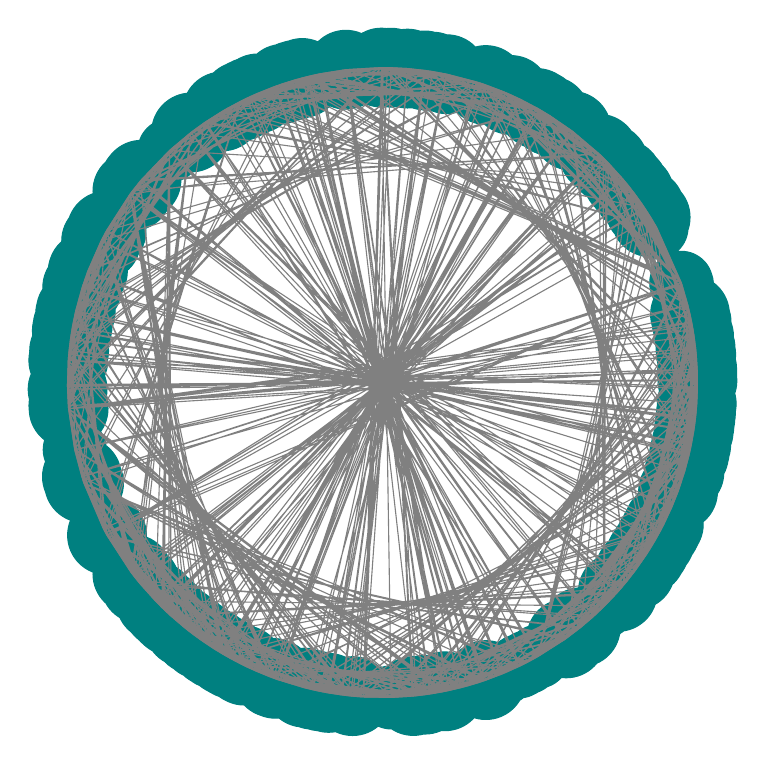
\begin{tikzpicture}
\filldraw[fill=teal, draw=teal]
(0.0,4.0) circle (0.4)(0.012271827051863905,3.9999811752383048) circle (0.4)(0.0613568251399524,3.9995293898168502) circle (0.30000000000000004)(3.9995293898168502,-0.061356825139952394) circle (0.4)(3.999077621404861,-0.08589632110187793) circle (0.4)(0.11043258311586296,3.9984752899807146) circle (0.5)(-0.24528294520883298,-3.9924724516005967) circle (0.4)(3.9908922665767665,-0.2697756782546559) circle (0.5)(-3.990045824561214,0.282018293558456) circle (0.5)(0.3187297518857205,3.9872811971646627) circle (0.5)(-0.3187297518857198,-3.987281197164663) circle (0.4)(-3.9841788036050083,0.355414210330096) circle (0.4)(-0.37985398131855463,-3.9819230219677078) circle (0.5)(3.9807389066887877,-0.3920685613182426) circle (0.5)(-3.9795173231792225,0.4042794510193105) circle (0.5)(-0.40427945101931073,-3.9795173231792225) circle (0.4)(-0.440888829175532,-3.9756278800094242) circle (0.4)(3.974256542082381,-0.45308380871025694) circle (0.5)(3.9714016578394604,-0.4774608592439649) circle (0.4)(-0.5139924431751713,-3.966839014676398) circle (0.30000000000000004)(-0.5261601148115324,-3.9652434393844618) circle (0.4)(0.5383228340285047,3.96361054171112) circle (0.5)(-3.961940337025828,0.5504804863459447) circle (0.4)(3.961940337025828,-0.5504804863459443) circle (0.5)(3.953030270922998,-0.6111887410337732) circle (0.5)(3.9511365665782887,-0.6233135906170608) circle (0.5)(0.6354325733354458,3.9492056726314337) circle (0.5)(-3.945232388978395,0.6596524819598776) circle (0.5)(-0.6838475550412039,-3.9411105695557653) circle (0.5)(-0.7080168816485948,-3.9368403695477165) circle (0.4)(-3.934649676846921,0.7200916056227988) circle (0.5)(3.9207285438724697,-0.7923936428718145) circle (0.5)(-0.7923936428718142,-3.9207285438724697) circle (0.5)(0.8164358643712675,3.915792701276249) circle (0.5)(3.9028085201541143,-0.8764049606274786) circle (0.5)(-3.9028085201541143,0.876404960627479) circle (0.5)(-0.8883744838928137,-3.9001013802679765) circle (0.5)(3.8973575311423034,-0.9003356454391707) circle (0.4)(-3.894576998603248,0.912288332683543) circle (0.5)(3.8917598088222407,-0.9242324331226845) circle (0.5)(-0.9957104229828795,-3.8740883770976695) circle (0.5)(3.8348138995834864,-1.1376301488450868) circle (0.5)(1.196319305232162,3.8169123804364227) circle (0.4)(-3.813224161416775,1.2080237972769126) circle (0.5)(1.243068610998446,3.801944295797927) circle (0.4)(1.31283937431637,3.778419349045921) circle (0.5)(-1.3359986057680364,-3.770292790405788) circle (0.4)(-1.3591075376273072,-3.7620242823730736) circle (0.5)(3.7536141362524327,-1.3821652998559562) circle (0.5)(-1.3936747209977383,-3.7493560476503) circle (0.5)(-3.745062668681114,1.4051710243422662) circle (0.5)(-3.740734039755791,1.4166541016819603) circle (0.5)(-1.4281238449337204,-3.7363702016170355) circle (0.4)(1.5307337294603591,3.695518130045147) circle (0.30000000000000004)(3.671603102485562,-1.5872399496668412) circle (0.4)(-1.6097386034376733,-3.6617948643530713) circle (0.4)(1.6097386034376737,3.6617948643530713) circle (0.4)(1.6321766514599148,3.651848761713593) circle (0.5)(-1.7213059253603307,-3.6106932729490353) circle (0.4)(-1.7544649541541093,-3.594697862775816) circle (0.5)(1.7544649541541106,3.5946978627758153) circle (0.4)(-1.7764885782817164,-3.583864999024741) circle (0.5)(-3.5728972047820613,1.7984453186184264) circle (0.5)(3.572897204782061,-1.7984453186184268) circle (0.5)(3.5448901205955226,-1.8530391342074406) circle (0.5)(3.52768505739342,-1.8855869473039908) circle (0.5)(-1.9179750306406123,-3.510181160829045) circle (0.5)(-3.5042803767816277,1.9287350883164889) circle (0.5)(-1.9502006405937427,-3.492379913673161) circle (0.5)(1.9609059331531646,3.486380346623804) circle (0.5)(1.9929106678911275,3.4681849820627706) circle (0.5)(3.4620544963622764,-2.0035415304449633) circle (0.5)(-2.003541530444963,-3.4620544963622764) circle (0.5)(2.0141535349028703,3.4558914244863472) circle (0.5)(-2.02474658138062,-3.449695824444163) circle (0.4)(-2.0353205701724284,-3.4434677545510692) circle (0.4)(-2.045875401751881,-3.437207273428034) circle (0.4)(3.392481379213189,-2.119214498745179) circle (0.5)(2.1296125115087916,3.3859637550962085) circle (0.5)(-2.129612511508791,-3.3859637550962085) circle (0.5)(-2.1812999536881845,-3.3528988222193528) circle (0.5)(3.346190908894048,-2.1915762366924008) circle (0.5)(-2.273035810680526,-3.2913991255033057) circle (0.4)(-2.313255185646622,-3.2632576432269356) circle (0.5)(3.2128301259225798,-2.3827972179697334) circle (0.5)(-3.2055046868925614,2.392642827985368) circle (0.4)(-2.4024659175354746,-3.198149076431621) circle (0.5)(2.402465917535476,3.19814907643162) circle (0.5)(2.422044165617302,3.1833476184355343) circle (0.4)(-3.1759019102173482,2.431799139871095) circle (0.5)(-2.470589231751215,-3.1458208543963435) circle (0.4)(-2.518552955659708,-3.1075538626929298) circle (0.5)(3.1075538626929298,-2.5185529556597084) circle (0.4)(-3.076413350582319,2.5564977794551025) circle (0.5)(-3.0606690624898367,2.5753261715591647) circle (0.5)(3.0288353860259387,-2.612691371815106) circle (0.4)(2.9884024239207205,-2.6588439128133796) circle (0.5)(2.9720318085404873,-2.6771303533865436) circle (0.4)(-2.6862358193880738,-2.9638045014198364) circle (0.5)(-2.713400172519445,-2.938955512383855) circle (0.5)(2.749261363567036,2.905436620337384) circle (0.5)(-2.775885843558615,-2.8800100318455275) circle (0.5)(-2.793504997635891,-2.862923301135275) circle (0.5)(-2.802275175772993,-2.854339475123175) circle (0.4)(2.8022751757729933,2.8543394751231745) circle (0.4)(2.8370913057554628,2.81973632150362) circle (0.4)(2.81973632150362,-2.837091305755462) circle (0.4)(2.871480180222927,2.784708525965852) circle (0.5)(-2.8800100318455266,-2.775885843558616) circle (0.5)(-2.704370814301264,2.947266275509479) circle (0.4)(2.686235819388074,-2.9638045014198355) circle (0.4)(2.65884391281338,-2.98840242392072) circle (0.4)(3.052753669053525,2.5847040519332656) circle (0.5)(-3.076413350582318,-2.556497779455104) circle (0.5)(2.518552955659709,-3.1075538626929293) circle (0.5)(-3.1152660495259026,-2.5090072619805777) circle (0.4)(2.5090072619805763,-3.115266049525904) circle (0.30000000000000004)(3.1229489142883775,2.499437952569546) circle (0.5)(-3.145820854396343,-2.470589231751216) circle (0.4)(-3.1759019102173474,-2.4317991398710963) circle (0.5)(-2.4317991398710963,3.1759019102173474) circle (0.5)(3.19814907643162,2.402465917535476) circle (0.5)(-3.198149076431619,-2.4024659175354772) circle (0.4)(2.333234611750794,-3.249002346340815) circle (0.5)(2.313255185646623,-3.263257643226935) circle (0.4)(3.2773900803071876,2.2931886667921693) circle (0.4)(-2.2629272431344543,3.2983572111401003) circle (0.4)(-2.2426463047893463,3.3121801810310214) circle (0.2)(3.325878449210181,2.222280932078409) circle (0.4)(3.3326806588076527,2.2120668223201103) circle (0.5)(3.405420772421061,2.0983587307138754) circle (0.5)(-2.0353205701724297,3.4434677545510683) circle (0.5)(1.9715927689191366,-3.4803479644348454) circle (0.4)(3.4803479644348454,1.9715927689191364) circle (0.4)(-1.971592768919137,3.4803479644348454) circle (0.30000000000000004)(-3.4983466091127045,-1.9394769920031647) circle (0.5)(-3.5160489057145337,-1.9071969202532886) circle (0.4)(-3.544890120595522,-1.8530391342074415) circle (0.4)(1.842154843832961,-3.5505584816114153) circle (0.4)(-1.798445318618428,3.5728972047820604) circle (0.5)(1.7544649541541102,-3.5946978627758157) circle (0.4)(1.7323752754126083,-3.6053953881840877) circle (0.4)(-1.732375275412609,3.6053953881840877) circle (0.5)(-1.6880010831991983,3.626382818059662) circle (0.5)(-1.6545532489537407,3.6417651690322677) circle (0.4)(-1.5872399496668432,3.671603102485561) circle (0.5)(1.5307337294603596,-3.695518130045147) circle (0.4)(-1.3706428692479797,3.757836894408759) circle (0.4)(-1.3591075376273085,3.7620242823730727) circle (0.4)(1.3128393743163709,-3.7784193490459206) circle (0.5)(1.2896307152042794,-3.786403652333134) circle (0.4)(-3.790342364070965,-1.2780081232640617) circle (0.5)(1.2780081232640632,-3.7903423640709644) circle (0.2)(3.794245399662921,1.2663735022246634) circle (0.4)(-1.266373502224665,3.7942453996629206) circle (0.5)(3.801944295797927,1.243068610998446) circle (0.4)(1.1963193052321621,-3.8169123804364222) circle (0.4)(-3.8169123804364222,-1.1963193052321623) circle (0.5)(-1.1493898381789174,3.8313056521101316) circle (0.5)(-1.1022872772438337,3.845121943245282) circle (0.5)(1.090485421799797,-3.848485617076166) circle (0.4)(-1.0194626384180576,3.8679058841794087) circle (0.5)(0.9957104229828804,-3.8740883770976695) circle (0.4)(3.877124941426194,0.9838202013431784) circle (0.4)(-0.9600120897949658,3.8830885629158014) circle (0.4)(-0.9361678343341745,3.888905988315745) circle (0.4)(-0.9122883326835447,3.8945769986032475) circle (0.4)(3.9054789253200846,0.8644271883048784) circle (0.5)(0.8524412796643657,-3.908112570631017) circle (0.4)(-3.908112570631017,-0.8524412796643677) circle (0.4)(-0.8164358643712696,3.9157927012762483) circle (0.4)(0.7923936428718152,-3.9207285438724693) circle (0.5)(-0.7923936428718139,3.9207285438724697) circle (0.4)(0.7683215881995699,-3.9255167732550182) circle (0.4)(3.9255167732550182,0.7683215881995696) circle (0.5)(0.7442206066537876,-3.930157209149765) circle (0.4)(3.934649676846921,0.7200916056227981) circle (0.4)(3.9431900366702695,0.6717531798989249) circle (0.4)(0.6111887410337747,-3.953030270922998) circle (0.4)(0.5990581387092858,-3.954886767841295) circle (0.4)(3.956706039859124,0.586921897821447) circle (0.5)(0.5383228340285051,-3.96361054171112) circle (0.5)(-0.46527452364761934,3.972847796939178) circle (0.5)(3.9756278800094242,0.44088882917553274) circle (0.5)(0.42868969982723665,-3.9769617978127516) circle (0.4)(3.9795173231792225,0.4042794510193115) circle (0.4)(0.3920685613182433,-3.9807389066887873) circle (0.5)(0.37985398131855563,-3.9819230219677078) circle (0.4)(3.984178803605008,0.35541421033009873) circle (0.5)(-3.9862845831622193,-0.3309610581975028) circle (0.5)(-3.989161826714761,-0.2942582543986694) circle (0.5)(3.9963109110105814,0.17175302773976384) circle (0.5)(3.997722418221847,0.13496468740551057) circle (0.5)(0.11043258311586264,-3.9984752899807146) circle (0.4)(-3.999077621404861,-0.08589632110187714) circle (0.5)(-3.999698807356578,-0.04908615314288205) circle (0.4)(-3.9998305782078556,-0.03681501912824033) circle (0.4)(3.9998305782078556,0.03681501912823984) circle (0.4)(3.9999247011304044,0.02454353859661806) circle (0.5)(-3.9999247011304044,-0.024543538596617665) circle (0.30000000000000004)(-0.012271827051866175,3.9999811752383048) circle (0.5);
\draw [gray]
(0.0,4.0) -- (0.012271827051863905,3.9999811752383048)
(0.0,4.0) -- (0.0613568251399524,3.9995293898168502)
(0.0,4.0) -- (0.0613568251399524,3.9995293898168502)
(0.0,4.0) -- (0.11043258311586296,3.9984752899807146)
(0.0,4.0) -- (0.3187297518857205,3.9872811971646627)
(0.0,4.0) -- (0.5383228340285047,3.96361054171112)
(0.0,4.0) -- (0.8164358643712675,3.915792701276249)
(0.0,4.0) -- (1.5307337294603591,3.695518130045147)
(0.0,4.0) -- (2.8370913057554628,2.81973632150362)
(0.0,4.0) -- (3.9995293898168502,-0.061356825139952394)
(0.0,4.0) -- (-0.24528294520883298,-3.9924724516005967)
(0.012271827051863905,3.9999811752383048) -- (0.0613568251399524,3.9995293898168502)
(0.012271827051863905,3.9999811752383048) -- (0.0613568251399524,3.9995293898168502)
(0.012271827051863905,3.9999811752383048) -- (0.0613568251399524,3.9995293898168502)
(0.012271827051863905,3.9999811752383048) -- (0.11043258311586296,3.9984752899807146)
(0.012271827051863905,3.9999811752383048) -- (0.3187297518857205,3.9872811971646627)
(0.012271827051863905,3.9999811752383048) -- (0.5383228340285047,3.96361054171112)
(0.012271827051863905,3.9999811752383048) -- (0.8164358643712675,3.915792701276249)
(0.012271827051863905,3.9999811752383048) -- (1.6097386034376737,3.6617948643530713)
(0.012271827051863905,3.9999811752383048) -- (2.8370913057554628,2.81973632150362)
(0.012271827051863905,3.9999811752383048) -- (3.9995293898168502,-0.061356825139952394)
(0.012271827051863905,3.9999811752383048) -- (-0.24528294520883298,-3.9924724516005967)
(0.0613568251399524,3.9995293898168502) -- (0.11043258311586296,3.9984752899807146)
(0.0613568251399524,3.9995293898168502) -- (0.11043258311586296,3.9984752899807146)
(0.0613568251399524,3.9995293898168502) -- (0.11043258311586296,3.9984752899807146)
(0.0613568251399524,3.9995293898168502) -- (0.3187297518857205,3.9872811971646627)
(0.0613568251399524,3.9995293898168502) -- (0.3187297518857205,3.9872811971646627)
(0.0613568251399524,3.9995293898168502) -- (0.5383228340285047,3.96361054171112)
(0.0613568251399524,3.9995293898168502) -- (1.196319305232162,3.8169123804364227)
(0.0613568251399524,3.9995293898168502) -- (1.6097386034376737,3.6617948643530713)
(0.0613568251399524,3.9995293898168502) -- (2.871480180222927,2.784708525965852)
(0.0613568251399524,3.9995293898168502) -- (3.9995293898168502,-0.061356825139952394)
(0.0613568251399524,3.9995293898168502) -- (-0.24528294520883298,-3.9924724516005967)
(3.9995293898168502,-0.061356825139952394) -- (3.999077621404861,-0.08589632110187793)
(3.9995293898168502,-0.061356825139952394) -- (3.999077621404861,-0.08589632110187793)
(3.9995293898168502,-0.061356825139952394) -- (3.9908922665767665,-0.2697756782546559)
(3.9995293898168502,-0.061356825139952394) -- (3.9908922665767665,-0.2697756782546559)
(3.9995293898168502,-0.061356825139952394) -- (3.9908922665767665,-0.2697756782546559)
(3.9995293898168502,-0.061356825139952394) -- (3.974256542082381,-0.45308380871025694)
(3.9995293898168502,-0.061356825139952394) -- (3.9028085201541143,-0.8764049606274786)
(3.9995293898168502,-0.061356825139952394) -- (3.671603102485562,-1.5872399496668412)
(3.9995293898168502,-0.061356825139952394) -- (2.686235819388074,-2.9638045014198355)
(3.9995293898168502,-0.061356825139952394) -- (-0.24528294520883298,-3.9924724516005967)
(3.9995293898168502,-0.061356825139952394) -- (-3.990045824561214,0.282018293558456)
(3.999077621404861,-0.08589632110187793) -- (3.9908922665767665,-0.2697756782546559)
(3.999077621404861,-0.08589632110187793) -- (3.9908922665767665,-0.2697756782546559)
(3.999077621404861,-0.08589632110187793) -- (3.9908922665767665,-0.2697756782546559)
(3.999077621404861,-0.08589632110187793) -- (3.9908922665767665,-0.2697756782546559)
(3.999077621404861,-0.08589632110187793) -- (3.9807389066887877,-0.3920685613182426)
(3.999077621404861,-0.08589632110187793) -- (3.9714016578394604,-0.4774608592439649)
(3.999077621404861,-0.08589632110187793) -- (3.9028085201541143,-0.8764049606274786)
(3.999077621404861,-0.08589632110187793) -- (3.572897204782061,-1.7984453186184268)
(3.999077621404861,-0.08589632110187793) -- (2.686235819388074,-2.9638045014198355)
(3.999077621404861,-0.08589632110187793) -- (-0.24528294520883298,-3.9924724516005967)
(3.999077621404861,-0.08589632110187793) -- (-3.990045824561214,0.282018293558456)
(0.11043258311586296,3.9984752899807146) -- (0.3187297518857205,3.9872811971646627)
(0.11043258311586296,3.9984752899807146) -- (0.3187297518857205,3.9872811971646627)
(0.11043258311586296,3.9984752899807146) -- (0.3187297518857205,3.9872811971646627)
(0.11043258311586296,3.9984752899807146) -- (0.3187297518857205,3.9872811971646627)
(0.11043258311586296,3.9984752899807146) -- (0.3187297518857205,3.9872811971646627)
(0.11043258311586296,3.9984752899807146) -- (0.5383228340285047,3.96361054171112)
(0.11043258311586296,3.9984752899807146) -- (1.196319305232162,3.8169123804364227)
(0.11043258311586296,3.9984752899807146) -- (1.6321766514599148,3.651848761713593)
(0.11043258311586296,3.9984752899807146) -- (3.052753669053525,2.5847040519332656)
(0.11043258311586296,3.9984752899807146) -- (3.9908922665767665,-0.2697756782546559)
(0.11043258311586296,3.9984752899807146) -- (-0.24528294520883298,-3.9924724516005967)
(-0.24528294520883298,-3.9924724516005967) -- (-0.3187297518857198,-3.987281197164663)
(-0.24528294520883298,-3.9924724516005967) -- (-0.3187297518857198,-3.987281197164663)
(-0.24528294520883298,-3.9924724516005967) -- (-0.3187297518857198,-3.987281197164663)
(-0.24528294520883298,-3.9924724516005967) -- (-0.37985398131855463,-3.9819230219677078)
(-0.24528294520883298,-3.9924724516005967) -- (-0.440888829175532,-3.9756278800094242)
(-0.24528294520883298,-3.9924724516005967) -- (-0.6838475550412039,-3.9411105695557653)
(-0.24528294520883298,-3.9924724516005967) -- (-1.3359986057680364,-3.770292790405788)
(-0.24528294520883298,-3.9924724516005967) -- (-1.7544649541541093,-3.594697862775816)
(-0.24528294520883298,-3.9924724516005967) -- (-3.076413350582318,-2.556497779455104)
(-0.24528294520883298,-3.9924724516005967) -- (-3.990045824561214,0.282018293558456)
(-0.24528294520883298,-3.9924724516005967) -- (0.3187297518857205,3.9872811971646627)
(3.9908922665767665,-0.2697756782546559) -- (3.9807389066887877,-0.3920685613182426)
(3.9908922665767665,-0.2697756782546559) -- (3.9807389066887877,-0.3920685613182426)
(3.9908922665767665,-0.2697756782546559) -- (3.9807389066887877,-0.3920685613182426)
(3.9908922665767665,-0.2697756782546559) -- (3.9807389066887877,-0.3920685613182426)
(3.9908922665767665,-0.2697756782546559) -- (3.9714016578394604,-0.4774608592439649)
(3.9908922665767665,-0.2697756782546559) -- (3.9207285438724697,-0.7923936428718145)
(3.9908922665767665,-0.2697756782546559) -- (3.8348138995834864,-1.1376301488450868)
(3.9908922665767665,-0.2697756782546559) -- (3.572897204782061,-1.7984453186184268)
(3.9908922665767665,-0.2697756782546559) -- (2.518552955659709,-3.1075538626929293)
(3.9908922665767665,-0.2697756782546559) -- (-0.3187297518857198,-3.987281197164663)
(3.9908922665767665,-0.2697756782546559) -- (-3.990045824561214,0.282018293558456)
(-3.990045824561214,0.282018293558456) -- (-3.9841788036050083,0.355414210330096)
(-3.990045824561214,0.282018293558456) -- (-3.9841788036050083,0.355414210330096)
(-3.990045824561214,0.282018293558456) -- (-3.9841788036050083,0.355414210330096)
(-3.990045824561214,0.282018293558456) -- (-3.9795173231792225,0.4042794510193105)
(-3.990045824561214,0.282018293558456) -- (-3.961940337025828,0.5504804863459447)
(-3.990045824561214,0.282018293558456) -- (-3.934649676846921,0.7200916056227988)
(-3.990045824561214,0.282018293558456) -- (-3.813224161416775,1.2080237972769126)
(-3.990045824561214,0.282018293558456) -- (-3.5728972047820613,1.7984453186184264)
(-3.990045824561214,0.282018293558456) -- (-2.4317991398710963,3.1759019102173474)
(-3.990045824561214,0.282018293558456) -- (0.3187297518857205,3.9872811971646627)
(-3.990045824561214,0.282018293558456) -- (3.9807389066887877,-0.3920685613182426)
(0.3187297518857205,3.9872811971646627) -- (0.5383228340285047,3.96361054171112)
(0.3187297518857205,3.9872811971646627) -- (0.5383228340285047,3.96361054171112)
(0.3187297518857205,3.9872811971646627) -- (0.5383228340285047,3.96361054171112)
(0.3187297518857205,3.9872811971646627) -- (0.5383228340285047,3.96361054171112)
(0.3187297518857205,3.9872811971646627) -- (0.5383228340285047,3.96361054171112)
(0.3187297518857205,3.9872811971646627) -- (0.8164358643712675,3.915792701276249)
(0.3187297518857205,3.9872811971646627) -- (1.196319305232162,3.8169123804364227)
(0.3187297518857205,3.9872811971646627) -- (1.9609059331531646,3.486380346623804)
(0.3187297518857205,3.9872811971646627) -- (3.052753669053525,2.5847040519332656)
(0.3187297518857205,3.9872811971646627) -- (3.9807389066887877,-0.3920685613182426)
(0.3187297518857205,3.9872811971646627) -- (-0.3187297518857198,-3.987281197164663)
(-0.3187297518857198,-3.987281197164663) -- (-0.37985398131855463,-3.9819230219677078)
(-0.3187297518857198,-3.987281197164663) -- (-0.37985398131855463,-3.9819230219677078)
(-0.3187297518857198,-3.987281197164663) -- (-0.37985398131855463,-3.9819230219677078)
(-0.3187297518857198,-3.987281197164663) -- (-0.440888829175532,-3.9756278800094242)
(-0.3187297518857198,-3.987281197164663) -- (-0.5139924431751713,-3.966839014676398)
(-0.3187297518857198,-3.987281197164663) -- (-0.7080168816485948,-3.9368403695477165)
(-0.3187297518857198,-3.987281197164663) -- (-1.3359986057680364,-3.770292790405788)
(-0.3187297518857198,-3.987281197164663) -- (-1.9179750306406123,-3.510181160829045)
(-0.3187297518857198,-3.987281197164663) -- (-3.076413350582318,-2.556497779455104)
(-0.3187297518857198,-3.987281197164663) -- (-3.9841788036050083,0.355414210330096)
(-0.3187297518857198,-3.987281197164663) -- (0.3187297518857205,3.9872811971646627)
(-3.9841788036050083,0.355414210330096) -- (-3.9795173231792225,0.4042794510193105)
(-3.9841788036050083,0.355414210330096) -- (-3.9795173231792225,0.4042794510193105)
(-3.9841788036050083,0.355414210330096) -- (-3.9795173231792225,0.4042794510193105)
(-3.9841788036050083,0.355414210330096) -- (-3.961940337025828,0.5504804863459447)
(-3.9841788036050083,0.355414210330096) -- (-3.961940337025828,0.5504804863459447)
(-3.9841788036050083,0.355414210330096) -- (-3.9028085201541143,0.876404960627479)
(-3.9841788036050083,0.355414210330096) -- (-3.813224161416775,1.2080237972769126)
(-3.9841788036050083,0.355414210330096) -- (-3.5042803767816277,1.9287350883164889)
(-3.9841788036050083,0.355414210330096) -- (-2.4317991398710963,3.1759019102173474)
(-3.9841788036050083,0.355414210330096) -- (0.5383228340285047,3.96361054171112)
(-3.9841788036050083,0.355414210330096) -- (3.9807389066887877,-0.3920685613182426)
(-0.37985398131855463,-3.9819230219677078) -- (-0.40427945101931073,-3.9795173231792225)
(-0.37985398131855463,-3.9819230219677078) -- (-0.40427945101931073,-3.9795173231792225)
(-0.37985398131855463,-3.9819230219677078) -- (-0.440888829175532,-3.9756278800094242)
(-0.37985398131855463,-3.9819230219677078) -- (-0.5139924431751713,-3.966839014676398)
(-0.37985398131855463,-3.9819230219677078) -- (-0.6838475550412039,-3.9411105695557653)
(-0.37985398131855463,-3.9819230219677078) -- (-0.7923936428718142,-3.9207285438724697)
(-0.37985398131855463,-3.9819230219677078) -- (-1.3359986057680364,-3.770292790405788)
(-0.37985398131855463,-3.9819230219677078) -- (-1.9179750306406123,-3.510181160829045)
(-0.37985398131855463,-3.9819230219677078) -- (-3.1152660495259026,-2.5090072619805777)
(-0.37985398131855463,-3.9819230219677078) -- (-3.9795173231792225,0.4042794510193105)
(-0.37985398131855463,-3.9819230219677078) -- (0.5383228340285047,3.96361054171112)
(3.9807389066887877,-0.3920685613182426) -- (3.974256542082381,-0.45308380871025694)
(3.9807389066887877,-0.3920685613182426) -- (3.974256542082381,-0.45308380871025694)
(3.9807389066887877,-0.3920685613182426) -- (3.974256542082381,-0.45308380871025694)
(3.9807389066887877,-0.3920685613182426) -- (3.961940337025828,-0.5504804863459443)
(3.9807389066887877,-0.3920685613182426) -- (3.953030270922998,-0.6111887410337732)
(3.9807389066887877,-0.3920685613182426) -- (3.9207285438724697,-0.7923936428718145)
(3.9807389066887877,-0.3920685613182426) -- (3.7536141362524327,-1.3821652998559562)
(3.9807389066887877,-0.3920685613182426) -- (3.52768505739342,-1.8855869473039908)
(3.9807389066887877,-0.3920685613182426) -- (2.518552955659709,-3.1075538626929293)
(3.9807389066887877,-0.3920685613182426) -- (-0.40427945101931073,-3.9795173231792225)
(3.9807389066887877,-0.3920685613182426) -- (-3.9795173231792225,0.4042794510193105)
(-3.9795173231792225,0.4042794510193105) -- (-3.961940337025828,0.5504804863459447)
(-3.9795173231792225,0.4042794510193105) -- (-3.961940337025828,0.5504804863459447)
(-3.9795173231792225,0.4042794510193105) -- (-3.961940337025828,0.5504804863459447)
(-3.9795173231792225,0.4042794510193105) -- (-3.961940337025828,0.5504804863459447)
(-3.9795173231792225,0.4042794510193105) -- (-3.945232388978395,0.6596524819598776)
(-3.9795173231792225,0.4042794510193105) -- (-3.9028085201541143,0.876404960627479)
(-3.9795173231792225,0.4042794510193105) -- (-3.813224161416775,1.2080237972769126)
(-3.9795173231792225,0.4042794510193105) -- (-3.5042803767816277,1.9287350883164889)
(-3.9795173231792225,0.4042794510193105) -- (-2.4317991398710963,3.1759019102173474)
(-3.9795173231792225,0.4042794510193105) -- (0.5383228340285047,3.96361054171112)
(-3.9795173231792225,0.4042794510193105) -- (3.974256542082381,-0.45308380871025694)
(-0.40427945101931073,-3.9795173231792225) -- (-0.440888829175532,-3.9756278800094242)
(-0.40427945101931073,-3.9795173231792225) -- (-0.440888829175532,-3.9756278800094242)
(-0.40427945101931073,-3.9795173231792225) -- (-0.5139924431751713,-3.966839014676398)
(-0.40427945101931073,-3.9795173231792225) -- (-0.5139924431751713,-3.966839014676398)
(-0.40427945101931073,-3.9795173231792225) -- (-0.6838475550412039,-3.9411105695557653)
(-0.40427945101931073,-3.9795173231792225) -- (-0.7923936428718142,-3.9207285438724697)
(-0.40427945101931073,-3.9795173231792225) -- (-1.3359986057680364,-3.770292790405788)
(-0.40427945101931073,-3.9795173231792225) -- (-1.9179750306406123,-3.510181160829045)
(-0.40427945101931073,-3.9795173231792225) -- (-3.1152660495259026,-2.5090072619805777)
(-0.40427945101931073,-3.9795173231792225) -- (-3.9795173231792225,0.4042794510193105)
(-0.40427945101931073,-3.9795173231792225) -- (0.5383228340285047,3.96361054171112)
(-0.440888829175532,-3.9756278800094242) -- (-0.5139924431751713,-3.966839014676398)
(-0.440888829175532,-3.9756278800094242) -- (-0.5139924431751713,-3.966839014676398)
(-0.440888829175532,-3.9756278800094242) -- (-0.5139924431751713,-3.966839014676398)
(-0.440888829175532,-3.9756278800094242) -- (-0.6838475550412039,-3.9411105695557653)
(-0.440888829175532,-3.9756278800094242) -- (-0.6838475550412039,-3.9411105695557653)
(-0.440888829175532,-3.9756278800094242) -- (-0.8883744838928137,-3.9001013802679765)
(-0.440888829175532,-3.9756278800094242) -- (-1.3359986057680364,-3.770292790405788)
(-0.440888829175532,-3.9756278800094242) -- (-1.9502006405937427,-3.492379913673161)
(-0.440888829175532,-3.9756278800094242) -- (-3.145820854396343,-2.470589231751216)
(-0.440888829175532,-3.9756278800094242) -- (-3.961940337025828,0.5504804863459447)
(-0.440888829175532,-3.9756278800094242) -- (0.5383228340285047,3.96361054171112)
(3.974256542082381,-0.45308380871025694) -- (3.9714016578394604,-0.4774608592439649)
(3.974256542082381,-0.45308380871025694) -- (3.9714016578394604,-0.4774608592439649)
(3.974256542082381,-0.45308380871025694) -- (3.961940337025828,-0.5504804863459443)
(3.974256542082381,-0.45308380871025694) -- (3.961940337025828,-0.5504804863459443)
(3.974256542082381,-0.45308380871025694) -- (3.9207285438724697,-0.7923936428718145)
(3.974256542082381,-0.45308380871025694) -- (3.9028085201541143,-0.8764049606274786)
(3.974256542082381,-0.45308380871025694) -- (3.7536141362524327,-1.3821652998559562)
(3.974256542082381,-0.45308380871025694) -- (3.4620544963622764,-2.0035415304449633)
(3.974256542082381,-0.45308380871025694) -- (2.333234611750794,-3.249002346340815)
(3.974256542082381,-0.45308380871025694) -- (-0.5139924431751713,-3.966839014676398)
(3.974256542082381,-0.45308380871025694) -- (-3.961940337025828,0.5504804863459447)
(3.9714016578394604,-0.4774608592439649) -- (3.961940337025828,-0.5504804863459443)
(3.9714016578394604,-0.4774608592439649) -- (3.961940337025828,-0.5504804863459443)
(3.9714016578394604,-0.4774608592439649) -- (3.961940337025828,-0.5504804863459443)
(3.9714016578394604,-0.4774608592439649) -- (3.953030270922998,-0.6111887410337732)
(3.9714016578394604,-0.4774608592439649) -- (3.9207285438724697,-0.7923936428718145)
(3.9714016578394604,-0.4774608592439649) -- (3.9028085201541143,-0.8764049606274786)
(3.9714016578394604,-0.4774608592439649) -- (3.7536141362524327,-1.3821652998559562)
(3.9714016578394604,-0.4774608592439649) -- (3.4620544963622764,-2.0035415304449633)
(3.9714016578394604,-0.4774608592439649) -- (2.333234611750794,-3.249002346340815)
(3.9714016578394604,-0.4774608592439649) -- (-0.5139924431751713,-3.966839014676398)
(3.9714016578394604,-0.4774608592439649) -- (-3.961940337025828,0.5504804863459447)
(-0.5139924431751713,-3.966839014676398) -- (-0.5261601148115324,-3.9652434393844618)
(-0.5139924431751713,-3.966839014676398) -- (-0.6838475550412039,-3.9411105695557653)
(-0.5139924431751713,-3.966839014676398) -- (-0.6838475550412039,-3.9411105695557653)
(-0.5139924431751713,-3.966839014676398) -- (-0.6838475550412039,-3.9411105695557653)
(-0.5139924431751713,-3.966839014676398) -- (-0.7080168816485948,-3.9368403695477165)
(-0.5139924431751713,-3.966839014676398) -- (-0.9957104229828795,-3.8740883770976695)
(-0.5139924431751713,-3.966839014676398) -- (-1.3359986057680364,-3.770292790405788)
(-0.5139924431751713,-3.966839014676398) -- (-2.003541530444963,-3.4620544963622764)
(-0.5139924431751713,-3.966839014676398) -- (-3.1759019102173474,-2.4317991398710963)
(-0.5139924431751713,-3.966839014676398) -- (-3.961940337025828,0.5504804863459447)
(-0.5139924431751713,-3.966839014676398) -- (0.5383228340285047,3.96361054171112)
(-0.5261601148115324,-3.9652434393844618) -- (-0.6838475550412039,-3.9411105695557653)
(-0.5261601148115324,-3.9652434393844618) -- (-0.6838475550412039,-3.9411105695557653)
(-0.5261601148115324,-3.9652434393844618) -- (-0.6838475550412039,-3.9411105695557653)
(-0.5261601148115324,-3.9652434393844618) -- (-0.6838475550412039,-3.9411105695557653)
(-0.5261601148115324,-3.9652434393844618) -- (-0.7923936428718142,-3.9207285438724697)
(-0.5261601148115324,-3.9652434393844618) -- (-0.9957104229828795,-3.8740883770976695)
(-0.5261601148115324,-3.9652434393844618) -- (-1.3359986057680364,-3.770292790405788)
(-0.5261601148115324,-3.9652434393844618) -- (-2.003541530444963,-3.4620544963622764)
(-0.5261601148115324,-3.9652434393844618) -- (-3.1759019102173474,-2.4317991398710963)
(-0.5261601148115324,-3.9652434393844618) -- (-3.961940337025828,0.5504804863459447)
(-0.5261601148115324,-3.9652434393844618) -- (0.5383228340285047,3.96361054171112)
(0.5383228340285047,3.96361054171112) -- (0.6354325733354458,3.9492056726314337)
(0.5383228340285047,3.96361054171112) -- (0.6354325733354458,3.9492056726314337)
(0.5383228340285047,3.96361054171112) -- (0.6354325733354458,3.9492056726314337)
(0.5383228340285047,3.96361054171112) -- (0.6354325733354458,3.9492056726314337)
(0.5383228340285047,3.96361054171112) -- (0.8164358643712675,3.915792701276249)
(0.5383228340285047,3.96361054171112) -- (1.196319305232162,3.8169123804364227)
(0.5383228340285047,3.96361054171112) -- (1.31283937431637,3.778419349045921)
(0.5383228340285047,3.96361054171112) -- (2.0141535349028703,3.4558914244863472)
(0.5383228340285047,3.96361054171112) -- (3.19814907643162,2.402465917535476)
(0.5383228340285047,3.96361054171112) -- (3.961940337025828,-0.5504804863459443)
(0.5383228340285047,3.96361054171112) -- (-0.6838475550412039,-3.9411105695557653)
(-3.961940337025828,0.5504804863459447) -- (-3.945232388978395,0.6596524819598776)
(-3.961940337025828,0.5504804863459447) -- (-3.945232388978395,0.6596524819598776)
(-3.961940337025828,0.5504804863459447) -- (-3.945232388978395,0.6596524819598776)
(-3.961940337025828,0.5504804863459447) -- (-3.945232388978395,0.6596524819598776)
(-3.961940337025828,0.5504804863459447) -- (-3.9028085201541143,0.876404960627479)
(-3.961940337025828,0.5504804863459447) -- (-3.813224161416775,1.2080237972769126)
(-3.961940337025828,0.5504804863459447) -- (-3.745062668681114,1.4051710243422662)
(-3.961940337025828,0.5504804863459447) -- (-3.2055046868925614,2.392642827985368)
(-3.961940337025828,0.5504804863459447) -- (-2.2629272431344543,3.2983572111401003)
(-3.961940337025828,0.5504804863459447) -- (0.6354325733354458,3.9492056726314337)
(-3.961940337025828,0.5504804863459447) -- (3.961940337025828,-0.5504804863459443)
(3.961940337025828,-0.5504804863459443) -- (3.953030270922998,-0.6111887410337732)
(3.961940337025828,-0.5504804863459443) -- (3.953030270922998,-0.6111887410337732)
(3.961940337025828,-0.5504804863459443) -- (3.953030270922998,-0.6111887410337732)
(3.961940337025828,-0.5504804863459443) -- (3.9207285438724697,-0.7923936428718145)
(3.961940337025828,-0.5504804863459443) -- (3.9207285438724697,-0.7923936428718145)
(3.961940337025828,-0.5504804863459443) -- (3.8348138995834864,-1.1376301488450868)
(3.961940337025828,-0.5504804863459443) -- (3.7536141362524327,-1.3821652998559562)
(3.961940337025828,-0.5504804863459443) -- (3.392481379213189,-2.119214498745179)
(3.961940337025828,-0.5504804863459443) -- (2.333234611750794,-3.249002346340815)
(3.961940337025828,-0.5504804863459443) -- (-0.6838475550412039,-3.9411105695557653)
(3.961940337025828,-0.5504804863459443) -- (-3.961940337025828,0.5504804863459447)
(3.953030270922998,-0.6111887410337732) -- (3.9511365665782887,-0.6233135906170608)
(3.953030270922998,-0.6111887410337732) -- (3.9207285438724697,-0.7923936428718145)
(3.953030270922998,-0.6111887410337732) -- (3.9207285438724697,-0.7923936428718145)
(3.953030270922998,-0.6111887410337732) -- (3.9207285438724697,-0.7923936428718145)
(3.953030270922998,-0.6111887410337732) -- (3.9028085201541143,-0.8764049606274786)
(3.953030270922998,-0.6111887410337732) -- (3.8348138995834864,-1.1376301488450868)
(3.953030270922998,-0.6111887410337732) -- (3.7536141362524327,-1.3821652998559562)
(3.953030270922998,-0.6111887410337732) -- (3.392481379213189,-2.119214498745179)
(3.953030270922998,-0.6111887410337732) -- (2.333234611750794,-3.249002346340815)
(3.953030270922998,-0.6111887410337732) -- (-0.6838475550412039,-3.9411105695557653)
(3.953030270922998,-0.6111887410337732) -- (-3.945232388978395,0.6596524819598776)
(3.9511365665782887,-0.6233135906170608) -- (3.9207285438724697,-0.7923936428718145)
(3.9511365665782887,-0.6233135906170608) -- (3.9207285438724697,-0.7923936428718145)
(3.9511365665782887,-0.6233135906170608) -- (3.9207285438724697,-0.7923936428718145)
(3.9511365665782887,-0.6233135906170608) -- (3.9207285438724697,-0.7923936428718145)
(3.9511365665782887,-0.6233135906170608) -- (3.9028085201541143,-0.8764049606274786)
(3.9511365665782887,-0.6233135906170608) -- (3.8348138995834864,-1.1376301488450868)
(3.9511365665782887,-0.6233135906170608) -- (3.7536141362524327,-1.3821652998559562)
(3.9511365665782887,-0.6233135906170608) -- (3.392481379213189,-2.119214498745179)
(3.9511365665782887,-0.6233135906170608) -- (2.333234611750794,-3.249002346340815)
(3.9511365665782887,-0.6233135906170608) -- (-0.6838475550412039,-3.9411105695557653)
(3.9511365665782887,-0.6233135906170608) -- (-3.945232388978395,0.6596524819598776)
(0.6354325733354458,3.9492056726314337) -- (0.8164358643712675,3.915792701276249)
(0.6354325733354458,3.9492056726314337) -- (0.8164358643712675,3.915792701276249)
(0.6354325733354458,3.9492056726314337) -- (0.8164358643712675,3.915792701276249)
(0.6354325733354458,3.9492056726314337) -- (0.8164358643712675,3.915792701276249)
(0.6354325733354458,3.9492056726314337) -- (1.196319305232162,3.8169123804364227)
(0.6354325733354458,3.9492056726314337) -- (1.196319305232162,3.8169123804364227)
(0.6354325733354458,3.9492056726314337) -- (1.5307337294603591,3.695518130045147)
(0.6354325733354458,3.9492056726314337) -- (2.1296125115087916,3.3859637550962085)
(0.6354325733354458,3.9492056726314337) -- (3.2773900803071876,2.2931886667921693)
(0.6354325733354458,3.9492056726314337) -- (3.9207285438724697,-0.7923936428718145)
(0.6354325733354458,3.9492056726314337) -- (-0.6838475550412039,-3.9411105695557653)
(-3.945232388978395,0.6596524819598776) -- (-3.934649676846921,0.7200916056227988)
(-3.945232388978395,0.6596524819598776) -- (-3.934649676846921,0.7200916056227988)
(-3.945232388978395,0.6596524819598776) -- (-3.934649676846921,0.7200916056227988)
(-3.945232388978395,0.6596524819598776) -- (-3.9028085201541143,0.876404960627479)
(-3.945232388978395,0.6596524819598776) -- (-3.9028085201541143,0.876404960627479)
(-3.945232388978395,0.6596524819598776) -- (-3.813224161416775,1.2080237972769126)
(-3.945232388978395,0.6596524819598776) -- (-3.740734039755791,1.4166541016819603)
(-3.945232388978395,0.6596524819598776) -- (-3.2055046868925614,2.392642827985368)
(-3.945232388978395,0.6596524819598776) -- (-2.2629272431344543,3.2983572111401003)
(-3.945232388978395,0.6596524819598776) -- (0.8164358643712675,3.915792701276249)
(-3.945232388978395,0.6596524819598776) -- (3.9207285438724697,-0.7923936428718145)
(-0.6838475550412039,-3.9411105695557653) -- (-0.7080168816485948,-3.9368403695477165)
(-0.6838475550412039,-3.9411105695557653) -- (-0.7080168816485948,-3.9368403695477165)
(-0.6838475550412039,-3.9411105695557653) -- (-0.7923936428718142,-3.9207285438724697)
(-0.6838475550412039,-3.9411105695557653) -- (-0.7923936428718142,-3.9207285438724697)
(-0.6838475550412039,-3.9411105695557653) -- (-0.8883744838928137,-3.9001013802679765)
(-0.6838475550412039,-3.9411105695557653) -- (-1.3359986057680364,-3.770292790405788)
(-0.6838475550412039,-3.9411105695557653) -- (-1.6097386034376733,-3.6617948643530713)
(-0.6838475550412039,-3.9411105695557653) -- (-2.1812999536881845,-3.3528988222193528)
(-0.6838475550412039,-3.9411105695557653) -- (-3.4983466091127045,-1.9394769920031647)
(-0.6838475550412039,-3.9411105695557653) -- (-3.934649676846921,0.7200916056227988)
(-0.6838475550412039,-3.9411105695557653) -- (0.8164358643712675,3.915792701276249)
(-0.7080168816485948,-3.9368403695477165) -- (-0.7923936428718142,-3.9207285438724697)
(-0.7080168816485948,-3.9368403695477165) -- (-0.7923936428718142,-3.9207285438724697)
(-0.7080168816485948,-3.9368403695477165) -- (-0.7923936428718142,-3.9207285438724697)
(-0.7080168816485948,-3.9368403695477165) -- (-0.8883744838928137,-3.9001013802679765)
(-0.7080168816485948,-3.9368403695477165) -- (-0.9957104229828795,-3.8740883770976695)
(-0.7080168816485948,-3.9368403695477165) -- (-1.3359986057680364,-3.770292790405788)
(-0.7080168816485948,-3.9368403695477165) -- (-1.6097386034376733,-3.6617948643530713)
(-0.7080168816485948,-3.9368403695477165) -- (-2.1812999536881845,-3.3528988222193528)
(-0.7080168816485948,-3.9368403695477165) -- (-3.4983466091127045,-1.9394769920031647)
(-0.7080168816485948,-3.9368403695477165) -- (-3.934649676846921,0.7200916056227988)
(-0.7080168816485948,-3.9368403695477165) -- (0.8164358643712675,3.915792701276249)
(-3.934649676846921,0.7200916056227988) -- (-3.9028085201541143,0.876404960627479)
(-3.934649676846921,0.7200916056227988) -- (-3.9028085201541143,0.876404960627479)
(-3.934649676846921,0.7200916056227988) -- (-3.9028085201541143,0.876404960627479)
(-3.934649676846921,0.7200916056227988) -- (-3.9028085201541143,0.876404960627479)
(-3.934649676846921,0.7200916056227988) -- (-3.894576998603248,0.912288332683543)
(-3.934649676846921,0.7200916056227988) -- (-3.813224161416775,1.2080237972769126)
(-3.934649676846921,0.7200916056227988) -- (-3.5728972047820613,1.7984453186184264)
(-3.934649676846921,0.7200916056227988) -- (-3.2055046868925614,2.392642827985368)
(-3.934649676846921,0.7200916056227988) -- (-2.2629272431344543,3.2983572111401003)
(-3.934649676846921,0.7200916056227988) -- (0.8164358643712675,3.915792701276249)
(-3.934649676846921,0.7200916056227988) -- (3.9207285438724697,-0.7923936428718145)
(3.9207285438724697,-0.7923936428718145) -- (3.9028085201541143,-0.8764049606274786)
(3.9207285438724697,-0.7923936428718145) -- (3.9028085201541143,-0.8764049606274786)
(3.9207285438724697,-0.7923936428718145) -- (3.9028085201541143,-0.8764049606274786)
(3.9207285438724697,-0.7923936428718145) -- (3.8973575311423034,-0.9003356454391707)
(3.9207285438724697,-0.7923936428718145) -- (3.8348138995834864,-1.1376301488450868)
(3.9207285438724697,-0.7923936428718145) -- (3.7536141362524327,-1.3821652998559562)
(3.9207285438724697,-0.7923936428718145) -- (3.671603102485562,-1.5872399496668412)
(3.9207285438724697,-0.7923936428718145) -- (3.2128301259225798,-2.3827972179697334)
(3.9207285438724697,-0.7923936428718145) -- (1.9715927689191366,-3.4803479644348454)
(3.9207285438724697,-0.7923936428718145) -- (-0.7923936428718142,-3.9207285438724697)
(3.9207285438724697,-0.7923936428718145) -- (-3.9028085201541143,0.876404960627479)
(-0.7923936428718142,-3.9207285438724697) -- (-0.8883744838928137,-3.9001013802679765)
(-0.7923936428718142,-3.9207285438724697) -- (-0.8883744838928137,-3.9001013802679765)
(-0.7923936428718142,-3.9207285438724697) -- (-0.8883744838928137,-3.9001013802679765)
(-0.7923936428718142,-3.9207285438724697) -- (-0.8883744838928137,-3.9001013802679765)
(-0.7923936428718142,-3.9207285438724697) -- (-0.9957104229828795,-3.8740883770976695)
(-0.7923936428718142,-3.9207285438724697) -- (-1.3359986057680364,-3.770292790405788)
(-0.7923936428718142,-3.9207285438724697) -- (-1.6097386034376733,-3.6617948643530713)
(-0.7923936428718142,-3.9207285438724697) -- (-2.273035810680526,-3.2913991255033057)
(-0.7923936428718142,-3.9207285438724697) -- (-3.4983466091127045,-1.9394769920031647)
(-0.7923936428718142,-3.9207285438724697) -- (-3.9028085201541143,0.876404960627479)
(-0.7923936428718142,-3.9207285438724697) -- (0.8164358643712675,3.915792701276249)
(0.8164358643712675,3.915792701276249) -- (1.196319305232162,3.8169123804364227)
(0.8164358643712675,3.915792701276249) -- (1.196319305232162,3.8169123804364227)
(0.8164358643712675,3.915792701276249) -- (1.196319305232162,3.8169123804364227)
(0.8164358643712675,3.915792701276249) -- (1.196319305232162,3.8169123804364227)
(0.8164358643712675,3.915792701276249) -- (1.196319305232162,3.8169123804364227)
(0.8164358643712675,3.915792701276249) -- (1.196319305232162,3.8169123804364227)
(0.8164358643712675,3.915792701276249) -- (1.6097386034376737,3.6617948643530713)
(0.8164358643712675,3.915792701276249) -- (2.402465917535476,3.19814907643162)
(0.8164358643712675,3.915792701276249) -- (3.405420772421061,2.0983587307138754)
(0.8164358643712675,3.915792701276249) -- (3.9028085201541143,-0.8764049606274786)
(0.8164358643712675,3.915792701276249) -- (-0.8883744838928137,-3.9001013802679765)
(3.9028085201541143,-0.8764049606274786) -- (3.8973575311423034,-0.9003356454391707)
(3.9028085201541143,-0.8764049606274786) -- (3.8973575311423034,-0.9003356454391707)
(3.9028085201541143,-0.8764049606274786) -- (3.8917598088222407,-0.9242324331226845)
(3.9028085201541143,-0.8764049606274786) -- (3.8348138995834864,-1.1376301488450868)
(3.9028085201541143,-0.8764049606274786) -- (3.8348138995834864,-1.1376301488450868)
(3.9028085201541143,-0.8764049606274786) -- (3.7536141362524327,-1.3821652998559562)
(3.9028085201541143,-0.8764049606274786) -- (3.572897204782061,-1.7984453186184268)
(3.9028085201541143,-0.8764049606274786) -- (3.2128301259225798,-2.3827972179697334)
(3.9028085201541143,-0.8764049606274786) -- (1.9715927689191366,-3.4803479644348454)
(3.9028085201541143,-0.8764049606274786) -- (-0.8883744838928137,-3.9001013802679765)
(3.9028085201541143,-0.8764049606274786) -- (-3.9028085201541143,0.876404960627479)
(-3.9028085201541143,0.876404960627479) -- (-3.894576998603248,0.912288332683543)
(-3.9028085201541143,0.876404960627479) -- (-3.894576998603248,0.912288332683543)
(-3.9028085201541143,0.876404960627479) -- (-3.813224161416775,1.2080237972769126)
(-3.9028085201541143,0.876404960627479) -- (-3.813224161416775,1.2080237972769126)
(-3.9028085201541143,0.876404960627479) -- (-3.813224161416775,1.2080237972769126)
(-3.9028085201541143,0.876404960627479) -- (-3.745062668681114,1.4051710243422662)
(-3.9028085201541143,0.876404960627479) -- (-3.5728972047820613,1.7984453186184264)
(-3.9028085201541143,0.876404960627479) -- (-3.2055046868925614,2.392642827985368)
(-3.9028085201541143,0.876404960627479) -- (-2.0353205701724297,3.4434677545510683)
(-3.9028085201541143,0.876404960627479) -- (1.196319305232162,3.8169123804364227)
(-3.9028085201541143,0.876404960627479) -- (3.9028085201541143,-0.8764049606274786)
(-0.8883744838928137,-3.9001013802679765) -- (-0.9957104229828795,-3.8740883770976695)
(-0.8883744838928137,-3.9001013802679765) -- (-0.9957104229828795,-3.8740883770976695)
(-0.8883744838928137,-3.9001013802679765) -- (-0.9957104229828795,-3.8740883770976695)
(-0.8883744838928137,-3.9001013802679765) -- (-0.9957104229828795,-3.8740883770976695)
(-0.8883744838928137,-3.9001013802679765) -- (-1.3359986057680364,-3.770292790405788)
(-0.8883744838928137,-3.9001013802679765) -- (-1.3359986057680364,-3.770292790405788)
(-0.8883744838928137,-3.9001013802679765) -- (-1.7213059253603307,-3.6106932729490353)
(-0.8883744838928137,-3.9001013802679765) -- (-2.313255185646622,-3.2632576432269356)
(-0.8883744838928137,-3.9001013802679765) -- (-3.4983466091127045,-1.9394769920031647)
(-0.8883744838928137,-3.9001013802679765) -- (-3.894576998603248,0.912288332683543)
(-0.8883744838928137,-3.9001013802679765) -- (1.196319305232162,3.8169123804364227)
(3.8973575311423034,-0.9003356454391707) -- (3.8917598088222407,-0.9242324331226845)
(3.8973575311423034,-0.9003356454391707) -- (3.8917598088222407,-0.9242324331226845)
(3.8973575311423034,-0.9003356454391707) -- (3.8348138995834864,-1.1376301488450868)
(3.8973575311423034,-0.9003356454391707) -- (3.8348138995834864,-1.1376301488450868)
(3.8973575311423034,-0.9003356454391707) -- (3.8348138995834864,-1.1376301488450868)
(3.8973575311423034,-0.9003356454391707) -- (3.7536141362524327,-1.3821652998559562)
(3.8973575311423034,-0.9003356454391707) -- (3.572897204782061,-1.7984453186184268)
(3.8973575311423034,-0.9003356454391707) -- (3.2128301259225798,-2.3827972179697334)
(3.8973575311423034,-0.9003356454391707) -- (1.9715927689191366,-3.4803479644348454)
(3.8973575311423034,-0.9003356454391707) -- (-0.9957104229828795,-3.8740883770976695)
(3.8973575311423034,-0.9003356454391707) -- (-3.894576998603248,0.912288332683543)
(-3.894576998603248,0.912288332683543) -- (-3.813224161416775,1.2080237972769126)
(-3.894576998603248,0.912288332683543) -- (-3.813224161416775,1.2080237972769126)
(-3.894576998603248,0.912288332683543) -- (-3.813224161416775,1.2080237972769126)
(-3.894576998603248,0.912288332683543) -- (-3.813224161416775,1.2080237972769126)
(-3.894576998603248,0.912288332683543) -- (-3.813224161416775,1.2080237972769126)
(-3.894576998603248,0.912288332683543) -- (-3.745062668681114,1.4051710243422662)
(-3.894576998603248,0.912288332683543) -- (-3.5728972047820613,1.7984453186184264)
(-3.894576998603248,0.912288332683543) -- (-3.2055046868925614,2.392642827985368)
(-3.894576998603248,0.912288332683543) -- (-2.0353205701724297,3.4434677545510683)
(-3.894576998603248,0.912288332683543) -- (1.196319305232162,3.8169123804364227)
(-3.894576998603248,0.912288332683543) -- (3.8917598088222407,-0.9242324331226845)
(3.8917598088222407,-0.9242324331226845) -- (3.8348138995834864,-1.1376301488450868)
(3.8917598088222407,-0.9242324331226845) -- (3.8348138995834864,-1.1376301488450868)
(3.8917598088222407,-0.9242324331226845) -- (3.8348138995834864,-1.1376301488450868)
(3.8917598088222407,-0.9242324331226845) -- (3.8348138995834864,-1.1376301488450868)
(3.8917598088222407,-0.9242324331226845) -- (3.8348138995834864,-1.1376301488450868)
(3.8917598088222407,-0.9242324331226845) -- (3.7536141362524327,-1.3821652998559562)
(3.8917598088222407,-0.9242324331226845) -- (3.572897204782061,-1.7984453186184268)
(3.8917598088222407,-0.9242324331226845) -- (3.2128301259225798,-2.3827972179697334)
(3.8917598088222407,-0.9242324331226845) -- (1.9715927689191366,-3.4803479644348454)
(3.8917598088222407,-0.9242324331226845) -- (-0.9957104229828795,-3.8740883770976695)
(3.8917598088222407,-0.9242324331226845) -- (-3.813224161416775,1.2080237972769126)
(-0.9957104229828795,-3.8740883770976695) -- (-1.3359986057680364,-3.770292790405788)
(-0.9957104229828795,-3.8740883770976695) -- (-1.3359986057680364,-3.770292790405788)
(-0.9957104229828795,-3.8740883770976695) -- (-1.3359986057680364,-3.770292790405788)
(-0.9957104229828795,-3.8740883770976695) -- (-1.3359986057680364,-3.770292790405788)
(-0.9957104229828795,-3.8740883770976695) -- (-1.3359986057680364,-3.770292790405788)
(-0.9957104229828795,-3.8740883770976695) -- (-1.3936747209977383,-3.7493560476503)
(-0.9957104229828795,-3.8740883770976695) -- (-1.7544649541541093,-3.594697862775816)
(-0.9957104229828795,-3.8740883770976695) -- (-2.4024659175354746,-3.198149076431621)
(-0.9957104229828795,-3.8740883770976695) -- (-3.4983466091127045,-1.9394769920031647)
(-0.9957104229828795,-3.8740883770976695) -- (-3.813224161416775,1.2080237972769126)
(-0.9957104229828795,-3.8740883770976695) -- (1.196319305232162,3.8169123804364227)
(3.8348138995834864,-1.1376301488450868) -- (3.7536141362524327,-1.3821652998559562)
(3.8348138995834864,-1.1376301488450868) -- (3.7536141362524327,-1.3821652998559562)
(3.8348138995834864,-1.1376301488450868) -- (3.7536141362524327,-1.3821652998559562)
(3.8348138995834864,-1.1376301488450868) -- (3.7536141362524327,-1.3821652998559562)
(3.8348138995834864,-1.1376301488450868) -- (3.7536141362524327,-1.3821652998559562)
(3.8348138995834864,-1.1376301488450868) -- (3.671603102485562,-1.5872399496668412)
(3.8348138995834864,-1.1376301488450868) -- (3.52768505739342,-1.8855869473039908)
(3.8348138995834864,-1.1376301488450868) -- (3.1075538626929298,-2.5185529556597084)
(3.8348138995834864,-1.1376301488450868) -- (1.842154843832961,-3.5505584816114153)
(3.8348138995834864,-1.1376301488450868) -- (-1.3359986057680364,-3.770292790405788)
(3.8348138995834864,-1.1376301488450868) -- (-3.813224161416775,1.2080237972769126)
(1.196319305232162,3.8169123804364227) -- (1.243068610998446,3.801944295797927)
(1.196319305232162,3.8169123804364227) -- (1.243068610998446,3.801944295797927)
(1.196319305232162,3.8169123804364227) -- (1.243068610998446,3.801944295797927)
(1.196319305232162,3.8169123804364227) -- (1.31283937431637,3.778419349045921)
(1.196319305232162,3.8169123804364227) -- (1.5307337294603591,3.695518130045147)
(1.196319305232162,3.8169123804364227) -- (1.6097386034376737,3.6617948643530713)
(1.196319305232162,3.8169123804364227) -- (1.9609059331531646,3.486380346623804)
(1.196319305232162,3.8169123804364227) -- (2.749261363567036,2.905436620337384)
(1.196319305232162,3.8169123804364227) -- (3.794245399662921,1.2663735022246634)
(1.196319305232162,3.8169123804364227) -- (3.7536141362524327,-1.3821652998559562)
(1.196319305232162,3.8169123804364227) -- (-1.3359986057680364,-3.770292790405788)
(-3.813224161416775,1.2080237972769126) -- (-3.745062668681114,1.4051710243422662)
(-3.813224161416775,1.2080237972769126) -- (-3.745062668681114,1.4051710243422662)
(-3.813224161416775,1.2080237972769126) -- (-3.745062668681114,1.4051710243422662)
(-3.813224161416775,1.2080237972769126) -- (-3.745062668681114,1.4051710243422662)
(-3.813224161416775,1.2080237972769126) -- (-3.745062668681114,1.4051710243422662)
(-3.813224161416775,1.2080237972769126) -- (-3.5728972047820613,1.7984453186184264)
(-3.813224161416775,1.2080237972769126) -- (-3.5042803767816277,1.9287350883164889)
(-3.813224161416775,1.2080237972769126) -- (-3.0606690624898367,2.5753261715591647)
(-3.813224161416775,1.2080237972769126) -- (-1.798445318618428,3.5728972047820604)
(-3.813224161416775,1.2080237972769126) -- (1.243068610998446,3.801944295797927)
(-3.813224161416775,1.2080237972769126) -- (3.7536141362524327,-1.3821652998559562)
(1.243068610998446,3.801944295797927) -- (1.31283937431637,3.778419349045921)
(1.243068610998446,3.801944295797927) -- (1.31283937431637,3.778419349045921)
(1.243068610998446,3.801944295797927) -- (1.31283937431637,3.778419349045921)
(1.243068610998446,3.801944295797927) -- (1.5307337294603591,3.695518130045147)
(1.243068610998446,3.801944295797927) -- (1.5307337294603591,3.695518130045147)
(1.243068610998446,3.801944295797927) -- (1.6097386034376737,3.6617948643530713)
(1.243068610998446,3.801944295797927) -- (1.9609059331531646,3.486380346623804)
(1.243068610998446,3.801944295797927) -- (2.749261363567036,2.905436620337384)
(1.243068610998446,3.801944295797927) -- (3.794245399662921,1.2663735022246634)
(1.243068610998446,3.801944295797927) -- (3.7536141362524327,-1.3821652998559562)
(1.243068610998446,3.801944295797927) -- (-1.3359986057680364,-3.770292790405788)
(1.31283937431637,3.778419349045921) -- (1.5307337294603591,3.695518130045147)
(1.31283937431637,3.778419349045921) -- (1.5307337294603591,3.695518130045147)
(1.31283937431637,3.778419349045921) -- (1.5307337294603591,3.695518130045147)
(1.31283937431637,3.778419349045921) -- (1.5307337294603591,3.695518130045147)
(1.31283937431637,3.778419349045921) -- (1.5307337294603591,3.695518130045147)
(1.31283937431637,3.778419349045921) -- (1.7544649541541106,3.5946978627758153)
(1.31283937431637,3.778419349045921) -- (2.1296125115087916,3.3859637550962085)
(1.31283937431637,3.778419349045921) -- (2.749261363567036,2.905436620337384)
(1.31283937431637,3.778419349045921) -- (3.794245399662921,1.2663735022246634)
(1.31283937431637,3.778419349045921) -- (3.7536141362524327,-1.3821652998559562)
(1.31283937431637,3.778419349045921) -- (-1.3359986057680364,-3.770292790405788)
(-1.3359986057680364,-3.770292790405788) -- (-1.3591075376273072,-3.7620242823730736)
(-1.3359986057680364,-3.770292790405788) -- (-1.3591075376273072,-3.7620242823730736)
(-1.3359986057680364,-3.770292790405788) -- (-1.3936747209977383,-3.7493560476503)
(-1.3359986057680364,-3.770292790405788) -- (-1.4281238449337204,-3.7363702016170355)
(-1.3359986057680364,-3.770292790405788) -- (-1.6097386034376733,-3.6617948643530713)
(-1.3359986057680364,-3.770292790405788) -- (-1.7213059253603307,-3.6106932729490353)
(-1.3359986057680364,-3.770292790405788) -- (-2.045875401751881,-3.437207273428034)
(-1.3359986057680364,-3.770292790405788) -- (-2.6862358193880738,-2.9638045014198364)
(-1.3359986057680364,-3.770292790405788) -- (-3.790342364070965,-1.2780081232640617)
(-1.3359986057680364,-3.770292790405788) -- (-3.745062668681114,1.4051710243422662)
(-1.3359986057680364,-3.770292790405788) -- (1.5307337294603591,3.695518130045147)
(-1.3591075376273072,-3.7620242823730736) -- (-1.3936747209977383,-3.7493560476503)
(-1.3591075376273072,-3.7620242823730736) -- (-1.3936747209977383,-3.7493560476503)
(-1.3591075376273072,-3.7620242823730736) -- (-1.4281238449337204,-3.7363702016170355)
(-1.3591075376273072,-3.7620242823730736) -- (-1.6097386034376733,-3.6617948643530713)
(-1.3591075376273072,-3.7620242823730736) -- (-1.6097386034376733,-3.6617948643530713)
(-1.3591075376273072,-3.7620242823730736) -- (-1.7213059253603307,-3.6106932729490353)
(-1.3591075376273072,-3.7620242823730736) -- (-2.129612511508791,-3.3859637550962085)
(-1.3591075376273072,-3.7620242823730736) -- (-2.713400172519445,-2.938955512383855)
(-1.3591075376273072,-3.7620242823730736) -- (-3.790342364070965,-1.2780081232640617)
(-1.3591075376273072,-3.7620242823730736) -- (-3.745062668681114,1.4051710243422662)
(-1.3591075376273072,-3.7620242823730736) -- (1.5307337294603591,3.695518130045147)
(3.7536141362524327,-1.3821652998559562) -- (3.671603102485562,-1.5872399496668412)
(3.7536141362524327,-1.3821652998559562) -- (3.671603102485562,-1.5872399496668412)
(3.7536141362524327,-1.3821652998559562) -- (3.671603102485562,-1.5872399496668412)
(3.7536141362524327,-1.3821652998559562) -- (3.671603102485562,-1.5872399496668412)
(3.7536141362524327,-1.3821652998559562) -- (3.671603102485562,-1.5872399496668412)
(3.7536141362524327,-1.3821652998559562) -- (3.572897204782061,-1.7984453186184268)
(3.7536141362524327,-1.3821652998559562) -- (3.392481379213189,-2.119214498745179)
(3.7536141362524327,-1.3821652998559562) -- (2.81973632150362,-2.837091305755462)
(3.7536141362524327,-1.3821652998559562) -- (1.5307337294603596,-3.695518130045147)
(3.7536141362524327,-1.3821652998559562) -- (-1.3936747209977383,-3.7493560476503)
(3.7536141362524327,-1.3821652998559562) -- (-3.745062668681114,1.4051710243422662)
(-1.3936747209977383,-3.7493560476503) -- (-1.4281238449337204,-3.7363702016170355)
(-1.3936747209977383,-3.7493560476503) -- (-1.4281238449337204,-3.7363702016170355)
(-1.3936747209977383,-3.7493560476503) -- (-1.6097386034376733,-3.6617948643530713)
(-1.3936747209977383,-3.7493560476503) -- (-1.6097386034376733,-3.6617948643530713)
(-1.3936747209977383,-3.7493560476503) -- (-1.6097386034376733,-3.6617948643530713)
(-1.3936747209977383,-3.7493560476503) -- (-1.7544649541541093,-3.594697862775816)
(-1.3936747209977383,-3.7493560476503) -- (-2.129612511508791,-3.3859637550962085)
(-1.3936747209977383,-3.7493560476503) -- (-2.775885843558615,-2.8800100318455275)
(-1.3936747209977383,-3.7493560476503) -- (-3.790342364070965,-1.2780081232640617)
(-1.3936747209977383,-3.7493560476503) -- (-3.745062668681114,1.4051710243422662)
(-1.3936747209977383,-3.7493560476503) -- (1.5307337294603591,3.695518130045147)
(-3.745062668681114,1.4051710243422662) -- (-3.740734039755791,1.4166541016819603)
(-3.745062668681114,1.4051710243422662) -- (-3.5728972047820613,1.7984453186184264)
(-3.745062668681114,1.4051710243422662) -- (-3.5728972047820613,1.7984453186184264)
(-3.745062668681114,1.4051710243422662) -- (-3.5728972047820613,1.7984453186184264)
(-3.745062668681114,1.4051710243422662) -- (-3.5728972047820613,1.7984453186184264)
(-3.745062668681114,1.4051710243422662) -- (-3.5728972047820613,1.7984453186184264)
(-3.745062668681114,1.4051710243422662) -- (-3.2055046868925614,2.392642827985368)
(-3.745062668681114,1.4051710243422662) -- (-2.704370814301264,2.947266275509479)
(-3.745062668681114,1.4051710243422662) -- (-1.6545532489537407,3.6417651690322677)
(-3.745062668681114,1.4051710243422662) -- (1.5307337294603591,3.695518130045147)
(-3.745062668681114,1.4051710243422662) -- (3.671603102485562,-1.5872399496668412)
(-3.740734039755791,1.4166541016819603) -- (-3.5728972047820613,1.7984453186184264)
(-3.740734039755791,1.4166541016819603) -- (-3.5728972047820613,1.7984453186184264)
(-3.740734039755791,1.4166541016819603) -- (-3.5728972047820613,1.7984453186184264)
(-3.740734039755791,1.4166541016819603) -- (-3.5728972047820613,1.7984453186184264)
(-3.740734039755791,1.4166541016819603) -- (-3.5728972047820613,1.7984453186184264)
(-3.740734039755791,1.4166541016819603) -- (-3.5728972047820613,1.7984453186184264)
(-3.740734039755791,1.4166541016819603) -- (-3.2055046868925614,2.392642827985368)
(-3.740734039755791,1.4166541016819603) -- (-2.704370814301264,2.947266275509479)
(-3.740734039755791,1.4166541016819603) -- (-1.5872399496668432,3.671603102485561)
(-3.740734039755791,1.4166541016819603) -- (1.5307337294603591,3.695518130045147)
(-3.740734039755791,1.4166541016819603) -- (3.671603102485562,-1.5872399496668412)
(-1.4281238449337204,-3.7363702016170355) -- (-1.6097386034376733,-3.6617948643530713)
(-1.4281238449337204,-3.7363702016170355) -- (-1.6097386034376733,-3.6617948643530713)
(-1.4281238449337204,-3.7363702016170355) -- (-1.6097386034376733,-3.6617948643530713)
(-1.4281238449337204,-3.7363702016170355) -- (-1.6097386034376733,-3.6617948643530713)
(-1.4281238449337204,-3.7363702016170355) -- (-1.6097386034376733,-3.6617948643530713)
(-1.4281238449337204,-3.7363702016170355) -- (-1.9179750306406123,-3.510181160829045)
(-1.4281238449337204,-3.7363702016170355) -- (-2.129612511508791,-3.3859637550962085)
(-1.4281238449337204,-3.7363702016170355) -- (-2.775885843558615,-2.8800100318455275)
(-1.4281238449337204,-3.7363702016170355) -- (-3.790342364070965,-1.2780081232640617)
(-1.4281238449337204,-3.7363702016170355) -- (-3.5728972047820613,1.7984453186184264)
(-1.4281238449337204,-3.7363702016170355) -- (1.5307337294603591,3.695518130045147)
(1.5307337294603591,3.695518130045147) -- (1.6097386034376737,3.6617948643530713)
(1.5307337294603591,3.695518130045147) -- (1.6097386034376737,3.6617948643530713)
(1.5307337294603591,3.695518130045147) -- (1.6097386034376737,3.6617948643530713)
(1.5307337294603591,3.695518130045147) -- (1.6321766514599148,3.651848761713593)
(1.5307337294603591,3.695518130045147) -- (1.7544649541541106,3.5946978627758153)
(1.5307337294603591,3.695518130045147) -- (1.9609059331531646,3.486380346623804)
(1.5307337294603591,3.695518130045147) -- (2.402465917535476,3.19814907643162)
(1.5307337294603591,3.695518130045147) -- (2.8370913057554628,2.81973632150362)
(1.5307337294603591,3.695518130045147) -- (3.794245399662921,1.2663735022246634)
(1.5307337294603591,3.695518130045147) -- (3.671603102485562,-1.5872399496668412)
(1.5307337294603591,3.695518130045147) -- (-1.6097386034376733,-3.6617948643530713)
(3.671603102485562,-1.5872399496668412) -- (3.572897204782061,-1.7984453186184268)
(3.671603102485562,-1.5872399496668412) -- (3.572897204782061,-1.7984453186184268)
(3.671603102485562,-1.5872399496668412) -- (3.572897204782061,-1.7984453186184268)
(3.671603102485562,-1.5872399496668412) -- (3.572897204782061,-1.7984453186184268)
(3.671603102485562,-1.5872399496668412) -- (3.572897204782061,-1.7984453186184268)
(3.671603102485562,-1.5872399496668412) -- (3.4620544963622764,-2.0035415304449633)
(3.671603102485562,-1.5872399496668412) -- (3.2128301259225798,-2.3827972179697334)
(3.671603102485562,-1.5872399496668412) -- (2.686235819388074,-2.9638045014198355)
(3.671603102485562,-1.5872399496668412) -- (1.3128393743163709,-3.7784193490459206)
(3.671603102485562,-1.5872399496668412) -- (-1.6097386034376733,-3.6617948643530713)
(3.671603102485562,-1.5872399496668412) -- (-3.5728972047820613,1.7984453186184264)
(-1.6097386034376733,-3.6617948643530713) -- (-1.7213059253603307,-3.6106932729490353)
(-1.6097386034376733,-3.6617948643530713) -- (-1.7213059253603307,-3.6106932729490353)
(-1.6097386034376733,-3.6617948643530713) -- (-1.7213059253603307,-3.6106932729490353)
(-1.6097386034376733,-3.6617948643530713) -- (-1.7213059253603307,-3.6106932729490353)
(-1.6097386034376733,-3.6617948643530713) -- (-1.9179750306406123,-3.510181160829045)
(-1.6097386034376733,-3.6617948643530713) -- (-2.003541530444963,-3.4620544963622764)
(-1.6097386034376733,-3.6617948643530713) -- (-2.313255185646622,-3.2632576432269356)
(-1.6097386034376733,-3.6617948643530713) -- (-3.076413350582318,-2.556497779455104)
(-1.6097386034376733,-3.6617948643530713) -- (-3.790342364070965,-1.2780081232640617)
(-1.6097386034376733,-3.6617948643530713) -- (-3.5728972047820613,1.7984453186184264)
(-1.6097386034376733,-3.6617948643530713) -- (1.6097386034376737,3.6617948643530713)
(1.6097386034376737,3.6617948643530713) -- (1.6321766514599148,3.651848761713593)
(1.6097386034376737,3.6617948643530713) -- (1.6321766514599148,3.651848761713593)
(1.6097386034376737,3.6617948643530713) -- (1.7544649541541106,3.5946978627758153)
(1.6097386034376737,3.6617948643530713) -- (1.7544649541541106,3.5946978627758153)
(1.6097386034376737,3.6617948643530713) -- (1.9609059331531646,3.486380346623804)
(1.6097386034376737,3.6617948643530713) -- (1.9609059331531646,3.486380346623804)
(1.6097386034376737,3.6617948643530713) -- (2.402465917535476,3.19814907643162)
(1.6097386034376737,3.6617948643530713) -- (3.052753669053525,2.5847040519332656)
(1.6097386034376737,3.6617948643530713) -- (3.794245399662921,1.2663735022246634)
(1.6097386034376737,3.6617948643530713) -- (3.572897204782061,-1.7984453186184268)
(1.6097386034376737,3.6617948643530713) -- (-1.6097386034376733,-3.6617948643530713)
(1.6321766514599148,3.651848761713593) -- (1.7544649541541106,3.5946978627758153)
(1.6321766514599148,3.651848761713593) -- (1.7544649541541106,3.5946978627758153)
(1.6321766514599148,3.651848761713593) -- (1.7544649541541106,3.5946978627758153)
(1.6321766514599148,3.651848761713593) -- (1.7544649541541106,3.5946978627758153)
(1.6321766514599148,3.651848761713593) -- (1.9609059331531646,3.486380346623804)
(1.6321766514599148,3.651848761713593) -- (1.9929106678911275,3.4681849820627706)
(1.6321766514599148,3.651848761713593) -- (2.402465917535476,3.19814907643162)
(1.6321766514599148,3.651848761713593) -- (3.052753669053525,2.5847040519332656)
(1.6321766514599148,3.651848761713593) -- (3.794245399662921,1.2663735022246634)
(1.6321766514599148,3.651848761713593) -- (3.572897204782061,-1.7984453186184268)
(1.6321766514599148,3.651848761713593) -- (-1.7213059253603307,-3.6106932729490353)
(-1.7213059253603307,-3.6106932729490353) -- (-1.7544649541541093,-3.594697862775816)
(-1.7213059253603307,-3.6106932729490353) -- (-1.7544649541541093,-3.594697862775816)
(-1.7213059253603307,-3.6106932729490353) -- (-1.7764885782817164,-3.583864999024741)
(-1.7213059253603307,-3.6106932729490353) -- (-1.9179750306406123,-3.510181160829045)
(-1.7213059253603307,-3.6106932729490353) -- (-1.9179750306406123,-3.510181160829045)
(-1.7213059253603307,-3.6106932729490353) -- (-2.129612511508791,-3.3859637550962085)
(-1.7213059253603307,-3.6106932729490353) -- (-2.4024659175354746,-3.198149076431621)
(-1.7213059253603307,-3.6106932729490353) -- (-3.076413350582318,-2.556497779455104)
(-1.7213059253603307,-3.6106932729490353) -- (-3.790342364070965,-1.2780081232640617)
(-1.7213059253603307,-3.6106932729490353) -- (-3.5728972047820613,1.7984453186184264)
(-1.7213059253603307,-3.6106932729490353) -- (1.7544649541541106,3.5946978627758153)
(-1.7544649541541093,-3.594697862775816) -- (-1.7764885782817164,-3.583864999024741)
(-1.7544649541541093,-3.594697862775816) -- (-1.7764885782817164,-3.583864999024741)
(-1.7544649541541093,-3.594697862775816) -- (-1.9179750306406123,-3.510181160829045)
(-1.7544649541541093,-3.594697862775816) -- (-1.9179750306406123,-3.510181160829045)
(-1.7544649541541093,-3.594697862775816) -- (-1.9502006405937427,-3.492379913673161)
(-1.7544649541541093,-3.594697862775816) -- (-2.129612511508791,-3.3859637550962085)
(-1.7544649541541093,-3.594697862775816) -- (-2.470589231751215,-3.1458208543963435)
(-1.7544649541541093,-3.594697862775816) -- (-3.076413350582318,-2.556497779455104)
(-1.7544649541541093,-3.594697862775816) -- (-3.790342364070965,-1.2780081232640617)
(-1.7544649541541093,-3.594697862775816) -- (-3.5728972047820613,1.7984453186184264)
(-1.7544649541541093,-3.594697862775816) -- (1.7544649541541106,3.5946978627758153)
(1.7544649541541106,3.5946978627758153) -- (1.9609059331531646,3.486380346623804)
(1.7544649541541106,3.5946978627758153) -- (1.9609059331531646,3.486380346623804)
(1.7544649541541106,3.5946978627758153) -- (1.9609059331531646,3.486380346623804)
(1.7544649541541106,3.5946978627758153) -- (1.9609059331531646,3.486380346623804)
(1.7544649541541106,3.5946978627758153) -- (1.9609059331531646,3.486380346623804)
(1.7544649541541106,3.5946978627758153) -- (2.1296125115087916,3.3859637550962085)
(1.7544649541541106,3.5946978627758153) -- (2.422044165617302,3.1833476184355343)
(1.7544649541541106,3.5946978627758153) -- (3.052753669053525,2.5847040519332656)
(1.7544649541541106,3.5946978627758153) -- (3.794245399662921,1.2663735022246634)
(1.7544649541541106,3.5946978627758153) -- (3.572897204782061,-1.7984453186184268)
(1.7544649541541106,3.5946978627758153) -- (-1.7544649541541093,-3.594697862775816)
(-1.7764885782817164,-3.583864999024741) -- (-1.9179750306406123,-3.510181160829045)
(-1.7764885782817164,-3.583864999024741) -- (-1.9179750306406123,-3.510181160829045)
(-1.7764885782817164,-3.583864999024741) -- (-1.9179750306406123,-3.510181160829045)
(-1.7764885782817164,-3.583864999024741) -- (-1.9179750306406123,-3.510181160829045)
(-1.7764885782817164,-3.583864999024741) -- (-1.9502006405937427,-3.492379913673161)
(-1.7764885782817164,-3.583864999024741) -- (-2.129612511508791,-3.3859637550962085)
(-1.7764885782817164,-3.583864999024741) -- (-2.470589231751215,-3.1458208543963435)
(-1.7764885782817164,-3.583864999024741) -- (-3.076413350582318,-2.556497779455104)
(-1.7764885782817164,-3.583864999024741) -- (-3.790342364070965,-1.2780081232640617)
(-1.7764885782817164,-3.583864999024741) -- (-3.5728972047820613,1.7984453186184264)
(-1.7764885782817164,-3.583864999024741) -- (1.9609059331531646,3.486380346623804)
(-3.5728972047820613,1.7984453186184264) -- (-3.5042803767816277,1.9287350883164889)
(-3.5728972047820613,1.7984453186184264) -- (-3.5042803767816277,1.9287350883164889)
(-3.5728972047820613,1.7984453186184264) -- (-3.5042803767816277,1.9287350883164889)
(-3.5728972047820613,1.7984453186184264) -- (-3.5042803767816277,1.9287350883164889)
(-3.5728972047820613,1.7984453186184264) -- (-3.2055046868925614,2.392642827985368)
(-3.5728972047820613,1.7984453186184264) -- (-3.2055046868925614,2.392642827985368)
(-3.5728972047820613,1.7984453186184264) -- (-3.076413350582319,2.5564977794551025)
(-3.5728972047820613,1.7984453186184264) -- (-2.4317991398710963,3.1759019102173474)
(-3.5728972047820613,1.7984453186184264) -- (-1.1493898381789174,3.8313056521101316)
(-3.5728972047820613,1.7984453186184264) -- (1.9609059331531646,3.486380346623804)
(-3.5728972047820613,1.7984453186184264) -- (3.572897204782061,-1.7984453186184268)
(3.572897204782061,-1.7984453186184268) -- (3.5448901205955226,-1.8530391342074406)
(3.572897204782061,-1.7984453186184268) -- (3.5448901205955226,-1.8530391342074406)
(3.572897204782061,-1.7984453186184268) -- (3.5448901205955226,-1.8530391342074406)
(3.572897204782061,-1.7984453186184268) -- (3.52768505739342,-1.8855869473039908)
(3.572897204782061,-1.7984453186184268) -- (3.4620544963622764,-2.0035415304449633)
(3.572897204782061,-1.7984453186184268) -- (3.346190908894048,-2.1915762366924008)
(3.572897204782061,-1.7984453186184268) -- (3.1075538626929298,-2.5185529556597084)
(3.572897204782061,-1.7984453186184268) -- (2.518552955659709,-3.1075538626929293)
(3.572897204782061,-1.7984453186184268) -- (1.1963193052321621,-3.8169123804364222)
(3.572897204782061,-1.7984453186184268) -- (-1.9179750306406123,-3.510181160829045)
(3.572897204782061,-1.7984453186184268) -- (-3.5728972047820613,1.7984453186184264)
(3.5448901205955226,-1.8530391342074406) -- (3.52768505739342,-1.8855869473039908)
(3.5448901205955226,-1.8530391342074406) -- (3.52768505739342,-1.8855869473039908)
(3.5448901205955226,-1.8530391342074406) -- (3.4620544963622764,-2.0035415304449633)
(3.5448901205955226,-1.8530391342074406) -- (3.4620544963622764,-2.0035415304449633)
(3.5448901205955226,-1.8530391342074406) -- (3.392481379213189,-2.119214498745179)
(3.5448901205955226,-1.8530391342074406) -- (3.346190908894048,-2.1915762366924008)
(3.5448901205955226,-1.8530391342074406) -- (3.1075538626929298,-2.5185529556597084)
(3.5448901205955226,-1.8530391342074406) -- (2.518552955659709,-3.1075538626929293)
(3.5448901205955226,-1.8530391342074406) -- (1.1963193052321621,-3.8169123804364222)
(3.5448901205955226,-1.8530391342074406) -- (-1.9179750306406123,-3.510181160829045)
(3.5448901205955226,-1.8530391342074406) -- (-3.5042803767816277,1.9287350883164889)
(3.52768505739342,-1.8855869473039908) -- (3.4620544963622764,-2.0035415304449633)
(3.52768505739342,-1.8855869473039908) -- (3.4620544963622764,-2.0035415304449633)
(3.52768505739342,-1.8855869473039908) -- (3.4620544963622764,-2.0035415304449633)
(3.52768505739342,-1.8855869473039908) -- (3.4620544963622764,-2.0035415304449633)
(3.52768505739342,-1.8855869473039908) -- (3.392481379213189,-2.119214498745179)
(3.52768505739342,-1.8855869473039908) -- (3.2128301259225798,-2.3827972179697334)
(3.52768505739342,-1.8855869473039908) -- (3.0288353860259387,-2.612691371815106)
(3.52768505739342,-1.8855869473039908) -- (2.518552955659709,-3.1075538626929293)
(3.52768505739342,-1.8855869473039908) -- (1.090485421799797,-3.848485617076166)
(3.52768505739342,-1.8855869473039908) -- (-1.9179750306406123,-3.510181160829045)
(3.52768505739342,-1.8855869473039908) -- (-3.5042803767816277,1.9287350883164889)
(-1.9179750306406123,-3.510181160829045) -- (-1.9502006405937427,-3.492379913673161)
(-1.9179750306406123,-3.510181160829045) -- (-1.9502006405937427,-3.492379913673161)
(-1.9179750306406123,-3.510181160829045) -- (-2.003541530444963,-3.4620544963622764)
(-1.9179750306406123,-3.510181160829045) -- (-2.003541530444963,-3.4620544963622764)
(-1.9179750306406123,-3.510181160829045) -- (-2.129612511508791,-3.3859637550962085)
(-1.9179750306406123,-3.510181160829045) -- (-2.273035810680526,-3.2913991255033057)
(-1.9179750306406123,-3.510181160829045) -- (-2.6862358193880738,-2.9638045014198364)
(-1.9179750306406123,-3.510181160829045) -- (-3.1152660495259026,-2.5090072619805777)
(-1.9179750306406123,-3.510181160829045) -- (-3.908112570631017,-0.8524412796643677)
(-1.9179750306406123,-3.510181160829045) -- (-3.5042803767816277,1.9287350883164889)
(-1.9179750306406123,-3.510181160829045) -- (1.9609059331531646,3.486380346623804)
(-3.5042803767816277,1.9287350883164889) -- (-3.2055046868925614,2.392642827985368)
(-3.5042803767816277,1.9287350883164889) -- (-3.2055046868925614,2.392642827985368)
(-3.5042803767816277,1.9287350883164889) -- (-3.2055046868925614,2.392642827985368)
(-3.5042803767816277,1.9287350883164889) -- (-3.2055046868925614,2.392642827985368)
(-3.5042803767816277,1.9287350883164889) -- (-3.2055046868925614,2.392642827985368)
(-3.5042803767816277,1.9287350883164889) -- (-3.2055046868925614,2.392642827985368)
(-3.5042803767816277,1.9287350883164889) -- (-3.0606690624898367,2.5753261715591647)
(-3.5042803767816277,1.9287350883164889) -- (-2.4317991398710963,3.1759019102173474)
(-3.5042803767816277,1.9287350883164889) -- (-1.1022872772438337,3.845121943245282)
(-3.5042803767816277,1.9287350883164889) -- (1.9609059331531646,3.486380346623804)
(-3.5042803767816277,1.9287350883164889) -- (3.4620544963622764,-2.0035415304449633)
(-1.9502006405937427,-3.492379913673161) -- (-2.003541530444963,-3.4620544963622764)
(-1.9502006405937427,-3.492379913673161) -- (-2.003541530444963,-3.4620544963622764)
(-1.9502006405937427,-3.492379913673161) -- (-2.003541530444963,-3.4620544963622764)
(-1.9502006405937427,-3.492379913673161) -- (-2.0353205701724284,-3.4434677545510692)
(-1.9502006405937427,-3.492379913673161) -- (-2.129612511508791,-3.3859637550962085)
(-1.9502006405937427,-3.492379913673161) -- (-2.313255185646622,-3.2632576432269356)
(-1.9502006405937427,-3.492379913673161) -- (-2.6862358193880738,-2.9638045014198364)
(-1.9502006405937427,-3.492379913673161) -- (-3.145820854396343,-2.470589231751216)
(-1.9502006405937427,-3.492379913673161) -- (-3.908112570631017,-0.8524412796643677)
(-1.9502006405937427,-3.492379913673161) -- (-3.2055046868925614,2.392642827985368)
(-1.9502006405937427,-3.492379913673161) -- (1.9609059331531646,3.486380346623804)
(1.9609059331531646,3.486380346623804) -- (1.9929106678911275,3.4681849820627706)
(1.9609059331531646,3.486380346623804) -- (1.9929106678911275,3.4681849820627706)
(1.9609059331531646,3.486380346623804) -- (2.0141535349028703,3.4558914244863472)
(1.9609059331531646,3.486380346623804) -- (2.1296125115087916,3.3859637550962085)
(1.9609059331531646,3.486380346623804) -- (2.1296125115087916,3.3859637550962085)
(1.9609059331531646,3.486380346623804) -- (2.402465917535476,3.19814907643162)
(1.9609059331531646,3.486380346623804) -- (2.749261363567036,2.905436620337384)
(1.9609059331531646,3.486380346623804) -- (3.19814907643162,2.402465917535476)
(1.9609059331531646,3.486380346623804) -- (3.877124941426194,0.9838202013431784)
(1.9609059331531646,3.486380346623804) -- (3.4620544963622764,-2.0035415304449633)
(1.9609059331531646,3.486380346623804) -- (-2.003541530444963,-3.4620544963622764)
(1.9929106678911275,3.4681849820627706) -- (2.0141535349028703,3.4558914244863472)
(1.9929106678911275,3.4681849820627706) -- (2.0141535349028703,3.4558914244863472)
(1.9929106678911275,3.4681849820627706) -- (2.1296125115087916,3.3859637550962085)
(1.9929106678911275,3.4681849820627706) -- (2.1296125115087916,3.3859637550962085)
(1.9929106678911275,3.4681849820627706) -- (2.402465917535476,3.19814907643162)
(1.9929106678911275,3.4681849820627706) -- (2.402465917535476,3.19814907643162)
(1.9929106678911275,3.4681849820627706) -- (2.749261363567036,2.905436620337384)
(1.9929106678911275,3.4681849820627706) -- (3.19814907643162,2.402465917535476)
(1.9929106678911275,3.4681849820627706) -- (3.877124941426194,0.9838202013431784)
(1.9929106678911275,3.4681849820627706) -- (3.4620544963622764,-2.0035415304449633)
(1.9929106678911275,3.4681849820627706) -- (-2.003541530444963,-3.4620544963622764)
(3.4620544963622764,-2.0035415304449633) -- (3.392481379213189,-2.119214498745179)
(3.4620544963622764,-2.0035415304449633) -- (3.392481379213189,-2.119214498745179)
(3.4620544963622764,-2.0035415304449633) -- (3.392481379213189,-2.119214498745179)
(3.4620544963622764,-2.0035415304449633) -- (3.392481379213189,-2.119214498745179)
(3.4620544963622764,-2.0035415304449633) -- (3.346190908894048,-2.1915762366924008)
(3.4620544963622764,-2.0035415304449633) -- (3.2128301259225798,-2.3827972179697334)
(3.4620544963622764,-2.0035415304449633) -- (2.9884024239207205,-2.6588439128133796)
(3.4620544963622764,-2.0035415304449633) -- (2.333234611750794,-3.249002346340815)
(3.4620544963622764,-2.0035415304449633) -- (0.9957104229828804,-3.8740883770976695)
(3.4620544963622764,-2.0035415304449633) -- (-2.003541530444963,-3.4620544963622764)
(3.4620544963622764,-2.0035415304449633) -- (-3.2055046868925614,2.392642827985368)
(-2.003541530444963,-3.4620544963622764) -- (-2.02474658138062,-3.449695824444163)
(-2.003541530444963,-3.4620544963622764) -- (-2.02474658138062,-3.449695824444163)
(-2.003541530444963,-3.4620544963622764) -- (-2.045875401751881,-3.437207273428034)
(-2.003541530444963,-3.4620544963622764) -- (-2.129612511508791,-3.3859637550962085)
(-2.003541530444963,-3.4620544963622764) -- (-2.1812999536881845,-3.3528988222193528)
(-2.003541530444963,-3.4620544963622764) -- (-2.4024659175354746,-3.198149076431621)
(-2.003541530444963,-3.4620544963622764) -- (-2.6862358193880738,-2.9638045014198364)
(-2.003541530444963,-3.4620544963622764) -- (-3.1759019102173474,-2.4317991398710963)
(-2.003541530444963,-3.4620544963622764) -- (-3.908112570631017,-0.8524412796643677)
(-2.003541530444963,-3.4620544963622764) -- (-3.2055046868925614,2.392642827985368)
(-2.003541530444963,-3.4620544963622764) -- (2.0141535349028703,3.4558914244863472)
(2.0141535349028703,3.4558914244863472) -- (2.1296125115087916,3.3859637550962085)
(2.0141535349028703,3.4558914244863472) -- (2.1296125115087916,3.3859637550962085)
(2.0141535349028703,3.4558914244863472) -- (2.1296125115087916,3.3859637550962085)
(2.0141535349028703,3.4558914244863472) -- (2.1296125115087916,3.3859637550962085)
(2.0141535349028703,3.4558914244863472) -- (2.402465917535476,3.19814907643162)
(2.0141535349028703,3.4558914244863472) -- (2.402465917535476,3.19814907643162)
(2.0141535349028703,3.4558914244863472) -- (2.749261363567036,2.905436620337384)
(2.0141535349028703,3.4558914244863472) -- (3.19814907643162,2.402465917535476)
(2.0141535349028703,3.4558914244863472) -- (3.877124941426194,0.9838202013431784)
(2.0141535349028703,3.4558914244863472) -- (3.392481379213189,-2.119214498745179)
(2.0141535349028703,3.4558914244863472) -- (-2.02474658138062,-3.449695824444163)
(-2.02474658138062,-3.449695824444163) -- (-2.0353205701724284,-3.4434677545510692)
(-2.02474658138062,-3.449695824444163) -- (-2.045875401751881,-3.437207273428034)
(-2.02474658138062,-3.449695824444163) -- (-2.129612511508791,-3.3859637550962085)
(-2.02474658138062,-3.449695824444163) -- (-2.129612511508791,-3.3859637550962085)
(-2.02474658138062,-3.449695824444163) -- (-2.273035810680526,-3.2913991255033057)
(-2.02474658138062,-3.449695824444163) -- (-2.4024659175354746,-3.198149076431621)
(-2.02474658138062,-3.449695824444163) -- (-2.6862358193880738,-2.9638045014198364)
(-2.02474658138062,-3.449695824444163) -- (-3.198149076431619,-2.4024659175354772)
(-2.02474658138062,-3.449695824444163) -- (-3.908112570631017,-0.8524412796643677)
(-2.02474658138062,-3.449695824444163) -- (-3.2055046868925614,2.392642827985368)
(-2.02474658138062,-3.449695824444163) -- (2.1296125115087916,3.3859637550962085)
(-2.0353205701724284,-3.4434677545510692) -- (-2.045875401751881,-3.437207273428034)
(-2.0353205701724284,-3.4434677545510692) -- (-2.129612511508791,-3.3859637550962085)
(-2.0353205701724284,-3.4434677545510692) -- (-2.129612511508791,-3.3859637550962085)
(-2.0353205701724284,-3.4434677545510692) -- (-2.129612511508791,-3.3859637550962085)
(-2.0353205701724284,-3.4434677545510692) -- (-2.273035810680526,-3.2913991255033057)
(-2.0353205701724284,-3.4434677545510692) -- (-2.4024659175354746,-3.198149076431621)
(-2.0353205701724284,-3.4434677545510692) -- (-2.6862358193880738,-2.9638045014198364)
(-2.0353205701724284,-3.4434677545510692) -- (-3.198149076431619,-2.4024659175354772)
(-2.0353205701724284,-3.4434677545510692) -- (-3.908112570631017,-0.8524412796643677)
(-2.0353205701724284,-3.4434677545510692) -- (-3.2055046868925614,2.392642827985368)
(-2.0353205701724284,-3.4434677545510692) -- (2.1296125115087916,3.3859637550962085)
(-2.045875401751881,-3.437207273428034) -- (-2.129612511508791,-3.3859637550962085)
(-2.045875401751881,-3.437207273428034) -- (-2.129612511508791,-3.3859637550962085)
(-2.045875401751881,-3.437207273428034) -- (-2.129612511508791,-3.3859637550962085)
(-2.045875401751881,-3.437207273428034) -- (-2.129612511508791,-3.3859637550962085)
(-2.045875401751881,-3.437207273428034) -- (-2.273035810680526,-3.2913991255033057)
(-2.045875401751881,-3.437207273428034) -- (-2.4024659175354746,-3.198149076431621)
(-2.045875401751881,-3.437207273428034) -- (-2.6862358193880738,-2.9638045014198364)
(-2.045875401751881,-3.437207273428034) -- (-3.4983466091127045,-1.9394769920031647)
(-2.045875401751881,-3.437207273428034) -- (-3.908112570631017,-0.8524412796643677)
(-2.045875401751881,-3.437207273428034) -- (-3.2055046868925614,2.392642827985368)
(-2.045875401751881,-3.437207273428034) -- (2.1296125115087916,3.3859637550962085)
(3.392481379213189,-2.119214498745179) -- (3.346190908894048,-2.1915762366924008)
(3.392481379213189,-2.119214498745179) -- (3.346190908894048,-2.1915762366924008)
(3.392481379213189,-2.119214498745179) -- (3.346190908894048,-2.1915762366924008)
(3.392481379213189,-2.119214498745179) -- (3.2128301259225798,-2.3827972179697334)
(3.392481379213189,-2.119214498745179) -- (3.2128301259225798,-2.3827972179697334)
(3.392481379213189,-2.119214498745179) -- (3.1075538626929298,-2.5185529556597084)
(3.392481379213189,-2.119214498745179) -- (2.81973632150362,-2.837091305755462)
(3.392481379213189,-2.119214498745179) -- (2.313255185646623,-3.263257643226935)
(3.392481379213189,-2.119214498745179) -- (0.8524412796643657,-3.908112570631017)
(3.392481379213189,-2.119214498745179) -- (-2.129612511508791,-3.3859637550962085)
(3.392481379213189,-2.119214498745179) -- (-3.2055046868925614,2.392642827985368)
(2.1296125115087916,3.3859637550962085) -- (2.402465917535476,3.19814907643162)
(2.1296125115087916,3.3859637550962085) -- (2.402465917535476,3.19814907643162)
(2.1296125115087916,3.3859637550962085) -- (2.402465917535476,3.19814907643162)
(2.1296125115087916,3.3859637550962085) -- (2.402465917535476,3.19814907643162)
(2.1296125115087916,3.3859637550962085) -- (2.402465917535476,3.19814907643162)
(2.1296125115087916,3.3859637550962085) -- (2.749261363567036,2.905436620337384)
(2.1296125115087916,3.3859637550962085) -- (2.749261363567036,2.905436620337384)
(2.1296125115087916,3.3859637550962085) -- (3.2773900803071876,2.2931886667921693)
(2.1296125115087916,3.3859637550962085) -- (3.9054789253200846,0.8644271883048784)
(2.1296125115087916,3.3859637550962085) -- (3.346190908894048,-2.1915762366924008)
(2.1296125115087916,3.3859637550962085) -- (-2.129612511508791,-3.3859637550962085)
(-2.129612511508791,-3.3859637550962085) -- (-2.1812999536881845,-3.3528988222193528)
(-2.129612511508791,-3.3859637550962085) -- (-2.1812999536881845,-3.3528988222193528)
(-2.129612511508791,-3.3859637550962085) -- (-2.1812999536881845,-3.3528988222193528)
(-2.129612511508791,-3.3859637550962085) -- (-2.273035810680526,-3.2913991255033057)
(-2.129612511508791,-3.3859637550962085) -- (-2.313255185646622,-3.2632576432269356)
(-2.129612511508791,-3.3859637550962085) -- (-2.470589231751215,-3.1458208543963435)
(-2.129612511508791,-3.3859637550962085) -- (-2.775885843558615,-2.8800100318455275)
(-2.129612511508791,-3.3859637550962085) -- (-3.4983466091127045,-1.9394769920031647)
(-2.129612511508791,-3.3859637550962085) -- (-3.908112570631017,-0.8524412796643677)
(-2.129612511508791,-3.3859637550962085) -- (-3.2055046868925614,2.392642827985368)
(-2.129612511508791,-3.3859637550962085) -- (2.1296125115087916,3.3859637550962085)
(-2.1812999536881845,-3.3528988222193528) -- (-2.273035810680526,-3.2913991255033057)
(-2.1812999536881845,-3.3528988222193528) -- (-2.273035810680526,-3.2913991255033057)
(-2.1812999536881845,-3.3528988222193528) -- (-2.273035810680526,-3.2913991255033057)
(-2.1812999536881845,-3.3528988222193528) -- (-2.273035810680526,-3.2913991255033057)
(-2.1812999536881845,-3.3528988222193528) -- (-2.4024659175354746,-3.198149076431621)
(-2.1812999536881845,-3.3528988222193528) -- (-2.518552955659708,-3.1075538626929298)
(-2.1812999536881845,-3.3528988222193528) -- (-2.793504997635891,-2.862923301135275)
(-2.1812999536881845,-3.3528988222193528) -- (-3.4983466091127045,-1.9394769920031647)
(-2.1812999536881845,-3.3528988222193528) -- (-3.9862845831622193,-0.3309610581975028)
(-2.1812999536881845,-3.3528988222193528) -- (-3.2055046868925614,2.392642827985368)
(-2.1812999536881845,-3.3528988222193528) -- (2.402465917535476,3.19814907643162)
(3.346190908894048,-2.1915762366924008) -- (3.2128301259225798,-2.3827972179697334)
(3.346190908894048,-2.1915762366924008) -- (3.2128301259225798,-2.3827972179697334)
(3.346190908894048,-2.1915762366924008) -- (3.2128301259225798,-2.3827972179697334)
(3.346190908894048,-2.1915762366924008) -- (3.2128301259225798,-2.3827972179697334)
(3.346190908894048,-2.1915762366924008) -- (3.2128301259225798,-2.3827972179697334)
(3.346190908894048,-2.1915762366924008) -- (3.1075538626929298,-2.5185529556597084)
(3.346190908894048,-2.1915762366924008) -- (2.81973632150362,-2.837091305755462)
(3.346190908894048,-2.1915762366924008) -- (1.9715927689191366,-3.4803479644348454)
(3.346190908894048,-2.1915762366924008) -- (0.7923936428718152,-3.9207285438724693)
(3.346190908894048,-2.1915762366924008) -- (-2.273035810680526,-3.2913991255033057)
(3.346190908894048,-2.1915762366924008) -- (-3.2055046868925614,2.392642827985368)
(-2.273035810680526,-3.2913991255033057) -- (-2.313255185646622,-3.2632576432269356)
(-2.273035810680526,-3.2913991255033057) -- (-2.313255185646622,-3.2632576432269356)
(-2.273035810680526,-3.2913991255033057) -- (-2.313255185646622,-3.2632576432269356)
(-2.273035810680526,-3.2913991255033057) -- (-2.4024659175354746,-3.198149076431621)
(-2.273035810680526,-3.2913991255033057) -- (-2.470589231751215,-3.1458208543963435)
(-2.273035810680526,-3.2913991255033057) -- (-2.6862358193880738,-2.9638045014198364)
(-2.273035810680526,-3.2913991255033057) -- (-2.8800100318455266,-2.775885843558616)
(-2.273035810680526,-3.2913991255033057) -- (-3.4983466091127045,-1.9394769920031647)
(-2.273035810680526,-3.2913991255033057) -- (-3.9862845831622193,-0.3309610581975028)
(-2.273035810680526,-3.2913991255033057) -- (-3.2055046868925614,2.392642827985368)
(-2.273035810680526,-3.2913991255033057) -- (2.402465917535476,3.19814907643162)
(-2.313255185646622,-3.2632576432269356) -- (-2.4024659175354746,-3.198149076431621)
(-2.313255185646622,-3.2632576432269356) -- (-2.4024659175354746,-3.198149076431621)
(-2.313255185646622,-3.2632576432269356) -- (-2.4024659175354746,-3.198149076431621)
(-2.313255185646622,-3.2632576432269356) -- (-2.4024659175354746,-3.198149076431621)
(-2.313255185646622,-3.2632576432269356) -- (-2.470589231751215,-3.1458208543963435)
(-2.313255185646622,-3.2632576432269356) -- (-2.6862358193880738,-2.9638045014198364)
(-2.313255185646622,-3.2632576432269356) -- (-3.076413350582318,-2.556497779455104)
(-2.313255185646622,-3.2632576432269356) -- (-3.4983466091127045,-1.9394769920031647)
(-2.313255185646622,-3.2632576432269356) -- (-3.9862845831622193,-0.3309610581975028)
(-2.313255185646622,-3.2632576432269356) -- (-3.2055046868925614,2.392642827985368)
(-2.313255185646622,-3.2632576432269356) -- (2.402465917535476,3.19814907643162)
(3.2128301259225798,-2.3827972179697334) -- (3.1075538626929298,-2.5185529556597084)
(3.2128301259225798,-2.3827972179697334) -- (3.1075538626929298,-2.5185529556597084)
(3.2128301259225798,-2.3827972179697334) -- (3.1075538626929298,-2.5185529556597084)
(3.2128301259225798,-2.3827972179697334) -- (3.1075538626929298,-2.5185529556597084)
(3.2128301259225798,-2.3827972179697334) -- (3.0288353860259387,-2.612691371815106)
(3.2128301259225798,-2.3827972179697334) -- (2.81973632150362,-2.837091305755462)
(3.2128301259225798,-2.3827972179697334) -- (2.686235819388074,-2.9638045014198355)
(3.2128301259225798,-2.3827972179697334) -- (1.9715927689191366,-3.4803479644348454)
(3.2128301259225798,-2.3827972179697334) -- (0.5383228340285051,-3.96361054171112)
(3.2128301259225798,-2.3827972179697334) -- (-2.4024659175354746,-3.198149076431621)
(3.2128301259225798,-2.3827972179697334) -- (-3.2055046868925614,2.392642827985368)
(-3.2055046868925614,2.392642827985368) -- (-3.1759019102173482,2.431799139871095)
(-3.2055046868925614,2.392642827985368) -- (-3.1759019102173482,2.431799139871095)
(-3.2055046868925614,2.392642827985368) -- (-3.1759019102173482,2.431799139871095)
(-3.2055046868925614,2.392642827985368) -- (-3.076413350582319,2.5564977794551025)
(-3.2055046868925614,2.392642827985368) -- (-3.076413350582319,2.5564977794551025)
(-3.2055046868925614,2.392642827985368) -- (-2.704370814301264,2.947266275509479)
(-3.2055046868925614,2.392642827985368) -- (-2.4317991398710963,3.1759019102173474)
(-3.2055046868925614,2.392642827985368) -- (-2.0353205701724297,3.4434677545510683)
(-3.2055046868925614,2.392642827985368) -- (-0.46527452364761934,3.972847796939178)
(-3.2055046868925614,2.392642827985368) -- (2.402465917535476,3.19814907643162)
(-3.2055046868925614,2.392642827985368) -- (3.1075538626929298,-2.5185529556597084)
(-2.4024659175354746,-3.198149076431621) -- (-2.470589231751215,-3.1458208543963435)
(-2.4024659175354746,-3.198149076431621) -- (-2.470589231751215,-3.1458208543963435)
(-2.4024659175354746,-3.198149076431621) -- (-2.470589231751215,-3.1458208543963435)
(-2.4024659175354746,-3.198149076431621) -- (-2.518552955659708,-3.1075538626929298)
(-2.4024659175354746,-3.198149076431621) -- (-2.6862358193880738,-2.9638045014198364)
(-2.4024659175354746,-3.198149076431621) -- (-2.713400172519445,-2.938955512383855)
(-2.4024659175354746,-3.198149076431621) -- (-3.076413350582318,-2.556497779455104)
(-2.4024659175354746,-3.198149076431621) -- (-3.4983466091127045,-1.9394769920031647)
(-2.4024659175354746,-3.198149076431621) -- (-3.9862845831622193,-0.3309610581975028)
(-2.4024659175354746,-3.198149076431621) -- (-3.1759019102173482,2.431799139871095)
(-2.4024659175354746,-3.198149076431621) -- (2.402465917535476,3.19814907643162)
(2.402465917535476,3.19814907643162) -- (2.422044165617302,3.1833476184355343)
(2.402465917535476,3.19814907643162) -- (2.422044165617302,3.1833476184355343)
(2.402465917535476,3.19814907643162) -- (2.749261363567036,2.905436620337384)
(2.402465917535476,3.19814907643162) -- (2.749261363567036,2.905436620337384)
(2.402465917535476,3.19814907643162) -- (2.749261363567036,2.905436620337384)
(2.402465917535476,3.19814907643162) -- (2.749261363567036,2.905436620337384)
(2.402465917535476,3.19814907643162) -- (3.052753669053525,2.5847040519332656)
(2.402465917535476,3.19814907643162) -- (3.4803479644348454,1.9715927689191364)
(2.402465917535476,3.19814907643162) -- (3.9756278800094242,0.44088882917553274)
(2.402465917535476,3.19814907643162) -- (3.1075538626929298,-2.5185529556597084)
(2.402465917535476,3.19814907643162) -- (-2.4024659175354746,-3.198149076431621)
(2.422044165617302,3.1833476184355343) -- (2.749261363567036,2.905436620337384)
(2.422044165617302,3.1833476184355343) -- (2.749261363567036,2.905436620337384)
(2.422044165617302,3.1833476184355343) -- (2.749261363567036,2.905436620337384)
(2.422044165617302,3.1833476184355343) -- (2.749261363567036,2.905436620337384)
(2.422044165617302,3.1833476184355343) -- (2.749261363567036,2.905436620337384)
(2.422044165617302,3.1833476184355343) -- (2.749261363567036,2.905436620337384)
(2.422044165617302,3.1833476184355343) -- (3.052753669053525,2.5847040519332656)
(2.422044165617302,3.1833476184355343) -- (3.4803479644348454,1.9715927689191364)
(2.422044165617302,3.1833476184355343) -- (3.9756278800094242,0.44088882917553274)
(2.422044165617302,3.1833476184355343) -- (3.1075538626929298,-2.5185529556597084)
(2.422044165617302,3.1833476184355343) -- (-2.470589231751215,-3.1458208543963435)
(-3.1759019102173482,2.431799139871095) -- (-3.076413350582319,2.5564977794551025)
(-3.1759019102173482,2.431799139871095) -- (-3.076413350582319,2.5564977794551025)
(-3.1759019102173482,2.431799139871095) -- (-3.076413350582319,2.5564977794551025)
(-3.1759019102173482,2.431799139871095) -- (-3.076413350582319,2.5564977794551025)
(-3.1759019102173482,2.431799139871095) -- (-2.704370814301264,2.947266275509479)
(-3.1759019102173482,2.431799139871095) -- (-2.704370814301264,2.947266275509479)
(-3.1759019102173482,2.431799139871095) -- (-2.4317991398710963,3.1759019102173474)
(-3.1759019102173482,2.431799139871095) -- (-1.971592768919137,3.4803479644348454)
(-3.1759019102173482,2.431799139871095) -- (-0.46527452364761934,3.972847796939178)
(-3.1759019102173482,2.431799139871095) -- (2.749261363567036,2.905436620337384)
(-3.1759019102173482,2.431799139871095) -- (3.1075538626929298,-2.5185529556597084)
(-2.470589231751215,-3.1458208543963435) -- (-2.518552955659708,-3.1075538626929298)
(-2.470589231751215,-3.1458208543963435) -- (-2.518552955659708,-3.1075538626929298)
(-2.470589231751215,-3.1458208543963435) -- (-2.518552955659708,-3.1075538626929298)
(-2.470589231751215,-3.1458208543963435) -- (-2.6862358193880738,-2.9638045014198364)
(-2.470589231751215,-3.1458208543963435) -- (-2.6862358193880738,-2.9638045014198364)
(-2.470589231751215,-3.1458208543963435) -- (-2.775885843558615,-2.8800100318455275)
(-2.470589231751215,-3.1458208543963435) -- (-3.076413350582318,-2.556497779455104)
(-2.470589231751215,-3.1458208543963435) -- (-3.4983466091127045,-1.9394769920031647)
(-2.470589231751215,-3.1458208543963435) -- (-3.9862845831622193,-0.3309610581975028)
(-2.470589231751215,-3.1458208543963435) -- (-3.076413350582319,2.5564977794551025)
(-2.470589231751215,-3.1458208543963435) -- (2.749261363567036,2.905436620337384)
(-2.518552955659708,-3.1075538626929298) -- (-2.6862358193880738,-2.9638045014198364)
(-2.518552955659708,-3.1075538626929298) -- (-2.6862358193880738,-2.9638045014198364)
(-2.518552955659708,-3.1075538626929298) -- (-2.6862358193880738,-2.9638045014198364)
(-2.518552955659708,-3.1075538626929298) -- (-2.6862358193880738,-2.9638045014198364)
(-2.518552955659708,-3.1075538626929298) -- (-2.6862358193880738,-2.9638045014198364)
(-2.518552955659708,-3.1075538626929298) -- (-2.8800100318455266,-2.775885843558616)
(-2.518552955659708,-3.1075538626929298) -- (-3.076413350582318,-2.556497779455104)
(-2.518552955659708,-3.1075538626929298) -- (-3.5160489057145337,-1.9071969202532886)
(-2.518552955659708,-3.1075538626929298) -- (-3.9862845831622193,-0.3309610581975028)
(-2.518552955659708,-3.1075538626929298) -- (-3.076413350582319,2.5564977794551025)
(-2.518552955659708,-3.1075538626929298) -- (2.749261363567036,2.905436620337384)
(3.1075538626929298,-2.5185529556597084) -- (3.0288353860259387,-2.612691371815106)
(3.1075538626929298,-2.5185529556597084) -- (3.0288353860259387,-2.612691371815106)
(3.1075538626929298,-2.5185529556597084) -- (3.0288353860259387,-2.612691371815106)
(3.1075538626929298,-2.5185529556597084) -- (3.0288353860259387,-2.612691371815106)
(3.1075538626929298,-2.5185529556597084) -- (2.9720318085404873,-2.6771303533865436)
(3.1075538626929298,-2.5185529556597084) -- (2.81973632150362,-2.837091305755462)
(3.1075538626929298,-2.5185529556597084) -- (2.518552955659709,-3.1075538626929293)
(3.1075538626929298,-2.5185529556597084) -- (1.842154843832961,-3.5505584816114153)
(3.1075538626929298,-2.5185529556597084) -- (0.3920685613182433,-3.9807389066887873)
(3.1075538626929298,-2.5185529556597084) -- (-2.518552955659708,-3.1075538626929298)
(3.1075538626929298,-2.5185529556597084) -- (-3.076413350582319,2.5564977794551025)
(-3.076413350582319,2.5564977794551025) -- (-3.0606690624898367,2.5753261715591647)
(-3.076413350582319,2.5564977794551025) -- (-3.0606690624898367,2.5753261715591647)
(-3.076413350582319,2.5564977794551025) -- (-2.704370814301264,2.947266275509479)
(-3.076413350582319,2.5564977794551025) -- (-2.704370814301264,2.947266275509479)
(-3.076413350582319,2.5564977794551025) -- (-2.704370814301264,2.947266275509479)
(-3.076413350582319,2.5564977794551025) -- (-2.704370814301264,2.947266275509479)
(-3.076413350582319,2.5564977794551025) -- (-2.4317991398710963,3.1759019102173474)
(-3.076413350582319,2.5564977794551025) -- (-1.798445318618428,3.5728972047820604)
(-3.076413350582319,2.5564977794551025) -- (-0.012271827051866175,3.9999811752383048)
(-3.076413350582319,2.5564977794551025) -- (2.749261363567036,2.905436620337384)
(-3.076413350582319,2.5564977794551025) -- (3.0288353860259387,-2.612691371815106)
(-3.0606690624898367,2.5753261715591647) -- (-2.704370814301264,2.947266275509479)
(-3.0606690624898367,2.5753261715591647) -- (-2.704370814301264,2.947266275509479)
(-3.0606690624898367,2.5753261715591647) -- (-2.704370814301264,2.947266275509479)
(-3.0606690624898367,2.5753261715591647) -- (-2.704370814301264,2.947266275509479)
(-3.0606690624898367,2.5753261715591647) -- (-2.704370814301264,2.947266275509479)
(-3.0606690624898367,2.5753261715591647) -- (-2.704370814301264,2.947266275509479)
(-3.0606690624898367,2.5753261715591647) -- (-2.4317991398710963,3.1759019102173474)
(-3.0606690624898367,2.5753261715591647) -- (-1.798445318618428,3.5728972047820604)
(-3.0606690624898367,2.5753261715591647) -- (-0.012271827051866175,3.9999811752383048)
(-3.0606690624898367,2.5753261715591647) -- (2.749261363567036,2.905436620337384)
(-3.0606690624898367,2.5753261715591647) -- (3.0288353860259387,-2.612691371815106)
(3.0288353860259387,-2.612691371815106) -- (2.9884024239207205,-2.6588439128133796)
(3.0288353860259387,-2.612691371815106) -- (2.9884024239207205,-2.6588439128133796)
(3.0288353860259387,-2.612691371815106) -- (2.9884024239207205,-2.6588439128133796)
(3.0288353860259387,-2.612691371815106) -- (2.81973632150362,-2.837091305755462)
(3.0288353860259387,-2.612691371815106) -- (2.81973632150362,-2.837091305755462)
(3.0288353860259387,-2.612691371815106) -- (2.686235819388074,-2.9638045014198355)
(3.0288353860259387,-2.612691371815106) -- (2.333234611750794,-3.249002346340815)
(3.0288353860259387,-2.612691371815106) -- (1.7544649541541102,-3.5946978627758157)
(3.0288353860259387,-2.612691371815106) -- (0.11043258311586264,-3.9984752899807146)
(3.0288353860259387,-2.612691371815106) -- (-2.6862358193880738,-2.9638045014198364)
(3.0288353860259387,-2.612691371815106) -- (-2.704370814301264,2.947266275509479)
(2.9884024239207205,-2.6588439128133796) -- (2.9720318085404873,-2.6771303533865436)
(2.9884024239207205,-2.6588439128133796) -- (2.9720318085404873,-2.6771303533865436)
(2.9884024239207205,-2.6588439128133796) -- (2.81973632150362,-2.837091305755462)
(2.9884024239207205,-2.6588439128133796) -- (2.81973632150362,-2.837091305755462)
(2.9884024239207205,-2.6588439128133796) -- (2.81973632150362,-2.837091305755462)
(2.9884024239207205,-2.6588439128133796) -- (2.686235819388074,-2.9638045014198355)
(2.9884024239207205,-2.6588439128133796) -- (2.333234611750794,-3.249002346340815)
(2.9884024239207205,-2.6588439128133796) -- (1.7323752754126083,-3.6053953881840877)
(2.9884024239207205,-2.6588439128133796) -- (0.11043258311586264,-3.9984752899807146)
(2.9884024239207205,-2.6588439128133796) -- (-2.6862358193880738,-2.9638045014198364)
(2.9884024239207205,-2.6588439128133796) -- (-2.704370814301264,2.947266275509479)
(2.9720318085404873,-2.6771303533865436) -- (2.81973632150362,-2.837091305755462)
(2.9720318085404873,-2.6771303533865436) -- (2.81973632150362,-2.837091305755462)
(2.9720318085404873,-2.6771303533865436) -- (2.81973632150362,-2.837091305755462)
(2.9720318085404873,-2.6771303533865436) -- (2.81973632150362,-2.837091305755462)
(2.9720318085404873,-2.6771303533865436) -- (2.81973632150362,-2.837091305755462)
(2.9720318085404873,-2.6771303533865436) -- (2.686235819388074,-2.9638045014198355)
(2.9720318085404873,-2.6771303533865436) -- (2.333234611750794,-3.249002346340815)
(2.9720318085404873,-2.6771303533865436) -- (1.5307337294603596,-3.695518130045147)
(2.9720318085404873,-2.6771303533865436) -- (0.11043258311586264,-3.9984752899807146)
(2.9720318085404873,-2.6771303533865436) -- (-2.6862358193880738,-2.9638045014198364)
(2.9720318085404873,-2.6771303533865436) -- (-2.704370814301264,2.947266275509479)
(-2.6862358193880738,-2.9638045014198364) -- (-2.713400172519445,-2.938955512383855)
(-2.6862358193880738,-2.9638045014198364) -- (-2.713400172519445,-2.938955512383855)
(-2.6862358193880738,-2.9638045014198364) -- (-2.775885843558615,-2.8800100318455275)
(-2.6862358193880738,-2.9638045014198364) -- (-2.775885843558615,-2.8800100318455275)
(-2.6862358193880738,-2.9638045014198364) -- (-2.8800100318455266,-2.775885843558616)
(-2.6862358193880738,-2.9638045014198364) -- (-3.076413350582318,-2.556497779455104)
(-2.6862358193880738,-2.9638045014198364) -- (-3.4983466091127045,-1.9394769920031647)
(-2.6862358193880738,-2.9638045014198364) -- (-3.790342364070965,-1.2780081232640617)
(-2.6862358193880738,-2.9638045014198364) -- (-3.999077621404861,-0.08589632110187714)
(-2.6862358193880738,-2.9638045014198364) -- (-2.704370814301264,2.947266275509479)
(-2.6862358193880738,-2.9638045014198364) -- (2.749261363567036,2.905436620337384)
(-2.713400172519445,-2.938955512383855) -- (-2.775885843558615,-2.8800100318455275)
(-2.713400172519445,-2.938955512383855) -- (-2.775885843558615,-2.8800100318455275)
(-2.713400172519445,-2.938955512383855) -- (-2.775885843558615,-2.8800100318455275)
(-2.713400172519445,-2.938955512383855) -- (-2.793504997635891,-2.862923301135275)
(-2.713400172519445,-2.938955512383855) -- (-2.8800100318455266,-2.775885843558616)
(-2.713400172519445,-2.938955512383855) -- (-3.076413350582318,-2.556497779455104)
(-2.713400172519445,-2.938955512383855) -- (-3.4983466091127045,-1.9394769920031647)
(-2.713400172519445,-2.938955512383855) -- (-3.790342364070965,-1.2780081232640617)
(-2.713400172519445,-2.938955512383855) -- (-3.999077621404861,-0.08589632110187714)
(-2.713400172519445,-2.938955512383855) -- (-2.704370814301264,2.947266275509479)
(-2.713400172519445,-2.938955512383855) -- (2.749261363567036,2.905436620337384)
(2.749261363567036,2.905436620337384) -- (2.8022751757729933,2.8543394751231745)
(2.749261363567036,2.905436620337384) -- (2.8022751757729933,2.8543394751231745)
(2.749261363567036,2.905436620337384) -- (2.8022751757729933,2.8543394751231745)
(2.749261363567036,2.905436620337384) -- (2.8370913057554628,2.81973632150362)
(2.749261363567036,2.905436620337384) -- (3.052753669053525,2.5847040519332656)
(2.749261363567036,2.905436620337384) -- (3.052753669053525,2.5847040519332656)
(2.749261363567036,2.905436620337384) -- (3.2773900803071876,2.2931886667921693)
(2.749261363567036,2.905436620337384) -- (3.794245399662921,1.2663735022246634)
(2.749261363567036,2.905436620337384) -- (3.9998305782078556,0.03681501912823984)
(2.749261363567036,2.905436620337384) -- (2.81973632150362,-2.837091305755462)
(2.749261363567036,2.905436620337384) -- (-2.775885843558615,-2.8800100318455275)
(-2.775885843558615,-2.8800100318455275) -- (-2.793504997635891,-2.862923301135275)
(-2.775885843558615,-2.8800100318455275) -- (-2.793504997635891,-2.862923301135275)
(-2.775885843558615,-2.8800100318455275) -- (-2.8800100318455266,-2.775885843558616)
(-2.775885843558615,-2.8800100318455275) -- (-2.8800100318455266,-2.775885843558616)
(-2.775885843558615,-2.8800100318455275) -- (-3.076413350582318,-2.556497779455104)
(-2.775885843558615,-2.8800100318455275) -- (-3.076413350582318,-2.556497779455104)
(-2.775885843558615,-2.8800100318455275) -- (-3.4983466091127045,-1.9394769920031647)
(-2.775885843558615,-2.8800100318455275) -- (-3.790342364070965,-1.2780081232640617)
(-2.775885843558615,-2.8800100318455275) -- (-3.999698807356578,-0.04908615314288205)
(-2.775885843558615,-2.8800100318455275) -- (-2.704370814301264,2.947266275509479)
(-2.775885843558615,-2.8800100318455275) -- (2.8022751757729933,2.8543394751231745)
(-2.793504997635891,-2.862923301135275) -- (-2.802275175772993,-2.854339475123175)
(-2.793504997635891,-2.862923301135275) -- (-2.8800100318455266,-2.775885843558616)
(-2.793504997635891,-2.862923301135275) -- (-2.8800100318455266,-2.775885843558616)
(-2.793504997635891,-2.862923301135275) -- (-2.8800100318455266,-2.775885843558616)
(-2.793504997635891,-2.862923301135275) -- (-3.076413350582318,-2.556497779455104)
(-2.793504997635891,-2.862923301135275) -- (-3.076413350582318,-2.556497779455104)
(-2.793504997635891,-2.862923301135275) -- (-3.4983466091127045,-1.9394769920031647)
(-2.793504997635891,-2.862923301135275) -- (-3.790342364070965,-1.2780081232640617)
(-2.793504997635891,-2.862923301135275) -- (-3.999698807356578,-0.04908615314288205)
(-2.793504997635891,-2.862923301135275) -- (-2.704370814301264,2.947266275509479)
(-2.793504997635891,-2.862923301135275) -- (2.8022751757729933,2.8543394751231745)
(-2.802275175772993,-2.854339475123175) -- (-2.8800100318455266,-2.775885843558616)
(-2.802275175772993,-2.854339475123175) -- (-2.8800100318455266,-2.775885843558616)
(-2.802275175772993,-2.854339475123175) -- (-2.8800100318455266,-2.775885843558616)
(-2.802275175772993,-2.854339475123175) -- (-2.8800100318455266,-2.775885843558616)
(-2.802275175772993,-2.854339475123175) -- (-3.076413350582318,-2.556497779455104)
(-2.802275175772993,-2.854339475123175) -- (-3.076413350582318,-2.556497779455104)
(-2.802275175772993,-2.854339475123175) -- (-3.4983466091127045,-1.9394769920031647)
(-2.802275175772993,-2.854339475123175) -- (-3.790342364070965,-1.2780081232640617)
(-2.802275175772993,-2.854339475123175) -- (-3.9998305782078556,-0.03681501912824033)
(-2.802275175772993,-2.854339475123175) -- (-2.704370814301264,2.947266275509479)
(-2.802275175772993,-2.854339475123175) -- (2.8022751757729933,2.8543394751231745)
(2.8022751757729933,2.8543394751231745) -- (2.8370913057554628,2.81973632150362)
(2.8022751757729933,2.8543394751231745) -- (2.8370913057554628,2.81973632150362)
(2.8022751757729933,2.8543394751231745) -- (2.8370913057554628,2.81973632150362)
(2.8022751757729933,2.8543394751231745) -- (2.871480180222927,2.784708525965852)
(2.8022751757729933,2.8543394751231745) -- (3.052753669053525,2.5847040519332656)
(2.8022751757729933,2.8543394751231745) -- (3.1229489142883775,2.499437952569546)
(2.8022751757729933,2.8543394751231745) -- (3.325878449210181,2.222280932078409)
(2.8022751757729933,2.8543394751231745) -- (3.794245399662921,1.2663735022246634)
(2.8022751757729933,2.8543394751231745) -- (3.9998305782078556,0.03681501912823984)
(2.8022751757729933,2.8543394751231745) -- (2.81973632150362,-2.837091305755462)
(2.8022751757729933,2.8543394751231745) -- (-2.802275175772993,-2.854339475123175)
(2.8370913057554628,2.81973632150362) -- (2.871480180222927,2.784708525965852)
(2.8370913057554628,2.81973632150362) -- (2.871480180222927,2.784708525965852)
(2.8370913057554628,2.81973632150362) -- (2.871480180222927,2.784708525965852)
(2.8370913057554628,2.81973632150362) -- (3.052753669053525,2.5847040519332656)
(2.8370913057554628,2.81973632150362) -- (3.052753669053525,2.5847040519332656)
(2.8370913057554628,2.81973632150362) -- (3.1229489142883775,2.499437952569546)
(2.8370913057554628,2.81973632150362) -- (3.3326806588076527,2.2120668223201103)
(2.8370913057554628,2.81973632150362) -- (3.794245399662921,1.2663735022246634)
(2.8370913057554628,2.81973632150362) -- (3.9995293898168502,-0.061356825139952394)
(2.8370913057554628,2.81973632150362) -- (2.81973632150362,-2.837091305755462)
(2.8370913057554628,2.81973632150362) -- (-2.8800100318455266,-2.775885843558616)
(2.81973632150362,-2.837091305755462) -- (2.686235819388074,-2.9638045014198355)
(2.81973632150362,-2.837091305755462) -- (2.686235819388074,-2.9638045014198355)
(2.81973632150362,-2.837091305755462) -- (2.686235819388074,-2.9638045014198355)
(2.81973632150362,-2.837091305755462) -- (2.686235819388074,-2.9638045014198355)
(2.81973632150362,-2.837091305755462) -- (2.65884391281338,-2.98840242392072)
(2.81973632150362,-2.837091305755462) -- (2.518552955659709,-3.1075538626929293)
(2.81973632150362,-2.837091305755462) -- (1.9715927689191366,-3.4803479644348454)
(2.81973632150362,-2.837091305755462) -- (1.3128393743163709,-3.7784193490459206)
(2.81973632150362,-2.837091305755462) -- (-0.24528294520883298,-3.9924724516005967)
(2.81973632150362,-2.837091305755462) -- (-2.8800100318455266,-2.775885843558616)
(2.81973632150362,-2.837091305755462) -- (-2.704370814301264,2.947266275509479)
(2.871480180222927,2.784708525965852) -- (3.052753669053525,2.5847040519332656)
(2.871480180222927,2.784708525965852) -- (3.052753669053525,2.5847040519332656)
(2.871480180222927,2.784708525965852) -- (3.052753669053525,2.5847040519332656)
(2.871480180222927,2.784708525965852) -- (3.052753669053525,2.5847040519332656)
(2.871480180222927,2.784708525965852) -- (3.052753669053525,2.5847040519332656)
(2.871480180222927,2.784708525965852) -- (3.19814907643162,2.402465917535476)
(2.871480180222927,2.784708525965852) -- (3.405420772421061,2.0983587307138754)
(2.871480180222927,2.784708525965852) -- (3.794245399662921,1.2663735022246634)
(2.871480180222927,2.784708525965852) -- (3.9995293898168502,-0.061356825139952394)
(2.871480180222927,2.784708525965852) -- (2.686235819388074,-2.9638045014198355)
(2.871480180222927,2.784708525965852) -- (-2.8800100318455266,-2.775885843558616)
(-2.8800100318455266,-2.775885843558616) -- (-3.076413350582318,-2.556497779455104)
(-2.8800100318455266,-2.775885843558616) -- (-3.076413350582318,-2.556497779455104)
(-2.8800100318455266,-2.775885843558616) -- (-3.076413350582318,-2.556497779455104)
(-2.8800100318455266,-2.775885843558616) -- (-3.076413350582318,-2.556497779455104)
(-2.8800100318455266,-2.775885843558616) -- (-3.076413350582318,-2.556497779455104)
(-2.8800100318455266,-2.775885843558616) -- (-3.145820854396343,-2.470589231751216)
(-2.8800100318455266,-2.775885843558616) -- (-3.4983466091127045,-1.9394769920031647)
(-2.8800100318455266,-2.775885843558616) -- (-3.790342364070965,-1.2780081232640617)
(-2.8800100318455266,-2.775885843558616) -- (-3.990045824561214,0.282018293558456)
(-2.8800100318455266,-2.775885843558616) -- (-2.704370814301264,2.947266275509479)
(-2.8800100318455266,-2.775885843558616) -- (3.052753669053525,2.5847040519332656)
(-2.704370814301264,2.947266275509479) -- (-2.4317991398710963,3.1759019102173474)
(-2.704370814301264,2.947266275509479) -- (-2.4317991398710963,3.1759019102173474)
(-2.704370814301264,2.947266275509479) -- (-2.4317991398710963,3.1759019102173474)
(-2.704370814301264,2.947266275509479) -- (-2.4317991398710963,3.1759019102173474)
(-2.704370814301264,2.947266275509479) -- (-2.4317991398710963,3.1759019102173474)
(-2.704370814301264,2.947266275509479) -- (-2.2629272431344543,3.2983572111401003)
(-2.704370814301264,2.947266275509479) -- (-2.0353205701724297,3.4434677545510683)
(-2.704370814301264,2.947266275509479) -- (-1.3706428692479797,3.757836894408759)
(-2.704370814301264,2.947266275509479) -- (0.3187297518857205,3.9872811971646627)
(-2.704370814301264,2.947266275509479) -- (3.052753669053525,2.5847040519332656)
(-2.704370814301264,2.947266275509479) -- (2.686235819388074,-2.9638045014198355)
(2.686235819388074,-2.9638045014198355) -- (2.65884391281338,-2.98840242392072)
(2.686235819388074,-2.9638045014198355) -- (2.65884391281338,-2.98840242392072)
(2.686235819388074,-2.9638045014198355) -- (2.518552955659709,-3.1075538626929293)
(2.686235819388074,-2.9638045014198355) -- (2.518552955659709,-3.1075538626929293)
(2.686235819388074,-2.9638045014198355) -- (2.518552955659709,-3.1075538626929293)
(2.686235819388074,-2.9638045014198355) -- (2.333234611750794,-3.249002346340815)
(2.686235819388074,-2.9638045014198355) -- (1.9715927689191366,-3.4803479644348454)
(2.686235819388074,-2.9638045014198355) -- (1.3128393743163709,-3.7784193490459206)
(2.686235819388074,-2.9638045014198355) -- (-0.24528294520883298,-3.9924724516005967)
(2.686235819388074,-2.9638045014198355) -- (-3.076413350582318,-2.556497779455104)
(2.686235819388074,-2.9638045014198355) -- (-2.4317991398710963,3.1759019102173474)
(2.65884391281338,-2.98840242392072) -- (2.518552955659709,-3.1075538626929293)
(2.65884391281338,-2.98840242392072) -- (2.518552955659709,-3.1075538626929293)
(2.65884391281338,-2.98840242392072) -- (2.518552955659709,-3.1075538626929293)
(2.65884391281338,-2.98840242392072) -- (2.518552955659709,-3.1075538626929293)
(2.65884391281338,-2.98840242392072) -- (2.5090072619805763,-3.115266049525904)
(2.65884391281338,-2.98840242392072) -- (2.333234611750794,-3.249002346340815)
(2.65884391281338,-2.98840242392072) -- (1.9715927689191366,-3.4803479644348454)
(2.65884391281338,-2.98840242392072) -- (1.3128393743163709,-3.7784193490459206)
(2.65884391281338,-2.98840242392072) -- (-0.24528294520883298,-3.9924724516005967)
(2.65884391281338,-2.98840242392072) -- (-3.076413350582318,-2.556497779455104)
(2.65884391281338,-2.98840242392072) -- (-2.4317991398710963,3.1759019102173474)
(3.052753669053525,2.5847040519332656) -- (3.1229489142883775,2.499437952569546)
(3.052753669053525,2.5847040519332656) -- (3.1229489142883775,2.499437952569546)
(3.052753669053525,2.5847040519332656) -- (3.1229489142883775,2.499437952569546)
(3.052753669053525,2.5847040519332656) -- (3.1229489142883775,2.499437952569546)
(3.052753669053525,2.5847040519332656) -- (3.19814907643162,2.402465917535476)
(3.052753669053525,2.5847040519332656) -- (3.325878449210181,2.222280932078409)
(3.052753669053525,2.5847040519332656) -- (3.794245399662921,1.2663735022246634)
(3.052753669053525,2.5847040519332656) -- (3.877124941426194,0.9838202013431784)
(3.052753669053525,2.5847040519332656) -- (3.9807389066887877,-0.3920685613182426)
(3.052753669053525,2.5847040519332656) -- (2.518552955659709,-3.1075538626929293)
(3.052753669053525,2.5847040519332656) -- (-3.076413350582318,-2.556497779455104)
(-3.076413350582318,-2.556497779455104) -- (-3.1152660495259026,-2.5090072619805777)
(-3.076413350582318,-2.556497779455104) -- (-3.1152660495259026,-2.5090072619805777)
(-3.076413350582318,-2.556497779455104) -- (-3.1152660495259026,-2.5090072619805777)
(-3.076413350582318,-2.556497779455104) -- (-3.145820854396343,-2.470589231751216)
(-3.076413350582318,-2.556497779455104) -- (-3.198149076431619,-2.4024659175354772)
(-3.076413350582318,-2.556497779455104) -- (-3.4983466091127045,-1.9394769920031647)
(-3.076413350582318,-2.556497779455104) -- (-3.5160489057145337,-1.9071969202532886)
(-3.076413350582318,-2.556497779455104) -- (-3.908112570631017,-0.8524412796643677)
(-3.076413350582318,-2.556497779455104) -- (-3.9795173231792225,0.4042794510193105)
(-3.076413350582318,-2.556497779455104) -- (-2.4317991398710963,3.1759019102173474)
(-3.076413350582318,-2.556497779455104) -- (3.1229489142883775,2.499437952569546)
(2.518552955659709,-3.1075538626929293) -- (2.5090072619805763,-3.115266049525904)
(2.518552955659709,-3.1075538626929293) -- (2.333234611750794,-3.249002346340815)
(2.518552955659709,-3.1075538626929293) -- (2.333234611750794,-3.249002346340815)
(2.518552955659709,-3.1075538626929293) -- (2.333234611750794,-3.249002346340815)
(2.518552955659709,-3.1075538626929293) -- (2.333234611750794,-3.249002346340815)
(2.518552955659709,-3.1075538626929293) -- (1.9715927689191366,-3.4803479644348454)
(2.518552955659709,-3.1075538626929293) -- (1.842154843832961,-3.5505584816114153)
(2.518552955659709,-3.1075538626929293) -- (1.090485421799797,-3.848485617076166)
(2.518552955659709,-3.1075538626929293) -- (-0.440888829175532,-3.9756278800094242)
(2.518552955659709,-3.1075538626929293) -- (-3.1152660495259026,-2.5090072619805777)
(2.518552955659709,-3.1075538626929293) -- (-2.4317991398710963,3.1759019102173474)
(-3.1152660495259026,-2.5090072619805777) -- (-3.145820854396343,-2.470589231751216)
(-3.1152660495259026,-2.5090072619805777) -- (-3.145820854396343,-2.470589231751216)
(-3.1152660495259026,-2.5090072619805777) -- (-3.145820854396343,-2.470589231751216)
(-3.1152660495259026,-2.5090072619805777) -- (-3.1759019102173474,-2.4317991398710963)
(-3.1152660495259026,-2.5090072619805777) -- (-3.4983466091127045,-1.9394769920031647)
(-3.1152660495259026,-2.5090072619805777) -- (-3.4983466091127045,-1.9394769920031647)
(-3.1152660495259026,-2.5090072619805777) -- (-3.544890120595522,-1.8530391342074415)
(-3.1152660495259026,-2.5090072619805777) -- (-3.908112570631017,-0.8524412796643677)
(-3.1152660495259026,-2.5090072619805777) -- (-3.961940337025828,0.5504804863459447)
(-3.1152660495259026,-2.5090072619805777) -- (-2.4317991398710963,3.1759019102173474)
(-3.1152660495259026,-2.5090072619805777) -- (3.1229489142883775,2.499437952569546)
(2.5090072619805763,-3.115266049525904) -- (2.333234611750794,-3.249002346340815)
(2.5090072619805763,-3.115266049525904) -- (2.333234611750794,-3.249002346340815)
(2.5090072619805763,-3.115266049525904) -- (2.333234611750794,-3.249002346340815)
(2.5090072619805763,-3.115266049525904) -- (2.333234611750794,-3.249002346340815)
(2.5090072619805763,-3.115266049525904) -- (2.333234611750794,-3.249002346340815)
(2.5090072619805763,-3.115266049525904) -- (1.9715927689191366,-3.4803479644348454)
(2.5090072619805763,-3.115266049525904) -- (1.842154843832961,-3.5505584816114153)
(2.5090072619805763,-3.115266049525904) -- (1.090485421799797,-3.848485617076166)
(2.5090072619805763,-3.115266049525904) -- (-0.440888829175532,-3.9756278800094242)
(2.5090072619805763,-3.115266049525904) -- (-3.1152660495259026,-2.5090072619805777)
(2.5090072619805763,-3.115266049525904) -- (-2.4317991398710963,3.1759019102173474)
(3.1229489142883775,2.499437952569546) -- (3.19814907643162,2.402465917535476)
(3.1229489142883775,2.499437952569546) -- (3.19814907643162,2.402465917535476)
(3.1229489142883775,2.499437952569546) -- (3.19814907643162,2.402465917535476)
(3.1229489142883775,2.499437952569546) -- (3.19814907643162,2.402465917535476)
(3.1229489142883775,2.499437952569546) -- (3.2773900803071876,2.2931886667921693)
(3.1229489142883775,2.499437952569546) -- (3.405420772421061,2.0983587307138754)
(3.1229489142883775,2.499437952569546) -- (3.794245399662921,1.2663735022246634)
(3.1229489142883775,2.499437952569546) -- (3.877124941426194,0.9838202013431784)
(3.1229489142883775,2.499437952569546) -- (3.974256542082381,-0.45308380871025694)
(3.1229489142883775,2.499437952569546) -- (2.333234611750794,-3.249002346340815)
(3.1229489142883775,2.499437952569546) -- (-3.145820854396343,-2.470589231751216)
(-3.145820854396343,-2.470589231751216) -- (-3.1759019102173474,-2.4317991398710963)
(-3.145820854396343,-2.470589231751216) -- (-3.1759019102173474,-2.4317991398710963)
(-3.145820854396343,-2.470589231751216) -- (-3.1759019102173474,-2.4317991398710963)
(-3.145820854396343,-2.470589231751216) -- (-3.4983466091127045,-1.9394769920031647)
(-3.145820854396343,-2.470589231751216) -- (-3.4983466091127045,-1.9394769920031647)
(-3.145820854396343,-2.470589231751216) -- (-3.4983466091127045,-1.9394769920031647)
(-3.145820854396343,-2.470589231751216) -- (-3.790342364070965,-1.2780081232640617)
(-3.145820854396343,-2.470589231751216) -- (-3.908112570631017,-0.8524412796643677)
(-3.145820854396343,-2.470589231751216) -- (-3.961940337025828,0.5504804863459447)
(-3.145820854396343,-2.470589231751216) -- (-2.4317991398710963,3.1759019102173474)
(-3.145820854396343,-2.470589231751216) -- (3.19814907643162,2.402465917535476)
(-3.1759019102173474,-2.4317991398710963) -- (-3.198149076431619,-2.4024659175354772)
(-3.1759019102173474,-2.4317991398710963) -- (-3.198149076431619,-2.4024659175354772)
(-3.1759019102173474,-2.4317991398710963) -- (-3.4983466091127045,-1.9394769920031647)
(-3.1759019102173474,-2.4317991398710963) -- (-3.4983466091127045,-1.9394769920031647)
(-3.1759019102173474,-2.4317991398710963) -- (-3.4983466091127045,-1.9394769920031647)
(-3.1759019102173474,-2.4317991398710963) -- (-3.4983466091127045,-1.9394769920031647)
(-3.1759019102173474,-2.4317991398710963) -- (-3.790342364070965,-1.2780081232640617)
(-3.1759019102173474,-2.4317991398710963) -- (-3.908112570631017,-0.8524412796643677)
(-3.1759019102173474,-2.4317991398710963) -- (-3.961940337025828,0.5504804863459447)
(-3.1759019102173474,-2.4317991398710963) -- (-2.4317991398710963,3.1759019102173474)
(-3.1759019102173474,-2.4317991398710963) -- (3.19814907643162,2.402465917535476)
(-2.4317991398710963,3.1759019102173474) -- (-2.2629272431344543,3.2983572111401003)
(-2.4317991398710963,3.1759019102173474) -- (-2.2629272431344543,3.2983572111401003)
(-2.4317991398710963,3.1759019102173474) -- (-2.2629272431344543,3.2983572111401003)
(-2.4317991398710963,3.1759019102173474) -- (-2.2629272431344543,3.2983572111401003)
(-2.4317991398710963,3.1759019102173474) -- (-2.2629272431344543,3.2983572111401003)
(-2.4317991398710963,3.1759019102173474) -- (-2.0353205701724297,3.4434677545510683)
(-2.4317991398710963,3.1759019102173474) -- (-1.732375275412609,3.6053953881840877)
(-2.4317991398710963,3.1759019102173474) -- (-1.0194626384180576,3.8679058841794087)
(-2.4317991398710963,3.1759019102173474) -- (0.5383228340285047,3.96361054171112)
(-2.4317991398710963,3.1759019102173474) -- (3.19814907643162,2.402465917535476)
(-2.4317991398710963,3.1759019102173474) -- (2.333234611750794,-3.249002346340815)
(3.19814907643162,2.402465917535476) -- (3.2773900803071876,2.2931886667921693)
(3.19814907643162,2.402465917535476) -- (3.2773900803071876,2.2931886667921693)
(3.19814907643162,2.402465917535476) -- (3.2773900803071876,2.2931886667921693)
(3.19814907643162,2.402465917535476) -- (3.2773900803071876,2.2931886667921693)
(3.19814907643162,2.402465917535476) -- (3.325878449210181,2.222280932078409)
(3.19814907643162,2.402465917535476) -- (3.4803479644348454,1.9715927689191364)
(3.19814907643162,2.402465917535476) -- (3.794245399662921,1.2663735022246634)
(3.19814907643162,2.402465917535476) -- (3.877124941426194,0.9838202013431784)
(3.19814907643162,2.402465917535476) -- (3.953030270922998,-0.6111887410337732)
(3.19814907643162,2.402465917535476) -- (2.333234611750794,-3.249002346340815)
(3.19814907643162,2.402465917535476) -- (-3.198149076431619,-2.4024659175354772)
(-3.198149076431619,-2.4024659175354772) -- (-3.4983466091127045,-1.9394769920031647)
(-3.198149076431619,-2.4024659175354772) -- (-3.4983466091127045,-1.9394769920031647)
(-3.198149076431619,-2.4024659175354772) -- (-3.4983466091127045,-1.9394769920031647)
(-3.198149076431619,-2.4024659175354772) -- (-3.4983466091127045,-1.9394769920031647)
(-3.198149076431619,-2.4024659175354772) -- (-3.4983466091127045,-1.9394769920031647)
(-3.198149076431619,-2.4024659175354772) -- (-3.4983466091127045,-1.9394769920031647)
(-3.198149076431619,-2.4024659175354772) -- (-3.790342364070965,-1.2780081232640617)
(-3.198149076431619,-2.4024659175354772) -- (-3.908112570631017,-0.8524412796643677)
(-3.198149076431619,-2.4024659175354772) -- (-3.945232388978395,0.6596524819598776)
(-3.198149076431619,-2.4024659175354772) -- (-2.2629272431344543,3.2983572111401003)
(-3.198149076431619,-2.4024659175354772) -- (3.19814907643162,2.402465917535476)
(2.333234611750794,-3.249002346340815) -- (2.313255185646623,-3.263257643226935)
(2.333234611750794,-3.249002346340815) -- (2.313255185646623,-3.263257643226935)
(2.333234611750794,-3.249002346340815) -- (1.9715927689191366,-3.4803479644348454)
(2.333234611750794,-3.249002346340815) -- (1.9715927689191366,-3.4803479644348454)
(2.333234611750794,-3.249002346340815) -- (1.9715927689191366,-3.4803479644348454)
(2.333234611750794,-3.249002346340815) -- (1.9715927689191366,-3.4803479644348454)
(2.333234611750794,-3.249002346340815) -- (1.5307337294603596,-3.695518130045147)
(2.333234611750794,-3.249002346340815) -- (0.8524412796643657,-3.908112570631017)
(2.333234611750794,-3.249002346340815) -- (-0.6838475550412039,-3.9411105695557653)
(2.333234611750794,-3.249002346340815) -- (-3.4983466091127045,-1.9394769920031647)
(2.333234611750794,-3.249002346340815) -- (-2.2629272431344543,3.2983572111401003)
(2.313255185646623,-3.263257643226935) -- (1.9715927689191366,-3.4803479644348454)
(2.313255185646623,-3.263257643226935) -- (1.9715927689191366,-3.4803479644348454)
(2.313255185646623,-3.263257643226935) -- (1.9715927689191366,-3.4803479644348454)
(2.313255185646623,-3.263257643226935) -- (1.9715927689191366,-3.4803479644348454)
(2.313255185646623,-3.263257643226935) -- (1.9715927689191366,-3.4803479644348454)
(2.313255185646623,-3.263257643226935) -- (1.9715927689191366,-3.4803479644348454)
(2.313255185646623,-3.263257643226935) -- (1.5307337294603596,-3.695518130045147)
(2.313255185646623,-3.263257643226935) -- (0.8524412796643657,-3.908112570631017)
(2.313255185646623,-3.263257643226935) -- (-0.6838475550412039,-3.9411105695557653)
(2.313255185646623,-3.263257643226935) -- (-3.4983466091127045,-1.9394769920031647)
(2.313255185646623,-3.263257643226935) -- (-2.2629272431344543,3.2983572111401003)
(3.2773900803071876,2.2931886667921693) -- (3.325878449210181,2.222280932078409)
(3.2773900803071876,2.2931886667921693) -- (3.325878449210181,2.222280932078409)
(3.2773900803071876,2.2931886667921693) -- (3.325878449210181,2.222280932078409)
(3.2773900803071876,2.2931886667921693) -- (3.3326806588076527,2.2120668223201103)
(3.2773900803071876,2.2931886667921693) -- (3.405420772421061,2.0983587307138754)
(3.2773900803071876,2.2931886667921693) -- (3.794245399662921,1.2663735022246634)
(3.2773900803071876,2.2931886667921693) -- (3.794245399662921,1.2663735022246634)
(3.2773900803071876,2.2931886667921693) -- (3.9054789253200846,0.8644271883048784)
(3.2773900803071876,2.2931886667921693) -- (3.9207285438724697,-0.7923936428718145)
(3.2773900803071876,2.2931886667921693) -- (1.9715927689191366,-3.4803479644348454)
(3.2773900803071876,2.2931886667921693) -- (-3.4983466091127045,-1.9394769920031647)
(-2.2629272431344543,3.2983572111401003) -- (-2.2426463047893463,3.3121801810310214)
(-2.2629272431344543,3.2983572111401003) -- (-2.2426463047893463,3.3121801810310214)
(-2.2629272431344543,3.2983572111401003) -- (-2.0353205701724297,3.4434677545510683)
(-2.2629272431344543,3.2983572111401003) -- (-2.0353205701724297,3.4434677545510683)
(-2.2629272431344543,3.2983572111401003) -- (-2.0353205701724297,3.4434677545510683)
(-2.2629272431344543,3.2983572111401003) -- (-1.798445318618428,3.5728972047820604)
(-2.2629272431344543,3.2983572111401003) -- (-1.3706428692479797,3.757836894408759)
(-2.2629272431344543,3.2983572111401003) -- (-0.8164358643712696,3.9157927012762483)
(-2.2629272431344543,3.2983572111401003) -- (0.8164358643712675,3.915792701276249)
(-2.2629272431344543,3.2983572111401003) -- (3.325878449210181,2.222280932078409)
(-2.2629272431344543,3.2983572111401003) -- (1.9715927689191366,-3.4803479644348454)
(-2.2426463047893463,3.3121801810310214) -- (-2.0353205701724297,3.4434677545510683)
(-2.2426463047893463,3.3121801810310214) -- (-2.0353205701724297,3.4434677545510683)
(-2.2426463047893463,3.3121801810310214) -- (-2.0353205701724297,3.4434677545510683)
(-2.2426463047893463,3.3121801810310214) -- (-2.0353205701724297,3.4434677545510683)
(-2.2426463047893463,3.3121801810310214) -- (-2.0353205701724297,3.4434677545510683)
(-2.2426463047893463,3.3121801810310214) -- (-1.798445318618428,3.5728972047820604)
(-2.2426463047893463,3.3121801810310214) -- (-1.3706428692479797,3.757836894408759)
(-2.2426463047893463,3.3121801810310214) -- (-0.7923936428718139,3.9207285438724697)
(-2.2426463047893463,3.3121801810310214) -- (0.8164358643712675,3.915792701276249)
(-2.2426463047893463,3.3121801810310214) -- (3.325878449210181,2.222280932078409)
(-2.2426463047893463,3.3121801810310214) -- (1.9715927689191366,-3.4803479644348454)
(3.325878449210181,2.222280932078409) -- (3.3326806588076527,2.2120668223201103)
(3.325878449210181,2.222280932078409) -- (3.405420772421061,2.0983587307138754)
(3.325878449210181,2.222280932078409) -- (3.405420772421061,2.0983587307138754)
(3.325878449210181,2.222280932078409) -- (3.405420772421061,2.0983587307138754)
(3.325878449210181,2.222280932078409) -- (3.4803479644348454,1.9715927689191364)
(3.325878449210181,2.222280932078409) -- (3.794245399662921,1.2663735022246634)
(3.325878449210181,2.222280932078409) -- (3.794245399662921,1.2663735022246634)
(3.325878449210181,2.222280932078409) -- (3.9255167732550182,0.7683215881995696)
(3.325878449210181,2.222280932078409) -- (3.9207285438724697,-0.7923936428718145)
(3.325878449210181,2.222280932078409) -- (1.9715927689191366,-3.4803479644348454)
(3.325878449210181,2.222280932078409) -- (-3.4983466091127045,-1.9394769920031647)
(3.3326806588076527,2.2120668223201103) -- (3.405420772421061,2.0983587307138754)
(3.3326806588076527,2.2120668223201103) -- (3.405420772421061,2.0983587307138754)
(3.3326806588076527,2.2120668223201103) -- (3.405420772421061,2.0983587307138754)
(3.3326806588076527,2.2120668223201103) -- (3.405420772421061,2.0983587307138754)
(3.3326806588076527,2.2120668223201103) -- (3.4803479644348454,1.9715927689191364)
(3.3326806588076527,2.2120668223201103) -- (3.794245399662921,1.2663735022246634)
(3.3326806588076527,2.2120668223201103) -- (3.794245399662921,1.2663735022246634)
(3.3326806588076527,2.2120668223201103) -- (3.9255167732550182,0.7683215881995696)
(3.3326806588076527,2.2120668223201103) -- (3.9207285438724697,-0.7923936428718145)
(3.3326806588076527,2.2120668223201103) -- (1.9715927689191366,-3.4803479644348454)
(3.3326806588076527,2.2120668223201103) -- (-3.4983466091127045,-1.9394769920031647)
(3.405420772421061,2.0983587307138754) -- (3.4803479644348454,1.9715927689191364)
(3.405420772421061,2.0983587307138754) -- (3.4803479644348454,1.9715927689191364)
(3.405420772421061,2.0983587307138754) -- (3.4803479644348454,1.9715927689191364)
(3.405420772421061,2.0983587307138754) -- (3.4803479644348454,1.9715927689191364)
(3.405420772421061,2.0983587307138754) -- (3.794245399662921,1.2663735022246634)
(3.405420772421061,2.0983587307138754) -- (3.794245399662921,1.2663735022246634)
(3.405420772421061,2.0983587307138754) -- (3.794245399662921,1.2663735022246634)
(3.405420772421061,2.0983587307138754) -- (3.956706039859124,0.586921897821447)
(3.405420772421061,2.0983587307138754) -- (3.8917598088222407,-0.9242324331226845)
(3.405420772421061,2.0983587307138754) -- (1.9715927689191366,-3.4803479644348454)
(3.405420772421061,2.0983587307138754) -- (-3.4983466091127045,-1.9394769920031647)
(-2.0353205701724297,3.4434677545510683) -- (-1.971592768919137,3.4803479644348454)
(-2.0353205701724297,3.4434677545510683) -- (-1.971592768919137,3.4803479644348454)
(-2.0353205701724297,3.4434677545510683) -- (-1.971592768919137,3.4803479644348454)
(-2.0353205701724297,3.4434677545510683) -- (-1.798445318618428,3.5728972047820604)
(-2.0353205701724297,3.4434677545510683) -- (-1.798445318618428,3.5728972047820604)
(-2.0353205701724297,3.4434677545510683) -- (-1.6880010831991983,3.626382818059662)
(-2.0353205701724297,3.4434677545510683) -- (-1.266373502224665,3.7942453996629206)
(-2.0353205701724297,3.4434677545510683) -- (-0.46527452364761934,3.972847796939178)
(-2.0353205701724297,3.4434677545510683) -- (1.196319305232162,3.8169123804364227)
(-2.0353205701724297,3.4434677545510683) -- (3.4803479644348454,1.9715927689191364)
(-2.0353205701724297,3.4434677545510683) -- (1.9715927689191366,-3.4803479644348454)
(1.9715927689191366,-3.4803479644348454) -- (1.842154843832961,-3.5505584816114153)
(1.9715927689191366,-3.4803479644348454) -- (1.842154843832961,-3.5505584816114153)
(1.9715927689191366,-3.4803479644348454) -- (1.842154843832961,-3.5505584816114153)
(1.9715927689191366,-3.4803479644348454) -- (1.842154843832961,-3.5505584816114153)
(1.9715927689191366,-3.4803479644348454) -- (1.7544649541541102,-3.5946978627758157)
(1.9715927689191366,-3.4803479644348454) -- (1.5307337294603596,-3.695518130045147)
(1.9715927689191366,-3.4803479644348454) -- (1.1963193052321621,-3.8169123804364222)
(1.9715927689191366,-3.4803479644348454) -- (0.42868969982723665,-3.9769617978127516)
(1.9715927689191366,-3.4803479644348454) -- (-1.3359986057680364,-3.770292790405788)
(1.9715927689191366,-3.4803479644348454) -- (-3.4983466091127045,-1.9394769920031647)
(1.9715927689191366,-3.4803479644348454) -- (-1.971592768919137,3.4803479644348454)
(3.4803479644348454,1.9715927689191364) -- (3.794245399662921,1.2663735022246634)
(3.4803479644348454,1.9715927689191364) -- (3.794245399662921,1.2663735022246634)
(3.4803479644348454,1.9715927689191364) -- (3.794245399662921,1.2663735022246634)
(3.4803479644348454,1.9715927689191364) -- (3.794245399662921,1.2663735022246634)
(3.4803479644348454,1.9715927689191364) -- (3.794245399662921,1.2663735022246634)
(3.4803479644348454,1.9715927689191364) -- (3.794245399662921,1.2663735022246634)
(3.4803479644348454,1.9715927689191364) -- (3.801944295797927,1.243068610998446)
(3.4803479644348454,1.9715927689191364) -- (3.9756278800094242,0.44088882917553274)
(3.4803479644348454,1.9715927689191364) -- (3.8348138995834864,-1.1376301488450868)
(3.4803479644348454,1.9715927689191364) -- (1.9715927689191366,-3.4803479644348454)
(3.4803479644348454,1.9715927689191364) -- (-3.4983466091127045,-1.9394769920031647)
(-1.971592768919137,3.4803479644348454) -- (-1.798445318618428,3.5728972047820604)
(-1.971592768919137,3.4803479644348454) -- (-1.798445318618428,3.5728972047820604)
(-1.971592768919137,3.4803479644348454) -- (-1.798445318618428,3.5728972047820604)
(-1.971592768919137,3.4803479644348454) -- (-1.798445318618428,3.5728972047820604)
(-1.971592768919137,3.4803479644348454) -- (-1.798445318618428,3.5728972047820604)
(-1.971592768919137,3.4803479644348454) -- (-1.5872399496668432,3.671603102485561)
(-1.971592768919137,3.4803479644348454) -- (-1.1493898381789174,3.8313056521101316)
(-1.971592768919137,3.4803479644348454) -- (-0.46527452364761934,3.972847796939178)
(-1.971592768919137,3.4803479644348454) -- (1.196319305232162,3.8169123804364227)
(-1.971592768919137,3.4803479644348454) -- (3.4803479644348454,1.9715927689191364)
(-1.971592768919137,3.4803479644348454) -- (1.9715927689191366,-3.4803479644348454)
(-3.4983466091127045,-1.9394769920031647) -- (-3.5160489057145337,-1.9071969202532886)
(-3.4983466091127045,-1.9394769920031647) -- (-3.5160489057145337,-1.9071969202532886)
(-3.4983466091127045,-1.9394769920031647) -- (-3.544890120595522,-1.8530391342074415)
(-3.4983466091127045,-1.9394769920031647) -- (-3.544890120595522,-1.8530391342074415)
(-3.4983466091127045,-1.9394769920031647) -- (-3.790342364070965,-1.2780081232640617)
(-3.4983466091127045,-1.9394769920031647) -- (-3.790342364070965,-1.2780081232640617)
(-3.4983466091127045,-1.9394769920031647) -- (-3.8169123804364222,-1.1963193052321623)
(-3.4983466091127045,-1.9394769920031647) -- (-3.9862845831622193,-0.3309610581975028)
(-3.4983466091127045,-1.9394769920031647) -- (-3.813224161416775,1.2080237972769126)
(-3.4983466091127045,-1.9394769920031647) -- (-1.798445318618428,3.5728972047820604)
(-3.4983466091127045,-1.9394769920031647) -- (3.794245399662921,1.2663735022246634)
(-3.5160489057145337,-1.9071969202532886) -- (-3.544890120595522,-1.8530391342074415)
(-3.5160489057145337,-1.9071969202532886) -- (-3.544890120595522,-1.8530391342074415)
(-3.5160489057145337,-1.9071969202532886) -- (-3.544890120595522,-1.8530391342074415)
(-3.5160489057145337,-1.9071969202532886) -- (-3.790342364070965,-1.2780081232640617)
(-3.5160489057145337,-1.9071969202532886) -- (-3.790342364070965,-1.2780081232640617)
(-3.5160489057145337,-1.9071969202532886) -- (-3.790342364070965,-1.2780081232640617)
(-3.5160489057145337,-1.9071969202532886) -- (-3.908112570631017,-0.8524412796643677)
(-3.5160489057145337,-1.9071969202532886) -- (-3.9862845831622193,-0.3309610581975028)
(-3.5160489057145337,-1.9071969202532886) -- (-3.813224161416775,1.2080237972769126)
(-3.5160489057145337,-1.9071969202532886) -- (-1.798445318618428,3.5728972047820604)
(-3.5160489057145337,-1.9071969202532886) -- (3.794245399662921,1.2663735022246634)
(-3.544890120595522,-1.8530391342074415) -- (-3.790342364070965,-1.2780081232640617)
(-3.544890120595522,-1.8530391342074415) -- (-3.790342364070965,-1.2780081232640617)
(-3.544890120595522,-1.8530391342074415) -- (-3.790342364070965,-1.2780081232640617)
(-3.544890120595522,-1.8530391342074415) -- (-3.790342364070965,-1.2780081232640617)
(-3.544890120595522,-1.8530391342074415) -- (-3.790342364070965,-1.2780081232640617)
(-3.544890120595522,-1.8530391342074415) -- (-3.790342364070965,-1.2780081232640617)
(-3.544890120595522,-1.8530391342074415) -- (-3.908112570631017,-0.8524412796643677)
(-3.544890120595522,-1.8530391342074415) -- (-3.9862845831622193,-0.3309610581975028)
(-3.544890120595522,-1.8530391342074415) -- (-3.813224161416775,1.2080237972769126)
(-3.544890120595522,-1.8530391342074415) -- (-1.798445318618428,3.5728972047820604)
(-3.544890120595522,-1.8530391342074415) -- (3.794245399662921,1.2663735022246634)
(1.842154843832961,-3.5505584816114153) -- (1.7544649541541102,-3.5946978627758157)
(1.842154843832961,-3.5505584816114153) -- (1.7544649541541102,-3.5946978627758157)
(1.842154843832961,-3.5505584816114153) -- (1.7544649541541102,-3.5946978627758157)
(1.842154843832961,-3.5505584816114153) -- (1.7544649541541102,-3.5946978627758157)
(1.842154843832961,-3.5505584816114153) -- (1.5307337294603596,-3.695518130045147)
(1.842154843832961,-3.5505584816114153) -- (1.3128393743163709,-3.7784193490459206)
(1.842154843832961,-3.5505584816114153) -- (1.090485421799797,-3.848485617076166)
(1.842154843832961,-3.5505584816114153) -- (0.11043258311586264,-3.9984752899807146)
(1.842154843832961,-3.5505584816114153) -- (-1.3359986057680364,-3.770292790405788)
(1.842154843832961,-3.5505584816114153) -- (-3.790342364070965,-1.2780081232640617)
(1.842154843832961,-3.5505584816114153) -- (-1.798445318618428,3.5728972047820604)
(-1.798445318618428,3.5728972047820604) -- (-1.732375275412609,3.6053953881840877)
(-1.798445318618428,3.5728972047820604) -- (-1.732375275412609,3.6053953881840877)
(-1.798445318618428,3.5728972047820604) -- (-1.732375275412609,3.6053953881840877)
(-1.798445318618428,3.5728972047820604) -- (-1.6880010831991983,3.626382818059662)
(-1.798445318618428,3.5728972047820604) -- (-1.5872399496668432,3.671603102485561)
(-1.798445318618428,3.5728972047820604) -- (-1.3706428692479797,3.757836894408759)
(-1.798445318618428,3.5728972047820604) -- (-1.0194626384180576,3.8679058841794087)
(-1.798445318618428,3.5728972047820604) -- (-0.012271827051866175,3.9999811752383048)
(-1.798445318618428,3.5728972047820604) -- (1.31283937431637,3.778419349045921)
(-1.798445318618428,3.5728972047820604) -- (3.794245399662921,1.2663735022246634)
(-1.798445318618428,3.5728972047820604) -- (1.7544649541541102,-3.5946978627758157)
(1.7544649541541102,-3.5946978627758157) -- (1.7323752754126083,-3.6053953881840877)
(1.7544649541541102,-3.5946978627758157) -- (1.7323752754126083,-3.6053953881840877)
(1.7544649541541102,-3.5946978627758157) -- (1.5307337294603596,-3.695518130045147)
(1.7544649541541102,-3.5946978627758157) -- (1.5307337294603596,-3.695518130045147)
(1.7544649541541102,-3.5946978627758157) -- (1.5307337294603596,-3.695518130045147)
(1.7544649541541102,-3.5946978627758157) -- (1.3128393743163709,-3.7784193490459206)
(1.7544649541541102,-3.5946978627758157) -- (0.9957104229828804,-3.8740883770976695)
(1.7544649541541102,-3.5946978627758157) -- (0.11043258311586264,-3.9984752899807146)
(1.7544649541541102,-3.5946978627758157) -- (-1.3359986057680364,-3.770292790405788)
(1.7544649541541102,-3.5946978627758157) -- (-3.790342364070965,-1.2780081232640617)
(1.7544649541541102,-3.5946978627758157) -- (-1.732375275412609,3.6053953881840877)
(1.7323752754126083,-3.6053953881840877) -- (1.5307337294603596,-3.695518130045147)
(1.7323752754126083,-3.6053953881840877) -- (1.5307337294603596,-3.695518130045147)
(1.7323752754126083,-3.6053953881840877) -- (1.5307337294603596,-3.695518130045147)
(1.7323752754126083,-3.6053953881840877) -- (1.5307337294603596,-3.695518130045147)
(1.7323752754126083,-3.6053953881840877) -- (1.5307337294603596,-3.695518130045147)
(1.7323752754126083,-3.6053953881840877) -- (1.3128393743163709,-3.7784193490459206)
(1.7323752754126083,-3.6053953881840877) -- (0.9957104229828804,-3.8740883770976695)
(1.7323752754126083,-3.6053953881840877) -- (0.11043258311586264,-3.9984752899807146)
(1.7323752754126083,-3.6053953881840877) -- (-1.3359986057680364,-3.770292790405788)
(1.7323752754126083,-3.6053953881840877) -- (-3.790342364070965,-1.2780081232640617)
(1.7323752754126083,-3.6053953881840877) -- (-1.732375275412609,3.6053953881840877)
(-1.732375275412609,3.6053953881840877) -- (-1.6880010831991983,3.626382818059662)
(-1.732375275412609,3.6053953881840877) -- (-1.6880010831991983,3.626382818059662)
(-1.732375275412609,3.6053953881840877) -- (-1.6880010831991983,3.626382818059662)
(-1.732375275412609,3.6053953881840877) -- (-1.5872399496668432,3.671603102485561)
(-1.732375275412609,3.6053953881840877) -- (-1.3706428692479797,3.757836894408759)
(-1.732375275412609,3.6053953881840877) -- (-1.3706428692479797,3.757836894408759)
(-1.732375275412609,3.6053953881840877) -- (-0.9600120897949658,3.8830885629158014)
(-1.732375275412609,3.6053953881840877) -- (-0.012271827051866175,3.9999811752383048)
(-1.732375275412609,3.6053953881840877) -- (1.5307337294603591,3.695518130045147)
(-1.732375275412609,3.6053953881840877) -- (3.794245399662921,1.2663735022246634)
(-1.732375275412609,3.6053953881840877) -- (1.7323752754126083,-3.6053953881840877)
(-1.6880010831991983,3.626382818059662) -- (-1.6545532489537407,3.6417651690322677)
(-1.6880010831991983,3.626382818059662) -- (-1.6545532489537407,3.6417651690322677)
(-1.6880010831991983,3.626382818059662) -- (-1.5872399496668432,3.671603102485561)
(-1.6880010831991983,3.626382818059662) -- (-1.5872399496668432,3.671603102485561)
(-1.6880010831991983,3.626382818059662) -- (-1.3706428692479797,3.757836894408759)
(-1.6880010831991983,3.626382818059662) -- (-1.266373502224665,3.7942453996629206)
(-1.6880010831991983,3.626382818059662) -- (-0.9361678343341745,3.888905988315745)
(-1.6880010831991983,3.626382818059662) -- (-0.012271827051866175,3.9999811752383048)
(-1.6880010831991983,3.626382818059662) -- (1.5307337294603591,3.695518130045147)
(-1.6880010831991983,3.626382818059662) -- (3.794245399662921,1.2663735022246634)
(-1.6880010831991983,3.626382818059662) -- (1.5307337294603596,-3.695518130045147)
(-1.6545532489537407,3.6417651690322677) -- (-1.5872399496668432,3.671603102485561)
(-1.6545532489537407,3.6417651690322677) -- (-1.5872399496668432,3.671603102485561)
(-1.6545532489537407,3.6417651690322677) -- (-1.5872399496668432,3.671603102485561)
(-1.6545532489537407,3.6417651690322677) -- (-1.3706428692479797,3.757836894408759)
(-1.6545532489537407,3.6417651690322677) -- (-1.3706428692479797,3.757836894408759)
(-1.6545532489537407,3.6417651690322677) -- (-1.266373502224665,3.7942453996629206)
(-1.6545532489537407,3.6417651690322677) -- (-0.9122883326835447,3.8945769986032475)
(-1.6545532489537407,3.6417651690322677) -- (-0.012271827051866175,3.9999811752383048)
(-1.6545532489537407,3.6417651690322677) -- (1.5307337294603591,3.695518130045147)
(-1.6545532489537407,3.6417651690322677) -- (3.794245399662921,1.2663735022246634)
(-1.6545532489537407,3.6417651690322677) -- (1.5307337294603596,-3.695518130045147)
(-1.5872399496668432,3.671603102485561) -- (-1.3706428692479797,3.757836894408759)
(-1.5872399496668432,3.671603102485561) -- (-1.3706428692479797,3.757836894408759)
(-1.5872399496668432,3.671603102485561) -- (-1.3706428692479797,3.757836894408759)
(-1.5872399496668432,3.671603102485561) -- (-1.3706428692479797,3.757836894408759)
(-1.5872399496668432,3.671603102485561) -- (-1.3706428692479797,3.757836894408759)
(-1.5872399496668432,3.671603102485561) -- (-1.1493898381789174,3.8313056521101316)
(-1.5872399496668432,3.671603102485561) -- (-0.8164358643712696,3.9157927012762483)
(-1.5872399496668432,3.671603102485561) -- (-0.012271827051866175,3.9999811752383048)
(-1.5872399496668432,3.671603102485561) -- (1.5307337294603591,3.695518130045147)
(-1.5872399496668432,3.671603102485561) -- (3.794245399662921,1.2663735022246634)
(-1.5872399496668432,3.671603102485561) -- (1.5307337294603596,-3.695518130045147)
(1.5307337294603596,-3.695518130045147) -- (1.3128393743163709,-3.7784193490459206)
(1.5307337294603596,-3.695518130045147) -- (1.3128393743163709,-3.7784193490459206)
(1.5307337294603596,-3.695518130045147) -- (1.3128393743163709,-3.7784193490459206)
(1.5307337294603596,-3.695518130045147) -- (1.3128393743163709,-3.7784193490459206)
(1.5307337294603596,-3.695518130045147) -- (1.3128393743163709,-3.7784193490459206)
(1.5307337294603596,-3.695518130045147) -- (1.090485421799797,-3.848485617076166)
(1.5307337294603596,-3.695518130045147) -- (0.7683215881995699,-3.9255167732550182)
(1.5307337294603596,-3.695518130045147) -- (-0.24528294520883298,-3.9924724516005967)
(1.5307337294603596,-3.695518130045147) -- (-1.6097386034376733,-3.6617948643530713)
(1.5307337294603596,-3.695518130045147) -- (-3.790342364070965,-1.2780081232640617)
(1.5307337294603596,-3.695518130045147) -- (-1.3706428692479797,3.757836894408759)
(-1.3706428692479797,3.757836894408759) -- (-1.3591075376273085,3.7620242823730727)
(-1.3706428692479797,3.757836894408759) -- (-1.266373502224665,3.7942453996629206)
(-1.3706428692479797,3.757836894408759) -- (-1.266373502224665,3.7942453996629206)
(-1.3706428692479797,3.757836894408759) -- (-1.266373502224665,3.7942453996629206)
(-1.3706428692479797,3.757836894408759) -- (-1.1493898381789174,3.8313056521101316)
(-1.3706428692479797,3.757836894408759) -- (-0.9600120897949658,3.8830885629158014)
(-1.3706428692479797,3.757836894408759) -- (-0.46527452364761934,3.972847796939178)
(-1.3706428692479797,3.757836894408759) -- (0.3187297518857205,3.9872811971646627)
(-1.3706428692479797,3.757836894408759) -- (1.7544649541541106,3.5946978627758153)
(-1.3706428692479797,3.757836894408759) -- (3.794245399662921,1.2663735022246634)
(-1.3706428692479797,3.757836894408759) -- (1.3128393743163709,-3.7784193490459206)
(-1.3591075376273085,3.7620242823730727) -- (-1.266373502224665,3.7942453996629206)
(-1.3591075376273085,3.7620242823730727) -- (-1.266373502224665,3.7942453996629206)
(-1.3591075376273085,3.7620242823730727) -- (-1.266373502224665,3.7942453996629206)
(-1.3591075376273085,3.7620242823730727) -- (-1.266373502224665,3.7942453996629206)
(-1.3591075376273085,3.7620242823730727) -- (-1.1493898381789174,3.8313056521101316)
(-1.3591075376273085,3.7620242823730727) -- (-0.9600120897949658,3.8830885629158014)
(-1.3591075376273085,3.7620242823730727) -- (-0.46527452364761934,3.972847796939178)
(-1.3591075376273085,3.7620242823730727) -- (0.3187297518857205,3.9872811971646627)
(-1.3591075376273085,3.7620242823730727) -- (1.7544649541541106,3.5946978627758153)
(-1.3591075376273085,3.7620242823730727) -- (3.794245399662921,1.2663735022246634)
(-1.3591075376273085,3.7620242823730727) -- (1.3128393743163709,-3.7784193490459206)
(1.3128393743163709,-3.7784193490459206) -- (1.2896307152042794,-3.786403652333134)
(1.3128393743163709,-3.7784193490459206) -- (1.2896307152042794,-3.786403652333134)
(1.3128393743163709,-3.7784193490459206) -- (1.1963193052321621,-3.8169123804364222)
(1.3128393743163709,-3.7784193490459206) -- (1.1963193052321621,-3.8169123804364222)
(1.3128393743163709,-3.7784193490459206) -- (1.090485421799797,-3.848485617076166)
(1.3128393743163709,-3.7784193490459206) -- (0.8524412796643657,-3.908112570631017)
(1.3128393743163709,-3.7784193490459206) -- (0.5383228340285051,-3.96361054171112)
(1.3128393743163709,-3.7784193490459206) -- (-0.24528294520883298,-3.9924724516005967)
(1.3128393743163709,-3.7784193490459206) -- (-1.7544649541541093,-3.594697862775816)
(1.3128393743163709,-3.7784193490459206) -- (-3.790342364070965,-1.2780081232640617)
(1.3128393743163709,-3.7784193490459206) -- (-1.266373502224665,3.7942453996629206)
(1.2896307152042794,-3.786403652333134) -- (1.2780081232640632,-3.7903423640709644)
(1.2896307152042794,-3.786403652333134) -- (1.1963193052321621,-3.8169123804364222)
(1.2896307152042794,-3.786403652333134) -- (1.1963193052321621,-3.8169123804364222)
(1.2896307152042794,-3.786403652333134) -- (1.1963193052321621,-3.8169123804364222)
(1.2896307152042794,-3.786403652333134) -- (1.090485421799797,-3.848485617076166)
(1.2896307152042794,-3.786403652333134) -- (0.8524412796643657,-3.908112570631017)
(1.2896307152042794,-3.786403652333134) -- (0.42868969982723665,-3.9769617978127516)
(1.2896307152042794,-3.786403652333134) -- (-0.3187297518857198,-3.987281197164663)
(1.2896307152042794,-3.786403652333134) -- (-1.7764885782817164,-3.583864999024741)
(1.2896307152042794,-3.786403652333134) -- (-3.790342364070965,-1.2780081232640617)
(1.2896307152042794,-3.786403652333134) -- (-1.266373502224665,3.7942453996629206)
(-3.790342364070965,-1.2780081232640617) -- (-3.8169123804364222,-1.1963193052321623)
(-3.790342364070965,-1.2780081232640617) -- (-3.8169123804364222,-1.1963193052321623)
(-3.790342364070965,-1.2780081232640617) -- (-3.8169123804364222,-1.1963193052321623)
(-3.790342364070965,-1.2780081232640617) -- (-3.908112570631017,-0.8524412796643677)
(-3.790342364070965,-1.2780081232640617) -- (-3.908112570631017,-0.8524412796643677)
(-3.790342364070965,-1.2780081232640617) -- (-3.908112570631017,-0.8524412796643677)
(-3.790342364070965,-1.2780081232640617) -- (-3.9862845831622193,-0.3309610581975028)
(-3.790342364070965,-1.2780081232640617) -- (-3.990045824561214,0.282018293558456)
(-3.790342364070965,-1.2780081232640617) -- (-3.5728972047820613,1.7984453186184264)
(-3.790342364070965,-1.2780081232640617) -- (-1.266373502224665,3.7942453996629206)
(-3.790342364070965,-1.2780081232640617) -- (3.794245399662921,1.2663735022246634)
(1.2780081232640632,-3.7903423640709644) -- (1.1963193052321621,-3.8169123804364222)
(1.2780081232640632,-3.7903423640709644) -- (1.1963193052321621,-3.8169123804364222)
(1.2780081232640632,-3.7903423640709644) -- (1.1963193052321621,-3.8169123804364222)
(1.2780081232640632,-3.7903423640709644) -- (1.090485421799797,-3.848485617076166)
(1.2780081232640632,-3.7903423640709644) -- (1.090485421799797,-3.848485617076166)
(1.2780081232640632,-3.7903423640709644) -- (0.8524412796643657,-3.908112570631017)
(1.2780081232640632,-3.7903423640709644) -- (0.42868969982723665,-3.9769617978127516)
(1.2780081232640632,-3.7903423640709644) -- (-0.3187297518857198,-3.987281197164663)
(1.2780081232640632,-3.7903423640709644) -- (-1.7764885782817164,-3.583864999024741)
(1.2780081232640632,-3.7903423640709644) -- (-3.790342364070965,-1.2780081232640617)
(1.2780081232640632,-3.7903423640709644) -- (-1.266373502224665,3.7942453996629206)
(3.794245399662921,1.2663735022246634) -- (3.801944295797927,1.243068610998446)
(3.794245399662921,1.2663735022246634) -- (3.801944295797927,1.243068610998446)
(3.794245399662921,1.2663735022246634) -- (3.877124941426194,0.9838202013431784)
(3.794245399662921,1.2663735022246634) -- (3.877124941426194,0.9838202013431784)
(3.794245399662921,1.2663735022246634) -- (3.877124941426194,0.9838202013431784)
(3.794245399662921,1.2663735022246634) -- (3.9054789253200846,0.8644271883048784)
(3.794245399662921,1.2663735022246634) -- (3.9756278800094242,0.44088882917553274)
(3.794245399662921,1.2663735022246634) -- (3.9807389066887877,-0.3920685613182426)
(3.794245399662921,1.2663735022246634) -- (3.572897204782061,-1.7984453186184268)
(3.794245399662921,1.2663735022246634) -- (1.1963193052321621,-3.8169123804364222)
(3.794245399662921,1.2663735022246634) -- (-3.8169123804364222,-1.1963193052321623)
(-1.266373502224665,3.7942453996629206) -- (-1.1493898381789174,3.8313056521101316)
(-1.266373502224665,3.7942453996629206) -- (-1.1493898381789174,3.8313056521101316)
(-1.266373502224665,3.7942453996629206) -- (-1.1493898381789174,3.8313056521101316)
(-1.266373502224665,3.7942453996629206) -- (-1.1493898381789174,3.8313056521101316)
(-1.266373502224665,3.7942453996629206) -- (-1.0194626384180576,3.8679058841794087)
(-1.266373502224665,3.7942453996629206) -- (-0.8164358643712696,3.9157927012762483)
(-1.266373502224665,3.7942453996629206) -- (-0.46527452364761934,3.972847796939178)
(-1.266373502224665,3.7942453996629206) -- (0.3187297518857205,3.9872811971646627)
(-1.266373502224665,3.7942453996629206) -- (1.9609059331531646,3.486380346623804)
(-1.266373502224665,3.7942453996629206) -- (3.794245399662921,1.2663735022246634)
(-1.266373502224665,3.7942453996629206) -- (1.1963193052321621,-3.8169123804364222)
(3.801944295797927,1.243068610998446) -- (3.877124941426194,0.9838202013431784)
(3.801944295797927,1.243068610998446) -- (3.877124941426194,0.9838202013431784)
(3.801944295797927,1.243068610998446) -- (3.877124941426194,0.9838202013431784)
(3.801944295797927,1.243068610998446) -- (3.877124941426194,0.9838202013431784)
(3.801944295797927,1.243068610998446) -- (3.877124941426194,0.9838202013431784)
(3.801944295797927,1.243068610998446) -- (3.9054789253200846,0.8644271883048784)
(3.801944295797927,1.243068610998446) -- (3.9756278800094242,0.44088882917553274)
(3.801944295797927,1.243068610998446) -- (3.9807389066887877,-0.3920685613182426)
(3.801944295797927,1.243068610998446) -- (3.5448901205955226,-1.8530391342074406)
(3.801944295797927,1.243068610998446) -- (1.1963193052321621,-3.8169123804364222)
(3.801944295797927,1.243068610998446) -- (-3.8169123804364222,-1.1963193052321623)
(1.1963193052321621,-3.8169123804364222) -- (1.090485421799797,-3.848485617076166)
(1.1963193052321621,-3.8169123804364222) -- (1.090485421799797,-3.848485617076166)
(1.1963193052321621,-3.8169123804364222) -- (1.090485421799797,-3.848485617076166)
(1.1963193052321621,-3.8169123804364222) -- (1.090485421799797,-3.848485617076166)
(1.1963193052321621,-3.8169123804364222) -- (0.9957104229828804,-3.8740883770976695)
(1.1963193052321621,-3.8169123804364222) -- (0.7923936428718152,-3.9207285438724693)
(1.1963193052321621,-3.8169123804364222) -- (0.42868969982723665,-3.9769617978127516)
(1.1963193052321621,-3.8169123804364222) -- (-0.37985398131855463,-3.9819230219677078)
(1.1963193052321621,-3.8169123804364222) -- (-1.9179750306406123,-3.510181160829045)
(1.1963193052321621,-3.8169123804364222) -- (-3.8169123804364222,-1.1963193052321623)
(1.1963193052321621,-3.8169123804364222) -- (-1.1493898381789174,3.8313056521101316)
(-3.8169123804364222,-1.1963193052321623) -- (-3.908112570631017,-0.8524412796643677)
(-3.8169123804364222,-1.1963193052321623) -- (-3.908112570631017,-0.8524412796643677)
(-3.8169123804364222,-1.1963193052321623) -- (-3.908112570631017,-0.8524412796643677)
(-3.8169123804364222,-1.1963193052321623) -- (-3.908112570631017,-0.8524412796643677)
(-3.8169123804364222,-1.1963193052321623) -- (-3.908112570631017,-0.8524412796643677)
(-3.8169123804364222,-1.1963193052321623) -- (-3.9862845831622193,-0.3309610581975028)
(-3.8169123804364222,-1.1963193052321623) -- (-3.9862845831622193,-0.3309610581975028)
(-3.8169123804364222,-1.1963193052321623) -- (-3.9841788036050083,0.355414210330096)
(-3.8169123804364222,-1.1963193052321623) -- (-3.5042803767816277,1.9287350883164889)
(-3.8169123804364222,-1.1963193052321623) -- (-1.1493898381789174,3.8313056521101316)
(-3.8169123804364222,-1.1963193052321623) -- (3.877124941426194,0.9838202013431784)
(-1.1493898381789174,3.8313056521101316) -- (-1.1022872772438337,3.845121943245282)
(-1.1493898381789174,3.8313056521101316) -- (-1.1022872772438337,3.845121943245282)
(-1.1493898381789174,3.8313056521101316) -- (-1.1022872772438337,3.845121943245282)
(-1.1493898381789174,3.8313056521101316) -- (-1.0194626384180576,3.8679058841794087)
(-1.1493898381789174,3.8313056521101316) -- (-0.9600120897949658,3.8830885629158014)
(-1.1493898381789174,3.8313056521101316) -- (-0.46527452364761934,3.972847796939178)
(-1.1493898381789174,3.8313056521101316) -- (-0.012271827051866175,3.9999811752383048)
(-1.1493898381789174,3.8313056521101316) -- (0.5383228340285047,3.96361054171112)
(-1.1493898381789174,3.8313056521101316) -- (1.9609059331531646,3.486380346623804)
(-1.1493898381789174,3.8313056521101316) -- (3.877124941426194,0.9838202013431784)
(-1.1493898381789174,3.8313056521101316) -- (1.090485421799797,-3.848485617076166)
(-1.1022872772438337,3.845121943245282) -- (-1.0194626384180576,3.8679058841794087)
(-1.1022872772438337,3.845121943245282) -- (-1.0194626384180576,3.8679058841794087)
(-1.1022872772438337,3.845121943245282) -- (-1.0194626384180576,3.8679058841794087)
(-1.1022872772438337,3.845121943245282) -- (-0.9600120897949658,3.8830885629158014)
(-1.1022872772438337,3.845121943245282) -- (-0.9122883326835447,3.8945769986032475)
(-1.1022872772438337,3.845121943245282) -- (-0.46527452364761934,3.972847796939178)
(-1.1022872772438337,3.845121943245282) -- (-0.012271827051866175,3.9999811752383048)
(-1.1022872772438337,3.845121943245282) -- (0.5383228340285047,3.96361054171112)
(-1.1022872772438337,3.845121943245282) -- (1.9609059331531646,3.486380346623804)
(-1.1022872772438337,3.845121943245282) -- (3.877124941426194,0.9838202013431784)
(-1.1022872772438337,3.845121943245282) -- (1.090485421799797,-3.848485617076166)
(1.090485421799797,-3.848485617076166) -- (0.9957104229828804,-3.8740883770976695)
(1.090485421799797,-3.848485617076166) -- (0.9957104229828804,-3.8740883770976695)
(1.090485421799797,-3.848485617076166) -- (0.9957104229828804,-3.8740883770976695)
(1.090485421799797,-3.848485617076166) -- (0.9957104229828804,-3.8740883770976695)
(1.090485421799797,-3.848485617076166) -- (0.8524412796643657,-3.908112570631017)
(1.090485421799797,-3.848485617076166) -- (0.6111887410337747,-3.953030270922998)
(1.090485421799797,-3.848485617076166) -- (0.11043258311586264,-3.9984752899807146)
(1.090485421799797,-3.848485617076166) -- (-0.5139924431751713,-3.966839014676398)
(1.090485421799797,-3.848485617076166) -- (-1.9502006405937427,-3.492379913673161)
(1.090485421799797,-3.848485617076166) -- (-3.908112570631017,-0.8524412796643677)
(1.090485421799797,-3.848485617076166) -- (-1.0194626384180576,3.8679058841794087)
(-1.0194626384180576,3.8679058841794087) -- (-0.9600120897949658,3.8830885629158014)
(-1.0194626384180576,3.8679058841794087) -- (-0.9600120897949658,3.8830885629158014)
(-1.0194626384180576,3.8679058841794087) -- (-0.9600120897949658,3.8830885629158014)
(-1.0194626384180576,3.8679058841794087) -- (-0.9122883326835447,3.8945769986032475)
(-1.0194626384180576,3.8679058841794087) -- (-0.8164358643712696,3.9157927012762483)
(-1.0194626384180576,3.8679058841794087) -- (-0.46527452364761934,3.972847796939178)
(-1.0194626384180576,3.8679058841794087) -- (-0.012271827051866175,3.9999811752383048)
(-1.0194626384180576,3.8679058841794087) -- (0.5383228340285047,3.96361054171112)
(-1.0194626384180576,3.8679058841794087) -- (2.0141535349028703,3.4558914244863472)
(-1.0194626384180576,3.8679058841794087) -- (3.877124941426194,0.9838202013431784)
(-1.0194626384180576,3.8679058841794087) -- (0.9957104229828804,-3.8740883770976695)
(0.9957104229828804,-3.8740883770976695) -- (0.8524412796643657,-3.908112570631017)
(0.9957104229828804,-3.8740883770976695) -- (0.8524412796643657,-3.908112570631017)
(0.9957104229828804,-3.8740883770976695) -- (0.8524412796643657,-3.908112570631017)
(0.9957104229828804,-3.8740883770976695) -- (0.8524412796643657,-3.908112570631017)
(0.9957104229828804,-3.8740883770976695) -- (0.7923936428718152,-3.9207285438724693)
(0.9957104229828804,-3.8740883770976695) -- (0.6111887410337747,-3.953030270922998)
(0.9957104229828804,-3.8740883770976695) -- (0.11043258311586264,-3.9984752899807146)
(0.9957104229828804,-3.8740883770976695) -- (-0.6838475550412039,-3.9411105695557653)
(0.9957104229828804,-3.8740883770976695) -- (-2.0353205701724284,-3.4434677545510692)
(0.9957104229828804,-3.8740883770976695) -- (-3.908112570631017,-0.8524412796643677)
(0.9957104229828804,-3.8740883770976695) -- (-0.9600120897949658,3.8830885629158014)
(3.877124941426194,0.9838202013431784) -- (3.9054789253200846,0.8644271883048784)
(3.877124941426194,0.9838202013431784) -- (3.9054789253200846,0.8644271883048784)
(3.877124941426194,0.9838202013431784) -- (3.9054789253200846,0.8644271883048784)
(3.877124941426194,0.9838202013431784) -- (3.9054789253200846,0.8644271883048784)
(3.877124941426194,0.9838202013431784) -- (3.9255167732550182,0.7683215881995696)
(3.877124941426194,0.9838202013431784) -- (3.956706039859124,0.586921897821447)
(3.877124941426194,0.9838202013431784) -- (3.9963109110105814,0.17175302773976384)
(3.877124941426194,0.9838202013431784) -- (3.953030270922998,-0.6111887410337732)
(3.877124941426194,0.9838202013431784) -- (3.392481379213189,-2.119214498745179)
(3.877124941426194,0.9838202013431784) -- (0.8524412796643657,-3.908112570631017)
(3.877124941426194,0.9838202013431784) -- (-3.908112570631017,-0.8524412796643677)
(-0.9600120897949658,3.8830885629158014) -- (-0.9361678343341745,3.888905988315745)
(-0.9600120897949658,3.8830885629158014) -- (-0.9361678343341745,3.888905988315745)
(-0.9600120897949658,3.8830885629158014) -- (-0.9122883326835447,3.8945769986032475)
(-0.9600120897949658,3.8830885629158014) -- (-0.8164358643712696,3.9157927012762483)
(-0.9600120897949658,3.8830885629158014) -- (-0.46527452364761934,3.972847796939178)
(-0.9600120897949658,3.8830885629158014) -- (-0.46527452364761934,3.972847796939178)
(-0.9600120897949658,3.8830885629158014) -- (-0.012271827051866175,3.9999811752383048)
(-0.9600120897949658,3.8830885629158014) -- (0.6354325733354458,3.9492056726314337)
(-0.9600120897949658,3.8830885629158014) -- (2.1296125115087916,3.3859637550962085)
(-0.9600120897949658,3.8830885629158014) -- (3.9054789253200846,0.8644271883048784)
(-0.9600120897949658,3.8830885629158014) -- (0.8524412796643657,-3.908112570631017)
(-0.9361678343341745,3.888905988315745) -- (-0.9122883326835447,3.8945769986032475)
(-0.9361678343341745,3.888905988315745) -- (-0.9122883326835447,3.8945769986032475)
(-0.9361678343341745,3.888905988315745) -- (-0.8164358643712696,3.9157927012762483)
(-0.9361678343341745,3.888905988315745) -- (-0.8164358643712696,3.9157927012762483)
(-0.9361678343341745,3.888905988315745) -- (-0.46527452364761934,3.972847796939178)
(-0.9361678343341745,3.888905988315745) -- (-0.46527452364761934,3.972847796939178)
(-0.9361678343341745,3.888905988315745) -- (-0.012271827051866175,3.9999811752383048)
(-0.9361678343341745,3.888905988315745) -- (0.6354325733354458,3.9492056726314337)
(-0.9361678343341745,3.888905988315745) -- (2.1296125115087916,3.3859637550962085)
(-0.9361678343341745,3.888905988315745) -- (3.9054789253200846,0.8644271883048784)
(-0.9361678343341745,3.888905988315745) -- (0.8524412796643657,-3.908112570631017)
(-0.9122883326835447,3.8945769986032475) -- (-0.8164358643712696,3.9157927012762483)
(-0.9122883326835447,3.8945769986032475) -- (-0.8164358643712696,3.9157927012762483)
(-0.9122883326835447,3.8945769986032475) -- (-0.8164358643712696,3.9157927012762483)
(-0.9122883326835447,3.8945769986032475) -- (-0.8164358643712696,3.9157927012762483)
(-0.9122883326835447,3.8945769986032475) -- (-0.46527452364761934,3.972847796939178)
(-0.9122883326835447,3.8945769986032475) -- (-0.46527452364761934,3.972847796939178)
(-0.9122883326835447,3.8945769986032475) -- (-0.012271827051866175,3.9999811752383048)
(-0.9122883326835447,3.8945769986032475) -- (0.8164358643712675,3.915792701276249)
(-0.9122883326835447,3.8945769986032475) -- (2.1296125115087916,3.3859637550962085)
(-0.9122883326835447,3.8945769986032475) -- (3.9054789253200846,0.8644271883048784)
(-0.9122883326835447,3.8945769986032475) -- (0.8524412796643657,-3.908112570631017)
(3.9054789253200846,0.8644271883048784) -- (3.9255167732550182,0.7683215881995696)
(3.9054789253200846,0.8644271883048784) -- (3.9255167732550182,0.7683215881995696)
(3.9054789253200846,0.8644271883048784) -- (3.9255167732550182,0.7683215881995696)
(3.9054789253200846,0.8644271883048784) -- (3.9255167732550182,0.7683215881995696)
(3.9054789253200846,0.8644271883048784) -- (3.9431900366702695,0.6717531798989249)
(3.9054789253200846,0.8644271883048784) -- (3.9756278800094242,0.44088882917553274)
(3.9054789253200846,0.8644271883048784) -- (3.9998305782078556,0.03681501912823984)
(3.9054789253200846,0.8644271883048784) -- (3.9207285438724697,-0.7923936428718145)
(3.9054789253200846,0.8644271883048784) -- (3.346190908894048,-2.1915762366924008)
(3.9054789253200846,0.8644271883048784) -- (0.8524412796643657,-3.908112570631017)
(3.9054789253200846,0.8644271883048784) -- (-3.908112570631017,-0.8524412796643677)
(0.8524412796643657,-3.908112570631017) -- (0.7923936428718152,-3.9207285438724693)
(0.8524412796643657,-3.908112570631017) -- (0.7923936428718152,-3.9207285438724693)
(0.8524412796643657,-3.908112570631017) -- (0.7923936428718152,-3.9207285438724693)
(0.8524412796643657,-3.908112570631017) -- (0.7442206066537876,-3.930157209149765)
(0.8524412796643657,-3.908112570631017) -- (0.6111887410337747,-3.953030270922998)
(0.8524412796643657,-3.908112570631017) -- (0.42868969982723665,-3.9769617978127516)
(0.8524412796643657,-3.908112570631017) -- (-0.24528294520883298,-3.9924724516005967)
(0.8524412796643657,-3.908112570631017) -- (-0.7080168816485948,-3.9368403695477165)
(0.8524412796643657,-3.908112570631017) -- (-2.1812999536881845,-3.3528988222193528)
(0.8524412796643657,-3.908112570631017) -- (-3.908112570631017,-0.8524412796643677)
(0.8524412796643657,-3.908112570631017) -- (-0.8164358643712696,3.9157927012762483)
(-3.908112570631017,-0.8524412796643677) -- (-3.9862845831622193,-0.3309610581975028)
(-3.908112570631017,-0.8524412796643677) -- (-3.9862845831622193,-0.3309610581975028)
(-3.908112570631017,-0.8524412796643677) -- (-3.9862845831622193,-0.3309610581975028)
(-3.908112570631017,-0.8524412796643677) -- (-3.9862845831622193,-0.3309610581975028)
(-3.908112570631017,-0.8524412796643677) -- (-3.9862845831622193,-0.3309610581975028)
(-3.908112570631017,-0.8524412796643677) -- (-3.9862845831622193,-0.3309610581975028)
(-3.908112570631017,-0.8524412796643677) -- (-3.999698807356578,-0.04908615314288205)
(-3.908112570631017,-0.8524412796643677) -- (-3.934649676846921,0.7200916056227988)
(-3.908112570631017,-0.8524412796643677) -- (-3.2055046868925614,2.392642827985368)
(-3.908112570631017,-0.8524412796643677) -- (-0.8164358643712696,3.9157927012762483)
(-3.908112570631017,-0.8524412796643677) -- (3.9255167732550182,0.7683215881995696)
(-0.8164358643712696,3.9157927012762483) -- (-0.7923936428718139,3.9207285438724697)
(-0.8164358643712696,3.9157927012762483) -- (-0.7923936428718139,3.9207285438724697)
(-0.8164358643712696,3.9157927012762483) -- (-0.46527452364761934,3.972847796939178)
(-0.8164358643712696,3.9157927012762483) -- (-0.46527452364761934,3.972847796939178)
(-0.8164358643712696,3.9157927012762483) -- (-0.46527452364761934,3.972847796939178)
(-0.8164358643712696,3.9157927012762483) -- (-0.012271827051866175,3.9999811752383048)
(-0.8164358643712696,3.9157927012762483) -- (-0.012271827051866175,3.9999811752383048)
(-0.8164358643712696,3.9157927012762483) -- (0.8164358643712675,3.915792701276249)
(-0.8164358643712696,3.9157927012762483) -- (2.402465917535476,3.19814907643162)
(-0.8164358643712696,3.9157927012762483) -- (3.9255167732550182,0.7683215881995696)
(-0.8164358643712696,3.9157927012762483) -- (0.7923936428718152,-3.9207285438724693)
(0.7923936428718152,-3.9207285438724693) -- (0.7683215881995699,-3.9255167732550182)
(0.7923936428718152,-3.9207285438724693) -- (0.7683215881995699,-3.9255167732550182)
(0.7923936428718152,-3.9207285438724693) -- (0.7442206066537876,-3.930157209149765)
(0.7923936428718152,-3.9207285438724693) -- (0.6111887410337747,-3.953030270922998)
(0.7923936428718152,-3.9207285438724693) -- (0.5990581387092858,-3.954886767841295)
(0.7923936428718152,-3.9207285438724693) -- (0.3920685613182433,-3.9807389066887873)
(0.7923936428718152,-3.9207285438724693) -- (-0.24528294520883298,-3.9924724516005967)
(0.7923936428718152,-3.9207285438724693) -- (-0.7923936428718142,-3.9207285438724697)
(0.7923936428718152,-3.9207285438724693) -- (-2.273035810680526,-3.2913991255033057)
(0.7923936428718152,-3.9207285438724693) -- (-3.9862845831622193,-0.3309610581975028)
(0.7923936428718152,-3.9207285438724693) -- (-0.7923936428718139,3.9207285438724697)
(-0.7923936428718139,3.9207285438724697) -- (-0.46527452364761934,3.972847796939178)
(-0.7923936428718139,3.9207285438724697) -- (-0.46527452364761934,3.972847796939178)
(-0.7923936428718139,3.9207285438724697) -- (-0.46527452364761934,3.972847796939178)
(-0.7923936428718139,3.9207285438724697) -- (-0.46527452364761934,3.972847796939178)
(-0.7923936428718139,3.9207285438724697) -- (-0.46527452364761934,3.972847796939178)
(-0.7923936428718139,3.9207285438724697) -- (-0.012271827051866175,3.9999811752383048)
(-0.7923936428718139,3.9207285438724697) -- (-0.012271827051866175,3.9999811752383048)
(-0.7923936428718139,3.9207285438724697) -- (0.8164358643712675,3.915792701276249)
(-0.7923936428718139,3.9207285438724697) -- (2.402465917535476,3.19814907643162)
(-0.7923936428718139,3.9207285438724697) -- (3.9255167732550182,0.7683215881995696)
(-0.7923936428718139,3.9207285438724697) -- (0.7923936428718152,-3.9207285438724693)
(0.7683215881995699,-3.9255167732550182) -- (0.7442206066537876,-3.930157209149765)
(0.7683215881995699,-3.9255167732550182) -- (0.7442206066537876,-3.930157209149765)
(0.7683215881995699,-3.9255167732550182) -- (0.6111887410337747,-3.953030270922998)
(0.7683215881995699,-3.9255167732550182) -- (0.6111887410337747,-3.953030270922998)
(0.7683215881995699,-3.9255167732550182) -- (0.5383228340285051,-3.96361054171112)
(0.7683215881995699,-3.9255167732550182) -- (0.37985398131855563,-3.9819230219677078)
(0.7683215881995699,-3.9255167732550182) -- (-0.24528294520883298,-3.9924724516005967)
(0.7683215881995699,-3.9255167732550182) -- (-0.7923936428718142,-3.9207285438724697)
(0.7683215881995699,-3.9255167732550182) -- (-2.273035810680526,-3.2913991255033057)
(0.7683215881995699,-3.9255167732550182) -- (-3.9862845831622193,-0.3309610581975028)
(0.7683215881995699,-3.9255167732550182) -- (-0.46527452364761934,3.972847796939178)
(3.9255167732550182,0.7683215881995696) -- (3.934649676846921,0.7200916056227981)
(3.9255167732550182,0.7683215881995696) -- (3.934649676846921,0.7200916056227981)
(3.9255167732550182,0.7683215881995696) -- (3.934649676846921,0.7200916056227981)
(3.9255167732550182,0.7683215881995696) -- (3.9431900366702695,0.6717531798989249)
(3.9255167732550182,0.7683215881995696) -- (3.9756278800094242,0.44088882917553274)
(3.9255167732550182,0.7683215881995696) -- (3.984178803605008,0.35541421033009873)
(3.9255167732550182,0.7683215881995696) -- (3.9995293898168502,-0.061356825139952394)
(3.9255167732550182,0.7683215881995696) -- (3.9207285438724697,-0.7923936428718145)
(3.9255167732550182,0.7683215881995696) -- (3.2128301259225798,-2.3827972179697334)
(3.9255167732550182,0.7683215881995696) -- (0.7683215881995699,-3.9255167732550182)
(3.9255167732550182,0.7683215881995696) -- (-3.9862845831622193,-0.3309610581975028)
(0.7442206066537876,-3.930157209149765) -- (0.6111887410337747,-3.953030270922998)
(0.7442206066537876,-3.930157209149765) -- (0.6111887410337747,-3.953030270922998)
(0.7442206066537876,-3.930157209149765) -- (0.6111887410337747,-3.953030270922998)
(0.7442206066537876,-3.930157209149765) -- (0.6111887410337747,-3.953030270922998)
(0.7442206066537876,-3.930157209149765) -- (0.5383228340285051,-3.96361054171112)
(0.7442206066537876,-3.930157209149765) -- (0.11043258311586264,-3.9984752899807146)
(0.7442206066537876,-3.930157209149765) -- (-0.24528294520883298,-3.9924724516005967)
(0.7442206066537876,-3.930157209149765) -- (-0.8883744838928137,-3.9001013802679765)
(0.7442206066537876,-3.930157209149765) -- (-2.273035810680526,-3.2913991255033057)
(0.7442206066537876,-3.930157209149765) -- (-3.9862845831622193,-0.3309610581975028)
(0.7442206066537876,-3.930157209149765) -- (-0.46527452364761934,3.972847796939178)
(3.934649676846921,0.7200916056227981) -- (3.9431900366702695,0.6717531798989249)
(3.934649676846921,0.7200916056227981) -- (3.9431900366702695,0.6717531798989249)
(3.934649676846921,0.7200916056227981) -- (3.9431900366702695,0.6717531798989249)
(3.934649676846921,0.7200916056227981) -- (3.956706039859124,0.586921897821447)
(3.934649676846921,0.7200916056227981) -- (3.9756278800094242,0.44088882917553274)
(3.934649676846921,0.7200916056227981) -- (3.9963109110105814,0.17175302773976384)
(3.934649676846921,0.7200916056227981) -- (3.9995293898168502,-0.061356825139952394)
(3.934649676846921,0.7200916056227981) -- (3.9028085201541143,-0.8764049606274786)
(3.934649676846921,0.7200916056227981) -- (3.2128301259225798,-2.3827972179697334)
(3.934649676846921,0.7200916056227981) -- (0.6111887410337747,-3.953030270922998)
(3.934649676846921,0.7200916056227981) -- (-3.9862845831622193,-0.3309610581975028)
(3.9431900366702695,0.6717531798989249) -- (3.956706039859124,0.586921897821447)
(3.9431900366702695,0.6717531798989249) -- (3.956706039859124,0.586921897821447)
(3.9431900366702695,0.6717531798989249) -- (3.956706039859124,0.586921897821447)
(3.9431900366702695,0.6717531798989249) -- (3.9756278800094242,0.44088882917553274)
(3.9431900366702695,0.6717531798989249) -- (3.9756278800094242,0.44088882917553274)
(3.9431900366702695,0.6717531798989249) -- (3.9963109110105814,0.17175302773976384)
(3.9431900366702695,0.6717531798989249) -- (3.9908922665767665,-0.2697756782546559)
(3.9431900366702695,0.6717531798989249) -- (3.8973575311423034,-0.9003356454391707)
(3.9431900366702695,0.6717531798989249) -- (3.2128301259225798,-2.3827972179697334)
(3.9431900366702695,0.6717531798989249) -- (0.6111887410337747,-3.953030270922998)
(3.9431900366702695,0.6717531798989249) -- (-3.9862845831622193,-0.3309610581975028)
(0.6111887410337747,-3.953030270922998) -- (0.5990581387092858,-3.954886767841295)
(0.6111887410337747,-3.953030270922998) -- (0.5383228340285051,-3.96361054171112)
(0.6111887410337747,-3.953030270922998) -- (0.5383228340285051,-3.96361054171112)
(0.6111887410337747,-3.953030270922998) -- (0.42868969982723665,-3.9769617978127516)
(0.6111887410337747,-3.953030270922998) -- (0.3920685613182433,-3.9807389066887873)
(0.6111887410337747,-3.953030270922998) -- (0.11043258311586264,-3.9984752899807146)
(0.6111887410337747,-3.953030270922998) -- (-0.24528294520883298,-3.9924724516005967)
(0.6111887410337747,-3.953030270922998) -- (-0.9957104229828795,-3.8740883770976695)
(0.6111887410337747,-3.953030270922998) -- (-2.4024659175354746,-3.198149076431621)
(0.6111887410337747,-3.953030270922998) -- (-3.9862845831622193,-0.3309610581975028)
(0.6111887410337747,-3.953030270922998) -- (-0.46527452364761934,3.972847796939178)
(0.5990581387092858,-3.954886767841295) -- (0.5383228340285051,-3.96361054171112)
(0.5990581387092858,-3.954886767841295) -- (0.5383228340285051,-3.96361054171112)
(0.5990581387092858,-3.954886767841295) -- (0.5383228340285051,-3.96361054171112)
(0.5990581387092858,-3.954886767841295) -- (0.42868969982723665,-3.9769617978127516)
(0.5990581387092858,-3.954886767841295) -- (0.3920685613182433,-3.9807389066887873)
(0.5990581387092858,-3.954886767841295) -- (0.11043258311586264,-3.9984752899807146)
(0.5990581387092858,-3.954886767841295) -- (-0.24528294520883298,-3.9924724516005967)
(0.5990581387092858,-3.954886767841295) -- (-0.9957104229828795,-3.8740883770976695)
(0.5990581387092858,-3.954886767841295) -- (-2.4024659175354746,-3.198149076431621)
(0.5990581387092858,-3.954886767841295) -- (-3.9862845831622193,-0.3309610581975028)
(0.5990581387092858,-3.954886767841295) -- (-0.46527452364761934,3.972847796939178)
(3.956706039859124,0.586921897821447) -- (3.9756278800094242,0.44088882917553274)
(3.956706039859124,0.586921897821447) -- (3.9756278800094242,0.44088882917553274)
(3.956706039859124,0.586921897821447) -- (3.9756278800094242,0.44088882917553274)
(3.956706039859124,0.586921897821447) -- (3.9756278800094242,0.44088882917553274)
(3.956706039859124,0.586921897821447) -- (3.984178803605008,0.35541421033009873)
(3.956706039859124,0.586921897821447) -- (3.9963109110105814,0.17175302773976384)
(3.956706039859124,0.586921897821447) -- (3.9908922665767665,-0.2697756782546559)
(3.956706039859124,0.586921897821447) -- (3.8348138995834864,-1.1376301488450868)
(3.956706039859124,0.586921897821447) -- (3.2128301259225798,-2.3827972179697334)
(3.956706039859124,0.586921897821447) -- (0.5383228340285051,-3.96361054171112)
(3.956706039859124,0.586921897821447) -- (-3.9862845831622193,-0.3309610581975028)
(0.5383228340285051,-3.96361054171112) -- (0.42868969982723665,-3.9769617978127516)
(0.5383228340285051,-3.96361054171112) -- (0.42868969982723665,-3.9769617978127516)
(0.5383228340285051,-3.96361054171112) -- (0.42868969982723665,-3.9769617978127516)
(0.5383228340285051,-3.96361054171112) -- (0.42868969982723665,-3.9769617978127516)
(0.5383228340285051,-3.96361054171112) -- (0.11043258311586264,-3.9984752899807146)
(0.5383228340285051,-3.96361054171112) -- (0.11043258311586264,-3.9984752899807146)
(0.5383228340285051,-3.96361054171112) -- (-0.24528294520883298,-3.9924724516005967)
(0.5383228340285051,-3.96361054171112) -- (-1.3359986057680364,-3.770292790405788)
(0.5383228340285051,-3.96361054171112) -- (-2.470589231751215,-3.1458208543963435)
(0.5383228340285051,-3.96361054171112) -- (-3.9862845831622193,-0.3309610581975028)
(0.5383228340285051,-3.96361054171112) -- (-0.46527452364761934,3.972847796939178)
(-0.46527452364761934,3.972847796939178) -- (-0.012271827051866175,3.9999811752383048)
(-0.46527452364761934,3.972847796939178) -- (-0.012271827051866175,3.9999811752383048)
(-0.46527452364761934,3.972847796939178) -- (-0.012271827051866175,3.9999811752383048)
(-0.46527452364761934,3.972847796939178) -- (-0.012271827051866175,3.9999811752383048)
(-0.46527452364761934,3.972847796939178) -- (-0.012271827051866175,3.9999811752383048)
(-0.46527452364761934,3.972847796939178) -- (-0.012271827051866175,3.9999811752383048)
(-0.46527452364761934,3.972847796939178) -- (0.3187297518857205,3.9872811971646627)
(-0.46527452364761934,3.972847796939178) -- (1.196319305232162,3.8169123804364227)
(-0.46527452364761934,3.972847796939178) -- (2.749261363567036,2.905436620337384)
(-0.46527452364761934,3.972847796939178) -- (3.9756278800094242,0.44088882917553274)
(-0.46527452364761934,3.972847796939178) -- (0.42868969982723665,-3.9769617978127516)
(3.9756278800094242,0.44088882917553274) -- (3.9795173231792225,0.4042794510193115)
(3.9756278800094242,0.44088882917553274) -- (3.9795173231792225,0.4042794510193115)
(3.9756278800094242,0.44088882917553274) -- (3.984178803605008,0.35541421033009873)
(3.9756278800094242,0.44088882917553274) -- (3.9963109110105814,0.17175302773976384)
(3.9756278800094242,0.44088882917553274) -- (3.9963109110105814,0.17175302773976384)
(3.9756278800094242,0.44088882917553274) -- (3.9998305782078556,0.03681501912823984)
(3.9756278800094242,0.44088882917553274) -- (3.9807389066887877,-0.3920685613182426)
(3.9756278800094242,0.44088882917553274) -- (3.8348138995834864,-1.1376301488450868)
(3.9756278800094242,0.44088882917553274) -- (3.1075538626929298,-2.5185529556597084)
(3.9756278800094242,0.44088882917553274) -- (0.42868969982723665,-3.9769617978127516)
(3.9756278800094242,0.44088882917553274) -- (-3.9862845831622193,-0.3309610581975028)
(0.42868969982723665,-3.9769617978127516) -- (0.3920685613182433,-3.9807389066887873)
(0.42868969982723665,-3.9769617978127516) -- (0.3920685613182433,-3.9807389066887873)
(0.42868969982723665,-3.9769617978127516) -- (0.37985398131855563,-3.9819230219677078)
(0.42868969982723665,-3.9769617978127516) -- (0.11043258311586264,-3.9984752899807146)
(0.42868969982723665,-3.9769617978127516) -- (0.11043258311586264,-3.9984752899807146)
(0.42868969982723665,-3.9769617978127516) -- (-0.24528294520883298,-3.9924724516005967)
(0.42868969982723665,-3.9769617978127516) -- (-0.37985398131855463,-3.9819230219677078)
(0.42868969982723665,-3.9769617978127516) -- (-1.3359986057680364,-3.770292790405788)
(0.42868969982723665,-3.9769617978127516) -- (-2.518552955659708,-3.1075538626929298)
(0.42868969982723665,-3.9769617978127516) -- (-3.9862845831622193,-0.3309610581975028)
(0.42868969982723665,-3.9769617978127516) -- (-0.012271827051866175,3.9999811752383048)
(3.9795173231792225,0.4042794510193115) -- (3.984178803605008,0.35541421033009873)
(3.9795173231792225,0.4042794510193115) -- (3.984178803605008,0.35541421033009873)
(3.9795173231792225,0.4042794510193115) -- (3.984178803605008,0.35541421033009873)
(3.9795173231792225,0.4042794510193115) -- (3.9963109110105814,0.17175302773976384)
(3.9795173231792225,0.4042794510193115) -- (3.9963109110105814,0.17175302773976384)
(3.9795173231792225,0.4042794510193115) -- (3.9995293898168502,-0.061356825139952394)
(3.9795173231792225,0.4042794510193115) -- (3.9807389066887877,-0.3920685613182426)
(3.9795173231792225,0.4042794510193115) -- (3.7536141362524327,-1.3821652998559562)
(3.9795173231792225,0.4042794510193115) -- (3.0288353860259387,-2.612691371815106)
(3.9795173231792225,0.4042794510193115) -- (0.3920685613182433,-3.9807389066887873)
(3.9795173231792225,0.4042794510193115) -- (-3.9862845831622193,-0.3309610581975028)
(0.3920685613182433,-3.9807389066887873) -- (0.37985398131855563,-3.9819230219677078)
(0.3920685613182433,-3.9807389066887873) -- (0.11043258311586264,-3.9984752899807146)
(0.3920685613182433,-3.9807389066887873) -- (0.11043258311586264,-3.9984752899807146)
(0.3920685613182433,-3.9807389066887873) -- (0.11043258311586264,-3.9984752899807146)
(0.3920685613182433,-3.9807389066887873) -- (0.11043258311586264,-3.9984752899807146)
(0.3920685613182433,-3.9807389066887873) -- (-0.24528294520883298,-3.9924724516005967)
(0.3920685613182433,-3.9807389066887873) -- (-0.40427945101931073,-3.9795173231792225)
(0.3920685613182433,-3.9807389066887873) -- (-1.3359986057680364,-3.770292790405788)
(0.3920685613182433,-3.9807389066887873) -- (-2.6862358193880738,-2.9638045014198364)
(0.3920685613182433,-3.9807389066887873) -- (-3.9862845831622193,-0.3309610581975028)
(0.3920685613182433,-3.9807389066887873) -- (-0.012271827051866175,3.9999811752383048)
(0.37985398131855563,-3.9819230219677078) -- (0.11043258311586264,-3.9984752899807146)
(0.37985398131855563,-3.9819230219677078) -- (0.11043258311586264,-3.9984752899807146)
(0.37985398131855563,-3.9819230219677078) -- (0.11043258311586264,-3.9984752899807146)
(0.37985398131855563,-3.9819230219677078) -- (0.11043258311586264,-3.9984752899807146)
(0.37985398131855563,-3.9819230219677078) -- (0.11043258311586264,-3.9984752899807146)
(0.37985398131855563,-3.9819230219677078) -- (-0.24528294520883298,-3.9924724516005967)
(0.37985398131855563,-3.9819230219677078) -- (-0.40427945101931073,-3.9795173231792225)
(0.37985398131855563,-3.9819230219677078) -- (-1.3359986057680364,-3.770292790405788)
(0.37985398131855563,-3.9819230219677078) -- (-2.6862358193880738,-2.9638045014198364)
(0.37985398131855563,-3.9819230219677078) -- (-3.9862845831622193,-0.3309610581975028)
(0.37985398131855563,-3.9819230219677078) -- (-0.012271827051866175,3.9999811752383048)
(3.984178803605008,0.35541421033009873) -- (3.9963109110105814,0.17175302773976384)
(3.984178803605008,0.35541421033009873) -- (3.9963109110105814,0.17175302773976384)
(3.984178803605008,0.35541421033009873) -- (3.9963109110105814,0.17175302773976384)
(3.984178803605008,0.35541421033009873) -- (3.9963109110105814,0.17175302773976384)
(3.984178803605008,0.35541421033009873) -- (3.997722418221847,0.13496468740551057)
(3.984178803605008,0.35541421033009873) -- (3.9995293898168502,-0.061356825139952394)
(3.984178803605008,0.35541421033009873) -- (3.974256542082381,-0.45308380871025694)
(3.984178803605008,0.35541421033009873) -- (3.7536141362524327,-1.3821652998559562)
(3.984178803605008,0.35541421033009873) -- (3.0288353860259387,-2.612691371815106)
(3.984178803605008,0.35541421033009873) -- (0.11043258311586264,-3.9984752899807146)
(3.984178803605008,0.35541421033009873) -- (-3.9862845831622193,-0.3309610581975028)
(-3.9862845831622193,-0.3309610581975028) -- (-3.989161826714761,-0.2942582543986694)
(-3.9862845831622193,-0.3309610581975028) -- (-3.989161826714761,-0.2942582543986694)
(-3.9862845831622193,-0.3309610581975028) -- (-3.999077621404861,-0.08589632110187714)
(-3.9862845831622193,-0.3309610581975028) -- (-3.999077621404861,-0.08589632110187714)
(-3.9862845831622193,-0.3309610581975028) -- (-3.999077621404861,-0.08589632110187714)
(-3.9862845831622193,-0.3309610581975028) -- (-3.990045824561214,0.282018293558456)
(-3.9862845831622193,-0.3309610581975028) -- (-3.961940337025828,0.5504804863459447)
(-3.9862845831622193,-0.3309610581975028) -- (-3.745062668681114,1.4051710243422662)
(-3.9862845831622193,-0.3309610581975028) -- (-2.704370814301264,2.947266275509479)
(-3.9862845831622193,-0.3309610581975028) -- (-0.012271827051866175,3.9999811752383048)
(-3.9862845831622193,-0.3309610581975028) -- (3.9963109110105814,0.17175302773976384)
(-3.989161826714761,-0.2942582543986694) -- (-3.999077621404861,-0.08589632110187714)
(-3.989161826714761,-0.2942582543986694) -- (-3.999077621404861,-0.08589632110187714)
(-3.989161826714761,-0.2942582543986694) -- (-3.999077621404861,-0.08589632110187714)
(-3.989161826714761,-0.2942582543986694) -- (-3.999077621404861,-0.08589632110187714)
(-3.989161826714761,-0.2942582543986694) -- (-3.999077621404861,-0.08589632110187714)
(-3.989161826714761,-0.2942582543986694) -- (-3.990045824561214,0.282018293558456)
(-3.989161826714761,-0.2942582543986694) -- (-3.961940337025828,0.5504804863459447)
(-3.989161826714761,-0.2942582543986694) -- (-3.745062668681114,1.4051710243422662)
(-3.989161826714761,-0.2942582543986694) -- (-2.704370814301264,2.947266275509479)
(-3.989161826714761,-0.2942582543986694) -- (-0.012271827051866175,3.9999811752383048)
(-3.989161826714761,-0.2942582543986694) -- (3.9963109110105814,0.17175302773976384)
(3.9963109110105814,0.17175302773976384) -- (3.997722418221847,0.13496468740551057)
(3.9963109110105814,0.17175302773976384) -- (3.997722418221847,0.13496468740551057)
(3.9963109110105814,0.17175302773976384) -- (3.9998305782078556,0.03681501912823984)
(3.9963109110105814,0.17175302773976384) -- (3.9998305782078556,0.03681501912823984)
(3.9963109110105814,0.17175302773976384) -- (3.9995293898168502,-0.061356825139952394)
(3.9963109110105814,0.17175302773976384) -- (3.9908922665767665,-0.2697756782546559)
(3.9963109110105814,0.17175302773976384) -- (3.953030270922998,-0.6111887410337732)
(3.9963109110105814,0.17175302773976384) -- (3.7536141362524327,-1.3821652998559562)
(3.9963109110105814,0.17175302773976384) -- (2.81973632150362,-2.837091305755462)
(3.9963109110105814,0.17175302773976384) -- (0.11043258311586264,-3.9984752899807146)
(3.9963109110105814,0.17175302773976384) -- (-3.999077621404861,-0.08589632110187714)
(3.997722418221847,0.13496468740551057) -- (3.9998305782078556,0.03681501912823984)
(3.997722418221847,0.13496468740551057) -- (3.9998305782078556,0.03681501912823984)
(3.997722418221847,0.13496468740551057) -- (3.9998305782078556,0.03681501912823984)
(3.997722418221847,0.13496468740551057) -- (3.9998305782078556,0.03681501912823984)
(3.997722418221847,0.13496468740551057) -- (3.9995293898168502,-0.061356825139952394)
(3.997722418221847,0.13496468740551057) -- (3.9908922665767665,-0.2697756782546559)
(3.997722418221847,0.13496468740551057) -- (3.9207285438724697,-0.7923936428718145)
(3.997722418221847,0.13496468740551057) -- (3.671603102485562,-1.5872399496668412)
(3.997722418221847,0.13496468740551057) -- (2.81973632150362,-2.837091305755462)
(3.997722418221847,0.13496468740551057) -- (0.11043258311586264,-3.9984752899807146)
(3.997722418221847,0.13496468740551057) -- (-3.999077621404861,-0.08589632110187714)
(0.11043258311586264,-3.9984752899807146) -- (-0.24528294520883298,-3.9924724516005967)
(0.11043258311586264,-3.9984752899807146) -- (-0.24528294520883298,-3.9924724516005967)
(0.11043258311586264,-3.9984752899807146) -- (-0.24528294520883298,-3.9924724516005967)
(0.11043258311586264,-3.9984752899807146) -- (-0.24528294520883298,-3.9924724516005967)
(0.11043258311586264,-3.9984752899807146) -- (-0.24528294520883298,-3.9924724516005967)
(0.11043258311586264,-3.9984752899807146) -- (-0.3187297518857198,-3.987281197164663)
(0.11043258311586264,-3.9984752899807146) -- (-0.6838475550412039,-3.9411105695557653)
(0.11043258311586264,-3.9984752899807146) -- (-1.4281238449337204,-3.7363702016170355)
(0.11043258311586264,-3.9984752899807146) -- (-2.775885843558615,-2.8800100318455275)
(0.11043258311586264,-3.9984752899807146) -- (-3.999077621404861,-0.08589632110187714)
(0.11043258311586264,-3.9984752899807146) -- (-0.012271827051866175,3.9999811752383048)
(-3.999077621404861,-0.08589632110187714) -- (-3.999698807356578,-0.04908615314288205)
(-3.999077621404861,-0.08589632110187714) -- (-3.999698807356578,-0.04908615314288205)
(-3.999077621404861,-0.08589632110187714) -- (-3.9998305782078556,-0.03681501912824033)
(-3.999077621404861,-0.08589632110187714) -- (-3.990045824561214,0.282018293558456)
(-3.999077621404861,-0.08589632110187714) -- (-3.990045824561214,0.282018293558456)
(-3.999077621404861,-0.08589632110187714) -- (-3.9841788036050083,0.355414210330096)
(-3.999077621404861,-0.08589632110187714) -- (-3.934649676846921,0.7200916056227988)
(-3.999077621404861,-0.08589632110187714) -- (-3.5728972047820613,1.7984453186184264)
(-3.999077621404861,-0.08589632110187714) -- (-2.704370814301264,2.947266275509479)
(-3.999077621404861,-0.08589632110187714) -- (-0.012271827051866175,3.9999811752383048)
(-3.999077621404861,-0.08589632110187714) -- (3.9998305782078556,0.03681501912823984)
(-3.999698807356578,-0.04908615314288205) -- (-3.9998305782078556,-0.03681501912824033)
(-3.999698807356578,-0.04908615314288205) -- (-3.9999247011304044,-0.024543538596617665)
(-3.999698807356578,-0.04908615314288205) -- (-3.990045824561214,0.282018293558456)
(-3.999698807356578,-0.04908615314288205) -- (-3.990045824561214,0.282018293558456)
(-3.999698807356578,-0.04908615314288205) -- (-3.990045824561214,0.282018293558456)
(-3.999698807356578,-0.04908615314288205) -- (-3.9841788036050083,0.355414210330096)
(-3.999698807356578,-0.04908615314288205) -- (-3.9028085201541143,0.876404960627479)
(-3.999698807356578,-0.04908615314288205) -- (-3.5728972047820613,1.7984453186184264)
(-3.999698807356578,-0.04908615314288205) -- (-2.704370814301264,2.947266275509479)
(-3.999698807356578,-0.04908615314288205) -- (-0.012271827051866175,3.9999811752383048)
(-3.999698807356578,-0.04908615314288205) -- (3.9998305782078556,0.03681501912823984)
(-3.9998305782078556,-0.03681501912824033) -- (-3.9999247011304044,-0.024543538596617665)
(-3.9998305782078556,-0.03681501912824033) -- (-3.990045824561214,0.282018293558456)
(-3.9998305782078556,-0.03681501912824033) -- (-3.990045824561214,0.282018293558456)
(-3.9998305782078556,-0.03681501912824033) -- (-3.990045824561214,0.282018293558456)
(-3.9998305782078556,-0.03681501912824033) -- (-3.990045824561214,0.282018293558456)
(-3.9998305782078556,-0.03681501912824033) -- (-3.9841788036050083,0.355414210330096)
(-3.9998305782078556,-0.03681501912824033) -- (-3.9028085201541143,0.876404960627479)
(-3.9998305782078556,-0.03681501912824033) -- (-3.5728972047820613,1.7984453186184264)
(-3.9998305782078556,-0.03681501912824033) -- (-2.704370814301264,2.947266275509479)
(-3.9998305782078556,-0.03681501912824033) -- (-0.012271827051866175,3.9999811752383048)
(-3.9998305782078556,-0.03681501912824033) -- (3.9998305782078556,0.03681501912823984)
(3.9998305782078556,0.03681501912823984) -- (3.9999247011304044,0.02454353859661806)
(3.9998305782078556,0.03681501912823984) -- (3.9995293898168502,-0.061356825139952394)
(3.9998305782078556,0.03681501912823984) -- (3.9995293898168502,-0.061356825139952394)
(3.9998305782078556,0.03681501912823984) -- (3.9995293898168502,-0.061356825139952394)
(3.9998305782078556,0.03681501912823984) -- (3.9908922665767665,-0.2697756782546559)
(3.9998305782078556,0.03681501912823984) -- (3.9807389066887877,-0.3920685613182426)
(3.9998305782078556,0.03681501912823984) -- (3.9207285438724697,-0.7923936428718145)
(3.9998305782078556,0.03681501912823984) -- (3.671603102485562,-1.5872399496668412)
(3.9998305782078556,0.03681501912823984) -- (2.81973632150362,-2.837091305755462)
(3.9998305782078556,0.03681501912823984) -- (-0.24528294520883298,-3.9924724516005967)
(3.9998305782078556,0.03681501912823984) -- (-3.9998305782078556,-0.03681501912824033)
(3.9999247011304044,0.02454353859661806) -- (3.9995293898168502,-0.061356825139952394)
(3.9999247011304044,0.02454353859661806) -- (3.9995293898168502,-0.061356825139952394)
(3.9999247011304044,0.02454353859661806) -- (3.9995293898168502,-0.061356825139952394)
(3.9999247011304044,0.02454353859661806) -- (3.999077621404861,-0.08589632110187793)
(3.9999247011304044,0.02454353859661806) -- (3.9908922665767665,-0.2697756782546559)
(3.9999247011304044,0.02454353859661806) -- (3.9807389066887877,-0.3920685613182426)
(3.9999247011304044,0.02454353859661806) -- (3.9207285438724697,-0.7923936428718145)
(3.9999247011304044,0.02454353859661806) -- (3.671603102485562,-1.5872399496668412)
(3.9999247011304044,0.02454353859661806) -- (2.81973632150362,-2.837091305755462)
(3.9999247011304044,0.02454353859661806) -- (-0.24528294520883298,-3.9924724516005967)
(3.9999247011304044,0.02454353859661806) -- (-3.9999247011304044,-0.024543538596617665)
(-3.9999247011304044,-0.024543538596617665) -- (-3.990045824561214,0.282018293558456)
(-3.9999247011304044,-0.024543538596617665) -- (-3.990045824561214,0.282018293558456)
(-3.9999247011304044,-0.024543538596617665) -- (-3.990045824561214,0.282018293558456)
(-3.9999247011304044,-0.024543538596617665) -- (-3.990045824561214,0.282018293558456)
(-3.9999247011304044,-0.024543538596617665) -- (-3.990045824561214,0.282018293558456)
(-3.9999247011304044,-0.024543538596617665) -- (-3.9795173231792225,0.4042794510193105)
(-3.9999247011304044,-0.024543538596617665) -- (-3.9028085201541143,0.876404960627479)
(-3.9999247011304044,-0.024543538596617665) -- (-3.5728972047820613,1.7984453186184264)
(-3.9999247011304044,-0.024543538596617665) -- (-2.704370814301264,2.947266275509479)
(-3.9999247011304044,-0.024543538596617665) -- (-0.012271827051866175,3.9999811752383048)
(-3.9999247011304044,-0.024543538596617665) -- (3.9999247011304044,0.02454353859661806)
(-0.012271827051866175,3.9999811752383048) -- (0.0,4.0)
(-0.012271827051866175,3.9999811752383048) -- (0.012271827051863905,3.9999811752383048)
(-0.012271827051866175,3.9999811752383048) -- (0.0613568251399524,3.9995293898168502)
(-0.012271827051866175,3.9999811752383048) -- (0.11043258311586296,3.9984752899807146)
(-0.012271827051866175,3.9999811752383048) -- (0.3187297518857205,3.9872811971646627)
(-0.012271827051866175,3.9999811752383048) -- (0.5383228340285047,3.96361054171112)
(-0.012271827051866175,3.9999811752383048) -- (0.8164358643712675,3.915792701276249)
(-0.012271827051866175,3.9999811752383048) -- (1.5307337294603591,3.695518130045147)
(-0.012271827051866175,3.9999811752383048) -- (2.8370913057554628,2.81973632150362)
(-0.012271827051866175,3.9999811752383048) -- (3.9995293898168502,-0.061356825139952394)
(-0.012271827051866175,3.9999811752383048) -- (-0.24528294520883298,-3.9924724516005967)
;
\draw [gray]
(0.0,4.0) -- (-0.012271827051866175,3.9999811752383048)
(0.0,4.0) -- (0.012271827051863905,3.9999811752383048)
(0.012271827051863905,3.9999811752383048) -- (0.0,4.0)
(0.012271827051863905,3.9999811752383048) -- (0.0613568251399524,3.9995293898168502)
(0.0613568251399524,3.9995293898168502) -- (0.012271827051863905,3.9999811752383048)
(0.0613568251399524,3.9995293898168502) -- (0.11043258311586296,3.9984752899807146)
(3.9995293898168502,-0.061356825139952394) -- (3.9999247011304044,0.02454353859661806)
(3.9995293898168502,-0.061356825139952394) -- (3.999077621404861,-0.08589632110187793)
(3.999077621404861,-0.08589632110187793) -- (3.9995293898168502,-0.061356825139952394)
(3.999077621404861,-0.08589632110187793) -- (3.9908922665767665,-0.2697756782546559)
(0.11043258311586296,3.9984752899807146) -- (0.0613568251399524,3.9995293898168502)
(0.11043258311586296,3.9984752899807146) -- (0.3187297518857205,3.9872811971646627)
(-0.24528294520883298,-3.9924724516005967) -- (0.11043258311586264,-3.9984752899807146)
(-0.24528294520883298,-3.9924724516005967) -- (-0.3187297518857198,-3.987281197164663)
(3.9908922665767665,-0.2697756782546559) -- (3.999077621404861,-0.08589632110187793)
(3.9908922665767665,-0.2697756782546559) -- (3.9807389066887877,-0.3920685613182426)
(-3.990045824561214,0.282018293558456) -- (-3.9999247011304044,-0.024543538596617665)
(-3.990045824561214,0.282018293558456) -- (-3.9841788036050083,0.355414210330096)
(0.3187297518857205,3.9872811971646627) -- (0.11043258311586296,3.9984752899807146)
(0.3187297518857205,3.9872811971646627) -- (0.5383228340285047,3.96361054171112)
(-0.3187297518857198,-3.987281197164663) -- (-0.24528294520883298,-3.9924724516005967)
(-0.3187297518857198,-3.987281197164663) -- (-0.37985398131855463,-3.9819230219677078)
(-3.9841788036050083,0.355414210330096) -- (-3.990045824561214,0.282018293558456)
(-3.9841788036050083,0.355414210330096) -- (-3.9795173231792225,0.4042794510193105)
(-0.37985398131855463,-3.9819230219677078) -- (-0.3187297518857198,-3.987281197164663)
(-0.37985398131855463,-3.9819230219677078) -- (-0.40427945101931073,-3.9795173231792225)
(3.9807389066887877,-0.3920685613182426) -- (3.9908922665767665,-0.2697756782546559)
(3.9807389066887877,-0.3920685613182426) -- (3.974256542082381,-0.45308380871025694)
(-3.9795173231792225,0.4042794510193105) -- (-3.9841788036050083,0.355414210330096)
(-3.9795173231792225,0.4042794510193105) -- (-3.961940337025828,0.5504804863459447)
(-0.40427945101931073,-3.9795173231792225) -- (-0.37985398131855463,-3.9819230219677078)
(-0.40427945101931073,-3.9795173231792225) -- (-0.440888829175532,-3.9756278800094242)
(-0.440888829175532,-3.9756278800094242) -- (-0.40427945101931073,-3.9795173231792225)
(-0.440888829175532,-3.9756278800094242) -- (-0.5139924431751713,-3.966839014676398)
(3.974256542082381,-0.45308380871025694) -- (3.9807389066887877,-0.3920685613182426)
(3.974256542082381,-0.45308380871025694) -- (3.9714016578394604,-0.4774608592439649)
(3.9714016578394604,-0.4774608592439649) -- (3.974256542082381,-0.45308380871025694)
(3.9714016578394604,-0.4774608592439649) -- (3.961940337025828,-0.5504804863459443)
(-0.5139924431751713,-3.966839014676398) -- (-0.440888829175532,-3.9756278800094242)
(-0.5139924431751713,-3.966839014676398) -- (-0.5261601148115324,-3.9652434393844618)
(-0.5261601148115324,-3.9652434393844618) -- (-0.5139924431751713,-3.966839014676398)
(-0.5261601148115324,-3.9652434393844618) -- (-0.6838475550412039,-3.9411105695557653)
(0.5383228340285047,3.96361054171112) -- (0.3187297518857205,3.9872811971646627)
(0.5383228340285047,3.96361054171112) -- (0.6354325733354458,3.9492056726314337)
(-3.961940337025828,0.5504804863459447) -- (-3.9795173231792225,0.4042794510193105)
(-3.961940337025828,0.5504804863459447) -- (-3.945232388978395,0.6596524819598776)
(3.961940337025828,-0.5504804863459443) -- (3.9714016578394604,-0.4774608592439649)
(3.961940337025828,-0.5504804863459443) -- (3.953030270922998,-0.6111887410337732)
(3.953030270922998,-0.6111887410337732) -- (3.961940337025828,-0.5504804863459443)
(3.953030270922998,-0.6111887410337732) -- (3.9511365665782887,-0.6233135906170608)
(3.9511365665782887,-0.6233135906170608) -- (3.953030270922998,-0.6111887410337732)
(3.9511365665782887,-0.6233135906170608) -- (3.9207285438724697,-0.7923936428718145)
(0.6354325733354458,3.9492056726314337) -- (0.5383228340285047,3.96361054171112)
(0.6354325733354458,3.9492056726314337) -- (0.8164358643712675,3.915792701276249)
(-3.945232388978395,0.6596524819598776) -- (-3.961940337025828,0.5504804863459447)
(-3.945232388978395,0.6596524819598776) -- (-3.934649676846921,0.7200916056227988)
(-0.6838475550412039,-3.9411105695557653) -- (-0.5261601148115324,-3.9652434393844618)
(-0.6838475550412039,-3.9411105695557653) -- (-0.7080168816485948,-3.9368403695477165)
(-0.7080168816485948,-3.9368403695477165) -- (-0.6838475550412039,-3.9411105695557653)
(-0.7080168816485948,-3.9368403695477165) -- (-0.7923936428718142,-3.9207285438724697)
(-3.934649676846921,0.7200916056227988) -- (-3.945232388978395,0.6596524819598776)
(-3.934649676846921,0.7200916056227988) -- (-3.9028085201541143,0.876404960627479)
(3.9207285438724697,-0.7923936428718145) -- (3.9511365665782887,-0.6233135906170608)
(3.9207285438724697,-0.7923936428718145) -- (3.9028085201541143,-0.8764049606274786)
(-0.7923936428718142,-3.9207285438724697) -- (-0.7080168816485948,-3.9368403695477165)
(-0.7923936428718142,-3.9207285438724697) -- (-0.8883744838928137,-3.9001013802679765)
(0.8164358643712675,3.915792701276249) -- (0.6354325733354458,3.9492056726314337)
(0.8164358643712675,3.915792701276249) -- (1.196319305232162,3.8169123804364227)
(3.9028085201541143,-0.8764049606274786) -- (3.9207285438724697,-0.7923936428718145)
(3.9028085201541143,-0.8764049606274786) -- (3.8973575311423034,-0.9003356454391707)
(-3.9028085201541143,0.876404960627479) -- (-3.934649676846921,0.7200916056227988)
(-3.9028085201541143,0.876404960627479) -- (-3.894576998603248,0.912288332683543)
(-0.8883744838928137,-3.9001013802679765) -- (-0.7923936428718142,-3.9207285438724697)
(-0.8883744838928137,-3.9001013802679765) -- (-0.9957104229828795,-3.8740883770976695)
(3.8973575311423034,-0.9003356454391707) -- (3.9028085201541143,-0.8764049606274786)
(3.8973575311423034,-0.9003356454391707) -- (3.8917598088222407,-0.9242324331226845)
(-3.894576998603248,0.912288332683543) -- (-3.9028085201541143,0.876404960627479)
(-3.894576998603248,0.912288332683543) -- (-3.813224161416775,1.2080237972769126)
(3.8917598088222407,-0.9242324331226845) -- (3.8973575311423034,-0.9003356454391707)
(3.8917598088222407,-0.9242324331226845) -- (3.8348138995834864,-1.1376301488450868)
(-0.9957104229828795,-3.8740883770976695) -- (-0.8883744838928137,-3.9001013802679765)
(-0.9957104229828795,-3.8740883770976695) -- (-1.3359986057680364,-3.770292790405788)
(3.8348138995834864,-1.1376301488450868) -- (3.8917598088222407,-0.9242324331226845)
(3.8348138995834864,-1.1376301488450868) -- (3.7536141362524327,-1.3821652998559562)
(1.196319305232162,3.8169123804364227) -- (0.8164358643712675,3.915792701276249)
(1.196319305232162,3.8169123804364227) -- (1.243068610998446,3.801944295797927)
(-3.813224161416775,1.2080237972769126) -- (-3.894576998603248,0.912288332683543)
(-3.813224161416775,1.2080237972769126) -- (-3.745062668681114,1.4051710243422662)
(1.243068610998446,3.801944295797927) -- (1.196319305232162,3.8169123804364227)
(1.243068610998446,3.801944295797927) -- (1.31283937431637,3.778419349045921)
(1.31283937431637,3.778419349045921) -- (1.243068610998446,3.801944295797927)
(1.31283937431637,3.778419349045921) -- (1.5307337294603591,3.695518130045147)
(-1.3359986057680364,-3.770292790405788) -- (-0.9957104229828795,-3.8740883770976695)
(-1.3359986057680364,-3.770292790405788) -- (-1.3591075376273072,-3.7620242823730736)
(-1.3591075376273072,-3.7620242823730736) -- (-1.3359986057680364,-3.770292790405788)
(-1.3591075376273072,-3.7620242823730736) -- (-1.3936747209977383,-3.7493560476503)
(3.7536141362524327,-1.3821652998559562) -- (3.8348138995834864,-1.1376301488450868)
(3.7536141362524327,-1.3821652998559562) -- (3.671603102485562,-1.5872399496668412)
(-1.3936747209977383,-3.7493560476503) -- (-1.3591075376273072,-3.7620242823730736)
(-1.3936747209977383,-3.7493560476503) -- (-1.4281238449337204,-3.7363702016170355)
(-3.745062668681114,1.4051710243422662) -- (-3.813224161416775,1.2080237972769126)
(-3.745062668681114,1.4051710243422662) -- (-3.740734039755791,1.4166541016819603)
(-3.740734039755791,1.4166541016819603) -- (-3.745062668681114,1.4051710243422662)
(-3.740734039755791,1.4166541016819603) -- (-3.5728972047820613,1.7984453186184264)
(-1.4281238449337204,-3.7363702016170355) -- (-1.3936747209977383,-3.7493560476503)
(-1.4281238449337204,-3.7363702016170355) -- (-1.6097386034376733,-3.6617948643530713)
(1.5307337294603591,3.695518130045147) -- (1.31283937431637,3.778419349045921)
(1.5307337294603591,3.695518130045147) -- (1.6097386034376737,3.6617948643530713)
(3.671603102485562,-1.5872399496668412) -- (3.7536141362524327,-1.3821652998559562)
(3.671603102485562,-1.5872399496668412) -- (3.572897204782061,-1.7984453186184268)
(-1.6097386034376733,-3.6617948643530713) -- (-1.4281238449337204,-3.7363702016170355)
(-1.6097386034376733,-3.6617948643530713) -- (-1.7213059253603307,-3.6106932729490353)
(1.6097386034376737,3.6617948643530713) -- (1.5307337294603591,3.695518130045147)
(1.6097386034376737,3.6617948643530713) -- (1.6321766514599148,3.651848761713593)
(1.6321766514599148,3.651848761713593) -- (1.6097386034376737,3.6617948643530713)
(1.6321766514599148,3.651848761713593) -- (1.7544649541541106,3.5946978627758153)
(-1.7213059253603307,-3.6106932729490353) -- (-1.6097386034376733,-3.6617948643530713)
(-1.7213059253603307,-3.6106932729490353) -- (-1.7544649541541093,-3.594697862775816)
(-1.7544649541541093,-3.594697862775816) -- (-1.7213059253603307,-3.6106932729490353)
(-1.7544649541541093,-3.594697862775816) -- (-1.7764885782817164,-3.583864999024741)
(1.7544649541541106,3.5946978627758153) -- (1.6321766514599148,3.651848761713593)
(1.7544649541541106,3.5946978627758153) -- (1.9609059331531646,3.486380346623804)
(-1.7764885782817164,-3.583864999024741) -- (-1.7544649541541093,-3.594697862775816)
(-1.7764885782817164,-3.583864999024741) -- (-1.9179750306406123,-3.510181160829045)
(-3.5728972047820613,1.7984453186184264) -- (-3.740734039755791,1.4166541016819603)
(-3.5728972047820613,1.7984453186184264) -- (-3.5042803767816277,1.9287350883164889)
(3.572897204782061,-1.7984453186184268) -- (3.671603102485562,-1.5872399496668412)
(3.572897204782061,-1.7984453186184268) -- (3.5448901205955226,-1.8530391342074406)
(3.5448901205955226,-1.8530391342074406) -- (3.572897204782061,-1.7984453186184268)
(3.5448901205955226,-1.8530391342074406) -- (3.52768505739342,-1.8855869473039908)
(3.52768505739342,-1.8855869473039908) -- (3.5448901205955226,-1.8530391342074406)
(3.52768505739342,-1.8855869473039908) -- (3.4620544963622764,-2.0035415304449633)
(-1.9179750306406123,-3.510181160829045) -- (-1.7764885782817164,-3.583864999024741)
(-1.9179750306406123,-3.510181160829045) -- (-1.9502006405937427,-3.492379913673161)
(-3.5042803767816277,1.9287350883164889) -- (-3.5728972047820613,1.7984453186184264)
(-3.5042803767816277,1.9287350883164889) -- (-3.2055046868925614,2.392642827985368)
(-1.9502006405937427,-3.492379913673161) -- (-1.9179750306406123,-3.510181160829045)
(-1.9502006405937427,-3.492379913673161) -- (-2.003541530444963,-3.4620544963622764)
(1.9609059331531646,3.486380346623804) -- (1.7544649541541106,3.5946978627758153)
(1.9609059331531646,3.486380346623804) -- (1.9929106678911275,3.4681849820627706)
(1.9929106678911275,3.4681849820627706) -- (1.9609059331531646,3.486380346623804)
(1.9929106678911275,3.4681849820627706) -- (2.0141535349028703,3.4558914244863472)
(3.4620544963622764,-2.0035415304449633) -- (3.52768505739342,-1.8855869473039908)
(3.4620544963622764,-2.0035415304449633) -- (3.392481379213189,-2.119214498745179)
(-2.003541530444963,-3.4620544963622764) -- (-1.9502006405937427,-3.492379913673161)
(-2.003541530444963,-3.4620544963622764) -- (-2.02474658138062,-3.449695824444163)
(2.0141535349028703,3.4558914244863472) -- (1.9929106678911275,3.4681849820627706)
(2.0141535349028703,3.4558914244863472) -- (2.1296125115087916,3.3859637550962085)
(-2.02474658138062,-3.449695824444163) -- (-2.003541530444963,-3.4620544963622764)
(-2.02474658138062,-3.449695824444163) -- (-2.0353205701724284,-3.4434677545510692)
(-2.0353205701724284,-3.4434677545510692) -- (-2.02474658138062,-3.449695824444163)
(-2.0353205701724284,-3.4434677545510692) -- (-2.045875401751881,-3.437207273428034)
(-2.045875401751881,-3.437207273428034) -- (-2.0353205701724284,-3.4434677545510692)
(-2.045875401751881,-3.437207273428034) -- (-2.129612511508791,-3.3859637550962085)
(3.392481379213189,-2.119214498745179) -- (3.4620544963622764,-2.0035415304449633)
(3.392481379213189,-2.119214498745179) -- (3.346190908894048,-2.1915762366924008)
(2.1296125115087916,3.3859637550962085) -- (2.0141535349028703,3.4558914244863472)
(2.1296125115087916,3.3859637550962085) -- (2.402465917535476,3.19814907643162)
(-2.129612511508791,-3.3859637550962085) -- (-2.045875401751881,-3.437207273428034)
(-2.129612511508791,-3.3859637550962085) -- (-2.1812999536881845,-3.3528988222193528)
(-2.1812999536881845,-3.3528988222193528) -- (-2.129612511508791,-3.3859637550962085)
(-2.1812999536881845,-3.3528988222193528) -- (-2.273035810680526,-3.2913991255033057)
(3.346190908894048,-2.1915762366924008) -- (3.392481379213189,-2.119214498745179)
(3.346190908894048,-2.1915762366924008) -- (3.2128301259225798,-2.3827972179697334)
(-2.273035810680526,-3.2913991255033057) -- (-2.1812999536881845,-3.3528988222193528)
(-2.273035810680526,-3.2913991255033057) -- (-2.313255185646622,-3.2632576432269356)
(-2.313255185646622,-3.2632576432269356) -- (-2.273035810680526,-3.2913991255033057)
(-2.313255185646622,-3.2632576432269356) -- (-2.4024659175354746,-3.198149076431621)
(3.2128301259225798,-2.3827972179697334) -- (3.346190908894048,-2.1915762366924008)
(3.2128301259225798,-2.3827972179697334) -- (3.1075538626929298,-2.5185529556597084)
(-3.2055046868925614,2.392642827985368) -- (-3.5042803767816277,1.9287350883164889)
(-3.2055046868925614,2.392642827985368) -- (-3.1759019102173482,2.431799139871095)
(-2.4024659175354746,-3.198149076431621) -- (-2.313255185646622,-3.2632576432269356)
(-2.4024659175354746,-3.198149076431621) -- (-2.470589231751215,-3.1458208543963435)
(2.402465917535476,3.19814907643162) -- (2.1296125115087916,3.3859637550962085)
(2.402465917535476,3.19814907643162) -- (2.422044165617302,3.1833476184355343)
(2.422044165617302,3.1833476184355343) -- (2.402465917535476,3.19814907643162)
(2.422044165617302,3.1833476184355343) -- (2.749261363567036,2.905436620337384)
(-3.1759019102173482,2.431799139871095) -- (-3.2055046868925614,2.392642827985368)
(-3.1759019102173482,2.431799139871095) -- (-3.076413350582319,2.5564977794551025)
(-2.470589231751215,-3.1458208543963435) -- (-2.4024659175354746,-3.198149076431621)
(-2.470589231751215,-3.1458208543963435) -- (-2.518552955659708,-3.1075538626929298)
(-2.518552955659708,-3.1075538626929298) -- (-2.470589231751215,-3.1458208543963435)
(-2.518552955659708,-3.1075538626929298) -- (-2.6862358193880738,-2.9638045014198364)
(3.1075538626929298,-2.5185529556597084) -- (3.2128301259225798,-2.3827972179697334)
(3.1075538626929298,-2.5185529556597084) -- (3.0288353860259387,-2.612691371815106)
(-3.076413350582319,2.5564977794551025) -- (-3.1759019102173482,2.431799139871095)
(-3.076413350582319,2.5564977794551025) -- (-3.0606690624898367,2.5753261715591647)
(-3.0606690624898367,2.5753261715591647) -- (-3.076413350582319,2.5564977794551025)
(-3.0606690624898367,2.5753261715591647) -- (-2.704370814301264,2.947266275509479)
(3.0288353860259387,-2.612691371815106) -- (3.1075538626929298,-2.5185529556597084)
(3.0288353860259387,-2.612691371815106) -- (2.9884024239207205,-2.6588439128133796)
(2.9884024239207205,-2.6588439128133796) -- (3.0288353860259387,-2.612691371815106)
(2.9884024239207205,-2.6588439128133796) -- (2.9720318085404873,-2.6771303533865436)
(2.9720318085404873,-2.6771303533865436) -- (2.9884024239207205,-2.6588439128133796)
(2.9720318085404873,-2.6771303533865436) -- (2.81973632150362,-2.837091305755462)
(-2.6862358193880738,-2.9638045014198364) -- (-2.518552955659708,-3.1075538626929298)
(-2.6862358193880738,-2.9638045014198364) -- (-2.713400172519445,-2.938955512383855)
(-2.713400172519445,-2.938955512383855) -- (-2.6862358193880738,-2.9638045014198364)
(-2.713400172519445,-2.938955512383855) -- (-2.775885843558615,-2.8800100318455275)
(2.749261363567036,2.905436620337384) -- (2.422044165617302,3.1833476184355343)
(2.749261363567036,2.905436620337384) -- (2.8022751757729933,2.8543394751231745)
(-2.775885843558615,-2.8800100318455275) -- (-2.713400172519445,-2.938955512383855)
(-2.775885843558615,-2.8800100318455275) -- (-2.793504997635891,-2.862923301135275)
(-2.793504997635891,-2.862923301135275) -- (-2.775885843558615,-2.8800100318455275)
(-2.793504997635891,-2.862923301135275) -- (-2.802275175772993,-2.854339475123175)
(-2.802275175772993,-2.854339475123175) -- (-2.793504997635891,-2.862923301135275)
(-2.802275175772993,-2.854339475123175) -- (-2.8800100318455266,-2.775885843558616)
(2.8022751757729933,2.8543394751231745) -- (2.749261363567036,2.905436620337384)
(2.8022751757729933,2.8543394751231745) -- (2.8370913057554628,2.81973632150362)
(2.8370913057554628,2.81973632150362) -- (2.8022751757729933,2.8543394751231745)
(2.8370913057554628,2.81973632150362) -- (2.871480180222927,2.784708525965852)
(2.81973632150362,-2.837091305755462) -- (2.9720318085404873,-2.6771303533865436)
(2.81973632150362,-2.837091305755462) -- (2.686235819388074,-2.9638045014198355)
(2.871480180222927,2.784708525965852) -- (2.8370913057554628,2.81973632150362)
(2.871480180222927,2.784708525965852) -- (3.052753669053525,2.5847040519332656)
(-2.8800100318455266,-2.775885843558616) -- (-2.802275175772993,-2.854339475123175)
(-2.8800100318455266,-2.775885843558616) -- (-3.076413350582318,-2.556497779455104)
(-2.704370814301264,2.947266275509479) -- (-3.0606690624898367,2.5753261715591647)
(-2.704370814301264,2.947266275509479) -- (-2.4317991398710963,3.1759019102173474)
(2.686235819388074,-2.9638045014198355) -- (2.81973632150362,-2.837091305755462)
(2.686235819388074,-2.9638045014198355) -- (2.65884391281338,-2.98840242392072)
(2.65884391281338,-2.98840242392072) -- (2.686235819388074,-2.9638045014198355)
(2.65884391281338,-2.98840242392072) -- (2.518552955659709,-3.1075538626929293)
(3.052753669053525,2.5847040519332656) -- (2.871480180222927,2.784708525965852)
(3.052753669053525,2.5847040519332656) -- (3.1229489142883775,2.499437952569546)
(-3.076413350582318,-2.556497779455104) -- (-2.8800100318455266,-2.775885843558616)
(-3.076413350582318,-2.556497779455104) -- (-3.1152660495259026,-2.5090072619805777)
(2.518552955659709,-3.1075538626929293) -- (2.65884391281338,-2.98840242392072)
(2.518552955659709,-3.1075538626929293) -- (2.5090072619805763,-3.115266049525904)
(-3.1152660495259026,-2.5090072619805777) -- (-3.076413350582318,-2.556497779455104)
(-3.1152660495259026,-2.5090072619805777) -- (-3.145820854396343,-2.470589231751216)
(2.5090072619805763,-3.115266049525904) -- (2.518552955659709,-3.1075538626929293)
(2.5090072619805763,-3.115266049525904) -- (2.333234611750794,-3.249002346340815)
(3.1229489142883775,2.499437952569546) -- (3.052753669053525,2.5847040519332656)
(3.1229489142883775,2.499437952569546) -- (3.19814907643162,2.402465917535476)
(-3.145820854396343,-2.470589231751216) -- (-3.1152660495259026,-2.5090072619805777)
(-3.145820854396343,-2.470589231751216) -- (-3.1759019102173474,-2.4317991398710963)
(-3.1759019102173474,-2.4317991398710963) -- (-3.145820854396343,-2.470589231751216)
(-3.1759019102173474,-2.4317991398710963) -- (-3.198149076431619,-2.4024659175354772)
(-2.4317991398710963,3.1759019102173474) -- (-2.704370814301264,2.947266275509479)
(-2.4317991398710963,3.1759019102173474) -- (-2.2629272431344543,3.2983572111401003)
(3.19814907643162,2.402465917535476) -- (3.1229489142883775,2.499437952569546)
(3.19814907643162,2.402465917535476) -- (3.2773900803071876,2.2931886667921693)
(-3.198149076431619,-2.4024659175354772) -- (-3.1759019102173474,-2.4317991398710963)
(-3.198149076431619,-2.4024659175354772) -- (-3.4983466091127045,-1.9394769920031647)
(2.333234611750794,-3.249002346340815) -- (2.5090072619805763,-3.115266049525904)
(2.333234611750794,-3.249002346340815) -- (2.313255185646623,-3.263257643226935)
(2.313255185646623,-3.263257643226935) -- (2.333234611750794,-3.249002346340815)
(2.313255185646623,-3.263257643226935) -- (1.9715927689191366,-3.4803479644348454)
(3.2773900803071876,2.2931886667921693) -- (3.19814907643162,2.402465917535476)
(3.2773900803071876,2.2931886667921693) -- (3.325878449210181,2.222280932078409)
(-2.2629272431344543,3.2983572111401003) -- (-2.4317991398710963,3.1759019102173474)
(-2.2629272431344543,3.2983572111401003) -- (-2.2426463047893463,3.3121801810310214)
(-2.2426463047893463,3.3121801810310214) -- (-2.2629272431344543,3.2983572111401003)
(-2.2426463047893463,3.3121801810310214) -- (-2.0353205701724297,3.4434677545510683)
(3.325878449210181,2.222280932078409) -- (3.2773900803071876,2.2931886667921693)
(3.325878449210181,2.222280932078409) -- (3.3326806588076527,2.2120668223201103)
(3.3326806588076527,2.2120668223201103) -- (3.325878449210181,2.222280932078409)
(3.3326806588076527,2.2120668223201103) -- (3.405420772421061,2.0983587307138754)
(3.405420772421061,2.0983587307138754) -- (3.3326806588076527,2.2120668223201103)
(3.405420772421061,2.0983587307138754) -- (3.4803479644348454,1.9715927689191364)
(-2.0353205701724297,3.4434677545510683) -- (-2.2426463047893463,3.3121801810310214)
(-2.0353205701724297,3.4434677545510683) -- (-1.971592768919137,3.4803479644348454)
(1.9715927689191366,-3.4803479644348454) -- (2.313255185646623,-3.263257643226935)
(1.9715927689191366,-3.4803479644348454) -- (1.842154843832961,-3.5505584816114153)
(3.4803479644348454,1.9715927689191364) -- (3.405420772421061,2.0983587307138754)
(3.4803479644348454,1.9715927689191364) -- (3.794245399662921,1.2663735022246634)
(-1.971592768919137,3.4803479644348454) -- (-2.0353205701724297,3.4434677545510683)
(-1.971592768919137,3.4803479644348454) -- (-1.798445318618428,3.5728972047820604)
(-3.4983466091127045,-1.9394769920031647) -- (-3.198149076431619,-2.4024659175354772)
(-3.4983466091127045,-1.9394769920031647) -- (-3.5160489057145337,-1.9071969202532886)
(-3.5160489057145337,-1.9071969202532886) -- (-3.4983466091127045,-1.9394769920031647)
(-3.5160489057145337,-1.9071969202532886) -- (-3.544890120595522,-1.8530391342074415)
(-3.544890120595522,-1.8530391342074415) -- (-3.5160489057145337,-1.9071969202532886)
(-3.544890120595522,-1.8530391342074415) -- (-3.790342364070965,-1.2780081232640617)
(1.842154843832961,-3.5505584816114153) -- (1.9715927689191366,-3.4803479644348454)
(1.842154843832961,-3.5505584816114153) -- (1.7544649541541102,-3.5946978627758157)
(-1.798445318618428,3.5728972047820604) -- (-1.971592768919137,3.4803479644348454)
(-1.798445318618428,3.5728972047820604) -- (-1.732375275412609,3.6053953881840877)
(1.7544649541541102,-3.5946978627758157) -- (1.842154843832961,-3.5505584816114153)
(1.7544649541541102,-3.5946978627758157) -- (1.7323752754126083,-3.6053953881840877)
(1.7323752754126083,-3.6053953881840877) -- (1.7544649541541102,-3.5946978627758157)
(1.7323752754126083,-3.6053953881840877) -- (1.5307337294603596,-3.695518130045147)
(-1.732375275412609,3.6053953881840877) -- (-1.798445318618428,3.5728972047820604)
(-1.732375275412609,3.6053953881840877) -- (-1.6880010831991983,3.626382818059662)
(-1.6880010831991983,3.626382818059662) -- (-1.732375275412609,3.6053953881840877)
(-1.6880010831991983,3.626382818059662) -- (-1.6545532489537407,3.6417651690322677)
(-1.6545532489537407,3.6417651690322677) -- (-1.6880010831991983,3.626382818059662)
(-1.6545532489537407,3.6417651690322677) -- (-1.5872399496668432,3.671603102485561)
(-1.5872399496668432,3.671603102485561) -- (-1.6545532489537407,3.6417651690322677)
(-1.5872399496668432,3.671603102485561) -- (-1.3706428692479797,3.757836894408759)
(1.5307337294603596,-3.695518130045147) -- (1.7323752754126083,-3.6053953881840877)
(1.5307337294603596,-3.695518130045147) -- (1.3128393743163709,-3.7784193490459206)
(-1.3706428692479797,3.757836894408759) -- (-1.5872399496668432,3.671603102485561)
(-1.3706428692479797,3.757836894408759) -- (-1.3591075376273085,3.7620242823730727)
(-1.3591075376273085,3.7620242823730727) -- (-1.3706428692479797,3.757836894408759)
(-1.3591075376273085,3.7620242823730727) -- (-1.266373502224665,3.7942453996629206)
(1.3128393743163709,-3.7784193490459206) -- (1.5307337294603596,-3.695518130045147)
(1.3128393743163709,-3.7784193490459206) -- (1.2896307152042794,-3.786403652333134)
(1.2896307152042794,-3.786403652333134) -- (1.3128393743163709,-3.7784193490459206)
(1.2896307152042794,-3.786403652333134) -- (1.2780081232640632,-3.7903423640709644)
(-3.790342364070965,-1.2780081232640617) -- (-3.544890120595522,-1.8530391342074415)
(-3.790342364070965,-1.2780081232640617) -- (-3.8169123804364222,-1.1963193052321623)
(1.2780081232640632,-3.7903423640709644) -- (1.2896307152042794,-3.786403652333134)
(1.2780081232640632,-3.7903423640709644) -- (1.1963193052321621,-3.8169123804364222)
(3.794245399662921,1.2663735022246634) -- (3.4803479644348454,1.9715927689191364)
(3.794245399662921,1.2663735022246634) -- (3.801944295797927,1.243068610998446)
(-1.266373502224665,3.7942453996629206) -- (-1.3591075376273085,3.7620242823730727)
(-1.266373502224665,3.7942453996629206) -- (-1.1493898381789174,3.8313056521101316)
(3.801944295797927,1.243068610998446) -- (3.794245399662921,1.2663735022246634)
(3.801944295797927,1.243068610998446) -- (3.877124941426194,0.9838202013431784)
(1.1963193052321621,-3.8169123804364222) -- (1.2780081232640632,-3.7903423640709644)
(1.1963193052321621,-3.8169123804364222) -- (1.090485421799797,-3.848485617076166)
(-3.8169123804364222,-1.1963193052321623) -- (-3.790342364070965,-1.2780081232640617)
(-3.8169123804364222,-1.1963193052321623) -- (-3.908112570631017,-0.8524412796643677)
(-1.1493898381789174,3.8313056521101316) -- (-1.266373502224665,3.7942453996629206)
(-1.1493898381789174,3.8313056521101316) -- (-1.1022872772438337,3.845121943245282)
(-1.1022872772438337,3.845121943245282) -- (-1.1493898381789174,3.8313056521101316)
(-1.1022872772438337,3.845121943245282) -- (-1.0194626384180576,3.8679058841794087)
(1.090485421799797,-3.848485617076166) -- (1.1963193052321621,-3.8169123804364222)
(1.090485421799797,-3.848485617076166) -- (0.9957104229828804,-3.8740883770976695)
(-1.0194626384180576,3.8679058841794087) -- (-1.1022872772438337,3.845121943245282)
(-1.0194626384180576,3.8679058841794087) -- (-0.9600120897949658,3.8830885629158014)
(0.9957104229828804,-3.8740883770976695) -- (1.090485421799797,-3.848485617076166)
(0.9957104229828804,-3.8740883770976695) -- (0.8524412796643657,-3.908112570631017)
(3.877124941426194,0.9838202013431784) -- (3.801944295797927,1.243068610998446)
(3.877124941426194,0.9838202013431784) -- (3.9054789253200846,0.8644271883048784)
(-0.9600120897949658,3.8830885629158014) -- (-1.0194626384180576,3.8679058841794087)
(-0.9600120897949658,3.8830885629158014) -- (-0.9361678343341745,3.888905988315745)
(-0.9361678343341745,3.888905988315745) -- (-0.9600120897949658,3.8830885629158014)
(-0.9361678343341745,3.888905988315745) -- (-0.9122883326835447,3.8945769986032475)
(-0.9122883326835447,3.8945769986032475) -- (-0.9361678343341745,3.888905988315745)
(-0.9122883326835447,3.8945769986032475) -- (-0.8164358643712696,3.9157927012762483)
(3.9054789253200846,0.8644271883048784) -- (3.877124941426194,0.9838202013431784)
(3.9054789253200846,0.8644271883048784) -- (3.9255167732550182,0.7683215881995696)
(0.8524412796643657,-3.908112570631017) -- (0.9957104229828804,-3.8740883770976695)
(0.8524412796643657,-3.908112570631017) -- (0.7923936428718152,-3.9207285438724693)
(-3.908112570631017,-0.8524412796643677) -- (-3.8169123804364222,-1.1963193052321623)
(-3.908112570631017,-0.8524412796643677) -- (-3.9862845831622193,-0.3309610581975028)
(-0.8164358643712696,3.9157927012762483) -- (-0.9122883326835447,3.8945769986032475)
(-0.8164358643712696,3.9157927012762483) -- (-0.7923936428718139,3.9207285438724697)
(0.7923936428718152,-3.9207285438724693) -- (0.8524412796643657,-3.908112570631017)
(0.7923936428718152,-3.9207285438724693) -- (0.7683215881995699,-3.9255167732550182)
(-0.7923936428718139,3.9207285438724697) -- (-0.8164358643712696,3.9157927012762483)
(-0.7923936428718139,3.9207285438724697) -- (-0.46527452364761934,3.972847796939178)
(0.7683215881995699,-3.9255167732550182) -- (0.7923936428718152,-3.9207285438724693)
(0.7683215881995699,-3.9255167732550182) -- (0.7442206066537876,-3.930157209149765)
(3.9255167732550182,0.7683215881995696) -- (3.9054789253200846,0.8644271883048784)
(3.9255167732550182,0.7683215881995696) -- (3.934649676846921,0.7200916056227981)
(0.7442206066537876,-3.930157209149765) -- (0.7683215881995699,-3.9255167732550182)
(0.7442206066537876,-3.930157209149765) -- (0.6111887410337747,-3.953030270922998)
(3.934649676846921,0.7200916056227981) -- (3.9255167732550182,0.7683215881995696)
(3.934649676846921,0.7200916056227981) -- (3.9431900366702695,0.6717531798989249)
(3.9431900366702695,0.6717531798989249) -- (3.934649676846921,0.7200916056227981)
(3.9431900366702695,0.6717531798989249) -- (3.956706039859124,0.586921897821447)
(0.6111887410337747,-3.953030270922998) -- (0.7442206066537876,-3.930157209149765)
(0.6111887410337747,-3.953030270922998) -- (0.5990581387092858,-3.954886767841295)
(0.5990581387092858,-3.954886767841295) -- (0.6111887410337747,-3.953030270922998)
(0.5990581387092858,-3.954886767841295) -- (0.5383228340285051,-3.96361054171112)
(3.956706039859124,0.586921897821447) -- (3.9431900366702695,0.6717531798989249)
(3.956706039859124,0.586921897821447) -- (3.9756278800094242,0.44088882917553274)
(0.5383228340285051,-3.96361054171112) -- (0.5990581387092858,-3.954886767841295)
(0.5383228340285051,-3.96361054171112) -- (0.42868969982723665,-3.9769617978127516)
(-0.46527452364761934,3.972847796939178) -- (-0.7923936428718139,3.9207285438724697)
(-0.46527452364761934,3.972847796939178) -- (-0.012271827051866175,3.9999811752383048)
(3.9756278800094242,0.44088882917553274) -- (3.956706039859124,0.586921897821447)
(3.9756278800094242,0.44088882917553274) -- (3.9795173231792225,0.4042794510193115)
(0.42868969982723665,-3.9769617978127516) -- (0.5383228340285051,-3.96361054171112)
(0.42868969982723665,-3.9769617978127516) -- (0.3920685613182433,-3.9807389066887873)
(3.9795173231792225,0.4042794510193115) -- (3.9756278800094242,0.44088882917553274)
(3.9795173231792225,0.4042794510193115) -- (3.984178803605008,0.35541421033009873)
(0.3920685613182433,-3.9807389066887873) -- (0.42868969982723665,-3.9769617978127516)
(0.3920685613182433,-3.9807389066887873) -- (0.37985398131855563,-3.9819230219677078)
(0.37985398131855563,-3.9819230219677078) -- (0.3920685613182433,-3.9807389066887873)
(0.37985398131855563,-3.9819230219677078) -- (0.11043258311586264,-3.9984752899807146)
(3.984178803605008,0.35541421033009873) -- (3.9795173231792225,0.4042794510193115)
(3.984178803605008,0.35541421033009873) -- (3.9963109110105814,0.17175302773976384)
(-3.9862845831622193,-0.3309610581975028) -- (-3.908112570631017,-0.8524412796643677)
(-3.9862845831622193,-0.3309610581975028) -- (-3.989161826714761,-0.2942582543986694)
(-3.989161826714761,-0.2942582543986694) -- (-3.9862845831622193,-0.3309610581975028)
(-3.989161826714761,-0.2942582543986694) -- (-3.999077621404861,-0.08589632110187714)
(3.9963109110105814,0.17175302773976384) -- (3.984178803605008,0.35541421033009873)
(3.9963109110105814,0.17175302773976384) -- (3.997722418221847,0.13496468740551057)
(3.997722418221847,0.13496468740551057) -- (3.9963109110105814,0.17175302773976384)
(3.997722418221847,0.13496468740551057) -- (3.9998305782078556,0.03681501912823984)
(0.11043258311586264,-3.9984752899807146) -- (0.37985398131855563,-3.9819230219677078)
(0.11043258311586264,-3.9984752899807146) -- (-0.24528294520883298,-3.9924724516005967)
(-3.999077621404861,-0.08589632110187714) -- (-3.989161826714761,-0.2942582543986694)
(-3.999077621404861,-0.08589632110187714) -- (-3.999698807356578,-0.04908615314288205)
(-3.999698807356578,-0.04908615314288205) -- (-3.999077621404861,-0.08589632110187714)
(-3.999698807356578,-0.04908615314288205) -- (-3.9998305782078556,-0.03681501912824033)
(-3.9998305782078556,-0.03681501912824033) -- (-3.999698807356578,-0.04908615314288205)
(-3.9998305782078556,-0.03681501912824033) -- (-3.9999247011304044,-0.024543538596617665)
(3.9998305782078556,0.03681501912823984) -- (3.997722418221847,0.13496468740551057)
(3.9998305782078556,0.03681501912823984) -- (3.9999247011304044,0.02454353859661806)
(3.9999247011304044,0.02454353859661806) -- (3.9998305782078556,0.03681501912823984)
(3.9999247011304044,0.02454353859661806) -- (3.9995293898168502,-0.061356825139952394)
(-3.9999247011304044,-0.024543538596617665) -- (-3.9998305782078556,-0.03681501912824033)
(-3.9999247011304044,-0.024543538596617665) -- (-3.990045824561214,0.282018293558456)
(-0.012271827051866175,3.9999811752383048) -- (-0.46527452364761934,3.972847796939178)
(-0.012271827051866175,3.9999811752383048) -- (0.0,4.0)
;
\draw [red]
;
\draw [magenta]
;
\draw [orange]
;
\end{tikzpicture}

\caption{Częstotliwość operacji stabilizacji do częstotliwości przypływów/odpływów - 2.7.}
\label{fig:links}
\end{figure}

\begin{figure}[H]
\floatstyle{boxed}
\centering
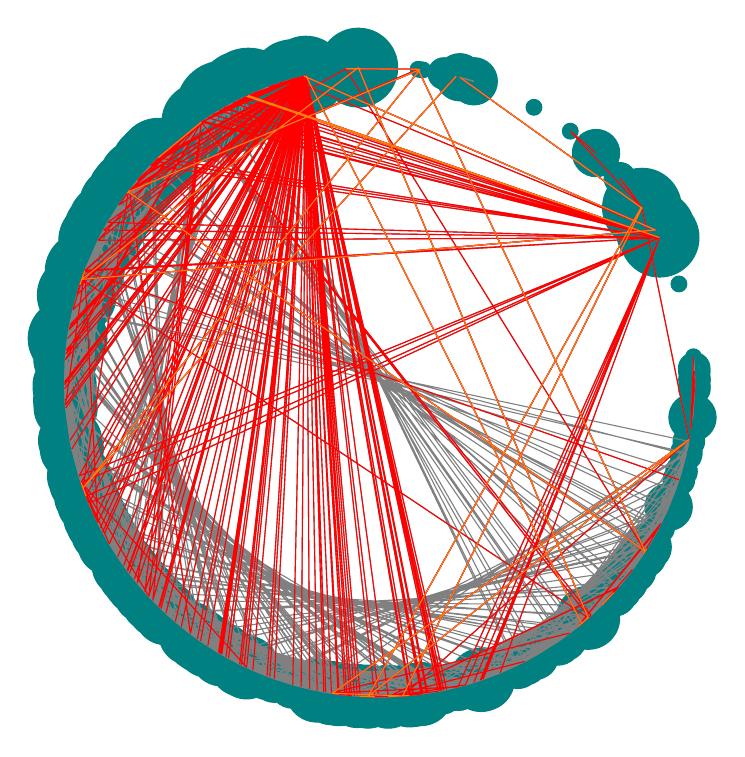
\begin{tikzpicture}
\filldraw[fill=teal, draw=teal]
(-4.0,-7.347880794884119E-16) circle (0.30000000000000004)(-0.01227182705186293,-3.9999811752383048) circle (0.30000000000000004)(3.9995293898168502,-0.061356825139952394) circle (0.2)(-0.06135682513995126,-3.9995293898168502) circle (0.30000000000000004)(3.999077621404861,-0.08589632110187793) circle (0.2)(-0.14722889176543433,-3.997289538353398) circle (0.4)(-0.24528294520883298,-3.9924724516005967) circle (0.30000000000000004)(-3.990045824561214,0.282018293558456) circle (0.4)(-0.2820182935584544,-3.990045824561214) circle (0.4)(-0.3187297518857198,-3.987281197164663) circle (0.30000000000000004)(-3.9841788036050083,0.355414210330096) circle (0.4)(-0.355414210330098,-3.984178803605008) circle (0.30000000000000004)(-0.37985398131855463,-3.9819230219677078) circle (0.30000000000000004)(-3.9795173231792225,0.4042794510193105) circle (0.4)(3.9795173231792225,-0.404279451019311) circle (0.2)(-0.4164865354882173,-3.978258282937022) circle (0.30000000000000004)(-0.440888829175532,-3.9756278800094242) circle (0.30000000000000004)(3.974256542082381,-0.45308380871025694) circle (0.30000000000000004)(3.9714016578394604,-0.4774608592439649) circle (0.1)(0.4896427007968648,3.96991813839484) circle (0.1)(-0.5139924431751713,-3.966839014676398) circle (0.4)(0.5139924431751727,3.966839014676398) circle (0.1)(-0.5261601148115324,-3.9652434393844618) circle (0.4)(-3.961940337025828,0.5504804863459447) circle (0.5)(0.5504804863459442,3.9619403370258284) circle (0.1)(-0.5990581387092848,-3.954886767841295) circle (0.2)(3.953030270922998,-0.6111887410337732) circle (0.1)(-0.6111887410337737,-3.953030270922998) circle (0.4)(-3.945232388978395,0.6596524819598776) circle (0.4)(-0.6838475550412039,-3.9411105695557653) circle (0.30000000000000004)(-3.941110569555765,0.6838475550412053) circle (0.4)(-0.7080168816485948,-3.9368403695477165) circle (0.30000000000000004)(-3.934649676846921,0.7200916056227988) circle (0.4)(3.932421949724865,-0.7321595518205637) circle (0.1)(3.927855476438221,-0.7562746565992247) circle (0.2)(3.9207285438724697,-0.7923936428718145) circle (0.1)(-0.7923936428718142,-3.9207285438724697) circle (0.4)(0.8164358643712675,3.915792701276249) circle (0.2)(3.9028085201541143,-0.8764049606274786) circle (0.1)(-0.8883744838928137,-3.9001013802679765) circle (0.30000000000000004)(3.8973575311423034,-0.9003356454391707) circle (0.2)(-3.894576998603248,0.912288332683543) circle (0.4)(3.8917598088222407,-0.9242324331226845) circle (0.2)(0.9719207196130555,3.880125012778176) circle (0.2)(-0.9957104229828795,-3.8740883770976695) circle (0.30000000000000004)(1.0194626384180583,3.8679058841794083) circle (0.30000000000000004)(-1.1022872772438324,-3.8451219432452826) circle (0.30000000000000004)(-3.8451219432452826,1.1022872772438321) circle (0.5)(3.8348138995834864,-1.1376301488450868) circle (0.2)(1.196319305232162,3.8169123804364227) circle (0.30000000000000004)(-3.813224161416775,1.2080237972769126) circle (0.4)(-3.805740083876034,1.231398560166139) circle (0.4)(3.8019442957979273,-1.2430686109984455) circle (0.2)(-3.782429301522085,1.3012411686490517) circle (0.4)(-1.3359986057680364,-3.770292790405788) circle (0.30000000000000004)(3.7536141362524327,-1.3821652998559562) circle (0.1)(-1.3936747209977383,-3.7493560476503) circle (0.2)(-3.745062668681114,1.4051710243422662) circle (0.5)(-3.740734039755791,1.4166541016819603) circle (0.4)(-1.4281238449337204,-3.7363702016170355) circle (0.30000000000000004)(3.671603102485562,-1.5872399496668412) circle (0.30000000000000004)(-1.6097386034376733,-3.6617948643530713) circle (0.30000000000000004)(3.6468241280217195,-1.6433726842316152) circle (0.2)(-1.6880010831991985,-3.626382818059662) circle (0.4)(-1.7213059253603307,-3.6106932729490353) circle (0.30000000000000004)(-1.7544649541541093,-3.594697862775816) circle (0.4)(-1.7764885782817164,-3.583864999024741) circle (0.2)(-3.5728972047820613,1.7984453186184264) circle (0.5)(3.572897204782061,-1.7984453186184268) circle (0.1)(3.5448901205955226,-1.8530391342074406) circle (0.2)(3.52768505739342,-1.8855869473039908) circle (0.1)(-1.9179750306406123,-3.510181160829045) circle (0.2)(-3.5042803767816277,1.9287350883164889) circle (0.5)(-1.9502006405937427,-3.492379913673161) circle (0.30000000000000004)(1.9609059331531646,3.486380346623804) circle (0.1)(3.4620544963622764,-2.0035415304449633) circle (0.2)(-2.003541530444963,-3.4620544963622764) circle (0.4)(-2.01415353490287,-3.4558914244863472) circle (0.2)(-2.02474658138062,-3.449695824444163) circle (0.2)(-3.449695824444163,2.02474658138062) circle (0.5)(-2.0353205701724284,-3.4434677545510692) circle (0.30000000000000004)(-2.045875401751881,-3.437207273428034) circle (0.30000000000000004)(3.405420772421061,-2.098358730713875) circle (0.30000000000000004)(3.392481379213189,-2.119214498745179) circle (0.1)(3.3728329585673813,-2.1503483051825825) circle (0.1)(-2.1812999536881845,-3.3528988222193528) circle (0.4)(3.346190908894048,-2.1915762366924008) circle (0.30000000000000004)(-3.3121801810310227,2.242646304789345) circle (0.5)(-2.273035810680526,-3.2913991255033057) circle (0.4)(-2.313255185646622,-3.2632576432269356) circle (0.4)(3.2128301259225798,-2.3827972179697334) circle (0.30000000000000004)(-3.2055046868925614,2.392642827985368) circle (0.5)(-2.4024659175354746,-3.198149076431621) circle (0.4)(-3.1907633637735655,2.4122663941613913) circle (0.1)(2.422044165617302,3.1833476184355343) circle (0.1)(-3.1759019102173482,2.431799139871095) circle (0.5)(-2.518552955659708,-3.1075538626929298) circle (0.30000000000000004)(3.1075538626929298,-2.5185529556597084) circle (0.30000000000000004)(-3.076413350582319,2.5564977794551025) circle (0.4)(-3.0606690624898367,2.5753261715591647) circle (0.5)(-3.052753669053525,2.584704051933265) circle (0.4)(-2.5940576040884493,-3.0448095419370476) circle (0.30000000000000004)(3.0368367559135523,-2.603386739985523) circle (0.2)(3.0288353860259387,-2.612691371815106) circle (0.30000000000000004)(2.9720318085404873,-2.6771303533865436) circle (0.30000000000000004)(2.94726627550948,-2.7043708143012632) circle (0.1)(-2.713400172519445,-2.938955512383855) circle (0.4)(2.749261363567036,2.905436620337384) circle (0.30000000000000004)(-2.905436620337385,2.749261363567035) circle (0.5)(-2.775885843558615,-2.8800100318455275) circle (0.30000000000000004)(-2.793504997635891,-2.862923301135275) circle (0.30000000000000004)(-2.802275175772993,-2.854339475123175) circle (0.4)(-2.854339475123175,2.8022751757729925) circle (0.5)(2.81973632150362,-2.837091305755462) circle (0.2)(-2.8110189778289025,2.8457287829808644) circle (0.5)(-2.8800100318455266,-2.775885843558616) circle (0.4)(-2.930617086689651,-2.722403991181813) circle (0.30000000000000004)(2.686235819388074,-2.9638045014198355) circle (0.2)(-2.9802311417658633,-2.6679996892145503) circle (0.4)(2.65884391281338,-2.98840242392072) circle (0.30000000000000004)(2.649663110360688,-2.9965455780938366) circle (0.4)(3.052753669053525,2.5847040519332656) circle (0.2)(3.060669062489836,2.575326171559166) circle (0.1)(2.5659240512343326,-3.068555647743281) circle (0.1)(-3.076413350582318,-2.556497779455104) circle (0.4)(-2.547047444945137,3.0842420970472553) circle (0.1)(2.518552955659709,-3.1075538626929293) circle (0.30000000000000004)(-3.1152660495259026,-2.5090072619805777) circle (0.4)(2.4802288470531577,-3.1382263886223) circle (0.2)(-3.1759019102173474,-2.4317991398710963) circle (0.4)(2.4122663941613935,-3.1907633637735637) circle (0.2)(3.19814907643162,2.402465917535476) circle (0.30000000000000004)(-3.198149076431619,-2.4024659175354772) circle (0.30000000000000004)(-3.2055046868925605,-2.3926428279853695) circle (0.30000000000000004)(2.333234611750794,-3.249002346340815) circle (0.30000000000000004)(-3.249002346340816,-2.333234611750793) circle (0.4)(2.313255185646623,-3.263257643226935) circle (0.2)(-2.2629272431344543,3.2983572111401003) circle (0.5)(2.262927243134454,-3.2983572111401003) circle (0.30000000000000004)(-2.2426463047893463,3.3121801810310214) circle (0.5)(3.325878449210181,2.222280932078409) circle (0.1)(-3.325878449210181,-2.2222809320784087) circle (0.2)(3.3326806588076527,2.2120668223201103) circle (0.5)(3.33945149994552,2.2018318917464192) circle (0.2)(-2.181299953688187,3.352898822219351) circle (0.4)(-2.1192144987451798,3.3924813792131885) circle (0.5)(-3.430914440001088,-2.056410976772887) circle (0.4)(-2.0353205701724297,3.4434677545510683) circle (0.4)(2.024746581380621,-3.449695824444162) circle (0.2)(-1.9822610473030922,3.4742828238853627) circle (0.6000000000000001)(1.9715927689191366,-3.4803479644348454) circle (0.30000000000000004)(-1.971592768919137,3.4803479644348454) circle (0.4)(-3.4983466091127045,-1.9394769920031647) circle (0.30000000000000004)(3.5042803767816264,1.9287350883164913) circle (0.5)(-3.5160489057145337,-1.9071969202532886) circle (0.4)(-1.8639059830718667,3.53918839372375) circle (0.5)(-3.544890120595522,-1.8530391342074415) circle (0.30000000000000004)(1.842154843832961,-3.5505584816114153) circle (0.30000000000000004)(3.5561934234186583,1.8312532143955091) circle (0.5)(-1.798445318618428,3.5728972047820604) circle (0.5)(-3.578397942525531,-1.7874753606494969) circle (0.4)(1.7544649541541102,-3.5946978627758157) circle (0.30000000000000004)(1.7323752754126083,-3.6053953881840877) circle (0.2)(-1.732375275412609,3.6053953881840877) circle (0.6000000000000001)(-3.6106932729490353,-1.72130592536033) circle (0.4)(-1.6880010831991983,3.626382818059662) circle (0.5)(-1.665718240390549,3.6366719323620895) circle (0.6000000000000001)(-1.6545532489537407,3.6417651690322677) circle (0.30000000000000004)(-1.5872399496668432,3.671603102485561) circle (0.2)(-3.690804513335514,-1.5420642153756756) circle (0.4)(1.5307337294603596,-3.695518130045147) circle (0.2)(-3.727537062326672,-1.4510228974695893) circle (0.4)(-1.4051710243422677,3.7450626686811135) circle (0.2)(-1.3706428692479797,3.757836894408759) circle (0.30000000000000004)(-1.3591075376273085,3.7620242823730727) circle (0.4)(-3.7661762607320832,-1.3475594135688798) circle (0.1)(1.3128393743163709,-3.7784193490459206) circle (0.4)(1.2896307152042794,-3.786403652333134) circle (0.4)(-3.790342364070965,-1.2780081232640617) circle (0.4)(1.2780081232640632,-3.7903423640709644) circle (0.1)(-1.266373502224665,3.7942453996629206) circle (0.4)(3.801944295797927,1.243068610998446) circle (0.1)(1.1963193052321621,-3.8169123804364222) circle (0.30000000000000004)(-3.8169123804364222,-1.1963193052321623) circle (0.4)(-1.1493898381789174,3.8313056521101316) circle (0.4)(-1.1258597517030322,3.838286052327938) circle (0.5)(-1.1022872772438337,3.845121943245282) circle (0.5)(1.090485421799797,-3.848485617076166) circle (0.30000000000000004)(-1.0786733022916624,3.851813067494735) circle (0.4)(0.9957104229828804,-3.8740883770976695) circle (0.30000000000000004)(-0.9600120897949658,3.8830885629158014) circle (0.4)(-0.9361678343341745,3.888905988315745) circle (0.5)(0.8524412796643657,-3.908112570631017) circle (0.2)(-3.908112570631017,-0.8524412796643677) circle (0.4)(0.8164358643712674,-3.915792701276249) circle (0.2)(0.7923936428718152,-3.9207285438724693) circle (0.2)(0.7803612880645144,-3.9231411216129217) circle (0.30000000000000004)(0.7683215881995699,-3.9255167732550182) circle (0.2)(0.7442206066537876,-3.930157209149765) circle (0.2)(-3.930157209149765,-0.7442206066537879) circle (0.4)(0.6111887410337747,-3.953030270922998) circle (0.30000000000000004)(0.5990581387092858,-3.954886767841295) circle (0.2)(0.5504804863459442,-3.9619403370258284) circle (0.2)(0.5383228340285051,-3.96361054171112) circle (0.2)(0.5261601148115334,-3.9652434393844613) circle (0.4)(0.42868969982723665,-3.9769617978127516) circle (0.4)(-0.42868969982723537,3.9769617978127516) circle (0.1)(0.3920685613182433,-3.9807389066887873) circle (0.4)(0.37985398131855563,-3.9819230219677078) circle (0.4)(-3.9862845831622193,-0.3309610581975028) circle (0.4)(3.9872811971646627,0.3187297518857205) circle (0.1)(-3.989161826714761,-0.2942582543986694) circle (0.4)(0.2942582543986709,-3.989161826714761) circle (0.2)(-0.26977567825465715,3.9908922665767665) circle (0.5)(-3.993206179735571,-0.23303305800174343) circle (0.4)(3.9963109110105814,0.17175302773976384) circle (0.2)(3.997722418221847,0.13496468740551057) circle (0.2)(0.11043258311586264,-3.9984752899807146) circle (0.4)(-3.999077621404861,-0.08589632110187714) circle (0.4)(-3.9998305782078556,-0.03681501912824033) circle (0.4)(3.9998305782078556,0.03681501912823984) circle (0.2)(3.9999247011304044,0.02454353859661806) circle (0.2)(-3.9999247011304044,-0.024543538596617665) circle (0.30000000000000004);
\draw [gray]
(-4.0,-7.347880794884119E-16) -- (-3.990045824561214,0.282018293558456)
(-4.0,-7.347880794884119E-16) -- (-3.990045824561214,0.282018293558456)
(-4.0,-7.347880794884119E-16) -- (-3.990045824561214,0.282018293558456)
(-4.0,-7.347880794884119E-16) -- (-3.990045824561214,0.282018293558456)
(-4.0,-7.347880794884119E-16) -- (-3.990045824561214,0.282018293558456)
(-4.0,-7.347880794884119E-16) -- (-3.9795173231792225,0.4042794510193105)
(-4.0,-7.347880794884119E-16) -- (-3.894576998603248,0.912288332683543)
(-4.0,-7.347880794884119E-16) -- (-3.5728972047820613,1.7984453186184264)
(-4.0,-7.347880794884119E-16) -- (-2.8110189778289025,2.8457287829808644)
(-4.0,-7.347880794884119E-16) -- (-0.9361678343341745,3.888905988315745)
(-4.0,-7.347880794884119E-16) -- (-0.9361678343341745,3.888905988315745)
(-0.01227182705186293,-3.9999811752383048) -- (-0.06135682513995126,-3.9995293898168502)
(-0.01227182705186293,-3.9999811752383048) -- (-0.06135682513995126,-3.9995293898168502)
(-0.01227182705186293,-3.9999811752383048) -- (-0.06135682513995126,-3.9995293898168502)
(-0.01227182705186293,-3.9999811752383048) -- (-0.24528294520883298,-3.9924724516005967)
(-0.01227182705186293,-3.9999811752383048) -- (-0.24528294520883298,-3.9924724516005967)
(-0.01227182705186293,-3.9999811752383048) -- (-0.4164865354882173,-3.978258282937022)
(-0.01227182705186293,-3.9999811752383048) -- (-0.7923936428718142,-3.9207285438724697)
(-0.01227182705186293,-3.9999811752383048) -- (-1.6097386034376733,-3.6617948643530713)
(-0.01227182705186293,-3.9999811752383048) -- (-2.8800100318455266,-2.775885843558616)
(-0.01227182705186293,-3.9999811752383048) -- (-3.990045824561214,0.282018293558456)
(-0.01227182705186293,-3.9999811752383048) -- (-0.9361678343341745,3.888905988315745)
(3.9995293898168502,-0.061356825139952394) -- (3.999077621404861,-0.08589632110187793)
(3.9995293898168502,-0.061356825139952394) -- (3.999077621404861,-0.08589632110187793)
(3.9995293898168502,-0.061356825139952394) -- (3.9795173231792225,-0.404279451019311)
(3.9995293898168502,-0.061356825139952394) -- (3.9795173231792225,-0.404279451019311)
(3.9995293898168502,-0.061356825139952394) -- (3.9795173231792225,-0.404279451019311)
(3.9995293898168502,-0.061356825139952394) -- (3.974256542082381,-0.45308380871025694)
(3.9995293898168502,-0.061356825139952394) -- (3.953030270922998,-0.6111887410337732)
(3.9995293898168502,-0.061356825139952394) -- (3.953030270922998,-0.6111887410337732)
(3.9995293898168502,-0.061356825139952394) -- (3.953030270922998,-0.6111887410337732)
(3.9995293898168502,-0.061356825139952394) -- (3.953030270922998,-0.6111887410337732)
(3.9995293898168502,-0.061356825139952394) -- (3.953030270922998,-0.6111887410337732)
(-0.06135682513995126,-3.9995293898168502) -- (-0.24528294520883298,-3.9924724516005967)
(-0.06135682513995126,-3.9995293898168502) -- (-0.24528294520883298,-3.9924724516005967)
(-0.06135682513995126,-3.9995293898168502) -- (-0.24528294520883298,-3.9924724516005967)
(-0.06135682513995126,-3.9995293898168502) -- (-0.24528294520883298,-3.9924724516005967)
(-0.06135682513995126,-3.9995293898168502) -- (-0.2820182935584544,-3.990045824561214)
(-0.06135682513995126,-3.9995293898168502) -- (-0.5139924431751713,-3.966839014676398)
(-0.06135682513995126,-3.9995293898168502) -- (-0.8883744838928137,-3.9001013802679765)
(-0.06135682513995126,-3.9995293898168502) -- (-1.6097386034376733,-3.6617948643530713)
(-0.06135682513995126,-3.9995293898168502) -- (-2.8800100318455266,-2.775885843558616)
(-0.06135682513995126,-3.9995293898168502) -- (-3.990045824561214,0.282018293558456)
(-0.06135682513995126,-3.9995293898168502) -- (-0.9361678343341745,3.888905988315745)
(3.999077621404861,-0.08589632110187793) -- (3.9795173231792225,-0.404279451019311)
(3.999077621404861,-0.08589632110187793) -- (3.9795173231792225,-0.404279451019311)
(3.999077621404861,-0.08589632110187793) -- (3.9795173231792225,-0.404279451019311)
(3.999077621404861,-0.08589632110187793) -- (3.9795173231792225,-0.404279451019311)
(3.999077621404861,-0.08589632110187793) -- (3.9795173231792225,-0.404279451019311)
(3.999077621404861,-0.08589632110187793) -- (3.9714016578394604,-0.4774608592439649)
(3.999077621404861,-0.08589632110187793) -- (3.953030270922998,-0.6111887410337732)
(3.999077621404861,-0.08589632110187793) -- (3.953030270922998,-0.6111887410337732)
(3.999077621404861,-0.08589632110187793) -- (3.953030270922998,-0.6111887410337732)
(3.999077621404861,-0.08589632110187793) -- (3.953030270922998,-0.6111887410337732)
(3.999077621404861,-0.08589632110187793) -- (3.953030270922998,-0.6111887410337732)
(-0.14722889176543433,-3.997289538353398) -- (3.932421949724865,-0.7321595518205637)
(-0.14722889176543433,-3.997289538353398) -- (3.932421949724865,-0.7321595518205637)
(-0.14722889176543433,-3.997289538353398) -- (3.932421949724865,-0.7321595518205637)
(-0.14722889176543433,-3.997289538353398) -- (3.932421949724865,-0.7321595518205637)
(-0.14722889176543433,-3.997289538353398) -- (3.932421949724865,-0.7321595518205637)
(-0.14722889176543433,-3.997289538353398) -- (3.932421949724865,-0.7321595518205637)
(-0.14722889176543433,-3.997289538353398) -- (3.932421949724865,-0.7321595518205637)
(-0.14722889176543433,-3.997289538353398) -- (3.932421949724865,-0.7321595518205637)
(-0.14722889176543433,-3.997289538353398) -- (3.932421949724865,-0.7321595518205637)
(-0.14722889176543433,-3.997289538353398) -- (3.932421949724865,-0.7321595518205637)
(-0.14722889176543433,-3.997289538353398) -- (3.932421949724865,-0.7321595518205637)
(-0.24528294520883298,-3.9924724516005967) -- (-0.2820182935584544,-3.990045824561214)
(-0.24528294520883298,-3.9924724516005967) -- (-0.2820182935584544,-3.990045824561214)
(-0.24528294520883298,-3.9924724516005967) -- (-0.3187297518857198,-3.987281197164663)
(-0.24528294520883298,-3.9924724516005967) -- (-0.355414210330098,-3.984178803605008)
(-0.24528294520883298,-3.9924724516005967) -- (-0.440888829175532,-3.9756278800094242)
(-0.24528294520883298,-3.9924724516005967) -- (-0.6838475550412039,-3.9411105695557653)
(-0.24528294520883298,-3.9924724516005967) -- (-1.1022872772438324,-3.8451219432452826)
(-0.24528294520883298,-3.9924724516005967) -- (-1.7544649541541093,-3.594697862775816)
(-0.24528294520883298,-3.9924724516005967) -- (-3.076413350582318,-2.556497779455104)
(-0.24528294520883298,-3.9924724516005967) -- (-3.990045824561214,0.282018293558456)
(-0.24528294520883298,-3.9924724516005967) -- (-0.9361678343341745,3.888905988315745)
(-3.990045824561214,0.282018293558456) -- (-3.9841788036050083,0.355414210330096)
(-3.990045824561214,0.282018293558456) -- (-3.9841788036050083,0.355414210330096)
(-3.990045824561214,0.282018293558456) -- (-3.9841788036050083,0.355414210330096)
(-3.990045824561214,0.282018293558456) -- (-3.9795173231792225,0.4042794510193105)
(-3.990045824561214,0.282018293558456) -- (-3.961940337025828,0.5504804863459447)
(-3.990045824561214,0.282018293558456) -- (-3.941110569555765,0.6838475550412053)
(-3.990045824561214,0.282018293558456) -- (-3.8451219432452826,1.1022872772438321)
(-3.990045824561214,0.282018293558456) -- (-3.5728972047820613,1.7984453186184264)
(-3.990045824561214,0.282018293558456) -- (-2.2629272431344543,3.2983572111401003)
(-3.990045824561214,0.282018293558456) -- (-0.9361678343341745,3.888905988315745)
(-3.990045824561214,0.282018293558456) -- (-0.9361678343341745,3.888905988315745)
(-0.2820182935584544,-3.990045824561214) -- (-0.3187297518857198,-3.987281197164663)
(-0.2820182935584544,-3.990045824561214) -- (-0.3187297518857198,-3.987281197164663)
(-0.2820182935584544,-3.990045824561214) -- (-0.355414210330098,-3.984178803605008)
(-0.2820182935584544,-3.990045824561214) -- (-0.37985398131855463,-3.9819230219677078)
(-0.2820182935584544,-3.990045824561214) -- (-0.5139924431751713,-3.966839014676398)
(-0.2820182935584544,-3.990045824561214) -- (-0.6838475550412039,-3.9411105695557653)
(-0.2820182935584544,-3.990045824561214) -- (-1.1022872772438324,-3.8451219432452826)
(-0.2820182935584544,-3.990045824561214) -- (-1.9179750306406123,-3.510181160829045)
(-0.2820182935584544,-3.990045824561214) -- (-3.076413350582318,-2.556497779455104)
(-0.2820182935584544,-3.990045824561214) -- (-3.990045824561214,0.282018293558456)
(-0.2820182935584544,-3.990045824561214) -- (-0.9361678343341745,3.888905988315745)
(-0.3187297518857198,-3.987281197164663) -- (-0.355414210330098,-3.984178803605008)
(-0.3187297518857198,-3.987281197164663) -- (-0.355414210330098,-3.984178803605008)
(-0.3187297518857198,-3.987281197164663) -- (-0.37985398131855463,-3.9819230219677078)
(-0.3187297518857198,-3.987281197164663) -- (-0.4164865354882173,-3.978258282937022)
(-0.3187297518857198,-3.987281197164663) -- (-0.5139924431751713,-3.966839014676398)
(-0.3187297518857198,-3.987281197164663) -- (-0.7080168816485948,-3.9368403695477165)
(-0.3187297518857198,-3.987281197164663) -- (-1.1022872772438324,-3.8451219432452826)
(-0.3187297518857198,-3.987281197164663) -- (-1.9179750306406123,-3.510181160829045)
(-0.3187297518857198,-3.987281197164663) -- (-3.076413350582318,-2.556497779455104)
(-0.3187297518857198,-3.987281197164663) -- (-3.9841788036050083,0.355414210330096)
(-0.3187297518857198,-3.987281197164663) -- (-0.9361678343341745,3.888905988315745)
(-3.9841788036050083,0.355414210330096) -- (-3.9795173231792225,0.4042794510193105)
(-3.9841788036050083,0.355414210330096) -- (-3.9795173231792225,0.4042794510193105)
(-3.9841788036050083,0.355414210330096) -- (-3.9795173231792225,0.4042794510193105)
(-3.9841788036050083,0.355414210330096) -- (-3.961940337025828,0.5504804863459447)
(-3.9841788036050083,0.355414210330096) -- (-3.961940337025828,0.5504804863459447)
(-3.9841788036050083,0.355414210330096) -- (-3.894576998603248,0.912288332683543)
(-3.9841788036050083,0.355414210330096) -- (-3.813224161416775,1.2080237972769126)
(-3.9841788036050083,0.355414210330096) -- (-3.5042803767816277,1.9287350883164889)
(-3.9841788036050083,0.355414210330096) -- (-2.2629272431344543,3.2983572111401003)
(-3.9841788036050083,0.355414210330096) -- (-0.9361678343341745,3.888905988315745)
(-3.9841788036050083,0.355414210330096) -- (-0.9361678343341745,3.888905988315745)
(-0.355414210330098,-3.984178803605008) -- (-0.37985398131855463,-3.9819230219677078)
(-0.355414210330098,-3.984178803605008) -- (-0.37985398131855463,-3.9819230219677078)
(-0.355414210330098,-3.984178803605008) -- (-0.4164865354882173,-3.978258282937022)
(-0.355414210330098,-3.984178803605008) -- (-0.5139924431751713,-3.966839014676398)
(-0.355414210330098,-3.984178803605008) -- (-0.6111887410337737,-3.953030270922998)
(-0.355414210330098,-3.984178803605008) -- (-0.7923936428718142,-3.9207285438724697)
(-0.355414210330098,-3.984178803605008) -- (-1.3359986057680364,-3.770292790405788)
(-0.355414210330098,-3.984178803605008) -- (-1.9179750306406123,-3.510181160829045)
(-0.355414210330098,-3.984178803605008) -- (-3.076413350582318,-2.556497779455104)
(-0.355414210330098,-3.984178803605008) -- (-3.9841788036050083,0.355414210330096)
(-0.355414210330098,-3.984178803605008) -- (-0.9361678343341745,3.888905988315745)
(-0.37985398131855463,-3.9819230219677078) -- (-0.4164865354882173,-3.978258282937022)
(-0.37985398131855463,-3.9819230219677078) -- (-0.4164865354882173,-3.978258282937022)
(-0.37985398131855463,-3.9819230219677078) -- (-0.440888829175532,-3.9756278800094242)
(-0.37985398131855463,-3.9819230219677078) -- (-0.5139924431751713,-3.966839014676398)
(-0.37985398131855463,-3.9819230219677078) -- (-0.6111887410337737,-3.953030270922998)
(-0.37985398131855463,-3.9819230219677078) -- (-0.7923936428718142,-3.9207285438724697)
(-0.37985398131855463,-3.9819230219677078) -- (-1.3359986057680364,-3.770292790405788)
(-0.37985398131855463,-3.9819230219677078) -- (-1.9179750306406123,-3.510181160829045)
(-0.37985398131855463,-3.9819230219677078) -- (-3.1152660495259026,-2.5090072619805777)
(-0.37985398131855463,-3.9819230219677078) -- (-3.9795173231792225,0.4042794510193105)
(-0.37985398131855463,-3.9819230219677078) -- (-0.9361678343341745,3.888905988315745)
(-3.9795173231792225,0.4042794510193105) -- (-3.961940337025828,0.5504804863459447)
(-3.9795173231792225,0.4042794510193105) -- (-3.961940337025828,0.5504804863459447)
(-3.9795173231792225,0.4042794510193105) -- (-3.961940337025828,0.5504804863459447)
(-3.9795173231792225,0.4042794510193105) -- (-3.961940337025828,0.5504804863459447)
(-3.9795173231792225,0.4042794510193105) -- (-3.945232388978395,0.6596524819598776)
(-3.9795173231792225,0.4042794510193105) -- (-3.894576998603248,0.912288332683543)
(-3.9795173231792225,0.4042794510193105) -- (-3.813224161416775,1.2080237972769126)
(-3.9795173231792225,0.4042794510193105) -- (-3.5042803767816277,1.9287350883164889)
(-3.9795173231792225,0.4042794510193105) -- (-2.2629272431344543,3.2983572111401003)
(-3.9795173231792225,0.4042794510193105) -- (-0.9361678343341745,3.888905988315745)
(-3.9795173231792225,0.4042794510193105) -- (-0.9361678343341745,3.888905988315745)
(3.9795173231792225,-0.404279451019311) -- (3.974256542082381,-0.45308380871025694)
(3.9795173231792225,-0.404279451019311) -- (3.974256542082381,-0.45308380871025694)
(3.9795173231792225,-0.404279451019311) -- (3.974256542082381,-0.45308380871025694)
(-0.4164865354882173,-3.978258282937022) -- (-0.440888829175532,-3.9756278800094242)
(-0.4164865354882173,-3.978258282937022) -- (-0.440888829175532,-3.9756278800094242)
(-0.4164865354882173,-3.978258282937022) -- (-0.5139924431751713,-3.966839014676398)
(-0.4164865354882173,-3.978258282937022) -- (-0.5139924431751713,-3.966839014676398)
(-0.4164865354882173,-3.978258282937022) -- (-0.6111887410337737,-3.953030270922998)
(-0.4164865354882173,-3.978258282937022) -- (-0.8883744838928137,-3.9001013802679765)
(-0.4164865354882173,-3.978258282937022) -- (-1.3359986057680364,-3.770292790405788)
(-0.4164865354882173,-3.978258282937022) -- (-1.9179750306406123,-3.510181160829045)
(-0.4164865354882173,-3.978258282937022) -- (-3.1152660495259026,-2.5090072619805777)
(-0.4164865354882173,-3.978258282937022) -- (-3.961940337025828,0.5504804863459447)
(-0.4164865354882173,-3.978258282937022) -- (-0.9361678343341745,3.888905988315745)
(-0.440888829175532,-3.9756278800094242) -- (-0.5139924431751713,-3.966839014676398)
(-0.440888829175532,-3.9756278800094242) -- (-0.5139924431751713,-3.966839014676398)
(-0.440888829175532,-3.9756278800094242) -- (-0.5139924431751713,-3.966839014676398)
(-0.440888829175532,-3.9756278800094242) -- (-0.6111887410337737,-3.953030270922998)
(-0.440888829175532,-3.9756278800094242) -- (-0.6838475550412039,-3.9411105695557653)
(-0.440888829175532,-3.9756278800094242) -- (-0.8883744838928137,-3.9001013802679765)
(-0.440888829175532,-3.9756278800094242) -- (-1.3359986057680364,-3.770292790405788)
(-0.440888829175532,-3.9756278800094242) -- (-1.9502006405937427,-3.492379913673161)
(-0.440888829175532,-3.9756278800094242) -- (-3.1759019102173474,-2.4317991398710963)
(-0.440888829175532,-3.9756278800094242) -- (-3.961940337025828,0.5504804863459447)
(-0.440888829175532,-3.9756278800094242) -- (-0.9361678343341745,3.888905988315745)
(3.974256542082381,-0.45308380871025694) -- (3.9714016578394604,-0.4774608592439649)
(3.974256542082381,-0.45308380871025694) -- (3.9714016578394604,-0.4774608592439649)
(0.4896427007968648,3.96991813839484) -- (3.3728329585673813,-2.1503483051825825)
(0.4896427007968648,3.96991813839484) -- (3.3728329585673813,-2.1503483051825825)
(0.4896427007968648,3.96991813839484) -- (3.3728329585673813,-2.1503483051825825)
(0.4896427007968648,3.96991813839484) -- (3.3728329585673813,-2.1503483051825825)
(0.4896427007968648,3.96991813839484) -- (3.3728329585673813,-2.1503483051825825)
(0.4896427007968648,3.96991813839484) -- (3.3728329585673813,-2.1503483051825825)
(0.4896427007968648,3.96991813839484) -- (3.3728329585673813,-2.1503483051825825)
(0.4896427007968648,3.96991813839484) -- (3.3728329585673813,-2.1503483051825825)
(0.4896427007968648,3.96991813839484) -- (3.3728329585673813,-2.1503483051825825)
(0.4896427007968648,3.96991813839484) -- (3.3728329585673813,-2.1503483051825825)
(0.4896427007968648,3.96991813839484) -- (-3.1907633637735655,2.4122663941613913)
(-0.5139924431751713,-3.966839014676398) -- (-0.5261601148115324,-3.9652434393844618)
(-0.5139924431751713,-3.966839014676398) -- (-0.6111887410337737,-3.953030270922998)
(-0.5139924431751713,-3.966839014676398) -- (-0.6111887410337737,-3.953030270922998)
(-0.5139924431751713,-3.966839014676398) -- (-0.6111887410337737,-3.953030270922998)
(-0.5139924431751713,-3.966839014676398) -- (-0.7080168816485948,-3.9368403695477165)
(-0.5139924431751713,-3.966839014676398) -- (-0.9957104229828795,-3.8740883770976695)
(-0.5139924431751713,-3.966839014676398) -- (-1.3359986057680364,-3.770292790405788)
(-0.5139924431751713,-3.966839014676398) -- (-2.003541530444963,-3.4620544963622764)
(-0.5139924431751713,-3.966839014676398) -- (-3.1759019102173474,-2.4317991398710963)
(-0.5139924431751713,-3.966839014676398) -- (-3.961940337025828,0.5504804863459447)
(-0.5139924431751713,-3.966839014676398) -- (-0.9361678343341745,3.888905988315745)
(0.5139924431751727,3.966839014676398) -- (-3.7661762607320832,-1.3475594135688798)
(0.5139924431751727,3.966839014676398) -- (-3.7661762607320832,-1.3475594135688798)
(0.5139924431751727,3.966839014676398) -- (-3.7661762607320832,-1.3475594135688798)
(0.5139924431751727,3.966839014676398) -- (-3.7661762607320832,-1.3475594135688798)
(0.5139924431751727,3.966839014676398) -- (-3.7661762607320832,-1.3475594135688798)
(0.5139924431751727,3.966839014676398) -- (-3.7661762607320832,-1.3475594135688798)
(0.5139924431751727,3.966839014676398) -- (-3.7661762607320832,-1.3475594135688798)
(0.5139924431751727,3.966839014676398) -- (-3.7661762607320832,-1.3475594135688798)
(0.5139924431751727,3.966839014676398) -- (-3.7661762607320832,-1.3475594135688798)
(0.5139924431751727,3.966839014676398) -- (-3.7661762607320832,-1.3475594135688798)
(0.5139924431751727,3.966839014676398) -- (-3.7661762607320832,-1.3475594135688798)
(-0.5261601148115324,-3.9652434393844618) -- (-0.6111887410337737,-3.953030270922998)
(-0.5261601148115324,-3.9652434393844618) -- (-0.6111887410337737,-3.953030270922998)
(-0.5261601148115324,-3.9652434393844618) -- (-0.6111887410337737,-3.953030270922998)
(-0.5261601148115324,-3.9652434393844618) -- (-0.6838475550412039,-3.9411105695557653)
(-0.5261601148115324,-3.9652434393844618) -- (-0.7923936428718142,-3.9207285438724697)
(-0.5261601148115324,-3.9652434393844618) -- (-0.9957104229828795,-3.8740883770976695)
(-0.5261601148115324,-3.9652434393844618) -- (-1.3359986057680364,-3.770292790405788)
(-0.5261601148115324,-3.9652434393844618) -- (-2.003541530444963,-3.4620544963622764)
(-0.5261601148115324,-3.9652434393844618) -- (-3.1759019102173474,-2.4317991398710963)
(-0.5261601148115324,-3.9652434393844618) -- (-3.961940337025828,0.5504804863459447)
(-0.5261601148115324,-3.9652434393844618) -- (-0.9361678343341745,3.888905988315745)
(-3.961940337025828,0.5504804863459447) -- (-3.945232388978395,0.6596524819598776)
(-3.961940337025828,0.5504804863459447) -- (-3.945232388978395,0.6596524819598776)
(-3.961940337025828,0.5504804863459447) -- (-3.945232388978395,0.6596524819598776)
(-3.961940337025828,0.5504804863459447) -- (-3.945232388978395,0.6596524819598776)
(-3.961940337025828,0.5504804863459447) -- (-3.894576998603248,0.912288332683543)
(-3.961940337025828,0.5504804863459447) -- (-3.8451219432452826,1.1022872772438321)
(-3.961940337025828,0.5504804863459447) -- (-3.745062668681114,1.4051710243422662)
(-3.961940337025828,0.5504804863459447) -- (-3.449695824444163,2.02474658138062)
(-3.961940337025828,0.5504804863459447) -- (-2.2629272431344543,3.2983572111401003)
(-3.961940337025828,0.5504804863459447) -- (-0.9361678343341745,3.888905988315745)
(-3.961940337025828,0.5504804863459447) -- (-0.9361678343341745,3.888905988315745)
(-0.5990581387092848,-3.954886767841295) -- (0.2942582543986709,-3.989161826714761)
(-0.5990581387092848,-3.954886767841295) -- (0.2942582543986709,-3.989161826714761)
(-0.5990581387092848,-3.954886767841295) -- (0.2942582543986709,-3.989161826714761)
(-0.5990581387092848,-3.954886767841295) -- (0.2942582543986709,-3.989161826714761)
(-0.5990581387092848,-3.954886767841295) -- (0.2942582543986709,-3.989161826714761)
(-0.5990581387092848,-3.954886767841295) -- (0.2942582543986709,-3.989161826714761)
(-0.5990581387092848,-3.954886767841295) -- (0.2942582543986709,-3.989161826714761)
(-0.5990581387092848,-3.954886767841295) -- (0.2942582543986709,-3.989161826714761)
(-0.5990581387092848,-3.954886767841295) -- (0.2942582543986709,-3.989161826714761)
(-0.5990581387092848,-3.954886767841295) -- (0.2942582543986709,-3.989161826714761)
(-0.5990581387092848,-3.954886767841295) -- (0.2942582543986709,-3.989161826714761)
(-0.6111887410337737,-3.953030270922998) -- (-0.6838475550412039,-3.9411105695557653)
(-0.6111887410337737,-3.953030270922998) -- (-0.6838475550412039,-3.9411105695557653)
(-0.6111887410337737,-3.953030270922998) -- (-0.6838475550412039,-3.9411105695557653)
(-0.6111887410337737,-3.953030270922998) -- (-0.7080168816485948,-3.9368403695477165)
(-0.6111887410337737,-3.953030270922998) -- (-0.8883744838928137,-3.9001013802679765)
(-0.6111887410337737,-3.953030270922998) -- (-0.9957104229828795,-3.8740883770976695)
(-0.6111887410337737,-3.953030270922998) -- (-1.3936747209977383,-3.7493560476503)
(-0.6111887410337737,-3.953030270922998) -- (-2.1812999536881845,-3.3528988222193528)
(-0.6111887410337737,-3.953030270922998) -- (-3.249002346340816,-2.333234611750793)
(-0.6111887410337737,-3.953030270922998) -- (-3.945232388978395,0.6596524819598776)
(-0.6111887410337737,-3.953030270922998) -- (-0.9361678343341745,3.888905988315745)
(-3.945232388978395,0.6596524819598776) -- (-3.941110569555765,0.6838475550412053)
(-3.945232388978395,0.6596524819598776) -- (-3.941110569555765,0.6838475550412053)
(-3.945232388978395,0.6596524819598776) -- (-3.934649676846921,0.7200916056227988)
(-3.945232388978395,0.6596524819598776) -- (-3.894576998603248,0.912288332683543)
(-3.945232388978395,0.6596524819598776) -- (-3.894576998603248,0.912288332683543)
(-3.945232388978395,0.6596524819598776) -- (-3.8451219432452826,1.1022872772438321)
(-3.945232388978395,0.6596524819598776) -- (-3.740734039755791,1.4166541016819603)
(-3.945232388978395,0.6596524819598776) -- (-3.3121801810310227,2.242646304789345)
(-3.945232388978395,0.6596524819598776) -- (-2.2629272431344543,3.2983572111401003)
(-3.945232388978395,0.6596524819598776) -- (-0.9361678343341745,3.888905988315745)
(-3.945232388978395,0.6596524819598776) -- (-0.9361678343341745,3.888905988315745)
(-0.6838475550412039,-3.9411105695557653) -- (-0.7080168816485948,-3.9368403695477165)
(-0.6838475550412039,-3.9411105695557653) -- (-0.7080168816485948,-3.9368403695477165)
(-0.6838475550412039,-3.9411105695557653) -- (-0.7923936428718142,-3.9207285438724697)
(-0.6838475550412039,-3.9411105695557653) -- (-0.7923936428718142,-3.9207285438724697)
(-0.6838475550412039,-3.9411105695557653) -- (-0.8883744838928137,-3.9001013802679765)
(-0.6838475550412039,-3.9411105695557653) -- (-1.1022872772438324,-3.8451219432452826)
(-0.6838475550412039,-3.9411105695557653) -- (-1.6097386034376733,-3.6617948643530713)
(-0.6838475550412039,-3.9411105695557653) -- (-2.1812999536881845,-3.3528988222193528)
(-0.6838475550412039,-3.9411105695557653) -- (-3.325878449210181,-2.2222809320784087)
(-0.6838475550412039,-3.9411105695557653) -- (-3.941110569555765,0.6838475550412053)
(-0.6838475550412039,-3.9411105695557653) -- (-0.9361678343341745,3.888905988315745)
(-3.941110569555765,0.6838475550412053) -- (-3.934649676846921,0.7200916056227988)
(-3.941110569555765,0.6838475550412053) -- (-3.934649676846921,0.7200916056227988)
(-3.941110569555765,0.6838475550412053) -- (-3.894576998603248,0.912288332683543)
(-3.941110569555765,0.6838475550412053) -- (-3.894576998603248,0.912288332683543)
(-3.941110569555765,0.6838475550412053) -- (-3.894576998603248,0.912288332683543)
(-3.941110569555765,0.6838475550412053) -- (-3.8451219432452826,1.1022872772438321)
(-3.941110569555765,0.6838475550412053) -- (-3.5728972047820613,1.7984453186184264)
(-3.941110569555765,0.6838475550412053) -- (-3.3121801810310227,2.242646304789345)
(-3.941110569555765,0.6838475550412053) -- (-2.2629272431344543,3.2983572111401003)
(-3.941110569555765,0.6838475550412053) -- (-0.9361678343341745,3.888905988315745)
(-3.941110569555765,0.6838475550412053) -- (-0.9361678343341745,3.888905988315745)
(-0.7080168816485948,-3.9368403695477165) -- (-0.7923936428718142,-3.9207285438724697)
(-0.7080168816485948,-3.9368403695477165) -- (-0.7923936428718142,-3.9207285438724697)
(-0.7080168816485948,-3.9368403695477165) -- (-0.7923936428718142,-3.9207285438724697)
(-0.7080168816485948,-3.9368403695477165) -- (-0.8883744838928137,-3.9001013802679765)
(-0.7080168816485948,-3.9368403695477165) -- (-0.9957104229828795,-3.8740883770976695)
(-0.7080168816485948,-3.9368403695477165) -- (-1.1022872772438324,-3.8451219432452826)
(-0.7080168816485948,-3.9368403695477165) -- (-1.6097386034376733,-3.6617948643530713)
(-0.7080168816485948,-3.9368403695477165) -- (-2.1812999536881845,-3.3528988222193528)
(-0.7080168816485948,-3.9368403695477165) -- (-3.325878449210181,-2.2222809320784087)
(-0.7080168816485948,-3.9368403695477165) -- (-3.934649676846921,0.7200916056227988)
(-0.7080168816485948,-3.9368403695477165) -- (-0.9361678343341745,3.888905988315745)
(-3.934649676846921,0.7200916056227988) -- (-3.894576998603248,0.912288332683543)
(-3.934649676846921,0.7200916056227988) -- (-3.894576998603248,0.912288332683543)
(-3.934649676846921,0.7200916056227988) -- (-3.894576998603248,0.912288332683543)
(-3.934649676846921,0.7200916056227988) -- (-3.894576998603248,0.912288332683543)
(-3.934649676846921,0.7200916056227988) -- (-3.894576998603248,0.912288332683543)
(-3.934649676846921,0.7200916056227988) -- (-3.8451219432452826,1.1022872772438321)
(-3.934649676846921,0.7200916056227988) -- (-3.5728972047820613,1.7984453186184264)
(-3.934649676846921,0.7200916056227988) -- (-3.3121801810310227,2.242646304789345)
(-3.934649676846921,0.7200916056227988) -- (-2.2629272431344543,3.2983572111401003)
(-3.934649676846921,0.7200916056227988) -- (-0.9361678343341745,3.888905988315745)
(-3.934649676846921,0.7200916056227988) -- (-0.9361678343341745,3.888905988315745)
(3.932421949724865,-0.7321595518205637) -- (-0.5990581387092848,-3.954886767841295)
(3.932421949724865,-0.7321595518205637) -- (-0.5990581387092848,-3.954886767841295)
(3.932421949724865,-0.7321595518205637) -- (-0.5990581387092848,-3.954886767841295)
(3.932421949724865,-0.7321595518205637) -- (-0.5990581387092848,-3.954886767841295)
(3.932421949724865,-0.7321595518205637) -- (-0.5990581387092848,-3.954886767841295)
(3.932421949724865,-0.7321595518205637) -- (-0.5990581387092848,-3.954886767841295)
(3.932421949724865,-0.7321595518205637) -- (-0.5990581387092848,-3.954886767841295)
(3.932421949724865,-0.7321595518205637) -- (-0.5990581387092848,-3.954886767841295)
(3.932421949724865,-0.7321595518205637) -- (-0.5990581387092848,-3.954886767841295)
(3.932421949724865,-0.7321595518205637) -- (0.2942582543986709,-3.989161826714761)
(3.932421949724865,-0.7321595518205637) -- (3.3326806588076527,2.2120668223201103)
(3.927855476438221,-0.7562746565992247) -- (3.9207285438724697,-0.7923936428718145)
(3.927855476438221,-0.7562746565992247) -- (3.9207285438724697,-0.7923936428718145)
(3.927855476438221,-0.7562746565992247) -- (3.9028085201541143,-0.8764049606274786)
(3.927855476438221,-0.7562746565992247) -- (3.9028085201541143,-0.8764049606274786)
(3.927855476438221,-0.7562746565992247) -- (3.8348138995834864,-1.1376301488450868)
(3.927855476438221,-0.7562746565992247) -- (3.8348138995834864,-1.1376301488450868)
(3.927855476438221,-0.7562746565992247) -- (3.671603102485562,-1.5872399496668412)
(3.927855476438221,-0.7562746565992247) -- (3.2128301259225798,-2.3827972179697334)
(3.927855476438221,-0.7562746565992247) -- (2.024746581380621,-3.449695824444162)
(3.927855476438221,-0.7562746565992247) -- (-0.7923936428718142,-3.9207285438724697)
(3.927855476438221,-0.7562746565992247) -- (-3.894576998603248,0.912288332683543)
(3.9207285438724697,-0.7923936428718145) -- (3.9028085201541143,-0.8764049606274786)
(3.9207285438724697,-0.7923936428718145) -- (3.9028085201541143,-0.8764049606274786)
(3.9207285438724697,-0.7923936428718145) -- (3.9028085201541143,-0.8764049606274786)
(-0.7923936428718142,-3.9207285438724697) -- (-0.8883744838928137,-3.9001013802679765)
(-0.7923936428718142,-3.9207285438724697) -- (-0.8883744838928137,-3.9001013802679765)
(-0.7923936428718142,-3.9207285438724697) -- (-0.8883744838928137,-3.9001013802679765)
(-0.7923936428718142,-3.9207285438724697) -- (-0.8883744838928137,-3.9001013802679765)
(-0.7923936428718142,-3.9207285438724697) -- (-0.9957104229828795,-3.8740883770976695)
(-0.7923936428718142,-3.9207285438724697) -- (-1.3359986057680364,-3.770292790405788)
(-0.7923936428718142,-3.9207285438724697) -- (-1.6097386034376733,-3.6617948643530713)
(-0.7923936428718142,-3.9207285438724697) -- (-2.273035810680526,-3.2913991255033057)
(-0.7923936428718142,-3.9207285438724697) -- (-3.430914440001088,-2.056410976772887)
(-0.7923936428718142,-3.9207285438724697) -- (-3.894576998603248,0.912288332683543)
(-0.7923936428718142,-3.9207285438724697) -- (-0.9361678343341745,3.888905988315745)
(-0.8883744838928137,-3.9001013802679765) -- (-0.9957104229828795,-3.8740883770976695)
(-0.8883744838928137,-3.9001013802679765) -- (-0.9957104229828795,-3.8740883770976695)
(-0.8883744838928137,-3.9001013802679765) -- (-0.9957104229828795,-3.8740883770976695)
(-0.8883744838928137,-3.9001013802679765) -- (-0.9957104229828795,-3.8740883770976695)
(-0.8883744838928137,-3.9001013802679765) -- (-1.1022872772438324,-3.8451219432452826)
(-0.8883744838928137,-3.9001013802679765) -- (-1.3359986057680364,-3.770292790405788)
(-0.8883744838928137,-3.9001013802679765) -- (-1.6880010831991985,-3.626382818059662)
(-0.8883744838928137,-3.9001013802679765) -- (-2.313255185646622,-3.2632576432269356)
(-0.8883744838928137,-3.9001013802679765) -- (-3.430914440001088,-2.056410976772887)
(-0.8883744838928137,-3.9001013802679765) -- (-3.894576998603248,0.912288332683543)
(-0.8883744838928137,-3.9001013802679765) -- (-0.9361678343341745,3.888905988315745)
(3.8973575311423034,-0.9003356454391707) -- (3.8917598088222407,-0.9242324331226845)
(3.8973575311423034,-0.9003356454391707) -- (3.8917598088222407,-0.9242324331226845)
(3.8973575311423034,-0.9003356454391707) -- (3.8348138995834864,-1.1376301488450868)
(3.8973575311423034,-0.9003356454391707) -- (3.8348138995834864,-1.1376301488450868)
(3.8973575311423034,-0.9003356454391707) -- (3.8348138995834864,-1.1376301488450868)
(3.8973575311423034,-0.9003356454391707) -- (3.7536141362524327,-1.3821652998559562)
(3.8973575311423034,-0.9003356454391707) -- (3.6468241280217195,-1.6433726842316152)
(3.8973575311423034,-0.9003356454391707) -- (3.2128301259225798,-2.3827972179697334)
(3.8973575311423034,-0.9003356454391707) -- (2.024746581380621,-3.449695824444162)
(3.8973575311423034,-0.9003356454391707) -- (-0.9957104229828795,-3.8740883770976695)
(3.8973575311423034,-0.9003356454391707) -- (-3.894576998603248,0.912288332683543)
(-3.894576998603248,0.912288332683543) -- (-3.8451219432452826,1.1022872772438321)
(-3.894576998603248,0.912288332683543) -- (-3.8451219432452826,1.1022872772438321)
(-3.894576998603248,0.912288332683543) -- (-3.8451219432452826,1.1022872772438321)
(-3.894576998603248,0.912288332683543) -- (-3.8451219432452826,1.1022872772438321)
(-3.894576998603248,0.912288332683543) -- (-3.8451219432452826,1.1022872772438321)
(-3.894576998603248,0.912288332683543) -- (-3.745062668681114,1.4051710243422662)
(-3.894576998603248,0.912288332683543) -- (-3.5728972047820613,1.7984453186184264)
(-3.894576998603248,0.912288332683543) -- (-3.2055046868925614,2.392642827985368)
(-3.894576998603248,0.912288332683543) -- (-2.0353205701724297,3.4434677545510683)
(-3.894576998603248,0.912288332683543) -- (-0.9361678343341745,3.888905988315745)
(-3.894576998603248,0.912288332683543) -- (-0.9361678343341745,3.888905988315745)
(3.8917598088222407,-0.9242324331226845) -- (3.8348138995834864,-1.1376301488450868)
(3.8917598088222407,-0.9242324331226845) -- (3.8348138995834864,-1.1376301488450868)
(3.8917598088222407,-0.9242324331226845) -- (3.8348138995834864,-1.1376301488450868)
(3.8917598088222407,-0.9242324331226845) -- (3.8348138995834864,-1.1376301488450868)
(3.8917598088222407,-0.9242324331226845) -- (3.8348138995834864,-1.1376301488450868)
(3.8917598088222407,-0.9242324331226845) -- (3.7536141362524327,-1.3821652998559562)
(3.8917598088222407,-0.9242324331226845) -- (3.572897204782061,-1.7984453186184268)
(3.8917598088222407,-0.9242324331226845) -- (3.2128301259225798,-2.3827972179697334)
(3.8917598088222407,-0.9242324331226845) -- (2.024746581380621,-3.449695824444162)
(3.8917598088222407,-0.9242324331226845) -- (-0.9957104229828795,-3.8740883770976695)
(3.8917598088222407,-0.9242324331226845) -- (-3.8451219432452826,1.1022872772438321)
(-0.9957104229828795,-3.8740883770976695) -- (-1.1022872772438324,-3.8451219432452826)
(-0.9957104229828795,-3.8740883770976695) -- (-1.1022872772438324,-3.8451219432452826)
(-0.9957104229828795,-3.8740883770976695) -- (-1.1022872772438324,-3.8451219432452826)
(-0.9957104229828795,-3.8740883770976695) -- (-1.1022872772438324,-3.8451219432452826)
(-0.9957104229828795,-3.8740883770976695) -- (-1.3359986057680364,-3.770292790405788)
(-0.9957104229828795,-3.8740883770976695) -- (-1.3936747209977383,-3.7493560476503)
(-0.9957104229828795,-3.8740883770976695) -- (-1.7544649541541093,-3.594697862775816)
(-0.9957104229828795,-3.8740883770976695) -- (-2.4024659175354746,-3.198149076431621)
(-0.9957104229828795,-3.8740883770976695) -- (-3.4983466091127045,-1.9394769920031647)
(-0.9957104229828795,-3.8740883770976695) -- (-3.8451219432452826,1.1022872772438321)
(-0.9957104229828795,-3.8740883770976695) -- (-0.9361678343341745,3.888905988315745)
(1.0194626384180583,3.8679058841794083) -- (1.196319305232162,3.8169123804364227)
(1.0194626384180583,3.8679058841794083) -- (1.196319305232162,3.8169123804364227)
(1.0194626384180583,3.8679058841794083) -- (1.196319305232162,3.8169123804364227)
(1.0194626384180583,3.8679058841794083) -- (1.196319305232162,3.8169123804364227)
(-1.1022872772438324,-3.8451219432452826) -- (-1.3359986057680364,-3.770292790405788)
(-1.1022872772438324,-3.8451219432452826) -- (-1.3359986057680364,-3.770292790405788)
(-1.1022872772438324,-3.8451219432452826) -- (-1.3359986057680364,-3.770292790405788)
(-1.1022872772438324,-3.8451219432452826) -- (-1.3359986057680364,-3.770292790405788)
(-1.1022872772438324,-3.8451219432452826) -- (-1.3359986057680364,-3.770292790405788)
(-1.1022872772438324,-3.8451219432452826) -- (-1.6097386034376733,-3.6617948643530713)
(-1.1022872772438324,-3.8451219432452826) -- (-1.9179750306406123,-3.510181160829045)
(-1.1022872772438324,-3.8451219432452826) -- (-2.518552955659708,-3.1075538626929298)
(-1.1022872772438324,-3.8451219432452826) -- (-3.4983466091127045,-1.9394769920031647)
(-1.1022872772438324,-3.8451219432452826) -- (-3.8451219432452826,1.1022872772438321)
(-1.1022872772438324,-3.8451219432452826) -- (-0.9361678343341745,3.888905988315745)
(-3.8451219432452826,1.1022872772438321) -- (-3.813224161416775,1.2080237972769126)
(-3.8451219432452826,1.1022872772438321) -- (-3.813224161416775,1.2080237972769126)
(-3.8451219432452826,1.1022872772438321) -- (-3.813224161416775,1.2080237972769126)
(-3.8451219432452826,1.1022872772438321) -- (-3.813224161416775,1.2080237972769126)
(-3.8451219432452826,1.1022872772438321) -- (-3.745062668681114,1.4051710243422662)
(-3.8451219432452826,1.1022872772438321) -- (-3.5728972047820613,1.7984453186184264)
(-3.8451219432452826,1.1022872772438321) -- (-3.5042803767816277,1.9287350883164889)
(-3.8451219432452826,1.1022872772438321) -- (-3.076413350582319,2.5564977794551025)
(-3.8451219432452826,1.1022872772438321) -- (-1.8639059830718667,3.53918839372375)
(-3.8451219432452826,1.1022872772438321) -- (-0.9361678343341745,3.888905988315745)
(-3.8451219432452826,1.1022872772438321) -- (-0.9361678343341745,3.888905988315745)
(3.8348138995834864,-1.1376301488450868) -- (3.8019442957979273,-1.2430686109984455)
(3.8348138995834864,-1.1376301488450868) -- (3.8019442957979273,-1.2430686109984455)
(3.8348138995834864,-1.1376301488450868) -- (3.8019442957979273,-1.2430686109984455)
(3.8348138995834864,-1.1376301488450868) -- (3.8019442957979273,-1.2430686109984455)
(3.8348138995834864,-1.1376301488450868) -- (3.7536141362524327,-1.3821652998559562)
(3.8348138995834864,-1.1376301488450868) -- (3.671603102485562,-1.5872399496668412)
(3.8348138995834864,-1.1376301488450868) -- (3.52768505739342,-1.8855869473039908)
(3.8348138995834864,-1.1376301488450868) -- (3.1075538626929298,-2.5185529556597084)
(3.8348138995834864,-1.1376301488450868) -- (1.842154843832961,-3.5505584816114153)
(3.8348138995834864,-1.1376301488450868) -- (-1.3359986057680364,-3.770292790405788)
(3.8348138995834864,-1.1376301488450868) -- (-3.813224161416775,1.2080237972769126)
(-3.813224161416775,1.2080237972769126) -- (-3.805740083876034,1.231398560166139)
(-3.813224161416775,1.2080237972769126) -- (-3.805740083876034,1.231398560166139)
(-3.813224161416775,1.2080237972769126) -- (-3.745062668681114,1.4051710243422662)
(-3.813224161416775,1.2080237972769126) -- (-3.745062668681114,1.4051710243422662)
(-3.813224161416775,1.2080237972769126) -- (-3.745062668681114,1.4051710243422662)
(-3.813224161416775,1.2080237972769126) -- (-3.5728972047820613,1.7984453186184264)
(-3.813224161416775,1.2080237972769126) -- (-3.5042803767816277,1.9287350883164889)
(-3.813224161416775,1.2080237972769126) -- (-3.0606690624898367,2.5753261715591647)
(-3.813224161416775,1.2080237972769126) -- (-1.798445318618428,3.5728972047820604)
(-3.813224161416775,1.2080237972769126) -- (-0.9361678343341745,3.888905988315745)
(-3.813224161416775,1.2080237972769126) -- (-0.9361678343341745,3.888905988315745)
(-3.805740083876034,1.231398560166139) -- (-3.745062668681114,1.4051710243422662)
(-3.805740083876034,1.231398560166139) -- (-3.745062668681114,1.4051710243422662)
(-3.805740083876034,1.231398560166139) -- (-3.745062668681114,1.4051710243422662)
(-3.805740083876034,1.231398560166139) -- (-3.745062668681114,1.4051710243422662)
(-3.805740083876034,1.231398560166139) -- (-3.740734039755791,1.4166541016819603)
(-3.805740083876034,1.231398560166139) -- (-3.5728972047820613,1.7984453186184264)
(-3.805740083876034,1.231398560166139) -- (-3.449695824444163,2.02474658138062)
(-3.805740083876034,1.231398560166139) -- (-2.905436620337385,2.749261363567035)
(-3.805740083876034,1.231398560166139) -- (-1.798445318618428,3.5728972047820604)
(-3.805740083876034,1.231398560166139) -- (-0.9361678343341745,3.888905988315745)
(-3.805740083876034,1.231398560166139) -- (-0.9361678343341745,3.888905988315745)
(3.8019442957979273,-1.2430686109984455) -- (3.7536141362524327,-1.3821652998559562)
(3.8019442957979273,-1.2430686109984455) -- (3.7536141362524327,-1.3821652998559562)
(3.8019442957979273,-1.2430686109984455) -- (3.7536141362524327,-1.3821652998559562)
(3.8019442957979273,-1.2430686109984455) -- (3.7536141362524327,-1.3821652998559562)
(3.8019442957979273,-1.2430686109984455) -- (3.671603102485562,-1.5872399496668412)
(3.8019442957979273,-1.2430686109984455) -- (3.6468241280217195,-1.6433726842316152)
(3.8019442957979273,-1.2430686109984455) -- (3.4620544963622764,-2.0035415304449633)
(3.8019442957979273,-1.2430686109984455) -- (3.0368367559135523,-2.603386739985523)
(3.8019442957979273,-1.2430686109984455) -- (1.7544649541541102,-3.5946978627758157)
(3.8019442957979273,-1.2430686109984455) -- (-1.3359986057680364,-3.770292790405788)
(3.8019442957979273,-1.2430686109984455) -- (-3.745062668681114,1.4051710243422662)
(-3.782429301522085,1.3012411686490517) -- (-0.26977567825465715,3.9908922665767665)
(-3.782429301522085,1.3012411686490517) -- (-0.26977567825465715,3.9908922665767665)
(-3.782429301522085,1.3012411686490517) -- (-0.26977567825465715,3.9908922665767665)
(-3.782429301522085,1.3012411686490517) -- (-0.26977567825465715,3.9908922665767665)
(-3.782429301522085,1.3012411686490517) -- (-0.26977567825465715,3.9908922665767665)
(-3.782429301522085,1.3012411686490517) -- (-0.26977567825465715,3.9908922665767665)
(-3.782429301522085,1.3012411686490517) -- (-0.26977567825465715,3.9908922665767665)
(-3.782429301522085,1.3012411686490517) -- (-0.26977567825465715,3.9908922665767665)
(-3.782429301522085,1.3012411686490517) -- (-0.26977567825465715,3.9908922665767665)
(-3.782429301522085,1.3012411686490517) -- (2.649663110360688,-2.9965455780938366)
(-3.782429301522085,1.3012411686490517) -- (2.649663110360688,-2.9965455780938366)
(-1.3359986057680364,-3.770292790405788) -- (-1.3936747209977383,-3.7493560476503)
(-1.3359986057680364,-3.770292790405788) -- (-1.3936747209977383,-3.7493560476503)
(-1.3359986057680364,-3.770292790405788) -- (-1.3936747209977383,-3.7493560476503)
(-1.3359986057680364,-3.770292790405788) -- (-1.4281238449337204,-3.7363702016170355)
(-1.3359986057680364,-3.770292790405788) -- (-1.6097386034376733,-3.6617948643530713)
(-1.3359986057680364,-3.770292790405788) -- (-1.7213059253603307,-3.6106932729490353)
(-1.3359986057680364,-3.770292790405788) -- (-2.045875401751881,-3.437207273428034)
(-1.3359986057680364,-3.770292790405788) -- (-2.713400172519445,-2.938955512383855)
(-1.3359986057680364,-3.770292790405788) -- (-3.6106932729490353,-1.72130592536033)
(-1.3359986057680364,-3.770292790405788) -- (-3.745062668681114,1.4051710243422662)
(-1.3359986057680364,-3.770292790405788) -- (-0.9361678343341745,3.888905988315745)
(3.7536141362524327,-1.3821652998559562) -- (3.671603102485562,-1.5872399496668412)
(3.7536141362524327,-1.3821652998559562) -- (3.671603102485562,-1.5872399496668412)
(3.7536141362524327,-1.3821652998559562) -- (3.671603102485562,-1.5872399496668412)
(3.7536141362524327,-1.3821652998559562) -- (3.671603102485562,-1.5872399496668412)
(3.7536141362524327,-1.3821652998559562) -- (3.671603102485562,-1.5872399496668412)
(3.7536141362524327,-1.3821652998559562) -- (3.572897204782061,-1.7984453186184268)
(3.7536141362524327,-1.3821652998559562) -- (3.405420772421061,-2.098358730713875)
(3.7536141362524327,-1.3821652998559562) -- (2.81973632150362,-2.837091305755462)
(3.7536141362524327,-1.3821652998559562) -- (1.5307337294603596,-3.695518130045147)
(3.7536141362524327,-1.3821652998559562) -- (-1.3936747209977383,-3.7493560476503)
(3.7536141362524327,-1.3821652998559562) -- (-3.745062668681114,1.4051710243422662)
(-1.3936747209977383,-3.7493560476503) -- (-1.4281238449337204,-3.7363702016170355)
(-1.3936747209977383,-3.7493560476503) -- (-1.4281238449337204,-3.7363702016170355)
(-1.3936747209977383,-3.7493560476503) -- (-1.6097386034376733,-3.6617948643530713)
(-1.3936747209977383,-3.7493560476503) -- (-1.6097386034376733,-3.6617948643530713)
(-1.3936747209977383,-3.7493560476503) -- (-1.6097386034376733,-3.6617948643530713)
(-1.3936747209977383,-3.7493560476503) -- (-1.7544649541541093,-3.594697862775816)
(-1.3936747209977383,-3.7493560476503) -- (-2.1812999536881845,-3.3528988222193528)
(-1.3936747209977383,-3.7493560476503) -- (-2.775885843558615,-2.8800100318455275)
(-1.3936747209977383,-3.7493560476503) -- (-3.690804513335514,-1.5420642153756756)
(-1.3936747209977383,-3.7493560476503) -- (-3.745062668681114,1.4051710243422662)
(-1.3936747209977383,-3.7493560476503) -- (-0.9361678343341745,3.888905988315745)
(-3.745062668681114,1.4051710243422662) -- (-3.740734039755791,1.4166541016819603)
(-3.745062668681114,1.4051710243422662) -- (-3.5728972047820613,1.7984453186184264)
(-3.745062668681114,1.4051710243422662) -- (-3.5728972047820613,1.7984453186184264)
(-3.745062668681114,1.4051710243422662) -- (-3.5728972047820613,1.7984453186184264)
(-3.745062668681114,1.4051710243422662) -- (-3.5728972047820613,1.7984453186184264)
(-3.745062668681114,1.4051710243422662) -- (-3.5728972047820613,1.7984453186184264)
(-3.745062668681114,1.4051710243422662) -- (-3.3121801810310227,2.242646304789345)
(-3.745062668681114,1.4051710243422662) -- (-2.905436620337385,2.749261363567035)
(-3.745062668681114,1.4051710243422662) -- (3.5561934234186583,1.8312532143955091)
(-3.745062668681114,1.4051710243422662) -- (-0.9361678343341745,3.888905988315745)
(-3.745062668681114,1.4051710243422662) -- (-0.9361678343341745,3.888905988315745)
(-3.740734039755791,1.4166541016819603) -- (-3.5728972047820613,1.7984453186184264)
(-3.740734039755791,1.4166541016819603) -- (-3.5728972047820613,1.7984453186184264)
(-3.740734039755791,1.4166541016819603) -- (-3.5728972047820613,1.7984453186184264)
(-3.740734039755791,1.4166541016819603) -- (-3.5728972047820613,1.7984453186184264)
(-3.740734039755791,1.4166541016819603) -- (-3.5728972047820613,1.7984453186184264)
(-3.740734039755791,1.4166541016819603) -- (-3.5728972047820613,1.7984453186184264)
(-3.740734039755791,1.4166541016819603) -- (-3.3121801810310227,2.242646304789345)
(-3.740734039755791,1.4166541016819603) -- (-2.905436620337385,2.749261363567035)
(-3.740734039755791,1.4166541016819603) -- (3.5561934234186583,1.8312532143955091)
(-3.740734039755791,1.4166541016819603) -- (-0.9361678343341745,3.888905988315745)
(-3.740734039755791,1.4166541016819603) -- (-0.9361678343341745,3.888905988315745)
(-1.4281238449337204,-3.7363702016170355) -- (-1.6097386034376733,-3.6617948643530713)
(-1.4281238449337204,-3.7363702016170355) -- (-1.6097386034376733,-3.6617948643530713)
(-1.4281238449337204,-3.7363702016170355) -- (-1.6097386034376733,-3.6617948643530713)
(-1.4281238449337204,-3.7363702016170355) -- (-1.6097386034376733,-3.6617948643530713)
(-1.4281238449337204,-3.7363702016170355) -- (-1.6097386034376733,-3.6617948643530713)
(-1.4281238449337204,-3.7363702016170355) -- (-1.9179750306406123,-3.510181160829045)
(-1.4281238449337204,-3.7363702016170355) -- (-2.1812999536881845,-3.3528988222193528)
(-1.4281238449337204,-3.7363702016170355) -- (-2.775885843558615,-2.8800100318455275)
(-1.4281238449337204,-3.7363702016170355) -- (-3.690804513335514,-1.5420642153756756)
(-1.4281238449337204,-3.7363702016170355) -- (-3.5728972047820613,1.7984453186184264)
(-1.4281238449337204,-3.7363702016170355) -- (-0.9361678343341745,3.888905988315745)
(3.671603102485562,-1.5872399496668412) -- (3.6468241280217195,-1.6433726842316152)
(3.671603102485562,-1.5872399496668412) -- (3.6468241280217195,-1.6433726842316152)
(3.671603102485562,-1.5872399496668412) -- (3.6468241280217195,-1.6433726842316152)
(3.671603102485562,-1.5872399496668412) -- (3.572897204782061,-1.7984453186184268)
(3.671603102485562,-1.5872399496668412) -- (3.572897204782061,-1.7984453186184268)
(3.671603102485562,-1.5872399496668412) -- (3.4620544963622764,-2.0035415304449633)
(3.671603102485562,-1.5872399496668412) -- (3.2128301259225798,-2.3827972179697334)
(3.671603102485562,-1.5872399496668412) -- (2.686235819388074,-2.9638045014198355)
(3.671603102485562,-1.5872399496668412) -- (1.3128393743163709,-3.7784193490459206)
(3.671603102485562,-1.5872399496668412) -- (-1.6097386034376733,-3.6617948643530713)
(3.671603102485562,-1.5872399496668412) -- (-3.5728972047820613,1.7984453186184264)
(-1.6097386034376733,-3.6617948643530713) -- (-1.6880010831991985,-3.626382818059662)
(-1.6097386034376733,-3.6617948643530713) -- (-1.6880010831991985,-3.626382818059662)
(-1.6097386034376733,-3.6617948643530713) -- (-1.6880010831991985,-3.626382818059662)
(-1.6097386034376733,-3.6617948643530713) -- (-1.7213059253603307,-3.6106932729490353)
(-1.6097386034376733,-3.6617948643530713) -- (-1.9179750306406123,-3.510181160829045)
(-1.6097386034376733,-3.6617948643530713) -- (-2.003541530444963,-3.4620544963622764)
(-1.6097386034376733,-3.6617948643530713) -- (-2.313255185646622,-3.2632576432269356)
(-1.6097386034376733,-3.6617948643530713) -- (-2.930617086689651,-2.722403991181813)
(-1.6097386034376733,-3.6617948643530713) -- (-3.727537062326672,-1.4510228974695893)
(-1.6097386034376733,-3.6617948643530713) -- (-3.5728972047820613,1.7984453186184264)
(-1.6097386034376733,-3.6617948643530713) -- (-0.9361678343341745,3.888905988315745)
(3.6468241280217195,-1.6433726842316152) -- (3.572897204782061,-1.7984453186184268)
(3.6468241280217195,-1.6433726842316152) -- (3.572897204782061,-1.7984453186184268)
(3.6468241280217195,-1.6433726842316152) -- (3.572897204782061,-1.7984453186184268)
(3.6468241280217195,-1.6433726842316152) -- (3.572897204782061,-1.7984453186184268)
(3.6468241280217195,-1.6433726842316152) -- (3.5448901205955226,-1.8530391342074406)
(3.6468241280217195,-1.6433726842316152) -- (3.4620544963622764,-2.0035415304449633)
(3.6468241280217195,-1.6433726842316152) -- (3.2128301259225798,-2.3827972179697334)
(3.6468241280217195,-1.6433726842316152) -- (2.686235819388074,-2.9638045014198355)
(3.6468241280217195,-1.6433726842316152) -- (1.3128393743163709,-3.7784193490459206)
(3.6468241280217195,-1.6433726842316152) -- (-1.6880010831991985,-3.626382818059662)
(3.6468241280217195,-1.6433726842316152) -- (-3.5728972047820613,1.7984453186184264)
(-1.6880010831991985,-3.626382818059662) -- (-1.7213059253603307,-3.6106932729490353)
(-1.6880010831991985,-3.626382818059662) -- (-1.7213059253603307,-3.6106932729490353)
(-1.6880010831991985,-3.626382818059662) -- (-1.7544649541541093,-3.594697862775816)
(-1.6880010831991985,-3.626382818059662) -- (-1.7764885782817164,-3.583864999024741)
(-1.6880010831991985,-3.626382818059662) -- (-1.9179750306406123,-3.510181160829045)
(-1.6880010831991985,-3.626382818059662) -- (-2.0353205701724284,-3.4434677545510692)
(-1.6880010831991985,-3.626382818059662) -- (-2.4024659175354746,-3.198149076431621)
(-1.6880010831991985,-3.626382818059662) -- (-2.9802311417658633,-2.6679996892145503)
(-1.6880010831991985,-3.626382818059662) -- (-3.790342364070965,-1.2780081232640617)
(-1.6880010831991985,-3.626382818059662) -- (-3.5728972047820613,1.7984453186184264)
(-1.6880010831991985,-3.626382818059662) -- (-0.9361678343341745,3.888905988315745)
(-1.7213059253603307,-3.6106932729490353) -- (-1.7544649541541093,-3.594697862775816)
(-1.7213059253603307,-3.6106932729490353) -- (-1.7544649541541093,-3.594697862775816)
(-1.7213059253603307,-3.6106932729490353) -- (-1.7764885782817164,-3.583864999024741)
(-1.7213059253603307,-3.6106932729490353) -- (-1.9179750306406123,-3.510181160829045)
(-1.7213059253603307,-3.6106932729490353) -- (-1.9179750306406123,-3.510181160829045)
(-1.7213059253603307,-3.6106932729490353) -- (-2.1812999536881845,-3.3528988222193528)
(-1.7213059253603307,-3.6106932729490353) -- (-2.4024659175354746,-3.198149076431621)
(-1.7213059253603307,-3.6106932729490353) -- (-2.9802311417658633,-2.6679996892145503)
(-1.7213059253603307,-3.6106932729490353) -- (-3.790342364070965,-1.2780081232640617)
(-1.7213059253603307,-3.6106932729490353) -- (-3.5728972047820613,1.7984453186184264)
(-1.7213059253603307,-3.6106932729490353) -- (-0.9361678343341745,3.888905988315745)
(-1.7544649541541093,-3.594697862775816) -- (-1.7764885782817164,-3.583864999024741)
(-1.7544649541541093,-3.594697862775816) -- (-1.7764885782817164,-3.583864999024741)
(-1.7544649541541093,-3.594697862775816) -- (-1.9179750306406123,-3.510181160829045)
(-1.7544649541541093,-3.594697862775816) -- (-1.9179750306406123,-3.510181160829045)
(-1.7544649541541093,-3.594697862775816) -- (-1.9502006405937427,-3.492379913673161)
(-1.7544649541541093,-3.594697862775816) -- (-2.1812999536881845,-3.3528988222193528)
(-1.7544649541541093,-3.594697862775816) -- (-2.518552955659708,-3.1075538626929298)
(-1.7544649541541093,-3.594697862775816) -- (-3.076413350582318,-2.556497779455104)
(-1.7544649541541093,-3.594697862775816) -- (-3.790342364070965,-1.2780081232640617)
(-1.7544649541541093,-3.594697862775816) -- (-3.5728972047820613,1.7984453186184264)
(-1.7544649541541093,-3.594697862775816) -- (-0.9361678343341745,3.888905988315745)
(-1.7764885782817164,-3.583864999024741) -- (-1.9179750306406123,-3.510181160829045)
(-1.7764885782817164,-3.583864999024741) -- (-1.9179750306406123,-3.510181160829045)
(-1.7764885782817164,-3.583864999024741) -- (-1.9179750306406123,-3.510181160829045)
(-1.7764885782817164,-3.583864999024741) -- (-1.9179750306406123,-3.510181160829045)
(-1.7764885782817164,-3.583864999024741) -- (-1.9502006405937427,-3.492379913673161)
(-1.7764885782817164,-3.583864999024741) -- (-2.1812999536881845,-3.3528988222193528)
(-1.7764885782817164,-3.583864999024741) -- (-2.518552955659708,-3.1075538626929298)
(-1.7764885782817164,-3.583864999024741) -- (-3.076413350582318,-2.556497779455104)
(-1.7764885782817164,-3.583864999024741) -- (-3.790342364070965,-1.2780081232640617)
(-1.7764885782817164,-3.583864999024741) -- (-3.5728972047820613,1.7984453186184264)
(-1.7764885782817164,-3.583864999024741) -- (-0.9361678343341745,3.888905988315745)
(-3.5728972047820613,1.7984453186184264) -- (-3.5042803767816277,1.9287350883164889)
(-3.5728972047820613,1.7984453186184264) -- (-3.5042803767816277,1.9287350883164889)
(-3.5728972047820613,1.7984453186184264) -- (-3.5042803767816277,1.9287350883164889)
(-3.5728972047820613,1.7984453186184264) -- (-3.5042803767816277,1.9287350883164889)
(-3.5728972047820613,1.7984453186184264) -- (-3.449695824444163,2.02474658138062)
(-3.5728972047820613,1.7984453186184264) -- (-3.3121801810310227,2.242646304789345)
(-3.5728972047820613,1.7984453186184264) -- (-3.076413350582319,2.5564977794551025)
(-3.5728972047820613,1.7984453186184264) -- (-2.2629272431344543,3.2983572111401003)
(-3.5728972047820613,1.7984453186184264) -- (3.5561934234186583,1.8312532143955091)
(-3.5728972047820613,1.7984453186184264) -- (-0.9361678343341745,3.888905988315745)
(-3.5728972047820613,1.7984453186184264) -- (-0.9361678343341745,3.888905988315745)
(3.572897204782061,-1.7984453186184268) -- (3.5448901205955226,-1.8530391342074406)
(3.572897204782061,-1.7984453186184268) -- (3.5448901205955226,-1.8530391342074406)
(3.572897204782061,-1.7984453186184268) -- (3.5448901205955226,-1.8530391342074406)
(3.572897204782061,-1.7984453186184268) -- (3.52768505739342,-1.8855869473039908)
(3.572897204782061,-1.7984453186184268) -- (3.4620544963622764,-2.0035415304449633)
(3.572897204782061,-1.7984453186184268) -- (3.346190908894048,-2.1915762366924008)
(3.572897204782061,-1.7984453186184268) -- (3.1075538626929298,-2.5185529556597084)
(3.572897204782061,-1.7984453186184268) -- (2.518552955659709,-3.1075538626929293)
(3.572897204782061,-1.7984453186184268) -- (1.1963193052321621,-3.8169123804364222)
(3.572897204782061,-1.7984453186184268) -- (-1.9179750306406123,-3.510181160829045)
(3.572897204782061,-1.7984453186184268) -- (-3.5728972047820613,1.7984453186184264)
(3.5448901205955226,-1.8530391342074406) -- (3.52768505739342,-1.8855869473039908)
(3.5448901205955226,-1.8530391342074406) -- (3.52768505739342,-1.8855869473039908)
(3.5448901205955226,-1.8530391342074406) -- (3.4620544963622764,-2.0035415304449633)
(3.5448901205955226,-1.8530391342074406) -- (3.4620544963622764,-2.0035415304449633)
(3.5448901205955226,-1.8530391342074406) -- (3.405420772421061,-2.098358730713875)
(3.5448901205955226,-1.8530391342074406) -- (3.346190908894048,-2.1915762366924008)
(3.5448901205955226,-1.8530391342074406) -- (3.1075538626929298,-2.5185529556597084)
(3.5448901205955226,-1.8530391342074406) -- (2.518552955659709,-3.1075538626929293)
(3.5448901205955226,-1.8530391342074406) -- (1.1963193052321621,-3.8169123804364222)
(3.5448901205955226,-1.8530391342074406) -- (-1.9179750306406123,-3.510181160829045)
(3.5448901205955226,-1.8530391342074406) -- (-3.5042803767816277,1.9287350883164889)
(3.52768505739342,-1.8855869473039908) -- (3.4620544963622764,-2.0035415304449633)
(3.52768505739342,-1.8855869473039908) -- (3.4620544963622764,-2.0035415304449633)
(3.52768505739342,-1.8855869473039908) -- (3.4620544963622764,-2.0035415304449633)
(3.52768505739342,-1.8855869473039908) -- (3.4620544963622764,-2.0035415304449633)
(3.52768505739342,-1.8855869473039908) -- (3.405420772421061,-2.098358730713875)
(3.52768505739342,-1.8855869473039908) -- (3.2128301259225798,-2.3827972179697334)
(3.52768505739342,-1.8855869473039908) -- (3.0368367559135523,-2.603386739985523)
(3.52768505739342,-1.8855869473039908) -- (2.518552955659709,-3.1075538626929293)
(3.52768505739342,-1.8855869473039908) -- (1.090485421799797,-3.848485617076166)
(3.52768505739342,-1.8855869473039908) -- (-1.9179750306406123,-3.510181160829045)
(3.52768505739342,-1.8855869473039908) -- (-3.5042803767816277,1.9287350883164889)
(-1.9179750306406123,-3.510181160829045) -- (-1.9502006405937427,-3.492379913673161)
(-1.9179750306406123,-3.510181160829045) -- (-1.9502006405937427,-3.492379913673161)
(-1.9179750306406123,-3.510181160829045) -- (-2.003541530444963,-3.4620544963622764)
(-1.9179750306406123,-3.510181160829045) -- (-2.003541530444963,-3.4620544963622764)
(-1.9179750306406123,-3.510181160829045) -- (-2.1812999536881845,-3.3528988222193528)
(-1.9179750306406123,-3.510181160829045) -- (-2.273035810680526,-3.2913991255033057)
(-1.9179750306406123,-3.510181160829045) -- (-2.5940576040884493,-3.0448095419370476)
(-1.9179750306406123,-3.510181160829045) -- (-3.1152660495259026,-2.5090072619805777)
(-1.9179750306406123,-3.510181160829045) -- (-3.908112570631017,-0.8524412796643677)
(-1.9179750306406123,-3.510181160829045) -- (-3.5042803767816277,1.9287350883164889)
(-1.9179750306406123,-3.510181160829045) -- (-0.9361678343341745,3.888905988315745)
(-3.5042803767816277,1.9287350883164889) -- (-3.449695824444163,2.02474658138062)
(-3.5042803767816277,1.9287350883164889) -- (-3.449695824444163,2.02474658138062)
(-3.5042803767816277,1.9287350883164889) -- (-3.449695824444163,2.02474658138062)
(-3.5042803767816277,1.9287350883164889) -- (-3.449695824444163,2.02474658138062)
(-3.5042803767816277,1.9287350883164889) -- (-3.3121801810310227,2.242646304789345)
(-3.5042803767816277,1.9287350883164889) -- (-3.2055046868925614,2.392642827985368)
(-3.5042803767816277,1.9287350883164889) -- (-3.0606690624898367,2.5753261715591647)
(-3.5042803767816277,1.9287350883164889) -- (-2.2629272431344543,3.2983572111401003)
(-3.5042803767816277,1.9287350883164889) -- (3.5561934234186583,1.8312532143955091)
(-3.5042803767816277,1.9287350883164889) -- (-0.9361678343341745,3.888905988315745)
(-3.5042803767816277,1.9287350883164889) -- (-0.9361678343341745,3.888905988315745)
(-1.9502006405937427,-3.492379913673161) -- (-2.003541530444963,-3.4620544963622764)
(-1.9502006405937427,-3.492379913673161) -- (-2.003541530444963,-3.4620544963622764)
(-1.9502006405937427,-3.492379913673161) -- (-2.003541530444963,-3.4620544963622764)
(-1.9502006405937427,-3.492379913673161) -- (-2.0353205701724284,-3.4434677545510692)
(-1.9502006405937427,-3.492379913673161) -- (-2.1812999536881845,-3.3528988222193528)
(-1.9502006405937427,-3.492379913673161) -- (-2.313255185646622,-3.2632576432269356)
(-1.9502006405937427,-3.492379913673161) -- (-2.5940576040884493,-3.0448095419370476)
(-1.9502006405937427,-3.492379913673161) -- (-3.1759019102173474,-2.4317991398710963)
(-1.9502006405937427,-3.492379913673161) -- (-3.908112570631017,-0.8524412796643677)
(-1.9502006405937427,-3.492379913673161) -- (-3.449695824444163,2.02474658138062)
(-1.9502006405937427,-3.492379913673161) -- (-0.9361678343341745,3.888905988315745)
(3.4620544963622764,-2.0035415304449633) -- (3.405420772421061,-2.098358730713875)
(3.4620544963622764,-2.0035415304449633) -- (3.405420772421061,-2.098358730713875)
(3.4620544963622764,-2.0035415304449633) -- (3.405420772421061,-2.098358730713875)
(3.4620544963622764,-2.0035415304449633) -- (3.405420772421061,-2.098358730713875)
(3.4620544963622764,-2.0035415304449633) -- (3.346190908894048,-2.1915762366924008)
(3.4620544963622764,-2.0035415304449633) -- (3.2128301259225798,-2.3827972179697334)
(3.4620544963622764,-2.0035415304449633) -- (2.9720318085404873,-2.6771303533865436)
(3.4620544963622764,-2.0035415304449633) -- (2.4122663941613935,-3.1907633637735637)
(3.4620544963622764,-2.0035415304449633) -- (0.9957104229828804,-3.8740883770976695)
(3.4620544963622764,-2.0035415304449633) -- (-2.003541530444963,-3.4620544963622764)
(3.4620544963622764,-2.0035415304449633) -- (-3.449695824444163,2.02474658138062)
(-2.003541530444963,-3.4620544963622764) -- (-2.01415353490287,-3.4558914244863472)
(-2.003541530444963,-3.4620544963622764) -- (-2.02474658138062,-3.449695824444163)
(-2.003541530444963,-3.4620544963622764) -- (-2.045875401751881,-3.437207273428034)
(-2.003541530444963,-3.4620544963622764) -- (-2.1812999536881845,-3.3528988222193528)
(-2.003541530444963,-3.4620544963622764) -- (-2.1812999536881845,-3.3528988222193528)
(-2.003541530444963,-3.4620544963622764) -- (-2.4024659175354746,-3.198149076431621)
(-2.003541530444963,-3.4620544963622764) -- (-2.713400172519445,-2.938955512383855)
(-2.003541530444963,-3.4620544963622764) -- (-3.1759019102173474,-2.4317991398710963)
(-2.003541530444963,-3.4620544963622764) -- (-3.908112570631017,-0.8524412796643677)
(-2.003541530444963,-3.4620544963622764) -- (-3.449695824444163,2.02474658138062)
(-2.003541530444963,-3.4620544963622764) -- (-0.9361678343341745,3.888905988315745)
(-2.01415353490287,-3.4558914244863472) -- (-2.02474658138062,-3.449695824444163)
(-2.01415353490287,-3.4558914244863472) -- (-2.0353205701724284,-3.4434677545510692)
(-2.01415353490287,-3.4558914244863472) -- (-2.1812999536881845,-3.3528988222193528)
(-2.01415353490287,-3.4558914244863472) -- (-2.1812999536881845,-3.3528988222193528)
(-2.01415353490287,-3.4558914244863472) -- (-2.1812999536881845,-3.3528988222193528)
(-2.01415353490287,-3.4558914244863472) -- (-2.4024659175354746,-3.198149076431621)
(-2.01415353490287,-3.4558914244863472) -- (-2.713400172519445,-2.938955512383855)
(-2.01415353490287,-3.4558914244863472) -- (-3.198149076431619,-2.4024659175354772)
(-2.01415353490287,-3.4558914244863472) -- (-3.908112570631017,-0.8524412796643677)
(-2.01415353490287,-3.4558914244863472) -- (-3.449695824444163,2.02474658138062)
(-2.01415353490287,-3.4558914244863472) -- (-0.9361678343341745,3.888905988315745)
(-2.02474658138062,-3.449695824444163) -- (-2.0353205701724284,-3.4434677545510692)
(-2.02474658138062,-3.449695824444163) -- (-2.045875401751881,-3.437207273428034)
(-2.02474658138062,-3.449695824444163) -- (-2.1812999536881845,-3.3528988222193528)
(-2.02474658138062,-3.449695824444163) -- (-2.1812999536881845,-3.3528988222193528)
(-2.02474658138062,-3.449695824444163) -- (-2.273035810680526,-3.2913991255033057)
(-2.02474658138062,-3.449695824444163) -- (-2.4024659175354746,-3.198149076431621)
(-2.02474658138062,-3.449695824444163) -- (-2.713400172519445,-2.938955512383855)
(-2.02474658138062,-3.449695824444163) -- (-3.198149076431619,-2.4024659175354772)
(-2.02474658138062,-3.449695824444163) -- (-3.908112570631017,-0.8524412796643677)
(-2.02474658138062,-3.449695824444163) -- (-3.449695824444163,2.02474658138062)
(-2.02474658138062,-3.449695824444163) -- (-0.9361678343341745,3.888905988315745)
(-3.449695824444163,2.02474658138062) -- (-3.3121801810310227,2.242646304789345)
(-3.449695824444163,2.02474658138062) -- (-3.3121801810310227,2.242646304789345)
(-3.449695824444163,2.02474658138062) -- (-3.3121801810310227,2.242646304789345)
(-3.449695824444163,2.02474658138062) -- (-3.3121801810310227,2.242646304789345)
(-3.449695824444163,2.02474658138062) -- (-3.3121801810310227,2.242646304789345)
(-3.449695824444163,2.02474658138062) -- (-3.2055046868925614,2.392642827985368)
(-3.449695824444163,2.02474658138062) -- (-2.905436620337385,2.749261363567035)
(-3.449695824444163,2.02474658138062) -- (-2.2629272431344543,3.2983572111401003)
(-3.449695824444163,2.02474658138062) -- (3.5561934234186583,1.8312532143955091)
(-3.449695824444163,2.02474658138062) -- (-0.9361678343341745,3.888905988315745)
(-3.449695824444163,2.02474658138062) -- (-0.9361678343341745,3.888905988315745)
(-2.0353205701724284,-3.4434677545510692) -- (-2.045875401751881,-3.437207273428034)
(-2.0353205701724284,-3.4434677545510692) -- (-2.1812999536881845,-3.3528988222193528)
(-2.0353205701724284,-3.4434677545510692) -- (-2.1812999536881845,-3.3528988222193528)
(-2.0353205701724284,-3.4434677545510692) -- (-2.1812999536881845,-3.3528988222193528)
(-2.0353205701724284,-3.4434677545510692) -- (-2.273035810680526,-3.2913991255033057)
(-2.0353205701724284,-3.4434677545510692) -- (-2.4024659175354746,-3.198149076431621)
(-2.0353205701724284,-3.4434677545510692) -- (-2.713400172519445,-2.938955512383855)
(-2.0353205701724284,-3.4434677545510692) -- (-3.198149076431619,-2.4024659175354772)
(-2.0353205701724284,-3.4434677545510692) -- (-3.908112570631017,-0.8524412796643677)
(-2.0353205701724284,-3.4434677545510692) -- (-3.3121801810310227,2.242646304789345)
(-2.0353205701724284,-3.4434677545510692) -- (-0.9361678343341745,3.888905988315745)
(-2.045875401751881,-3.437207273428034) -- (-2.1812999536881845,-3.3528988222193528)
(-2.045875401751881,-3.437207273428034) -- (-2.1812999536881845,-3.3528988222193528)
(-2.045875401751881,-3.437207273428034) -- (-2.1812999536881845,-3.3528988222193528)
(-2.045875401751881,-3.437207273428034) -- (-2.1812999536881845,-3.3528988222193528)
(-2.045875401751881,-3.437207273428034) -- (-2.273035810680526,-3.2913991255033057)
(-2.045875401751881,-3.437207273428034) -- (-2.4024659175354746,-3.198149076431621)
(-2.045875401751881,-3.437207273428034) -- (-2.713400172519445,-2.938955512383855)
(-2.045875401751881,-3.437207273428034) -- (-3.2055046868925605,-2.3926428279853695)
(-2.045875401751881,-3.437207273428034) -- (-3.908112570631017,-0.8524412796643677)
(-2.045875401751881,-3.437207273428034) -- (-3.3121801810310227,2.242646304789345)
(-2.045875401751881,-3.437207273428034) -- (-0.9361678343341745,3.888905988315745)
(3.405420772421061,-2.098358730713875) -- (3.392481379213189,-2.119214498745179)
(3.405420772421061,-2.098358730713875) -- (3.392481379213189,-2.119214498745179)
(3.405420772421061,-2.098358730713875) -- (3.346190908894048,-2.1915762366924008)
(3.405420772421061,-2.098358730713875) -- (3.346190908894048,-2.1915762366924008)
(3.405420772421061,-2.098358730713875) -- (3.2128301259225798,-2.3827972179697334)
(3.405420772421061,-2.098358730713875) -- (3.1075538626929298,-2.5185529556597084)
(3.405420772421061,-2.098358730713875) -- (2.81973632150362,-2.837091305755462)
(3.405420772421061,-2.098358730713875) -- (2.333234611750794,-3.249002346340815)
(3.405420772421061,-2.098358730713875) -- (0.8524412796643657,-3.908112570631017)
(3.405420772421061,-2.098358730713875) -- (-2.1812999536881845,-3.3528988222193528)
(3.405420772421061,-2.098358730713875) -- (-3.3121801810310227,2.242646304789345)
(3.392481379213189,-2.119214498745179) -- (3.346190908894048,-2.1915762366924008)
(3.392481379213189,-2.119214498745179) -- (3.346190908894048,-2.1915762366924008)
(3.392481379213189,-2.119214498745179) -- (3.346190908894048,-2.1915762366924008)
(3.392481379213189,-2.119214498745179) -- (3.2128301259225798,-2.3827972179697334)
(3.392481379213189,-2.119214498745179) -- (3.2128301259225798,-2.3827972179697334)
(3.392481379213189,-2.119214498745179) -- (3.1075538626929298,-2.5185529556597084)
(3.392481379213189,-2.119214498745179) -- (2.81973632150362,-2.837091305755462)
(3.392481379213189,-2.119214498745179) -- (2.313255185646623,-3.263257643226935)
(3.392481379213189,-2.119214498745179) -- (0.8524412796643657,-3.908112570631017)
(3.392481379213189,-2.119214498745179) -- (-2.1812999536881845,-3.3528988222193528)
(3.392481379213189,-2.119214498745179) -- (-3.3121801810310227,2.242646304789345)
(3.3728329585673813,-2.1503483051825825) -- (-3.1907633637735655,2.4122663941613913)
(3.3728329585673813,-2.1503483051825825) -- (-3.1907633637735655,2.4122663941613913)
(3.3728329585673813,-2.1503483051825825) -- (-3.1907633637735655,2.4122663941613913)
(3.3728329585673813,-2.1503483051825825) -- (-3.1907633637735655,2.4122663941613913)
(3.3728329585673813,-2.1503483051825825) -- (-3.1907633637735655,2.4122663941613913)
(3.3728329585673813,-2.1503483051825825) -- (-3.1907633637735655,2.4122663941613913)
(3.3728329585673813,-2.1503483051825825) -- (-3.1907633637735655,2.4122663941613913)
(3.3728329585673813,-2.1503483051825825) -- (-3.1907633637735655,2.4122663941613913)
(3.3728329585673813,-2.1503483051825825) -- (-3.1907633637735655,2.4122663941613913)
(3.3728329585673813,-2.1503483051825825) -- (-3.1907633637735655,2.4122663941613913)
(3.3728329585673813,-2.1503483051825825) -- (-3.1907633637735655,2.4122663941613913)
(-2.1812999536881845,-3.3528988222193528) -- (-2.273035810680526,-3.2913991255033057)
(-2.1812999536881845,-3.3528988222193528) -- (-2.273035810680526,-3.2913991255033057)
(-2.1812999536881845,-3.3528988222193528) -- (-2.273035810680526,-3.2913991255033057)
(-2.1812999536881845,-3.3528988222193528) -- (-2.273035810680526,-3.2913991255033057)
(-2.1812999536881845,-3.3528988222193528) -- (-2.4024659175354746,-3.198149076431621)
(-2.1812999536881845,-3.3528988222193528) -- (-2.518552955659708,-3.1075538626929298)
(-2.1812999536881845,-3.3528988222193528) -- (-2.793504997635891,-2.862923301135275)
(-2.1812999536881845,-3.3528988222193528) -- (-3.325878449210181,-2.2222809320784087)
(-2.1812999536881845,-3.3528988222193528) -- (-3.930157209149765,-0.7442206066537879)
(-2.1812999536881845,-3.3528988222193528) -- (-3.3121801810310227,2.242646304789345)
(-2.1812999536881845,-3.3528988222193528) -- (-0.9361678343341745,3.888905988315745)
(3.346190908894048,-2.1915762366924008) -- (3.2128301259225798,-2.3827972179697334)
(3.346190908894048,-2.1915762366924008) -- (3.2128301259225798,-2.3827972179697334)
(3.346190908894048,-2.1915762366924008) -- (3.2128301259225798,-2.3827972179697334)
(3.346190908894048,-2.1915762366924008) -- (3.2128301259225798,-2.3827972179697334)
(3.346190908894048,-2.1915762366924008) -- (3.2128301259225798,-2.3827972179697334)
(3.346190908894048,-2.1915762366924008) -- (3.1075538626929298,-2.5185529556597084)
(3.346190908894048,-2.1915762366924008) -- (2.81973632150362,-2.837091305755462)
(3.346190908894048,-2.1915762366924008) -- (2.024746581380621,-3.449695824444162)
(3.346190908894048,-2.1915762366924008) -- (0.8164358643712674,-3.915792701276249)
(3.346190908894048,-2.1915762366924008) -- (-2.273035810680526,-3.2913991255033057)
(3.346190908894048,-2.1915762366924008) -- (-3.3121801810310227,2.242646304789345)
(-3.3121801810310227,2.242646304789345) -- (-3.2055046868925614,2.392642827985368)
(-3.3121801810310227,2.242646304789345) -- (-3.2055046868925614,2.392642827985368)
(-3.3121801810310227,2.242646304789345) -- (-3.2055046868925614,2.392642827985368)
(-3.3121801810310227,2.242646304789345) -- (-3.2055046868925614,2.392642827985368)
(-3.3121801810310227,2.242646304789345) -- (-3.1759019102173482,2.431799139871095)
(-3.3121801810310227,2.242646304789345) -- (-3.076413350582319,2.5564977794551025)
(-3.3121801810310227,2.242646304789345) -- (-2.8110189778289025,2.8457287829808644)
(-3.3121801810310227,2.242646304789345) -- (-2.181299953688187,3.352898822219351)
(-3.3121801810310227,2.242646304789345) -- (-0.9361678343341745,3.888905988315745)
(-3.3121801810310227,2.242646304789345) -- (-0.9361678343341745,3.888905988315745)
(-3.3121801810310227,2.242646304789345) -- (-0.9361678343341745,3.888905988315745)
(-2.273035810680526,-3.2913991255033057) -- (-2.313255185646622,-3.2632576432269356)
(-2.273035810680526,-3.2913991255033057) -- (-2.313255185646622,-3.2632576432269356)
(-2.273035810680526,-3.2913991255033057) -- (-2.313255185646622,-3.2632576432269356)
(-2.273035810680526,-3.2913991255033057) -- (-2.4024659175354746,-3.198149076431621)
(-2.273035810680526,-3.2913991255033057) -- (-2.518552955659708,-3.1075538626929298)
(-2.273035810680526,-3.2913991255033057) -- (-2.5940576040884493,-3.0448095419370476)
(-2.273035810680526,-3.2913991255033057) -- (-2.8800100318455266,-2.775885843558616)
(-2.273035810680526,-3.2913991255033057) -- (-3.430914440001088,-2.056410976772887)
(-2.273035810680526,-3.2913991255033057) -- (-3.9862845831622193,-0.3309610581975028)
(-2.273035810680526,-3.2913991255033057) -- (-3.2055046868925614,2.392642827985368)
(-2.273035810680526,-3.2913991255033057) -- (-0.9361678343341745,3.888905988315745)
(-2.313255185646622,-3.2632576432269356) -- (-2.4024659175354746,-3.198149076431621)
(-2.313255185646622,-3.2632576432269356) -- (-2.4024659175354746,-3.198149076431621)
(-2.313255185646622,-3.2632576432269356) -- (-2.4024659175354746,-3.198149076431621)
(-2.313255185646622,-3.2632576432269356) -- (-2.4024659175354746,-3.198149076431621)
(-2.313255185646622,-3.2632576432269356) -- (-2.518552955659708,-3.1075538626929298)
(-2.313255185646622,-3.2632576432269356) -- (-2.713400172519445,-2.938955512383855)
(-2.313255185646622,-3.2632576432269356) -- (-2.930617086689651,-2.722403991181813)
(-2.313255185646622,-3.2632576432269356) -- (-3.430914440001088,-2.056410976772887)
(-2.313255185646622,-3.2632576432269356) -- (-3.9862845831622193,-0.3309610581975028)
(-2.313255185646622,-3.2632576432269356) -- (-3.2055046868925614,2.392642827985368)
(-2.313255185646622,-3.2632576432269356) -- (-0.9361678343341745,3.888905988315745)
(3.2128301259225798,-2.3827972179697334) -- (3.1075538626929298,-2.5185529556597084)
(3.2128301259225798,-2.3827972179697334) -- (3.1075538626929298,-2.5185529556597084)
(3.2128301259225798,-2.3827972179697334) -- (3.1075538626929298,-2.5185529556597084)
(3.2128301259225798,-2.3827972179697334) -- (3.1075538626929298,-2.5185529556597084)
(3.2128301259225798,-2.3827972179697334) -- (3.0368367559135523,-2.603386739985523)
(3.2128301259225798,-2.3827972179697334) -- (2.81973632150362,-2.837091305755462)
(3.2128301259225798,-2.3827972179697334) -- (2.686235819388074,-2.9638045014198355)
(3.2128301259225798,-2.3827972179697334) -- (2.024746581380621,-3.449695824444162)
(3.2128301259225798,-2.3827972179697334) -- (0.5504804863459442,-3.9619403370258284)
(3.2128301259225798,-2.3827972179697334) -- (-2.4024659175354746,-3.198149076431621)
(3.2128301259225798,-2.3827972179697334) -- (-3.2055046868925614,2.392642827985368)
(-3.2055046868925614,2.392642827985368) -- (-3.1759019102173482,2.431799139871095)
(-3.2055046868925614,2.392642827985368) -- (-3.1759019102173482,2.431799139871095)
(-3.2055046868925614,2.392642827985368) -- (-3.1759019102173482,2.431799139871095)
(-3.2055046868925614,2.392642827985368) -- (-3.076413350582319,2.5564977794551025)
(-3.2055046868925614,2.392642827985368) -- (-3.076413350582319,2.5564977794551025)
(-3.2055046868925614,2.392642827985368) -- (-2.905436620337385,2.749261363567035)
(-3.2055046868925614,2.392642827985368) -- (-2.2629272431344543,3.2983572111401003)
(-3.2055046868925614,2.392642827985368) -- (-2.0353205701724297,3.4434677545510683)
(-3.2055046868925614,2.392642827985368) -- (-0.9361678343341745,3.888905988315745)
(-3.2055046868925614,2.392642827985368) -- (-0.9361678343341745,3.888905988315745)
(-3.2055046868925614,2.392642827985368) -- (-0.9361678343341745,3.888905988315745)
(-2.4024659175354746,-3.198149076431621) -- (-2.518552955659708,-3.1075538626929298)
(-2.4024659175354746,-3.198149076431621) -- (-2.518552955659708,-3.1075538626929298)
(-2.4024659175354746,-3.198149076431621) -- (-2.518552955659708,-3.1075538626929298)
(-2.4024659175354746,-3.198149076431621) -- (-2.518552955659708,-3.1075538626929298)
(-2.4024659175354746,-3.198149076431621) -- (-2.5940576040884493,-3.0448095419370476)
(-2.4024659175354746,-3.198149076431621) -- (-2.713400172519445,-2.938955512383855)
(-2.4024659175354746,-3.198149076431621) -- (-2.9802311417658633,-2.6679996892145503)
(-2.4024659175354746,-3.198149076431621) -- (-3.4983466091127045,-1.9394769920031647)
(-2.4024659175354746,-3.198149076431621) -- (-3.9862845831622193,-0.3309610581975028)
(-2.4024659175354746,-3.198149076431621) -- (-3.1759019102173482,2.431799139871095)
(-2.4024659175354746,-3.198149076431621) -- (-0.9361678343341745,3.888905988315745)
(-3.1907633637735655,2.4122663941613913) -- (0.5139924431751727,3.966839014676398)
(-3.1907633637735655,2.4122663941613913) -- (0.5139924431751727,3.966839014676398)
(-3.1907633637735655,2.4122663941613913) -- (0.5139924431751727,3.966839014676398)
(-3.1907633637735655,2.4122663941613913) -- (0.5139924431751727,3.966839014676398)
(-3.1907633637735655,2.4122663941613913) -- (0.5139924431751727,3.966839014676398)
(-3.1907633637735655,2.4122663941613913) -- (0.5139924431751727,3.966839014676398)
(-3.1907633637735655,2.4122663941613913) -- (0.5139924431751727,3.966839014676398)
(-3.1907633637735655,2.4122663941613913) -- (0.5139924431751727,3.966839014676398)
(-3.1907633637735655,2.4122663941613913) -- (0.5139924431751727,3.966839014676398)
(-3.1907633637735655,2.4122663941613913) -- (-3.7661762607320832,-1.3475594135688798)
(-3.1907633637735655,2.4122663941613913) -- (-3.7661762607320832,-1.3475594135688798)
(2.422044165617302,3.1833476184355343) -- (2.749261363567036,2.905436620337384)
(2.422044165617302,3.1833476184355343) -- (2.749261363567036,2.905436620337384)
(2.422044165617302,3.1833476184355343) -- (2.749261363567036,2.905436620337384)
(2.422044165617302,3.1833476184355343) -- (2.749261363567036,2.905436620337384)
(2.422044165617302,3.1833476184355343) -- (2.749261363567036,2.905436620337384)
(2.422044165617302,3.1833476184355343) -- (2.749261363567036,2.905436620337384)
(2.422044165617302,3.1833476184355343) -- (2.749261363567036,2.905436620337384)
(2.422044165617302,3.1833476184355343) -- (3.3326806588076527,2.2120668223201103)
(2.422044165617302,3.1833476184355343) -- (3.3326806588076527,2.2120668223201103)
(2.422044165617302,3.1833476184355343) -- (3.3326806588076527,2.2120668223201103)
(2.422044165617302,3.1833476184355343) -- (3.3326806588076527,2.2120668223201103)
(-3.1759019102173482,2.431799139871095) -- (-3.076413350582319,2.5564977794551025)
(-3.1759019102173482,2.431799139871095) -- (-3.076413350582319,2.5564977794551025)
(-3.1759019102173482,2.431799139871095) -- (-3.076413350582319,2.5564977794551025)
(-3.1759019102173482,2.431799139871095) -- (-3.076413350582319,2.5564977794551025)
(-3.1759019102173482,2.431799139871095) -- (-3.052753669053525,2.584704051933265)
(-3.1759019102173482,2.431799139871095) -- (-2.905436620337385,2.749261363567035)
(-3.1759019102173482,2.431799139871095) -- (-2.2629272431344543,3.2983572111401003)
(-3.1759019102173482,2.431799139871095) -- (-1.9822610473030922,3.4742828238853627)
(-3.1759019102173482,2.431799139871095) -- (-0.9361678343341745,3.888905988315745)
(-3.1759019102173482,2.431799139871095) -- (-0.9361678343341745,3.888905988315745)
(-3.1759019102173482,2.431799139871095) -- (-0.9361678343341745,3.888905988315745)
(-2.518552955659708,-3.1075538626929298) -- (-2.5940576040884493,-3.0448095419370476)
(-2.518552955659708,-3.1075538626929298) -- (-2.5940576040884493,-3.0448095419370476)
(-2.518552955659708,-3.1075538626929298) -- (-2.5940576040884493,-3.0448095419370476)
(-2.518552955659708,-3.1075538626929298) -- (-2.5940576040884493,-3.0448095419370476)
(-2.518552955659708,-3.1075538626929298) -- (-2.713400172519445,-2.938955512383855)
(-2.518552955659708,-3.1075538626929298) -- (-2.8800100318455266,-2.775885843558616)
(-2.518552955659708,-3.1075538626929298) -- (-3.076413350582318,-2.556497779455104)
(-2.518552955659708,-3.1075538626929298) -- (-3.5160489057145337,-1.9071969202532886)
(-2.518552955659708,-3.1075538626929298) -- (-3.9862845831622193,-0.3309610581975028)
(-2.518552955659708,-3.1075538626929298) -- (-3.076413350582319,2.5564977794551025)
(-2.518552955659708,-3.1075538626929298) -- (-0.9361678343341745,3.888905988315745)
(3.1075538626929298,-2.5185529556597084) -- (3.0368367559135523,-2.603386739985523)
(3.1075538626929298,-2.5185529556597084) -- (3.0368367559135523,-2.603386739985523)
(3.1075538626929298,-2.5185529556597084) -- (3.0368367559135523,-2.603386739985523)
(3.1075538626929298,-2.5185529556597084) -- (3.0368367559135523,-2.603386739985523)
(3.1075538626929298,-2.5185529556597084) -- (2.9720318085404873,-2.6771303533865436)
(3.1075538626929298,-2.5185529556597084) -- (2.81973632150362,-2.837091305755462)
(3.1075538626929298,-2.5185529556597084) -- (2.518552955659709,-3.1075538626929293)
(3.1075538626929298,-2.5185529556597084) -- (1.842154843832961,-3.5505584816114153)
(3.1075538626929298,-2.5185529556597084) -- (0.3920685613182433,-3.9807389066887873)
(3.1075538626929298,-2.5185529556597084) -- (-2.518552955659708,-3.1075538626929298)
(3.1075538626929298,-2.5185529556597084) -- (-3.076413350582319,2.5564977794551025)
(-3.076413350582319,2.5564977794551025) -- (-3.0606690624898367,2.5753261715591647)
(-3.076413350582319,2.5564977794551025) -- (-3.0606690624898367,2.5753261715591647)
(-3.076413350582319,2.5564977794551025) -- (-2.905436620337385,2.749261363567035)
(-3.076413350582319,2.5564977794551025) -- (-2.905436620337385,2.749261363567035)
(-3.076413350582319,2.5564977794551025) -- (-2.905436620337385,2.749261363567035)
(-3.076413350582319,2.5564977794551025) -- (-2.8110189778289025,2.8457287829808644)
(-3.076413350582319,2.5564977794551025) -- (-2.2629272431344543,3.2983572111401003)
(-3.076413350582319,2.5564977794551025) -- (-1.8639059830718667,3.53918839372375)
(-3.076413350582319,2.5564977794551025) -- (-0.9361678343341745,3.888905988315745)
(-3.076413350582319,2.5564977794551025) -- (-0.9361678343341745,3.888905988315745)
(-3.076413350582319,2.5564977794551025) -- (-0.9361678343341745,3.888905988315745)
(-3.0606690624898367,2.5753261715591647) -- (-3.052753669053525,2.584704051933265)
(-3.0606690624898367,2.5753261715591647) -- (-2.905436620337385,2.749261363567035)
(-3.0606690624898367,2.5753261715591647) -- (-2.905436620337385,2.749261363567035)
(-3.0606690624898367,2.5753261715591647) -- (-2.905436620337385,2.749261363567035)
(-3.0606690624898367,2.5753261715591647) -- (-2.905436620337385,2.749261363567035)
(-3.0606690624898367,2.5753261715591647) -- (-2.2629272431344543,3.2983572111401003)
(-3.0606690624898367,2.5753261715591647) -- (-2.2629272431344543,3.2983572111401003)
(-3.0606690624898367,2.5753261715591647) -- (-1.798445318618428,3.5728972047820604)
(-3.0606690624898367,2.5753261715591647) -- (-0.9361678343341745,3.888905988315745)
(-3.0606690624898367,2.5753261715591647) -- (-0.9361678343341745,3.888905988315745)
(-3.0606690624898367,2.5753261715591647) -- (-0.9361678343341745,3.888905988315745)
(-3.052753669053525,2.584704051933265) -- (-2.905436620337385,2.749261363567035)
(-3.052753669053525,2.584704051933265) -- (-2.905436620337385,2.749261363567035)
(-3.052753669053525,2.584704051933265) -- (-2.905436620337385,2.749261363567035)
(-3.052753669053525,2.584704051933265) -- (-2.905436620337385,2.749261363567035)
(-3.052753669053525,2.584704051933265) -- (-2.905436620337385,2.749261363567035)
(-3.052753669053525,2.584704051933265) -- (-2.2629272431344543,3.2983572111401003)
(-3.052753669053525,2.584704051933265) -- (-2.2629272431344543,3.2983572111401003)
(-3.052753669053525,2.584704051933265) -- (-1.798445318618428,3.5728972047820604)
(-3.052753669053525,2.584704051933265) -- (-0.9361678343341745,3.888905988315745)
(-3.052753669053525,2.584704051933265) -- (-0.9361678343341745,3.888905988315745)
(-3.052753669053525,2.584704051933265) -- (-0.9361678343341745,3.888905988315745)
(-2.5940576040884493,-3.0448095419370476) -- (-2.713400172519445,-2.938955512383855)
(-2.5940576040884493,-3.0448095419370476) -- (-2.713400172519445,-2.938955512383855)
(-2.5940576040884493,-3.0448095419370476) -- (-2.713400172519445,-2.938955512383855)
(-2.5940576040884493,-3.0448095419370476) -- (-2.713400172519445,-2.938955512383855)
(-2.5940576040884493,-3.0448095419370476) -- (-2.775885843558615,-2.8800100318455275)
(-2.5940576040884493,-3.0448095419370476) -- (-2.8800100318455266,-2.775885843558616)
(-2.5940576040884493,-3.0448095419370476) -- (-3.1759019102173474,-2.4317991398710963)
(-2.5940576040884493,-3.0448095419370476) -- (-3.578397942525531,-1.7874753606494969)
(-2.5940576040884493,-3.0448095419370476) -- (-3.989161826714761,-0.2942582543986694)
(-2.5940576040884493,-3.0448095419370476) -- (-2.905436620337385,2.749261363567035)
(-2.5940576040884493,-3.0448095419370476) -- (-0.9361678343341745,3.888905988315745)
(3.0368367559135523,-2.603386739985523) -- (3.0288353860259387,-2.612691371815106)
(3.0368367559135523,-2.603386739985523) -- (2.9720318085404873,-2.6771303533865436)
(3.0368367559135523,-2.603386739985523) -- (2.9720318085404873,-2.6771303533865436)
(3.0368367559135523,-2.603386739985523) -- (2.9720318085404873,-2.6771303533865436)
(3.0368367559135523,-2.603386739985523) -- (2.81973632150362,-2.837091305755462)
(3.0368367559135523,-2.603386739985523) -- (2.686235819388074,-2.9638045014198355)
(3.0368367559135523,-2.603386739985523) -- (2.4122663941613935,-3.1907633637735637)
(3.0368367559135523,-2.603386739985523) -- (1.7544649541541102,-3.5946978627758157)
(3.0368367559135523,-2.603386739985523) -- (0.11043258311586264,-3.9984752899807146)
(3.0368367559135523,-2.603386739985523) -- (-2.713400172519445,-2.938955512383855)
(3.0368367559135523,-2.603386739985523) -- (-2.905436620337385,2.749261363567035)
(3.0288353860259387,-2.612691371815106) -- (2.9720318085404873,-2.6771303533865436)
(3.0288353860259387,-2.612691371815106) -- (2.9720318085404873,-2.6771303533865436)
(3.0288353860259387,-2.612691371815106) -- (2.9720318085404873,-2.6771303533865436)
(3.0288353860259387,-2.612691371815106) -- (2.81973632150362,-2.837091305755462)
(3.0288353860259387,-2.612691371815106) -- (2.81973632150362,-2.837091305755462)
(3.0288353860259387,-2.612691371815106) -- (2.686235819388074,-2.9638045014198355)
(3.0288353860259387,-2.612691371815106) -- (2.4122663941613935,-3.1907633637735637)
(3.0288353860259387,-2.612691371815106) -- (1.7544649541541102,-3.5946978627758157)
(3.0288353860259387,-2.612691371815106) -- (0.11043258311586264,-3.9984752899807146)
(3.0288353860259387,-2.612691371815106) -- (-2.713400172519445,-2.938955512383855)
(3.0288353860259387,-2.612691371815106) -- (-2.905436620337385,2.749261363567035)
(2.9720318085404873,-2.6771303533865436) -- (2.81973632150362,-2.837091305755462)
(2.9720318085404873,-2.6771303533865436) -- (2.81973632150362,-2.837091305755462)
(2.9720318085404873,-2.6771303533865436) -- (2.81973632150362,-2.837091305755462)
(2.9720318085404873,-2.6771303533865436) -- (2.81973632150362,-2.837091305755462)
(2.9720318085404873,-2.6771303533865436) -- (2.81973632150362,-2.837091305755462)
(2.9720318085404873,-2.6771303533865436) -- (2.686235819388074,-2.9638045014198355)
(2.9720318085404873,-2.6771303533865436) -- (2.333234611750794,-3.249002346340815)
(2.9720318085404873,-2.6771303533865436) -- (1.5307337294603596,-3.695518130045147)
(2.9720318085404873,-2.6771303533865436) -- (0.11043258311586264,-3.9984752899807146)
(2.9720318085404873,-2.6771303533865436) -- (-2.713400172519445,-2.938955512383855)
(2.9720318085404873,-2.6771303533865436) -- (-2.905436620337385,2.749261363567035)
(-2.713400172519445,-2.938955512383855) -- (-2.775885843558615,-2.8800100318455275)
(-2.713400172519445,-2.938955512383855) -- (-2.775885843558615,-2.8800100318455275)
(-2.713400172519445,-2.938955512383855) -- (-2.775885843558615,-2.8800100318455275)
(-2.713400172519445,-2.938955512383855) -- (-2.793504997635891,-2.862923301135275)
(-2.713400172519445,-2.938955512383855) -- (-2.8800100318455266,-2.775885843558616)
(-2.713400172519445,-2.938955512383855) -- (-3.076413350582318,-2.556497779455104)
(-2.713400172519445,-2.938955512383855) -- (-3.249002346340816,-2.333234611750793)
(-2.713400172519445,-2.938955512383855) -- (-3.690804513335514,-1.5420642153756756)
(-2.713400172519445,-2.938955512383855) -- (-3.999077621404861,-0.08589632110187714)
(-2.713400172519445,-2.938955512383855) -- (-2.905436620337385,2.749261363567035)
(-2.713400172519445,-2.938955512383855) -- (-0.9361678343341745,3.888905988315745)
(-2.905436620337385,2.749261363567035) -- (-2.854339475123175,2.8022751757729925)
(-2.905436620337385,2.749261363567035) -- (-2.854339475123175,2.8022751757729925)
(-2.905436620337385,2.749261363567035) -- (-2.854339475123175,2.8022751757729925)
(-2.905436620337385,2.749261363567035) -- (-2.8110189778289025,2.8457287829808644)
(-2.905436620337385,2.749261363567035) -- (-2.2629272431344543,3.2983572111401003)
(-2.905436620337385,2.749261363567035) -- (-2.2629272431344543,3.2983572111401003)
(-2.905436620337385,2.749261363567035) -- (-2.2629272431344543,3.2983572111401003)
(-2.905436620337385,2.749261363567035) -- (3.5561934234186583,1.8312532143955091)
(-2.905436620337385,2.749261363567035) -- (-0.9361678343341745,3.888905988315745)
(-2.905436620337385,2.749261363567035) -- (-0.9361678343341745,3.888905988315745)
(-2.905436620337385,2.749261363567035) -- (-0.9361678343341745,3.888905988315745)
(-2.775885843558615,-2.8800100318455275) -- (-2.793504997635891,-2.862923301135275)
(-2.775885843558615,-2.8800100318455275) -- (-2.793504997635891,-2.862923301135275)
(-2.775885843558615,-2.8800100318455275) -- (-2.8800100318455266,-2.775885843558616)
(-2.775885843558615,-2.8800100318455275) -- (-2.8800100318455266,-2.775885843558616)
(-2.775885843558615,-2.8800100318455275) -- (-2.930617086689651,-2.722403991181813)
(-2.775885843558615,-2.8800100318455275) -- (-3.076413350582318,-2.556497779455104)
(-2.775885843558615,-2.8800100318455275) -- (-3.325878449210181,-2.2222809320784087)
(-2.775885843558615,-2.8800100318455275) -- (-3.690804513335514,-1.5420642153756756)
(-2.775885843558615,-2.8800100318455275) -- (-3.9998305782078556,-0.03681501912824033)
(-2.775885843558615,-2.8800100318455275) -- (-2.854339475123175,2.8022751757729925)
(-2.775885843558615,-2.8800100318455275) -- (-0.9361678343341745,3.888905988315745)
(-2.793504997635891,-2.862923301135275) -- (-2.802275175772993,-2.854339475123175)
(-2.793504997635891,-2.862923301135275) -- (-2.8800100318455266,-2.775885843558616)
(-2.793504997635891,-2.862923301135275) -- (-2.8800100318455266,-2.775885843558616)
(-2.793504997635891,-2.862923301135275) -- (-2.8800100318455266,-2.775885843558616)
(-2.793504997635891,-2.862923301135275) -- (-2.930617086689651,-2.722403991181813)
(-2.793504997635891,-2.862923301135275) -- (-3.076413350582318,-2.556497779455104)
(-2.793504997635891,-2.862923301135275) -- (-3.325878449210181,-2.2222809320784087)
(-2.793504997635891,-2.862923301135275) -- (-3.690804513335514,-1.5420642153756756)
(-2.793504997635891,-2.862923301135275) -- (-3.9998305782078556,-0.03681501912824033)
(-2.793504997635891,-2.862923301135275) -- (-2.854339475123175,2.8022751757729925)
(-2.793504997635891,-2.862923301135275) -- (-0.9361678343341745,3.888905988315745)
(-2.802275175772993,-2.854339475123175) -- (-2.8800100318455266,-2.775885843558616)
(-2.802275175772993,-2.854339475123175) -- (-2.8800100318455266,-2.775885843558616)
(-2.802275175772993,-2.854339475123175) -- (-2.8800100318455266,-2.775885843558616)
(-2.802275175772993,-2.854339475123175) -- (-2.8800100318455266,-2.775885843558616)
(-2.802275175772993,-2.854339475123175) -- (-2.9802311417658633,-2.6679996892145503)
(-2.802275175772993,-2.854339475123175) -- (-3.076413350582318,-2.556497779455104)
(-2.802275175772993,-2.854339475123175) -- (-3.325878449210181,-2.2222809320784087)
(-2.802275175772993,-2.854339475123175) -- (-3.690804513335514,-1.5420642153756756)
(-2.802275175772993,-2.854339475123175) -- (-3.9998305782078556,-0.03681501912824033)
(-2.802275175772993,-2.854339475123175) -- (-2.854339475123175,2.8022751757729925)
(-2.802275175772993,-2.854339475123175) -- (-0.9361678343341745,3.888905988315745)
(-2.854339475123175,2.8022751757729925) -- (-2.8110189778289025,2.8457287829808644)
(-2.854339475123175,2.8022751757729925) -- (-2.8110189778289025,2.8457287829808644)
(-2.854339475123175,2.8022751757729925) -- (-2.8110189778289025,2.8457287829808644)
(-2.854339475123175,2.8022751757729925) -- (-2.2629272431344543,3.2983572111401003)
(-2.854339475123175,2.8022751757729925) -- (-2.2629272431344543,3.2983572111401003)
(-2.854339475123175,2.8022751757729925) -- (-2.2629272431344543,3.2983572111401003)
(-2.854339475123175,2.8022751757729925) -- (-2.2426463047893463,3.3121801810310214)
(-2.854339475123175,2.8022751757729925) -- (3.5561934234186583,1.8312532143955091)
(-2.854339475123175,2.8022751757729925) -- (-0.9361678343341745,3.888905988315745)
(-2.854339475123175,2.8022751757729925) -- (-0.9361678343341745,3.888905988315745)
(-2.854339475123175,2.8022751757729925) -- (-0.9361678343341745,3.888905988315745)
(2.81973632150362,-2.837091305755462) -- (2.686235819388074,-2.9638045014198355)
(2.81973632150362,-2.837091305755462) -- (2.686235819388074,-2.9638045014198355)
(2.81973632150362,-2.837091305755462) -- (2.686235819388074,-2.9638045014198355)
(2.81973632150362,-2.837091305755462) -- (2.686235819388074,-2.9638045014198355)
(2.81973632150362,-2.837091305755462) -- (2.65884391281338,-2.98840242392072)
(2.81973632150362,-2.837091305755462) -- (2.518552955659709,-3.1075538626929293)
(2.81973632150362,-2.837091305755462) -- (2.024746581380621,-3.449695824444162)
(2.81973632150362,-2.837091305755462) -- (1.3128393743163709,-3.7784193490459206)
(2.81973632150362,-2.837091305755462) -- (-0.01227182705186293,-3.9999811752383048)
(2.81973632150362,-2.837091305755462) -- (-2.8800100318455266,-2.775885843558616)
(2.81973632150362,-2.837091305755462) -- (-2.8110189778289025,2.8457287829808644)
(-2.8110189778289025,2.8457287829808644) -- (-2.2629272431344543,3.2983572111401003)
(-2.8110189778289025,2.8457287829808644) -- (-2.2629272431344543,3.2983572111401003)
(-2.8110189778289025,2.8457287829808644) -- (-2.2629272431344543,3.2983572111401003)
(-2.8110189778289025,2.8457287829808644) -- (-2.2629272431344543,3.2983572111401003)
(-2.8110189778289025,2.8457287829808644) -- (-2.2629272431344543,3.2983572111401003)
(-2.8110189778289025,2.8457287829808644) -- (-2.2629272431344543,3.2983572111401003)
(-2.8110189778289025,2.8457287829808644) -- (-2.181299953688187,3.352898822219351)
(-2.8110189778289025,2.8457287829808644) -- (3.5561934234186583,1.8312532143955091)
(-2.8110189778289025,2.8457287829808644) -- (-0.9361678343341745,3.888905988315745)
(-2.8110189778289025,2.8457287829808644) -- (-0.9361678343341745,3.888905988315745)
(-2.8110189778289025,2.8457287829808644) -- (-0.9361678343341745,3.888905988315745)
(-2.8800100318455266,-2.775885843558616) -- (-2.930617086689651,-2.722403991181813)
(-2.8800100318455266,-2.775885843558616) -- (-2.930617086689651,-2.722403991181813)
(-2.8800100318455266,-2.775885843558616) -- (-2.930617086689651,-2.722403991181813)
(-2.8800100318455266,-2.775885843558616) -- (-2.9802311417658633,-2.6679996892145503)
(-2.8800100318455266,-2.775885843558616) -- (-3.076413350582318,-2.556497779455104)
(-2.8800100318455266,-2.775885843558616) -- (-3.1759019102173474,-2.4317991398710963)
(-2.8800100318455266,-2.775885843558616) -- (-3.430914440001088,-2.056410976772887)
(-2.8800100318455266,-2.775885843558616) -- (-3.727537062326672,-1.4510228974695893)
(-2.8800100318455266,-2.775885843558616) -- (-3.990045824561214,0.282018293558456)
(-2.8800100318455266,-2.775885843558616) -- (-2.2629272431344543,3.2983572111401003)
(-2.8800100318455266,-2.775885843558616) -- (-0.9361678343341745,3.888905988315745)
(-2.930617086689651,-2.722403991181813) -- (-2.9802311417658633,-2.6679996892145503)
(-2.930617086689651,-2.722403991181813) -- (-2.9802311417658633,-2.6679996892145503)
(-2.930617086689651,-2.722403991181813) -- (-2.9802311417658633,-2.6679996892145503)
(-2.930617086689651,-2.722403991181813) -- (-3.076413350582318,-2.556497779455104)
(-2.930617086689651,-2.722403991181813) -- (-3.076413350582318,-2.556497779455104)
(-2.930617086689651,-2.722403991181813) -- (-3.198149076431619,-2.4024659175354772)
(-2.930617086689651,-2.722403991181813) -- (-3.430914440001088,-2.056410976772887)
(-2.930617086689651,-2.722403991181813) -- (-3.790342364070965,-1.2780081232640617)
(-2.930617086689651,-2.722403991181813) -- (-3.990045824561214,0.282018293558456)
(-2.930617086689651,-2.722403991181813) -- (-2.2629272431344543,3.2983572111401003)
(-2.930617086689651,-2.722403991181813) -- (-0.9361678343341745,3.888905988315745)
(2.686235819388074,-2.9638045014198355) -- (2.65884391281338,-2.98840242392072)
(2.686235819388074,-2.9638045014198355) -- (2.65884391281338,-2.98840242392072)
(2.686235819388074,-2.9638045014198355) -- (2.518552955659709,-3.1075538626929293)
(2.686235819388074,-2.9638045014198355) -- (2.518552955659709,-3.1075538626929293)
(2.686235819388074,-2.9638045014198355) -- (2.518552955659709,-3.1075538626929293)
(2.686235819388074,-2.9638045014198355) -- (2.333234611750794,-3.249002346340815)
(2.686235819388074,-2.9638045014198355) -- (2.024746581380621,-3.449695824444162)
(2.686235819388074,-2.9638045014198355) -- (1.3128393743163709,-3.7784193490459206)
(2.686235819388074,-2.9638045014198355) -- (-0.24528294520883298,-3.9924724516005967)
(2.686235819388074,-2.9638045014198355) -- (-2.9802311417658633,-2.6679996892145503)
(2.686235819388074,-2.9638045014198355) -- (-2.2629272431344543,3.2983572111401003)
(-2.9802311417658633,-2.6679996892145503) -- (-3.076413350582318,-2.556497779455104)
(-2.9802311417658633,-2.6679996892145503) -- (-3.076413350582318,-2.556497779455104)
(-2.9802311417658633,-2.6679996892145503) -- (-3.076413350582318,-2.556497779455104)
(-2.9802311417658633,-2.6679996892145503) -- (-3.076413350582318,-2.556497779455104)
(-2.9802311417658633,-2.6679996892145503) -- (-3.1152660495259026,-2.5090072619805777)
(-2.9802311417658633,-2.6679996892145503) -- (-3.249002346340816,-2.333234611750793)
(-2.9802311417658633,-2.6679996892145503) -- (-3.4983466091127045,-1.9394769920031647)
(-2.9802311417658633,-2.6679996892145503) -- (-3.790342364070965,-1.2780081232640617)
(-2.9802311417658633,-2.6679996892145503) -- (-3.990045824561214,0.282018293558456)
(-2.9802311417658633,-2.6679996892145503) -- (-2.2629272431344543,3.2983572111401003)
(-2.9802311417658633,-2.6679996892145503) -- (-0.9361678343341745,3.888905988315745)
(2.65884391281338,-2.98840242392072) -- (2.518552955659709,-3.1075538626929293)
(2.65884391281338,-2.98840242392072) -- (2.518552955659709,-3.1075538626929293)
(2.65884391281338,-2.98840242392072) -- (2.518552955659709,-3.1075538626929293)
(2.65884391281338,-2.98840242392072) -- (2.518552955659709,-3.1075538626929293)
(2.65884391281338,-2.98840242392072) -- (2.4802288470531577,-3.1382263886223)
(2.65884391281338,-2.98840242392072) -- (2.333234611750794,-3.249002346340815)
(2.65884391281338,-2.98840242392072) -- (2.024746581380621,-3.449695824444162)
(2.65884391281338,-2.98840242392072) -- (1.3128393743163709,-3.7784193490459206)
(2.65884391281338,-2.98840242392072) -- (-0.24528294520883298,-3.9924724516005967)
(2.65884391281338,-2.98840242392072) -- (-3.076413350582318,-2.556497779455104)
(2.65884391281338,-2.98840242392072) -- (-2.2629272431344543,3.2983572111401003)
(3.052753669053525,2.5847040519332656) -- (3.060669062489836,2.575326171559166)
(3.052753669053525,2.5847040519332656) -- (3.19814907643162,2.402465917535476)
(3.052753669053525,2.5847040519332656) -- (3.19814907643162,2.402465917535476)
(3.052753669053525,2.5847040519332656) -- (3.19814907643162,2.402465917535476)
(3.052753669053525,2.5847040519332656) -- (3.19814907643162,2.402465917535476)
(3.052753669053525,2.5847040519332656) -- (3.19814907643162,2.402465917535476)
(3.052753669053525,2.5847040519332656) -- (3.3326806588076527,2.2120668223201103)
(3.052753669053525,2.5847040519332656) -- (3.3326806588076527,2.2120668223201103)
(3.052753669053525,2.5847040519332656) -- (3.3326806588076527,2.2120668223201103)
(3.052753669053525,2.5847040519332656) -- (3.3326806588076527,2.2120668223201103)
(3.052753669053525,2.5847040519332656) -- (3.3326806588076527,2.2120668223201103)
(3.060669062489836,2.575326171559166) -- (3.19814907643162,2.402465917535476)
(3.060669062489836,2.575326171559166) -- (3.19814907643162,2.402465917535476)
(3.060669062489836,2.575326171559166) -- (3.19814907643162,2.402465917535476)
(3.060669062489836,2.575326171559166) -- (3.19814907643162,2.402465917535476)
(3.060669062489836,2.575326171559166) -- (3.19814907643162,2.402465917535476)
(3.060669062489836,2.575326171559166) -- (3.19814907643162,2.402465917535476)
(3.060669062489836,2.575326171559166) -- (3.3326806588076527,2.2120668223201103)
(3.060669062489836,2.575326171559166) -- (3.3326806588076527,2.2120668223201103)
(3.060669062489836,2.575326171559166) -- (3.3326806588076527,2.2120668223201103)
(3.060669062489836,2.575326171559166) -- (3.3326806588076527,2.2120668223201103)
(3.060669062489836,2.575326171559166) -- (3.3326806588076527,2.2120668223201103)
(2.5659240512343326,-3.068555647743281) -- (-0.9361678343341745,3.888905988315745)
(2.5659240512343326,-3.068555647743281) -- (-0.9361678343341745,3.888905988315745)
(2.5659240512343326,-3.068555647743281) -- (-0.9361678343341745,3.888905988315745)
(2.5659240512343326,-3.068555647743281) -- (-0.9361678343341745,3.888905988315745)
(2.5659240512343326,-3.068555647743281) -- (-0.9361678343341745,3.888905988315745)
(2.5659240512343326,-3.068555647743281) -- (-0.9361678343341745,3.888905988315745)
(2.5659240512343326,-3.068555647743281) -- (-0.9361678343341745,3.888905988315745)
(2.5659240512343326,-3.068555647743281) -- (-0.9361678343341745,3.888905988315745)
(2.5659240512343326,-3.068555647743281) -- (-0.9361678343341745,3.888905988315745)
(2.5659240512343326,-3.068555647743281) -- (-0.9361678343341745,3.888905988315745)
(2.5659240512343326,-3.068555647743281) -- (-0.9361678343341745,3.888905988315745)
(-3.076413350582318,-2.556497779455104) -- (-3.1152660495259026,-2.5090072619805777)
(-3.076413350582318,-2.556497779455104) -- (-3.1152660495259026,-2.5090072619805777)
(-3.076413350582318,-2.556497779455104) -- (-3.1152660495259026,-2.5090072619805777)
(-3.076413350582318,-2.556497779455104) -- (-3.1759019102173474,-2.4317991398710963)
(-3.076413350582318,-2.556497779455104) -- (-3.198149076431619,-2.4024659175354772)
(-3.076413350582318,-2.556497779455104) -- (-3.325878449210181,-2.2222809320784087)
(-3.076413350582318,-2.556497779455104) -- (-3.5160489057145337,-1.9071969202532886)
(-3.076413350582318,-2.556497779455104) -- (-3.908112570631017,-0.8524412796643677)
(-3.076413350582318,-2.556497779455104) -- (-3.9795173231792225,0.4042794510193105)
(-3.076413350582318,-2.556497779455104) -- (-2.2629272431344543,3.2983572111401003)
(-3.076413350582318,-2.556497779455104) -- (-0.9361678343341745,3.888905988315745)
(2.518552955659709,-3.1075538626929293) -- (2.4802288470531577,-3.1382263886223)
(2.518552955659709,-3.1075538626929293) -- (2.4802288470531577,-3.1382263886223)
(2.518552955659709,-3.1075538626929293) -- (2.4802288470531577,-3.1382263886223)
(2.518552955659709,-3.1075538626929293) -- (2.4122663941613935,-3.1907633637735637)
(2.518552955659709,-3.1075538626929293) -- (2.333234611750794,-3.249002346340815)
(2.518552955659709,-3.1075538626929293) -- (2.024746581380621,-3.449695824444162)
(2.518552955659709,-3.1075538626929293) -- (1.842154843832961,-3.5505584816114153)
(2.518552955659709,-3.1075538626929293) -- (1.090485421799797,-3.848485617076166)
(2.518552955659709,-3.1075538626929293) -- (-0.4164865354882173,-3.978258282937022)
(2.518552955659709,-3.1075538626929293) -- (-3.1152660495259026,-2.5090072619805777)
(2.518552955659709,-3.1075538626929293) -- (-2.2629272431344543,3.2983572111401003)
(-3.1152660495259026,-2.5090072619805777) -- (-3.1759019102173474,-2.4317991398710963)
(-3.1152660495259026,-2.5090072619805777) -- (-3.1759019102173474,-2.4317991398710963)
(-3.1152660495259026,-2.5090072619805777) -- (-3.1759019102173474,-2.4317991398710963)
(-3.1152660495259026,-2.5090072619805777) -- (-3.1759019102173474,-2.4317991398710963)
(-3.1152660495259026,-2.5090072619805777) -- (-3.249002346340816,-2.333234611750793)
(-3.1152660495259026,-2.5090072619805777) -- (-3.430914440001088,-2.056410976772887)
(-3.1152660495259026,-2.5090072619805777) -- (-3.544890120595522,-1.8530391342074415)
(-3.1152660495259026,-2.5090072619805777) -- (-3.908112570631017,-0.8524412796643677)
(-3.1152660495259026,-2.5090072619805777) -- (-3.961940337025828,0.5504804863459447)
(-3.1152660495259026,-2.5090072619805777) -- (-2.2629272431344543,3.2983572111401003)
(-3.1152660495259026,-2.5090072619805777) -- (-0.9361678343341745,3.888905988315745)
(2.4802288470531577,-3.1382263886223) -- (2.4122663941613935,-3.1907633637735637)
(2.4802288470531577,-3.1382263886223) -- (2.4122663941613935,-3.1907633637735637)
(2.4802288470531577,-3.1382263886223) -- (2.4122663941613935,-3.1907633637735637)
(2.4802288470531577,-3.1382263886223) -- (2.333234611750794,-3.249002346340815)
(2.4802288470531577,-3.1382263886223) -- (2.313255185646623,-3.263257643226935)
(2.4802288470531577,-3.1382263886223) -- (2.024746581380621,-3.449695824444162)
(2.4802288470531577,-3.1382263886223) -- (1.7544649541541102,-3.5946978627758157)
(2.4802288470531577,-3.1382263886223) -- (1.090485421799797,-3.848485617076166)
(2.4802288470531577,-3.1382263886223) -- (-0.5139924431751713,-3.966839014676398)
(2.4802288470531577,-3.1382263886223) -- (-3.1759019102173474,-2.4317991398710963)
(2.4802288470531577,-3.1382263886223) -- (-2.2629272431344543,3.2983572111401003)
(-3.1759019102173474,-2.4317991398710963) -- (-3.198149076431619,-2.4024659175354772)
(-3.1759019102173474,-2.4317991398710963) -- (-3.198149076431619,-2.4024659175354772)
(-3.1759019102173474,-2.4317991398710963) -- (-3.2055046868925605,-2.3926428279853695)
(-3.1759019102173474,-2.4317991398710963) -- (-3.249002346340816,-2.333234611750793)
(-3.1759019102173474,-2.4317991398710963) -- (-3.325878449210181,-2.2222809320784087)
(-3.1759019102173474,-2.4317991398710963) -- (-3.430914440001088,-2.056410976772887)
(-3.1759019102173474,-2.4317991398710963) -- (-3.6106932729490353,-1.72130592536033)
(-3.1759019102173474,-2.4317991398710963) -- (-3.908112570631017,-0.8524412796643677)
(-3.1759019102173474,-2.4317991398710963) -- (-3.961940337025828,0.5504804863459447)
(-3.1759019102173474,-2.4317991398710963) -- (-2.2629272431344543,3.2983572111401003)
(-3.1759019102173474,-2.4317991398710963) -- (-0.9361678343341745,3.888905988315745)
(2.4122663941613935,-3.1907633637735637) -- (2.333234611750794,-3.249002346340815)
(2.4122663941613935,-3.1907633637735637) -- (2.333234611750794,-3.249002346340815)
(2.4122663941613935,-3.1907633637735637) -- (2.333234611750794,-3.249002346340815)
(2.4122663941613935,-3.1907633637735637) -- (2.333234611750794,-3.249002346340815)
(2.4122663941613935,-3.1907633637735637) -- (2.024746581380621,-3.449695824444162)
(2.4122663941613935,-3.1907633637735637) -- (2.024746581380621,-3.449695824444162)
(2.4122663941613935,-3.1907633637735637) -- (1.7323752754126083,-3.6053953881840877)
(2.4122663941613935,-3.1907633637735637) -- (0.9957104229828804,-3.8740883770976695)
(2.4122663941613935,-3.1907633637735637) -- (-0.6111887410337737,-3.953030270922998)
(2.4122663941613935,-3.1907633637735637) -- (-3.198149076431619,-2.4024659175354772)
(2.4122663941613935,-3.1907633637735637) -- (-2.2629272431344543,3.2983572111401003)
(-3.198149076431619,-2.4024659175354772) -- (-3.2055046868925605,-2.3926428279853695)
(-3.198149076431619,-2.4024659175354772) -- (-3.249002346340816,-2.333234611750793)
(-3.198149076431619,-2.4024659175354772) -- (-3.249002346340816,-2.333234611750793)
(-3.198149076431619,-2.4024659175354772) -- (-3.325878449210181,-2.2222809320784087)
(-3.198149076431619,-2.4024659175354772) -- (-3.325878449210181,-2.2222809320784087)
(-3.198149076431619,-2.4024659175354772) -- (-3.430914440001088,-2.056410976772887)
(-3.198149076431619,-2.4024659175354772) -- (-3.6106932729490353,-1.72130592536033)
(-3.198149076431619,-2.4024659175354772) -- (-3.908112570631017,-0.8524412796643677)
(-3.198149076431619,-2.4024659175354772) -- (-3.945232388978395,0.6596524819598776)
(-3.198149076431619,-2.4024659175354772) -- (-2.2629272431344543,3.2983572111401003)
(-3.198149076431619,-2.4024659175354772) -- (-0.9361678343341745,3.888905988315745)
(-3.2055046868925605,-2.3926428279853695) -- (-3.249002346340816,-2.333234611750793)
(-3.2055046868925605,-2.3926428279853695) -- (-3.249002346340816,-2.333234611750793)
(-3.2055046868925605,-2.3926428279853695) -- (-3.249002346340816,-2.333234611750793)
(-3.2055046868925605,-2.3926428279853695) -- (-3.325878449210181,-2.2222809320784087)
(-3.2055046868925605,-2.3926428279853695) -- (-3.325878449210181,-2.2222809320784087)
(-3.2055046868925605,-2.3926428279853695) -- (-3.430914440001088,-2.056410976772887)
(-3.2055046868925605,-2.3926428279853695) -- (-3.6106932729490353,-1.72130592536033)
(-3.2055046868925605,-2.3926428279853695) -- (-3.908112570631017,-0.8524412796643677)
(-3.2055046868925605,-2.3926428279853695) -- (-3.945232388978395,0.6596524819598776)
(-3.2055046868925605,-2.3926428279853695) -- (-2.2629272431344543,3.2983572111401003)
(-3.2055046868925605,-2.3926428279853695) -- (-0.9361678343341745,3.888905988315745)
(2.333234611750794,-3.249002346340815) -- (2.313255185646623,-3.263257643226935)
(2.333234611750794,-3.249002346340815) -- (2.313255185646623,-3.263257643226935)
(2.333234611750794,-3.249002346340815) -- (2.262927243134454,-3.2983572111401003)
(2.333234611750794,-3.249002346340815) -- (2.024746581380621,-3.449695824444162)
(2.333234611750794,-3.249002346340815) -- (2.024746581380621,-3.449695824444162)
(2.333234611750794,-3.249002346340815) -- (1.9715927689191366,-3.4803479644348454)
(2.333234611750794,-3.249002346340815) -- (1.5307337294603596,-3.695518130045147)
(2.333234611750794,-3.249002346340815) -- (0.8524412796643657,-3.908112570631017)
(2.333234611750794,-3.249002346340815) -- (-0.6838475550412039,-3.9411105695557653)
(2.333234611750794,-3.249002346340815) -- (-3.249002346340816,-2.333234611750793)
(2.333234611750794,-3.249002346340815) -- (-2.2629272431344543,3.2983572111401003)
(-3.249002346340816,-2.333234611750793) -- (-3.325878449210181,-2.2222809320784087)
(-3.249002346340816,-2.333234611750793) -- (-3.325878449210181,-2.2222809320784087)
(-3.249002346340816,-2.333234611750793) -- (-3.325878449210181,-2.2222809320784087)
(-3.249002346340816,-2.333234611750793) -- (-3.325878449210181,-2.2222809320784087)
(-3.249002346340816,-2.333234611750793) -- (-3.430914440001088,-2.056410976772887)
(-3.249002346340816,-2.333234611750793) -- (-3.4983466091127045,-1.9394769920031647)
(-3.249002346340816,-2.333234611750793) -- (-3.690804513335514,-1.5420642153756756)
(-3.249002346340816,-2.333234611750793) -- (-3.908112570631017,-0.8524412796643677)
(-3.249002346340816,-2.333234611750793) -- (-3.945232388978395,0.6596524819598776)
(-3.249002346340816,-2.333234611750793) -- (-2.2629272431344543,3.2983572111401003)
(-3.249002346340816,-2.333234611750793) -- (-0.9361678343341745,3.888905988315745)
(2.313255185646623,-3.263257643226935) -- (2.262927243134454,-3.2983572111401003)
(2.313255185646623,-3.263257643226935) -- (2.262927243134454,-3.2983572111401003)
(2.313255185646623,-3.263257643226935) -- (2.262927243134454,-3.2983572111401003)
(2.313255185646623,-3.263257643226935) -- (2.024746581380621,-3.449695824444162)
(2.313255185646623,-3.263257643226935) -- (2.024746581380621,-3.449695824444162)
(2.313255185646623,-3.263257643226935) -- (1.9715927689191366,-3.4803479644348454)
(2.313255185646623,-3.263257643226935) -- (1.5307337294603596,-3.695518130045147)
(2.313255185646623,-3.263257643226935) -- (0.8524412796643657,-3.908112570631017)
(2.313255185646623,-3.263257643226935) -- (-0.6838475550412039,-3.9411105695557653)
(2.313255185646623,-3.263257643226935) -- (-3.325878449210181,-2.2222809320784087)
(2.313255185646623,-3.263257643226935) -- (-2.2629272431344543,3.2983572111401003)
(-2.2629272431344543,3.2983572111401003) -- (-2.2426463047893463,3.3121801810310214)
(-2.2629272431344543,3.2983572111401003) -- (-2.2426463047893463,3.3121801810310214)
(-2.2629272431344543,3.2983572111401003) -- (-2.181299953688187,3.352898822219351)
(-2.2629272431344543,3.2983572111401003) -- (-2.181299953688187,3.352898822219351)
(-2.2629272431344543,3.2983572111401003) -- (-2.0353205701724297,3.4434677545510683)
(-2.2629272431344543,3.2983572111401003) -- (-1.8639059830718667,3.53918839372375)
(-2.2629272431344543,3.2983572111401003) -- (3.5561934234186583,1.8312532143955091)
(-2.2629272431344543,3.2983572111401003) -- (-0.9361678343341745,3.888905988315745)
(-2.2629272431344543,3.2983572111401003) -- (-0.9361678343341745,3.888905988315745)
(-2.2629272431344543,3.2983572111401003) -- (-0.9361678343341745,3.888905988315745)
(-2.2629272431344543,3.2983572111401003) -- (-0.9361678343341745,3.888905988315745)
(2.262927243134454,-3.2983572111401003) -- (2.024746581380621,-3.449695824444162)
(2.262927243134454,-3.2983572111401003) -- (2.024746581380621,-3.449695824444162)
(2.262927243134454,-3.2983572111401003) -- (2.024746581380621,-3.449695824444162)
(2.262927243134454,-3.2983572111401003) -- (2.024746581380621,-3.449695824444162)
(2.262927243134454,-3.2983572111401003) -- (2.024746581380621,-3.449695824444162)
(2.262927243134454,-3.2983572111401003) -- (1.842154843832961,-3.5505584816114153)
(2.262927243134454,-3.2983572111401003) -- (1.5307337294603596,-3.695518130045147)
(2.262927243134454,-3.2983572111401003) -- (0.8164358643712674,-3.915792701276249)
(2.262927243134454,-3.2983572111401003) -- (-0.7923936428718142,-3.9207285438724697)
(2.262927243134454,-3.2983572111401003) -- (-3.325878449210181,-2.2222809320784087)
(2.262927243134454,-3.2983572111401003) -- (-2.2629272431344543,3.2983572111401003)
(-2.2426463047893463,3.3121801810310214) -- (-2.181299953688187,3.352898822219351)
(-2.2426463047893463,3.3121801810310214) -- (-2.181299953688187,3.352898822219351)
(-2.2426463047893463,3.3121801810310214) -- (-2.181299953688187,3.352898822219351)
(-2.2426463047893463,3.3121801810310214) -- (-2.1192144987451798,3.3924813792131885)
(-2.2426463047893463,3.3121801810310214) -- (-2.0353205701724297,3.4434677545510683)
(-2.2426463047893463,3.3121801810310214) -- (-1.8639059830718667,3.53918839372375)
(-2.2426463047893463,3.3121801810310214) -- (3.5561934234186583,1.8312532143955091)
(-2.2426463047893463,3.3121801810310214) -- (-0.9361678343341745,3.888905988315745)
(-2.2426463047893463,3.3121801810310214) -- (-0.9361678343341745,3.888905988315745)
(-2.2426463047893463,3.3121801810310214) -- (-0.9361678343341745,3.888905988315745)
(-2.2426463047893463,3.3121801810310214) -- (-0.9361678343341745,3.888905988315745)
(3.325878449210181,2.222280932078409) -- (-0.14722889176543433,-3.997289538353398)
(3.325878449210181,2.222280932078409) -- (-0.14722889176543433,-3.997289538353398)
(3.325878449210181,2.222280932078409) -- (-0.14722889176543433,-3.997289538353398)
(3.325878449210181,2.222280932078409) -- (-0.14722889176543433,-3.997289538353398)
(3.325878449210181,2.222280932078409) -- (-0.14722889176543433,-3.997289538353398)
(3.325878449210181,2.222280932078409) -- (-0.14722889176543433,-3.997289538353398)
(3.325878449210181,2.222280932078409) -- (-0.14722889176543433,-3.997289538353398)
(3.325878449210181,2.222280932078409) -- (-0.14722889176543433,-3.997289538353398)
(3.325878449210181,2.222280932078409) -- (-0.14722889176543433,-3.997289538353398)
(3.325878449210181,2.222280932078409) -- (-0.14722889176543433,-3.997289538353398)
(3.325878449210181,2.222280932078409) -- (3.3326806588076527,2.2120668223201103)
(-3.325878449210181,-2.2222809320784087) -- (-3.430914440001088,-2.056410976772887)
(-3.325878449210181,-2.2222809320784087) -- (-3.430914440001088,-2.056410976772887)
(-3.325878449210181,-2.2222809320784087) -- (-3.430914440001088,-2.056410976772887)
(-3.325878449210181,-2.2222809320784087) -- (-3.430914440001088,-2.056410976772887)
(-3.325878449210181,-2.2222809320784087) -- (-3.430914440001088,-2.056410976772887)
(-3.325878449210181,-2.2222809320784087) -- (-3.544890120595522,-1.8530391342074415)
(-3.325878449210181,-2.2222809320784087) -- (-3.727537062326672,-1.4510228974695893)
(-3.325878449210181,-2.2222809320784087) -- (-3.930157209149765,-0.7442206066537879)
(-3.325878449210181,-2.2222809320784087) -- (-3.894576998603248,0.912288332683543)
(-3.325878449210181,-2.2222809320784087) -- (-2.181299953688187,3.352898822219351)
(-3.325878449210181,-2.2222809320784087) -- (-0.9361678343341745,3.888905988315745)
(3.33945149994552,2.2018318917464192) -- (1.0194626384180583,3.8679058841794083)
(3.33945149994552,2.2018318917464192) -- (1.0194626384180583,3.8679058841794083)
(3.33945149994552,2.2018318917464192) -- (1.0194626384180583,3.8679058841794083)
(3.33945149994552,2.2018318917464192) -- (1.0194626384180583,3.8679058841794083)
(3.33945149994552,2.2018318917464192) -- (1.0194626384180583,3.8679058841794083)
(3.33945149994552,2.2018318917464192) -- (1.0194626384180583,3.8679058841794083)
(3.33945149994552,2.2018318917464192) -- (1.0194626384180583,3.8679058841794083)
(3.33945149994552,2.2018318917464192) -- (1.0194626384180583,3.8679058841794083)
(3.33945149994552,2.2018318917464192) -- (1.0194626384180583,3.8679058841794083)
(3.33945149994552,2.2018318917464192) -- (1.0194626384180583,3.8679058841794083)
(3.33945149994552,2.2018318917464192) -- (1.0194626384180583,3.8679058841794083)
(-2.181299953688187,3.352898822219351) -- (-2.1192144987451798,3.3924813792131885)
(-2.181299953688187,3.352898822219351) -- (-2.1192144987451798,3.3924813792131885)
(-2.181299953688187,3.352898822219351) -- (-2.1192144987451798,3.3924813792131885)
(-2.181299953688187,3.352898822219351) -- (-2.0353205701724297,3.4434677545510683)
(-2.181299953688187,3.352898822219351) -- (-1.9822610473030922,3.4742828238853627)
(-2.181299953688187,3.352898822219351) -- (-1.798445318618428,3.5728972047820604)
(-2.181299953688187,3.352898822219351) -- (3.5561934234186583,1.8312532143955091)
(-2.181299953688187,3.352898822219351) -- (-0.9361678343341745,3.888905988315745)
(-2.181299953688187,3.352898822219351) -- (-0.9361678343341745,3.888905988315745)
(-2.181299953688187,3.352898822219351) -- (-0.9361678343341745,3.888905988315745)
(-2.181299953688187,3.352898822219351) -- (-0.9361678343341745,3.888905988315745)
(-2.1192144987451798,3.3924813792131885) -- (-2.0353205701724297,3.4434677545510683)
(-2.1192144987451798,3.3924813792131885) -- (-2.0353205701724297,3.4434677545510683)
(-2.1192144987451798,3.3924813792131885) -- (-2.0353205701724297,3.4434677545510683)
(-2.1192144987451798,3.3924813792131885) -- (-2.0353205701724297,3.4434677545510683)
(-2.1192144987451798,3.3924813792131885) -- (-1.8639059830718667,3.53918839372375)
(-2.1192144987451798,3.3924813792131885) -- (-1.732375275412609,3.6053953881840877)
(-2.1192144987451798,3.3924813792131885) -- (3.5561934234186583,1.8312532143955091)
(-2.1192144987451798,3.3924813792131885) -- (-0.9361678343341745,3.888905988315745)
(-2.1192144987451798,3.3924813792131885) -- (-0.9361678343341745,3.888905988315745)
(-2.1192144987451798,3.3924813792131885) -- (-0.9361678343341745,3.888905988315745)
(-2.1192144987451798,3.3924813792131885) -- (-0.9361678343341745,3.888905988315745)
(-3.430914440001088,-2.056410976772887) -- (-3.4983466091127045,-1.9394769920031647)
(-3.430914440001088,-2.056410976772887) -- (-3.4983466091127045,-1.9394769920031647)
(-3.430914440001088,-2.056410976772887) -- (-3.4983466091127045,-1.9394769920031647)
(-3.430914440001088,-2.056410976772887) -- (-3.4983466091127045,-1.9394769920031647)
(-3.430914440001088,-2.056410976772887) -- (-3.544890120595522,-1.8530391342074415)
(-3.430914440001088,-2.056410976772887) -- (-3.690804513335514,-1.5420642153756756)
(-3.430914440001088,-2.056410976772887) -- (-3.790342364070965,-1.2780081232640617)
(-3.430914440001088,-2.056410976772887) -- (-3.9862845831622193,-0.3309610581975028)
(-3.430914440001088,-2.056410976772887) -- (-3.8451219432452826,1.1022872772438321)
(-3.430914440001088,-2.056410976772887) -- (-2.0353205701724297,3.4434677545510683)
(-3.430914440001088,-2.056410976772887) -- (-0.9361678343341745,3.888905988315745)
(-2.0353205701724297,3.4434677545510683) -- (-1.9822610473030922,3.4742828238853627)
(-2.0353205701724297,3.4434677545510683) -- (-1.9822610473030922,3.4742828238853627)
(-2.0353205701724297,3.4434677545510683) -- (-1.9822610473030922,3.4742828238853627)
(-2.0353205701724297,3.4434677545510683) -- (-1.8639059830718667,3.53918839372375)
(-2.0353205701724297,3.4434677545510683) -- (-1.8639059830718667,3.53918839372375)
(-2.0353205701724297,3.4434677545510683) -- (-1.6880010831991983,3.626382818059662)
(-2.0353205701724297,3.4434677545510683) -- (3.5561934234186583,1.8312532143955091)
(-2.0353205701724297,3.4434677545510683) -- (-0.9361678343341745,3.888905988315745)
(-2.0353205701724297,3.4434677545510683) -- (-0.9361678343341745,3.888905988315745)
(-2.0353205701724297,3.4434677545510683) -- (-0.9361678343341745,3.888905988315745)
(-2.0353205701724297,3.4434677545510683) -- (-0.9361678343341745,3.888905988315745)
(2.024746581380621,-3.449695824444162) -- (1.9715927689191366,-3.4803479644348454)
(2.024746581380621,-3.449695824444162) -- (1.9715927689191366,-3.4803479644348454)
(2.024746581380621,-3.449695824444162) -- (1.9715927689191366,-3.4803479644348454)
(2.024746581380621,-3.449695824444162) -- (1.842154843832961,-3.5505584816114153)
(2.024746581380621,-3.449695824444162) -- (1.842154843832961,-3.5505584816114153)
(2.024746581380621,-3.449695824444162) -- (1.5307337294603596,-3.695518130045147)
(2.024746581380621,-3.449695824444162) -- (1.3128393743163709,-3.7784193490459206)
(2.024746581380621,-3.449695824444162) -- (0.5504804863459442,-3.9619403370258284)
(2.024746581380621,-3.449695824444162) -- (-1.1022872772438324,-3.8451219432452826)
(2.024746581380621,-3.449695824444162) -- (-3.4983466091127045,-1.9394769920031647)
(2.024746581380621,-3.449695824444162) -- (-1.9822610473030922,3.4742828238853627)
(-1.9822610473030922,3.4742828238853627) -- (-1.971592768919137,3.4803479644348454)
(-1.9822610473030922,3.4742828238853627) -- (-1.8639059830718667,3.53918839372375)
(-1.9822610473030922,3.4742828238853627) -- (-1.8639059830718667,3.53918839372375)
(-1.9822610473030922,3.4742828238853627) -- (-1.8639059830718667,3.53918839372375)
(-1.9822610473030922,3.4742828238853627) -- (-1.798445318618428,3.5728972047820604)
(-1.9822610473030922,3.4742828238853627) -- (3.5561934234186583,1.8312532143955091)
(-1.9822610473030922,3.4742828238853627) -- (3.5561934234186583,1.8312532143955091)
(-1.9822610473030922,3.4742828238853627) -- (-0.9361678343341745,3.888905988315745)
(-1.9822610473030922,3.4742828238853627) -- (-0.9361678343341745,3.888905988315745)
(-1.9822610473030922,3.4742828238853627) -- (-0.9361678343341745,3.888905988315745)
(-1.9822610473030922,3.4742828238853627) -- (-0.9361678343341745,3.888905988315745)
(1.9715927689191366,-3.4803479644348454) -- (1.842154843832961,-3.5505584816114153)
(1.9715927689191366,-3.4803479644348454) -- (1.842154843832961,-3.5505584816114153)
(1.9715927689191366,-3.4803479644348454) -- (1.842154843832961,-3.5505584816114153)
(1.9715927689191366,-3.4803479644348454) -- (1.842154843832961,-3.5505584816114153)
(1.9715927689191366,-3.4803479644348454) -- (1.7544649541541102,-3.5946978627758157)
(1.9715927689191366,-3.4803479644348454) -- (1.5307337294603596,-3.695518130045147)
(1.9715927689191366,-3.4803479644348454) -- (1.1963193052321621,-3.8169123804364222)
(1.9715927689191366,-3.4803479644348454) -- (0.42868969982723665,-3.9769617978127516)
(1.9715927689191366,-3.4803479644348454) -- (-1.1022872772438324,-3.8451219432452826)
(1.9715927689191366,-3.4803479644348454) -- (-3.4983466091127045,-1.9394769920031647)
(1.9715927689191366,-3.4803479644348454) -- (-1.971592768919137,3.4803479644348454)
(-1.971592768919137,3.4803479644348454) -- (-1.8639059830718667,3.53918839372375)
(-1.971592768919137,3.4803479644348454) -- (-1.8639059830718667,3.53918839372375)
(-1.971592768919137,3.4803479644348454) -- (-1.8639059830718667,3.53918839372375)
(-1.971592768919137,3.4803479644348454) -- (-1.8639059830718667,3.53918839372375)
(-1.971592768919137,3.4803479644348454) -- (-1.798445318618428,3.5728972047820604)
(-1.971592768919137,3.4803479644348454) -- (3.5561934234186583,1.8312532143955091)
(-1.971592768919137,3.4803479644348454) -- (3.5561934234186583,1.8312532143955091)
(-1.971592768919137,3.4803479644348454) -- (-0.9361678343341745,3.888905988315745)
(-1.971592768919137,3.4803479644348454) -- (-0.9361678343341745,3.888905988315745)
(-1.971592768919137,3.4803479644348454) -- (-0.9361678343341745,3.888905988315745)
(-1.971592768919137,3.4803479644348454) -- (-0.9361678343341745,3.888905988315745)
(-3.4983466091127045,-1.9394769920031647) -- (-3.5160489057145337,-1.9071969202532886)
(-3.4983466091127045,-1.9394769920031647) -- (-3.5160489057145337,-1.9071969202532886)
(-3.4983466091127045,-1.9394769920031647) -- (-3.544890120595522,-1.8530391342074415)
(-3.4983466091127045,-1.9394769920031647) -- (-3.544890120595522,-1.8530391342074415)
(-3.4983466091127045,-1.9394769920031647) -- (-3.6106932729490353,-1.72130592536033)
(-3.4983466091127045,-1.9394769920031647) -- (-3.690804513335514,-1.5420642153756756)
(-3.4983466091127045,-1.9394769920031647) -- (-3.8169123804364222,-1.1963193052321623)
(-3.4983466091127045,-1.9394769920031647) -- (-3.9862845831622193,-0.3309610581975028)
(-3.4983466091127045,-1.9394769920031647) -- (-3.8451219432452826,1.1022872772438321)
(-3.4983466091127045,-1.9394769920031647) -- (-1.8639059830718667,3.53918839372375)
(-3.4983466091127045,-1.9394769920031647) -- (-0.9361678343341745,3.888905988315745)
(3.5042803767816264,1.9287350883164913) -- (-3.782429301522085,1.3012411686490517)
(3.5042803767816264,1.9287350883164913) -- (-3.782429301522085,1.3012411686490517)
(3.5042803767816264,1.9287350883164913) -- (-3.782429301522085,1.3012411686490517)
(3.5042803767816264,1.9287350883164913) -- (-3.782429301522085,1.3012411686490517)
(3.5042803767816264,1.9287350883164913) -- (-3.782429301522085,1.3012411686490517)
(3.5042803767816264,1.9287350883164913) -- (-3.782429301522085,1.3012411686490517)
(3.5042803767816264,1.9287350883164913) -- (-3.782429301522085,1.3012411686490517)
(3.5042803767816264,1.9287350883164913) -- (-3.782429301522085,1.3012411686490517)
(3.5042803767816264,1.9287350883164913) -- (-3.782429301522085,1.3012411686490517)
(3.5042803767816264,1.9287350883164913) -- (-3.782429301522085,1.3012411686490517)
(3.5042803767816264,1.9287350883164913) -- (-3.782429301522085,1.3012411686490517)
(-3.5160489057145337,-1.9071969202532886) -- (-3.544890120595522,-1.8530391342074415)
(-3.5160489057145337,-1.9071969202532886) -- (-3.544890120595522,-1.8530391342074415)
(-3.5160489057145337,-1.9071969202532886) -- (-3.544890120595522,-1.8530391342074415)
(-3.5160489057145337,-1.9071969202532886) -- (-3.578397942525531,-1.7874753606494969)
(-3.5160489057145337,-1.9071969202532886) -- (-3.6106932729490353,-1.72130592536033)
(-3.5160489057145337,-1.9071969202532886) -- (-3.690804513335514,-1.5420642153756756)
(-3.5160489057145337,-1.9071969202532886) -- (-3.908112570631017,-0.8524412796643677)
(-3.5160489057145337,-1.9071969202532886) -- (-3.9862845831622193,-0.3309610581975028)
(-3.5160489057145337,-1.9071969202532886) -- (-3.813224161416775,1.2080237972769126)
(-3.5160489057145337,-1.9071969202532886) -- (-1.8639059830718667,3.53918839372375)
(-3.5160489057145337,-1.9071969202532886) -- (-0.9361678343341745,3.888905988315745)
(-1.8639059830718667,3.53918839372375) -- (-1.798445318618428,3.5728972047820604)
(-1.8639059830718667,3.53918839372375) -- (-1.798445318618428,3.5728972047820604)
(-1.8639059830718667,3.53918839372375) -- (-1.798445318618428,3.5728972047820604)
(-1.8639059830718667,3.53918839372375) -- (-1.732375275412609,3.6053953881840877)
(-1.8639059830718667,3.53918839372375) -- (-1.6880010831991983,3.626382818059662)
(-1.8639059830718667,3.53918839372375) -- (3.5561934234186583,1.8312532143955091)
(-1.8639059830718667,3.53918839372375) -- (3.5561934234186583,1.8312532143955091)
(-1.8639059830718667,3.53918839372375) -- (-0.9361678343341745,3.888905988315745)
(-1.8639059830718667,3.53918839372375) -- (-0.9361678343341745,3.888905988315745)
(-1.8639059830718667,3.53918839372375) -- (-0.9361678343341745,3.888905988315745)
(-1.8639059830718667,3.53918839372375) -- (-0.9361678343341745,3.888905988315745)
(-3.544890120595522,-1.8530391342074415) -- (-3.578397942525531,-1.7874753606494969)
(-3.544890120595522,-1.8530391342074415) -- (-3.578397942525531,-1.7874753606494969)
(-3.544890120595522,-1.8530391342074415) -- (-3.578397942525531,-1.7874753606494969)
(-3.544890120595522,-1.8530391342074415) -- (-3.6106932729490353,-1.72130592536033)
(-3.544890120595522,-1.8530391342074415) -- (-3.690804513335514,-1.5420642153756756)
(-3.544890120595522,-1.8530391342074415) -- (-3.727537062326672,-1.4510228974695893)
(-3.544890120595522,-1.8530391342074415) -- (-3.908112570631017,-0.8524412796643677)
(-3.544890120595522,-1.8530391342074415) -- (-3.9862845831622193,-0.3309610581975028)
(-3.544890120595522,-1.8530391342074415) -- (-3.813224161416775,1.2080237972769126)
(-3.544890120595522,-1.8530391342074415) -- (-1.798445318618428,3.5728972047820604)
(-3.544890120595522,-1.8530391342074415) -- (-0.9361678343341745,3.888905988315745)
(1.842154843832961,-3.5505584816114153) -- (1.7544649541541102,-3.5946978627758157)
(1.842154843832961,-3.5505584816114153) -- (1.7544649541541102,-3.5946978627758157)
(1.842154843832961,-3.5505584816114153) -- (1.7544649541541102,-3.5946978627758157)
(1.842154843832961,-3.5505584816114153) -- (1.7544649541541102,-3.5946978627758157)
(1.842154843832961,-3.5505584816114153) -- (1.5307337294603596,-3.695518130045147)
(1.842154843832961,-3.5505584816114153) -- (1.3128393743163709,-3.7784193490459206)
(1.842154843832961,-3.5505584816114153) -- (1.090485421799797,-3.848485617076166)
(1.842154843832961,-3.5505584816114153) -- (0.11043258311586264,-3.9984752899807146)
(1.842154843832961,-3.5505584816114153) -- (-1.3359986057680364,-3.770292790405788)
(1.842154843832961,-3.5505584816114153) -- (-3.578397942525531,-1.7874753606494969)
(1.842154843832961,-3.5505584816114153) -- (-1.798445318618428,3.5728972047820604)
(3.5561934234186583,1.8312532143955091) -- (-1.665718240390549,3.6366719323620895)
(3.5561934234186583,1.8312532143955091) -- (-1.665718240390549,3.6366719323620895)
(3.5561934234186583,1.8312532143955091) -- (-1.665718240390549,3.6366719323620895)
(3.5561934234186583,1.8312532143955091) -- (-1.665718240390549,3.6366719323620895)
(3.5561934234186583,1.8312532143955091) -- (-1.665718240390549,3.6366719323620895)
(3.5561934234186583,1.8312532143955091) -- (-1.665718240390549,3.6366719323620895)
(3.5561934234186583,1.8312532143955091) -- (-1.665718240390549,3.6366719323620895)
(3.5561934234186583,1.8312532143955091) -- (-1.665718240390549,3.6366719323620895)
(3.5561934234186583,1.8312532143955091) -- (-1.665718240390549,3.6366719323620895)
(3.5561934234186583,1.8312532143955091) -- (-1.665718240390549,3.6366719323620895)
(3.5561934234186583,1.8312532143955091) -- (-1.665718240390549,3.6366719323620895)
(-1.798445318618428,3.5728972047820604) -- (-1.732375275412609,3.6053953881840877)
(-1.798445318618428,3.5728972047820604) -- (-1.732375275412609,3.6053953881840877)
(-1.798445318618428,3.5728972047820604) -- (-1.732375275412609,3.6053953881840877)
(-1.798445318618428,3.5728972047820604) -- (-1.6880010831991983,3.626382818059662)
(-1.798445318618428,3.5728972047820604) -- (3.5561934234186583,1.8312532143955091)
(-1.798445318618428,3.5728972047820604) -- (3.5561934234186583,1.8312532143955091)
(-1.798445318618428,3.5728972047820604) -- (3.5561934234186583,1.8312532143955091)
(-1.798445318618428,3.5728972047820604) -- (-0.9361678343341745,3.888905988315745)
(-1.798445318618428,3.5728972047820604) -- (-0.9361678343341745,3.888905988315745)
(-1.798445318618428,3.5728972047820604) -- (-0.9361678343341745,3.888905988315745)
(-1.798445318618428,3.5728972047820604) -- (-0.9361678343341745,3.888905988315745)
(-3.578397942525531,-1.7874753606494969) -- (-3.6106932729490353,-1.72130592536033)
(-3.578397942525531,-1.7874753606494969) -- (-3.6106932729490353,-1.72130592536033)
(-3.578397942525531,-1.7874753606494969) -- (-3.6106932729490353,-1.72130592536033)
(-3.578397942525531,-1.7874753606494969) -- (-3.690804513335514,-1.5420642153756756)
(-3.578397942525531,-1.7874753606494969) -- (-3.690804513335514,-1.5420642153756756)
(-3.578397942525531,-1.7874753606494969) -- (-3.790342364070965,-1.2780081232640617)
(-3.578397942525531,-1.7874753606494969) -- (-3.908112570631017,-0.8524412796643677)
(-3.578397942525531,-1.7874753606494969) -- (-3.993206179735571,-0.23303305800174343)
(-3.578397942525531,-1.7874753606494969) -- (-3.745062668681114,1.4051710243422662)
(-3.578397942525531,-1.7874753606494969) -- (-1.732375275412609,3.6053953881840877)
(-3.578397942525531,-1.7874753606494969) -- (-0.9361678343341745,3.888905988315745)
(1.7544649541541102,-3.5946978627758157) -- (1.7323752754126083,-3.6053953881840877)
(1.7544649541541102,-3.5946978627758157) -- (1.7323752754126083,-3.6053953881840877)
(1.7544649541541102,-3.5946978627758157) -- (1.5307337294603596,-3.695518130045147)
(1.7544649541541102,-3.5946978627758157) -- (1.5307337294603596,-3.695518130045147)
(1.7544649541541102,-3.5946978627758157) -- (1.5307337294603596,-3.695518130045147)
(1.7544649541541102,-3.5946978627758157) -- (1.3128393743163709,-3.7784193490459206)
(1.7544649541541102,-3.5946978627758157) -- (0.9957104229828804,-3.8740883770976695)
(1.7544649541541102,-3.5946978627758157) -- (0.11043258311586264,-3.9984752899807146)
(1.7544649541541102,-3.5946978627758157) -- (-1.3359986057680364,-3.770292790405788)
(1.7544649541541102,-3.5946978627758157) -- (-3.6106932729490353,-1.72130592536033)
(1.7544649541541102,-3.5946978627758157) -- (-1.732375275412609,3.6053953881840877)
(1.7323752754126083,-3.6053953881840877) -- (1.5307337294603596,-3.695518130045147)
(1.7323752754126083,-3.6053953881840877) -- (1.5307337294603596,-3.695518130045147)
(1.7323752754126083,-3.6053953881840877) -- (1.5307337294603596,-3.695518130045147)
(1.7323752754126083,-3.6053953881840877) -- (1.5307337294603596,-3.695518130045147)
(1.7323752754126083,-3.6053953881840877) -- (1.5307337294603596,-3.695518130045147)
(1.7323752754126083,-3.6053953881840877) -- (1.3128393743163709,-3.7784193490459206)
(1.7323752754126083,-3.6053953881840877) -- (0.9957104229828804,-3.8740883770976695)
(1.7323752754126083,-3.6053953881840877) -- (0.11043258311586264,-3.9984752899807146)
(1.7323752754126083,-3.6053953881840877) -- (-1.3359986057680364,-3.770292790405788)
(1.7323752754126083,-3.6053953881840877) -- (-3.6106932729490353,-1.72130592536033)
(1.7323752754126083,-3.6053953881840877) -- (-1.732375275412609,3.6053953881840877)
(-1.732375275412609,3.6053953881840877) -- (-1.6880010831991983,3.626382818059662)
(-1.732375275412609,3.6053953881840877) -- (-1.6880010831991983,3.626382818059662)
(-1.732375275412609,3.6053953881840877) -- (-1.6880010831991983,3.626382818059662)
(-1.732375275412609,3.6053953881840877) -- (3.5561934234186583,1.8312532143955091)
(-1.732375275412609,3.6053953881840877) -- (3.5561934234186583,1.8312532143955091)
(-1.732375275412609,3.6053953881840877) -- (3.5561934234186583,1.8312532143955091)
(-1.732375275412609,3.6053953881840877) -- (3.5561934234186583,1.8312532143955091)
(-1.732375275412609,3.6053953881840877) -- (-0.9361678343341745,3.888905988315745)
(-1.732375275412609,3.6053953881840877) -- (-0.9361678343341745,3.888905988315745)
(-1.732375275412609,3.6053953881840877) -- (-0.9361678343341745,3.888905988315745)
(-1.732375275412609,3.6053953881840877) -- (-0.9361678343341745,3.888905988315745)
(-3.6106932729490353,-1.72130592536033) -- (-3.690804513335514,-1.5420642153756756)
(-3.6106932729490353,-1.72130592536033) -- (-3.690804513335514,-1.5420642153756756)
(-3.6106932729490353,-1.72130592536033) -- (-3.690804513335514,-1.5420642153756756)
(-3.6106932729490353,-1.72130592536033) -- (-3.690804513335514,-1.5420642153756756)
(-3.6106932729490353,-1.72130592536033) -- (-3.690804513335514,-1.5420642153756756)
(-3.6106932729490353,-1.72130592536033) -- (-3.790342364070965,-1.2780081232640617)
(-3.6106932729490353,-1.72130592536033) -- (-3.908112570631017,-0.8524412796643677)
(-3.6106932729490353,-1.72130592536033) -- (-3.999077621404861,-0.08589632110187714)
(-3.6106932729490353,-1.72130592536033) -- (-3.745062668681114,1.4051710243422662)
(-3.6106932729490353,-1.72130592536033) -- (-1.6880010831991983,3.626382818059662)
(-3.6106932729490353,-1.72130592536033) -- (-0.9361678343341745,3.888905988315745)
(-1.6880010831991983,3.626382818059662) -- (3.5561934234186583,1.8312532143955091)
(-1.6880010831991983,3.626382818059662) -- (3.5561934234186583,1.8312532143955091)
(-1.6880010831991983,3.626382818059662) -- (3.5561934234186583,1.8312532143955091)
(-1.6880010831991983,3.626382818059662) -- (3.5561934234186583,1.8312532143955091)
(-1.6880010831991983,3.626382818059662) -- (3.5561934234186583,1.8312532143955091)
(-1.6880010831991983,3.626382818059662) -- (3.5561934234186583,1.8312532143955091)
(-1.6880010831991983,3.626382818059662) -- (3.5561934234186583,1.8312532143955091)
(-1.6880010831991983,3.626382818059662) -- (3.5561934234186583,1.8312532143955091)
(-1.6880010831991983,3.626382818059662) -- (3.5561934234186583,1.8312532143955091)
(-1.6880010831991983,3.626382818059662) -- (-0.9361678343341745,3.888905988315745)
(-1.6880010831991983,3.626382818059662) -- (-0.9361678343341745,3.888905988315745)
(-1.665718240390549,3.6366719323620895) -- (-1.6545532489537407,3.6417651690322677)
(-1.665718240390549,3.6366719323620895) -- (-1.5872399496668432,3.671603102485561)
(-1.665718240390549,3.6366719323620895) -- (-1.5872399496668432,3.671603102485561)
(-1.665718240390549,3.6366719323620895) -- (-1.4051710243422677,3.7450626686811135)
(-1.665718240390549,3.6366719323620895) -- (-1.4051710243422677,3.7450626686811135)
(-1.665718240390549,3.6366719323620895) -- (-1.266373502224665,3.7942453996629206)
(-1.6545532489537407,3.6417651690322677) -- (-1.5872399496668432,3.671603102485561)
(-1.6545532489537407,3.6417651690322677) -- (-1.5872399496668432,3.671603102485561)
(-1.6545532489537407,3.6417651690322677) -- (-1.5872399496668432,3.671603102485561)
(-1.6545532489537407,3.6417651690322677) -- (-1.4051710243422677,3.7450626686811135)
(-1.6545532489537407,3.6417651690322677) -- (-1.4051710243422677,3.7450626686811135)
(-1.6545532489537407,3.6417651690322677) -- (-1.266373502224665,3.7942453996629206)
(-1.6545532489537407,3.6417651690322677) -- (-0.9361678343341745,3.888905988315745)
(-1.6545532489537407,3.6417651690322677) -- (-0.9361678343341745,3.888905988315745)
(-1.6545532489537407,3.6417651690322677) -- (-0.9361678343341745,3.888905988315745)
(-1.6545532489537407,3.6417651690322677) -- (-0.9361678343341745,3.888905988315745)
(-1.6545532489537407,3.6417651690322677) -- (-0.9361678343341745,3.888905988315745)
(-1.5872399496668432,3.671603102485561) -- (-1.4051710243422677,3.7450626686811135)
(-1.5872399496668432,3.671603102485561) -- (-1.4051710243422677,3.7450626686811135)
(-1.5872399496668432,3.671603102485561) -- (-1.4051710243422677,3.7450626686811135)
(-1.5872399496668432,3.671603102485561) -- (-1.4051710243422677,3.7450626686811135)
(-1.5872399496668432,3.671603102485561) -- (-1.4051710243422677,3.7450626686811135)
(-1.5872399496668432,3.671603102485561) -- (-1.1493898381789174,3.8313056521101316)
(-1.5872399496668432,3.671603102485561) -- (-0.9361678343341745,3.888905988315745)
(-1.5872399496668432,3.671603102485561) -- (-0.9361678343341745,3.888905988315745)
(-1.5872399496668432,3.671603102485561) -- (-0.9361678343341745,3.888905988315745)
(-1.5872399496668432,3.671603102485561) -- (-0.9361678343341745,3.888905988315745)
(-1.5872399496668432,3.671603102485561) -- (-0.9361678343341745,3.888905988315745)
(-3.690804513335514,-1.5420642153756756) -- (-3.727537062326672,-1.4510228974695893)
(-3.690804513335514,-1.5420642153756756) -- (-3.727537062326672,-1.4510228974695893)
(-3.690804513335514,-1.5420642153756756) -- (-3.727537062326672,-1.4510228974695893)
(-3.690804513335514,-1.5420642153756756) -- (-3.727537062326672,-1.4510228974695893)
(-3.690804513335514,-1.5420642153756756) -- (-3.790342364070965,-1.2780081232640617)
(-3.690804513335514,-1.5420642153756756) -- (-3.908112570631017,-0.8524412796643677)
(-3.690804513335514,-1.5420642153756756) -- (-3.930157209149765,-0.7442206066537879)
(-3.690804513335514,-1.5420642153756756) -- (-4.0,-7.347880794884119E-16)
(-3.690804513335514,-1.5420642153756756) -- (-3.5728972047820613,1.7984453186184264)
(-3.690804513335514,-1.5420642153756756) -- (3.5561934234186583,1.8312532143955091)
(-3.690804513335514,-1.5420642153756756) -- (-0.9361678343341745,3.888905988315745)
(1.5307337294603596,-3.695518130045147) -- (1.3128393743163709,-3.7784193490459206)
(1.5307337294603596,-3.695518130045147) -- (1.3128393743163709,-3.7784193490459206)
(1.5307337294603596,-3.695518130045147) -- (1.3128393743163709,-3.7784193490459206)
(1.5307337294603596,-3.695518130045147) -- (1.3128393743163709,-3.7784193490459206)
(1.5307337294603596,-3.695518130045147) -- (1.3128393743163709,-3.7784193490459206)
(1.5307337294603596,-3.695518130045147) -- (1.090485421799797,-3.848485617076166)
(1.5307337294603596,-3.695518130045147) -- (0.7803612880645144,-3.9231411216129217)
(1.5307337294603596,-3.695518130045147) -- (-0.01227182705186293,-3.9999811752383048)
(1.5307337294603596,-3.695518130045147) -- (-1.6097386034376733,-3.6617948643530713)
(1.5307337294603596,-3.695518130045147) -- (-3.727537062326672,-1.4510228974695893)
(1.5307337294603596,-3.695518130045147) -- (3.5561934234186583,1.8312532143955091)
(-3.727537062326672,-1.4510228974695893) -- (-3.790342364070965,-1.2780081232640617)
(-3.727537062326672,-1.4510228974695893) -- (-3.790342364070965,-1.2780081232640617)
(-3.727537062326672,-1.4510228974695893) -- (-3.790342364070965,-1.2780081232640617)
(-3.727537062326672,-1.4510228974695893) -- (-3.790342364070965,-1.2780081232640617)
(-3.727537062326672,-1.4510228974695893) -- (-3.8169123804364222,-1.1963193052321623)
(-3.727537062326672,-1.4510228974695893) -- (-3.908112570631017,-0.8524412796643677)
(-3.727537062326672,-1.4510228974695893) -- (-3.9862845831622193,-0.3309610581975028)
(-3.727537062326672,-1.4510228974695893) -- (-3.990045824561214,0.282018293558456)
(-3.727537062326672,-1.4510228974695893) -- (-3.5728972047820613,1.7984453186184264)
(-3.727537062326672,-1.4510228974695893) -- (3.5561934234186583,1.8312532143955091)
(-3.727537062326672,-1.4510228974695893) -- (-0.9361678343341745,3.888905988315745)
(-1.4051710243422677,3.7450626686811135) -- (-1.3706428692479797,3.757836894408759)
(-1.4051710243422677,3.7450626686811135) -- (-1.3706428692479797,3.757836894408759)
(-1.4051710243422677,3.7450626686811135) -- (-1.3591075376273085,3.7620242823730727)
(-1.4051710243422677,3.7450626686811135) -- (-1.266373502224665,3.7942453996629206)
(-1.4051710243422677,3.7450626686811135) -- (-1.1493898381789174,3.8313056521101316)
(-1.4051710243422677,3.7450626686811135) -- (-0.9600120897949658,3.8830885629158014)
(-1.4051710243422677,3.7450626686811135) -- (-0.9361678343341745,3.888905988315745)
(-1.4051710243422677,3.7450626686811135) -- (-0.9361678343341745,3.888905988315745)
(-1.4051710243422677,3.7450626686811135) -- (-0.9361678343341745,3.888905988315745)
(-1.4051710243422677,3.7450626686811135) -- (-0.9361678343341745,3.888905988315745)
(-1.4051710243422677,3.7450626686811135) -- (-0.9361678343341745,3.888905988315745)
(-1.3706428692479797,3.757836894408759) -- (-1.3591075376273085,3.7620242823730727)
(-1.3706428692479797,3.757836894408759) -- (-1.266373502224665,3.7942453996629206)
(-1.3706428692479797,3.757836894408759) -- (-1.266373502224665,3.7942453996629206)
(-1.3706428692479797,3.757836894408759) -- (-1.266373502224665,3.7942453996629206)
(-1.3706428692479797,3.757836894408759) -- (-1.1493898381789174,3.8313056521101316)
(-1.3706428692479797,3.757836894408759) -- (-0.9600120897949658,3.8830885629158014)
(-1.3706428692479797,3.757836894408759) -- (-0.9361678343341745,3.888905988315745)
(-1.3706428692479797,3.757836894408759) -- (-0.9361678343341745,3.888905988315745)
(-1.3706428692479797,3.757836894408759) -- (-0.9361678343341745,3.888905988315745)
(-1.3706428692479797,3.757836894408759) -- (-0.9361678343341745,3.888905988315745)
(-1.3706428692479797,3.757836894408759) -- (-0.9361678343341745,3.888905988315745)
(-1.3591075376273085,3.7620242823730727) -- (-1.266373502224665,3.7942453996629206)
(-1.3591075376273085,3.7620242823730727) -- (-1.266373502224665,3.7942453996629206)
(-1.3591075376273085,3.7620242823730727) -- (-1.266373502224665,3.7942453996629206)
(-1.3591075376273085,3.7620242823730727) -- (-1.266373502224665,3.7942453996629206)
(-1.3591075376273085,3.7620242823730727) -- (-1.1493898381789174,3.8313056521101316)
(-1.3591075376273085,3.7620242823730727) -- (-0.9600120897949658,3.8830885629158014)
(-1.3591075376273085,3.7620242823730727) -- (-0.9361678343341745,3.888905988315745)
(-1.3591075376273085,3.7620242823730727) -- (-0.9361678343341745,3.888905988315745)
(-1.3591075376273085,3.7620242823730727) -- (-0.9361678343341745,3.888905988315745)
(-1.3591075376273085,3.7620242823730727) -- (-0.9361678343341745,3.888905988315745)
(-1.3591075376273085,3.7620242823730727) -- (-0.9361678343341745,3.888905988315745)
(-3.7661762607320832,-1.3475594135688798) -- (0.9719207196130555,3.880125012778176)
(-3.7661762607320832,-1.3475594135688798) -- (0.9719207196130555,3.880125012778176)
(-3.7661762607320832,-1.3475594135688798) -- (0.9719207196130555,3.880125012778176)
(-3.7661762607320832,-1.3475594135688798) -- (0.9719207196130555,3.880125012778176)
(-3.7661762607320832,-1.3475594135688798) -- (0.9719207196130555,3.880125012778176)
(-3.7661762607320832,-1.3475594135688798) -- (0.9719207196130555,3.880125012778176)
(-3.7661762607320832,-1.3475594135688798) -- (0.9719207196130555,3.880125012778176)
(-3.7661762607320832,-1.3475594135688798) -- (0.9719207196130555,3.880125012778176)
(-3.7661762607320832,-1.3475594135688798) -- (0.9719207196130555,3.880125012778176)
(-3.7661762607320832,-1.3475594135688798) -- (0.9719207196130555,3.880125012778176)
(-3.7661762607320832,-1.3475594135688798) -- (-0.9361678343341745,3.888905988315745)
(1.3128393743163709,-3.7784193490459206) -- (1.2896307152042794,-3.786403652333134)
(1.3128393743163709,-3.7784193490459206) -- (1.2896307152042794,-3.786403652333134)
(1.3128393743163709,-3.7784193490459206) -- (1.1963193052321621,-3.8169123804364222)
(1.3128393743163709,-3.7784193490459206) -- (1.1963193052321621,-3.8169123804364222)
(1.3128393743163709,-3.7784193490459206) -- (1.090485421799797,-3.848485617076166)
(1.3128393743163709,-3.7784193490459206) -- (0.8524412796643657,-3.908112570631017)
(1.3128393743163709,-3.7784193490459206) -- (0.5504804863459442,-3.9619403370258284)
(1.3128393743163709,-3.7784193490459206) -- (-0.24528294520883298,-3.9924724516005967)
(1.3128393743163709,-3.7784193490459206) -- (-1.7544649541541093,-3.594697862775816)
(1.3128393743163709,-3.7784193490459206) -- (-3.790342364070965,-1.2780081232640617)
(1.3128393743163709,-3.7784193490459206) -- (3.5561934234186583,1.8312532143955091)
(1.2896307152042794,-3.786403652333134) -- (1.2780081232640632,-3.7903423640709644)
(1.2896307152042794,-3.786403652333134) -- (1.1963193052321621,-3.8169123804364222)
(1.2896307152042794,-3.786403652333134) -- (1.1963193052321621,-3.8169123804364222)
(1.2896307152042794,-3.786403652333134) -- (1.1963193052321621,-3.8169123804364222)
(1.2896307152042794,-3.786403652333134) -- (1.090485421799797,-3.848485617076166)
(1.2896307152042794,-3.786403652333134) -- (0.8524412796643657,-3.908112570631017)
(1.2896307152042794,-3.786403652333134) -- (0.5261601148115334,-3.9652434393844613)
(1.2896307152042794,-3.786403652333134) -- (-0.2820182935584544,-3.990045824561214)
(1.2896307152042794,-3.786403652333134) -- (-1.7764885782817164,-3.583864999024741)
(1.2896307152042794,-3.786403652333134) -- (-3.790342364070965,-1.2780081232640617)
(1.2896307152042794,-3.786403652333134) -- (3.5561934234186583,1.8312532143955091)
(-3.790342364070965,-1.2780081232640617) -- (-3.8169123804364222,-1.1963193052321623)
(-3.790342364070965,-1.2780081232640617) -- (-3.8169123804364222,-1.1963193052321623)
(-3.790342364070965,-1.2780081232640617) -- (-3.8169123804364222,-1.1963193052321623)
(-3.790342364070965,-1.2780081232640617) -- (-3.908112570631017,-0.8524412796643677)
(-3.790342364070965,-1.2780081232640617) -- (-3.908112570631017,-0.8524412796643677)
(-3.790342364070965,-1.2780081232640617) -- (-3.908112570631017,-0.8524412796643677)
(-3.790342364070965,-1.2780081232640617) -- (-3.9862845831622193,-0.3309610581975028)
(-3.790342364070965,-1.2780081232640617) -- (-3.990045824561214,0.282018293558456)
(-3.790342364070965,-1.2780081232640617) -- (-3.5728972047820613,1.7984453186184264)
(-3.790342364070965,-1.2780081232640617) -- (3.5561934234186583,1.8312532143955091)
(-3.790342364070965,-1.2780081232640617) -- (-0.9361678343341745,3.888905988315745)
(1.2780081232640632,-3.7903423640709644) -- (1.1963193052321621,-3.8169123804364222)
(1.2780081232640632,-3.7903423640709644) -- (1.1963193052321621,-3.8169123804364222)
(1.2780081232640632,-3.7903423640709644) -- (1.1963193052321621,-3.8169123804364222)
(1.2780081232640632,-3.7903423640709644) -- (1.090485421799797,-3.848485617076166)
(1.2780081232640632,-3.7903423640709644) -- (1.090485421799797,-3.848485617076166)
(1.2780081232640632,-3.7903423640709644) -- (0.8524412796643657,-3.908112570631017)
(1.2780081232640632,-3.7903423640709644) -- (0.42868969982723665,-3.9769617978127516)
(1.2780081232640632,-3.7903423640709644) -- (-0.2820182935584544,-3.990045824561214)
(1.2780081232640632,-3.7903423640709644) -- (-1.7764885782817164,-3.583864999024741)
(1.2780081232640632,-3.7903423640709644) -- (-3.790342364070965,-1.2780081232640617)
(1.2780081232640632,-3.7903423640709644) -- (3.5561934234186583,1.8312532143955091)
(-1.266373502224665,3.7942453996629206) -- (-1.1493898381789174,3.8313056521101316)
(-1.266373502224665,3.7942453996629206) -- (-1.1493898381789174,3.8313056521101316)
(-1.266373502224665,3.7942453996629206) -- (-1.1493898381789174,3.8313056521101316)
(-1.266373502224665,3.7942453996629206) -- (-1.1493898381789174,3.8313056521101316)
(-1.266373502224665,3.7942453996629206) -- (-1.0786733022916624,3.851813067494735)
(-1.266373502224665,3.7942453996629206) -- (-0.9361678343341745,3.888905988315745)
(-1.266373502224665,3.7942453996629206) -- (-0.9361678343341745,3.888905988315745)
(-1.266373502224665,3.7942453996629206) -- (-0.9361678343341745,3.888905988315745)
(-1.266373502224665,3.7942453996629206) -- (-0.9361678343341745,3.888905988315745)
(-1.266373502224665,3.7942453996629206) -- (-0.9361678343341745,3.888905988315745)
(-1.266373502224665,3.7942453996629206) -- (-0.9361678343341745,3.888905988315745)
(1.1963193052321621,-3.8169123804364222) -- (1.090485421799797,-3.848485617076166)
(1.1963193052321621,-3.8169123804364222) -- (1.090485421799797,-3.848485617076166)
(1.1963193052321621,-3.8169123804364222) -- (1.090485421799797,-3.848485617076166)
(1.1963193052321621,-3.8169123804364222) -- (1.090485421799797,-3.848485617076166)
(1.1963193052321621,-3.8169123804364222) -- (0.9957104229828804,-3.8740883770976695)
(1.1963193052321621,-3.8169123804364222) -- (0.8164358643712674,-3.915792701276249)
(1.1963193052321621,-3.8169123804364222) -- (0.42868969982723665,-3.9769617978127516)
(1.1963193052321621,-3.8169123804364222) -- (-0.355414210330098,-3.984178803605008)
(1.1963193052321621,-3.8169123804364222) -- (-1.9179750306406123,-3.510181160829045)
(1.1963193052321621,-3.8169123804364222) -- (-3.8169123804364222,-1.1963193052321623)
(1.1963193052321621,-3.8169123804364222) -- (3.5561934234186583,1.8312532143955091)
(-3.8169123804364222,-1.1963193052321623) -- (-3.908112570631017,-0.8524412796643677)
(-3.8169123804364222,-1.1963193052321623) -- (-3.908112570631017,-0.8524412796643677)
(-3.8169123804364222,-1.1963193052321623) -- (-3.908112570631017,-0.8524412796643677)
(-3.8169123804364222,-1.1963193052321623) -- (-3.908112570631017,-0.8524412796643677)
(-3.8169123804364222,-1.1963193052321623) -- (-3.908112570631017,-0.8524412796643677)
(-3.8169123804364222,-1.1963193052321623) -- (-3.930157209149765,-0.7442206066537879)
(-3.8169123804364222,-1.1963193052321623) -- (-3.9862845831622193,-0.3309610581975028)
(-3.8169123804364222,-1.1963193052321623) -- (-3.9841788036050083,0.355414210330096)
(-3.8169123804364222,-1.1963193052321623) -- (-3.5042803767816277,1.9287350883164889)
(-3.8169123804364222,-1.1963193052321623) -- (3.5561934234186583,1.8312532143955091)
(-3.8169123804364222,-1.1963193052321623) -- (-0.9361678343341745,3.888905988315745)
(-1.1493898381789174,3.8313056521101316) -- (-1.1258597517030322,3.838286052327938)
(-1.1493898381789174,3.8313056521101316) -- (-1.1258597517030322,3.838286052327938)
(-1.1493898381789174,3.8313056521101316) -- (-1.1022872772438337,3.845121943245282)
(-1.1493898381789174,3.8313056521101316) -- (-0.9600120897949658,3.8830885629158014)
(-1.1493898381789174,3.8313056521101316) -- (-0.9600120897949658,3.8830885629158014)
(-1.1493898381789174,3.8313056521101316) -- (-0.9361678343341745,3.888905988315745)
(-1.1493898381789174,3.8313056521101316) -- (-0.9361678343341745,3.888905988315745)
(-1.1493898381789174,3.8313056521101316) -- (-0.9361678343341745,3.888905988315745)
(-1.1493898381789174,3.8313056521101316) -- (-0.9361678343341745,3.888905988315745)
(-1.1493898381789174,3.8313056521101316) -- (-0.9361678343341745,3.888905988315745)
(-1.1493898381789174,3.8313056521101316) -- (-0.9361678343341745,3.888905988315745)
(-1.1258597517030322,3.838286052327938) -- (-1.1022872772438337,3.845121943245282)
(-1.1258597517030322,3.838286052327938) -- (-1.1022872772438337,3.845121943245282)
(-1.1258597517030322,3.838286052327938) -- (-1.0786733022916624,3.851813067494735)
(-1.1258597517030322,3.838286052327938) -- (-0.9600120897949658,3.8830885629158014)
(-1.1258597517030322,3.838286052327938) -- (3.5042803767816264,1.9287350883164913)
(-1.1258597517030322,3.838286052327938) -- (-0.9361678343341745,3.888905988315745)
(-1.1258597517030322,3.838286052327938) -- (-0.9361678343341745,3.888905988315745)
(-1.1258597517030322,3.838286052327938) -- (-0.9361678343341745,3.888905988315745)
(-1.1258597517030322,3.838286052327938) -- (-0.9361678343341745,3.888905988315745)
(-1.1258597517030322,3.838286052327938) -- (-0.9361678343341745,3.888905988315745)
(-1.1258597517030322,3.838286052327938) -- (-0.9361678343341745,3.888905988315745)
(-1.1022872772438337,3.845121943245282) -- (-1.0786733022916624,3.851813067494735)
(-1.1022872772438337,3.845121943245282) -- (-1.0786733022916624,3.851813067494735)
(-1.1022872772438337,3.845121943245282) -- (-0.9600120897949658,3.8830885629158014)
(-1.1022872772438337,3.845121943245282) -- (-0.9600120897949658,3.8830885629158014)
(-1.1022872772438337,3.845121943245282) -- (-0.9361678343341745,3.888905988315745)
(-1.1022872772438337,3.845121943245282) -- (-0.9361678343341745,3.888905988315745)
(-1.1022872772438337,3.845121943245282) -- (-0.9361678343341745,3.888905988315745)
(-1.1022872772438337,3.845121943245282) -- (-0.9361678343341745,3.888905988315745)
(-1.1022872772438337,3.845121943245282) -- (-0.9361678343341745,3.888905988315745)
(-1.1022872772438337,3.845121943245282) -- (-0.9361678343341745,3.888905988315745)
(-1.1022872772438337,3.845121943245282) -- (-0.9361678343341745,3.888905988315745)
(1.090485421799797,-3.848485617076166) -- (0.9957104229828804,-3.8740883770976695)
(1.090485421799797,-3.848485617076166) -- (0.9957104229828804,-3.8740883770976695)
(1.090485421799797,-3.848485617076166) -- (0.9957104229828804,-3.8740883770976695)
(1.090485421799797,-3.848485617076166) -- (0.9957104229828804,-3.8740883770976695)
(1.090485421799797,-3.848485617076166) -- (0.8524412796643657,-3.908112570631017)
(1.090485421799797,-3.848485617076166) -- (0.6111887410337747,-3.953030270922998)
(1.090485421799797,-3.848485617076166) -- (0.11043258311586264,-3.9984752899807146)
(1.090485421799797,-3.848485617076166) -- (-0.5139924431751713,-3.966839014676398)
(1.090485421799797,-3.848485617076166) -- (-1.9502006405937427,-3.492379913673161)
(1.090485421799797,-3.848485617076166) -- (-3.908112570631017,-0.8524412796643677)
(1.090485421799797,-3.848485617076166) -- (3.5561934234186583,1.8312532143955091)
(-1.0786733022916624,3.851813067494735) -- (-0.9600120897949658,3.8830885629158014)
(-1.0786733022916624,3.851813067494735) -- (-0.9600120897949658,3.8830885629158014)
(-1.0786733022916624,3.851813067494735) -- (-0.9600120897949658,3.8830885629158014)
(-1.0786733022916624,3.851813067494735) -- (-0.9600120897949658,3.8830885629158014)
(-1.0786733022916624,3.851813067494735) -- (-0.9361678343341745,3.888905988315745)
(-1.0786733022916624,3.851813067494735) -- (-0.9361678343341745,3.888905988315745)
(-1.0786733022916624,3.851813067494735) -- (-0.9361678343341745,3.888905988315745)
(-1.0786733022916624,3.851813067494735) -- (-0.9361678343341745,3.888905988315745)
(-1.0786733022916624,3.851813067494735) -- (-0.9361678343341745,3.888905988315745)
(-1.0786733022916624,3.851813067494735) -- (-0.9361678343341745,3.888905988315745)
(-1.0786733022916624,3.851813067494735) -- (-0.9361678343341745,3.888905988315745)
(0.9957104229828804,-3.8740883770976695) -- (0.8524412796643657,-3.908112570631017)
(0.9957104229828804,-3.8740883770976695) -- (0.8524412796643657,-3.908112570631017)
(0.9957104229828804,-3.8740883770976695) -- (0.8524412796643657,-3.908112570631017)
(0.9957104229828804,-3.8740883770976695) -- (0.8524412796643657,-3.908112570631017)
(0.9957104229828804,-3.8740883770976695) -- (0.7923936428718152,-3.9207285438724693)
(0.9957104229828804,-3.8740883770976695) -- (0.6111887410337747,-3.953030270922998)
(0.9957104229828804,-3.8740883770976695) -- (0.11043258311586264,-3.9984752899807146)
(0.9957104229828804,-3.8740883770976695) -- (-0.6111887410337737,-3.953030270922998)
(0.9957104229828804,-3.8740883770976695) -- (-2.0353205701724284,-3.4434677545510692)
(0.9957104229828804,-3.8740883770976695) -- (-3.908112570631017,-0.8524412796643677)
(0.9957104229828804,-3.8740883770976695) -- (3.5561934234186583,1.8312532143955091)
(-0.9600120897949658,3.8830885629158014) -- (3.5042803767816264,1.9287350883164913)
(-0.9600120897949658,3.8830885629158014) -- (3.5042803767816264,1.9287350883164913)
(-0.9600120897949658,3.8830885629158014) -- (3.5042803767816264,1.9287350883164913)
(-0.9600120897949658,3.8830885629158014) -- (3.5042803767816264,1.9287350883164913)
(-0.9600120897949658,3.8830885629158014) -- (3.5042803767816264,1.9287350883164913)
(-0.9600120897949658,3.8830885629158014) -- (3.5042803767816264,1.9287350883164913)
(-0.9600120897949658,3.8830885629158014) -- (3.5042803767816264,1.9287350883164913)
(-0.9600120897949658,3.8830885629158014) -- (3.5042803767816264,1.9287350883164913)
(-0.9600120897949658,3.8830885629158014) -- (3.5042803767816264,1.9287350883164913)
(-0.9600120897949658,3.8830885629158014) -- (-3.782429301522085,1.3012411686490517)
(-0.9600120897949658,3.8830885629158014) -- (-3.782429301522085,1.3012411686490517)
(0.8524412796643657,-3.908112570631017) -- (0.8164358643712674,-3.915792701276249)
(0.8524412796643657,-3.908112570631017) -- (0.8164358643712674,-3.915792701276249)
(0.8524412796643657,-3.908112570631017) -- (0.7923936428718152,-3.9207285438724693)
(0.8524412796643657,-3.908112570631017) -- (0.7442206066537876,-3.930157209149765)
(0.8524412796643657,-3.908112570631017) -- (0.6111887410337747,-3.953030270922998)
(0.8524412796643657,-3.908112570631017) -- (0.42868969982723665,-3.9769617978127516)
(0.8524412796643657,-3.908112570631017) -- (-0.01227182705186293,-3.9999811752383048)
(0.8524412796643657,-3.908112570631017) -- (-0.7080168816485948,-3.9368403695477165)
(0.8524412796643657,-3.908112570631017) -- (-2.1812999536881845,-3.3528988222193528)
(0.8524412796643657,-3.908112570631017) -- (-3.908112570631017,-0.8524412796643677)
(0.8524412796643657,-3.908112570631017) -- (-0.9361678343341745,3.888905988315745)
(-3.908112570631017,-0.8524412796643677) -- (-3.930157209149765,-0.7442206066537879)
(-3.908112570631017,-0.8524412796643677) -- (-3.930157209149765,-0.7442206066537879)
(-3.908112570631017,-0.8524412796643677) -- (-3.930157209149765,-0.7442206066537879)
(-3.908112570631017,-0.8524412796643677) -- (-3.930157209149765,-0.7442206066537879)
(-3.908112570631017,-0.8524412796643677) -- (-3.9862845831622193,-0.3309610581975028)
(-3.908112570631017,-0.8524412796643677) -- (-3.9862845831622193,-0.3309610581975028)
(-3.908112570631017,-0.8524412796643677) -- (-3.9998305782078556,-0.03681501912824033)
(-3.908112570631017,-0.8524412796643677) -- (-3.934649676846921,0.7200916056227988)
(-3.908112570631017,-0.8524412796643677) -- (-3.3121801810310227,2.242646304789345)
(-3.908112570631017,-0.8524412796643677) -- (-0.9361678343341745,3.888905988315745)
(-3.908112570631017,-0.8524412796643677) -- (-0.9361678343341745,3.888905988315745)
(0.8164358643712674,-3.915792701276249) -- (0.7923936428718152,-3.9207285438724693)
(0.8164358643712674,-3.915792701276249) -- (0.7923936428718152,-3.9207285438724693)
(0.8164358643712674,-3.915792701276249) -- (0.7683215881995699,-3.9255167732550182)
(0.8164358643712674,-3.915792701276249) -- (0.6111887410337747,-3.953030270922998)
(0.8164358643712674,-3.915792701276249) -- (0.6111887410337747,-3.953030270922998)
(0.8164358643712674,-3.915792701276249) -- (0.42868969982723665,-3.9769617978127516)
(0.8164358643712674,-3.915792701276249) -- (-0.01227182705186293,-3.9999811752383048)
(0.8164358643712674,-3.915792701276249) -- (-0.7923936428718142,-3.9207285438724697)
(0.8164358643712674,-3.915792701276249) -- (-2.273035810680526,-3.2913991255033057)
(0.8164358643712674,-3.915792701276249) -- (-3.930157209149765,-0.7442206066537879)
(0.8164358643712674,-3.915792701276249) -- (-0.9361678343341745,3.888905988315745)
(0.7923936428718152,-3.9207285438724693) -- (0.7803612880645144,-3.9231411216129217)
(0.7923936428718152,-3.9207285438724693) -- (0.7683215881995699,-3.9255167732550182)
(0.7923936428718152,-3.9207285438724693) -- (0.7442206066537876,-3.930157209149765)
(0.7923936428718152,-3.9207285438724693) -- (0.6111887410337747,-3.953030270922998)
(0.7923936428718152,-3.9207285438724693) -- (0.5990581387092858,-3.954886767841295)
(0.7923936428718152,-3.9207285438724693) -- (0.3920685613182433,-3.9807389066887873)
(0.7923936428718152,-3.9207285438724693) -- (-0.01227182705186293,-3.9999811752383048)
(0.7923936428718152,-3.9207285438724693) -- (-0.7923936428718142,-3.9207285438724697)
(0.7923936428718152,-3.9207285438724693) -- (-2.273035810680526,-3.2913991255033057)
(0.7923936428718152,-3.9207285438724693) -- (-3.930157209149765,-0.7442206066537879)
(0.7923936428718152,-3.9207285438724693) -- (-0.9361678343341745,3.888905988315745)
(0.7803612880645144,-3.9231411216129217) -- (0.7683215881995699,-3.9255167732550182)
(0.7803612880645144,-3.9231411216129217) -- (0.7442206066537876,-3.930157209149765)
(0.7803612880645144,-3.9231411216129217) -- (0.6111887410337747,-3.953030270922998)
(0.7803612880645144,-3.9231411216129217) -- (0.6111887410337747,-3.953030270922998)
(0.7803612880645144,-3.9231411216129217) -- (0.5504804863459442,-3.9619403370258284)
(0.7803612880645144,-3.9231411216129217) -- (0.3920685613182433,-3.9807389066887873)
(0.7803612880645144,-3.9231411216129217) -- (-0.01227182705186293,-3.9999811752383048)
(0.7803612880645144,-3.9231411216129217) -- (-0.7923936428718142,-3.9207285438724697)
(0.7803612880645144,-3.9231411216129217) -- (-2.273035810680526,-3.2913991255033057)
(0.7803612880645144,-3.9231411216129217) -- (-3.930157209149765,-0.7442206066537879)
(0.7803612880645144,-3.9231411216129217) -- (-0.9361678343341745,3.888905988315745)
(0.7683215881995699,-3.9255167732550182) -- (0.7442206066537876,-3.930157209149765)
(0.7683215881995699,-3.9255167732550182) -- (0.7442206066537876,-3.930157209149765)
(0.7683215881995699,-3.9255167732550182) -- (0.6111887410337747,-3.953030270922998)
(0.7683215881995699,-3.9255167732550182) -- (0.6111887410337747,-3.953030270922998)
(0.7683215881995699,-3.9255167732550182) -- (0.5504804863459442,-3.9619403370258284)
(0.7683215881995699,-3.9255167732550182) -- (0.37985398131855563,-3.9819230219677078)
(0.7683215881995699,-3.9255167732550182) -- (-0.01227182705186293,-3.9999811752383048)
(0.7683215881995699,-3.9255167732550182) -- (-0.7923936428718142,-3.9207285438724697)
(0.7683215881995699,-3.9255167732550182) -- (-2.273035810680526,-3.2913991255033057)
(0.7683215881995699,-3.9255167732550182) -- (-3.930157209149765,-0.7442206066537879)
(0.7683215881995699,-3.9255167732550182) -- (-0.9361678343341745,3.888905988315745)
(0.7442206066537876,-3.930157209149765) -- (0.6111887410337747,-3.953030270922998)
(0.7442206066537876,-3.930157209149765) -- (0.6111887410337747,-3.953030270922998)
(0.7442206066537876,-3.930157209149765) -- (0.6111887410337747,-3.953030270922998)
(0.7442206066537876,-3.930157209149765) -- (0.6111887410337747,-3.953030270922998)
(0.7442206066537876,-3.930157209149765) -- (0.5504804863459442,-3.9619403370258284)
(0.7442206066537876,-3.930157209149765) -- (0.11043258311586264,-3.9984752899807146)
(0.7442206066537876,-3.930157209149765) -- (-0.06135682513995126,-3.9995293898168502)
(0.7442206066537876,-3.930157209149765) -- (-0.8883744838928137,-3.9001013802679765)
(0.7442206066537876,-3.930157209149765) -- (-2.273035810680526,-3.2913991255033057)
(0.7442206066537876,-3.930157209149765) -- (-3.930157209149765,-0.7442206066537879)
(0.7442206066537876,-3.930157209149765) -- (-0.9361678343341745,3.888905988315745)
(-3.930157209149765,-0.7442206066537879) -- (-3.9862845831622193,-0.3309610581975028)
(-3.930157209149765,-0.7442206066537879) -- (-3.9862845831622193,-0.3309610581975028)
(-3.930157209149765,-0.7442206066537879) -- (-3.9862845831622193,-0.3309610581975028)
(-3.930157209149765,-0.7442206066537879) -- (-3.9862845831622193,-0.3309610581975028)
(-3.930157209149765,-0.7442206066537879) -- (-3.9862845831622193,-0.3309610581975028)
(-3.930157209149765,-0.7442206066537879) -- (-3.9862845831622193,-0.3309610581975028)
(-3.930157209149765,-0.7442206066537879) -- (-3.990045824561214,0.282018293558456)
(-3.930157209149765,-0.7442206066537879) -- (-3.894576998603248,0.912288332683543)
(-3.930157209149765,-0.7442206066537879) -- (-3.2055046868925614,2.392642827985368)
(-3.930157209149765,-0.7442206066537879) -- (-0.9361678343341745,3.888905988315745)
(-3.930157209149765,-0.7442206066537879) -- (-0.9361678343341745,3.888905988315745)
(0.6111887410337747,-3.953030270922998) -- (0.5990581387092858,-3.954886767841295)
(0.6111887410337747,-3.953030270922998) -- (0.5504804863459442,-3.9619403370258284)
(0.6111887410337747,-3.953030270922998) -- (0.5504804863459442,-3.9619403370258284)
(0.6111887410337747,-3.953030270922998) -- (0.42868969982723665,-3.9769617978127516)
(0.6111887410337747,-3.953030270922998) -- (0.3920685613182433,-3.9807389066887873)
(0.6111887410337747,-3.953030270922998) -- (0.11043258311586264,-3.9984752899807146)
(0.6111887410337747,-3.953030270922998) -- (-0.24528294520883298,-3.9924724516005967)
(0.6111887410337747,-3.953030270922998) -- (-0.9957104229828795,-3.8740883770976695)
(0.6111887410337747,-3.953030270922998) -- (-2.4024659175354746,-3.198149076431621)
(0.6111887410337747,-3.953030270922998) -- (-3.9862845831622193,-0.3309610581975028)
(0.6111887410337747,-3.953030270922998) -- (-0.9361678343341745,3.888905988315745)
(0.5990581387092858,-3.954886767841295) -- (0.5504804863459442,-3.9619403370258284)
(0.5990581387092858,-3.954886767841295) -- (0.5504804863459442,-3.9619403370258284)
(0.5990581387092858,-3.954886767841295) -- (0.5504804863459442,-3.9619403370258284)
(0.5990581387092858,-3.954886767841295) -- (0.42868969982723665,-3.9769617978127516)
(0.5990581387092858,-3.954886767841295) -- (0.3920685613182433,-3.9807389066887873)
(0.5990581387092858,-3.954886767841295) -- (0.11043258311586264,-3.9984752899807146)
(0.5990581387092858,-3.954886767841295) -- (-0.24528294520883298,-3.9924724516005967)
(0.5990581387092858,-3.954886767841295) -- (-0.9957104229828795,-3.8740883770976695)
(0.5990581387092858,-3.954886767841295) -- (-2.4024659175354746,-3.198149076431621)
(0.5990581387092858,-3.954886767841295) -- (-3.9862845831622193,-0.3309610581975028)
(0.5990581387092858,-3.954886767841295) -- (-0.9361678343341745,3.888905988315745)
(0.5504804863459442,-3.9619403370258284) -- (0.5383228340285051,-3.96361054171112)
(0.5504804863459442,-3.9619403370258284) -- (0.5261601148115334,-3.9652434393844613)
(0.5504804863459442,-3.9619403370258284) -- (0.42868969982723665,-3.9769617978127516)
(0.5504804863459442,-3.9619403370258284) -- (0.42868969982723665,-3.9769617978127516)
(0.5504804863459442,-3.9619403370258284) -- (0.11043258311586264,-3.9984752899807146)
(0.5504804863459442,-3.9619403370258284) -- (0.11043258311586264,-3.9984752899807146)
(0.5504804863459442,-3.9619403370258284) -- (-0.24528294520883298,-3.9924724516005967)
(0.5504804863459442,-3.9619403370258284) -- (-1.1022872772438324,-3.8451219432452826)
(0.5504804863459442,-3.9619403370258284) -- (-2.518552955659708,-3.1075538626929298)
(0.5504804863459442,-3.9619403370258284) -- (-3.9862845831622193,-0.3309610581975028)
(0.5504804863459442,-3.9619403370258284) -- (-0.9361678343341745,3.888905988315745)
(0.5383228340285051,-3.96361054171112) -- (0.5261601148115334,-3.9652434393844613)
(0.5383228340285051,-3.96361054171112) -- (0.42868969982723665,-3.9769617978127516)
(0.5383228340285051,-3.96361054171112) -- (0.42868969982723665,-3.9769617978127516)
(0.5383228340285051,-3.96361054171112) -- (0.42868969982723665,-3.9769617978127516)
(0.5383228340285051,-3.96361054171112) -- (0.11043258311586264,-3.9984752899807146)
(0.5383228340285051,-3.96361054171112) -- (0.11043258311586264,-3.9984752899807146)
(0.5383228340285051,-3.96361054171112) -- (-0.24528294520883298,-3.9924724516005967)
(0.5383228340285051,-3.96361054171112) -- (-1.1022872772438324,-3.8451219432452826)
(0.5383228340285051,-3.96361054171112) -- (-2.518552955659708,-3.1075538626929298)
(0.5383228340285051,-3.96361054171112) -- (-3.9862845831622193,-0.3309610581975028)
(0.5383228340285051,-3.96361054171112) -- (-0.9361678343341745,3.888905988315745)
(0.5261601148115334,-3.9652434393844613) -- (0.42868969982723665,-3.9769617978127516)
(0.5261601148115334,-3.9652434393844613) -- (0.42868969982723665,-3.9769617978127516)
(0.5261601148115334,-3.9652434393844613) -- (0.42868969982723665,-3.9769617978127516)
(0.5261601148115334,-3.9652434393844613) -- (0.42868969982723665,-3.9769617978127516)
(0.5261601148115334,-3.9652434393844613) -- (0.11043258311586264,-3.9984752899807146)
(0.5261601148115334,-3.9652434393844613) -- (0.11043258311586264,-3.9984752899807146)
(0.5261601148115334,-3.9652434393844613) -- (-0.2820182935584544,-3.990045824561214)
(0.5261601148115334,-3.9652434393844613) -- (-1.1022872772438324,-3.8451219432452826)
(0.5261601148115334,-3.9652434393844613) -- (-2.518552955659708,-3.1075538626929298)
(0.5261601148115334,-3.9652434393844613) -- (-3.9862845831622193,-0.3309610581975028)
(0.5261601148115334,-3.9652434393844613) -- (-0.9361678343341745,3.888905988315745)
(0.42868969982723665,-3.9769617978127516) -- (0.3920685613182433,-3.9807389066887873)
(0.42868969982723665,-3.9769617978127516) -- (0.3920685613182433,-3.9807389066887873)
(0.42868969982723665,-3.9769617978127516) -- (0.37985398131855563,-3.9819230219677078)
(0.42868969982723665,-3.9769617978127516) -- (0.11043258311586264,-3.9984752899807146)
(0.42868969982723665,-3.9769617978127516) -- (0.11043258311586264,-3.9984752899807146)
(0.42868969982723665,-3.9769617978127516) -- (-0.01227182705186293,-3.9999811752383048)
(0.42868969982723665,-3.9769617978127516) -- (-0.355414210330098,-3.984178803605008)
(0.42868969982723665,-3.9769617978127516) -- (-1.3359986057680364,-3.770292790405788)
(0.42868969982723665,-3.9769617978127516) -- (-2.518552955659708,-3.1075538626929298)
(0.42868969982723665,-3.9769617978127516) -- (-3.9862845831622193,-0.3309610581975028)
(0.42868969982723665,-3.9769617978127516) -- (-0.9361678343341745,3.888905988315745)
(-0.42868969982723537,3.9769617978127516) -- (0.4896427007968648,3.96991813839484)
(-0.42868969982723537,3.9769617978127516) -- (0.4896427007968648,3.96991813839484)
(-0.42868969982723537,3.9769617978127516) -- (0.4896427007968648,3.96991813839484)
(-0.42868969982723537,3.9769617978127516) -- (0.4896427007968648,3.96991813839484)
(-0.42868969982723537,3.9769617978127516) -- (0.4896427007968648,3.96991813839484)
(-0.42868969982723537,3.9769617978127516) -- (0.4896427007968648,3.96991813839484)
(-0.42868969982723537,3.9769617978127516) -- (0.4896427007968648,3.96991813839484)
(-0.42868969982723537,3.9769617978127516) -- (3.3728329585673813,-2.1503483051825825)
(-0.42868969982723537,3.9769617978127516) -- (3.3728329585673813,-2.1503483051825825)
(-0.42868969982723537,3.9769617978127516) -- (3.3728329585673813,-2.1503483051825825)
(-0.42868969982723537,3.9769617978127516) -- (-3.1907633637735655,2.4122663941613913)
(0.3920685613182433,-3.9807389066887873) -- (0.37985398131855563,-3.9819230219677078)
(0.3920685613182433,-3.9807389066887873) -- (0.11043258311586264,-3.9984752899807146)
(0.3920685613182433,-3.9807389066887873) -- (0.11043258311586264,-3.9984752899807146)
(0.3920685613182433,-3.9807389066887873) -- (0.11043258311586264,-3.9984752899807146)
(0.3920685613182433,-3.9807389066887873) -- (0.11043258311586264,-3.9984752899807146)
(0.3920685613182433,-3.9807389066887873) -- (-0.01227182705186293,-3.9999811752383048)
(0.3920685613182433,-3.9807389066887873) -- (-0.4164865354882173,-3.978258282937022)
(0.3920685613182433,-3.9807389066887873) -- (-1.3359986057680364,-3.770292790405788)
(0.3920685613182433,-3.9807389066887873) -- (-2.5940576040884493,-3.0448095419370476)
(0.3920685613182433,-3.9807389066887873) -- (-3.9862845831622193,-0.3309610581975028)
(0.3920685613182433,-3.9807389066887873) -- (-0.9361678343341745,3.888905988315745)
(0.37985398131855563,-3.9819230219677078) -- (0.11043258311586264,-3.9984752899807146)
(0.37985398131855563,-3.9819230219677078) -- (0.11043258311586264,-3.9984752899807146)
(0.37985398131855563,-3.9819230219677078) -- (0.11043258311586264,-3.9984752899807146)
(0.37985398131855563,-3.9819230219677078) -- (0.11043258311586264,-3.9984752899807146)
(0.37985398131855563,-3.9819230219677078) -- (0.11043258311586264,-3.9984752899807146)
(0.37985398131855563,-3.9819230219677078) -- (-0.01227182705186293,-3.9999811752383048)
(0.37985398131855563,-3.9819230219677078) -- (-0.4164865354882173,-3.978258282937022)
(0.37985398131855563,-3.9819230219677078) -- (-1.3359986057680364,-3.770292790405788)
(0.37985398131855563,-3.9819230219677078) -- (-2.5940576040884493,-3.0448095419370476)
(0.37985398131855563,-3.9819230219677078) -- (-3.9862845831622193,-0.3309610581975028)
(0.37985398131855563,-3.9819230219677078) -- (-0.9361678343341745,3.888905988315745)
(-3.9862845831622193,-0.3309610581975028) -- (-3.989161826714761,-0.2942582543986694)
(-3.9862845831622193,-0.3309610581975028) -- (-3.989161826714761,-0.2942582543986694)
(-3.9862845831622193,-0.3309610581975028) -- (-3.993206179735571,-0.23303305800174343)
(-3.9862845831622193,-0.3309610581975028) -- (-3.993206179735571,-0.23303305800174343)
(-3.9862845831622193,-0.3309610581975028) -- (-3.999077621404861,-0.08589632110187714)
(-3.9862845831622193,-0.3309610581975028) -- (-3.990045824561214,0.282018293558456)
(-3.9862845831622193,-0.3309610581975028) -- (-3.961940337025828,0.5504804863459447)
(-3.9862845831622193,-0.3309610581975028) -- (-3.805740083876034,1.231398560166139)
(-3.9862845831622193,-0.3309610581975028) -- (-3.052753669053525,2.584704051933265)
(-3.9862845831622193,-0.3309610581975028) -- (-0.9361678343341745,3.888905988315745)
(-3.9862845831622193,-0.3309610581975028) -- (-0.9361678343341745,3.888905988315745)
(3.9872811971646627,0.3187297518857205) -- (3.9963109110105814,0.17175302773976384)
(3.9872811971646627,0.3187297518857205) -- (3.9963109110105814,0.17175302773976384)
(3.9872811971646627,0.3187297518857205) -- (3.9963109110105814,0.17175302773976384)
(3.9872811971646627,0.3187297518857205) -- (3.9963109110105814,0.17175302773976384)
(3.9872811971646627,0.3187297518857205) -- (3.9998305782078556,0.03681501912823984)
(3.9872811971646627,0.3187297518857205) -- (3.999077621404861,-0.08589632110187793)
(3.9872811971646627,0.3187297518857205) -- (3.9714016578394604,-0.4774608592439649)
(3.9872811971646627,0.3187297518857205) -- (3.953030270922998,-0.6111887410337732)
(3.9872811971646627,0.3187297518857205) -- (3.953030270922998,-0.6111887410337732)
(3.9872811971646627,0.3187297518857205) -- (3.953030270922998,-0.6111887410337732)
(3.9872811971646627,0.3187297518857205) -- (3.953030270922998,-0.6111887410337732)
(-3.989161826714761,-0.2942582543986694) -- (-3.993206179735571,-0.23303305800174343)
(-3.989161826714761,-0.2942582543986694) -- (-3.993206179735571,-0.23303305800174343)
(-3.989161826714761,-0.2942582543986694) -- (-3.993206179735571,-0.23303305800174343)
(-3.989161826714761,-0.2942582543986694) -- (-3.999077621404861,-0.08589632110187714)
(-3.989161826714761,-0.2942582543986694) -- (-3.999077621404861,-0.08589632110187714)
(-3.989161826714761,-0.2942582543986694) -- (-3.990045824561214,0.282018293558456)
(-3.989161826714761,-0.2942582543986694) -- (-3.961940337025828,0.5504804863459447)
(-3.989161826714761,-0.2942582543986694) -- (-3.745062668681114,1.4051710243422662)
(-3.989161826714761,-0.2942582543986694) -- (-2.905436620337385,2.749261363567035)
(-3.989161826714761,-0.2942582543986694) -- (-0.9361678343341745,3.888905988315745)
(-3.989161826714761,-0.2942582543986694) -- (-0.9361678343341745,3.888905988315745)
(0.2942582543986709,-3.989161826714761) -- (3.3326806588076527,2.2120668223201103)
(0.2942582543986709,-3.989161826714761) -- (3.3326806588076527,2.2120668223201103)
(0.2942582543986709,-3.989161826714761) -- (3.3326806588076527,2.2120668223201103)
(0.2942582543986709,-3.989161826714761) -- (3.3326806588076527,2.2120668223201103)
(0.2942582543986709,-3.989161826714761) -- (3.3326806588076527,2.2120668223201103)
(0.2942582543986709,-3.989161826714761) -- (3.3326806588076527,2.2120668223201103)
(0.2942582543986709,-3.989161826714761) -- (3.3326806588076527,2.2120668223201103)
(0.2942582543986709,-3.989161826714761) -- (3.3326806588076527,2.2120668223201103)
(0.2942582543986709,-3.989161826714761) -- (3.3326806588076527,2.2120668223201103)
(0.2942582543986709,-3.989161826714761) -- (3.3326806588076527,2.2120668223201103)
(0.2942582543986709,-3.989161826714761) -- (3.3326806588076527,2.2120668223201103)
(-0.26977567825465715,3.9908922665767665) -- (2.649663110360688,-2.9965455780938366)
(-0.26977567825465715,3.9908922665767665) -- (2.649663110360688,-2.9965455780938366)
(-0.26977567825465715,3.9908922665767665) -- (2.649663110360688,-2.9965455780938366)
(-0.26977567825465715,3.9908922665767665) -- (2.649663110360688,-2.9965455780938366)
(-0.26977567825465715,3.9908922665767665) -- (2.649663110360688,-2.9965455780938366)
(-0.26977567825465715,3.9908922665767665) -- (2.649663110360688,-2.9965455780938366)
(-0.26977567825465715,3.9908922665767665) -- (2.649663110360688,-2.9965455780938366)
(-0.26977567825465715,3.9908922665767665) -- (2.649663110360688,-2.9965455780938366)
(-0.26977567825465715,3.9908922665767665) -- (2.649663110360688,-2.9965455780938366)
(-0.26977567825465715,3.9908922665767665) -- (2.649663110360688,-2.9965455780938366)
(-3.993206179735571,-0.23303305800174343) -- (-3.999077621404861,-0.08589632110187714)
(-3.993206179735571,-0.23303305800174343) -- (-3.999077621404861,-0.08589632110187714)
(-3.993206179735571,-0.23303305800174343) -- (-3.999077621404861,-0.08589632110187714)
(-3.993206179735571,-0.23303305800174343) -- (-3.999077621404861,-0.08589632110187714)
(-3.993206179735571,-0.23303305800174343) -- (-3.9998305782078556,-0.03681501912824033)
(-3.993206179735571,-0.23303305800174343) -- (-3.990045824561214,0.282018293558456)
(-3.993206179735571,-0.23303305800174343) -- (-3.961940337025828,0.5504804863459447)
(-3.993206179735571,-0.23303305800174343) -- (-3.745062668681114,1.4051710243422662)
(-3.993206179735571,-0.23303305800174343) -- (-2.905436620337385,2.749261363567035)
(-3.993206179735571,-0.23303305800174343) -- (-0.9361678343341745,3.888905988315745)
(-3.993206179735571,-0.23303305800174343) -- (-0.9361678343341745,3.888905988315745)
(3.9963109110105814,0.17175302773976384) -- (3.997722418221847,0.13496468740551057)
(3.9963109110105814,0.17175302773976384) -- (3.997722418221847,0.13496468740551057)
(3.9963109110105814,0.17175302773976384) -- (3.9998305782078556,0.03681501912823984)
(3.9963109110105814,0.17175302773976384) -- (3.9998305782078556,0.03681501912823984)
(3.9963109110105814,0.17175302773976384) -- (3.9995293898168502,-0.061356825139952394)
(3.9963109110105814,0.17175302773976384) -- (3.9795173231792225,-0.404279451019311)
(3.997722418221847,0.13496468740551057) -- (3.9998305782078556,0.03681501912823984)
(3.997722418221847,0.13496468740551057) -- (3.9998305782078556,0.03681501912823984)
(3.997722418221847,0.13496468740551057) -- (3.9998305782078556,0.03681501912823984)
(3.997722418221847,0.13496468740551057) -- (3.9998305782078556,0.03681501912823984)
(3.997722418221847,0.13496468740551057) -- (3.9995293898168502,-0.061356825139952394)
(3.997722418221847,0.13496468740551057) -- (3.9795173231792225,-0.404279451019311)
(3.997722418221847,0.13496468740551057) -- (3.953030270922998,-0.6111887410337732)
(3.997722418221847,0.13496468740551057) -- (3.953030270922998,-0.6111887410337732)
(3.997722418221847,0.13496468740551057) -- (3.953030270922998,-0.6111887410337732)
(3.997722418221847,0.13496468740551057) -- (3.953030270922998,-0.6111887410337732)
(3.997722418221847,0.13496468740551057) -- (3.953030270922998,-0.6111887410337732)
(0.11043258311586264,-3.9984752899807146) -- (-0.01227182705186293,-3.9999811752383048)
(0.11043258311586264,-3.9984752899807146) -- (-0.01227182705186293,-3.9999811752383048)
(0.11043258311586264,-3.9984752899807146) -- (-0.01227182705186293,-3.9999811752383048)
(0.11043258311586264,-3.9984752899807146) -- (-0.01227182705186293,-3.9999811752383048)
(0.11043258311586264,-3.9984752899807146) -- (-0.24528294520883298,-3.9924724516005967)
(0.11043258311586264,-3.9984752899807146) -- (-0.2820182935584544,-3.990045824561214)
(0.11043258311586264,-3.9984752899807146) -- (-0.6838475550412039,-3.9411105695557653)
(0.11043258311586264,-3.9984752899807146) -- (-1.4281238449337204,-3.7363702016170355)
(0.11043258311586264,-3.9984752899807146) -- (-2.775885843558615,-2.8800100318455275)
(0.11043258311586264,-3.9984752899807146) -- (-3.999077621404861,-0.08589632110187714)
(0.11043258311586264,-3.9984752899807146) -- (-0.9361678343341745,3.888905988315745)
(-3.999077621404861,-0.08589632110187714) -- (-3.9998305782078556,-0.03681501912824033)
(-3.999077621404861,-0.08589632110187714) -- (-3.9998305782078556,-0.03681501912824033)
(-3.999077621404861,-0.08589632110187714) -- (-3.9998305782078556,-0.03681501912824033)
(-3.999077621404861,-0.08589632110187714) -- (-3.990045824561214,0.282018293558456)
(-3.999077621404861,-0.08589632110187714) -- (-3.990045824561214,0.282018293558456)
(-3.999077621404861,-0.08589632110187714) -- (-3.9841788036050083,0.355414210330096)
(-3.999077621404861,-0.08589632110187714) -- (-3.934649676846921,0.7200916056227988)
(-3.999077621404861,-0.08589632110187714) -- (-3.5728972047820613,1.7984453186184264)
(-3.999077621404861,-0.08589632110187714) -- (-2.854339475123175,2.8022751757729925)
(-3.999077621404861,-0.08589632110187714) -- (-0.9361678343341745,3.888905988315745)
(-3.999077621404861,-0.08589632110187714) -- (-0.9361678343341745,3.888905988315745)
(-3.9998305782078556,-0.03681501912824033) -- (-3.9999247011304044,-0.024543538596617665)
(-3.9998305782078556,-0.03681501912824033) -- (-4.0,-7.347880794884119E-16)
(-3.9998305782078556,-0.03681501912824033) -- (-3.990045824561214,0.282018293558456)
(-3.9998305782078556,-0.03681501912824033) -- (-3.990045824561214,0.282018293558456)
(-3.9998305782078556,-0.03681501912824033) -- (-3.990045824561214,0.282018293558456)
(-3.9998305782078556,-0.03681501912824033) -- (-3.9841788036050083,0.355414210330096)
(-3.9998305782078556,-0.03681501912824033) -- (-3.894576998603248,0.912288332683543)
(-3.9998305782078556,-0.03681501912824033) -- (-3.5728972047820613,1.7984453186184264)
(-3.9998305782078556,-0.03681501912824033) -- (-2.854339475123175,2.8022751757729925)
(-3.9998305782078556,-0.03681501912824033) -- (-0.9361678343341745,3.888905988315745)
(-3.9998305782078556,-0.03681501912824033) -- (-0.9361678343341745,3.888905988315745)
(3.9998305782078556,0.03681501912823984) -- (3.9999247011304044,0.02454353859661806)
(3.9998305782078556,0.03681501912823984) -- (3.9995293898168502,-0.061356825139952394)
(3.9998305782078556,0.03681501912823984) -- (3.9995293898168502,-0.061356825139952394)
(3.9998305782078556,0.03681501912823984) -- (3.9995293898168502,-0.061356825139952394)
(3.9998305782078556,0.03681501912823984) -- (3.9795173231792225,-0.404279451019311)
(3.9998305782078556,0.03681501912823984) -- (3.9795173231792225,-0.404279451019311)
(3.9998305782078556,0.03681501912823984) -- (3.953030270922998,-0.6111887410337732)
(3.9998305782078556,0.03681501912823984) -- (3.953030270922998,-0.6111887410337732)
(3.9998305782078556,0.03681501912823984) -- (3.953030270922998,-0.6111887410337732)
(3.9998305782078556,0.03681501912823984) -- (3.953030270922998,-0.6111887410337732)
(3.9998305782078556,0.03681501912823984) -- (3.953030270922998,-0.6111887410337732)
(3.9999247011304044,0.02454353859661806) -- (3.9995293898168502,-0.061356825139952394)
(3.9999247011304044,0.02454353859661806) -- (3.9995293898168502,-0.061356825139952394)
(3.9999247011304044,0.02454353859661806) -- (3.9995293898168502,-0.061356825139952394)
(3.9999247011304044,0.02454353859661806) -- (3.999077621404861,-0.08589632110187793)
(3.9999247011304044,0.02454353859661806) -- (3.9795173231792225,-0.404279451019311)
(3.9999247011304044,0.02454353859661806) -- (3.9795173231792225,-0.404279451019311)
(3.9999247011304044,0.02454353859661806) -- (3.953030270922998,-0.6111887410337732)
(3.9999247011304044,0.02454353859661806) -- (3.953030270922998,-0.6111887410337732)
(3.9999247011304044,0.02454353859661806) -- (3.953030270922998,-0.6111887410337732)
(3.9999247011304044,0.02454353859661806) -- (3.953030270922998,-0.6111887410337732)
(3.9999247011304044,0.02454353859661806) -- (3.953030270922998,-0.6111887410337732)
(-3.9999247011304044,-0.024543538596617665) -- (-4.0,-7.347880794884119E-16)
(-3.9999247011304044,-0.024543538596617665) -- (-4.0,-7.347880794884119E-16)
(-3.9999247011304044,-0.024543538596617665) -- (-3.990045824561214,0.282018293558456)
(-3.9999247011304044,-0.024543538596617665) -- (-3.990045824561214,0.282018293558456)
(-3.9999247011304044,-0.024543538596617665) -- (-3.990045824561214,0.282018293558456)
(-3.9999247011304044,-0.024543538596617665) -- (-3.9795173231792225,0.4042794510193105)
(-3.9999247011304044,-0.024543538596617665) -- (-3.894576998603248,0.912288332683543)
(-3.9999247011304044,-0.024543538596617665) -- (-3.5728972047820613,1.7984453186184264)
(-3.9999247011304044,-0.024543538596617665) -- (-2.8110189778289025,2.8457287829808644)
(-3.9999247011304044,-0.024543538596617665) -- (-0.9361678343341745,3.888905988315745)
(-3.9999247011304044,-0.024543538596617665) -- (-0.9361678343341745,3.888905988315745)
;
\draw [gray]
(-4.0,-7.347880794884119E-16) -- (-3.9999247011304044,-0.024543538596617665)
(-4.0,-7.347880794884119E-16) -- (-3.990045824561214,0.282018293558456)
(-0.01227182705186293,-3.9999811752383048) -- (0.11043258311586264,-3.9984752899807146)
(-0.01227182705186293,-3.9999811752383048) -- (-0.06135682513995126,-3.9995293898168502)
(3.9995293898168502,-0.061356825139952394) -- (3.9999247011304044,0.02454353859661806)
(3.9995293898168502,-0.061356825139952394) -- (3.999077621404861,-0.08589632110187793)
(-0.06135682513995126,-3.9995293898168502) -- (-0.01227182705186293,-3.9999811752383048)
(-0.06135682513995126,-3.9995293898168502) -- (-0.24528294520883298,-3.9924724516005967)
(3.999077621404861,-0.08589632110187793) -- (3.9995293898168502,-0.061356825139952394)
(3.999077621404861,-0.08589632110187793) -- (3.9795173231792225,-0.404279451019311)
(-0.14722889176543433,-3.997289538353398) -- (3.325878449210181,2.222280932078409)
(-0.14722889176543433,-3.997289538353398) -- (3.932421949724865,-0.7321595518205637)
(-0.24528294520883298,-3.9924724516005967) -- (-0.06135682513995126,-3.9995293898168502)
(-0.24528294520883298,-3.9924724516005967) -- (-0.2820182935584544,-3.990045824561214)
(-3.990045824561214,0.282018293558456) -- (-4.0,-7.347880794884119E-16)
(-3.990045824561214,0.282018293558456) -- (-3.9841788036050083,0.355414210330096)
(-0.2820182935584544,-3.990045824561214) -- (-0.24528294520883298,-3.9924724516005967)
(-0.2820182935584544,-3.990045824561214) -- (-0.3187297518857198,-3.987281197164663)
(-0.3187297518857198,-3.987281197164663) -- (-0.2820182935584544,-3.990045824561214)
(-0.3187297518857198,-3.987281197164663) -- (-0.355414210330098,-3.984178803605008)
(-3.9841788036050083,0.355414210330096) -- (-3.990045824561214,0.282018293558456)
(-3.9841788036050083,0.355414210330096) -- (-3.9795173231792225,0.4042794510193105)
(-0.355414210330098,-3.984178803605008) -- (-0.3187297518857198,-3.987281197164663)
(-0.355414210330098,-3.984178803605008) -- (-0.37985398131855463,-3.9819230219677078)
(-0.37985398131855463,-3.9819230219677078) -- (-0.355414210330098,-3.984178803605008)
(-0.37985398131855463,-3.9819230219677078) -- (-0.4164865354882173,-3.978258282937022)
(-3.9795173231792225,0.4042794510193105) -- (-3.9841788036050083,0.355414210330096)
(-3.9795173231792225,0.4042794510193105) -- (-3.961940337025828,0.5504804863459447)
(3.9795173231792225,-0.404279451019311) -- (3.999077621404861,-0.08589632110187793)
(3.9795173231792225,-0.404279451019311) -- (3.974256542082381,-0.45308380871025694)
(-0.4164865354882173,-3.978258282937022) -- (-0.37985398131855463,-3.9819230219677078)
(-0.4164865354882173,-3.978258282937022) -- (-0.440888829175532,-3.9756278800094242)
(-0.440888829175532,-3.9756278800094242) -- (-0.4164865354882173,-3.978258282937022)
(-0.440888829175532,-3.9756278800094242) -- (-0.5139924431751713,-3.966839014676398)
(3.974256542082381,-0.45308380871025694) -- (3.9795173231792225,-0.404279451019311)
(3.974256542082381,-0.45308380871025694) -- (3.9714016578394604,-0.4774608592439649)
(0.4896427007968648,3.96991813839484) -- (-0.42868969982723537,3.9769617978127516)
(0.4896427007968648,3.96991813839484) -- (3.3728329585673813,-2.1503483051825825)
(-0.5139924431751713,-3.966839014676398) -- (-0.440888829175532,-3.9756278800094242)
(-0.5139924431751713,-3.966839014676398) -- (-0.5261601148115324,-3.9652434393844618)
(0.5139924431751727,3.966839014676398) -- (-3.1907633637735655,2.4122663941613913)
(0.5139924431751727,3.966839014676398) -- (-3.7661762607320832,-1.3475594135688798)
(-0.5261601148115324,-3.9652434393844618) -- (-0.5139924431751713,-3.966839014676398)
(-0.5261601148115324,-3.9652434393844618) -- (-0.6111887410337737,-3.953030270922998)
(-3.961940337025828,0.5504804863459447) -- (-3.9795173231792225,0.4042794510193105)
(-3.961940337025828,0.5504804863459447) -- (-3.945232388978395,0.6596524819598776)
(-0.5990581387092848,-3.954886767841295) -- (3.932421949724865,-0.7321595518205637)
(-0.5990581387092848,-3.954886767841295) -- (0.2942582543986709,-3.989161826714761)
(-0.6111887410337737,-3.953030270922998) -- (-0.5261601148115324,-3.9652434393844618)
(-0.6111887410337737,-3.953030270922998) -- (-0.6838475550412039,-3.9411105695557653)
(-3.945232388978395,0.6596524819598776) -- (-3.961940337025828,0.5504804863459447)
(-3.945232388978395,0.6596524819598776) -- (-3.941110569555765,0.6838475550412053)
(-0.6838475550412039,-3.9411105695557653) -- (-0.6111887410337737,-3.953030270922998)
(-0.6838475550412039,-3.9411105695557653) -- (-0.7080168816485948,-3.9368403695477165)
(-3.941110569555765,0.6838475550412053) -- (-3.945232388978395,0.6596524819598776)
(-3.941110569555765,0.6838475550412053) -- (-3.934649676846921,0.7200916056227988)
(-0.7080168816485948,-3.9368403695477165) -- (-0.6838475550412039,-3.9411105695557653)
(-0.7080168816485948,-3.9368403695477165) -- (-0.7923936428718142,-3.9207285438724697)
(-3.934649676846921,0.7200916056227988) -- (-3.941110569555765,0.6838475550412053)
(-3.934649676846921,0.7200916056227988) -- (-3.894576998603248,0.912288332683543)
(3.932421949724865,-0.7321595518205637) -- (-0.14722889176543433,-3.997289538353398)
(3.932421949724865,-0.7321595518205637) -- (-0.5990581387092848,-3.954886767841295)
(3.9207285438724697,-0.7923936428718145) -- (3.927855476438221,-0.7562746565992247)
(3.9207285438724697,-0.7923936428718145) -- (3.9028085201541143,-0.8764049606274786)
(-0.7923936428718142,-3.9207285438724697) -- (-0.7080168816485948,-3.9368403695477165)
(-0.7923936428718142,-3.9207285438724697) -- (-0.8883744838928137,-3.9001013802679765)
(-0.8883744838928137,-3.9001013802679765) -- (-0.7923936428718142,-3.9207285438724697)
(-0.8883744838928137,-3.9001013802679765) -- (-0.9957104229828795,-3.8740883770976695)
(-3.894576998603248,0.912288332683543) -- (-3.934649676846921,0.7200916056227988)
(-3.894576998603248,0.912288332683543) -- (-3.8451219432452826,1.1022872772438321)
(3.8917598088222407,-0.9242324331226845) -- (3.8973575311423034,-0.9003356454391707)
(3.8917598088222407,-0.9242324331226845) -- (3.8348138995834864,-1.1376301488450868)
(-0.9957104229828795,-3.8740883770976695) -- (-0.8883744838928137,-3.9001013802679765)
(-0.9957104229828795,-3.8740883770976695) -- (-1.1022872772438324,-3.8451219432452826)
(1.0194626384180583,3.8679058841794083) -- (3.33945149994552,2.2018318917464192)
(1.0194626384180583,3.8679058841794083) -- (1.196319305232162,3.8169123804364227)
(-1.1022872772438324,-3.8451219432452826) -- (-0.9957104229828795,-3.8740883770976695)
(-1.1022872772438324,-3.8451219432452826) -- (-1.3359986057680364,-3.770292790405788)
(-3.8451219432452826,1.1022872772438321) -- (-3.894576998603248,0.912288332683543)
(-3.8451219432452826,1.1022872772438321) -- (-3.813224161416775,1.2080237972769126)
(3.8348138995834864,-1.1376301488450868) -- (3.8917598088222407,-0.9242324331226845)
(3.8348138995834864,-1.1376301488450868) -- (3.8019442957979273,-1.2430686109984455)
(-3.813224161416775,1.2080237972769126) -- (-3.8451219432452826,1.1022872772438321)
(-3.813224161416775,1.2080237972769126) -- (-3.805740083876034,1.231398560166139)
(-3.805740083876034,1.231398560166139) -- (-3.813224161416775,1.2080237972769126)
(-3.805740083876034,1.231398560166139) -- (-3.745062668681114,1.4051710243422662)
(3.8019442957979273,-1.2430686109984455) -- (3.8348138995834864,-1.1376301488450868)
(3.8019442957979273,-1.2430686109984455) -- (3.7536141362524327,-1.3821652998559562)
(-3.782429301522085,1.3012411686490517) -- (3.5042803767816264,1.9287350883164913)
(-3.782429301522085,1.3012411686490517) -- (-0.26977567825465715,3.9908922665767665)
(-1.3359986057680364,-3.770292790405788) -- (-1.1022872772438324,-3.8451219432452826)
(-1.3359986057680364,-3.770292790405788) -- (-1.3936747209977383,-3.7493560476503)
(3.7536141362524327,-1.3821652998559562) -- (3.8019442957979273,-1.2430686109984455)
(3.7536141362524327,-1.3821652998559562) -- (3.671603102485562,-1.5872399496668412)
(-1.3936747209977383,-3.7493560476503) -- (-1.3359986057680364,-3.770292790405788)
(-1.3936747209977383,-3.7493560476503) -- (-1.4281238449337204,-3.7363702016170355)
(-3.745062668681114,1.4051710243422662) -- (-3.805740083876034,1.231398560166139)
(-3.745062668681114,1.4051710243422662) -- (-3.740734039755791,1.4166541016819603)
(-3.740734039755791,1.4166541016819603) -- (-3.745062668681114,1.4051710243422662)
(-3.740734039755791,1.4166541016819603) -- (-3.5728972047820613,1.7984453186184264)
(-1.4281238449337204,-3.7363702016170355) -- (-1.3936747209977383,-3.7493560476503)
(-1.4281238449337204,-3.7363702016170355) -- (-1.6097386034376733,-3.6617948643530713)
(3.671603102485562,-1.5872399496668412) -- (3.7536141362524327,-1.3821652998559562)
(3.671603102485562,-1.5872399496668412) -- (3.6468241280217195,-1.6433726842316152)
(-1.6097386034376733,-3.6617948643530713) -- (-1.4281238449337204,-3.7363702016170355)
(-1.6097386034376733,-3.6617948643530713) -- (-1.6880010831991985,-3.626382818059662)
(3.6468241280217195,-1.6433726842316152) -- (3.671603102485562,-1.5872399496668412)
(3.6468241280217195,-1.6433726842316152) -- (3.572897204782061,-1.7984453186184268)
(-1.6880010831991985,-3.626382818059662) -- (-1.6097386034376733,-3.6617948643530713)
(-1.6880010831991985,-3.626382818059662) -- (-1.7213059253603307,-3.6106932729490353)
(-1.7213059253603307,-3.6106932729490353) -- (-1.6880010831991985,-3.626382818059662)
(-1.7213059253603307,-3.6106932729490353) -- (-1.7544649541541093,-3.594697862775816)
(-1.7544649541541093,-3.594697862775816) -- (-1.7213059253603307,-3.6106932729490353)
(-1.7544649541541093,-3.594697862775816) -- (-1.7764885782817164,-3.583864999024741)
(-1.7764885782817164,-3.583864999024741) -- (-1.7544649541541093,-3.594697862775816)
(-1.7764885782817164,-3.583864999024741) -- (-1.9179750306406123,-3.510181160829045)
(-3.5728972047820613,1.7984453186184264) -- (-3.740734039755791,1.4166541016819603)
(-3.5728972047820613,1.7984453186184264) -- (-3.5042803767816277,1.9287350883164889)
(3.572897204782061,-1.7984453186184268) -- (3.6468241280217195,-1.6433726842316152)
(3.572897204782061,-1.7984453186184268) -- (3.5448901205955226,-1.8530391342074406)
(3.5448901205955226,-1.8530391342074406) -- (3.572897204782061,-1.7984453186184268)
(3.5448901205955226,-1.8530391342074406) -- (3.52768505739342,-1.8855869473039908)
(3.52768505739342,-1.8855869473039908) -- (3.5448901205955226,-1.8530391342074406)
(3.52768505739342,-1.8855869473039908) -- (3.4620544963622764,-2.0035415304449633)
(-1.9179750306406123,-3.510181160829045) -- (-1.7764885782817164,-3.583864999024741)
(-1.9179750306406123,-3.510181160829045) -- (-1.9502006405937427,-3.492379913673161)
(-3.5042803767816277,1.9287350883164889) -- (-3.5728972047820613,1.7984453186184264)
(-3.5042803767816277,1.9287350883164889) -- (-3.449695824444163,2.02474658138062)
(-1.9502006405937427,-3.492379913673161) -- (-1.9179750306406123,-3.510181160829045)
(-1.9502006405937427,-3.492379913673161) -- (-2.003541530444963,-3.4620544963622764)
(3.4620544963622764,-2.0035415304449633) -- (3.52768505739342,-1.8855869473039908)
(3.4620544963622764,-2.0035415304449633) -- (3.405420772421061,-2.098358730713875)
(-2.003541530444963,-3.4620544963622764) -- (-1.9502006405937427,-3.492379913673161)
(-2.003541530444963,-3.4620544963622764) -- (-2.01415353490287,-3.4558914244863472)
(-2.01415353490287,-3.4558914244863472) -- (-2.003541530444963,-3.4620544963622764)
(-2.01415353490287,-3.4558914244863472) -- (-2.02474658138062,-3.449695824444163)
(-2.02474658138062,-3.449695824444163) -- (-2.01415353490287,-3.4558914244863472)
(-2.02474658138062,-3.449695824444163) -- (-2.0353205701724284,-3.4434677545510692)
(-3.449695824444163,2.02474658138062) -- (-3.5042803767816277,1.9287350883164889)
(-3.449695824444163,2.02474658138062) -- (-3.3121801810310227,2.242646304789345)
(-2.0353205701724284,-3.4434677545510692) -- (-2.02474658138062,-3.449695824444163)
(-2.0353205701724284,-3.4434677545510692) -- (-2.045875401751881,-3.437207273428034)
(-2.045875401751881,-3.437207273428034) -- (-2.0353205701724284,-3.4434677545510692)
(-2.045875401751881,-3.437207273428034) -- (-2.1812999536881845,-3.3528988222193528)
(3.405420772421061,-2.098358730713875) -- (3.4620544963622764,-2.0035415304449633)
(3.405420772421061,-2.098358730713875) -- (3.392481379213189,-2.119214498745179)
(3.392481379213189,-2.119214498745179) -- (3.405420772421061,-2.098358730713875)
(3.392481379213189,-2.119214498745179) -- (3.346190908894048,-2.1915762366924008)
(3.3728329585673813,-2.1503483051825825) -- (0.4896427007968648,3.96991813839484)
(3.3728329585673813,-2.1503483051825825) -- (-3.1907633637735655,2.4122663941613913)
(-2.1812999536881845,-3.3528988222193528) -- (-2.045875401751881,-3.437207273428034)
(-2.1812999536881845,-3.3528988222193528) -- (-2.273035810680526,-3.2913991255033057)
(3.346190908894048,-2.1915762366924008) -- (3.392481379213189,-2.119214498745179)
(3.346190908894048,-2.1915762366924008) -- (3.2128301259225798,-2.3827972179697334)
(-3.3121801810310227,2.242646304789345) -- (-3.449695824444163,2.02474658138062)
(-3.3121801810310227,2.242646304789345) -- (-3.2055046868925614,2.392642827985368)
(-2.273035810680526,-3.2913991255033057) -- (-2.1812999536881845,-3.3528988222193528)
(-2.273035810680526,-3.2913991255033057) -- (-2.313255185646622,-3.2632576432269356)
(-2.313255185646622,-3.2632576432269356) -- (-2.273035810680526,-3.2913991255033057)
(-2.313255185646622,-3.2632576432269356) -- (-2.4024659175354746,-3.198149076431621)
(3.2128301259225798,-2.3827972179697334) -- (3.346190908894048,-2.1915762366924008)
(3.2128301259225798,-2.3827972179697334) -- (3.1075538626929298,-2.5185529556597084)
(-3.2055046868925614,2.392642827985368) -- (-3.3121801810310227,2.242646304789345)
(-3.2055046868925614,2.392642827985368) -- (-3.1759019102173482,2.431799139871095)
(-2.4024659175354746,-3.198149076431621) -- (-2.313255185646622,-3.2632576432269356)
(-2.4024659175354746,-3.198149076431621) -- (-2.518552955659708,-3.1075538626929298)
(-3.1907633637735655,2.4122663941613913) -- (3.3728329585673813,-2.1503483051825825)
(-3.1907633637735655,2.4122663941613913) -- (0.5139924431751727,3.966839014676398)
(-3.1759019102173482,2.431799139871095) -- (-3.2055046868925614,2.392642827985368)
(-3.1759019102173482,2.431799139871095) -- (-3.076413350582319,2.5564977794551025)
(-2.518552955659708,-3.1075538626929298) -- (-2.4024659175354746,-3.198149076431621)
(-2.518552955659708,-3.1075538626929298) -- (-2.5940576040884493,-3.0448095419370476)
(3.1075538626929298,-2.5185529556597084) -- (3.2128301259225798,-2.3827972179697334)
(3.1075538626929298,-2.5185529556597084) -- (3.0368367559135523,-2.603386739985523)
(-3.076413350582319,2.5564977794551025) -- (-3.1759019102173482,2.431799139871095)
(-3.076413350582319,2.5564977794551025) -- (-3.0606690624898367,2.5753261715591647)
(-3.0606690624898367,2.5753261715591647) -- (-3.076413350582319,2.5564977794551025)
(-3.0606690624898367,2.5753261715591647) -- (-3.052753669053525,2.584704051933265)
(-3.052753669053525,2.584704051933265) -- (-3.0606690624898367,2.5753261715591647)
(-3.052753669053525,2.584704051933265) -- (-2.905436620337385,2.749261363567035)
(-2.5940576040884493,-3.0448095419370476) -- (-2.518552955659708,-3.1075538626929298)
(-2.5940576040884493,-3.0448095419370476) -- (-2.713400172519445,-2.938955512383855)
(3.0368367559135523,-2.603386739985523) -- (3.1075538626929298,-2.5185529556597084)
(3.0368367559135523,-2.603386739985523) -- (3.0288353860259387,-2.612691371815106)
(3.0288353860259387,-2.612691371815106) -- (3.0368367559135523,-2.603386739985523)
(3.0288353860259387,-2.612691371815106) -- (2.9720318085404873,-2.6771303533865436)
(2.9720318085404873,-2.6771303533865436) -- (3.0288353860259387,-2.612691371815106)
(2.9720318085404873,-2.6771303533865436) -- (2.81973632150362,-2.837091305755462)
(-2.713400172519445,-2.938955512383855) -- (-2.5940576040884493,-3.0448095419370476)
(-2.713400172519445,-2.938955512383855) -- (-2.775885843558615,-2.8800100318455275)
(-2.905436620337385,2.749261363567035) -- (-3.052753669053525,2.584704051933265)
(-2.905436620337385,2.749261363567035) -- (-2.854339475123175,2.8022751757729925)
(-2.775885843558615,-2.8800100318455275) -- (-2.713400172519445,-2.938955512383855)
(-2.775885843558615,-2.8800100318455275) -- (-2.793504997635891,-2.862923301135275)
(-2.793504997635891,-2.862923301135275) -- (-2.775885843558615,-2.8800100318455275)
(-2.793504997635891,-2.862923301135275) -- (-2.802275175772993,-2.854339475123175)
(-2.802275175772993,-2.854339475123175) -- (-2.793504997635891,-2.862923301135275)
(-2.802275175772993,-2.854339475123175) -- (-2.8800100318455266,-2.775885843558616)
(-2.854339475123175,2.8022751757729925) -- (-2.905436620337385,2.749261363567035)
(-2.854339475123175,2.8022751757729925) -- (-2.8110189778289025,2.8457287829808644)
(2.81973632150362,-2.837091305755462) -- (2.9720318085404873,-2.6771303533865436)
(2.81973632150362,-2.837091305755462) -- (2.686235819388074,-2.9638045014198355)
(-2.8110189778289025,2.8457287829808644) -- (-2.854339475123175,2.8022751757729925)
(-2.8110189778289025,2.8457287829808644) -- (-2.2629272431344543,3.2983572111401003)
(-2.8800100318455266,-2.775885843558616) -- (-2.802275175772993,-2.854339475123175)
(-2.8800100318455266,-2.775885843558616) -- (-2.930617086689651,-2.722403991181813)
(-2.930617086689651,-2.722403991181813) -- (-2.8800100318455266,-2.775885843558616)
(-2.930617086689651,-2.722403991181813) -- (-2.9802311417658633,-2.6679996892145503)
(2.686235819388074,-2.9638045014198355) -- (2.81973632150362,-2.837091305755462)
(2.686235819388074,-2.9638045014198355) -- (2.65884391281338,-2.98840242392072)
(-2.9802311417658633,-2.6679996892145503) -- (-2.930617086689651,-2.722403991181813)
(-2.9802311417658633,-2.6679996892145503) -- (-3.076413350582318,-2.556497779455104)
(2.65884391281338,-2.98840242392072) -- (2.686235819388074,-2.9638045014198355)
(2.65884391281338,-2.98840242392072) -- (2.518552955659709,-3.1075538626929293)
(3.060669062489836,2.575326171559166) -- (3.052753669053525,2.5847040519332656)
(3.060669062489836,2.575326171559166) -- (3.19814907643162,2.402465917535476)
(-3.076413350582318,-2.556497779455104) -- (-2.9802311417658633,-2.6679996892145503)
(-3.076413350582318,-2.556497779455104) -- (-3.1152660495259026,-2.5090072619805777)
(2.518552955659709,-3.1075538626929293) -- (2.65884391281338,-2.98840242392072)
(2.518552955659709,-3.1075538626929293) -- (2.4802288470531577,-3.1382263886223)
(-3.1152660495259026,-2.5090072619805777) -- (-3.076413350582318,-2.556497779455104)
(-3.1152660495259026,-2.5090072619805777) -- (-3.1759019102173474,-2.4317991398710963)
(2.4802288470531577,-3.1382263886223) -- (2.518552955659709,-3.1075538626929293)
(2.4802288470531577,-3.1382263886223) -- (2.4122663941613935,-3.1907633637735637)
(-3.1759019102173474,-2.4317991398710963) -- (-3.1152660495259026,-2.5090072619805777)
(-3.1759019102173474,-2.4317991398710963) -- (-3.198149076431619,-2.4024659175354772)
(2.4122663941613935,-3.1907633637735637) -- (2.4802288470531577,-3.1382263886223)
(2.4122663941613935,-3.1907633637735637) -- (2.333234611750794,-3.249002346340815)
(-3.198149076431619,-2.4024659175354772) -- (-3.1759019102173474,-2.4317991398710963)
(-3.198149076431619,-2.4024659175354772) -- (-3.2055046868925605,-2.3926428279853695)
(-3.2055046868925605,-2.3926428279853695) -- (-3.198149076431619,-2.4024659175354772)
(-3.2055046868925605,-2.3926428279853695) -- (-3.249002346340816,-2.333234611750793)
(2.333234611750794,-3.249002346340815) -- (2.4122663941613935,-3.1907633637735637)
(2.333234611750794,-3.249002346340815) -- (2.313255185646623,-3.263257643226935)
(-3.249002346340816,-2.333234611750793) -- (-3.2055046868925605,-2.3926428279853695)
(-3.249002346340816,-2.333234611750793) -- (-3.325878449210181,-2.2222809320784087)
(2.313255185646623,-3.263257643226935) -- (2.333234611750794,-3.249002346340815)
(2.313255185646623,-3.263257643226935) -- (2.262927243134454,-3.2983572111401003)
(-2.2629272431344543,3.2983572111401003) -- (-2.8110189778289025,2.8457287829808644)
(-2.2629272431344543,3.2983572111401003) -- (-2.2426463047893463,3.3121801810310214)
(2.262927243134454,-3.2983572111401003) -- (2.313255185646623,-3.263257643226935)
(2.262927243134454,-3.2983572111401003) -- (2.024746581380621,-3.449695824444162)
(-2.2426463047893463,3.3121801810310214) -- (-2.2629272431344543,3.2983572111401003)
(-2.2426463047893463,3.3121801810310214) -- (-2.181299953688187,3.352898822219351)
(-3.325878449210181,-2.2222809320784087) -- (-3.249002346340816,-2.333234611750793)
(-3.325878449210181,-2.2222809320784087) -- (-3.430914440001088,-2.056410976772887)
(-2.181299953688187,3.352898822219351) -- (-2.2426463047893463,3.3121801810310214)
(-2.181299953688187,3.352898822219351) -- (-2.1192144987451798,3.3924813792131885)
(-2.1192144987451798,3.3924813792131885) -- (-2.181299953688187,3.352898822219351)
(-2.1192144987451798,3.3924813792131885) -- (-2.0353205701724297,3.4434677545510683)
(-3.430914440001088,-2.056410976772887) -- (-3.325878449210181,-2.2222809320784087)
(-3.430914440001088,-2.056410976772887) -- (-3.4983466091127045,-1.9394769920031647)
(-2.0353205701724297,3.4434677545510683) -- (-2.1192144987451798,3.3924813792131885)
(-2.0353205701724297,3.4434677545510683) -- (-1.9822610473030922,3.4742828238853627)
(2.024746581380621,-3.449695824444162) -- (2.262927243134454,-3.2983572111401003)
(2.024746581380621,-3.449695824444162) -- (1.9715927689191366,-3.4803479644348454)
(-1.9822610473030922,3.4742828238853627) -- (-2.0353205701724297,3.4434677545510683)
(-1.9822610473030922,3.4742828238853627) -- (-1.971592768919137,3.4803479644348454)
(1.9715927689191366,-3.4803479644348454) -- (2.024746581380621,-3.449695824444162)
(1.9715927689191366,-3.4803479644348454) -- (1.842154843832961,-3.5505584816114153)
(-1.971592768919137,3.4803479644348454) -- (-1.9822610473030922,3.4742828238853627)
(-1.971592768919137,3.4803479644348454) -- (-1.8639059830718667,3.53918839372375)
(-3.4983466091127045,-1.9394769920031647) -- (-3.430914440001088,-2.056410976772887)
(-3.4983466091127045,-1.9394769920031647) -- (-3.5160489057145337,-1.9071969202532886)
(3.5042803767816264,1.9287350883164913) -- (-0.9600120897949658,3.8830885629158014)
(3.5042803767816264,1.9287350883164913) -- (-3.782429301522085,1.3012411686490517)
(-3.5160489057145337,-1.9071969202532886) -- (-3.4983466091127045,-1.9394769920031647)
(-3.5160489057145337,-1.9071969202532886) -- (-3.544890120595522,-1.8530391342074415)
(-1.8639059830718667,3.53918839372375) -- (-1.971592768919137,3.4803479644348454)
(-1.8639059830718667,3.53918839372375) -- (-1.798445318618428,3.5728972047820604)
(-3.544890120595522,-1.8530391342074415) -- (-3.5160489057145337,-1.9071969202532886)
(-3.544890120595522,-1.8530391342074415) -- (-3.578397942525531,-1.7874753606494969)
(1.842154843832961,-3.5505584816114153) -- (1.9715927689191366,-3.4803479644348454)
(1.842154843832961,-3.5505584816114153) -- (1.7544649541541102,-3.5946978627758157)
(3.5561934234186583,1.8312532143955091) -- (-1.6880010831991983,3.626382818059662)
(3.5561934234186583,1.8312532143955091) -- (-1.665718240390549,3.6366719323620895)
(-1.798445318618428,3.5728972047820604) -- (-1.8639059830718667,3.53918839372375)
(-1.798445318618428,3.5728972047820604) -- (-1.732375275412609,3.6053953881840877)
(-3.578397942525531,-1.7874753606494969) -- (-3.544890120595522,-1.8530391342074415)
(-3.578397942525531,-1.7874753606494969) -- (-3.6106932729490353,-1.72130592536033)
(1.7544649541541102,-3.5946978627758157) -- (1.842154843832961,-3.5505584816114153)
(1.7544649541541102,-3.5946978627758157) -- (1.7323752754126083,-3.6053953881840877)
(1.7323752754126083,-3.6053953881840877) -- (1.7544649541541102,-3.5946978627758157)
(1.7323752754126083,-3.6053953881840877) -- (1.5307337294603596,-3.695518130045147)
(-1.732375275412609,3.6053953881840877) -- (-1.798445318618428,3.5728972047820604)
(-1.732375275412609,3.6053953881840877) -- (-1.6880010831991983,3.626382818059662)
(-3.6106932729490353,-1.72130592536033) -- (-3.578397942525531,-1.7874753606494969)
(-3.6106932729490353,-1.72130592536033) -- (-3.690804513335514,-1.5420642153756756)
(-1.6880010831991983,3.626382818059662) -- (-1.732375275412609,3.6053953881840877)
(-1.6880010831991983,3.626382818059662) -- (3.5561934234186583,1.8312532143955091)
(-1.665718240390549,3.6366719323620895) -- (3.5561934234186583,1.8312532143955091)
(-1.665718240390549,3.6366719323620895) -- (-1.6545532489537407,3.6417651690322677)
(-1.6545532489537407,3.6417651690322677) -- (-1.665718240390549,3.6366719323620895)
(-1.6545532489537407,3.6417651690322677) -- (-1.5872399496668432,3.671603102485561)
(-1.5872399496668432,3.671603102485561) -- (-1.6545532489537407,3.6417651690322677)
(-1.5872399496668432,3.671603102485561) -- (-1.4051710243422677,3.7450626686811135)
(-3.690804513335514,-1.5420642153756756) -- (-3.6106932729490353,-1.72130592536033)
(-3.690804513335514,-1.5420642153756756) -- (-3.727537062326672,-1.4510228974695893)
(1.5307337294603596,-3.695518130045147) -- (1.7323752754126083,-3.6053953881840877)
(1.5307337294603596,-3.695518130045147) -- (1.3128393743163709,-3.7784193490459206)
(-3.727537062326672,-1.4510228974695893) -- (-3.690804513335514,-1.5420642153756756)
(-3.727537062326672,-1.4510228974695893) -- (-3.790342364070965,-1.2780081232640617)
(-1.4051710243422677,3.7450626686811135) -- (-1.5872399496668432,3.671603102485561)
(-1.4051710243422677,3.7450626686811135) -- (-1.3706428692479797,3.757836894408759)
(-1.3706428692479797,3.757836894408759) -- (-1.4051710243422677,3.7450626686811135)
(-1.3706428692479797,3.757836894408759) -- (-1.3591075376273085,3.7620242823730727)
(-1.3591075376273085,3.7620242823730727) -- (-1.3706428692479797,3.757836894408759)
(-1.3591075376273085,3.7620242823730727) -- (-1.266373502224665,3.7942453996629206)
(-3.7661762607320832,-1.3475594135688798) -- (0.5139924431751727,3.966839014676398)
(-3.7661762607320832,-1.3475594135688798) -- (0.9719207196130555,3.880125012778176)
(1.3128393743163709,-3.7784193490459206) -- (1.5307337294603596,-3.695518130045147)
(1.3128393743163709,-3.7784193490459206) -- (1.2896307152042794,-3.786403652333134)
(1.2896307152042794,-3.786403652333134) -- (1.3128393743163709,-3.7784193490459206)
(1.2896307152042794,-3.786403652333134) -- (1.2780081232640632,-3.7903423640709644)
(-3.790342364070965,-1.2780081232640617) -- (-3.727537062326672,-1.4510228974695893)
(-3.790342364070965,-1.2780081232640617) -- (-3.8169123804364222,-1.1963193052321623)
(1.2780081232640632,-3.7903423640709644) -- (1.2896307152042794,-3.786403652333134)
(1.2780081232640632,-3.7903423640709644) -- (1.1963193052321621,-3.8169123804364222)
(-1.266373502224665,3.7942453996629206) -- (-1.3591075376273085,3.7620242823730727)
(-1.266373502224665,3.7942453996629206) -- (-1.1493898381789174,3.8313056521101316)
(1.1963193052321621,-3.8169123804364222) -- (1.2780081232640632,-3.7903423640709644)
(1.1963193052321621,-3.8169123804364222) -- (1.090485421799797,-3.848485617076166)
(-3.8169123804364222,-1.1963193052321623) -- (-3.790342364070965,-1.2780081232640617)
(-3.8169123804364222,-1.1963193052321623) -- (-3.908112570631017,-0.8524412796643677)
(-1.1493898381789174,3.8313056521101316) -- (-1.266373502224665,3.7942453996629206)
(-1.1493898381789174,3.8313056521101316) -- (-1.1258597517030322,3.838286052327938)
(-1.1258597517030322,3.838286052327938) -- (-1.1493898381789174,3.8313056521101316)
(-1.1258597517030322,3.838286052327938) -- (-1.1022872772438337,3.845121943245282)
(-1.1022872772438337,3.845121943245282) -- (-1.1258597517030322,3.838286052327938)
(-1.1022872772438337,3.845121943245282) -- (-1.0786733022916624,3.851813067494735)
(1.090485421799797,-3.848485617076166) -- (1.1963193052321621,-3.8169123804364222)
(1.090485421799797,-3.848485617076166) -- (0.9957104229828804,-3.8740883770976695)
(-1.0786733022916624,3.851813067494735) -- (-1.1022872772438337,3.845121943245282)
(-1.0786733022916624,3.851813067494735) -- (-0.9600120897949658,3.8830885629158014)
(0.9957104229828804,-3.8740883770976695) -- (1.090485421799797,-3.848485617076166)
(0.9957104229828804,-3.8740883770976695) -- (0.8524412796643657,-3.908112570631017)
(-0.9600120897949658,3.8830885629158014) -- (-1.0786733022916624,3.851813067494735)
(-0.9600120897949658,3.8830885629158014) -- (3.5042803767816264,1.9287350883164913)
(0.8524412796643657,-3.908112570631017) -- (0.9957104229828804,-3.8740883770976695)
(0.8524412796643657,-3.908112570631017) -- (0.8164358643712674,-3.915792701276249)
(-3.908112570631017,-0.8524412796643677) -- (-3.8169123804364222,-1.1963193052321623)
(-3.908112570631017,-0.8524412796643677) -- (-3.930157209149765,-0.7442206066537879)
(0.8164358643712674,-3.915792701276249) -- (0.8524412796643657,-3.908112570631017)
(0.8164358643712674,-3.915792701276249) -- (0.7923936428718152,-3.9207285438724693)
(0.7923936428718152,-3.9207285438724693) -- (0.8164358643712674,-3.915792701276249)
(0.7923936428718152,-3.9207285438724693) -- (0.7803612880645144,-3.9231411216129217)
(0.7803612880645144,-3.9231411216129217) -- (0.7923936428718152,-3.9207285438724693)
(0.7803612880645144,-3.9231411216129217) -- (0.7683215881995699,-3.9255167732550182)
(0.7683215881995699,-3.9255167732550182) -- (0.7803612880645144,-3.9231411216129217)
(0.7683215881995699,-3.9255167732550182) -- (0.7442206066537876,-3.930157209149765)
(0.7442206066537876,-3.930157209149765) -- (0.7683215881995699,-3.9255167732550182)
(0.7442206066537876,-3.930157209149765) -- (0.6111887410337747,-3.953030270922998)
(-3.930157209149765,-0.7442206066537879) -- (-3.908112570631017,-0.8524412796643677)
(-3.930157209149765,-0.7442206066537879) -- (-3.9862845831622193,-0.3309610581975028)
(0.6111887410337747,-3.953030270922998) -- (0.7442206066537876,-3.930157209149765)
(0.6111887410337747,-3.953030270922998) -- (0.5990581387092858,-3.954886767841295)
(0.5990581387092858,-3.954886767841295) -- (0.6111887410337747,-3.953030270922998)
(0.5990581387092858,-3.954886767841295) -- (0.5504804863459442,-3.9619403370258284)
(0.5504804863459442,-3.9619403370258284) -- (0.5990581387092858,-3.954886767841295)
(0.5504804863459442,-3.9619403370258284) -- (0.5383228340285051,-3.96361054171112)
(0.5383228340285051,-3.96361054171112) -- (0.5504804863459442,-3.9619403370258284)
(0.5383228340285051,-3.96361054171112) -- (0.5261601148115334,-3.9652434393844613)
(0.5261601148115334,-3.9652434393844613) -- (0.5383228340285051,-3.96361054171112)
(0.5261601148115334,-3.9652434393844613) -- (0.42868969982723665,-3.9769617978127516)
(0.42868969982723665,-3.9769617978127516) -- (0.5261601148115334,-3.9652434393844613)
(0.42868969982723665,-3.9769617978127516) -- (0.3920685613182433,-3.9807389066887873)
(0.3920685613182433,-3.9807389066887873) -- (0.42868969982723665,-3.9769617978127516)
(0.3920685613182433,-3.9807389066887873) -- (0.37985398131855563,-3.9819230219677078)
(0.37985398131855563,-3.9819230219677078) -- (0.3920685613182433,-3.9807389066887873)
(0.37985398131855563,-3.9819230219677078) -- (0.11043258311586264,-3.9984752899807146)
(-3.9862845831622193,-0.3309610581975028) -- (-3.930157209149765,-0.7442206066537879)
(-3.9862845831622193,-0.3309610581975028) -- (-3.989161826714761,-0.2942582543986694)
(-3.989161826714761,-0.2942582543986694) -- (-3.9862845831622193,-0.3309610581975028)
(-3.989161826714761,-0.2942582543986694) -- (-3.993206179735571,-0.23303305800174343)
(0.2942582543986709,-3.989161826714761) -- (-0.5990581387092848,-3.954886767841295)
(0.2942582543986709,-3.989161826714761) -- (3.3326806588076527,2.2120668223201103)
(-0.26977567825465715,3.9908922665767665) -- (-3.782429301522085,1.3012411686490517)
(-0.26977567825465715,3.9908922665767665) -- (2.649663110360688,-2.9965455780938366)
(-3.993206179735571,-0.23303305800174343) -- (-3.989161826714761,-0.2942582543986694)
(-3.993206179735571,-0.23303305800174343) -- (-3.999077621404861,-0.08589632110187714)
(3.9963109110105814,0.17175302773976384) -- (3.9872811971646627,0.3187297518857205)
(3.9963109110105814,0.17175302773976384) -- (3.997722418221847,0.13496468740551057)
(3.997722418221847,0.13496468740551057) -- (3.9963109110105814,0.17175302773976384)
(3.997722418221847,0.13496468740551057) -- (3.9998305782078556,0.03681501912823984)
(0.11043258311586264,-3.9984752899807146) -- (0.37985398131855563,-3.9819230219677078)
(0.11043258311586264,-3.9984752899807146) -- (-0.01227182705186293,-3.9999811752383048)
(-3.999077621404861,-0.08589632110187714) -- (-3.993206179735571,-0.23303305800174343)
(-3.999077621404861,-0.08589632110187714) -- (-3.9998305782078556,-0.03681501912824033)
(-3.9998305782078556,-0.03681501912824033) -- (-3.999077621404861,-0.08589632110187714)
(-3.9998305782078556,-0.03681501912824033) -- (-3.9999247011304044,-0.024543538596617665)
(3.9998305782078556,0.03681501912823984) -- (3.997722418221847,0.13496468740551057)
(3.9998305782078556,0.03681501912823984) -- (3.9999247011304044,0.02454353859661806)
(3.9999247011304044,0.02454353859661806) -- (3.9998305782078556,0.03681501912823984)
(3.9999247011304044,0.02454353859661806) -- (3.9995293898168502,-0.061356825139952394)
(-3.9999247011304044,-0.024543538596617665) -- (-3.9998305782078556,-0.03681501912824033)
(-3.9999247011304044,-0.024543538596617665) -- (-4.0,-7.347880794884119E-16)
;
\draw [red]
(-4.0,-7.347880794884119E-16) -- (-0.9361678343341745,3.888905988315745)
(-4.0,-7.347880794884119E-16) -- (-0.9361678343341745,3.888905988315745)
(-0.01227182705186293,-3.9999811752383048) -- (-0.24528294520883298,-3.9924724516005967)
(-0.01227182705186293,-3.9999811752383048) -- (-0.9361678343341745,3.888905988315745)
(3.9995293898168502,-0.061356825139952394) -- (3.953030270922998,-0.6111887410337732)
(3.9995293898168502,-0.061356825139952394) -- (3.953030270922998,-0.6111887410337732)
(3.9995293898168502,-0.061356825139952394) -- (3.953030270922998,-0.6111887410337732)
(3.9995293898168502,-0.061356825139952394) -- (3.953030270922998,-0.6111887410337732)
(3.9995293898168502,-0.061356825139952394) -- (3.953030270922998,-0.6111887410337732)
(-0.06135682513995126,-3.9995293898168502) -- (-0.24528294520883298,-3.9924724516005967)
(-0.06135682513995126,-3.9995293898168502) -- (-0.24528294520883298,-3.9924724516005967)
(-0.06135682513995126,-3.9995293898168502) -- (-0.24528294520883298,-3.9924724516005967)
(-0.06135682513995126,-3.9995293898168502) -- (-0.9361678343341745,3.888905988315745)
(3.999077621404861,-0.08589632110187793) -- (3.953030270922998,-0.6111887410337732)
(3.999077621404861,-0.08589632110187793) -- (3.953030270922998,-0.6111887410337732)
(3.999077621404861,-0.08589632110187793) -- (3.953030270922998,-0.6111887410337732)
(3.999077621404861,-0.08589632110187793) -- (3.953030270922998,-0.6111887410337732)
(3.999077621404861,-0.08589632110187793) -- (3.953030270922998,-0.6111887410337732)
(-0.14722889176543433,-3.997289538353398) -- (3.932421949724865,-0.7321595518205637)
(-0.14722889176543433,-3.997289538353398) -- (3.932421949724865,-0.7321595518205637)
(-0.14722889176543433,-3.997289538353398) -- (3.932421949724865,-0.7321595518205637)
(-0.14722889176543433,-3.997289538353398) -- (3.932421949724865,-0.7321595518205637)
(-0.14722889176543433,-3.997289538353398) -- (3.932421949724865,-0.7321595518205637)
(-0.14722889176543433,-3.997289538353398) -- (3.932421949724865,-0.7321595518205637)
(-0.14722889176543433,-3.997289538353398) -- (3.932421949724865,-0.7321595518205637)
(-0.14722889176543433,-3.997289538353398) -- (3.932421949724865,-0.7321595518205637)
(-0.14722889176543433,-3.997289538353398) -- (3.932421949724865,-0.7321595518205637)
(-0.14722889176543433,-3.997289538353398) -- (3.932421949724865,-0.7321595518205637)
(-0.14722889176543433,-3.997289538353398) -- (3.932421949724865,-0.7321595518205637)
(-0.24528294520883298,-3.9924724516005967) -- (-0.9361678343341745,3.888905988315745)
(-3.990045824561214,0.282018293558456) -- (-2.2629272431344543,3.2983572111401003)
(-3.990045824561214,0.282018293558456) -- (-0.9361678343341745,3.888905988315745)
(-3.990045824561214,0.282018293558456) -- (-0.9361678343341745,3.888905988315745)
(-0.2820182935584544,-3.990045824561214) -- (-0.9361678343341745,3.888905988315745)
(-0.3187297518857198,-3.987281197164663) -- (-0.9361678343341745,3.888905988315745)
(-3.9841788036050083,0.355414210330096) -- (-2.2629272431344543,3.2983572111401003)
(-3.9841788036050083,0.355414210330096) -- (-0.9361678343341745,3.888905988315745)
(-3.9841788036050083,0.355414210330096) -- (-0.9361678343341745,3.888905988315745)
(-0.355414210330098,-3.984178803605008) -- (-0.6111887410337737,-3.953030270922998)
(-0.355414210330098,-3.984178803605008) -- (-0.9361678343341745,3.888905988315745)
(-0.37985398131855463,-3.9819230219677078) -- (-0.6111887410337737,-3.953030270922998)
(-0.37985398131855463,-3.9819230219677078) -- (-0.9361678343341745,3.888905988315745)
(-3.9795173231792225,0.4042794510193105) -- (-0.9361678343341745,3.888905988315745)
(-3.9795173231792225,0.4042794510193105) -- (-0.9361678343341745,3.888905988315745)
(-0.4164865354882173,-3.978258282937022) -- (-0.9361678343341745,3.888905988315745)
(-0.440888829175532,-3.9756278800094242) -- (-0.6111887410337737,-3.953030270922998)
(-0.440888829175532,-3.9756278800094242) -- (-0.9361678343341745,3.888905988315745)
(0.4896427007968648,3.96991813839484) -- (3.3728329585673813,-2.1503483051825825)
(0.4896427007968648,3.96991813839484) -- (3.3728329585673813,-2.1503483051825825)
(0.4896427007968648,3.96991813839484) -- (3.3728329585673813,-2.1503483051825825)
(0.4896427007968648,3.96991813839484) -- (3.3728329585673813,-2.1503483051825825)
(0.4896427007968648,3.96991813839484) -- (3.3728329585673813,-2.1503483051825825)
(0.4896427007968648,3.96991813839484) -- (3.3728329585673813,-2.1503483051825825)
(0.4896427007968648,3.96991813839484) -- (3.3728329585673813,-2.1503483051825825)
(0.4896427007968648,3.96991813839484) -- (3.3728329585673813,-2.1503483051825825)
(0.4896427007968648,3.96991813839484) -- (3.3728329585673813,-2.1503483051825825)
(0.4896427007968648,3.96991813839484) -- (3.3728329585673813,-2.1503483051825825)
(0.4896427007968648,3.96991813839484) -- (-3.1907633637735655,2.4122663941613913)
(-0.5139924431751713,-3.966839014676398) -- (-0.6111887410337737,-3.953030270922998)
(-0.5139924431751713,-3.966839014676398) -- (-0.6111887410337737,-3.953030270922998)
(-0.5139924431751713,-3.966839014676398) -- (-0.9361678343341745,3.888905988315745)
(0.5139924431751727,3.966839014676398) -- (-3.7661762607320832,-1.3475594135688798)
(0.5139924431751727,3.966839014676398) -- (-3.7661762607320832,-1.3475594135688798)
(0.5139924431751727,3.966839014676398) -- (-3.7661762607320832,-1.3475594135688798)
(0.5139924431751727,3.966839014676398) -- (-3.7661762607320832,-1.3475594135688798)
(0.5139924431751727,3.966839014676398) -- (-3.7661762607320832,-1.3475594135688798)
(0.5139924431751727,3.966839014676398) -- (-3.7661762607320832,-1.3475594135688798)
(0.5139924431751727,3.966839014676398) -- (-3.7661762607320832,-1.3475594135688798)
(0.5139924431751727,3.966839014676398) -- (-3.7661762607320832,-1.3475594135688798)
(0.5139924431751727,3.966839014676398) -- (-3.7661762607320832,-1.3475594135688798)
(0.5139924431751727,3.966839014676398) -- (-3.7661762607320832,-1.3475594135688798)
(0.5139924431751727,3.966839014676398) -- (-3.7661762607320832,-1.3475594135688798)
(-0.5261601148115324,-3.9652434393844618) -- (-0.6111887410337737,-3.953030270922998)
(-0.5261601148115324,-3.9652434393844618) -- (-0.6111887410337737,-3.953030270922998)
(-0.5261601148115324,-3.9652434393844618) -- (-0.6111887410337737,-3.953030270922998)
(-0.5261601148115324,-3.9652434393844618) -- (-0.9361678343341745,3.888905988315745)
(-3.961940337025828,0.5504804863459447) -- (-0.9361678343341745,3.888905988315745)
(-3.961940337025828,0.5504804863459447) -- (-0.9361678343341745,3.888905988315745)
(-0.5990581387092848,-3.954886767841295) -- (0.2942582543986709,-3.989161826714761)
(-0.5990581387092848,-3.954886767841295) -- (0.2942582543986709,-3.989161826714761)
(-0.5990581387092848,-3.954886767841295) -- (0.2942582543986709,-3.989161826714761)
(-0.5990581387092848,-3.954886767841295) -- (0.2942582543986709,-3.989161826714761)
(-0.5990581387092848,-3.954886767841295) -- (0.2942582543986709,-3.989161826714761)
(-0.5990581387092848,-3.954886767841295) -- (0.2942582543986709,-3.989161826714761)
(-0.5990581387092848,-3.954886767841295) -- (0.2942582543986709,-3.989161826714761)
(-0.5990581387092848,-3.954886767841295) -- (0.2942582543986709,-3.989161826714761)
(-0.5990581387092848,-3.954886767841295) -- (0.2942582543986709,-3.989161826714761)
(-0.5990581387092848,-3.954886767841295) -- (0.2942582543986709,-3.989161826714761)
(-0.5990581387092848,-3.954886767841295) -- (0.2942582543986709,-3.989161826714761)
(-0.6111887410337737,-3.953030270922998) -- (-0.9361678343341745,3.888905988315745)
(-3.945232388978395,0.6596524819598776) -- (-0.9361678343341745,3.888905988315745)
(-3.945232388978395,0.6596524819598776) -- (-0.9361678343341745,3.888905988315745)
(-0.6838475550412039,-3.9411105695557653) -- (-0.9361678343341745,3.888905988315745)
(-3.941110569555765,0.6838475550412053) -- (-0.9361678343341745,3.888905988315745)
(-3.941110569555765,0.6838475550412053) -- (-0.9361678343341745,3.888905988315745)
(-0.7080168816485948,-3.9368403695477165) -- (-0.9361678343341745,3.888905988315745)
(-3.934649676846921,0.7200916056227988) -- (-0.9361678343341745,3.888905988315745)
(-3.934649676846921,0.7200916056227988) -- (-0.9361678343341745,3.888905988315745)
(3.932421949724865,-0.7321595518205637) -- (-0.5990581387092848,-3.954886767841295)
(3.932421949724865,-0.7321595518205637) -- (-0.5990581387092848,-3.954886767841295)
(3.932421949724865,-0.7321595518205637) -- (-0.5990581387092848,-3.954886767841295)
(3.932421949724865,-0.7321595518205637) -- (-0.5990581387092848,-3.954886767841295)
(3.932421949724865,-0.7321595518205637) -- (-0.5990581387092848,-3.954886767841295)
(3.932421949724865,-0.7321595518205637) -- (-0.5990581387092848,-3.954886767841295)
(3.932421949724865,-0.7321595518205637) -- (-0.5990581387092848,-3.954886767841295)
(3.932421949724865,-0.7321595518205637) -- (-0.5990581387092848,-3.954886767841295)
(3.932421949724865,-0.7321595518205637) -- (-0.5990581387092848,-3.954886767841295)
(3.932421949724865,-0.7321595518205637) -- (0.2942582543986709,-3.989161826714761)
(3.932421949724865,-0.7321595518205637) -- (3.3326806588076527,2.2120668223201103)
(-0.7923936428718142,-3.9207285438724697) -- (-0.9361678343341745,3.888905988315745)
(-0.8883744838928137,-3.9001013802679765) -- (-0.9361678343341745,3.888905988315745)
(-3.894576998603248,0.912288332683543) -- (-3.745062668681114,1.4051710243422662)
(-3.894576998603248,0.912288332683543) -- (-0.9361678343341745,3.888905988315745)
(-3.894576998603248,0.912288332683543) -- (-0.9361678343341745,3.888905988315745)
(-0.9957104229828795,-3.8740883770976695) -- (-0.9361678343341745,3.888905988315745)
(-1.1022872772438324,-3.8451219432452826) -- (-0.9361678343341745,3.888905988315745)
(-3.8451219432452826,1.1022872772438321) -- (-3.745062668681114,1.4051710243422662)
(-3.8451219432452826,1.1022872772438321) -- (-0.9361678343341745,3.888905988315745)
(-3.8451219432452826,1.1022872772438321) -- (-0.9361678343341745,3.888905988315745)
(-3.813224161416775,1.2080237972769126) -- (-3.745062668681114,1.4051710243422662)
(-3.813224161416775,1.2080237972769126) -- (-3.745062668681114,1.4051710243422662)
(-3.813224161416775,1.2080237972769126) -- (-0.9361678343341745,3.888905988315745)
(-3.813224161416775,1.2080237972769126) -- (-0.9361678343341745,3.888905988315745)
(-3.805740083876034,1.231398560166139) -- (-3.745062668681114,1.4051710243422662)
(-3.805740083876034,1.231398560166139) -- (-3.745062668681114,1.4051710243422662)
(-3.805740083876034,1.231398560166139) -- (-3.745062668681114,1.4051710243422662)
(-3.805740083876034,1.231398560166139) -- (-0.9361678343341745,3.888905988315745)
(-3.805740083876034,1.231398560166139) -- (-0.9361678343341745,3.888905988315745)
(3.8019442957979273,-1.2430686109984455) -- (-3.745062668681114,1.4051710243422662)
(-3.782429301522085,1.3012411686490517) -- (-0.26977567825465715,3.9908922665767665)
(-3.782429301522085,1.3012411686490517) -- (-0.26977567825465715,3.9908922665767665)
(-3.782429301522085,1.3012411686490517) -- (-0.26977567825465715,3.9908922665767665)
(-3.782429301522085,1.3012411686490517) -- (-0.26977567825465715,3.9908922665767665)
(-3.782429301522085,1.3012411686490517) -- (-0.26977567825465715,3.9908922665767665)
(-3.782429301522085,1.3012411686490517) -- (-0.26977567825465715,3.9908922665767665)
(-3.782429301522085,1.3012411686490517) -- (-0.26977567825465715,3.9908922665767665)
(-3.782429301522085,1.3012411686490517) -- (-0.26977567825465715,3.9908922665767665)
(-3.782429301522085,1.3012411686490517) -- (-0.26977567825465715,3.9908922665767665)
(-3.782429301522085,1.3012411686490517) -- (2.649663110360688,-2.9965455780938366)
(-3.782429301522085,1.3012411686490517) -- (2.649663110360688,-2.9965455780938366)
(-1.3359986057680364,-3.770292790405788) -- (-0.9361678343341745,3.888905988315745)
(-1.3936747209977383,-3.7493560476503) -- (-0.9361678343341745,3.888905988315745)
(-3.745062668681114,1.4051710243422662) -- (3.5561934234186583,1.8312532143955091)
(-3.745062668681114,1.4051710243422662) -- (-0.9361678343341745,3.888905988315745)
(-3.745062668681114,1.4051710243422662) -- (-0.9361678343341745,3.888905988315745)
(-3.740734039755791,1.4166541016819603) -- (3.5561934234186583,1.8312532143955091)
(-3.740734039755791,1.4166541016819603) -- (-0.9361678343341745,3.888905988315745)
(-3.740734039755791,1.4166541016819603) -- (-0.9361678343341745,3.888905988315745)
(-1.4281238449337204,-3.7363702016170355) -- (-0.9361678343341745,3.888905988315745)
(-1.6097386034376733,-3.6617948643530713) -- (-0.9361678343341745,3.888905988315745)
(-1.6880010831991985,-3.626382818059662) -- (-3.790342364070965,-1.2780081232640617)
(-1.6880010831991985,-3.626382818059662) -- (-0.9361678343341745,3.888905988315745)
(-1.7213059253603307,-3.6106932729490353) -- (-0.9361678343341745,3.888905988315745)
(-1.7544649541541093,-3.594697862775816) -- (-0.9361678343341745,3.888905988315745)
(-1.7764885782817164,-3.583864999024741) -- (-0.9361678343341745,3.888905988315745)
(-3.5728972047820613,1.7984453186184264) -- (-2.2629272431344543,3.2983572111401003)
(-3.5728972047820613,1.7984453186184264) -- (3.5561934234186583,1.8312532143955091)
(-3.5728972047820613,1.7984453186184264) -- (-0.9361678343341745,3.888905988315745)
(-3.5728972047820613,1.7984453186184264) -- (-0.9361678343341745,3.888905988315745)
(3.572897204782061,-1.7984453186184268) -- (3.346190908894048,-2.1915762366924008)
(3.572897204782061,-1.7984453186184268) -- (2.518552955659709,-3.1075538626929293)
(3.5448901205955226,-1.8530391342074406) -- (2.518552955659709,-3.1075538626929293)
(-1.9179750306406123,-3.510181160829045) -- (-0.9361678343341745,3.888905988315745)
(-3.5042803767816277,1.9287350883164889) -- (3.5561934234186583,1.8312532143955091)
(-3.5042803767816277,1.9287350883164889) -- (-0.9361678343341745,3.888905988315745)
(-3.5042803767816277,1.9287350883164889) -- (-0.9361678343341745,3.888905988315745)
(-1.9502006405937427,-3.492379913673161) -- (-0.9361678343341745,3.888905988315745)
(-2.003541530444963,-3.4620544963622764) -- (-0.9361678343341745,3.888905988315745)
(-2.01415353490287,-3.4558914244863472) -- (-0.9361678343341745,3.888905988315745)
(-2.02474658138062,-3.449695824444163) -- (-0.9361678343341745,3.888905988315745)
(-3.449695824444163,2.02474658138062) -- (3.5561934234186583,1.8312532143955091)
(-3.449695824444163,2.02474658138062) -- (-0.9361678343341745,3.888905988315745)
(-3.449695824444163,2.02474658138062) -- (-0.9361678343341745,3.888905988315745)
(-2.0353205701724284,-3.4434677545510692) -- (-0.9361678343341745,3.888905988315745)
(-2.045875401751881,-3.437207273428034) -- (-0.9361678343341745,3.888905988315745)
(3.405420772421061,-2.098358730713875) -- (3.346190908894048,-2.1915762366924008)
(3.392481379213189,-2.119214498745179) -- (3.346190908894048,-2.1915762366924008)
(3.392481379213189,-2.119214498745179) -- (3.346190908894048,-2.1915762366924008)
(3.3728329585673813,-2.1503483051825825) -- (-3.1907633637735655,2.4122663941613913)
(3.3728329585673813,-2.1503483051825825) -- (-3.1907633637735655,2.4122663941613913)
(3.3728329585673813,-2.1503483051825825) -- (-3.1907633637735655,2.4122663941613913)
(3.3728329585673813,-2.1503483051825825) -- (-3.1907633637735655,2.4122663941613913)
(3.3728329585673813,-2.1503483051825825) -- (-3.1907633637735655,2.4122663941613913)
(3.3728329585673813,-2.1503483051825825) -- (-3.1907633637735655,2.4122663941613913)
(3.3728329585673813,-2.1503483051825825) -- (-3.1907633637735655,2.4122663941613913)
(3.3728329585673813,-2.1503483051825825) -- (-3.1907633637735655,2.4122663941613913)
(3.3728329585673813,-2.1503483051825825) -- (-3.1907633637735655,2.4122663941613913)
(3.3728329585673813,-2.1503483051825825) -- (-3.1907633637735655,2.4122663941613913)
(3.3728329585673813,-2.1503483051825825) -- (-3.1907633637735655,2.4122663941613913)
(-2.1812999536881845,-3.3528988222193528) -- (-0.9361678343341745,3.888905988315745)
(-3.3121801810310227,2.242646304789345) -- (-3.1759019102173482,2.431799139871095)
(-3.3121801810310227,2.242646304789345) -- (-0.9361678343341745,3.888905988315745)
(-3.3121801810310227,2.242646304789345) -- (-0.9361678343341745,3.888905988315745)
(-3.3121801810310227,2.242646304789345) -- (-0.9361678343341745,3.888905988315745)
(-2.273035810680526,-3.2913991255033057) -- (-0.9361678343341745,3.888905988315745)
(-2.313255185646622,-3.2632576432269356) -- (-0.9361678343341745,3.888905988315745)
(3.2128301259225798,-2.3827972179697334) -- (2.81973632150362,-2.837091305755462)
(-3.2055046868925614,2.392642827985368) -- (-3.1759019102173482,2.431799139871095)
(-3.2055046868925614,2.392642827985368) -- (-3.1759019102173482,2.431799139871095)
(-3.2055046868925614,2.392642827985368) -- (-2.2629272431344543,3.2983572111401003)
(-3.2055046868925614,2.392642827985368) -- (-0.9361678343341745,3.888905988315745)
(-3.2055046868925614,2.392642827985368) -- (-0.9361678343341745,3.888905988315745)
(-3.2055046868925614,2.392642827985368) -- (-0.9361678343341745,3.888905988315745)
(-2.4024659175354746,-3.198149076431621) -- (-3.1759019102173482,2.431799139871095)
(-2.4024659175354746,-3.198149076431621) -- (-0.9361678343341745,3.888905988315745)
(-3.1907633637735655,2.4122663941613913) -- (0.5139924431751727,3.966839014676398)
(-3.1907633637735655,2.4122663941613913) -- (0.5139924431751727,3.966839014676398)
(-3.1907633637735655,2.4122663941613913) -- (0.5139924431751727,3.966839014676398)
(-3.1907633637735655,2.4122663941613913) -- (0.5139924431751727,3.966839014676398)
(-3.1907633637735655,2.4122663941613913) -- (0.5139924431751727,3.966839014676398)
(-3.1907633637735655,2.4122663941613913) -- (0.5139924431751727,3.966839014676398)
(-3.1907633637735655,2.4122663941613913) -- (0.5139924431751727,3.966839014676398)
(-3.1907633637735655,2.4122663941613913) -- (0.5139924431751727,3.966839014676398)
(-3.1907633637735655,2.4122663941613913) -- (0.5139924431751727,3.966839014676398)
(-3.1907633637735655,2.4122663941613913) -- (-3.7661762607320832,-1.3475594135688798)
(-3.1907633637735655,2.4122663941613913) -- (-3.7661762607320832,-1.3475594135688798)
(2.422044165617302,3.1833476184355343) -- (2.749261363567036,2.905436620337384)
(2.422044165617302,3.1833476184355343) -- (3.3326806588076527,2.2120668223201103)
(2.422044165617302,3.1833476184355343) -- (3.3326806588076527,2.2120668223201103)
(2.422044165617302,3.1833476184355343) -- (3.3326806588076527,2.2120668223201103)
(2.422044165617302,3.1833476184355343) -- (3.3326806588076527,2.2120668223201103)
(-3.1759019102173482,2.431799139871095) -- (-2.2629272431344543,3.2983572111401003)
(-3.1759019102173482,2.431799139871095) -- (-0.9361678343341745,3.888905988315745)
(-3.1759019102173482,2.431799139871095) -- (-0.9361678343341745,3.888905988315745)
(-3.1759019102173482,2.431799139871095) -- (-0.9361678343341745,3.888905988315745)
(-2.518552955659708,-3.1075538626929298) -- (-0.9361678343341745,3.888905988315745)
(-3.076413350582319,2.5564977794551025) -- (-0.9361678343341745,3.888905988315745)
(-3.076413350582319,2.5564977794551025) -- (-0.9361678343341745,3.888905988315745)
(-3.076413350582319,2.5564977794551025) -- (-0.9361678343341745,3.888905988315745)
(-3.0606690624898367,2.5753261715591647) -- (-2.2629272431344543,3.2983572111401003)
(-3.0606690624898367,2.5753261715591647) -- (-0.9361678343341745,3.888905988315745)
(-3.0606690624898367,2.5753261715591647) -- (-0.9361678343341745,3.888905988315745)
(-3.0606690624898367,2.5753261715591647) -- (-0.9361678343341745,3.888905988315745)
(-3.052753669053525,2.584704051933265) -- (-2.2629272431344543,3.2983572111401003)
(-3.052753669053525,2.584704051933265) -- (-0.9361678343341745,3.888905988315745)
(-3.052753669053525,2.584704051933265) -- (-0.9361678343341745,3.888905988315745)
(-3.052753669053525,2.584704051933265) -- (-0.9361678343341745,3.888905988315745)
(-2.5940576040884493,-3.0448095419370476) -- (-0.9361678343341745,3.888905988315745)
(3.0368367559135523,-2.603386739985523) -- (0.11043258311586264,-3.9984752899807146)
(3.0288353860259387,-2.612691371815106) -- (2.81973632150362,-2.837091305755462)
(3.0288353860259387,-2.612691371815106) -- (0.11043258311586264,-3.9984752899807146)
(2.9720318085404873,-2.6771303533865436) -- (2.81973632150362,-2.837091305755462)
(2.9720318085404873,-2.6771303533865436) -- (2.81973632150362,-2.837091305755462)
(-2.713400172519445,-2.938955512383855) -- (-0.9361678343341745,3.888905988315745)
(-2.905436620337385,2.749261363567035) -- (-2.2629272431344543,3.2983572111401003)
(-2.905436620337385,2.749261363567035) -- (-2.2629272431344543,3.2983572111401003)
(-2.905436620337385,2.749261363567035) -- (3.5561934234186583,1.8312532143955091)
(-2.905436620337385,2.749261363567035) -- (-0.9361678343341745,3.888905988315745)
(-2.905436620337385,2.749261363567035) -- (-0.9361678343341745,3.888905988315745)
(-2.905436620337385,2.749261363567035) -- (-0.9361678343341745,3.888905988315745)
(-2.775885843558615,-2.8800100318455275) -- (-0.9361678343341745,3.888905988315745)
(-2.793504997635891,-2.862923301135275) -- (-0.9361678343341745,3.888905988315745)
(-2.802275175772993,-2.854339475123175) -- (-0.9361678343341745,3.888905988315745)
(-2.854339475123175,2.8022751757729925) -- (-2.2629272431344543,3.2983572111401003)
(-2.854339475123175,2.8022751757729925) -- (-2.2629272431344543,3.2983572111401003)
(-2.854339475123175,2.8022751757729925) -- (-2.2629272431344543,3.2983572111401003)
(-2.854339475123175,2.8022751757729925) -- (3.5561934234186583,1.8312532143955091)
(-2.854339475123175,2.8022751757729925) -- (-0.9361678343341745,3.888905988315745)
(-2.854339475123175,2.8022751757729925) -- (-0.9361678343341745,3.888905988315745)
(-2.854339475123175,2.8022751757729925) -- (-0.9361678343341745,3.888905988315745)
(-2.8110189778289025,2.8457287829808644) -- (-2.2629272431344543,3.2983572111401003)
(-2.8110189778289025,2.8457287829808644) -- (-2.2629272431344543,3.2983572111401003)
(-2.8110189778289025,2.8457287829808644) -- (-2.2629272431344543,3.2983572111401003)
(-2.8110189778289025,2.8457287829808644) -- (-2.2629272431344543,3.2983572111401003)
(-2.8110189778289025,2.8457287829808644) -- (-2.2629272431344543,3.2983572111401003)
(-2.8110189778289025,2.8457287829808644) -- (3.5561934234186583,1.8312532143955091)
(-2.8110189778289025,2.8457287829808644) -- (-0.9361678343341745,3.888905988315745)
(-2.8110189778289025,2.8457287829808644) -- (-0.9361678343341745,3.888905988315745)
(-2.8110189778289025,2.8457287829808644) -- (-0.9361678343341745,3.888905988315745)
(-2.8800100318455266,-2.775885843558616) -- (-2.2629272431344543,3.2983572111401003)
(-2.8800100318455266,-2.775885843558616) -- (-0.9361678343341745,3.888905988315745)
(-2.930617086689651,-2.722403991181813) -- (-3.790342364070965,-1.2780081232640617)
(-2.930617086689651,-2.722403991181813) -- (-2.2629272431344543,3.2983572111401003)
(-2.930617086689651,-2.722403991181813) -- (-0.9361678343341745,3.888905988315745)
(2.686235819388074,-2.9638045014198355) -- (2.518552955659709,-3.1075538626929293)
(2.686235819388074,-2.9638045014198355) -- (2.518552955659709,-3.1075538626929293)
(2.686235819388074,-2.9638045014198355) -- (-2.2629272431344543,3.2983572111401003)
(-2.9802311417658633,-2.6679996892145503) -- (-2.2629272431344543,3.2983572111401003)
(-2.9802311417658633,-2.6679996892145503) -- (-0.9361678343341745,3.888905988315745)
(2.65884391281338,-2.98840242392072) -- (2.518552955659709,-3.1075538626929293)
(2.65884391281338,-2.98840242392072) -- (2.518552955659709,-3.1075538626929293)
(2.65884391281338,-2.98840242392072) -- (2.518552955659709,-3.1075538626929293)
(2.65884391281338,-2.98840242392072) -- (2.518552955659709,-3.1075538626929293)
(2.65884391281338,-2.98840242392072) -- (-2.2629272431344543,3.2983572111401003)
(3.052753669053525,2.5847040519332656) -- (3.19814907643162,2.402465917535476)
(3.052753669053525,2.5847040519332656) -- (3.3326806588076527,2.2120668223201103)
(3.052753669053525,2.5847040519332656) -- (3.3326806588076527,2.2120668223201103)
(3.052753669053525,2.5847040519332656) -- (3.3326806588076527,2.2120668223201103)
(3.052753669053525,2.5847040519332656) -- (3.3326806588076527,2.2120668223201103)
(3.052753669053525,2.5847040519332656) -- (3.3326806588076527,2.2120668223201103)
(3.060669062489836,2.575326171559166) -- (3.19814907643162,2.402465917535476)
(3.060669062489836,2.575326171559166) -- (3.3326806588076527,2.2120668223201103)
(3.060669062489836,2.575326171559166) -- (3.3326806588076527,2.2120668223201103)
(3.060669062489836,2.575326171559166) -- (3.3326806588076527,2.2120668223201103)
(3.060669062489836,2.575326171559166) -- (3.3326806588076527,2.2120668223201103)
(3.060669062489836,2.575326171559166) -- (3.3326806588076527,2.2120668223201103)
(2.5659240512343326,-3.068555647743281) -- (-0.9361678343341745,3.888905988315745)
(2.5659240512343326,-3.068555647743281) -- (-0.9361678343341745,3.888905988315745)
(2.5659240512343326,-3.068555647743281) -- (-0.9361678343341745,3.888905988315745)
(2.5659240512343326,-3.068555647743281) -- (-0.9361678343341745,3.888905988315745)
(2.5659240512343326,-3.068555647743281) -- (-0.9361678343341745,3.888905988315745)
(2.5659240512343326,-3.068555647743281) -- (-0.9361678343341745,3.888905988315745)
(2.5659240512343326,-3.068555647743281) -- (-0.9361678343341745,3.888905988315745)
(2.5659240512343326,-3.068555647743281) -- (-0.9361678343341745,3.888905988315745)
(2.5659240512343326,-3.068555647743281) -- (-0.9361678343341745,3.888905988315745)
(2.5659240512343326,-3.068555647743281) -- (-0.9361678343341745,3.888905988315745)
(2.5659240512343326,-3.068555647743281) -- (-0.9361678343341745,3.888905988315745)
(-3.076413350582318,-2.556497779455104) -- (-2.2629272431344543,3.2983572111401003)
(-3.076413350582318,-2.556497779455104) -- (-0.9361678343341745,3.888905988315745)
(-3.1152660495259026,-2.5090072619805777) -- (-0.9361678343341745,3.888905988315745)
(-3.1759019102173474,-2.4317991398710963) -- (-0.9361678343341745,3.888905988315745)
(2.4122663941613935,-3.1907633637735637) -- (-0.6111887410337737,-3.953030270922998)
(-3.198149076431619,-2.4024659175354772) -- (-0.9361678343341745,3.888905988315745)
(-3.2055046868925605,-2.3926428279853695) -- (-0.9361678343341745,3.888905988315745)
(-3.249002346340816,-2.333234611750793) -- (-0.9361678343341745,3.888905988315745)
(-2.2629272431344543,3.2983572111401003) -- (3.5561934234186583,1.8312532143955091)
(-2.2629272431344543,3.2983572111401003) -- (-0.9361678343341745,3.888905988315745)
(-2.2629272431344543,3.2983572111401003) -- (-0.9361678343341745,3.888905988315745)
(-2.2629272431344543,3.2983572111401003) -- (-0.9361678343341745,3.888905988315745)
(-2.2629272431344543,3.2983572111401003) -- (-0.9361678343341745,3.888905988315745)
(-2.2426463047893463,3.3121801810310214) -- (3.5561934234186583,1.8312532143955091)
(-2.2426463047893463,3.3121801810310214) -- (-0.9361678343341745,3.888905988315745)
(-2.2426463047893463,3.3121801810310214) -- (-0.9361678343341745,3.888905988315745)
(-2.2426463047893463,3.3121801810310214) -- (-0.9361678343341745,3.888905988315745)
(-2.2426463047893463,3.3121801810310214) -- (-0.9361678343341745,3.888905988315745)
(3.325878449210181,2.222280932078409) -- (-0.14722889176543433,-3.997289538353398)
(3.325878449210181,2.222280932078409) -- (-0.14722889176543433,-3.997289538353398)
(3.325878449210181,2.222280932078409) -- (-0.14722889176543433,-3.997289538353398)
(3.325878449210181,2.222280932078409) -- (-0.14722889176543433,-3.997289538353398)
(3.325878449210181,2.222280932078409) -- (-0.14722889176543433,-3.997289538353398)
(3.325878449210181,2.222280932078409) -- (-0.14722889176543433,-3.997289538353398)
(3.325878449210181,2.222280932078409) -- (-0.14722889176543433,-3.997289538353398)
(3.325878449210181,2.222280932078409) -- (-0.14722889176543433,-3.997289538353398)
(3.325878449210181,2.222280932078409) -- (-0.14722889176543433,-3.997289538353398)
(3.325878449210181,2.222280932078409) -- (-0.14722889176543433,-3.997289538353398)
(3.325878449210181,2.222280932078409) -- (3.3326806588076527,2.2120668223201103)
(-3.325878449210181,-2.2222809320784087) -- (-0.9361678343341745,3.888905988315745)
(3.33945149994552,2.2018318917464192) -- (1.0194626384180583,3.8679058841794083)
(3.33945149994552,2.2018318917464192) -- (1.0194626384180583,3.8679058841794083)
(3.33945149994552,2.2018318917464192) -- (1.0194626384180583,3.8679058841794083)
(3.33945149994552,2.2018318917464192) -- (1.0194626384180583,3.8679058841794083)
(3.33945149994552,2.2018318917464192) -- (1.0194626384180583,3.8679058841794083)
(3.33945149994552,2.2018318917464192) -- (1.0194626384180583,3.8679058841794083)
(3.33945149994552,2.2018318917464192) -- (1.0194626384180583,3.8679058841794083)
(3.33945149994552,2.2018318917464192) -- (1.0194626384180583,3.8679058841794083)
(3.33945149994552,2.2018318917464192) -- (1.0194626384180583,3.8679058841794083)
(3.33945149994552,2.2018318917464192) -- (1.0194626384180583,3.8679058841794083)
(3.33945149994552,2.2018318917464192) -- (1.0194626384180583,3.8679058841794083)
(-2.181299953688187,3.352898822219351) -- (3.5561934234186583,1.8312532143955091)
(-2.181299953688187,3.352898822219351) -- (-0.9361678343341745,3.888905988315745)
(-2.181299953688187,3.352898822219351) -- (-0.9361678343341745,3.888905988315745)
(-2.181299953688187,3.352898822219351) -- (-0.9361678343341745,3.888905988315745)
(-2.181299953688187,3.352898822219351) -- (-0.9361678343341745,3.888905988315745)
(-2.1192144987451798,3.3924813792131885) -- (3.5561934234186583,1.8312532143955091)
(-2.1192144987451798,3.3924813792131885) -- (-0.9361678343341745,3.888905988315745)
(-2.1192144987451798,3.3924813792131885) -- (-0.9361678343341745,3.888905988315745)
(-2.1192144987451798,3.3924813792131885) -- (-0.9361678343341745,3.888905988315745)
(-2.1192144987451798,3.3924813792131885) -- (-0.9361678343341745,3.888905988315745)
(-3.430914440001088,-2.056410976772887) -- (-3.790342364070965,-1.2780081232640617)
(-3.430914440001088,-2.056410976772887) -- (-0.9361678343341745,3.888905988315745)
(-2.0353205701724297,3.4434677545510683) -- (3.5561934234186583,1.8312532143955091)
(-2.0353205701724297,3.4434677545510683) -- (-0.9361678343341745,3.888905988315745)
(-2.0353205701724297,3.4434677545510683) -- (-0.9361678343341745,3.888905988315745)
(-2.0353205701724297,3.4434677545510683) -- (-0.9361678343341745,3.888905988315745)
(-2.0353205701724297,3.4434677545510683) -- (-0.9361678343341745,3.888905988315745)
(-1.9822610473030922,3.4742828238853627) -- (3.5561934234186583,1.8312532143955091)
(-1.9822610473030922,3.4742828238853627) -- (3.5561934234186583,1.8312532143955091)
(-1.9822610473030922,3.4742828238853627) -- (-0.9361678343341745,3.888905988315745)
(-1.9822610473030922,3.4742828238853627) -- (-0.9361678343341745,3.888905988315745)
(-1.9822610473030922,3.4742828238853627) -- (-0.9361678343341745,3.888905988315745)
(-1.9822610473030922,3.4742828238853627) -- (-0.9361678343341745,3.888905988315745)
(-1.971592768919137,3.4803479644348454) -- (3.5561934234186583,1.8312532143955091)
(-1.971592768919137,3.4803479644348454) -- (3.5561934234186583,1.8312532143955091)
(-1.971592768919137,3.4803479644348454) -- (-0.9361678343341745,3.888905988315745)
(-1.971592768919137,3.4803479644348454) -- (-0.9361678343341745,3.888905988315745)
(-1.971592768919137,3.4803479644348454) -- (-0.9361678343341745,3.888905988315745)
(-1.971592768919137,3.4803479644348454) -- (-0.9361678343341745,3.888905988315745)
(-3.4983466091127045,-1.9394769920031647) -- (-0.9361678343341745,3.888905988315745)
(3.5042803767816264,1.9287350883164913) -- (-3.782429301522085,1.3012411686490517)
(3.5042803767816264,1.9287350883164913) -- (-3.782429301522085,1.3012411686490517)
(3.5042803767816264,1.9287350883164913) -- (-3.782429301522085,1.3012411686490517)
(3.5042803767816264,1.9287350883164913) -- (-3.782429301522085,1.3012411686490517)
(3.5042803767816264,1.9287350883164913) -- (-3.782429301522085,1.3012411686490517)
(3.5042803767816264,1.9287350883164913) -- (-3.782429301522085,1.3012411686490517)
(3.5042803767816264,1.9287350883164913) -- (-3.782429301522085,1.3012411686490517)
(3.5042803767816264,1.9287350883164913) -- (-3.782429301522085,1.3012411686490517)
(3.5042803767816264,1.9287350883164913) -- (-3.782429301522085,1.3012411686490517)
(3.5042803767816264,1.9287350883164913) -- (-3.782429301522085,1.3012411686490517)
(3.5042803767816264,1.9287350883164913) -- (-3.782429301522085,1.3012411686490517)
(-3.5160489057145337,-1.9071969202532886) -- (-0.9361678343341745,3.888905988315745)
(-1.8639059830718667,3.53918839372375) -- (3.5561934234186583,1.8312532143955091)
(-1.8639059830718667,3.53918839372375) -- (3.5561934234186583,1.8312532143955091)
(-1.8639059830718667,3.53918839372375) -- (-0.9361678343341745,3.888905988315745)
(-1.8639059830718667,3.53918839372375) -- (-0.9361678343341745,3.888905988315745)
(-1.8639059830718667,3.53918839372375) -- (-0.9361678343341745,3.888905988315745)
(-1.8639059830718667,3.53918839372375) -- (-0.9361678343341745,3.888905988315745)
(-3.544890120595522,-1.8530391342074415) -- (-0.9361678343341745,3.888905988315745)
(1.842154843832961,-3.5505584816114153) -- (0.11043258311586264,-3.9984752899807146)
(3.5561934234186583,1.8312532143955091) -- (-1.665718240390549,3.6366719323620895)
(3.5561934234186583,1.8312532143955091) -- (-1.665718240390549,3.6366719323620895)
(3.5561934234186583,1.8312532143955091) -- (-1.665718240390549,3.6366719323620895)
(3.5561934234186583,1.8312532143955091) -- (-1.665718240390549,3.6366719323620895)
(3.5561934234186583,1.8312532143955091) -- (-1.665718240390549,3.6366719323620895)
(3.5561934234186583,1.8312532143955091) -- (-1.665718240390549,3.6366719323620895)
(3.5561934234186583,1.8312532143955091) -- (-1.665718240390549,3.6366719323620895)
(3.5561934234186583,1.8312532143955091) -- (-1.665718240390549,3.6366719323620895)
(3.5561934234186583,1.8312532143955091) -- (-1.665718240390549,3.6366719323620895)
(3.5561934234186583,1.8312532143955091) -- (-1.665718240390549,3.6366719323620895)
(3.5561934234186583,1.8312532143955091) -- (-1.665718240390549,3.6366719323620895)
(-1.798445318618428,3.5728972047820604) -- (3.5561934234186583,1.8312532143955091)
(-1.798445318618428,3.5728972047820604) -- (3.5561934234186583,1.8312532143955091)
(-1.798445318618428,3.5728972047820604) -- (3.5561934234186583,1.8312532143955091)
(-1.798445318618428,3.5728972047820604) -- (-0.9361678343341745,3.888905988315745)
(-1.798445318618428,3.5728972047820604) -- (-0.9361678343341745,3.888905988315745)
(-1.798445318618428,3.5728972047820604) -- (-0.9361678343341745,3.888905988315745)
(-1.798445318618428,3.5728972047820604) -- (-0.9361678343341745,3.888905988315745)
(-3.578397942525531,-1.7874753606494969) -- (-3.790342364070965,-1.2780081232640617)
(-3.578397942525531,-1.7874753606494969) -- (-3.745062668681114,1.4051710243422662)
(-3.578397942525531,-1.7874753606494969) -- (-0.9361678343341745,3.888905988315745)
(-1.732375275412609,3.6053953881840877) -- (3.5561934234186583,1.8312532143955091)
(-1.732375275412609,3.6053953881840877) -- (3.5561934234186583,1.8312532143955091)
(-1.732375275412609,3.6053953881840877) -- (3.5561934234186583,1.8312532143955091)
(-1.732375275412609,3.6053953881840877) -- (3.5561934234186583,1.8312532143955091)
(-1.732375275412609,3.6053953881840877) -- (-0.9361678343341745,3.888905988315745)
(-1.732375275412609,3.6053953881840877) -- (-0.9361678343341745,3.888905988315745)
(-1.732375275412609,3.6053953881840877) -- (-0.9361678343341745,3.888905988315745)
(-1.732375275412609,3.6053953881840877) -- (-0.9361678343341745,3.888905988315745)
(-3.6106932729490353,-1.72130592536033) -- (-3.790342364070965,-1.2780081232640617)
(-3.6106932729490353,-1.72130592536033) -- (-0.9361678343341745,3.888905988315745)
(-1.6880010831991983,3.626382818059662) -- (3.5561934234186583,1.8312532143955091)
(-1.6880010831991983,3.626382818059662) -- (3.5561934234186583,1.8312532143955091)
(-1.6880010831991983,3.626382818059662) -- (3.5561934234186583,1.8312532143955091)
(-1.6880010831991983,3.626382818059662) -- (3.5561934234186583,1.8312532143955091)
(-1.6880010831991983,3.626382818059662) -- (3.5561934234186583,1.8312532143955091)
(-1.6880010831991983,3.626382818059662) -- (3.5561934234186583,1.8312532143955091)
(-1.6880010831991983,3.626382818059662) -- (3.5561934234186583,1.8312532143955091)
(-1.6880010831991983,3.626382818059662) -- (3.5561934234186583,1.8312532143955091)
(-1.6880010831991983,3.626382818059662) -- (3.5561934234186583,1.8312532143955091)
(-1.6880010831991983,3.626382818059662) -- (-0.9361678343341745,3.888905988315745)
(-1.6880010831991983,3.626382818059662) -- (-0.9361678343341745,3.888905988315745)
(-1.6545532489537407,3.6417651690322677) -- (-0.9361678343341745,3.888905988315745)
(-1.6545532489537407,3.6417651690322677) -- (-0.9361678343341745,3.888905988315745)
(-1.6545532489537407,3.6417651690322677) -- (-0.9361678343341745,3.888905988315745)
(-1.6545532489537407,3.6417651690322677) -- (-0.9361678343341745,3.888905988315745)
(-1.6545532489537407,3.6417651690322677) -- (-0.9361678343341745,3.888905988315745)
(-1.5872399496668432,3.671603102485561) -- (-0.9361678343341745,3.888905988315745)
(-1.5872399496668432,3.671603102485561) -- (-0.9361678343341745,3.888905988315745)
(-1.5872399496668432,3.671603102485561) -- (-0.9361678343341745,3.888905988315745)
(-1.5872399496668432,3.671603102485561) -- (-0.9361678343341745,3.888905988315745)
(-1.5872399496668432,3.671603102485561) -- (-0.9361678343341745,3.888905988315745)
(-3.690804513335514,-1.5420642153756756) -- (-3.790342364070965,-1.2780081232640617)
(-3.690804513335514,-1.5420642153756756) -- (3.5561934234186583,1.8312532143955091)
(-3.690804513335514,-1.5420642153756756) -- (-0.9361678343341745,3.888905988315745)
(1.5307337294603596,-3.695518130045147) -- (3.5561934234186583,1.8312532143955091)
(-3.727537062326672,-1.4510228974695893) -- (-3.790342364070965,-1.2780081232640617)
(-3.727537062326672,-1.4510228974695893) -- (-3.790342364070965,-1.2780081232640617)
(-3.727537062326672,-1.4510228974695893) -- (-3.790342364070965,-1.2780081232640617)
(-3.727537062326672,-1.4510228974695893) -- (-3.790342364070965,-1.2780081232640617)
(-3.727537062326672,-1.4510228974695893) -- (3.5561934234186583,1.8312532143955091)
(-3.727537062326672,-1.4510228974695893) -- (-0.9361678343341745,3.888905988315745)
(-1.4051710243422677,3.7450626686811135) -- (-0.9361678343341745,3.888905988315745)
(-1.4051710243422677,3.7450626686811135) -- (-0.9361678343341745,3.888905988315745)
(-1.4051710243422677,3.7450626686811135) -- (-0.9361678343341745,3.888905988315745)
(-1.4051710243422677,3.7450626686811135) -- (-0.9361678343341745,3.888905988315745)
(-1.4051710243422677,3.7450626686811135) -- (-0.9361678343341745,3.888905988315745)
(-1.3706428692479797,3.757836894408759) -- (-0.9361678343341745,3.888905988315745)
(-1.3706428692479797,3.757836894408759) -- (-0.9361678343341745,3.888905988315745)
(-1.3706428692479797,3.757836894408759) -- (-0.9361678343341745,3.888905988315745)
(-1.3706428692479797,3.757836894408759) -- (-0.9361678343341745,3.888905988315745)
(-1.3706428692479797,3.757836894408759) -- (-0.9361678343341745,3.888905988315745)
(-1.3591075376273085,3.7620242823730727) -- (-0.9361678343341745,3.888905988315745)
(-1.3591075376273085,3.7620242823730727) -- (-0.9361678343341745,3.888905988315745)
(-1.3591075376273085,3.7620242823730727) -- (-0.9361678343341745,3.888905988315745)
(-1.3591075376273085,3.7620242823730727) -- (-0.9361678343341745,3.888905988315745)
(-1.3591075376273085,3.7620242823730727) -- (-0.9361678343341745,3.888905988315745)
(-3.7661762607320832,-1.3475594135688798) -- (0.9719207196130555,3.880125012778176)
(-3.7661762607320832,-1.3475594135688798) -- (0.9719207196130555,3.880125012778176)
(-3.7661762607320832,-1.3475594135688798) -- (0.9719207196130555,3.880125012778176)
(-3.7661762607320832,-1.3475594135688798) -- (0.9719207196130555,3.880125012778176)
(-3.7661762607320832,-1.3475594135688798) -- (0.9719207196130555,3.880125012778176)
(-3.7661762607320832,-1.3475594135688798) -- (0.9719207196130555,3.880125012778176)
(-3.7661762607320832,-1.3475594135688798) -- (0.9719207196130555,3.880125012778176)
(-3.7661762607320832,-1.3475594135688798) -- (0.9719207196130555,3.880125012778176)
(-3.7661762607320832,-1.3475594135688798) -- (0.9719207196130555,3.880125012778176)
(-3.7661762607320832,-1.3475594135688798) -- (0.9719207196130555,3.880125012778176)
(-3.7661762607320832,-1.3475594135688798) -- (-0.9361678343341745,3.888905988315745)
(1.3128393743163709,-3.7784193490459206) -- (3.5561934234186583,1.8312532143955091)
(1.2896307152042794,-3.786403652333134) -- (3.5561934234186583,1.8312532143955091)
(-3.790342364070965,-1.2780081232640617) -- (3.5561934234186583,1.8312532143955091)
(-3.790342364070965,-1.2780081232640617) -- (-0.9361678343341745,3.888905988315745)
(1.2780081232640632,-3.7903423640709644) -- (3.5561934234186583,1.8312532143955091)
(-1.266373502224665,3.7942453996629206) -- (-0.9361678343341745,3.888905988315745)
(-1.266373502224665,3.7942453996629206) -- (-0.9361678343341745,3.888905988315745)
(-1.266373502224665,3.7942453996629206) -- (-0.9361678343341745,3.888905988315745)
(-1.266373502224665,3.7942453996629206) -- (-0.9361678343341745,3.888905988315745)
(-1.266373502224665,3.7942453996629206) -- (-0.9361678343341745,3.888905988315745)
(-1.266373502224665,3.7942453996629206) -- (-0.9361678343341745,3.888905988315745)
(1.1963193052321621,-3.8169123804364222) -- (3.5561934234186583,1.8312532143955091)
(-3.8169123804364222,-1.1963193052321623) -- (3.5561934234186583,1.8312532143955091)
(-3.8169123804364222,-1.1963193052321623) -- (-0.9361678343341745,3.888905988315745)
(-1.1493898381789174,3.8313056521101316) -- (-0.9361678343341745,3.888905988315745)
(-1.1493898381789174,3.8313056521101316) -- (-0.9361678343341745,3.888905988315745)
(-1.1493898381789174,3.8313056521101316) -- (-0.9361678343341745,3.888905988315745)
(-1.1493898381789174,3.8313056521101316) -- (-0.9361678343341745,3.888905988315745)
(-1.1493898381789174,3.8313056521101316) -- (-0.9361678343341745,3.888905988315745)
(-1.1493898381789174,3.8313056521101316) -- (-0.9361678343341745,3.888905988315745)
(-1.1258597517030322,3.838286052327938) -- (3.5042803767816264,1.9287350883164913)
(-1.1258597517030322,3.838286052327938) -- (-0.9361678343341745,3.888905988315745)
(-1.1258597517030322,3.838286052327938) -- (-0.9361678343341745,3.888905988315745)
(-1.1258597517030322,3.838286052327938) -- (-0.9361678343341745,3.888905988315745)
(-1.1258597517030322,3.838286052327938) -- (-0.9361678343341745,3.888905988315745)
(-1.1258597517030322,3.838286052327938) -- (-0.9361678343341745,3.888905988315745)
(-1.1258597517030322,3.838286052327938) -- (-0.9361678343341745,3.888905988315745)
(-1.1022872772438337,3.845121943245282) -- (-0.9361678343341745,3.888905988315745)
(-1.1022872772438337,3.845121943245282) -- (-0.9361678343341745,3.888905988315745)
(-1.1022872772438337,3.845121943245282) -- (-0.9361678343341745,3.888905988315745)
(-1.1022872772438337,3.845121943245282) -- (-0.9361678343341745,3.888905988315745)
(-1.1022872772438337,3.845121943245282) -- (-0.9361678343341745,3.888905988315745)
(-1.1022872772438337,3.845121943245282) -- (-0.9361678343341745,3.888905988315745)
(-1.1022872772438337,3.845121943245282) -- (-0.9361678343341745,3.888905988315745)
(1.090485421799797,-3.848485617076166) -- (0.11043258311586264,-3.9984752899807146)
(1.090485421799797,-3.848485617076166) -- (3.5561934234186583,1.8312532143955091)
(-1.0786733022916624,3.851813067494735) -- (-0.9361678343341745,3.888905988315745)
(-1.0786733022916624,3.851813067494735) -- (-0.9361678343341745,3.888905988315745)
(-1.0786733022916624,3.851813067494735) -- (-0.9361678343341745,3.888905988315745)
(-1.0786733022916624,3.851813067494735) -- (-0.9361678343341745,3.888905988315745)
(-1.0786733022916624,3.851813067494735) -- (-0.9361678343341745,3.888905988315745)
(-1.0786733022916624,3.851813067494735) -- (-0.9361678343341745,3.888905988315745)
(-1.0786733022916624,3.851813067494735) -- (-0.9361678343341745,3.888905988315745)
(0.9957104229828804,-3.8740883770976695) -- (-0.6111887410337737,-3.953030270922998)
(0.9957104229828804,-3.8740883770976695) -- (3.5561934234186583,1.8312532143955091)
(-0.9600120897949658,3.8830885629158014) -- (3.5042803767816264,1.9287350883164913)
(-0.9600120897949658,3.8830885629158014) -- (3.5042803767816264,1.9287350883164913)
(-0.9600120897949658,3.8830885629158014) -- (3.5042803767816264,1.9287350883164913)
(-0.9600120897949658,3.8830885629158014) -- (3.5042803767816264,1.9287350883164913)
(-0.9600120897949658,3.8830885629158014) -- (3.5042803767816264,1.9287350883164913)
(-0.9600120897949658,3.8830885629158014) -- (3.5042803767816264,1.9287350883164913)
(-0.9600120897949658,3.8830885629158014) -- (3.5042803767816264,1.9287350883164913)
(-0.9600120897949658,3.8830885629158014) -- (3.5042803767816264,1.9287350883164913)
(-0.9600120897949658,3.8830885629158014) -- (3.5042803767816264,1.9287350883164913)
(-0.9600120897949658,3.8830885629158014) -- (-3.782429301522085,1.3012411686490517)
(-0.9600120897949658,3.8830885629158014) -- (-3.782429301522085,1.3012411686490517)
(0.8524412796643657,-3.908112570631017) -- (-0.9361678343341745,3.888905988315745)
(-3.908112570631017,-0.8524412796643677) -- (-0.9361678343341745,3.888905988315745)
(-3.908112570631017,-0.8524412796643677) -- (-0.9361678343341745,3.888905988315745)
(0.8164358643712674,-3.915792701276249) -- (-0.9361678343341745,3.888905988315745)
(0.7923936428718152,-3.9207285438724693) -- (-0.9361678343341745,3.888905988315745)
(0.7803612880645144,-3.9231411216129217) -- (-0.9361678343341745,3.888905988315745)
(0.7683215881995699,-3.9255167732550182) -- (-0.9361678343341745,3.888905988315745)
(0.7442206066537876,-3.930157209149765) -- (0.11043258311586264,-3.9984752899807146)
(0.7442206066537876,-3.930157209149765) -- (-0.9361678343341745,3.888905988315745)
(-3.930157209149765,-0.7442206066537879) -- (-0.9361678343341745,3.888905988315745)
(-3.930157209149765,-0.7442206066537879) -- (-0.9361678343341745,3.888905988315745)
(0.6111887410337747,-3.953030270922998) -- (-0.9361678343341745,3.888905988315745)
(0.5990581387092858,-3.954886767841295) -- (-0.9361678343341745,3.888905988315745)
(0.5504804863459442,-3.9619403370258284) -- (0.11043258311586264,-3.9984752899807146)
(0.5504804863459442,-3.9619403370258284) -- (-0.9361678343341745,3.888905988315745)
(0.5383228340285051,-3.96361054171112) -- (0.11043258311586264,-3.9984752899807146)
(0.5383228340285051,-3.96361054171112) -- (-0.9361678343341745,3.888905988315745)
(0.5261601148115334,-3.9652434393844613) -- (0.11043258311586264,-3.9984752899807146)
(0.5261601148115334,-3.9652434393844613) -- (-0.9361678343341745,3.888905988315745)
(0.42868969982723665,-3.9769617978127516) -- (0.11043258311586264,-3.9984752899807146)
(0.42868969982723665,-3.9769617978127516) -- (-0.9361678343341745,3.888905988315745)
(-0.42868969982723537,3.9769617978127516) -- (0.4896427007968648,3.96991813839484)
(-0.42868969982723537,3.9769617978127516) -- (0.4896427007968648,3.96991813839484)
(-0.42868969982723537,3.9769617978127516) -- (0.4896427007968648,3.96991813839484)
(-0.42868969982723537,3.9769617978127516) -- (0.4896427007968648,3.96991813839484)
(-0.42868969982723537,3.9769617978127516) -- (3.3728329585673813,-2.1503483051825825)
(-0.42868969982723537,3.9769617978127516) -- (3.3728329585673813,-2.1503483051825825)
(-0.42868969982723537,3.9769617978127516) -- (3.3728329585673813,-2.1503483051825825)
(-0.42868969982723537,3.9769617978127516) -- (-3.1907633637735655,2.4122663941613913)
(0.3920685613182433,-3.9807389066887873) -- (0.11043258311586264,-3.9984752899807146)
(0.3920685613182433,-3.9807389066887873) -- (0.11043258311586264,-3.9984752899807146)
(0.3920685613182433,-3.9807389066887873) -- (0.11043258311586264,-3.9984752899807146)
(0.3920685613182433,-3.9807389066887873) -- (-0.9361678343341745,3.888905988315745)
(0.37985398131855563,-3.9819230219677078) -- (0.11043258311586264,-3.9984752899807146)
(0.37985398131855563,-3.9819230219677078) -- (0.11043258311586264,-3.9984752899807146)
(0.37985398131855563,-3.9819230219677078) -- (0.11043258311586264,-3.9984752899807146)
(0.37985398131855563,-3.9819230219677078) -- (-0.9361678343341745,3.888905988315745)
(-3.9862845831622193,-0.3309610581975028) -- (-0.9361678343341745,3.888905988315745)
(-3.9862845831622193,-0.3309610581975028) -- (-0.9361678343341745,3.888905988315745)
(3.9872811971646627,0.3187297518857205) -- (3.953030270922998,-0.6111887410337732)
(3.9872811971646627,0.3187297518857205) -- (3.953030270922998,-0.6111887410337732)
(3.9872811971646627,0.3187297518857205) -- (3.953030270922998,-0.6111887410337732)
(3.9872811971646627,0.3187297518857205) -- (3.953030270922998,-0.6111887410337732)
(-3.989161826714761,-0.2942582543986694) -- (-3.745062668681114,1.4051710243422662)
(-3.989161826714761,-0.2942582543986694) -- (-0.9361678343341745,3.888905988315745)
(-3.989161826714761,-0.2942582543986694) -- (-0.9361678343341745,3.888905988315745)
(0.2942582543986709,-3.989161826714761) -- (3.3326806588076527,2.2120668223201103)
(0.2942582543986709,-3.989161826714761) -- (3.3326806588076527,2.2120668223201103)
(0.2942582543986709,-3.989161826714761) -- (3.3326806588076527,2.2120668223201103)
(0.2942582543986709,-3.989161826714761) -- (3.3326806588076527,2.2120668223201103)
(0.2942582543986709,-3.989161826714761) -- (3.3326806588076527,2.2120668223201103)
(0.2942582543986709,-3.989161826714761) -- (3.3326806588076527,2.2120668223201103)
(0.2942582543986709,-3.989161826714761) -- (3.3326806588076527,2.2120668223201103)
(0.2942582543986709,-3.989161826714761) -- (3.3326806588076527,2.2120668223201103)
(0.2942582543986709,-3.989161826714761) -- (3.3326806588076527,2.2120668223201103)
(0.2942582543986709,-3.989161826714761) -- (3.3326806588076527,2.2120668223201103)
(0.2942582543986709,-3.989161826714761) -- (3.3326806588076527,2.2120668223201103)
(-0.26977567825465715,3.9908922665767665) -- (2.649663110360688,-2.9965455780938366)
(-0.26977567825465715,3.9908922665767665) -- (2.649663110360688,-2.9965455780938366)
(-0.26977567825465715,3.9908922665767665) -- (2.649663110360688,-2.9965455780938366)
(-0.26977567825465715,3.9908922665767665) -- (2.649663110360688,-2.9965455780938366)
(-0.26977567825465715,3.9908922665767665) -- (2.649663110360688,-2.9965455780938366)
(-0.26977567825465715,3.9908922665767665) -- (2.649663110360688,-2.9965455780938366)
(-0.26977567825465715,3.9908922665767665) -- (2.649663110360688,-2.9965455780938366)
(-0.26977567825465715,3.9908922665767665) -- (2.649663110360688,-2.9965455780938366)
(-0.26977567825465715,3.9908922665767665) -- (2.649663110360688,-2.9965455780938366)
(-0.26977567825465715,3.9908922665767665) -- (2.649663110360688,-2.9965455780938366)
(-3.993206179735571,-0.23303305800174343) -- (-0.9361678343341745,3.888905988315745)
(-3.993206179735571,-0.23303305800174343) -- (-0.9361678343341745,3.888905988315745)
(3.997722418221847,0.13496468740551057) -- (3.953030270922998,-0.6111887410337732)
(3.997722418221847,0.13496468740551057) -- (3.953030270922998,-0.6111887410337732)
(3.997722418221847,0.13496468740551057) -- (3.953030270922998,-0.6111887410337732)
(3.997722418221847,0.13496468740551057) -- (3.953030270922998,-0.6111887410337732)
(3.997722418221847,0.13496468740551057) -- (3.953030270922998,-0.6111887410337732)
(0.11043258311586264,-3.9984752899807146) -- (-0.24528294520883298,-3.9924724516005967)
(0.11043258311586264,-3.9984752899807146) -- (-0.9361678343341745,3.888905988315745)
(-3.999077621404861,-0.08589632110187714) -- (-0.9361678343341745,3.888905988315745)
(-3.999077621404861,-0.08589632110187714) -- (-0.9361678343341745,3.888905988315745)
(-3.9998305782078556,-0.03681501912824033) -- (-0.9361678343341745,3.888905988315745)
(-3.9998305782078556,-0.03681501912824033) -- (-0.9361678343341745,3.888905988315745)
(3.9998305782078556,0.03681501912823984) -- (3.953030270922998,-0.6111887410337732)
(3.9998305782078556,0.03681501912823984) -- (3.953030270922998,-0.6111887410337732)
(3.9998305782078556,0.03681501912823984) -- (3.953030270922998,-0.6111887410337732)
(3.9998305782078556,0.03681501912823984) -- (3.953030270922998,-0.6111887410337732)
(3.9998305782078556,0.03681501912823984) -- (3.953030270922998,-0.6111887410337732)
(3.9999247011304044,0.02454353859661806) -- (3.953030270922998,-0.6111887410337732)
(3.9999247011304044,0.02454353859661806) -- (3.953030270922998,-0.6111887410337732)
(3.9999247011304044,0.02454353859661806) -- (3.953030270922998,-0.6111887410337732)
(3.9999247011304044,0.02454353859661806) -- (3.953030270922998,-0.6111887410337732)
(3.9999247011304044,0.02454353859661806) -- (3.953030270922998,-0.6111887410337732)
(-3.9999247011304044,-0.024543538596617665) -- (-0.9361678343341745,3.888905988315745)
(-3.9999247011304044,-0.024543538596617665) -- (-0.9361678343341745,3.888905988315745)
;
\draw [magenta]
(-0.14722889176543433,-3.997289538353398) -- (3.325878449210181,2.222280932078409)
(-0.24528294520883298,-3.9924724516005967) -- (-0.06135682513995126,-3.9995293898168502)
(0.4896427007968648,3.96991813839484) -- (-0.42868969982723537,3.9769617978127516)
(0.5139924431751727,3.966839014676398) -- (-3.1907633637735655,2.4122663941613913)
(-0.5990581387092848,-3.954886767841295) -- (3.932421949724865,-0.7321595518205637)
(-0.6111887410337737,-3.953030270922998) -- (-0.5261601148115324,-3.9652434393844618)
(3.932421949724865,-0.7321595518205637) -- (-0.14722889176543433,-3.997289538353398)
(0.9719207196130555,3.880125012778176) -- (-3.7661762607320832,-1.3475594135688798)
(1.0194626384180583,3.8679058841794083) -- (3.33945149994552,2.2018318917464192)
(-3.782429301522085,1.3012411686490517) -- (3.5042803767816264,1.9287350883164913)
(-3.745062668681114,1.4051710243422662) -- (-3.805740083876034,1.231398560166139)
(3.3728329585673813,-2.1503483051825825) -- (0.4896427007968648,3.96991813839484)
(3.346190908894048,-2.1915762366924008) -- (3.392481379213189,-2.119214498745179)
(-3.1907633637735655,2.4122663941613913) -- (3.3728329585673813,-2.1503483051825825)
(-3.1759019102173482,2.431799139871095) -- (-3.2055046868925614,2.392642827985368)
(2.81973632150362,-2.837091305755462) -- (2.9720318085404873,-2.6771303533865436)
(2.649663110360688,-2.9965455780938366) -- (-0.26977567825465715,3.9908922665767665)
(2.518552955659709,-3.1075538626929293) -- (2.65884391281338,-2.98840242392072)
(-2.2629272431344543,3.2983572111401003) -- (-2.8110189778289025,2.8457287829808644)
(3.3326806588076527,2.2120668223201103) -- (0.2942582543986709,-3.989161826714761)
(3.5042803767816264,1.9287350883164913) -- (-0.9600120897949658,3.8830885629158014)
(3.5561934234186583,1.8312532143955091) -- (-1.6880010831991983,3.626382818059662)
(-1.665718240390549,3.6366719323620895) -- (3.5561934234186583,1.8312532143955091)
(-3.7661762607320832,-1.3475594135688798) -- (0.5139924431751727,3.966839014676398)
(-3.790342364070965,-1.2780081232640617) -- (-3.727537062326672,-1.4510228974695893)
(-0.9361678343341745,3.888905988315745) -- (2.5659240512343326,-3.068555647743281)
(0.2942582543986709,-3.989161826714761) -- (-0.5990581387092848,-3.954886767841295)
(-0.26977567825465715,3.9908922665767665) -- (-3.782429301522085,1.3012411686490517)
(0.11043258311586264,-3.9984752899807146) -- (0.37985398131855563,-3.9819230219677078)
;
\draw [orange]
(-0.06135682513995126,-3.9995293898168502) -- (-0.24528294520883298,-3.9924724516005967)
(-0.14722889176543433,-3.997289538353398) -- (3.932421949724865,-0.7321595518205637)
(0.4896427007968648,3.96991813839484) -- (3.3728329585673813,-2.1503483051825825)
(0.5139924431751727,3.966839014676398) -- (-3.7661762607320832,-1.3475594135688798)
(-0.5261601148115324,-3.9652434393844618) -- (-0.6111887410337737,-3.953030270922998)
(-0.5990581387092848,-3.954886767841295) -- (0.2942582543986709,-3.989161826714761)
(3.932421949724865,-0.7321595518205637) -- (-0.5990581387092848,-3.954886767841295)
(-3.805740083876034,1.231398560166139) -- (-3.745062668681114,1.4051710243422662)
(-3.782429301522085,1.3012411686490517) -- (-0.26977567825465715,3.9908922665767665)
(3.392481379213189,-2.119214498745179) -- (3.346190908894048,-2.1915762366924008)
(3.3728329585673813,-2.1503483051825825) -- (-3.1907633637735655,2.4122663941613913)
(-3.2055046868925614,2.392642827985368) -- (-3.1759019102173482,2.431799139871095)
(-3.1907633637735655,2.4122663941613913) -- (0.5139924431751727,3.966839014676398)
(2.9720318085404873,-2.6771303533865436) -- (2.81973632150362,-2.837091305755462)
(-2.8110189778289025,2.8457287829808644) -- (-2.2629272431344543,3.2983572111401003)
(2.65884391281338,-2.98840242392072) -- (2.518552955659709,-3.1075538626929293)
(2.5659240512343326,-3.068555647743281) -- (-0.9361678343341745,3.888905988315745)
(3.325878449210181,2.222280932078409) -- (-0.14722889176543433,-3.997289538353398)
(3.33945149994552,2.2018318917464192) -- (1.0194626384180583,3.8679058841794083)
(3.5042803767816264,1.9287350883164913) -- (-3.782429301522085,1.3012411686490517)
(3.5561934234186583,1.8312532143955091) -- (-1.665718240390549,3.6366719323620895)
(-1.6880010831991983,3.626382818059662) -- (3.5561934234186583,1.8312532143955091)
(-3.727537062326672,-1.4510228974695893) -- (-3.790342364070965,-1.2780081232640617)
(-3.7661762607320832,-1.3475594135688798) -- (0.9719207196130555,3.880125012778176)
(-0.9600120897949658,3.8830885629158014) -- (3.5042803767816264,1.9287350883164913)
(-0.42868969982723537,3.9769617978127516) -- (0.4896427007968648,3.96991813839484)
(0.37985398131855563,-3.9819230219677078) -- (0.11043258311586264,-3.9984752899807146)
(0.2942582543986709,-3.989161826714761) -- (3.3326806588076527,2.2120668223201103)
(-0.26977567825465715,3.9908922665767665) -- (2.649663110360688,-2.9965455780938366)
;
\end{tikzpicture}

\caption{Częstotliwość przypływów/odpływów do częstotliwości  operacji stabilizacji - 2.8.}
\label{fig:links}
\end{figure}
\end{comment}



\section{Wnioski}

Z powyższych wykresów wynika, że protokół Statycznych Grup zachowuje się zgodnie z oczekiwaniami --- średnia liczność grup oraz średni czas życia grup zależą od dobranych parametrów i mogą być dostosowywane do potrzeb. Dla przykładu, jeżeli celem byłoby zapewnienie długiego czasu życia grup, należałoby zwiększyć maksymalną liczność grup --- co naturalnie podniosłoby żywotność grup, gdyż grupy byłyby większe, przez co mniej narażone na odpływ wszystkich członków, lub ustawić parametr \texttt{STABILITY\_REQUIREMENT} na wysoką wartość --- wówczas tylko bardzo stabilne węzły tworzyłyby nowe grupy, a więc żywotność grup byłaby większa. Innym celem mogło by być utrzymywanie grup w jak największej liczności --- należałoby wtedy ustawić parametr \texttt{STABILITY\_REQUIREMENT} na dużą wartość (większą niż 0.9). Wówczas zamiast tworzyć nowe grupy, znaczna większość węzłów dołączałoby do grup już istniejących. Lecz jeżeli celem byłoby utrzymywanie liczności grup na średnim poziomie (oscylującym wokół połowy maksymalnej liczności grup), należałoby ustawić parametr \texttt{STABILITY\_REQUIREMENT} na niższe wartości (mniejsze niż 0.9). Wówczas nowe grupy będą częściej tworzone. Protokół jednak wymusza, aby grupy miały rozmiar większy niż połowa \texttt{MAX\_GROUP\_SIZE} (odpowiedzialny jest za to opisany w paragrafie \ref{dolaczanie_do_sieci} warunek w linii 6 na listingu \ref{lst:sg_start}). Dlatego, jeżeli celem byłoby utrzymywanie liczności grup na niskim poziomie, to nie można by tego osiągnąć ustawiając parametry protokołu --- można by to osiągnąć jedynie poprzez specyficzne zachowanie się sieci, tzn. odłączenia od sieci powinny być znacznie liczniejsze, niż dołączenia do sieci (w powyższych testach odpowiedzialny za to jest parametr \texttt{RANDOM\_ADD\_PROBABILITY}).

\chapter{Podsumowanie}

Niniejsza praca przedstawiła propozycję protokołu Statycznych Grup, który rozszerza protokół Chord o replikację, wykorzystując do tego mechanizm grupowania węzłów w grupy. Wyniki przeprowadzonych eksperymentów pokazują, że protokół zachowuje się zgodnie z oczekiwaniami, a przy odpowiednim doborze parametrów, można utrzymać średnią liczność i średni czas życia grup na pożądanym poziomie.

Celem powstania protokołu Statycznych Grup było zapewnienie infrastruktury dla replikacji, nie wnikając w szczegóły dotyczące sposobu uspójniania danych między replikami. Pozostawia to pole do dalszych badań dotyczących replikacji z wykorzystaniem protokołu Statycznych Grup --- np. wpływ sposobu uspójniania danych i wielkość grup na ruch komunikacyjny w sieci.

Przedstawiony w tej pracy magisterskiej protokół Statycznych Grup abstrahuje od sposobu określania stabilności węzła. Można by zbadać również wpływ sposobu określania stabilności węzła na zachowanie się grup. Ponadto, węzły w protokole Stabilnych Grup, gdy dostają żądanie o zaproponowanie grupy do dołączenia, zwracają grupę najmniejszą z podzbioru wszystkich grup w sieci. Sposób wyznaczania grupy mógłby być inny. Przykładowo, węzły mogłyby brać pod uwagę stabilność węzła, który wysłał żądanie, i zaproponować mu odpowiednią grupę --- taką, aby zachować w grupach różnorodność pod względem stabilności węzłów. Inną polityką mogłoby być proponowanie najbardziej obciążonej grupy, aby zachować zrównoważenie obciążenia między wszystkimi węzłami w sieci.

Jest wiele aspektów, w których protokół Statycznych Grup mógłby zostać rozszerzony. Przykładowo, gdy ostatni węzeł z grupy bezawaryjnie odchodzi z sieci, mógłby przesłać wszystkie dane, za które jest odpowiedzialny i które przechowuje u siebie, do innej grupy. Dzięki temu można by uniknąć utraty części danych.

Wyżej wymienione aspekty sprawiają, że niniejsza praca magisterska jest tylko początkiem badań, jeżeli chodzi ewentualne wykorzystanie pomysłu, jakim jest protokół Statycznych Grup, w realnie działających aplikacjach.



%-----------Koniec czesci zasadniczej-----------

\begin{thebibliography}{11}
\addcontentsline{toc}{chapter}{Bibliografia} % dodane do spisu treści

\bibitem{bib:martins} Vidal Martins, \emph{Data Replication in P2P Systems}, Réseaux et télécommunications [cs.NI], Université de Nantes, 2007, Français

\bibitem{bib:jeyasheeli} Ms. F. Golda Jeyasheeli, L. Rajashree, \emph{Cost Effective File Replication in P2P File Sharing Systems}, 2012 International Conference on Computing, Electronics and Electrical Technologies [ICCEET]
 
\bibitem{bib:ye} C. Ye, D. M. Chiu, \emph{Peer-to-Peer Replication with Preferences}, Department of Information Engineering, The Chinese University of Hong Kong

\bibitem{bib:paiva} J. Paiva, L. Rodrigues, \emph{Policies for Efficient Data Replication in P2P Systems}, INESC-ID, Instituto Superior Técnico, Universidade Técnica

\bibitem{bib:kobusinska} Anna Kobusińska, \emph{Systemy Rozprosozne Dużej Skali}, Wykłady, 2017, Instytut Informatyki, Politechnika Poznańska

\bibitem{bib:pr} Jerzy Brzeziński, \emph{Przetwarzanie rozproszone. Mechanizmy rozgłaszania niezawodnego.}, Wykłady, [online] \url{http://wazniak.mimuw.edu.pl/images/e/ea/Pr-1st-1.1-w12.tresc-kolor.pdf} [dostęp: 08.09.2018 r.]

\bibitem{bib:chord}  I. Stoica, R. Morris, D. Liben-Nowell, D. R. Karger, M. F. Kaashoek, F. Dabek, and H. Balakrishnan, \emph{Chord: A Scalable Peer-to-Peer Lookup Protocol for Internet Applications}, MIT Laboratory for Computer Science

\bibitem{bib:chord_lec} Smruti R. Sarangi, \emph{Distributed Hash Tables, Chord}, Lectures, Department of Computer Science, Indian Institute of Technology, New Delhi, India

\bibitem{bib:knezevic} P. Knezevic, A. Wombacher, T. Risse, \emph{Enabling High Data Availability in a DHT}, 16th International Workshop on Database and Expert Systems Applications, 2005 (pp. 363-367). [10.1109/DEXA.2005.84] Los Alamitos: IEEE Computer Society Press. DOI: 10.1109/DEXA.2005.84

\bibitem{bib:rao} A. Rao, K. Lakshminarayanan, S. Surana, R. Karp, I. Stoica, \emph{Load Balancing in Structured P2P Systems}, Peer-to-Peer Systems II. IPTPS 2003. Lecture Notes in Computer Science, vol 2735. Springer, Berlin, Heidelberg

\bibitem{bib:tac} Javad Taheri , Mohammad Kazem Akbari, \emph{TAC: A Topology-Aware Chord-based Peer-to-Peer Network}, Advanced Information Technologies Lab., Department of Computer Engineering and IT, Amirkabir University of Technology, Tehran, Iran

\bibitem{bib:scatter} Lisa Glendenning, Ivan Beschastnikh, Arvind Krishnamurthy, Thomas E. Anderson, \emph{Scalable consistency in Scatter}, SOSP '11 Proceedings of the Twenty-Third ACM Symposium on Operating Systems Principles

\bibitem{bib:rollerchain} J. Paiva, J. Leitao, L. Rodrigues, \emph{Rollerchain: A DHT for Efficient Replication}, Proceedings --- IEEE 12th International Symposium on Network Computing and Applications, NCA 2013. 17-24. 10.1109/NCA.2013.29

\bibitem{bib:gnutella} \emph{Gtk-Gnutella}, [online] \url{https://sourceforge.net/projects/gtk-gnutella/} [dostęp: 08.09.2018 r.]

\bibitem{bib:kazaa} \emph{Kazaa}, [online] \url{https://computer.howstuffworks.com/kazaa3.htm} [dostęp: 08.09.2018 r.]

\bibitem{bib:freehaven} \emph{FreeHaven}, [online] \url{https://www.freehaven.net/} [dostęp: 08.09.2018 r.]

\bibitem{bib:pastry} \emph{Pastry}, [online] \url{https://www.freepastry.org/} [dostęp: 08.09.2018 r.]

\bibitem{bib:pier} Ryan Jay Huebsch, \emph{PIER: Internet Scale P2P Query Processing with Distributed Hash Tables}, Electrical Engineering and Computer Sciences University of California at Berkeley

\bibitem{bib:edutella} \emph{Edutella}, [online] \url{https://sourceforge.net/projects/edutella/} [dostęp: 08.09.2018 r.]

\bibitem{bib:jxta} Navaneeth Krishnan, \emph{The Jxta solution to P2P}, [online] \url{https://www.javaworld.com/article/2075733/enterprise-java/the-jxta-solution-to-p2p.html} [dostęp: 08.09.2018 r.]

\bibitem{bib:peersim} \emph{PeerSim P2P Simulator}, [online] \url{http://peersim.sourceforge.net/} [dostęp: 08.09.2018 r.]

%\bibitem{bib:kobusinska} Anna Kobusińska, \emph{Systemy Rozprosozne Dużej Skali}, Wykłady, [online] \url{http://www.cs.put.poznan.pl/akobusinska/lsds.html} [dostęp: 08.09.2018 r.]

\end{thebibliography}

\end{document}
